
\documentclass[10pt, showtrims]{memoir}

\chapterstyle{bianchi}
% Need a bit more space between lines for readability
\OnehalfSpacing
%\setlength{\parskip}{1em}




% Allow chapters to start on either odd or even pages
\openany

\usepackage[utf8]{inputenc}

\usepackage{gensymb}
\usepackage{textcomp}


% CONTENTS PAGE SETUP

%\usepackage{titletoc}

%\dottedcontents{section}[1.4in]{}{1.2in}{10pt}
%\dottedcontents{subsection}[1.8in]{}{1.6in}{10pt}
%\renewcommand{\chapternumberline}[1]{}
%\setsecnumdepth{section}

% Show everydown down to subsections ( level 2) in the ToC
\setcounter{tocdepth}{2}
\setsecnumdepth{subsection}

% PAPER SIZE SETUP

\setstocksize{244mm}{166mm}
\settrimmedsize{234mm}{156mm}{*}
\settrims{5mm}{5mm}
\setlrmarginsandblock{18mm}{15mm}{*}
\setulmarginsandblock{15mm}{15mm}{*}
\checkandfixthelayout
\pagestyle{plain}

% PAGE SETUP

\makepagestyle{mystyle}
\makeevenhead {mystyle}{}{\leftmark} {}
\makeoddhead {mystyle}{}{\rightmark}{}
\makeevenfoot {mystyle}{}{\thepage} {}
\makeoddfoot {mystyle}{}{\thepage} {}
\makeatletter

\makepsmarks {mystyle}{
	\nouppercaseheads
	\createmark {chapter} {left} {nonumber}{\@chapapp\ }{}
	\createmark {section} {right}{shownumber}{} { \quad }
	\createplainmark {toc} {both} {}
}
\makeatother

\pagestyle{mystyle}



% DEFINE CHAPTER STYLE

% command for drawing ruled line around some words
\newcommand*\ruleline[1]{\par\noindent\raisebox{0.6ex}{\makebox[\linewidth]{\hrulefill\hspace{1ex}\raisebox{-.6ex}{#1}\hspace{1ex}\hrulefill}}}
\usepackage{fix-cm}

\makechapterstyle{mychapter}{
  	\chapterstyle{default}
    \setlength{\beforechapskip}{1mm}
    \setlength{\midchapskip}{1mm}
    \setlength{\afterchapskip}{1mm}

    % FIGURE OUT WHY THESE DO NOTHING

	\renewcommand*{\printchaptername}{}
	\renewcommand*{\chapternamenum}{}

   	\renewcommand*{\chapnamefont}{\large\centering}
   	\renewcommand*{\chaptitlefont}{\large\centering}




  	\renewcommand*{\chapterheadstart}{
    		 %\hrule
	}
  	\renewcommand{\printchaptertitle}[1]{
  	  	\fontsize{30}{60}\selectfont \textbf{\ruleline{##1}\quad}
	}
%  	\renewcommand*{\afterchaptertitle}{
%   	\hrule
%   	%\vskip\onelineskip  % DONT UNCOMMENT THIS AS IT BREAKS THE TABLE OF CONTENTS WTF?!??!
% 	}

  \renewcommand*{\chapterheadstart}{}
  \renewcommand*{\printchaptername}{}
  \renewcommand*{\chapternamenum}{}
  \renewcommand*{\printchapternum}{}
  \renewcommand*{\afterchapternum}{}
%  \renewcommand*{\printchaptertitle}[1]{%
 %%%    \raggedright\Large\scshape\MakeLowercase{##1}}
%    \memRTLraggedright\Large\scshape\MakeTextLowercase{##1}}
%  \renewcommand*{\afterchaptertitle}{%
%  \vskip\onelineskip \hrule\vskip\onelineskip}

%}
  	\renewcommand{\printchaptertitle}[1]{
  	  	\fontsize{30}{20}
        \hrule\vskip\onelineskip
  	  	\selectfont \textbf{\hfill##1\hfill} \vskip\onelineskip
  	  	\hrule\vskip\onelineskip\vskip\onelineskip
	}
	}

\chapterstyle{mychapter}



% CUSTOM SECTION COMMANDS

\usepackage{xparse}
\DeclareDocumentCommand{\column}{mmmm}{
	% {long date}{short date}{title}{day}
	\subsection*{#1 \newline #3}
	\addcontentsline{toc}{subsection}{\numberline{#4} #3}
    \markright{#2 \quad #3}

}

\newcommand{\monthsec}[1]{
  \refstepcounter{section}
  \addcontentsline{toc}{section}{#1}
  }

% Use the glossry package

\usepackage[toc]{glossaries}
\makeglossaries

% DEAL WITH WIDOWS AND ORPHANS

%\widowpenalty10000
%\clubpenalty9999

%\setlength{\parindent}{0pt}
%\emergencystretch.1\textwidth

%\usepackage[latin]{babel}

%\parfillskip 0pt plus 100pt

%\widowpenalties=3 10000 10000 150


%\begin{document}

\usepackage{pdfpages}
\usepackage{color}


%\color{gray}


\newglossaryentry{BCMS}{name=BCMS, description={British Cattle Movement Service}}
\newglossaryentry{BSPS}{name=BSPS, description={Beef Special Premium Scheme}}
\newglossaryentry{CLA}{name=CLA, description={Country Land and Business Association}}
\newglossaryentry{EC}{name=EC, description={European Commission}}
\newglossaryentry{ELS}{name=ELS, description={Entry Level Stewardship? }}
\newglossaryentry{FUW}{name=FUW, description={}}
\newglossaryentry{IGD}{name=IGD, description={Institute of Grocery Distribution}}
\newglossaryentry{UHT}{name=UHT, description={Ultra Heat Treated Milk}}
\newglossaryentry{WTO}{name=WTO, description={World Trade Organisation}}
\newglossaryentry{FABBL}{name=FABBL, description={Farm Assured British Beef and Lamb}}
\newglossaryentry{GMO}{name=GMO, description={Genetically Modified Organism}}
\newglossaryentry{MMB}{name=MMB, description={Milk Marketing Board}}
\newglossaryentry{NBA}{name=NBA, description={National Beef Association}}
\newglossaryentry{PAYE}{name=PAYE, description={Pay as you Earn}}
\newglossaryentry{UKIP}{name=UKIP, description={United Kingdom Independence Party}}
\newglossaryentry{VAT}{name=VAT, description={Value Added Tax}}
\newglossaryentry{CJD}{name=CJD, description={Creutzfeldt-Jakob Disease}}
\newglossaryentry{FYM}{name=FYM, description={Farm Yard Manure}}
\newglossaryentry{MEP}{name=MEP, description={Member of The European Parliament}}
\newglossaryentry{NFSCo}{name=NFSCo, description={National Fallen Stock Company}}
\newglossaryentry{FWAG}{name=FWAG, description={Farming \& Wildlife Advisory Group}}
\newglossaryentry{GDP}{name=GDP, description={Gross Domestic Product}}
\newglossaryentry{IGER}{name=IGER, description={Institute of Grassland and Environmental Research}}
\newglossaryentry{MAFF}{name=MAFF, description={Ministry of Agriculture, Fisheries and Food}}
\newglossaryentry{YFC}{name=YFC, description={Young Farmers Club}}
\newglossaryentry{DEFRA}{name=DEFRA, description={Department for the Environment, Farming and Rural Affairs }}
\newglossaryentry{OTMS}{name=OTMS, description={Over Thirty Months Scheme}}
\newglossaryentry{BT}{name=BT, description={British telephone company formerly British Telecoms}}
\newglossaryentry{OFT}{name=OFT, description={Office of Fair Trading}}
\newglossaryentry{RPA}{name=RPA, description={Rural Payments Agency}}
\newglossaryentry{WMN}{name=WMN, description={Western Morning News, Newspaper}}
\newglossaryentry{IACS}{name=IACS, description={Integrated Administration and Control System, Name of forms for receiving single farm payment}}
\newglossaryentry{RSPCA}{name=RSPCA, description={Royal Society for the Prevention of Cruelty to Animals}}
\newglossaryentry{FMD}{name=FMD, description={Foot and Mouth Disease}}
\newglossaryentry{US}{name=US, description={United States of Amercia}}
\newglossaryentry{MP}{name=MP, description={Member of Parliament}}
\newglossaryentry{GM}{name=GM, description={Genetically Modified}}
\newglossaryentry{AGM}{name=AGM, description={Annual General Meeting}}
\newglossaryentry{CAP}{name=CAP, description={Common Agricultural Policy}}
\newglossaryentry{RSPB}{name=RSPB, description={Royal Society for the Protection of Birds}}
\newglossaryentry{BSE}{name=BSE, description={Bovine Spongiform Encephalopathy}}
\newglossaryentry{EU}{name=EU, description={European Union}}
\newglossaryentry{UK}{name=UK, description={United Kindgom}}
\newglossaryentry{NFU}{name=NFU, description={National Farmers' Union}}
\newglossaryentry{TB}{name=TB, description={Tuberculosis}}
\begin{document}
\mbox{}
\thispagestyle{empty}
\newpage
\mbox{}
\thispagestyle{empty}
\newpage
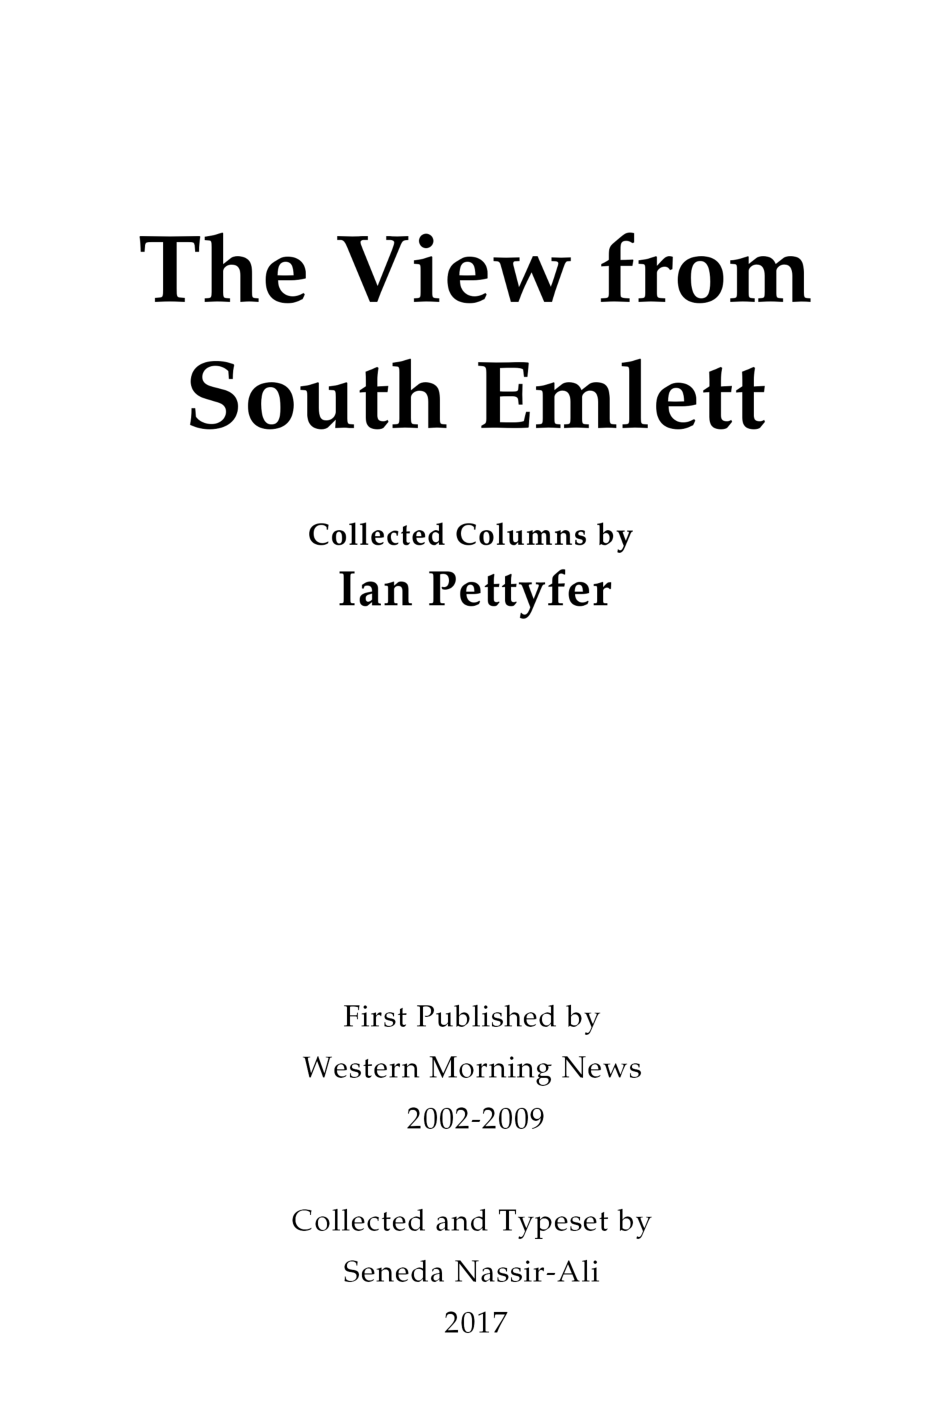
\includepdf{titlepage}
\mbox{}
\thispagestyle{empty}
\newpage
\pagenumbering{roman}
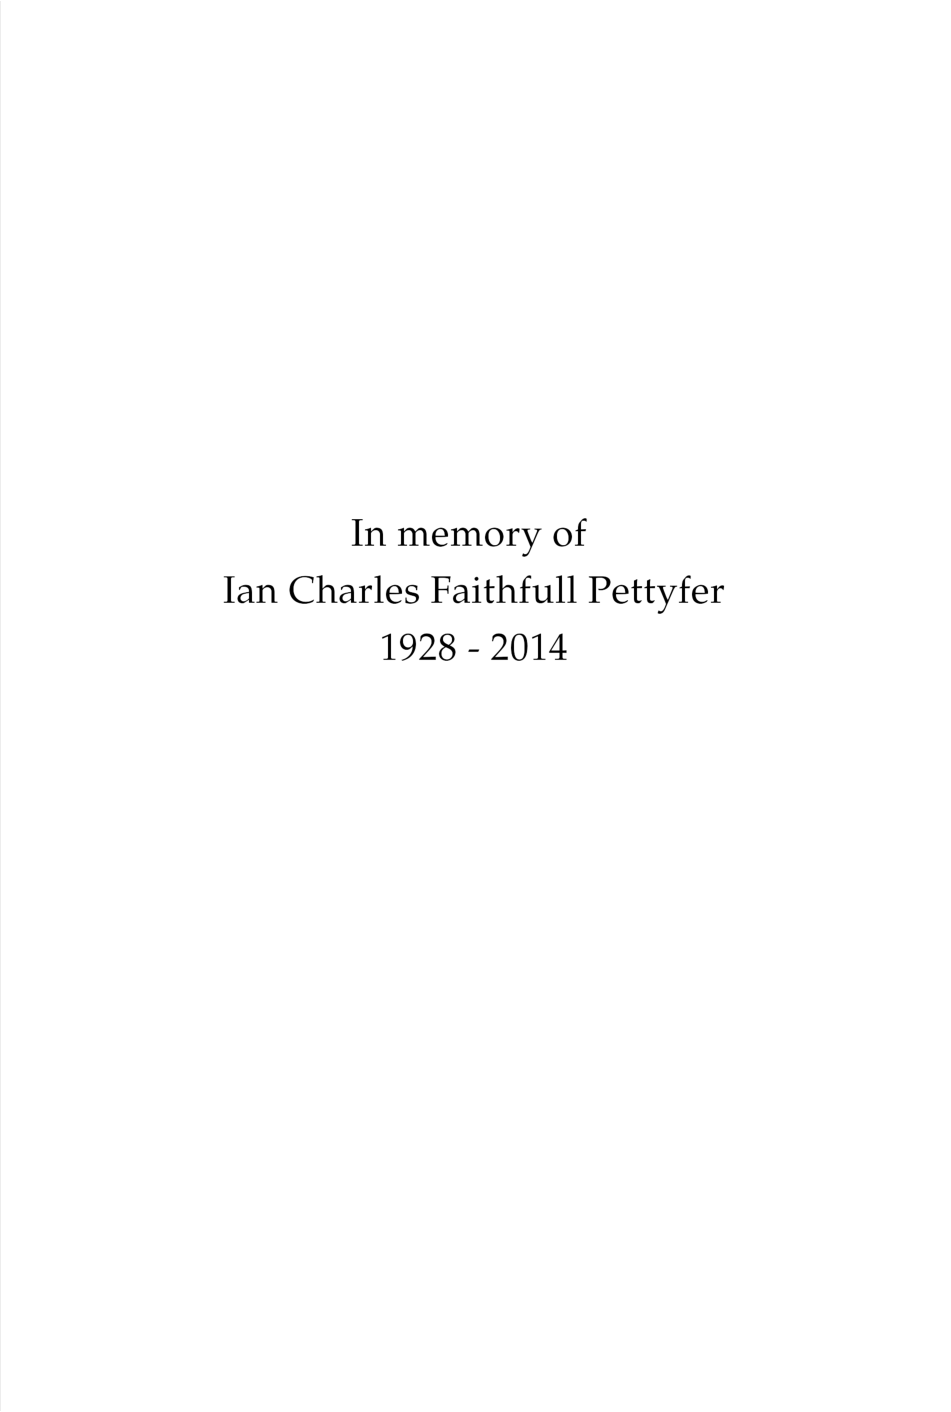
\includepdf{dedicationpage}
\mbox{}
\thispagestyle{empty}
\newpage
\tableofcontents*
\mbox{}
\thispagestyle{empty}
\newpage
\mbox{}
\thispagestyle{empty}
\newpage
\mbox{}
\thispagestyle{empty}
\newpage
\chapter*[2002]{2002}
\addcontentsline{toc}{chapter}{2002}
\pagenumbering{arabic}
\setcounter{page}{1}
\monthsec{July}
\Needspace{10\baselineskip}
\column{July 24th}{Jul 24th}{Just Another Layer of Complicated Subsidies}{24th}
I am a very lucky man. I live where I want to live in the middle of what I think is the most beautiful county in England. This is an opinion that is shared by many farmers in all parts of the country. We value the landscape that surrounds us, the fields, the woods, the hedges and trees, a patchwork view that has evolved over many centuries. It is not a contrived landscape like a garden or park, nor is its beauty due to any foresight on our part. It is the result of trying to farm profitably, to make the best use of every acre. And for me the pleasure in that landscape does depend to a great extent on how well the land is farmed. I see nothing very beautiful in a neglected farm, better if it were not farmed at all, but allowed to revert to nature.

    Now suddenly, something that has had an inherent value for all of us, town and country folk alike, has got to have an actual value placed on it. I refer to the `broad and shallow' stewardship scheme as envisaged by the Curry Report. By modulating (`Ministry speak' for reducing) our subsidy cheques, money will be available to pay us for cherishing (my word, the Ministry don't know that one) the environment. We will be able to claim for the work that keeps the countryside looking as beautiful as it has always done, or better still, as it used to do, and maintains or increases the wonderful variety of plant and wildlife associated with it. Of course it is not as simple as that. It would need a Solomon to even contemplate such a scheme. How do you reward farmers fairly in counties as varied as Norfolk and Northumberland? If we are all to be modulated we should all be able to access any scheme equally. A suckler cow gets the same payment in Devon as in Essex. And who will decide what a landscape should look like? Or whether one barn owl is better than ten yellow hammers? No doubt something will be thrashed out behind committee room doors and we'll start calculating how we can work the resulting scheme to our best individual advantage.

    And so it goes on, another layer of complicated subsidies. The ink is scarcely dry on Curry than our old friend Fischler, in the dying moments of his farm commission days, comes up with the idea of a single payment based on the past subsidies of each farm. God help us! What about the future and the young farmers coming in? Will they have to look for a farm with a good subsidy record? Perhaps it is not the young farmers that Fischler is concerned with, but the new entrants to the European Community, with no subsidy record at all.
    If you are not a farmer reading this, I have probably lost you already. I am pretty good at making simple things seem complicated; it takes years of practice filling in Ministry forms.

    What we do not need are any more fancy schemes. We already have `Sites of Special Scientific Interest', `Environmentally Sensitive Areas' and a `Stewardship Scheme' that between them are quite capable of delivering the varied countryside that the public want. Put more money into them, pay for the access, the footpaths and the wildlife habitats that farming provides. And pay a decent amount so that those of us who look after these aspects can make a proper living. If agriculture needs support, let's make it simple so that everyone can understand it. Why not an annual payment for every acre farmed, one rate for enclosed land and another for open land? We already have quite enough constraints on how we farm. If we want to modulate against the larger farms, and I would be in favour of doing so, use the number of people involved and employed as the yardstick for adjustment. The economists will say that is penalising efficiency, but so what? It is people we are talking about supporting and we need more people working in the rural areas, not just living there.

    And finally, if I may use as a metaphor the biblical story of Joseph and the fat and thin cows, let us hope that the politicians don't spend too much time tinkering with the Technicolour dream coat, but concentrate a little more on the message it contained. Years of plenty can easily be followed by years of shortage. With global warming and nuclear terrorism, who knows what the future holds.
\Needspace{10\baselineskip}
\column{July 31st}{Jul 31st}{Enough Basic Food Must Be Available for Poorest}{31st}
I watched the opening of the Commonwealth Games on television last week. The children of Manchester danced in the arena, David Beckham helped a little six-year-old girl, with a terminal heart condition and attached permanently to an oxygen cylinder, hand the Jubilee Baton to the Queen. A million pound fireworks display lit up the night sky. The late news followed. The first item showed pictures of the latest drought disaster to hit southern Africa, fourteen million people facing starvation, half of them children. Pictures of  little six-year-olds with swollen stomachs and skeletal frames who will certainly die before help can come.  Shots of empty grain stores following three years of no rain. I know the two sets of images cannot be taken together to put things right, life is not that simple. There are many other factors involved, HIV Aids, war and political instability. But as June Whitfield, one of the celebrities launching the appeal for emergency aid the next morning, is reported to have said `it is quite incredible that the public should be asked again to help'. And she is quite right.  This is not an unexpected disaster like an earthquake, forest fire or tidal wave. This is Africa where droughts happen all the time.

    As a farmer, I can clearly recall the '76 drought in the South West, with the grass fields turning to coconut matting, and yields of three hundredweight per acre and virtually no straw  from spring barley. That was after one dry summer, with little rain for six months. I try to imagine a situation here with no rain for three years. And I have to ask why those grain stores in Africa were allowed to become empty? Why is the Disasters Emergency Committee appealing for help now so late? There is no shortage of grain in the world. Our own national harvest just starting looks to be a bumper one and yet we are concerned for the grain market by the overhang of surpluses from the US and the Black Sea countries.

     And then the next evening I find myself pushing a trolley round our local Supermarket. The shelves are stacked with food from every part of the world. There is no space empty, nothing is out of stock. And pictures of those African children inevitably come into my mind. What happens to the food that is not sold, that goes past it's `sell by' or `display until' date? Do the staff buy it cheap, as I know they used to. Pig swill is now outlawed thanks to a Northumbrian farmer, who should never have been keeping pigs, but can farmers still buy the unsold vegetables for stock feed? I look for the manager and get the answer I am expecting. Company policy, everything past its date goes into the skip. Fresh today, land-fill tomorrow. As the song says, `what a difference a day makes'.  And again I know that this is not the answer to feeding the millions who would be appalled to see such waste. But surely we can do better, there must be ways of using this food here. Or is it the recently appointed Food Standards Agency that is enforcing rigid rules?

     Earlier last week it was reported that Lord Haskins, chairman of Northern Foods  and advisor to Tony Blair, has urged farmers to concentrate on markets that are large and real. I take that to mean we must produce food at world prices, never mind the constraints of farming to our standards of animal and environmental welfare. He tells us to be part of the global market, produce food cheaply. I suppose that might ease his conscience about chucking the surplus in a tip. Well, can I urge the Lord Haskins' of this world to concentrate on their responsibilities? If  the multinational bosses and  international money men want the freedom to operate world wide, if they claim globalization is a way of bringing prosperity to everyone, then they must take care to see that there is enough basic food and medicine available for the poorest  among us. They must not rely on last minute appeals to public charity when tragedy strikes. Otherwise their motives may be seen as self-seeking and hypocritical.
\monthsec{August}
\Needspace{10\baselineskip}
\column{August 7th}{Aug 7th}{A Case for Conventional Farming}{7th}
When news that the Government was going to invest millions in the future of organic farming hit the headlines last week, my first reaction was `good for them'. However, as I read on, I began to be alarmed by some of the extraordinary statements appearing in the press about what I would call `conventional farming'. And not only the national press, who love a good story if they can hype it up. Our regional press, including I am sorry to say, the Western Morning News, were making the most outrageous slurs about modern farming. Our editorial that first morning said that organic farming was a reversion to `good husbandry after years of exploitative pillaging of land and abuse of livestock which led to mass-poisoning of the land and the populace'. And the paper's main article the following morning by food correspondent, Mark Daniel, used phrases such as `the pursuit of cheapness at any cost has cost the health of billions and the lives of millions' and `local, fresh, organically produced food and drink taste 100 times better than the muck which is produced regardless of provenance and good practice'.

Now, come on. I, and a great many farmers like me, are not about to have the way we farm rubbished like this. Perhaps Mark Daniel might excuse himself by suggesting he was merely indulging in hyperbole. But this goes way beyond exaggeration. This is a load of twaddle.  We have doubled food production in the last 50 years to feed the nation, at, I thought, the nation's request. Where are the billions ill and millions dead that Mark Daniel talks about? Where is the evidence of mass-poisoning of land and people? It only takes three years to convert non-organically farmed land to organic status. A remarkably quick recovery for poisoned land.

And the lives of millions - what millions? If this a reference to BSE, TB or Foot and Mouth, organically farmed animals are no more immune to these diseases than any other animals. Any damage we might have done to people's health is more likely by producing food so cheaply that we have encouraged obesity. The vast majority of us farm under an assurance scheme of one sort or another, organic status is just such another. As we all know, the essential difference is the prohibition of synthetic pesticides and soluble fertilisers. The remaining rules are just standards of good husbandry which all of us aspire to. Some of us are better at it than others.  We have some bad apples and some shining examples of good practice among non-organic farmers. Farming is not black and white, as has been implied, but like everything in life, it is all shades of grey.

I am not opposed to organic farming. I started my career with three years studying the science and theory of agriculture under some very eminent professors, leaving with letters after my name in the hope of getting a well paid job. Why I ended up as a farmer is another story. But nothing led me to believe that the correct use of  fertilisers and pesticides was inherently harmful. Used in excess, yes, but most things used in excess are harmful. An excess of `organic' farming may harm our ability to feed ourselves.

We have friends and neighbours who farm organically. I respect their views and have always been open to conversion. In the early 60's we had an interesting family buy the small farm adjoining us, farming organically and producing the most outstanding tasting vegetables. Not a 100 times better, but certainly the best I have ever tasted. They were committed vegans, which made going to supper quite an event. It also made asking them back even more of an event. Geoff, who took me to Soil Association meetings and introduced me to some of the leading lights at that time of the `organic' movement, reckoned that the taste of his vegetables was due to the extensive use he made of seaweed fertiliser. I believe that is now banned under organic rules. The family left after a few years and emigrated to Australia. We were sorry to see them go although there were some compensations. The farm was bought by an airline pilot, who converted half the land into an airstrip and, in exchange for a regular supply of milk, gave me free flying lessons and the family free flights. We were also able to buy the other half of the farm, which he didn't need, at a ridiculously low price. We put all the land into permanent pasture, but I was very surprised at the serious infestation of docks and ragwort that it produced in the first few years. The docks we put up with, but the ragwort got on top of us and eventually we sprayed it with a weed killer. It is the only time I have used a herbicide on grass land in 50 years of farming. I didn't blame organic farming for the problem; I think the fault lay in the excessive use Geoff made of a rotovator as a cultivating tool, instead of ploughing. A pity he didn't uses horses - but then he was a vegan.

We buy our vegetables now from a well known local organic farm. The real difference to supermarket veg is the freshness. I might be quite pleased if Phil and Helen decided not to work so hard, deserted their principles and used a little fertiliser and spray occasionally. After all, if they are growing varieties that are resistant to pests and diseases, what are we eating. To be resistant involves plants producing chemicals that are poisonous to the insects or disease they are being challenged by.

I feel as strongly about organic versus conventional farming when it comes to the environment, but that will have to wait for another time.
\Needspace{10\baselineskip}
\column{August 14th}{Aug 14th}{Harvesting Was Much More Fun 200 Years Ago}{14th}
We are half way through our harvest; 16 acres of barley done  with 14 acres of oats to come. As I write, the rain is gently falling and I should be doing our Suckler Cow Premium application for this year. The harvest is nothing like the worry it used to be when we started farming. Then the corn was cut with a binder and left in stooks for two or three weeks. It needed another spell of dry weather to get it into a stack and was still a long way from being thrashed. Now the contractor rolls in with the combine, which seems to get bigger every year, and four hours later 16 acres of barley is in the corn bin. We used to make sure the gateways were wide enough but now the concern is whether the field is wide enough. We still have some two or three acre fields, but I doubt they will ever grow corn again. 

The other day, I was reading an account of harvesting 200 years ago. It was in `General view of the Agriculture of the County of Devon', written by Charles Vancouver in 1806. To paraphrase, it seems that when 10 to 20 acres of corn was ripe, notice was given in the neighbourhood that a reaping was to be performed on a particular day. A gang of an indefinite number of men and women assembled and, after a breakfast lasting till 9 o'clock, work started. By 11 or 12 o'clock, the cider had so warmed their spirits that the resulting revelry helped to attract more hands.

At one o'clock, dinner consisting of the best meat and vegetables, was carried into the field and distributed with copious draughts of ale and cider. Work went on from two till five  `without other interruption than the squabbles of the party', when `drinkings' were taken with buns, cakes and `all such articles as the confectionery skill of the farmer's wife could produce'. After `drinkings' (reminds me of a cricket match), the field was finished amid considerable noise and tumult, when the company retired to the farmhouse to `sup, carouse and vociferate until one or two in the morning'. The whole thing was repeated the next day at the next farm and so  on  through harvest time.

Not surprisingly, no wages were paid, but the workers were invited to a `harvest frolic', and at Christmas there was open house, which seldom continued less than four days and nights when the behaviour of the guests could be likened to the antics of a bear-garden. This must have been a considerable expense to the farmer and the authorities were not happy at the disorderly nature of the proceedings, but I suppose wheat was making a good price. It was around the time of the Battle of Trafalgar and we were having a little local difficulty with the French. Nothing changes!

Back to the Suckler Cow form. This is not a job I have been looking forward to as the penalties for mistakes get heavier every year, but is something beef farmers can not ignore. The premium is a very large part of our annual income. We used to have a young Ministry official (generally female) walk round the farm with a pair of binoculars to check the eartags of the animals we had applied for. I was quite happy to accompany them. Foot and Mouth put an end to that. Last year, unbeknownst to us, applications had to match exactly the records held on the passport office computer in Cumbria. Or you were in trouble.

We were informed in February that a mistake had been found on our application.  I phoned  Cumbria and was told that one of the heifers on our claim was, according to their computer, a cow. There was a two-year old calf somewhere in the country which claimed our heifer as it's dam. I pointed out that our heifer would have been one month old when it's calf was born; this was not merely miraculous, it was impossible. Not to worry, I was told, all would be corrected in due course. Doubtless when I put the phone down, the computer their end got a good thumping for allowing itself to be wrongly programmed. It did not even matter if the animal was a cow or a heifer, the premium claimed was exactly the same.

Come the end of May, I rang DEFRA to see if all was in order - the Suckler Premium was already overdue. We needed the money. Nothing doing. At the end of June, with July 1st the Commission deadline for payments to be paid, I wrote to Whitehall and was promised a reply from the Rural Payments Agency. Four weeks later, no reply. I wrote again, this time to the top civil servant at DEFRA. He is on holiday but I will definitely get a reply by August 9th. Oh yes? Nothing yet and I still don't know if the mistake, DEFRA's mistake, has been corrected. 

It is a desperate situation. Three quarters of the farmers in the South West who are owed Suckler Premiums for last year are unpaid. I understand that staff at the RPA in Exeter are working their socks off to get things sorted. Meanwhile DEFRA is accumulating fines of millions of pounds of taxpayers money for missing the deadline.

And our debts are building up as the months go by. We will get the bill for the combining soon. Perhaps we should offer our contractor an invite for four days open house at Christmas.

To help me do this year's  Suckler Claim, I have just received a print out from Cumbria of our animals currently listed on their computer. The only thing is, it doesn't show whether they are cows or heifers. Here we go again.
\Needspace{10\baselineskip}
\column{August 21st}{Aug 21st}{Vaccinate Our Badgers Now}{21st}
Over the years I have followed with interest, and sometimes with exasperation, the correspondence in these pages on badgers and TB. I have never, until now, felt inclined or perhaps dared is a better word, to join in. Are badgers to blame for the regular recurrence of TB in cattle in the south west, or do cattle occasionally infect the odd badger? The arguments from both sides have become more and more extreme, and I have been reluctant to get caught in the middle. But last week, a letter from one of the most frequent writers, Martin Hancox of Stroud, has stung me into the debate. He states that `no one has shown how badgers can give cows a respiratory lung infection in the field'. Well, I reckon I can and quite easily.

If I had any doubts, one incident which happened about three years ago convinced me. Badgers are a very common sight in our grass fields in the late evening, rooting for worms in the spots where old cowpats have decomposed. The field I was walking through had three badgers busy feeding and, as I had a camera with me, I thought I would try and get a picture. I got to within about a yard of one without disturbing it and bent down to get a close up, but the badger still seemed unaware of me. In order to get it to look up, I nudged it with my foot. The effect was immediate. The badger started back with its hackles up and gave a sort of coughing bark straight at my face. I was close enough to get spittle on my face. The badger ran off three or four yards before returning to attack my wellington boot. We then both retired in disorder and I never got my photograph. I have seen a badger do exactly the same when approached by a dog. Cows grazing in a field with feeding badgers certainly get the same treatment and their faces are nearer the badger than mine was. If that badger had been a TB carrier, then I must have been at risk. I know of no other British mammal that behaves in this way. 

However, I don't think this is the commonest route of infection from badger to cow. As I am sure Mr Hancox knows, infected sputum from a badger's lungs can be swallowed and the bacillus pass  intact through the gut, to be deposited in the badger latrines that we find close to the hedgerows of many of our fields. The bacillus will survive in the droppings far longer than it would as an aerosol. And, as every farmer will agree, the first thing a bunch of calves or newly purchased cattle will do on turnout is inspect the boundaries of the field, including sniffing along these badger toilets. 
Of even more concern is the evidence, which I have on very good authority, that older badgers have been shown to excrete TB in the last two or three years of their life, having been infected as young animals and recovered. I understand this happens in other species including man. The problem for cattle is that these old badgers, generally boars, get turned out of the colony by the dominant sow. They become wanderers, moving through other colonies, looking for food where they can against younger opposition, and ending up in cattle yards and feed passages with disastrous consequences. 

Twenty years ago, we had an explosion in badger numbers, which I attributed on this farm to the growing of maize as a forage crop. We now have over 15 badger sets within a mile of where I am writing; fifty years ago we had four which were never all occupied at the same time. We have given up growing maize and the badger population is noticeably declining. Much as we all enjoy seeing them, their numbers were becoming ridiculous. They were having a serious effect on other wild life and, I suspect, each other. If we are unfortunate enough to find TB in our cattle, and I am tempting fate as we have never yet had a reactor, killing badgers would for me be the very last resort. Nor do I agree with the argument often put by farmers that we are doing badgers a favour by killing off the diseased ones. Badgers are extremely tough animals and, if not stressed, can take TB in their stride.

What we urgently need are vaccines for both cattle and badgers, especially badgers, to begin to eliminate the carriers. I understand Ireland is already well down this route - why don't we co-operate? Meanwhile the Krebs trial is a total waste of time. It will result in huge expense, countless badgers killed to prove something we already know, and TB out of control while we wait. If society wants to consider badgers as sacrosanct, payment for consequential loss will have to be made.
\Needspace{10\baselineskip}
\column{August 28th}{Aug 28th}{All is Safely Gathered in}{28th}
Last week saw our harvest completed, with the straw, which we value nearly as much as the corn, safely baled and in the barn, and all before a bright harvest moon reached full. We have had a good year so far. The summer has suited us, with rain at regular intervals to keep our steeper pastures from burning and not too much to interfere with silage and hay making. We have enough of everything to face whatever the winter might throw at us, or am I tempting fate? What a difference this is compared with last year, when we had too many animals stuck on the farm, thanks to `foot and mouth'. We went into last winter with about half our fodder requirements and ended up buying silage and straw in the spring. I wonder how many people outside farming realise how long it takes to get back to where we were 18 months ago, when the F\&M horror all started. And beef and sheep farming wasn't going a bundle then.
         Meanwhile, the outside world is worrying about global warming, a vast cloud of brown smog is hanging over south east Asia poisoning millions,  and the `great and good' have gathered in Johannesburg  at the Earth Summit to talk about it all. Will it result in just more hot air?

         It reminds me of a hot air balloon ride I was lucky enough to win in a raffle several years ago. There were seven of us, including my daughter Cath and her partner David. Our pilot introduced himself as Arthur Street and I said I believed him. It seemed a very good name to give to an irate geriatric farmer like me, when making a landing in a bunch of stampeding cows. He assured me he was actually the nephew of the late great A.G.Street, farmer and author.
         We took off from `George's Field' in the middle of Exeter. It was a fine, hazy late summer's afternoon with little or no wind. We were hoping to fly in the general direction of home, about seventeen miles north west, and view the familiar country side from above. I always think how boring England looks from an aeroplane. I suppose there is nowhere high enough to give any perspective but perhaps floating along a few hundred feet above ground in a basket might be better.
         We went up smoothly to a thousand feet but remained directly above Exeter. Arthur said  there should be a southerly wind if we tried going higher. The ground slowly receded into the haze and at two thousand feet we suddenly emerged into a clear blue sky with no sign of Exeter at all. Instead we were sitting on a platform of pavement coloured smog which looked solid enough to walk on. Apparently this is quite normal in still weather over any city and is the height at which the particulates of exhaust fumes settle out of the atmosphere. Maybe I haven't explained that strictly accurately, but the sheer volume of filth we must be breathing every day in town can never be better visualised.

         Needless to say, we never did find any wind, and landed four miles away in Upton Pyne. And not in the middle of a herd of cattle, but on the edge of a cornfield. We came down so gently that the men in the party were able to get out holding onto the basket and walk the balloon into a quiet country lane, where we folded up the canopy and stole away with nothing to show that we had ever been there.
         I was going on to write `how nice it is to breathe clean country air', but Jim, my son, has just come back from Eaglescott airfield in North Devon, to say his flight in a microlite, a present from my daughter-in-law, has been cancelled due to poor visibility in haze. It looks a fine August evening from the ground. So even out here we can't escape the pollution.

         Are we as farmers contributing to the problem? Do our tractors throw out more exhaust fumes than they used to? The answer has to be that they don't. Our tractors today are certainly bigger and more powerful than there were in the past, but engine efficiency has improved enormously. With the larger implements they handle, the time it takes to get through the various tilling and harvesting operations has reduced out of all proportion. I only have to stand on our hill and listen. I used to hear tractors droning on from every direction on almost every day in the summer. Now silence is the norm with bursts of activity from time to time. Most of the noise comes from those fuel guzzling monsters in the sky.
\monthsec{September}
\Needspace{10\baselineskip}
\column{September 4th}{Sep 4th}{When It Comes to Politics Take a French Lesson}{4th}
Last week saw our rams in with the ewe flock. This is very late for us; we have for many years put the rams in soon after shearing with a view to catching the early suck-lamb trade in late February or March. We are able to keep our small flock of ewes and lambs outdoors through the winter on mowing grass, without supplementary feeding unless it snows. This has given us the best lamb price, does our light land good and takes the pressure off our silage and hay acres in late spring early summer. However two things have persuaded my daughter-in-law, who manages the sheep, to change the system. Firstly we are still recovering from the mismanagement of the flock last year when we were forced to keep our lambs on the ewes until May or June. And more importantly, the very good trade we used to get at Easter seems to have slipped in recent years. The price we received for the last few lambs we sold in late May this year was considerably better than the price we got in March. What caused this I don't know. Did the export trade to France restart at that time perhaps? 

         I am sometimes asked by non-farming friends why farmers export live lambs for slaughter to France, instead of as carcasses. I tell them that we ourselves never sell fat sheep, or cattle for that matter, other than direct to an abattoir, the nearer the abattoir the better. That is because I have always preferred deadweight marketing through a farmer co-operative. However, before I give my friends an impression of being `holier than thou', I do go on to make it clear that our prices depend on the liveweight market price of the day. And the French, who are our best customers, prefer to eat lamb that is slaughtered close to home, their home. If the French are to be denied the right to buy lamb through an agent at a British livestock market, the regulations on the transport of live animals would need to be tightened up even more than they already are.

          I also point out to my non-farming friends that all the farmers I know would be delighted if animals destined for slaughter could go direct to the nearest slaughter house, so long as we were guaranteed a fair price for what we produced. Unfortunately we do not live in a perfect world, yet.
         However I have to admit to having a sneaking admiration for the French farming community. They certainly know how to make their Farm Ministers toe the line. And it is not just the fact that French people as a whole are more rural minded, this is becoming less and less relevant. When we have travelled in France by car on the rare holidays we have managed in the past, we have made a point of staying at farm `bed and breakfast's. It has been amusing to see the reaction of the rather grumpy, and often smelly, farmer to the news from his appeasing wife that the guests on this occasion are also farmers. Out comes the Calvados and the dictionary and we are discussing how to solve our respective problems until after midnight. The only snag has been the inevitable tour of the farm the following morning, before we can continue on our way. 

         And it is clear that they have as many ridiculous rules and regulations imposed on them as we have. Our problem is that we do not seem able to get our politicians, whether Labour or Conservative, to understand how to work the system in Brussels. I have to take my hat off to them for keeping our beef out of France for so long, never mind a fine they will never pay, and nearly managing to keep our lamb out as well, (that would have sorted out live exports for the animal rights lobby).

         I wonder how French farmers are viewing the proposed  `Liberty and Livelihood' March on Sun, Sept 22. If you must have a march, why on a Sunday and not on a Monday, I would expect them to ask. Tell Londoners to take an extra Bank Holiday, while you exercise your right to roam. That might give politicians something to ponder on. And I would agree with them. Rotten eggs left in the House of Commons car park as a reminder of the visit, would also be on their agenda. We may well be glad of the French before much longer, if the hints coming out of the Johannesburg Conference are correct. I believe Margaret Beckett has suggested a rapid reduction in CAP spending to allow Third World Countries to sell Europe cheap food. Who is that going to help? Third world farmers as well as first world farmers need to sell food at a proper price. If anyone is going to block that stupid idea, it will be the French.
\Needspace{10\baselineskip}
\column{September 11th}{Sep 11th}{Ministers Have Proved to Be a Big Failure in Recent Years}{11th}
"If farmers do not receive extra cash for their milk, supplies will run down, forcing up the retail price". Words from Ben Gill, NFU President, or the Chairman of one of the larger farmer Dairy Co-operatives? No, a quote from Lord Whitty, Food and Farming Minister, in a cutting from last week's Times newspaper, which was given me by an outraged neighbour. The short piece said that Ministers fear that milk prices could rise this winter as poor rates for dairy farmers trigger an exodus from the industry. So Lord Whittey has unwittingly, if you will pardon the pun, come clean on Government policy. Do nothing for agriculture unless it affects the price of food. If we peasants can carry on producing milk for peanuts, that's OK. So long as supplies are sufficient, he can fold his arms and flannel his way out of awkward questions when accosted by desperate farmers.

           However, what interests me more about Lord Whitty's wording, if that is what he actually said, is the inference that the farm price for milk could go up without an increase in the retail price. Where would any extra cash come from? The milk processors? They are already being squeezed by the supermarkets, and I doubt the supermarkets are going to suddenly become generous out of the goodness of their hearts. Oh yes, they have got hearts, but theirs are of the accountancy kind; share holders and senior management first, staff and shoppers second and suppliers last. So what on earth does Lord Whitty mean?
           What he will find out, if he does not accept that retail prices must be encouraged upwards with all the weight Government can muster, is that he may be held responsible for a massive increase in milk prices when a shortage eventually occurs. Perhaps is he assuming we can import sufficient fresh milk from the Continent at current UK prices or even persuade people to switch to European style UHT milk. Doesn't he realise that as Food Minister, he is responsible to the nation to see that a milk shortage does not occur.

          Sometimes I really do despair at the Farm Ministers we have suffered from in recent years. The last one did seem to listen with some sympathy, and even appeared to understand at times, but melted away like summer snow in the heat of the Foot and Mouth crisis, when it really mattered. His predecessor came storming in with New Labour, refused to meet anyone at grass roots level and made decisions that were grossly unfair to some of us, without first checking the facts. I remember being asked with other farming representatives to meet his most junior Minister for breakfast in a swank hotel in Plymouth.We were each allowed to bring up one subject of concern while he progressed through his bacon and eggs without comment. When we had all finished talking and he eating, he informed us that his secretary, who had been taking notes,would be in touch with us. He then spent some minutes lecturing us on our folly in not ensuring that this posh establishment sold  local beer. We took great pleasure in pointing out that like most farmers, we couldn't afford to find out what sort of beer a place like that served.

           I am not being party political in making these criticisms. In my opinion, the worst Minister of the lot recently was the last Conservative holder of that office. The sight of him on television, dressed like some Australian bush wacker, trailing round the capitals of Europe behind our then prime Minister trying to get our beef back on track after BSE, must have made us the laughing stock of every farmer in the EU. Our industry has been through a very rough ten years but fate might have allowed us at least one good Minister in that time. Oh for a Tom Williams, a Lord Amory or a Jim Prior.

         We also had the Prime Minister's farming guru, Lord Haskin, pontificating on the milk situation last week. For once I agree with him when he suggests that we need just two or three large farmer milk co-operatives instead of the plethora of groups we seem to be getting, following the assasination of Milk Marque by Stephen Byers. I thought Lord Haskin had a hand in that; what a pity he didn't speak up then. Milk Marque was only about 50\% of the supply.

           Eventually I am sure we will achieve some kind of market stability for milk. The Milk Marketing Board was born out of severe hardship for smaller producers, and what a rock that proved to be for the whole livestock industry. We can't go back to that, but time is running out for many of us.
\Needspace{10\baselineskip}
\column{September 18th}{Sep 18th}{No Shortage of Wildlife}{18th}
The other day I dug a grave for my wife. Well, actually, my wife asked me to dig a grave for her old sheepdog, Sammy, who had come to the end of a long and I hope, happy life. Of all the pets we humans keep, many have a rotten existence, but working sheepdogs seem to have the best of it. They do what comes naturally, appear to thoroughly enjoy their work and are remarkably faithful to one owner. We have always had sheepdogs through the years we have been farming, but I expect Sammy will be the last. Jenny handed over the management of the flock a few years ago to our daughter-in-law, so any successor will have to belong to her. It used to amuse me sometimes to find that a geriatric Sammy had staggered down to the farm late in the evening and was standing looking at the sheep in the lambing shed, when he should have been taking a quick turn round the house before bed. What was he thinking about or was he thinking at all? I assume they were happy memories.

         As usual on these occasions, I dug the grave for Sammy at a spot where we wanted to plant a tree at some time in the future. That was two reasons for making a good deep job of it, even though the ground was very dry and hard. I was surprised, therefore, and not a little annoyed to find three days later that badgers had excavated poor old Sammy. I reburied him even more thoroughly but to no avail. I have always understood that badgers will avoid a very potent human smell, particularly hair or urine, so following this second reburial, I myself took a turn round the house before bed for three or four nights and this seemed to do the trick. Not a very dignified way to treat Sammy's grave, but when the devil drives. Unfortunately the badgers eventually came back and I had to pile large stones over the spot to finally defeat them. Planting that tree will in the end be a bigger job than I had anticipated. I shall certainly remember Sammy!

           Am I sure it was badgers? Yes, there is no question of that. We have plenty of badgers at present. They wander round at night, knocking over buckets, looking for kitchen waste and seeing what they can find in the cattle barns. Recently I found signs that one had got into the roller-mill shed where I hadn't bothered to block the entrance. I went down after dark the following night with a torch, intending to give it a good fright if it was there again. I surprised it all right; four large badgers thundered out  nearly knocking me off my feet. A fifth went twice round the grain silo before reluctantly ambling off into the night.

           Environmental critics of modern farming would be surprised if they were to look round our farm for evidence of loss of wildlife over the last fifty years. It is true we are less intensive than we used to be since switching from milking to suckler cows, but we use some inorganic fertilisers and cereal-weed sprays, and the usual medicines for the stock as we always have done. We have pushed out hedges when paid to by Government and reclaimed bracken and gorse infested ground like all our neighbours. But the numbers of wildlife species has remained remarkably constant. 

         We currently have 56 species of birds nesting on or near the farm, we recorded 25 species of butterfly last year, and 22 species of mammals. These are not my figures, but were compiled by a long time friend and naturalist, Ken Tyson. Ken worked for the Institute of Grassland and Environmental Research (IGER) at North Wyke, so he understood the pressures that modern farming puts on the environment. He was a prominent member of the Devon Wildlife Trust, a keen ornithologist, and played an important part in the Devon Branch of Butterfly Conservation. Sadly, he died very suddenly in June at the early age of 66; we shall miss him greatly and not just as a friend, but for the wealth of information he gave us about what was going on around us naturally, which we were generally too busy to notice. He would comment on the way we could make small adjustments which might benefit certain species.

         What is apparent over recent years is the loss of some ground nesting birds, such as the wood lark, partridge and wild pheasant. We still have some skylarks and yellow hammers nesting, but they are not as plentiful as they used to be. We have also lost our hedgehogs and we rarely see a hare now. I have no doubt the cause for this decline is linked to the growing of maize. We started planting maize in the early seventies, initially for strip grazing as there were no contractors equipped to handle it for silage round here. It was very obvious straight away that badgers thought Christmas had started arriving early. We were not too bothered as, although we had four badger setts on the farm, we were not aware of them as a nuisance and rarely saw them unless we went badger watching when the young came out in early summer.

         However, within a very few years we realised that something a bit dramatic was happening in our badger population. New sets were appearing all over the farm, badgers could be found feeding in the middle of the day in midsummer, often in very poor condition, and at night almost every field would have a few badgers in evidence. At its peak, we had about fifteen setts in use, and once counted eighteen badgers feeding in a nine acre field.
         The pressure for any creature breeding on the ground must have been intolerable. We stopped growing maize about ten years ago and the badger population is now declining. I suspect that not only were many more young badgers getting through their first winter by fattening up on maize cobs, but that sow badgers were breeding younger as their condition encouraged the late implantation of the ovum. The net result was too many badgers with too small a food supply through the remainder of the year.

         There are other examples of changes in wildlife populations having a marked effect on certain species. I am sure that grey squirrels and magpies, either non existent or heavily controlled years ago, are responsible for the decline of some of our more popular songbirds. And I have recently discovered that the increase in numbers of roe deer, grazing brambles in our woodland, are the probable cause of the loss of our white admiral butterflies.
          We need young Ken Tysons or David Attenboroughs to regularly visit all our farms and discuss with us what they find. That would do more for the future of the nation's wildlife than all the Stewardship Schemes put together. It might also stop some of the rubbish theories put about by self styled experts.
         In any event, we are not short of wildlife here. Our resident hornets have nested this year under the eaves outside our bedroom window. When you find hornets in bed with you, as we have, who needs Viagra?
\Needspace{10\baselineskip}
\column{September 25th}{Sep 25th}{DEFRA's 30-page Booklets}{25th}
Recently we received a thick envelope containing a 30-page booklet about the welfare of laying hens. It came from DEFRA HQ in London, so I resisted the temptation to throw it away unread. The accompanying letter explained that all stockmen are required by law `to be familiar with, and have access to, appropriate welfare codes'. How did the powers that be know that we keep half a dozen hens, which look after themselves around the farm buildings laying their eggs in the most inaccessible places? The letter says they used information collected as part of the agricultural census, but we haven't done one for years.

         At a quick glance, I could see nothing that had any relevance to our system, except that we obviously were well up on the `Five Freedoms'. What a total waste of paper. And something similar is coming through the post on a weekly basis. At the height of the Foot and Mouth crisis, anything from DEFRA would have been welcome, if only to prove they were there.

         However, a more sinister package arrived a few days later. I expect every farmer has had one of these. It was entitled on the outside `Nitrate Vulnerable Zones: Important information enclosed', and my heart sank. Yes, it contained the usual 30-page booklet. Have you noticed that these ministry booklets always have about 30 pages? Is it assumed that less than that and we will not take them seriously, but anything larger will exceed our attention span? This one was glossier than usual and was accompanied by a detailed map of our area of North Devon.

         For once it was our lucky day. The map showed that our land is almost exactly bounded by the edge of the designated zone. One field further and we would have been in it, in both senses of the well known agricultural expression. We farm near a watershed. On one side of our approach road, water initially flows south but, strangely enough, reaches the sea at Barnstaple. On the other side, our side, water flows north but ends  up at Exmouth. Why our side is cleaner than the other, I have no idea; I would have expected the Taw catchment area to be less intensively farmed than the Creedy. I must remember in future which side of the road I am on, if I get taken short on the way home late from the Pub. I wouldn't want to make any extra difficulties for my neighbours.

         However, for farmers caught up in these regulations, this is no joking matter. I read through the guidelines and I have to wonder whether this will not be the final straw for some. At one point, it states that ``You are required by law to meet the obligations in bold text". The booklet has chunks of bold text on nearly every page. One of the more simple examples reads ``Do not apply nitrogen fertiliser to steeply sloping fields". It goes on to say, but not in bold text, to assess the risk before spreading nitrogen fertiliser. Some eastern counties farmers I know consider that nearly all our land is steeply sloping. The booklet wriggles out of this problem by stating that no specific angle of slope is given in the legislation, but steeply sloping fields are unlikely to be cultivated. Our steepest field grew wheat in 1890. We gave up making silage in it some years back because the neighbours complained that we interfered with their work. They felt they had to watch as they could see whoever was tractor driving through the roof of the safety cab.

         Perhaps I am making too much of all this, but I wonder if people outside farming really understand what we have to put up with, when they hear us complaining about the red tape that is throttling us. I know it happens to all sections of society, but when I started farming, one of the attractions for a newcomer was the absence of form filling. Having finished school, college, exams, what a relief to join a profession that didn't need to do any paper work; even income tax was levied without doing accounts, `Schedule D' I think it was called.

        To think I would end my career like this. There is one consolation. Like most farmers, who farm as if they'll live for ever, one hopes that the next generation will carry on. If I didn't wade through the worst of the stuff that comes through the post, I think my son would have packed it in long ago. He is beginning to believe that it's a plot to get rid of all of us.
\monthsec{October}
\Needspace{10\baselineskip}
\column{October 2nd}{Oct 2nd}{Give GM Crops a Chance}{2nd}
If I was a young man again, would I go farming now? Without hesitation the answer would be ``Yes". Am I mad? My wife says ``Undoubtedly, but then you always did like a challenge." And the way things are, a challenge it certainly would be.  Being a farmer has always seemed to be the most enduring occupation one could choose. The air we breathe is all around us, although it can be pretty horrible in some places. Water basically falls out of the sky, but the third essential for life, food, has to be produced on a day-to-day basis unceasingly. You would expect agriculture, therefore, with an expanding world population, to be the safest profession to join. It may not feel like that in Britain at the moment, but I have absolutely no doubt that circumstances will change. 

 There is one aspect of society's view of food production at the present time, however, that really does worry me. Groups of well-meaning people seem to spring up every time there is any radical advance in technology, and trumpet the alarm in the most strident tones. I expect it has been happening since we learnt how to make fire without waiting for a lightening strike. No doubt, in those days, the more anxious members of the tribe got together and stamped it out before it set the world alight. But there was space then to go away quietly and try it out with nobody looking. Now, anything new is world news within hours. Of course you have gathered that I am referring to genetically-modified organisms. 

 I can well remember a similar situation arising when artificial insemination was developed in the late 1940s. One of my professors at university at that time, Dr John Hammond, was a very well-known geneticist. He lectured on animal reproduction and was, unlike some of the professors, a most amusing and accomplished speaker; his lectures were packed to the gunnels. He was one of the foremost scientists at the time involved with the separation and storage of semen, to allow the development of vast numbers of offspring being sired by one superior animal. I think I am right in saying that the Milk Marketing Board was financing some of the research. The days when a runner, generally me, was sent to the owner of the local village bull, informing him that we had a cow bulling and could he come immediately, with bull, have long gone. And what a staggering difference to livestock farming that has made. 

 One of the asides that Dr Hammond used to include in his lectures, was an update on the abusive letters he had received from members of the public on the subject of AI. Apart from the personal attacks on his moral and religious beliefs, there was real and, no doubt, very proper concern about the effect the use of such techniques would have on human reproduction. Babies without known fathers, accidental inbreeding, loss of natural human diversity, development of a master race, and so on. And all perfectly possible. The feelings expressed were almost the same as we are getting about GMOs today. Should we have stopped then and should we stop now?  I am one of those who think that it is impossible to put the genie back in the bottle. We have to go on, but make sure we know what we are doing and control properly those who are doing it. The idea that we should try to make Britain a GMO-free country is about as daft as stamping out that prehistoric fire.  

Imagining myself as a young farmer starting tomorrow, I would want the chance to develop and use the enormous potential that these new techniques could bring. In fact if we were to go down the road of a blanket ban in this country, I would emigrate immediately. No one disputes that there is a lot wrong with the way the technology is being developed at present. There cannot be any sense in allowing the patenting of life forms which gives some multinational companies a licence to print money. But the possibilities to improve life on this planet, in its present predicament, are mind-blowing. Genetic engineering within species could produce food plants that are naturally resistant to pests and diseases, fix their own nitrogen requirements, become perennial instead of annual, are salt tolerant and produce increased yields, in a timescale that could make all the difference to the future.  So my message, as a young farmer, would be don't ban it, but make absolutely sure it's done right.
\Needspace{10\baselineskip}
\column{October 16th}{Oct 16th}{Stepping Stones Through the States}{16th}
Jenny and I landed in Boston on our way to see my brother in British Columbia. Watching our approach from the plane window in the hope of getting an aerial view of the city, there was a moment when I thought we were going to splash down in the Atlantic. The runway seemed to emerge from the waves as the wheels touched and the Captain apologized for having to brake so sharply due to a shortened runway. I suspect he meant that we were landing at high tide. If sea levels rise at all, with global warming, Boston won't have an airport. Faced with similar problems on that scale, one wonders why the U.S. government doesn't accept the Kyoto agreement. In fact, the many Americans we talked to on our long sight-seeing train journey across the States seemed just as concerned as we are in the U.K. with their government's reluctance to join the rest of the world on this issue.

When we last visited my brother, who has lived and worked on Vancouver Island for the past 30 years, we came home by train across Canada, stopping on route wherever we felt like it, and taking a fortnight to see as many places and talk to as many ordinary Canadians as we could, before flying back from Toronto. We so enjoyed the experience that this time, 15 years later, we thought we would attempt to repeat the journey in the opposite direction in the States, which we had never visited. The idea was to travel by train from east to west, and then stay with my brother for a couple of weeks before flying home. Amtrak, the company that operates the passenger rail service in the US, offers a thirty-day pass costing 250 pounds for rail travel anywhere in America. Boston, from where Britain started its journey home over 200 years before, seemed the right place to start.

Getting through immigration proved easy enough, although with a passport photo having some slight resemblance to Bin Laden's father and a place of birth listed in Pakistan, I did expect some reaction. The immigration form we filled out on the plane included the question, and I kid you not, `do you anticipate being involved in any terrorist activity during your stay?'. However our answer to the question about being on a farm in the last ten days did get us out of the queue pretty quickly. Seeing the notices plastered all over the airport about keeping Foot and Mouth out of the country, we were expecting a little local difficulty, but the soles of our shoes were all they inspected. I have to say I was disappointed at losing the chance to report back on the stringent disinfecting procedures we were forced to undergo. I even volunteered the information that our farm had been within two miles of an outbreak, but to no avail and we were sent on our way with the usual American blessing of `have a good day'.

Boston proved to be a good choice of city from which to start, on what was to be a zigzag tour of the northern half of the U.S., dictated mainly by the Amtrak timetable. We had decided to give each of the cities we visited one whole day only, using them like stepping-stones across the continent, with a `day' or `day and night's travel between each, and planning ahead only one step at a time. Boston we gave two days to buy our rail pass and find our feet.
  
The city is smaller than I had expected. In fact all the American cities were smaller than one visualizes. But Boston, of all the cities, seems most conscious of its place in history. The feeling that it was here that America first discovered its identity is everywhere apparent. A little boat, looking no bigger than a Brixham trawler, a replica of the one from which the 60 tons of tea was thrown overboard, in protest at British taxes, is moored in a harbour so small it is no wonder that the resulting mountain of tea, which rose well above water level, caused more problems for the British Governor in loss of navigation than loss of revenue. What a pity the Welsh didn't throw more beef burgers into Holyhead dock. The name of the midnight rider, Paul Revere appears on every landmark; the monument on Bunkers Hill to the first independent battle, which was fought on the wrong battlefield and lost, and `Old Ironsides', America's most famous battleship, is awash with tourists. But, as we were to find everywhere we traveled, the people were extraordinarily friendly, the good food was expensive, the fast food was diabolical, the weather was a heat wave, the air-conditioning was freezing, the toilets were called rest rooms. And we were enjoying our holiday. We moved on to our first view of the American countryside and New York.
\Needspace{10\baselineskip}
\column{October 23rd}{Oct 23rd}{Hurricane Adds Miles to American Saga}{23rd}
Leaving Boston on the first leg of our sightseeing journey to Seattle, we boarded the train for New York with some little apprehension. This first and shortest step would determine whether we would survive the next 5000 miles. Jenny is a great train enthusiast. She enjoys the freedom of movement and seems able to sleep on a reclining seat while I tend to fidget around trying to get comfortable. Happily the first impressions were favourable. Passengers are shepherded on board from a station waiting room and found a seat by a train attendant, as if joining a plane. The coaches are roomy and the seats comfortable, the dining car and buffet food sufficient, if uninspiring, and the toilets (the only place in the States they are not called rest rooms) clean, at least at the start of each day, and spacious for the `Ladies'. Our 250 pound travel pass only allowed us `coach class', so we would have to survive the nights on the longer stretches; upgrading to first class for a sleeping berth for just one of the nights would cost us more than the whole trip put together. Looking out at our first view of the American countryside, which was monotonous enough to allow us to get out the Amtrak timetables and route maps, we decided we could make it.

I will try not to bore you with too many details of our wandering. Writing this from the comfort of my brother and sister-in-law's house on Vancouver Island in British Columbia overlooking the sea, with the salmon jumping while they wait to go inland to spawn, I feel I could write a book. Next year I will probably find it difficult to fill a postcard. Suffice to say, we traveled down the east coast, stopping first at New York and Washington. We gave each a full day for sightseeing, New York by bus and river tours and Washington on foot. New York is unexpectedly the most welcoming city I have ever visited, building upwards the most natural form of expansion on a small island, and the pavements permanently crowded with friendly people. Strangely, for a country bumpkin like me, it was the only city anywhere in the world I would wish to live. 

What we saw of Washington is not really a city at all, just a loose collection of Government buildings, splendid in themselves, and monuments and museums. We did find ourselves outside the Department of Agriculture, but it had wisely closed its visitor centre ten minutes before we arrived. The White House I found to be surprisingly small and even more surprisingly accessible. It was almost within sight of our hotel, which itself proved interesting. On arrival we had had difficulty in finding a moderate hotel with a room available. We ended up in one with scantily clad statues outside, startling red decor and wall-sized mirrors in the bedroom. Its proximity to the embassies had us wondering as to the exact status of the place! After this we generally booked a day ahead if possible.

After Washington, we journeyed south through Virginia, staying at Williamsburg and Charlottesville, and on through the Blue Ridge Mountains, where the endless conifers really do appear blue as they reach the horizon. We had now been travelling for a week but further progress south was blocked by hurricane Isadora coming ashore from the Gulf of Mexico at New Orleans and disrupting the rail system; we therefore turned north to Chicago. The heat wave, which had been with us since Boston, came too! So far we had seen very little evidence of serious farming; a few small fields with a couple of black cows here and there, but everywhere, shielding our view, nondescript trees with the odd scattering of clapboard houses. People we talked to seemed very conscious of the prolonged dry weather and the effect it was having on farming. Having a catfish sandwich in a cafe in Charlottesville, which was under severe water restrictions, we were even charged 25 cents for a glass of tap water. (We soon learnt that a sandwich meant a full sized meal - enough for two.)

However for all the talk of drought, we were coming into the basin of the great American rivers, with first the Ohio, which flowed past us as we rattled through the night to the `windy city' of Chicago. From there we headed southwest to St Lois and crossed the mighty Mississippi to follow the Missouri for 100 miles to Kansas City. This was a most memorable part of the trip, viewing a river that had been over a mile wide while still 1000 miles from the sea until, according to our train attendant, the early settlers arrived to enclose it with embankments and make it navigable. We were also at last coming into farming country, field after field of corn (grain-maize) and soya, some harvested but much not yet ripe. The fields gradually increased in size, and although continuous, were never larger than about 100 acres, with hedge type boundaries of straggly trees or uncultivated strips.

We were lucky on our way north from Kansas City to find ourselves in the viewing lounge seated next to a retired Ohio farmer and his wife, who were returning home from a visit to an ailing brother in Arizona. He was over 80, but still helped his stepson at harvest time. He had started life as a produce farmer, as he called it, on 400 acres. He had depended on immigrant labour, but increasing regulations had forced him to switch to maize and soya. He explained the simple rotation, that we could see from the train, of disking and fertilizing after harvest to encourage any weed growth, which was then spray killed and disked again in spring before sowing with added nitrogen. (We never saw a plough or ploughed ground in all our travels.) He was pleased his own son had a good job outside farming, and his stepson had an eight-hour a day job besides farming the 400 acres. He felt the future for farms his size had gone. You either farmed as a manager for big business or rented the land to larger units. He wryly commented that he could earn more than the going rent by putting land into environmental schemes! Where have I heard that before?  The couple had never travelled before by train, usually they flew to wherever or went by car, but age had persuaded them to take the slow option. We found this repeated time and again; over half the Americans, young or old, who we met on Amtrak were new to rail travel. It is no wonder that Amtrak is having serious financial problems with its long distance passenger routes.

We left our farming friends and changed trains at the small country town of Galesburg and headed west for the mile high city of Denver.
\Needspace{10\baselineskip}
\column{October 30th}{Oct 30th}{Nothing Great About Steaks}{30th}
At Galesburg, Jenny and I boarded the California Zephyr to San Francisco. This was one of Amtrak's superliners or double-decker transcontinental trains, with passengers on the upper deck and services and baggage on the lower. Galesburg, where we had to wait 6 hours to make our connection, was a pleasant country town, about the size of our home town of Crediton, with a wide main street that needed little imagination to take one back to the 19th century. There were no tourists and it actually rained! 

The countryside from Galesburg continued very much as it had from Kansas City, field after field of soya and maize, some harvested, some hardly ripe. The crops looked very average at best and in places distinctly poor. The dry summer had certainly made an impact and I saw nowhere I would wish to farm. The field size did get larger as we travelled west, but it might do some of the politicians, who preach farming at world prices, no harm to see the desolate landscape this produces.
  
We had decided to break this 2000 mile stage of our trip at Denver, partly to avoid spending two consecutive nights on a train, but also to see if we could get a decent steak at a reasonable price. After all, Denver boasted to be the cattle centre of the world and to have the finest steaks in the world. Rolling into Denver the following morning, we could see the  extensive cattle pens beside the railway sidings - what about the steaks? The countryside had changed overnight to more open plain with scattered cattle here and there, and a few small feed lots, but we saw no great numbers of animals. We were now one mile high and the air as we left the train felt delightful, after the heat of the previous two weeks. Denver's economy now relies on tourism and high-tech industries, which did not bode too well for that cheap steak. And so it proved. 

The restaurants in the splendid new pedestrian shopping mall, where we ended up after finding a hotel and having a brief look at the sights, were distinctly expensive and very fancy in their menus. There were steaks, but always on some sort of bread with sauces and cheese on top. After trying half a dozen places, I finally blew my top in one and asked where we could get a straight steak flat on the plate with some chips and mustard. That brought out the cook, who said he would oblige if we liked to come back later. I wondered how much extra that would cost, but fortunately Jenny saved the day and found a small bar away from city centre that was happy to oblige. One 14 oz well matured Angus rib steak char grilled with fries \textsterling6 - not bad. But I doubt if it was pure Angus and I've certainly had better steaks at home. So much for Denver.

The next day, we got back on the train and up and over the Rockies. And what a fabulous day's journey that was. We climbed swiftly to 9000 feet; at one point, to gain height, doing a `figure of ten' according to the viewing car commentary, (`two over the eight' perhaps?). The first snow of the autumn had fallen the night before, and the fir trees had a light covering. The train goes through the 6 mile Moffat tunnel, the longest in the world when first built, but the early settlers with their covered wagons had to go on up another two or three thousand feet to cross the passes. Looking at the terrain, it is difficult to imagine how they ever made it, but it was explained that they went very slowly, only a mile or two a day at the worst places, and that they took up to three years to reach California.

The scenery from here on was spectacular - through Boulder Canyon, following the Colorado River, past ski resorts, to more open cattle country between the mountains. The cattle we saw were generally black, but I would hesitate to claim them if I was an Angus breeder. We went through Salt Lake City, which I would like to at least have seen from the train, unfortunately at night and reached Reno the following morning.  Here there was a 20 minute stop to stretch our legs while the train crew changed over for the final day's run, and then on again through more great scenery in the Sierra Nevada, over the Donner Pass and down to the flat and fertile land of California.

As you would expect, this was by far the best farmland we had seen. There were great tracts of arable land, many cattle, cows with calves, sheep, fruit trees, vines, affluent looking farmsteads, an air of prosperity, but I still wouldn't want to farm there. There was a sameness about the countryside, mile after mile, with little real variation. Until you see the alternative, you don't realise how lucky you are, and the British public certainly don't realise how lucky they are to have us farming the way we do. Let us hope they realise before it's too late.

San Francisco proved to be a slight disappointment after all we had heard about it. The hotel room was the worst so far, the heat wave had caught up with us again, the trolley ride over the famous undulating hills was packed with tourists, and there was a huge rally in the park against `War with Iraq' (we found no American throughout our trip who was for Bush, we were constantly asked why Blair was backing him). Worst of all, my digital camera vanished on a crowded trolley-bus on the way to catch a ferry across the bay. I only realised it as I went to take a picture of Alcatraz - was that a chuckle from a long-dead inmate, or was it the slap of  a wave against the bow? The camera was insured, but oh for those 100 pictures from Denver onwards. And the Golden Gate Bridge is nothing to the Clifton Suspension. We did however find the best ever Farmers Market right in the middle of the city. I know now that `dry farmed' tomatoes are those grown without irrigation - a better selling label there than organic.

On we went once more on our final leg, a night and day ride to Seattle.
\monthsec{November}
\Needspace{10\baselineskip}
\column{November 6th}{Nov 6th}{Final Leg of the US Saga}{6th}
We are home again at last. Five weeks is the longest holiday we have ever managed in 50 years of farming. The winter corn is tilled and up, the cattle and sheep are all looking well, and the bookwork is up to date. That is one good thing about growing old -  you can take a long holiday without being missed! There is only one cloud on the horizon - the Visa bill from America, which is due any day.

The final 24 hours of our American train journey, taking us  from San Francisco to Seattle, started in the evening, which meant that we missed seeing 400 miles of  some of the best Californian farmland along the Sacremento River. As daylight came, we were into Oregon and the Cascade Mountains. We stopped to change crews at the small town of Kalmath Falls, which is over 4000 ft high and lucky enough to have an unlimited supply of  water from hot wells, with a temperature of  95°C at a depth of 60ft.  This is used to heat the entire town  through the winter and even the roads are kept free of snow with hot-water pipes beneath the tarmac.

Another 50 miles and we were passing through Crater Lake National Park. This must be a bird-watchers paradise, with 250 species of bird recorded here and 50 pairs of bald-eagles regularly nesting. Dropping down into more open country, with vast areas of plains grass interspersed with Ponderosa woodland, we were told to watch out for a large herd of buffalo, which had been introduced into the area in recent years. No luck unfortunately, plenty of cattle but with 30 miles to the horizon to hide in, the buffalo kept out of sight.

We now came to our last piece of spectular scenery, and for me, possibly the best. The train joins the Columbia River Gorge at a great height above the river and slowly descends over the next 40 miles to river level. The autumn leaf colours of the aspen and maple were  at their best. A young lad of about eight sitting next to me said he intended to be a farmer when he grew up. He was returning with his family to a small holding near Kelso, where the Columbia River runs out to an area of farmland very reminiscent of England. I confess I gave him every encouragement to pursue his chosen career. It cheered me up to listen to such enthusiasm from a youngster and at least he has ten years to think better of it.

We arrived in Seattle at 10.30pm, two hours late, but fortunately with an hotel-room booked  in advance. The city gives the feeling of being at the hub of an area of the fastest economic growth in the US. The computer giant, Microsoft, is located in one of the suburbs, and Bill Gates, its founder and the world's richest man, has his home there.

We were advised at our breakfast cafe (it is very rare to get breakfast in an hotel in America) to see the Pike Street Farmers market before catching our bus on to Canada, and it certainly proved a worthy final attraction. `Farmers' is perhaps an incorrect title, since it is open daily on three floors of a large building on the waterfront and sells virtually everything from innumerable stalls. The main event, which is apparently famous nation-wide, is a fresh fish stall, which features the three stall holders hurling a ten pound salmon to each other through the crowded bystanders. This can be very disconcerting if you find yourself in the line of fire. I didn't see them sell much fish, but a British Lions rugby union scrum-half might learn a thing or two.

We travelled on that afternoon to be met by my brother in Vancouver, to enjoy a fortnight's holiday at his home on Vancouver Island. Jenny reckons she could have gone on for another week on a train, but I was thankful to at last get two consecutive nights in a bed. I shall spare you any further details of our trip, although we did have one interesting visit to a Charolais herd near Courtenay, which opened our eyes to the absence of red tape in Canada. More on that, perhaps, and my overall impressions of the US, another time.

We had an uneventful overnight flight back from Seattle, packed in like sardines in a can.  Just as we were boarding, the security officers decided to pull a few of us out of the queue and give us a very thorough going over. Shoes off, trouser belts undone, pockets emptied, hand luggage spread out over a table and sifted through, and a body search (or feel, rather). I found humour proved the best defence, and even got my scissors passed as being my shaving tackle, but some of the other victims looked distinctly starchy. 

At Heathrow we saw no officials of any description, no mention of illegal meat imports or `Foot and Mouth', and just a rainy windy English morning to greet us.And, in spite of being dog tired in a crowded bus running late on a crowded motorway, it was impossible not to appreciate the beauty of  our own English countryside, getting ever better as we came west to Devon.
\Needspace{10\baselineskip}
\column{November 13th}{Nov 13th}{Time to Get Together}{13th}
It seems that nothing has changed on the farming political front during our five weeks absence from the UK. I suppose I shouldn't be surprised, although I did expect that echoes from the Countryside March might still just be audible. We knew it took place; we saw a brief picture on an American TV news of the crowds in London, with the caption ``Toffs march in defence of their sport". Was Government moved at all by the show of feeling which the number of people taking part was supposed to generate? Without access to back numbers of the newspapers, I shall never really know. Certainly, statements from Ministers or Government spokesmen seem as negative as ever about the future of farming. 

Margaret Beckett, at long last pinned down by the Western Morning News, says she does care about the farming industry, but I see nothing in her interview with Jason Groves to suggest that we are expected to produce the bulk of the nations food. In fact, the news on Friday of the British Government-backed ``arms for agriculture" deal with Thailand implies the exact reverse, if it is true that Britain has agreed to negotiate a reduction in European hygiene standards to help Thailand export more food. 

And that other `bete noire' of British agriculture, Lord Haskins, is still predicting that thousands of small farmers will be driven out of business over the next few years. Note that word `driven'; I presume he means that economic circumstances will persuade them to leave farming for another profession, but it does sound a bit like some sort of  Government `pogrom'. No mention of retirement schemes or help to make the transition to larger farm businesses.

However, for me, the most depressing news to come back to is the emergence of yet another farming political pressure group - ``Farm". I won't go over  ground well covered by Anthony Gibson in these pages last week, but I do feel that a lot of the blame for the emergence in recent years of so many different voices speaking on our behalf, and, as a result, very often muddling the real message, does lie with the NFU. Anthony may or may not agree with me, but his position as NFU Regional Director does preclude him from giving his own opinion on this.

I have been a member of the NFU for over fifty years. I have done my stint as a branch office holder and, more recently and surprisingly, three years as a county office holder. I think, therefore, that I am fully entitled to criticise the only organisation that has any real hope of  getting through to the politicians and the people of this country before it is too late.

To do that, we have got to get all these disparate groups together to speak with one voice. And to do that, in my humble opinion, Ben Gill, the leader of the largest, oldest and best financed farming organisation, needs to be big enough to admit that the NFU has failed in the past to fully represent all our members by ensuring there was a proper balance of interests on NFU's governing Council. He could then embrace, if that is the right word, all the Farmers for Action, Family Farmers, Small Farmers, and other farming associations on an equal basis and get a proper dialogue going. 

In so doing, he might well lose his position as President at the NFU AGM in February, but he will have done more for all of us than anything he might achieve with two more years in office. Perhaps he is already down this road; I am no longer party to the inner workings of the NFU, if I ever was. I do know that I am probably making myself unpopular with many friends in the NFU by suggesting that we should admit to any past failures. There is no denying, however, that it has been virtually impossible in the past for a family farmer, with no employee or adult children to help, to become an NFU Council member. Considering the proportion of farmers that could be categorised in this way, it is a disgrace that the constitution of the NFU was not changed years ago to correct this imbalance. Had it been, I can think of many areas where decisions on policy might well have been very different.

In the last three years, I am glad to say, the rules governing the election of Council members have been altered. All members now have a postal vote, and there is no requirement for would be candidates to work their way up through the various regional committees to be selected as a suitable representative to go to London. The question of proper payment for the time involved needs to be addressed, but at least the Michael Harts and David Handleys of our industry can now take a full part in the NFU at the highest level, before feeling the need to set up small focused groups as a criticism of the one organisation which should speak for all of us.
\Needspace{10\baselineskip}
\column{November 20th}{Nov 20th}{Restaurant Waste Raises One Weighty Discussion}{20th}
I was asked  the other day in our village shop - yes, we still have one, thank goodness - by a friend who had read about our recent rail journey across the States, whether I hadn't found America `vast'. I said this was not a description that immediately sprang to mind. We only really travelled through the northern half of  the country, and did not see the ranch lands of Texas or the deserts of the south west states. 

The Great Plains, which we crossed in about ten hours, is only 700 miles from east to west, and although it is almost continuous flat arable farm land, it is broken up into distinct fields, with nowhere a single crop stretching to the horizon. The only place I have been which I would describe as vast is the prairie land of Alberta in Canada. Crossing that by train, some years ago, we could look out of the window as it got dark, at a combine harvester in an endless crop of wheat and, the next morning, wonder for a minute whether the train had stopped over night, and we were looking at the same combine in the same stretch of wheat. 

There was, however, one aspect of the States where the description `vast' might be accurate. I must be careful here in my choice of words. I wouldn't want to offend the extremely friendly people we met everywhere we went; we have the other half of their country yet to see, preferably after winning the lottery! I am referring to the physical appearance of  too many young Americans, most noticeably in the eastern cities we visited. To say they were overweight would be an understatement. They looked reasonably fit, attractive and well dressed, although their choice of clothes sometimes left little to the imagination. But some parts of their anatomy could only be described as gigantic, which is as polite as I can put it.

I know we have a problem here with obesity in young people, and health authorities in all the rich nations are voicing concern on the long term effects on human health, but this was something else again. I don't think the fast food  industry is the only culprit, although I am pleased to see that `McDonalds' is changing its ways somewhat by going over to waitress service and extended menus. 

In America, everywhere we went we were given very large portions and, judging by the other diners, expected to leave what we couldn't eat to be thrown in the trash bin. In fact we hardly ever saw anyone clean up their plate, it appeared to imply to the restaurant that their portions were meagre. I have always felt that leaving food indicated that one didn't like it - a throw back to war time rationing perhaps - but we found that, by explaining that we were on a budget, we could easily get a single portion split onto two plates without even a raised eyebrow. 

One interesting Chinese `breakfast and lunch' restaurant we found in Washington sold meals by weight - so many dollars a lb. The food was excellent, the coffee was free, and having loaded your tray from a huge range of choices, you placed it on a scales and paid accordingly. That was one place no food went into the bin. It was crowded and the owner, who was happy to explain his philosophy said he saved a great deal of time since nothing needed individual pricing. It was also pretty simple at the check out. I hope the idea catches on, I don't like the attitude that food is so cheap it can be thrown away.

Obviously it isn't only the quantity of food that is to blame for obesity, poor quality must play a big part in turning people off  healthier eating. It was very encouraging to see how well patronised the weekly city food markets were, in both the US and Canada. They were manned by farmers rather than semi-professional stallholders as is often the case here, and the produce was first class. I was a little puzzled, however, at the rather vague way the term `organic' was used to describe most of the produce on offer. The farmers implied, when asked,  that they farmed organically, but it seemed to be their own interpretation of that system of farming, rather than any set of rules that they were following. They would be breaking the law in the UK.

While we were there, it was announced that the US Department of Agriculture was setting new standards for what qualifies for an `organic' label, so no doubt this anomaly will be put right. More interestingly, because of the increased bacterial resistance to antibiotics in humans, Senator Edward Kennedy is sponsoring a bill to ban the use of all antibiotics in farming, except for the treatment of sick animals. It was estimated that the cost of producing meat without the use of antibiotics would average \$5 to \$10 a year to the consumer. Perhaps the use of hormones in beef production in the US will be banned next - wonders will never cease.
\Needspace{10\baselineskip}
\column{November 27th}{Nov 27th}{When Foot and Mouth Was Just a Fact of Life}{27th}
I can well remember, in the spring of 1951,  standing on the top of a hill about a mile from where I am now writing and being shown a large depression in the ground. I had just started farming and, having enjoyed a welcoming supper, was being given a stroll round his acres by my neighbour. What did I think that was? A bomb crater I guessed. No, that is where all the animals were buried after a `Foot and Mouth' outbreak on the farm in 1935. It had apparently made little long term impact on the farm or the neighbourhood; outbreaks occurred from time to time but the perceived wisdom then was that no farmer went bust after going down with the disease. The compensation allowed one to start again with improved  breeding stock; remember in those days there was no A.I. and quality in farm animals often left much to be desired.

My next experience of F\&M was 1967. The disease had broken out in Shropshire and was spreading south. This was, for those days, a very serious outbreak. It was decided by farmers that we should disinfect the wheels of all vehicles crossing the Devon border, in an attempt to keep the disease out of the south west peninsular. With the help of  local NFU branches, we were formed into teams of three or four people to operate four-hour shifts at check points on every road into the county.

So it was that I found myself, with two friends, on a dark night on the road between Taunton and Bampton doing the 2am to 6am watch. Very little happened until it started to get light. The odd passing car was quite amenable to being stopped. After driving slowly over a layer of disinfectant-soaked straw, its wheels were sloshed with disinfectant from a watering can. But the early morning lorries were generally not so helpful. The drivers were impatient to get on and told us we were wasting our time. Some charged straight through our signals, staring fixedly ahead or even giving us the V sign. We decided that long distance lorries were probably the most dangerous contacts and must be made to stop. Two of us, therefore, stood in the middle of the road with our backs to the oncoming traffic while the third stood by with the watering can. It worked - it takes a brave lorry driver to knock down two people with a witness watching. F\&M never reached the south west, but whether we made any difference we shall never know. We all got home safely - `road-rage' hadn't then been invented.

Will we, I wonder, talk so flippantly in the years to come about what farmers and the rural community have been through in the last 18 months? The '67 outbreak seemed just as dire at the time. There were horrendous pictures in the media of piles of burning carcasses; a slaughter policy was considered as efficient in dealing with the disease as continental vaccination methods, where the disease occurred more often.

There is one big difference this time that will leave an enduring bitterness. I am referring to the bungling inefficiency of our political masters with which the whole sorry saga was handled. What an irony that many of us, who had escaped the disease, began to wish we hadn't. 

Like many farmers, we were heavily overstocked as the summer wore on, with over-fat lambs and beef cattle grazing our silage and hay fields and no hope of making half enough fodder for the coming winter. After the worst appeared to be over, we were suddenly served with a `D' notice, effectively closing us down for three weeks. It could not have happened at a worse moment - we had fat cattle long over due for slaughter, which were licensed and booked to go.  Apparently there had been a case in sheep on a farm 25 miles from us, in a parish which already had an outbreak. A lorry had delivered feed to that farm the day after visiting us. The sheep were diagnosed one day after that. In vain I argued with the Ministry of the nonsense of attributing the infection back to us. With a minimum three day incubation period, and no sign of disease in our animals, how could we possibly be implicated. But no, the rules from London stated that any farm visited by a feed lorry up to 48 hours before an outbreak must be issued with a `D' notice. 

A month later, with our `D' notice cleared, the animals were licensed again and ready to go. This time, the license was revoked at two hours notice, because the status of the abattoir had been changed in London overnight. Yes, we could still send the animals to the same abattoir but we needed a different licence form. It would take two days to obtain. We lost our place in the queue of farms waiting to dispose of animals long past their prime. If you can believe it, three weeks later when we thought we had finally cracked it, the abattoir at Torrington burnt down. I suppose I should have expected it - our cattle were due there the next day. At least, that couldn't be laid at the door of the Ministry.

Although we had to buy tons of extra feed, we were one of luckier farms. Many suffered far far worse from the cock ups caused by officials in London making decisions, the implications of which they had not the faintest notion. Perhaps it was unfortunate that a General Election got mixed up in the plot. Or that the spectre of BSE still hung over us. Certainly the contraction of the State Veterinary Service by previous Conservative administrations had a considerable bearing on the way the outbreak was handled in the field. Whatever the reasons, the horrors of that summer will remain with us all for many years to come. I hope the F\&M report from the European Parliament is the final one. It is time to close the book. We must now ensure that the lessons really are learned this time.
\monthsec{December}
\Needspace{10\baselineskip}
\column{December 4th}{Dec 4th}{Farming is for the Birds}{4th}
This week we are starting to bring the cattle in for the winter. We normally keep them out as long as possible into December, which shortens the winter tedium of strawing out the covered yards and cleaning the feed passages. Our light land doesn't poach easily and the cattle are much healthier living outside, but my son, Jim, has decided that, with near record rainfall in November, enough is enough. Following the horrors of last year, we have reduced our suckler herd down to 55 cows and 90 followers, which, on 250 acres of pasture, would  be considered by most farmers as being very under stocked. The cattle also have access to about thirty acres of woodland at the edges of the pasture fields, where they can shelter in the worst weather. A few years ago we had 85 suckler cows plus followers, and even with that number we were farming very extensively. 

As all beef farmers will agree, every beef animal we sell at current prices is making a loss. It seems the only way to stay in business at present is to farm so as to obtain as much of the EU beef subsidy money as we are entitled to, while keeping the number of loss making cattle down to a minimum. This is a quite disgraceful state of affairs now, but if the politicians have their way and phase out production subsidies over time, pure beef production in this country will eventually disappear altogether. Unless, that is, alternative support systems are put in place which will allow us to go on producing what is best for this farm. If we are to farm here in the way that society sees as appropriate to the English countryside and, at the same time, produce food at world prices, then there has to be some system of support. 

With this in mind, Jim applied 18 months ago to join the `Stewardship Grant Scheme', which is all that is available at present as an environmental alternative. We have just completed our first year of a ten year plan. In our case, we are continuing to farm very much as we always have, but with the fencing and hedge laying being paid for, for a change. As our fields only average about eight or nine acres, we are probably earning as much from this as most, but this would nowhere near replace the direct subsidies we get for our beef production if these are to disappear. There are other aspects to the Scheme which pay us to stop applying any manure, organic or inorganic, to certain fields and to restrict grazing to specific times of the year to encourage wild flowers. We are even paid to fence off some areas altogether from cattle to encourage other forms of wildlife; that's OK by me if it is considered the correct way to spend money from the public purse, but it won't produce much beef. The Scheme, which on the whole seems to be working well, needs considerably beefing up, if I may put it like that, if it's going to do the job.     

I suppose that is the thinking behind one of the ideas that came out of the `Curry Report' on the future of farming. The new `Broad and Shallow' Stewardship scheme that will be available to all farmers in three years time and which is going on trial on 50 farms in the Tiverton area is the result. I understand that to qualify, farmers will merely have to demonstrate that their system of farming is benign to the environment in their locality. As we are already in another Scheme, it seems we are to be excluded from benefiting, no matter that we, ourselves, are currently paying for this new scheme through modulation. But I am not losing any sleep over it; it is going to be hardly worth bothering with, if the figures I have heard are correct. I suspect it will be a case of `Shallow' by name and shallow by nature. 

I would, however, like to know who is actually dreaming up the criteria for qualifying for this new scheme. The nine people who have been appointed to the Implementation Group of the Sustainable Farming and Food Strategy do not strike me as being experts on environmental matters, (with a title like that, who needs a committee). If I may pick out one instance that particularly gets up my nose, why do we just have a representative from the Royal Society for the Protection of Birds on this new Quango. I have nothing against the gentleman in question, he may be admirably suited to the job for all I know, but I thought the RSPB was a single issue charitable organisation. I see that his qualification on DEFRA's press release is put as simply that. I have every respect for the aims and achievements of the RSPB, but I see no reason why my profession should be saddled with their particular concerns. I suppose it accurately sums up this Government's view of the future of British agriculture - farming is for the birds.
\Needspace{10\baselineskip}
\column{December 11th}{Dec 11th}{Wrath of Bird Lovers}{11th}
Last Friday, I went as usual to collect our weekly box of organic veg from Phil and Helen at Linscombe Farm. If they are not too busy, I quite enjoy arguing the pros and cons of organic farming. I was, therefore, somewhat taken aback to be hailed by Phil, before I had hardly opened the car door, as the `man who hates the RSPB'. Apparently that was the impression I had left him with, after reading my comments last week on the Government's appointment of Graham Wynne, of the RSPB, to the new body overseeing the changes to the food and farming industries.

I was intending to write about something else this week, but if that's how it appeared, perhaps I had better put the record straight. I love birds, I wouldn't dare say otherwise. As Phil pointed out to me, birds are a good, though not the only, indicator of the health of the environment. I am not a member, but I am all in favour of the RSPB and the work they do in keeping birds at the forefront of our attention. I believe they have by far the largest membership of any society in the UK. (I guess if they were all to vote one way in a general election, they just might affect the colour of a new government - perhaps Tony Blair is conscious of that.)

Having said that, I have to confess to being irritated by the way any variation in bird numbers is generally portrayed as a decline due to modern farming. Without farming many of the common birds wouldn't be here at all. The skylark, that defining bird of good agricultural practice, which we have in small numbers at present on our farm, would certainly disappear very quickly under a tide of oak and ash forest.
 
What worries me far more than changes in the way we farm, is the effect modern life is having on birds in this crowded island. I don't really give a fig for the cirl bunting, which has been brought back from near extinction with great effort on farms in the Kingsbridge area. It is a  small uninteresting species, which I believe is common in Europe, a relative of the yellowhammer, a much prettier bird, that is itself in decline on farmland. A bird I really care about is the nightingale.

Jenny complained a while ago that she had never heard a nightingale and you can't go through life without hearing a nightingale at least once. I don't think there are any left in Devon. There used to be some nesting on the common at Chudleigh Knighton, but when we were there some ten years ago, we heard nothing but the traffic on the Exeter to Plymouth dual-carriage way.

So  a year ago last spring, we went to Walliswood, a small hamlet in Surrey between Horsham and Guildford, where I lived as a teenager. It was famous for the number of nightingales nesting there, so much so, that in early May it was almost difficult to get to sleep at night for the noise they made. It was where the BBC used to make recordings for background to nature programmes. I have to admit that we locals used to feel like throwing an old boot into the bushes sometimes to shut them up.

When we arrived, things looked hopeful. More people perhaps, but Surrey was always overcrowded. The farm land and woods looked comparatively unchanged. However, a chat with the daughter of the farmer I first worked for, did not auger too well. She had not heard a nightingale in years. Nor had anyone in the house where I used to live or in any of the pubs in the area. We listened well into the night at all the likely spots, before we realised that we were hearing airliners passing over head at regular intervals. We were on the flight path of Gatwick Airport, ten miles away.

We found our nightingales a few days later, about thirty miles away in west Sussex. We put our heads in at the door of a 16th century pub and asked if they knew of any thereabouts. Two pairs in the garden at the back and one in the front was the answer. There was a double room either side, with a bathroom in between - we could take our choice. An old boy drinking in the corner said his nightingales were louder than the pub's, and he could do us a room cheaper. The breakfast menu and the bath, a 7ft iron one the likes of which I last saw watering cattle, settled it - the back room in the pub. The nightingales sang all night. As someone once wrote `that marvellous crescendo on a single note which no other birds attempt'. At dawn a couple of blackbirds, those finest songbirds of all, joined in and, by the time we got up, a nearby rookery was providing the chorus.

So, if you have never heard a nightingale, I suggest you go there next spring. The pub is at Balls Cross, five miles north of Petworth. Who knows - they may already be planning a new airport or motorway in the area. A few more years and you could be too late.
\Needspace{10\baselineskip}
\column{December 18th}{Dec 18th}{Times That Seem a World Away}{18th}
Christmas shopping - not my favourite occupation. That sounds like Scrooge, but you know what I mean. It's not buying the presents; it's the full car parks, the shoulder to shoulder crowds and the check-out queues that get me down. But not this year. 
We went to Exeter to  combine our shopping trip with a visit to the Royal Albert Memorial Museum, where there is an exhibition on at present called `Love, labour and loss'. It shows 300 years of British Livestock Farming in Art, starting with paintings by the likes of Turner, Constable, Landseer (could he paint animals) and others, and goes on with a collection of the familiar paintings of  those monstrous farm animals like the `Durham Ox'. 
The exhibition takes up five galleries and brings one right up to the present with a photographic record of  the trauma of FMD on one west Devon farm. I could have done without Damien Hirst's `Dead calf in a tank of formalin'; it looks horribly prophetic but I doubt if any livestock farmer would regard it as `art'. That aside, it is a great collection, and the shopping seemed to go well afterwards.

For me, the exhibition inevitably brings back the memories of  a life's time farming  in Devon. What an extraordinary 50 years to have lived through, with, I think, greater changes in that time than all the previous years put together.
I remember my first Christmas here. I don't recall exactly the work on that particular day, but we must have done the morning milking as usual. We had eleven cows, ten Guernseys plus a Jersey belonging to Nancy, the wife of my partner, John. (In case you are wondering, Jenny was in the future - she was still at school.)

We milked by hand, the cows being tied up for the whole winter in a shippen, which was normal for those days. Thank God for Nancy, she could milk twice as fast as John or me, and just writing about it brings back the cramps in my hands.
After milking, the milk churns were tied to the luggage rack of the car and taken the two miles to the milk-stand at the end of our lane. It wasn't so much a case of hurrying to catch our `Channel Island' milk lorry, which went early, as making sure we beat Jasper Colton, our neighbour, whose lorry went later. If he got out into the lane first, you'd  had it. His horse never went faster than a walk and there was nowhere to overtake. He would look steadfastly ahead, sitting on his churns in the butt-cart, but I suspect he had a smile on his face. Occasionally the laugh was on him. The end of our lane slopes down into the main road, and on icy mornings, his horse had difficulty stopping. The sight of the horse sitting down  in the shafts of the two-wheel cart, with Jasper struggling to keep his churns upright was almost worth missing the lorry for.

The morning chores of cleaning out the shippen, bedding up and feeding the cows and young stock, the three saddleback sows, and the deep litter hens, didn't take very long. However that still left the job of cranking up our old spade-lug Standard Fordson tractor and driving out to the root field to cut enough `marrow stem' kale with a machete to cart back for the cattle. For Christmas, the hay would have been cut out and fetched the day before from which ever hay-rick was currently open. We made hay with a sweep and hay pole, which meant stacking out in the fields. 

With the evening milking finished, the essential day's work was done. That first year, John's Uncle Dick had come down to join us. He was a bachelor schoolmaster from Bolton and he had brought his housekeeper with him to cook our Christmas dinner. She was a German lady of fair size and middle years, which is the kindest way I can describe her. I think her name was Helga and I have no idea how she got from Germany to Bolton. Uncle Dick had also brought down a super petrol Tilley lamp to help with the farmhouse lighting. He didn't think much of ours, which were the normal paraffin models.

With no mains electricity, and a limited supply of water from a surface well, Helga was still sure she would give us a meal to remember. I have absolutely no recollection of  the main course, but instead of  Christmas pud, we were going to have apple strudel and doughnuts. To do that, Helga said she needed a very hot Aga, so the Aga draught control was put on full from early morning. By the time we got in after the evening milking, the kitchen was unbearably warm, the Aga was going like a blast furnace and Helga had used about a months ration of phurnacite nuts. And she was going to need about three weeks butter ration to make the doughnuts.

Its incredible now to remember that over five years after the end of the war, we were  still rationed for almost everything - meat, fats, sugar, petrol, coal, and, I think, clothes. Even cattle, pig and poultry feed required ration tokens. However, to hell with rationing, it was Christmas.

Uncle Dick seemed to have disappeared. ``He's in the cupboard under the stairs" said John. ``He's trying to light his Tilley lamp. He says this farmhouse is so draughty, he can't get the petrol to vaporise. He's brought aviation fuel specially, it gives an even brighter light." We had a thatched roof but at least we had the telephone connected - it was number 13, the last one left on the local exchange. Not that I think a fire engine would have got to us, lorries couldn't get down our lane in those days.
Happy days. That was Christmas that was, but I wouldn't go back.
\chapter*[2003]{2003}
\addcontentsline{toc}{chapter}{2003}
\monthsec{January}
\Needspace{10\baselineskip}
\column{January 1st}{Jan 1st}{A Future Full of Optimism}{1st}
Christmas is a time for nostalgia, but not all my memories are entirely happy ones. There have been years when, with the overdraft, unpaid bills, and ever-present cows to be milked, I have  regretted, on Christmas Day, not having chosen another profession. But New Year's Day always seems to give my spirits a lift; things are bound to get better, the days are starting to get longer or perhaps I am just an eternal optimist. And certainly if you are a farmer at the present time, an optimist you have got to be.
    
I was amused therefore, the other day, to read a  150 year old article from a reprint of the first edition of  `The Field'. It was dated 1st January and entitled `Agricultural Prospects for 1853'. It included the sentence `There is nothing to be done with a class which feels itself defeated and dispirited, for under feelings of disappointment and despair the most rational and practical plans of improvement are dismissed with disgust, almost without examination'.

What an uncanny echo from the past. The article begins  by saying that the prospects for 1853 were decidedly cheering. This was the opinion of farmers at the Smithfield Show of that year; that the worst was over, that any future legislative changes must be for the better, and that prices ``must continue steadily on the advance". I didn't go to Smithfield this year, so I don't know if there were any similar feelings in the show-going farmers of today. Certainly, if my memory of agricultural history is correct, those ancients were right to be optimistic, they were at the start of the 20 years that are now described as the `golden age' of British farming. Even in the depression that followed, due largely to increasing food imports, there seems to have been opportunities for enterprising farmers to get on in the world.

My father-in-law used to enjoy regaling me with tales of his family's move from a small farm in Cornwall when he was a lad of fifteen. Apparently there was the chance of a tenancy of a thousand acre farm in Hertfordshire, so Grandfather Rowe upped and hired a train, taking the family - wife, seven sons and four daughters, the livestock,machinery, furniture, goods  and chattels, the lot, and moved. And 100 years later, the senior cousins are still there, owner occupiers now, and with wider acres. All the sons became farmers, most very successfully, and all because of the downturn in farming fortunes. It was a story that was repeated many times then, with farmers from the west and north moving to the better land in the south east.

I know the situation in farming is very different today, with the big estates and their tenant farmers no longer the norm, but my father-in-law always maintained that the chance to move and expand was due to the inability of the fat-cats to tighten their belts when the going got tough. While I don't think the opportunities for the young farmers of the future will occur quite in that way, I am sure that, even now, there are some who will grab this chance to get started or, more importantly, get bigger.

But my real reason for being optimistic this New Year's Day has nothing to do with the past. I don't think history repeats itself, just that we go on making the same old mistakes. Yes, I do believe the worst is over, that Government is beginning to consider changes through the Curry Report which may help, that prices have firmed a little with a weaker pound. But what I think is decidedly cheering, to use the words of 150 years ago, is the sense of realism that is at last showing itself.

Talking to my farming neighbours, I detect a growing determination to survive the present difficulties by doing whatever it takes. I don't know of any farmer round here about to give up. They are looking at all the options to earn extra income on or off the farm. And they are not the ageing farmers we keep hearing about. Yes, there are still quite a few oldies like me who are putting the average age up, but many of us are really here in name only as partners in the business or with our name still on the deeds for tax reasons. The real farmers are the next generation down or even two generations down.

And something very significant has been announced recently by Government, and therefore by society through the ballot box. Farmers are no longer required to ensure the nations food supply. It has been hinted at for some time, but now its out in the open. And it seems we are no longer to be regarded as the unpaid guardians of the countryside. A price has actually been put on that - ten pounds an acre. If we are to farm without production subsidies, we can manage the environment if we find it economic to do so. The moral obligation which most of us accepted willingly, disappears. I wonder if society has thought that one through.
\Needspace{10\baselineskip}
\column{January 8th}{Jan 8th}{The Plight of Small Family Farms}{8th}
We keep on hearing that small family farmers are  threatened with extinction, that somehow  they are being forced out of existence by the supermarkets or politicians or an uncaring urban public. Eminent people extoll their virtues as if they were a rare species without which the countryside would fall apart or, at the very least, be the poorer for their passing. I recently heard it suggested quite seriously that small farmers should receive a higher price for their produce, particularly milk, in order to help them survive. I don't know who was supposed to pay for this `small farmer' premium; Government  I presume. 

Even the Prince of Wales has joined the chorus by stating in an article for the Farmers Weekly that he believes family farmers are hefted people who have cared for their land from one generation to another. Much as I appreciate his support for our industry, that remark is unworthy of him. Does he really think that we are like sheep in having to learn our business through some sort of active association with our forbears? In this day and age, that is somewhat patronising. About the only aspect of farming we were likely to learn was how to be stubborn and narrow minded enough to survive the inevitable farming depressions which occurred roughly every other generation. When I started farming, a war every thirty or forty years was viewed as a necessary evil for a family's farming survival. What an appalling generalisation, which no one would want to perpetuate today.

But what exactly is meant by small family farmers? And do they really care for our rural environment and preserve our cultural heritage any better than farmers engaged in the management of large farm businesses? I hardly think so. They are generally under such pressure to make ends meet that they haven't the time for those sort of niceties.

In the 50s, we used to have three 50 acre farms adjoining us. Two were small dairy farms and the third was a fairly intensive pig farm, although the pigs were kept outdoors as far as possible. Under continued pressure to make a living, our pig-farming neighbours bulldozed seven acres of larch woodland to make more room for their pigs. After a succession of owners, the land was divided between ourselves and new neighbours with horses. Our half is now under a Stewardship Scheme, and the seven acres of flattened woodland is being managed as a wildflower meadow. 

Of the dairy farms, one was quickly swallowed up as off-land by a larger farm. The other continued successfully as a dairy farm for a number of years, before the owners, and by then great friends, decided to retire to an easier job, buying a fishing trawler at Brixham. Out of the frying pan, into the fire - but happily they are now retired. The farm was eventually bought by a non-dairy farmer, who decided to put it all down to corn. To do that successfully with time to work off the farm, he started to eliminate the hedges to arrive at one 50 acre field instead of the nine small ones. I am glad to say, he was dissuaded before he had reduced the farm to a mini prairie. The present owner has planted 25 acres to Douglas Fir, but the farm will become residential, as so many are at this time.
Thus three farms that once, under duress, produced a living for three families, are only now contributing to the well being of the natural countryside. 

Of course today, 50 acre farms would not be considered small family farms. Most people would agree that two or three times that amount of land is the absolute minimum required to give full time employment, without specialist marketing or an outside job. In fact between 200 and 300 acres is probably nearer the size of a viable unit to produce anything like the  income that a young farmer should be aspiring to in the 21st century, if he is paying rent or a mortgage.

And at the end of the day, who wants to be a small farmer? I know that existing farmers with smaller acreages feel bitter that they are being savagely treated by the current depression which is not of their making. To somehow slant prices in their direction might help them in the short term, but is surely not an answer. These farms are really the first rung on the ladder for new entrants and the proper solution is for them to become available through rent or purchase with an industry funded low interest scheme for genuine young farmers. That is how I, and many of my generation, got going on a small acreage with a large mortgage from a Government underwritten Agricultural Mortgage Corporation. (The AMC has unfortunately been sold to one of the big banks and has, in my opinion, lost its independence.) 

That helped the farmers, retiring when I started, get a better price for their holdings. I think it is the proper way to spend the modulated funds which are now being diverted from production subsidies to the environment. Let's use the money to give the next generation a kick-start instead of helping the birds.
\Needspace{10\baselineskip}
\column{January 15th}{Jan 15th}{MVF Showed the Way}{15th}
If I were asked to name any one individual who had made the greatest impact on my farming income over the years, I would, without hesitation, reply `John James'. John, as I am sure everyone in the South West knows, was one of a small group of farmers who, in 1960, founded Mole Valley Farmers. At a time when Government guaranteed at least an element of profit on what we produced through the Deficiency Payments System, farmers were being taken to the cleaners by the agricultural supply companies. Everything we needed to run our farms, from fertilisers and machinery to the humble wellington boot, was available only from large national companies who were happy to benefit from any apparent agricultural prosperity. We were buying retail but selling wholesale. 

Mole Valley Farmers was not the only buying group around in those days. The concept of  buying wellington boots, for example, in sufficient volume to trade directly with the manufacturers at the maximum discount hardly needed a degree in business management to succeed. The trick was to do it as cheaply as possible. Every aspect of the business had to be geared to keeping overheads to a minimum and, more importantly, ensuring that any profit was only evident in the farm accounts of the members of the co-operative. Said like that it sounds simple, but in practice, running a business is extremely difficult for senior management where efficiency is all, and the yardstick of `profit' is denied, excepting what is required to keep bank managers and trade creditors happy. 

Many of the fledgling farmer co-ops of the 60s and 70s have not survived, but fortunately for those of us farming down here, MVF went on to become the dominant and most successful agricultural supply company of the region. I am sure the reason for this was due the fact that John, as the driving force for 25 years, and with the help of  his fellow founding farmers, never lost sight of those basic co-operative principles. 

There is, of course, a great deal more to establishing a successful company than that. And, as a long time friend, I am very aware of how much more there is to John than his determination for the continuing success of MVF. I raise the subject now because we have reached a time in farming's progress when co-operation is again the watchword for the future. Just as 40 years ago we were the victims of the large supply companies, we are now dominated by large purchasing businesses, the supermarket chains. The only way we can prosper has to be by setting up equally large farmer companies to trade with them on our behalf. 

Why are we so slow to do so? There is, I think, one important reason. We have little faith in our ability to succeed. Our past efforts at managing `selling' co-ops are littered with failures. We have tried often enough but the agricultural support systems of the last 50 years have undermined the need to make them successful. 

One obvious example, which I never cease to regret, is the case of North Devon Meat. Here we had  farmers building an abattoir business in the heart of a livestock area on a scale capable of trading with any retail outlet in the country. It became a flagship farmer company, efficiently run, and up to the highest European standards. Why did it fail? I would hesitate to apportion blame but farmer apathy must be in large part responsible. I recall attending AGMs and querying with others the reasons for purchasing cattle from markets in the north of England for more money than the Company was paying members locally who delivered direct from farm. Throughput, scale, obtaining ever more important contracts were the stock answers. 

The business eventually foundered, owing farmer members millions of pounds. Many will remember that emotive meeting in North Devon Meat's lorry park, when Peter Mills, the local MP, took over from the retiring Chairman and persuaded us to agree to setting up an interim Board to try to rescue the situation. Which we did and which succeeded. It took just three years for Percy Browne, John Quicke and others, including John James and Ralph Human, to turn the business round and pay off  every farmer who was owed money. But it was too late to recall farmer confidence and the business was sold at a small profit. 

And now, years later and after a succession of owners, the abattoir stands there near Torrington, silent in mothballed splendour, a monument to our failure to put at least one of those interim directors on the Board before it was too late. We had done all the hard work, we just relaxed when it really mattered. 

The important thing now is to profit from that  experience. I have confidence that newly set up farmer businesses will not be allowed to go under through any farmer complacency. A recent AGM I attended convinces me of that. There is a new air of determination abroad in farming today. And the same goes for the older established co-ops, they will only fail if we allow them to lose touch with their roots.
\Needspace{10\baselineskip}
\column{January 22nd}{Jan 22nd}{Can Devon Outlaw GM?}{22nd}
As an ordinary, fairly ignorant farmer, I am getting fed up with people telling me how I should or should not produce food on my farm. I am speaking metaphorically, of course, since decisions of this nature are now made entirely by my son. But when I started farming, I just got on with the job of producing food in whatever way I thought was best. If I had believed in farming organically, then basically the only decision I had to make was whether I could make a living that way. 

I accept that we have come a long way from those days. We produce food using very complex chemical products, the long term effects of which are difficult, even impossible to predict. There are national and international bodies to monitor these products and as a farmer I abide by the regulations governing their use. If I don't, the law should and does throw the book at me. In practice, we use very few inorganic or chemical products on our farm, but there are some we would find it difficult to do without. One obvious example is the liver-fluke anthelmintics we use for the sheep and cattle on a routine basis, which I don't think is allowed under organic rules.

In the last few weeks, there seems to have been a concerted effort by `Friends of the Earth' and organic farmers to make Devon a GM-free county. This has produced a predictable reaction from  the GM companies represented by the Agricultural Biotechnology Council. In my opinion, neither side is making a very convincing case. The antis sound overemotional and `Luddite' and the pros mainly concerned to protect the financial assets of their technology.

As an ordinary member of the public, I could join the antis, dress up in a white germ-warfare suit and help prevent the crop trials from taking place. Or I could unconsciously back the pros and carry on buying the cheapest food, consistent with taste and freshness, from my local supermarket and rely on some Government appointed watchdog to ensure that neither I nor the environment was being poisoned. 

However as a farmer it isn't that simple. I would find it nearly impossible to bring myself to trash my neighbours' crops, if  they had decided to undertake a trial. I suppose if I were an organic producer, with my licence threatened, I might feel differently. For that reason, I could not agree to get involved in crop trials and jeopardise an organic farmer's business. To make an informed judgement, I need to know more, but the hard facts are very difficult to find; I have looked at the web sites of  the various organisations involved and they all gloss over the actual details. Perhaps I am not looking in the right places but I am beginning to feel like `piggy in the middle'.

It would be helpful to at least have answers to the following questions.

What actual trials have been done on the effects of eating GM plants?  I know that the Soil Association claims that GM maize was only tested on chickens which had twice the mortality rate of chickens fed organically. Is that really the only test that has taken place? Who did the test and why was no comparison done with non-organic maize? What did the chickens die of  and how many were involved in the trial? Am I really to believe that no proper laboratory trials were done on generations of mice, for instance? Or on pollen eating insects, which are perhaps more important in the food chain?
  
We are repeatedly told that GM plants will cross with closely related wild plants, producing super-weeds. What happens to these super-weeds in subsequent generations? I understood that hybrids tended to be infertile. If not, why are there not many more non-GM crosses in the wild already? Again, have there not been proper lab trials done to test this?

The above questions are surely of concern to all of us. Why do they relate especially to `organic' farming? Are GM-plants in some way inorganic, and if not, is the Soil Association trying to acquire some extra credentials to which it is not really entitled? It does not, after all, allow weeds, super or otherwise, to be sprayed. And are not most of the plants grown by organic farmers the result of man-made rather than natural plant varieties, if the term natural is being used to imply `organic'? OK, perhaps I'm nit-picking, but I am certainly getting fed up with all the hypothesising. Let's have some real answers.

And another question to which I would like an answer and this should be simple - does the County Council actually have the right to outlaw the use of GM technology in Devon? At some time in the future, can I be denied it here, while someone 50 miles away in Dorset can use it? Will people here be allowed to buy milk produced with GM crops, but farmers in Devon restricted from any competitive advantage? That way may lead to no dairy farmers in Devon. We've been through all this in farming before across national boundaries, I hope we are not starting it across county borders. 

I read that there is a real possibility that bananas may have to be genetically modified to overcome a fungal disease, which threatens their existence. Instead of `Devon glorious Devon' might our county anthem then become `Yes, we have no bananas'?
\Needspace{10\baselineskip}
\column{January 29th}{Jan 29th}{Busy Week Off the Farm}{29th}
The snowdrops and daffodils are already out, it is ridiculously warm and lambing has started; all good signs that spring may be on the way, although it will probably be snowing by the time you read this. We are lambing this year much later than we usually do. With Dorset-cross ewes, we have for many years lambed in November in order to benefit from the good suck-lamb trade at Easter. The flock only comes inside at night while lambing and, on our light land, we have been able to get the lambs fat on grass without supplementary feeding, and away by February or March. `Foot and Mouth' made a mess of that system, as we used to leave the ram lambs entire. That year the lambs had to remain with their mothers until May or June with the inevitable result: a second crop of lambs appeared in early autumn and the system broke down. I don't think people outside farming fully realise the knock-on effect something like an F\&M outbreak can have. Our male beef animals were fattened as young bulls but during that terrible year these were stuck on the farm months longer than usual and, as you would expect, became overweight and dangerously boisterous. All our male calves and lambs are now castrated, an unexpected consequence for them and for us of a piece of infected imported meat. Anyway Bev, my daughter-in-law, who manages the sheep, has decided that as the start of the early suck-lamb trade is not as clearly defined these days, lambing in February will probably do us just as well.

The last week off the farm has also been an eventful one. On Thursday I attended the Mole Valley Farmers AGM in South Molton and what a crowded rumbustious AGM it was. In fact someone sitting behind me remarked at one point that it was turning into a `Brian Rix Farce', but thankfully it never got to the trouser-dropping stage. The Directors must have felt they were being put through the wringer, but at least they know that the shareholders are not an apathetic bunch who don't care how their co-operative is being managed. It is a pity that some other farmer-owned company AGMs have not been so well attended in the past. Mole Valley has been the biggest farming success story of the last 40 years and long may it continue. The Directors, past and present, deserve our considerable thanks for all they do to keep the cost of our farm inputs down to the minimum, both directly, and indirectly by competing with other suppliers.

The following evening, Jenny and I attended the Moreton \& Chagford NFU Branch Dinner at Manaton on the edge of Dartmoor. I had never been to Manaton before and we had a job finding it in the dark. The shortest way was not the quickest, especially when you find yourself, after crossing granite-walled bridges that seemed to touch the sides of our Astra, confronted with a notice saying the road ahead was unsuitable for wide vehicles. How on earth did they get that far in the first place? We must go back in daylight - it looks as if it is one of the rarer places in Devon that is not becoming spoilt by modern vehicles. We arrived at the dinner a little late, but it was a very pleasant evening meeting old NFU friends, some  from my Crediton Branch-chairman days. One gets the impression that the farmers on Dartmoor, and I suspect on Exmoor, still retain that fellowship that comes from them all having very similar farming businesses. Round here, we are becoming increasingly diverse in the way we farm. Our immediate neighbours are mostly following their own particular arable or livestock production methods; perhaps it has the tendency to break up interest in the local NFU meetings and get-togethers.

And to finish the week off, there was the announcement of the latest farming deliberations from Brussels - the Mid Term Review. I am sure it is being written about elsewhere in these pages, so I will leave it to cleverer heads than mine to outline the details, but one point did catch my eye. There is an item that states that annual payments of up to \textsterling350 per livestock unit ( one adult cow or seven sheep) will be made to farmers who `enter into commitments for at least 5 years to improve the welfare of their farm animals beyond the usual good animal husbandry practice'. What on earth do they mean by that? There has been a jibe about `featherbedded farmers' for years, but this will change to `featherbedded farm animals'. I was amused to see a piece on a TV news the other day about the terrible conditions on public transport, and the commentator pointed out, with film, the much better conditions in which farm animals now travelled. At this rate, our animals will end up living the life of 'Riley'.
\monthsec{February}
\Needspace{10\baselineskip}
\column{February 5th}{Feb 5th}{``Fischler Reforms Are Good News"}{5th}
I am going to risk becoming extremely unpopular with my fellow farmers, this week, by saying that the recently announced proposals for reforms to the CAP are the best news we have had for a very long time. I would go further and say I believe that, if these reforms can be achieved more or less as they have been set out, we will look back on 2003 as being as important to us now as the Agricultural Act of 1947 was to farming then. 

Franz Fischler has made it quite clear for some time that he was anxious to get away from a system that has paid farmers for the number of hectares of corn grown or the headage of sheep and cattle kept on a farm for certain periods of the year. The idea of a single annual payment for each farm should not have come as any surprise.  

Many of us have been saying for years that production subsidies should be phased out if we are ever to make farming profitable again. I remember a farmers' meeting in the early '90s when Simon Gourlay, the then NFU President, was so astonished at a suggestion that we would be well rid of them, that he asked for a show of hands on the point. Peter Lethbridge, a past County Chairman, and the last Chairman of the Minister of Agriculture's Regional Panel, who had made the suggestion, was supported by a few of us on that occasion and, since then, I believe many more have come round to this view.

Why then have these latest proposals been received in such a negative way? The main worry has always been the possibility of an abrupt end to production subsidies, as happened in New Zealand with the resulting hardship which that caused. Our existing level of support looks set to continue for at least ten years ahead, with an eventual reduction of up to 20\% for the larger farms to pay for environmental schemes and reforms of the dairy and sugar sectors. No doubt the larger farms, currently more profitable in these areas will be as well placed as any to benefit.

All I have heard at meetings or read about in the farming press so far are fears of a `stitch up' by the French and Germans, even though Margaret Beckett has gone on record as saying that she will fight to get a better deal for British farmers. I hold no particular brief for her - her ministry has not exactly been a triumph so far, but a bit of positive backing on this occasion instead of the current negative attitude might not come amiss.

I know there are people who will ask why farming needs any support at all; other industries once considered essential to the national well-being have been abandoned to market forces, sometimes with fatal consequences. However I think it is generally accepted that on a small  crowded island like ours, some form of financial aid towards countryside management must be available, if food production is to be exposed to direct competition from world markets. The question is how this rural support is to be paid.

The old deficiency payments system, which served the nation very well by increasing home food production after the war, did have some serious drawbacks. While encouraging us to expand production with guaranteed prices, it did absolutely nothing to stimulate us to co-operate together to develop our marketing. Any increase in market prices across the board would merely have resulted in lower Government support. We competed with each other - the successful, particularly those with the lowest overheads, expanding and the devil taking the hindmost. Which explains why there was a serious explosion of militancy, which split farming opinion in the late `60s, by many like us who were struggling on borrowed capital.

Even the Milk Marketing Board, that supreme example of co-operative marketing did very little to encourage real enterprise with its straight-jacket of State price control. 

The intervention support system that followed, with prices set above production costs, and the consequential and hugely unpopular mountains and lakes of  agricultural produce overhanging the market, was hardly a roaring success either. And the last few years of IACS forms, measuring hectares of corn to two decimal points, and counting and accounting for cattle and sheep on certain days of the year instead of  producing what we could sell at a profit has not been any better.

So why aren't we cheering from the roof tops. One cheque a year on a fixed date, with no reason for bungling cross-checking by Government Departments to cause delay. One visit a year by an official to see that we are actually still farming, with hopefully a cheque in hand to save postage. And meanwhile, we can get on and produce what we want to, and concentrate our minds on how we market it.

I know there is a long way to go before this happy state of affairs arrives, if ever, but surely it is worth striving for, instead of starting by whinging about unfairness with our European neighbours. There is a lot of  unfairness between individual farms here at home in the way the proposals have been set out, which will need correcting.

 You are probably thinking that I am enthusiastic because it will suit our own particular circumstances, but currently with our very extensive stocking rate of one livestock unit per hectare, we will probably only get half the amount that an average farm should obtain. Many farms will not qualify at all - dairy, pig, poultry and horticultural producers for example.

So may I suggest that we welcome the proposals in principle, and concentrate on ensuring that our three wise monkeys in charge, Beckett, Haskin and Curry, are left in no doubt about how we, and not some clever-Dick civil servants, consider the details need to be arranged to make Fischler's vision a success. For many of us, it may be the last chance.
\Needspace{10\baselineskip}
\column{February 12th}{Feb 12th}{``Home Kill Would Improve Welfare"}{12th}
Last autumn, when Jenny and I were staying with my brother on Vancouver Island BC, we took the opportunity to visit a neighbouring beef farmer. His farm is what is known in Canada as a `Century' farm - that is to say it has been occupied and farmed by the same family for over one hundred years. With a son working as a farm contractor in Alberta, who was expected to eventually take over, he seemed quite proud of the designation, although, apart from a notice at the farm entrance, this does not appear to confer any benefits from the Canadian government. In fact quite the opposite - the land could not be developed for anything other than farming and , with sea frontage, the land on both sides of him was making a lot of money for housing which follows the coastline of much of the island.

It was not a large farm, only 60 or 70 acres, and the main enterprise was a herd of about 30 pedigree Charolais cows. With so small a holding, we were intrigued to find out how he made a reasonable living - he appeared quite prosperous. The cattle were naturally polled and were not as thickset as our British Charolais. They also had a slight greyish tinge to their coat-colour, which made us wonder if there was some Angus blood in their breeding, although we were tactful enough to refrain from asking. He told us that the foundation animals had been bought from Mexico, where most of the Canadian Charolais originated.

That year's calves, which had just been weaned, were loose housed in a covered yard to be fattened as 15 month beef. We asked how he marketed the finished animals; we had seen a notice at his farm entrance advertising organic beef for sale. He explained that they were all spoken for and he was taking orders for beef, not yet born, for the following year. What a happy state of affairs. The organic status was not subject to any registration or inspection process, and would not have been considered as properly organic in the UK, although he expected that to change at some time in the future. He wormed his animals on a routine basis, he thought it would be stupid to do otherwise, and all his bought-in concentrate feed was non-organic - there was none other available.

That brought us to the crunch question which is why I am writing about this now. How did he get his animals slaughtered and butchered ready for sale? Where was the nearest abattoir? Apparently he had his own humane-killer and he slaughtered and bled them right there in the shed where we were standing. He didn't particularly enjoy it, but he wouldn't dream of doing otherwise. They were quiet, they knew him well enough to need no restraining and the other animals were quite undisturbed. He had a small truck in which he could immediately take the whole carcasses, properly hung, to the abattoir, which was prepared to do the rest of the job, including the all-important disposal of the offal. He considered that loading them live into a cattle-truck to be an unnecessary hassle, which did nothing for the welfare of the bullocks, and the resulting stress adversely affected the quality of the beef.

Many farmers here in the UK would, I know, share that view. We have had to have an animal put down on rare occasions because of illness or injury, and I have been surprised how the other animals, close by, seem totally unfazed by the proceedings. Why, therefore, can't we adopt this method of dealing with our animals at the end of their lives if we so wish? Until recently, it has been possible to do this for home consumption, but not if the meat is for sale. There has been  considerable coverage in the media about the plight of  mobile slaughtermen who are being put out of business by the way the law is now being interpreted, so I won't go over old ground that has been well covered by the Western Morning News.

I realise that, at present, any animal whose meat is to be sold, has to have been slaughtered and processed in a licensed abattoir, where the process can be monitored by  the regulatory authorities. This includes veterinary inspection of the animal before slaughter for signs of disease and to ensure proper bleeding. This could as easily be done on the farm and provided the carcass was then removed to a licensed processing plant, which would not require live animal facilities, within a specified time and in a proper vehicle, I cannot see how food safety would be compromised. 

Perhaps that is too simple and expense would immediately be cited as the main difficulty. But you may remember that, a couple of weeks ago, I pointed out the unexpected proposal in the Reform of the CAP announcement of an annual grant of up to \textsterling325 per livestock unit for improving animal welfare above the statutory minimum. I was puzzled how such a large sum could be spent on any one animal in a year. Quite seriously, I now wonder if something along these lines wouldn't be the very best way to utilise this money. We might not be improving animal welfare in their life, but we would certainly improve their welfare in death.
\Needspace{10\baselineskip}
\column{February 19th}{Feb 19th}{Fifties Saw Profound Change in Our Way of Life}{19th}
I enjoyed reading the series of articles by David Prowse last week in the WMN, recalling his memories of the Fifties. For me, those  years evoke far more than just a nostalgia for one's youth, they were the beginning of  an enormous change in a farming way of life.

To begin with, in 1950, this farm had no telephone, no mains water, no electricity, and a road only really fit for a horse and cart (or my motorcycle). Ten years later, we still had no water or electricity, but we had a telephone - the unlucky number 13, because that was the only one left in the local exchange, but at least we could ring for the doctor or the vet. And a car, or rather an old brown van which doubled up as a milk-churn carrier. The local Council, after accepting a sum of money equivalent to ten per cent of the value of the farm, had agreed to maintain the two miles of stone lane that gave access to the farm - no tarmac, that didn't come until twenty years later when we persuaded the Milk Marketing Board to fetch our milk with a milk tanker.

1950 saw the first bathroom and indoor lavatory in the farmhouse and a water tank in the roof, with hot water thanks to the new Aga. But no way of getting the water into the tank from the well, without hand pumping, although this was a `too and fro' hand pump, better than the old `up and down' one, which just needed to fill a bucket. There were drawbacks - wells in those days weren't designed for baths and loos. Townie relatives, staying in the summer, had a tendency to help by washing up, without realising that rinsing under a running tap meant no water for evening milking, or a bath, or anything else for that matter, until the well could recover to the level of the pump's suction pipe.

For a while, we had a low-voltage electric light plant, but that never came to much. The petrol engine seemed to need more attention to the carburettor to get it to start, than the effort of lighting tilley lamps. I think we had a reliable electric light in the shippon, working off the milking machine engine, long before the mains arrived in the `60s. 

Looking back, the advent of electricity in a farmhouse must have been the greatest single factor in making life half tolerable for a farmer's wife. When I think of Jenny bringing up the children, washing the clothes and the nappies (no disposables then), the house work, helping with the milking and the farm work, keeping the creditors at bay on the telephone, and putting up with me, with no help from what we now take for granted like washing machines, vacuum cleaners, fridges and even the ubiquitous TV, in front of which one can forget the daily grind for an hour before bed, I doubt the phrase `the Golden Years' is really very appropriate.

Nor was life on the farm all that wonderful compared with today. It is easy to forget the little things we had to contend with, that on bad days turned into big things. Does anyone remember the starting handle? We had just got rid of the horse, which needed feeding, grooming, cleaning out and harnessing before you could start work, and now we had the tractor which needed a starting handle. It was one thing to have a machine that was fussy starting on a damp morning, but to put more manpower into it than it had horsepower, and then get your thumb dislocated in a moment's carelessness, is not a happy memory. Nobody under the age of fifty has experienced that. They probably wouldn't know what I meant if I explained about the folly of switching over from petrol to TVO before the engine was hot enough, and then having to clean the plugs before starting all over again.

Then there was the little matter of weight lifting - carrying 18 stone sacks of wheat on your back up stone steps to the granary (granaries were always up stone steps for some reason). Even fertiliser came in two hundredweight bags. And what about heaving  milk churns onto the milk stand every morning - I remember feeling for a local dairy farmer  who had reached the magnificent total of producing 30 churns a day. I had a particular back muscle that got torn at frequent intervals, which did nothing for my temper, but the Health and Safety Executive has put a stop to all that. Today, we are not allowed to pick up anything much heavier than a full shopping bag.

I could go on - for instance, hand-hoeing roots and mucking out the shippon with a wheelbarrow everyday. But of course, there were some good sides to farming then - no paper work,  just the animal movements book, and no interest on overdue accounts. No supplier would have dreamt of charging interest and our local miller expected to be paid once a year in early January - that takes a bit of believing now.  

I suppose I enjoy reading about all the things we've left behind, but Jenny prefers not to remember, let alone go back to `The Good Old Days'.
\Needspace{10\baselineskip}
\column{February 26th}{Feb 26th}{Improved NFU Conference}{26th}
Last week I attended the AGM of the National Farmers Union. Why bother, you are probably thinking. Isn't that the farming organisation beloved by the likes of `One man and his dog' Robin Page and `I'm paid too much subsidy' barley-baron Oliver Walston, and the darling of environmentalists, small farmers and disgruntled members of the rural community generally?  Well, yes - that's the one and I confess I've been pretty critical of it myself on numerous occasions. But I reckon I'm entitled to criticise - I've been a paid up member of the NFU for over 50 years, which is more than can be said of Messrs Page and Walston.

I am a great believer in the principle of attending AGMs unless completely satisfied with the conduct of the society, co-op or group one belongs to. I can probably claim to have attended as many NFU AGMs as any non-council member farmer alive, and that isn't saying much. Until the 1970s, you had to be an official delegate to be allowed in at all. I well remember being barred entry at the doors of Westminster Central Hall, until the then President, Sir Henry Plumb, generously sent out word that I could sit in the press gallery, provided I kept my mouth shut.

In the years that followed, ordinary members were allowed to attend and speak, but with the meetings taking place at 9 a.m. in some swank West End Hotel, it was not really economic for those of us living any distance out of London to get there without staying overnight. Last year, the AGM took place at noon, which was a step in the right direction, and this year, at long last, the meeting and conference moved to Warwickshire, just down the road from the Royal Show Ground, and out of London for the first time.

So it was that I set off early by car for what I think ought to be my last AGM. I am, after all, a little past my prime, and I actually sat through the meeting without once opening my mouth, the first time since sitting in the press gallery all those years ago. But I'm glad I went; it is evident that the NFU is slowing changing course, like some giant container ship where the rudder is applied some miles before any change in direction can be detected. A resolution was passed, virtually unanimously, for a radical overhaul of the way the Union is managed. An amendment was even proposed to allow members a direct vote for the presidency, but that was one step too far this time. I sometimes think members forget that the Council, which elects  the President, is no longer a self perpetuating cabal, but is itself  properly elected by a postal ballot of all members. Let's hope that the changes that are needed will be pushed through quicker than in the past. 

And we sure do need a vigorous and well-supported NFU right now. We have no other organisation big enough to be capable of ensuring that reform of the CAP, which Commissioner Fischler in his speech to the meeting appears determined to achieve, will be implemented fairly and be of lasting benefit to European agriculture. It is time the CAP ceased to be an object of derision. I enjoy listening to Franz Fischler, he got quite emotional and even humorous during questions on this occasion - perhaps that is to be expected, he is a farmer after all. Which is more than can be said for our farm minister, Margaret Beckett, who was the first speaker. I have been inclined to give her a little more credit lately, in comparing her with her predecessors, but I went right off her this time. She had the gall to describe her three most exemplary farmers of the year who she thought were adapting best to the future - one was going in for charcoal production from hitherto untouched deciduous woodland, another had converted farm buildings to livery stables and the third was converting to `organic'. Very commendable I'm sure, but if that is how she sees the way for mainstream farming, I really wonder what the demonstration farms she told us she was setting up, will be demonstrating.

Reflecting on the day as I motored home, I felt reasonably optimistic. The change of venue had not prevented the top farm politicians from attending, there seemed to be more non-delegate members present than usual and it had been the easiest and cheapest annual meeting for me to get to. I noticed a huge flock of starlings, in the thousands, wheeling in the evening sky on its way to roost as I passed Evesham, which will cheer the bird-lovers among us. We must be doing something right if we are providing enough food for that lot; I keep reading that starlings, like sparrows are in terminal decline. The motorway food was another story. I had a quick breakfast on the way up and a quick supper on the way home, and the food was expensive and pretty revolting; I can just about tolerate either but not both. A pity a few farmers don't diversify into motorway catering. We might just get a half-decent meal.
\monthsec{March}
\Needspace{10\baselineskip}
\column{March 5th}{Mar 5th}{Non-burial Lunacy}{5th}
Lambing is more or less over for this year, with just the usual few stragglers left. It has been a good lambing according to Bev, my daughter-in-law, who manages the sheep flock. We have had more doubles than usual and the majority are strong enough now to be away up on the mowing grass where hopefully they will stay till they are ready for sale, or, if it is a late spring, until those fields are shut up for silage and hay. I don't know the exact count, but doubtless Bev has the totals in her flock register. I remember when it was considered unlucky to count the lambs until they were tailed, which was done at a month old with a sharp knife and no local anaesthetic. The tails were then counted instead of the lambs, I suppose to avoid `counting your chickens..'. Times change, and for the better for the lambs, but they are about to change again. No more on-farm burial or burning. What are we going to do with the few stillborn lambs or the odd weakly one that doesn't make it past the first few days?

A few losses are quite inevitable and, new-born lambs being very small, are easily and quickly disposed of. We have always preferred to bury any animal we have had the misfortune to lose, rather than employ a knacker service with the attendant risk of bringing disease onto the farm. When we started farming here, a number of our dairy cows died from Johne's disease, which was caused, I later discovered, from contact with an apparently healthy and productive foundation cow, which never itself succumbed. For a period of about five years, we lost two or three cows a year from a small herd of  fifteen which we were trying to expand. It was a very depressing experience and, had I not been so pigheaded, should have ended my career. Probably the worst part was digging the inevitable grave. We employed no help in those early days, and, without a tractor digger which we have now, I faced the daunting task on each occasion of  hand-digging a very large hole.  However, there was a bright side to this melancholy tale. Jenny took advantage of my efforts with a devon-shovel, an unfamiliar tool with which I soon became a dab hand, and started a shrubbery on the site. We beat the disease, with help from the MAFF veterinary service, and the trees did very well. The dairy herd did eventually reach 85 cows and we have a mini arboretum to show for the delay.

BSE has quite correctly put a stop to all burials of adult cattle for some years now, but after May 1st we will not be allowed to bury anything at all. I am inclined to blame the French for the Commissions determination to make this a European-wide regulation; it was common knowledge that BSE in France was jokingly called JCB disease. It is reasonable to make sure we can account for all cattle deaths, especially as it seems we may soon be relaxing the over-30 month scheme. It would otherwise be possible for an unscrupulous individual to get a supposedly buried animal into the food chain, and with BSE cases now rapidly declining, the last thing we want is any investigative TV reporter looking for a lurid story.

However, when we start looking at the mechanics of collecting every single animal that dies on a farm, I really wonder what sort of world these bureaucrats who govern us live in. Do they really  expect us to somehow get any new born dead lamb, piglet or even calf  collected quickly by a national knacker service, which is patently not equipped to operate such a scheme, never mind the expense. It is already illegal for us to move dead animals ourselves off the farm to an incinerator. So inevitably we will have the smaller dead animals lying around for days until they can be removed. Is that what the authorities want and why have they left it so late to get things organised? Surely it is their responsibility to ensure we can obey what is a stupid regulation, taken to this extreme. Being cynical, I wonder how many stillborn lambs there will be in flocks that are not due to lamb until after May 1st. DEFRA's web site states that, although no agreement has been reached with the industry on the operation of a national collection scheme, the regulation will be enforced from that date. Without any direct communication from DEFRA so far about a possible phasing in period, I have to assume that if I fail to bury a sheep on April 30th, I am liable to prosecution, but if I bury the said sheep on May 1st, I have again broken the law. Come on DEFRA, get your act together. Meanwhile Jenny is planting a Snowdrop tree on the grave of our old sheepdog, Sammy, who died last autumn. It may grow in splendid isolation to remind us of the loss of farming common sense.
\Needspace{10\baselineskip}
\column{March 12th}{Mar 12th}{Payments Good for Husbandry}{12th}
Growing crops or park keeping? Does the nation really know what it wants from farmers in the future? To find out, I went last week to the launch in Tiverton of the Pilot of the new `Broad and Shallow' or `Entry Level Agri-Environment' Scheme, as it is now called. This is to be the first step towards paying farmers for the work they have traditionally done as they go about their everyday job of producing food. If it wasn't such a sensitive metaphor, I might be tempted to equate it to the necessary work of painting the walls and cleaning the floor of  an industrial factory. The Curry Report, set up to point the way ahead for farming after the `foot and mouth' disaster, put forward the idea, among others, that support for agriculture should progressively switch from production to the environment. This new scheme is the first result of that and is to be tested during the next two years to see how it might work in practice.  

There are to be four pilot areas nationally, each representing a particular type of farming. An area just west of Tiverton, roughly seven miles square, has been chosen to test the scheme for grassland farming. Although we ourselves farm just outside the area, it seemed a good opportunity to go to the launch and see how it might affect us when it is rolled out nationally.

The meeting was  well attended - there must have been nearly 150 people present. There were three main speakers. David Fursden, a Devon farmer and the Deputy President of the Country Landowners Association nationally, set out the background to the present farming situation into which this new scheme must be made to fit, and put very forcefully the vital point that without profit returning to farming, this would all be a wasted opportunity. 

John Sheaves, our own regional manager of FWAG who is one of the architects of the scheme, then outlined, in some detail, how it will work in practice, particularly in relation to this area of Devon. He went on to explain the long term objectives, which, if I may put it very simply, is the hope that a joined-up approach to environmental support will encourage most, if not all farmers to participate. Individual attempts to look after the countryside, however well managed, do not achieve the overall result that the public are increasingly demanding, nor do they allow wildlife in all its forms to expand and contract naturally as climate and human pressure dictates. From  2005, the current Stewardship Scheme and Environmentally Sensitive Areas will be abandoned, to be replaced  with a new `narrow and deep' agri-environment scheme, as a higher tier based on this Entry Level scheme. This jargon is theirs, not mine. I hope by the time it all happens, a nice simple descriptive title will have evolved  which everyone, town and countryside alike, can understand. And for it to happen, the four pilots have to be successful.    

Mike Izzard, DEFRA's manager of our Tiverton pilot, then took us through the inevitable paper work that will be required to join, and also outlined the amount of officialdom that an experimental scheme will involve, which hopefully appears fairly minimal. As you would expect, there were many questions from the floor, but we came away from what I thought was a good well-constructed meeting with my only complaint the poor acoustics - I had difficulty hearing both the speakers and the questioners, perhaps I am getting old.

Naturally enough, my immediate interest was to see how easily we would qualify, had we been in the area. The scheme takes the form of a number of options, 45 all told, which describe various forms of environmental management, with a points value for each option. The guidance booklet works entirely in `hectares', as you would expect today; in fact I don't think the word `acre' occurs anywhere in the 80 pages. However, since I still see area in `acres', I will stick to the old measurements; it is fortunate that yards and metres are not too dissimilar. It was obvious straight away that we were in, using mainly one of the 45 options - hedgerow management. To qualify, a lowland farm needs to tot up 12 points an acre for the total area of the farm, woods and all, and for that earns \textsterling12 an acre, no more no less. So long as that basic score is achieved there is no financial gain in going any further. Some of the options do require considerable effort or loss of production, especially on the arable side, but are worth a lot of points, so that small areas can accumulate sufficient to average out over the whole farm.

In our case, a quick calculation, using our IACS maps, of the total length of all our hedges, worth just under 30 points per 100 yards, showed that we were well over our required points score. Our fields average just under 10 acres, and are virtually all surrounded by hedgerows rather than fences. I am pretty sure that most of the farms in the pilot, unless their field size is substantially larger, will qualify as easily on the same basis. The management required is also very straight forward, trim every other year on a rotational basis, and leave three feet from the base of the hedge uncultivated as a buffer from farming operations. We more or less do that already and so do many other farmers. 

This won't produce the wild flower meadows and sweet smelling hay fields so evocatively recalled by our nostalgic commentators recently, but, as John Sheaves put it, we will, if we all do it together, greatly increase from the hedgerows alone the available food supply and habitat for many of our farmland insects, birds and small mammals. And hopefully we can build the rest from there.
\Needspace{10\baselineskip}
\column{March 19th}{Mar 19th}{Retired Vet Fills Breach}{19th}
We have finally had our herd TB test. I say finally as, like many other farms in Devon, the test is long overdue. We are on a two-year testing basis, but due to the `Foot and Mouth' outbreak, it has been over four years since our previous test. Although the hassle is not something we look forward to, the possibility of  TB spreading through the cattle over that length of time, is  very worrying. There has been the odd reactor in neighbouring parishes recently, but we are fortunately in a healthy area and have never had a case in all the fifty years we have farmed here. However, there is always a first time.

We were somewhat taken aback in January to be informed by the DEFRA Animal Health Division in Exeter that a standstill order would be imposed on us by the end of March, if our vet had not completed our herd test by then. Many other farmers have received the same rather terse notice. I know the veterinary practices in the county have been run off their feet, trying to catch up with the backlog, but it is the Ministry's job to get things sorted. I understand that their part-time veterinary staff has been cut to a minimum, which seems very short-sighted in view of the seriousness of TB in the south west. In the past, our own vets were not normally employed to do this work. It is, after all, a notifiable disease for which the Ministry is responsible.

In our case, the cavalry came to the rescue in the form of Andrew Turnbull, one time Divisional Veterinary Officer for Devon, now retired, who has been recruited by our own vet to fill the breach. The cows were persuaded through the cattle-crush as reluctantly as usual; they never like a herd test, for some reason - waving their heads about as if the skin-deep tuberculin jabs in the neck are a lethal injection. The blood sample for the Bruscellosis test which was also needed this time, is collected from the underside of the base of the tail, with far less stress to the animal. It used to be necessary for the vet to check the ear tattoo or small metal eartag to insure correct identification, so that a neck site for the skin measurement was perhaps easiest, but with modern large distance tags, this is no longer the case. Why not do the skin measurements on the rump, as I am told they do in Australia? The cattle would certainly go through the crush better, if the vet was not standing in front.  

Better still, why can't we start using the TB blood test, which is available now, to allow both diseases to be checked from a single blood sample? I know that the TB blood test is supposed to throw up more false positives than the skin test, but the actual testing would be quicker and easier and there would be no need for a return visit three days later to measure the skin reactions. If, as I suspect, we are going to end up testing all cattle annually to get this wretched disease under control again, a single blood test would be much the simplest option. If it is also more sensitive, the false positives might be worthwhile. In any case, I have often heard, from fellow farmers, of cases where the skin test also produced reactors which showed no sign of infection on post mortem.

The return visit went without a hitch, quickly enough to satisfy even as senior a vet as Mr Turnbull, and thankfully with no reactors. The Brusellosis result we shall have to wait for, but I would be very surprised if any animal fails that. I know there have been a few cases in the north from animals imported from Ireland, but the UK seems to have been relatively free for many years. When I started farming, it was a terrible scourge if it got a hold in a herd. I can remember one of my fellow college graduates, who started farming in Hampshire, being virtually wiped out by the persistent abortions in his dairy herd and finally admitting defeat and giving up farming altogether. And it didn't do the vets any good either; I think they all contracted undulant fever at some time in their careers, which left them with malaria type symptoms for rest of their days.

If TB is spreading into areas which have been clear in recent years, as seems to be happening, the quicker we get the testing regime back to normal the better. I know the badger situation is a very emotive subject to both farmers and environmentalists alike, but the last thing we want is to spread TB into badger populations in clean areas. Infecting badgers inadvertently through the movement of infected cattle will only store up trouble for the future. With our cattle clear after four years, I am pretty confident that our badgers, and we have plenty of them on the farm, are clear also. I wouldn't want any badger-slaughter programme round these parts, allowing infected badgers to spread into vacant territory.
\Needspace{10\baselineskip}
\column{March 26th}{Mar 26th}{Let's Hope This War is Over Soon}{26th}
Last Thursday, waking up earlier than usual at half past five, I came down to make a cup of tea and turn on the radio to listen to Farming Today. I have never been an early riser, unless occasion demands, so it is not a programme which I hear very often. I wasn't much put out, therefore, to find the programme cancelled at short notice by reports of the opening shots in the Iraq war - cruise missiles launched at Baghdad during the night from British submarines in the Gulf.

As I sit there, not really listening to the excited voices of the commentators, it strikes me that this is one of those occasions that will stick in the memory for years to come. For me, no `Farming Today', but for Iraqi farmers, what of tomorrow, how will a war affect them? I don't know much about farming there, but I assume the land between the Euphrates and the Tigris rivers to be fertile and food producing - where the Garden of Eden is supposedly located.

I imagine the havoc a modern army fighting its way across the Devon countryside would cause as springtime unfolds, and our current worries about farm pollution, Nitrate Vulnerable Zones and on-farm burial fade into insignificance. I just hope Iraqi farmers suffer no more than the noise of cruise missiles as they pass overhead.

That takes me back, not unnaturally, to my time as a schoolboy experiencing something very similar, but on a much smaller scale. Anyone my age who was living in Surrey during the war will remember the V1s or doodle bugs, as they were known. I can clearly recall sitting in a large hall with about 50 other boys, doing our school certificate exams. A doodle bug would be heard approaching with its very recognisable stuttering engine, and, as the noise cut out, we would all look up and wait the minute or so until we heard a `crump' as it pitched to earth and exploded, before going back to our writing. It was said that if you heard one coming, you were safe, as it always glided  beyond earshot, before coming down. If it was going to get you, you wouldn't hear it at all. As boys, we were strangely unafraid - youthful optimism, no doubt. We saw and heard plenty of them, day and night. There was a school joke doing the rounds that one had been seen flying so low, it had come in through a window on one side of a boys dormitory and out through a window the other side. I only once saw where one had exploded. I was cycling home very early on a Sunday morning and I found myself carrying my bike the length of a village street, which was covered in glass from the shop windows on either side. The owners were standing in their doorways in dressing gowns surveying the damage. The doodle bug had come down in the village churchyard, and I wondered if anyone would be going to church that Sunday.

War was still very evident, when I first came to Devon. I remember large areas in the centre of Exeter were flat open spaces, which had been levelled following the bombing, and were awaiting redevelopment. Parking in the centre of the city has never been so easy since.

Even on this farm, in as rural a place as you could wish, it is still possible to find traces of those times, if you know where to look. The sites of  a gun emplacement, searchlight and accompanying living quarters are still obvious. One night two Halifax bombers on a training flight just clipped each other over Morchard Bishop, one coming down in one of our hedgerows and the other a mile away, I believe, in a swede field. There was one survivor out of fourteen crew members, the occupants of the second plane attempting to parachute too late, and only found early the next morning by a local farm worker. Although both planes were carefully removed, small bits of alloy and perspex remain in our hedge bank to this day.

We ploughed up six incendiary bombs when we were reclaiming a brackeny brake in the 1960s. They looked like spent alloy shells. One got tossed carelessly into a large brushwood bonfire by the chap helping me, exploding in a flash of green phosphorous flame and fortunately only badly singeing his eyebrows and hair. They were part of a stick that was dropped one night on the neighbour's Elizabethan thatched farmhouse. He was apparently notoriously lax with his blackout precautions. The  two ruined wings of the house, now used as farm buildings, are all that remain to show for a night's hectic activity with bucket-chains from the farm pond. There is also a slight depression on that farm to show where a spitfire crashed after losing an overhead dogfight, the Czech airman parachuting safely and carried back on a gate with only a broken leg.

There must be many such reminders of that war scattered on farms throughout the county, but nothing to compare with the burnt-out and rusting wreckage that will be strewn across Iraq. I just hope for the sake of those Iraqi farmers that this war will be over quickly.
\monthsec{April}
\Needspace{10\baselineskip}
\column{April 2nd}{Apr 2nd}{Heifers Go to Market Too Early}{2nd}
With all that is happening in Iraq, it seems almost an affront to write about day to day life on the farm. It is looking as if the war is not going to be the quick campaign we all hoped for. The never ending coverage on TV is starting to get to me; I find myself switching off almost immediately, which sounds heartless when people are dying, but life has to go on.

March came in like a lamb, and at odds with the old saying, is quietly going out like a lamb. It has been one of the best months of March I can remember. The winter corn and most of the grass ground has been top-dressed and rolled and, if we get some rain during April, the year will be looking promising. How often do we say that and bring a drought or deluge around our necks?

During the week, we sent off ten fat heifers to slaughter - and fat most of them were. We  don't find it easy to get heifers big enough but not over fat under 30 months old, especially indoors through the winter. Ours is a crossbred herd of Charolais and Limousin cows, with a Simmental and Angus bull at present as the terminal sires. We farm very extensively, and our beef would under normal circumstances be mature and ready to eat when nearer three years old or even older. The announcement by the Foods Standards Agency that the `Over Thirty Months Scheme' is being reviewed, with the possibility of allowing older animals into the food chain, is therefore very good news indeed for us suckler beef producers.

BSE, which was predominately a dairy cattle disease, has hit beef farmers disproportionately hard. There is no doubt in my mind that it was triggered by the 1976 drought in America which affected the soya harvest that year. UK dairy herds were heavily dependant on soya bean meal for the protein element in dairy rations. The quantities of meat and bone meal which had also been used in cattle rations (including organic cattle rations) for almost 100 years, were increased to make up the shortfall. So much is fact. How this caused BSE is still largely supposition, although there is no doubt that the recycling of meat and bone meal through the national herd produced the explosion in cases.

My theory, which admittedly is based on our own slight experience as dairy farmers at that time, is that it was mainly young dairy calves which became infected when weaned early and fed rations containing an excess of m\&b meal, as all calf rations then were. That is how modern dairy farming works; long gone are the days when we allowed the calf to drink it's fill before taking any surplus for human consumption. Suckler beef production, however, does still operate very largely as it always has done. Calves suckle naturally for up to a year, or until the cow calves again, and are not normally encouraged to eat concentrate rations at an early age. Under those conditions, BSE which, like encephalopophies in all species, has probably always existed in cattle at a minuscule level, would never have become the horrendous epidemic which we ended up with. In fact we would probably still be feeding meat and bone meal today, and certainly using it as a natural fertiliser, which is how we should always have used it, instead of having to dispose of it at enormous expense.

It seems incongruous, therefore, that suckler beef producers, of all farmers, should have been most heavily penalised by the various preventative measures which were quite correctly put in place. Not only have we had to intensify our management to get our animals saleable younger, we have also lost out on the very substantial part of our income which the quality of our older breeding animals produced as beef for burgers and pies, when they reached the end of their lives.

I am not trying to drive a wedge between beef and dairy farmers - we are all in this together, but I hope as the OTM Scheme is unravelled, it is done so with more consideration than when it was imposed. I well recall the campaign we had to undertake to get the grossly unfair weight limit belatedly removed, a regulation brought in by a completely ignorant newly appointed Agriculture Minister trying to save a little money for the Treasury.

In the interest of the very fragile beef market, the unravelling needs to be done progressively and not in one jump, with all cattle, whatever their ages suddenly allowed into the food chain. The individual testing of every animal will be a considerable expense anyway, which will no doubt be foisted onto the industry. If a birth date from which all cattle can be marketed is sensibly decided on, we can ourselves to some extent regulate supplies. Many of us will I am sure keep our animals for over thirty months for economic reasons which will initially help reduce oversupply. I know the ten heifers we sold last week would still be on our farm now. No doubt the Chancellor of the Exchequer will ultimately decide, with saving `his' money as the only criteria. Which takes us back to the war in Iraq, and the expense which that is incurring.
\Needspace{10\baselineskip}
\column{April 9th}{Apr 9th}{Twaddle in 2020 Report}{9th}
I was intending to write about something quite different this week, but two items in the papers recently caught my attention and I can't let them pass without comment.

The first was the news that the French had been fined \textsterling11 million by the European Commission over their illegal ban on British beef. There were quotes from farming leaders and MPs on the derisory amount and the fact that the French Government had been effectively let off millions of pounds in fines for their delay in lifting the ban. It is unfortunately too late to make much difference to the many farmers who have suffered through the poor price for beef  in recent years. The systems for enforcing Community regulations have got to be tightened up as a matter of priority - something for our MEPs to get their teeth into,(that is if they have any, which is probably the root of the problem). 

What really struck me about this item of news, however, was the fact that six French farming unions collaborated to break the law. Actually it was stated that four of the unions were representing farmers, and the other two were representing slaughterers, who were coerced under the threat of violence from the farmers. Now I know French farmers are a militant bunch, at the best, or should I say worst of times, but this really takes ones breath away. Is that the end of it and do these unions now carry on as if nothing has happened? 

I bring this up because, years ago, we organised a one-week boycott of livestock markets. When I say `we', I mean the Devon NFU. I seem to remember the idea was taken up nationally, but it was only 100\% effective here in the South West. There was very little damage to any businesses outside farming, and it certainly did not interfere with the national food supply. We just wanted to make a point to Government and the general public. At the time the NFU was warned that if ever anything like that was tried again, NFU funds would immediately be frozen and the heavy weight of the law would be rolled into motion. And the threat apparently still hangs over us 25 years later, as I have often been reminded. I'll bet those French unions have shrugged off their fines with an immediate increase in membership from a grateful farming community, that is if membership of the French farming unions is not `voluntarily' compulsory.

The other item that caught my eye was  the ``State of the Countryside 2020" report by the Countryside Agency. Again I won't go into the detail, which I am sure you will have seen, but one statement did annoy me. It was in relation to the inevitable increase in the number of people coming to live down here and the possibility that this will mark the passing of England's `green and pleasant land'. What a load of twaddle. No doubt the Countryside Agency, a Government quango if ever I saw one, is comprised of distinguished, clever and well meaning appointees, but this kind of talk really gets us nowhere.

I spent my teenage years in Surrey, and I remember exactly what it was like in those days. When I was there it was known as the stockbroker belt, with wealthy businessmen, who could afford the upkeep, living in the ancient farmhouses and commuting to London three days a week. Many of the working farmers  had moved into comfortable, up-to-date houses, where at least you could stand straight without banging your head on an Elizabethan beam.   Going back to my old haunts now, which I occasionally do, I can see what 50 years of  population growth has done. Yes, there are changes which make me  wince. The farm where I got my first job, hay-making with horses, has changed out of all recognition, although horses are still the motive power. When I worked there, it was 120 acres of  hay meadows, hedges, ditches and ponds. It is now one flat featureless expanse of grass, a polo ground owned by a pop-star - I think the drummer of the Rolling Stones. But that is very much the exception. Surrey is still the most densely tree-covered county in England and the countryside is just as green and pleasant as before. The farmers, on the whole, look a damn sight more prosperous than they do down here. Undoubtedly farming there is not the most important part of the local economy, and there are too many cars for my liking, but it's called progress and you can't stop it. It's been happening since the 18th century and at least now it is  reversing a trend.

150 years ago, the three miles of lane where we are, used to comprise eight small farms with their attendant families living here. Parcels of land were even farmed by tenants who lived elsewhere. The footpaths were used daily by people going to work. It was a `populated' green and pleasant land. And fortunately the new people who are moving in now are more concerned about keeping it like that than those of us who have been struggling to make a living off this land in recent years.
\Needspace{10\baselineskip}
\column{April 16th}{Apr 16th}{Banality of ``Essential" Pamphlets}{16th}
We had our annual FABBL inspection recently. For the uninitiated, FABBL stands for `Farm Assured British Beef and Lamb' and is one of the many farm assurance schemes which farmers are almost compulsorily obliged to join these days. From April 1st this year, the FABBL standards have been revised, which inevitably means expanded, and since our inspection was to take place on the 7th, I found myself going through all the paper work to see what new rules we had to meet. 

The most significant change appeared to be the requirement to have a number of  Ministry pamphlets available for inspection in the farm office, I suppose to indicate that we just might have read them. Unfortunately I had thrown ours away as being out of date. A quick phone call to get them replaced only produced two of the five needed, the others were temporarily unavailable. Too many farmers on the same trail? I read the two in hand hoping that a good knowledge of their contents might mitigate for the lack of the other three. My main job these days is, after all, management of the farm paper work, and I am not quite ready for my son to decide that I am not even up to that job.

I shouldn't have bothered. The two we had covered the welfare of sheep, 25 pages, and the protection of air, 75 pages. I suppose if you had never looked after sheep in your life before, the sheep one might be useful, but to any sheep farmer of my acquaintance, it was patronising to a degree. For instance, the paragraph on foot management starts with the sentence ``Lameness in any animal is usually an indication of pain". I looked to see if there was any `indication' as to who had written this `stuff' that we were obliged to retain as a kind of farming bible. I found that the flyleaf states that these livestock welfare codes are only issued once they have been approved by both Houses of Parliament. That explained a lot. I shan't be in any hurry to read the cattle pamphlet when we eventually get it.

The booklet on air protection - it is really too long to call a pamphlet - is again basically common sense. A couple of examples, which I am sure our MPs nodded their heads at sagely when agreeing to their inclusion, are ``odours from spreading manures and slurries can be smelt a long distance from the field" and, ten pages further on, ``if slurry is frequently agitated in store there will be a frequent release of odours". Words of wisdom indeed. I am looking forward to seeing what gems I can find in `Protection of Water' and `Protection of Soil' when they too are delivered by our long suffering postman.

The inspection itself went reasonably smoothly. Jim had made sure that the keys to the padlocks on the cupboards where we keep medicines and eartags were to hand. The cattle were all looking well fed and happy, and obviously enjoying the `Five Freedoms' they are entitled to - hardly surprising since we have at present only about half the number of animals which the buildings were designed for. If beef production becomes profitable again, that may need closer inspection. The ewes and lambs were all out at pasture looking flourishing, with the odd lame one gallantly hiding for our benefit. Its a strange fact that normally if sheep are inspected, particularly if a television crew are at hand, any lame ewe will always stand in front of the flock with a leg raised to show what a rotten shepherd is in charge of her.

There was one slight blot on our escutcheon which Derek, our inspector, pointed out when checking our feed storage facilities. Sparrows could get at the crumbs left behind where we bag up the rolled corn under our roller mill. We installed a second-hand grain silo a couple of years ago, which is proof against birds, to replace the heap in the barn which had to be sheeted down to prevent any soiling by our, quite healthy, sparrow population. The fact that sparrows, and all the other birds which feed on grain, make free with our crops in the fields before harvest is, I suppose, something which MPs will have to worry about in the future. Meanwhile, I shall have to resort to feeding our sparrows a few handfuls of rolled barley every day through the winter, to avoid censure from our own Trevor Beer.

The final inspection, the farm paperwork - animal movement book, herd records and medicines books - went without a hitch. Hardly surprising since this was their third inspection by officialdom so far this year. One interesting point, which Derek made, concerned the local anaesthetic which we used to use to disbud the calves horns. Apparently it is the `local' used by dentists, but the company manufacturing it sells such a small proportion of their production  for animal use, that it was not economic to take out the necessary licence. In practice, what is good enough for humans is not good enough for animals. Ah well, that sounds like the `transport regulations' all over again!

So for another year, our beef and lamb can be sold with a little `Red Tractor' on the label. Will we be paid anymore as a result? That is something to write about another day.
\Needspace{10\baselineskip}
\column{April 23rd}{Apr 23rd}{Thundering Over Times Opinions}{23rd}
One of our farming neighbours, Jim Stephens, dropped by the other evening with a cutting from a recent edition of The Times newspaper. He was obviously somewhat put out by an article written by the Times Environment Editor, Anthony Browne and headed `Your country needs you: don't buy British'.

I must admit that my first impression was that it was a semi-humorous put-down of the newly launched campaign to publicise `farming' to the nation. Describing the farming lobby as `The NFU and assorted acolytes in the muck-spreading industry' did seem a trifle rich coming from a journalist, although perhaps I am thinking of the word 'muckraking' when I say that, but the general drift did seem the sort of urban view of subsidised agriculture which I presume the campaign is hoping to correct.

However a couple of glasses of wine later and after Jim had returned home, I reread the article more carefully. By the time I had finished, I was gently steaming as well. Anthony Browne says that subsidised farming is an 'economically insignificant industry of mass destruction, not just wiping out most of our natural habitat, poisoning the land with pesticides, ploughing up hedgerows and killing off badgers, but also decimating the economies of the world's poorest countries'. 

Well, I accept that we have now become economically insignificant when measured against the national GDP. I would have thought, that since we produce two thirds of the nations food, this is in itself a remarkable achievement. Even if the subsidy element of producing food is included, doesn't it prove that the amount we spend on food is proportionately smaller now than at any time in our history? It is also probably less than anywhere else in the world, with the exception of the US. The only surprising thing about that is the extraordinarily profitable balance sheets produced by multinational supermarkets that actually retail that food to the public.

As for wiping out our natural habitat, that is surely what farming is all about, wherever in the world it is carried out. The alternative is going back to `hunter gathering' or forward to eating food produced completely synthetically in a factory - no doubt where we shall end up in two or three hundred years time. Ploughing up the hedgerows is a strange stick to beat us with, since we put them there in the first place, to help us wipe out the natural habitat. In fact they were greeted with considerable resistance at the time of the `enclosures' for denying ordinary people access to the countryside, to collect the wild fruits and dead wood which was everybody's right. And the `killing off' of poor old badgers referred to really is a pathetic red herring not worthy of a reputable environment editor of any newspaper. We have more badgers around now than at any time since `Doomsday'. You only have to count the number we kill annually with our motorcars. Farmland is one glorious feeding ground for a fully protected species with no natural predator. And what a predator it is, itself, of  all the other wildlife that breeds or feeds at ground level.

Which takes me to the accusation that we are decimating the economies of the worlds poorest nations. And here I am on tricky ground. I simply don't know if that is true. We are told by the World Bank that by slashing farm subsidies we would be helping to relieve Third World poverty. Anthony Browne states that Kenya, Egypt and Uganda want nothing more than to sell us green beans and mange-tout. I was not aware that the rich nations subsidise green beans and mange-tout. He says that eating bananas keeps African and Caribbean economies afloat. I thought we already ate vast quantities of bananas, we don't produce bananas and without subsidies will we eat any more? Leaving aside the questions of food security, food miles and food quality, if we did give up buying British, are we really going to make the Third World any richer? I presume the developing countries are also concerned with food security, if nothing else. And if the experience of farmers here is anything to go by, it will be the multinational food companies of the West who will do the retailing and their share holders who will end up the richer.

Finally, Anthony Browne suggests that when others do our farming, we can let our man-made countryside go back to the landscape of our ancestors - we can have our woodlands back. I am not sure which ancestors he wants to go back to. Does he see himself as some latter day Robin Hood, or knight of the Round Table or Boadicea's warrior playing golf in the forest clearings? He says he would give our subsidy `millions' to the RSPB and the Woodland Trust to really protect the natural habitat, which he thinks farmers are not doing now. Well I've got news for him. If we all step back for 100 years and leave nature to take it's course, we'll have natural scrub woodland from Land's End to John O'Groats. And quite apart from the monotony of that habitat, we shan't see the view for the trees.
\Needspace{10\baselineskip}
\column{April 30th}{Apr 30th}{Will Carp Ponds Be Banned?}{30th}
Rain at last. All the newspaper talk of another `76' drought being on the way, seems to have done the trick. It's very strange how often it happens. There only has to be the most dire predictions of some weather catastrophe, and it's all change immediately. I reckon there was more to `rain dancing' by the North American Indians than met the eye!  We have thankfully had a decent amount and we certainly needed it. This is a very dry farm; we seem to be in the rain equivalent of a frost pocket - it can be raining hard in the village three miles away in catchy weather and we don't get a drop. We can't have too much during April and May.

The other thing to be grateful for last week was the letter from DEFRA outlining how the ban on on-farm burial was going to be managed. They certainly left it to the eleventh hour to come to an agreement with the NFU, but the result could have been worse. The charges, if they can be held at the proposed level, seem reasonable and we have registered our intention to join the Ministry scheme. I just hope that enough farmers remember to send their forms back by May 6th, and don't stick them on their mantelpieces to gather dust. What I don't yet understand is whether, if  over 51\% of farmers agree, the scheme will be compulsory for all, or whether some of us will continue to make our own arrangements. That would surely have a dramatic effect on the final level of charging for a national scheme.

Now that we are finally stuck with this apparent madness, I suppose we have to try and make it work. The idea of a lorry coming round picking up stillborn lambs is really taking precautions to the extreme, but if there remains the faintest possibility that sheep scrapie had any bearing on the BSE crisis, we must accept it. What a pity a non-burial regulation wasn't in place across Europe before the French started burying their BSE suspects as was widely reported at the time. If a proper tally of their original cases had been available, they might have found it difficult to be so disdainful of our beef.

And that raises another point about this idea that no farm animal remains will ever be allowed to be recycled in a natural way throughout the EU. Some ten years ago, Jenny and I went on a ten day natural history tour of eastern Poland. It was a small group, mainly keen bird watchers, and led by a friend of ours, Rod Lawrence, a well known Devon naturalist. We travelled by minibus and visited some wonderful unspoilt countryside where humans have hardly made an impact, and the original European wildlife still reigns supreme. These areas are National Parks or World Heritage Sites and will obviously continue to be protected after Poland becomes a full member of the EU next year. 

What interests me, however, is how much the rest of  Poland's countryside will change under EU farm regulations. The farming, as you would expect, was very backward by our standards, and almost mediaeval in appearance. What cows we saw were tethered by day along the roadsides, and returned, led on long chains, to the villages to be milked and kept in overnight, and this was in the middle of May. Milk was taken to the local dairies by bicycle, in small churns dangling from the handle bars. The hay was being cut with scythes, turned manually and pooked up in small haycocks to cure, and carried back to the village farms by horse and cart. Some of the non-farming members of our party thought this all looked wonderful and wished England was still the same. (I have to confess the bird life beat ours out of sight). 

Unless things have changed very substantially since we were there, I cannot believe that Polish farmers will take kindly to being told that they cannot even bury a dead lamb in future. In fact I would be very surprised if, at present, they bother to bury a dead lamb at all, but look on it as the necessary food supply for the abundant wildlife that surrounds them.

In the course of our travels, we visited the large carp-ponds that are a common feature of the country. We were told that, because Poland has very little coastline, carp are an important source of the fish in their diet, very much as in England in the days of the monasteries. These ponds are State-managed, and rely on abattoir waste to feed the carp. While we were there, bird watching, we saw the lorries arriving to tip their evil-smelling loads into what are in effect a series of  man-made lakes, which are drained in rotation to harvest the huge fish. The contents of the lorries appeared to be untreated waste material straight out of  slaughter houses, cattle ear-tags and all.

A splendid example of good recycling, sustainable farming and economic fish production - will such an obviously anti-Brussells activity be allowed to continue? We shall see - Jenny and I have booked ourselves on a coach trip to Poland this June.
\monthsec{May}
\Needspace{10\baselineskip}
\column{May 7th}{May 7th}{Gilbards Enjoy Reunion}{7th}
We had a large family reunion here on Sunday. No, not my family - 33 members of the Gillbard family, a well respected local farming family, who were visiting the places where they had lived and farmed during the last 75 years. Alfred Gillbard and his wife, seven sons and two daughters came to farm about five miles from here in 1928. Alfred is long gone, but his son Les, now in his 80s, grandson Brian, and great grandson Paul are still there and still going strong. Hopefully for the future, Paul seems the most optimistic about the current state of the industry. 

As was usual in large farming families before the war, tenancies were sought for the sons and daughters as they grew up and got married. Alfred did very well for his lot; when I started here, there seemed to be Gillbards farming in all the neighbouring parishes. One of his sons, Sidney, newly married, took the tenancy here in 1933 - hence the reason for Sunday's visit.

I am always very interested in finding out anything I can about the history of this farm. When I first came, I was lucky enough to talk to four or five people, then in their seventies or eighties, who remembered different occasions on the farm as children in the 1890s. One, whose family farmed here then, recalled as a six-year old seeing our roundhouse built, his elder brother having to take a horse and cart to the nearest station to fetch the eight granite pillars which came from Dartmoor. The pillars, seven foot high above ground and I don't know how deep below, must have taken some shifting. They have the appearance of standing-stones that have been split lengthways, with the drill holes still evident every few inches along their length. It is also still possible to get a reaction from them with a water-divining rod, (it has been suggested that they once stood on ley-lines). They were used to hold the heavy slate roof, but leave the sides of the building open, so that the horse circling inside got plenty of air as it turned the gears that drove the thrashing machinery. An old lady, living locally, told me she clearly remembered, as a little girl, being allowed to ride the horse the very first time the roundhouse was used. She even remembered the name of the horse - Captain!

Then there was an odd glimpse from the past, when an old boy called, asking for a glass of water. He explained that he was retracing the route from Plymouth to Bristol he had walked as a ten-year old with his father, a cattle drover, before the turn of the century. I could hardly believe that our back lanes  were on the old drove road, but who was I to argue with someone who had actually done it. I have other direct reminiscences of those days, which I suppose I ought to write down, if only for the sake of my grandchildren, but I must get on about the Gillbards, who have got me in this frame of mind.

I met old Alfred only once. I had been here about a year when I went on a coach trip for a day out to Polperro in Cornwall. Before we had been going very long, I found I was sitting in front of someone who could tell me all about the farm I had just taken on. It was farmer Gillbard, and by the time we got to Cornwall, I had been told more about how to make a living here than if I had learnt the hard way. It wasn't all good news, either. Apparently his son, Sidney had farmed here for three years, before moving on to a better place. The land was all right, the big problem was rabbits. Being a long narrow piece of land, with a lot of woodland on neighbouring farms, it was impossible to keep the farm reasonably clear although the money from the local rabbit trapper would easily pay the rent. I had already found that out. There were plenty of times when one could count 70 or more rabbits in a seven acre field. They didn't just clear the headlands, they cleared the lot. Next there was the road in - it was only a track with a stream running across it in one place. No place if you had a car. Finally the house was no great shakes - the newlywed Gillbards only lived here for one year. I don't think old Alfred thought I would last very long. 

What he didn't know, of course, was that within a few years the rabbits would all be gone, thanks to myxamatosis; the road would be proper tarmac, thanks to the Milk Marketing Board introducing milk-tankers; and I would have persuaded the bank to allow me to take out an overdraft to re-roof the house. That last item did nearly finish me, overdrafts have a habit of uncontrollable growth.

What Alfred didn't tell me, but I found out on Sunday, was that times were so hard in the '30s, that Sidney got this farm rent free for the first year, half rent for the next, and full only after that. I am not surprised they left after three years.
\Needspace{10\baselineskip}
\column{May 14th}{May 14th}{Market Was Empty as a Desert}{14th}
I went to Hatherleigh market last Thursday to see how much store cattle were making. We have some steers to sell, and although we sell privately, if possible, we need to know if we are asking a fair price.

We used to fatten all the beef cattle we produced from our suckler herd, but since `foot and mouth' and the decision to give up bull-beef production, we sell all the male animals as steers, and now fatten only the heifers. We prefer to sell to one particular friend who farms a few miles away. The only problem that arises is ensuring that we don't do each other down.   

I am not a market man - never have been. By that I mean I don't go regularly like some farmers who would feel out of touch with friends and the farming world, if they missed attending their local market every week. I can well see the attraction of doing so, but starting life as a small struggling dairy farmer, I never would have had the time even if I had had the inclination.

I was also put off  selling through markets very early in my career when attending Exeter market to sell some `bobby' calves, which were difficult to dispose of  any other way. As I was leaving I met an acquaintance looking very pleased with himself. He had apparently topped the market with some store cattle and although trade was bad that day with too many cattle presented, he was going home a happy man. It stuck in my rather simple young mind at the time, that selling through livestock markets seemed to be some sort of competition, with the devil take the hindmost. It appeared ridiculous that we could not group together to regulate the supply to all our advantage. There was an attempt in the 70's to set up a livestock marketing board, but it never got off the ground. 

Livestock markets do, however, serve one obvious function - they determine the going rate for animals at a particular time. You can, after all, take your animals home again if the price is not right. How many farmers actually do so on a regular basis I have never found out. I certainly never have - the added cost would seem to be self defeating. Anyway, that was why I went to Hatherleigh market last week, and, to my surprise, found the price of stores to be better than for some years. 

Why this should be I am at a loss to understand. The present high lamb prices can be explained by the low value of the pound against the euro, which boosts the export value and thus the entire lamb market. But that does not follow for beef prices - our beef exports are negligible. Perhaps the buyers of store cattle know something I don't; I hope our friend is as confident when agreeing a price since it is in our long term interest that he continues to buy our steers in the future.

I drove home feeling somewhat despondent for all the obviously good cattle trade. I hadn't been to Hatherleigh store market since the `foot and mouth' disaster and I was aware that, thanks to the rigorous hygiene precautions, cattle and sheep were no longer sold on a Tuesday, when all the world and his wife were present. The Tuesday market is still going strong, with the poultry auction, plant and produce stalls, a canteen and everywhere a hive of activity. But no animals for the kids to go and see being sold, no lowing of cattle or bleating of sheep to greet you as you get out of your car. Bev and Jim went on the Tuesday last week to buy some poultry, which is why I was delegated to go on the Thursday. I could hear the cattle all right as I arrived, but the market appeared deserted - not a soul in sight. My fellow farmers were there in the cattle and sheep yards, I checked the prices and had a chat with one or two old friends, but that was all. No canteen to have a cup of coffee and a laugh with whoever had topped the market, nothing else to have a wander round and look at, just back to the car and home.

I understand the auctioneers have coped with the enforced regulations very well with sales of  different farm stock on most days of the week, but for me the soul has gone out of  it. Are we going to be saddled with these Ministry regulations for ever? Do the `powers that be' really believe that the FMD virus is still out there waiting to resurface? It would be nice to think that while we are still putting up with all this disinfection-procedure nonsense, they are ensuring maximum vigilance at ports and airports, closely checking any doubtful premises like the Northumbrian pig farm which undoubtedly caused the last outbreak, and working hard to get a `vaccine-to-live' available in case the worst occurs. I have my doubts. 

In ten years they will have forgotten all about it, as they did before, and if an outbreak occurs in 20 years time, no doubt by then we will have a different bunch of officials who will delay again, in immediately stopping all livestock movement and bringing in the army. I am afraid they never learn.
\Needspace{10\baselineskip}
\column{May 21st}{May 21st}{But How Will Highgrove Fare?}{21st}
Thanks to Sue Connell of the Lustleigh Horticultural Society, Jenny and I had a very enjoyable farm walk at Prince Charles's Highgrove farm in Gloucester last week. Jenny would have liked to see the garden, but all the available places were taken for what is obviously, from the row of coaches lined up at the visitor centre, a very popular attraction.

I am no gardener; the farm was all I was interested in and for two reasons. Prince Charles is a very outspoken advocate for our beleaguered industry and also a committed believer in organic farming. Did this stem from real experience or was his farm just a rich man's hobby?

I had read articles about Highgrove and seen the `David Attenborough' TV documentary showing a year in the running of the estate, but these had only left me with a rather romantic impression of the place. Mud on your shoes is the only real way to find out. In the event, I was very pleasantly surprised. If the Prince is playing at being a farmer, his farm manager most certainly is not. David Wilson, whose training and experience before coming to Highgrove was entirely conventional, seems totally committed to farming organically and has no illusions about the need to make the farm pay its way. I am not persuaded that `muck and mystery' as it used to be called is the future for food production, but he was the most persuasive advocate I have met so far, and I have met a few over the years. 

The farm, to work organically, depends on rotational cropping, with clover and beans providing the nitrogen, and large quantities of farm yard manure, composted, to act as a soil conditioner. This is exactly as I remember farming being taught when I was a student, although I don't think any great importance was attached in those days to composting muck. Certainly the use of bag nitrogen was frowned on as the quickest way to impoverish your soil, but very few worried about what it might do to human health. Growing enough food for all was more important. Of course there is far more to farming organically than that, as the bookkeeping required to be licensed by the Soil Association testifies. 

Obviously, to recycle the clover and beans and provide the farm yard manure on the scale needed to maintain the fertility of  a large arable farm organically, sheep and cattle have to be part of the system. At Highgrove, there are two herds of cattle - a suckler herd of 90 pedigree Aberdeen Angus and a dairy herd of 160, and rising, pedigree Ayrshires. (The sight of a kilted prince striding around is not likely to frighten those breeds.) There is also a flock of 500 ewes which had recently finished lambing. It was interesting that the arable crops are wheat, oats and rye, but not barley. Unless I got that wrong, that is most unusual today, when barley and wheat are the two common crops of arable farming. Nor is any cereal other than oats fed to the livestock. Again when I started farming, barley was considered a toxic feed for ruminants, although today it is used extensively in cattle rations. 

The farm cannot be an easy one to manage, the two main blocks of land being separated by the town of Tetbury. There must be times when Prince Charles and the staff especially  must wish the whole area was in a ring fence - how they managed through FMD I hate to think. Considering that Highgrove is very much in the public eye, it was encouraging to see that spit and polish was not high on the agenda. It all looked very much like any other well run farm. True, there weren't old sheets of galvanised iron or broken gates lying about, but there were plenty of weeds growing round the parked farm machinery, and even the odd roof that showed signs of contact with a tractor loader. The farm is not over staffed and I wondered at the overtime hours they must work or whether the garden staff acted as back-up at busy times. The amount of tree planting in the parkland and the miles of new hedges that Prince Charles is putting in to divide the larger arable fields must be more than normal farm work would allow. 

I also wondered, as we travelled back to Devon after a very satisfying day out, how the farm at Highgrove will fare if production subsidies are phased out. It is very easy, as a farmer to calculate roughly how much subsidy your neighbours are generating in their accounts, and this was no exception. Even with the extra earnings from selling `organic', I doubt whether beef or milk is over profitable at present, and lamb is currently showing very little advantage over `inorganic'. Growing market garden crops, which are not subsidised, organically is one thing, but large scale arable farming without the necessary livestock is quite another. Looking out of the coach window at the Cotswold countryside, it was very obvious how much Highrove differed from its neighbours - vast acres of arable farming but very few livestock to be seen.
\Needspace{10\baselineskip}
\column{May 28th}{May 28th}{Importance of Wearing Right Hat}{28th}
As I walked out the other evening to where our nearest-to-calving suckler cows are grazing, I noticed one, which had calved that day, looking keenly through a little-used gate at the bottom of the field. I walked down to see what was bothering it. Two very small fox cubs, venturing out for possibly their first look at the outside world, were trying to pluck up the courage to follow the vixen which I could see scavenging round the hedgerows. The cow and I stood there watching for quite some time, until the cubs gave up and came back past us and down the earth beside the gate where they were born.

It always amuses me to see the reaction of the cows to the wildlife that surrounds them. Going out early in the morning and last thing in the evening to check that there is no calving problem, I have often seen the vixen in among the cows as they lie cudding, looking for worms and slugs or perhaps any leftover scrap of  afterbirth from a calving. Unless they have just calved, the cows take no notice of her at all, and I can get pretty close using the cows for camouflage. I hadn't realised she had cubs so near. Cows seem very observant to anything strange; I have seen them quite unmoved by badgers wandering among them at night, but all rush to inspect a badger hunting at midday. Roe deer hardly merit a glance, and rabbits are totally ignored. 

Even I can go into the field without anything more than a quick sign of recognition provided I am wearing my usual very old baseball-style cap. It gets flung in the washing machine at regular intervals, and back on my head before properly dry, but I put on another hat the other day as it was raining. I walked into the field and every cow looked up, got up and watched me approaching from 100 yards away. They shifted uneasily until I was nearly up to them, before returning to their usual indifference. It's obviously my headgear and not me they register from a distance!

We are seeing the last of our Aberdeen Angus calves being born. We sold on our Angus bull last autumn, but he obviously didn't shirk his duty in the last few weeks of his time here. We have had a dozen calves born in the last ten days. We bought him five years ago from Richard and Caroline Haddock as an unborn calf in a pure-bred Angus cow, in the hope of getting a bull to breed from. We were lucky; he turned out very well and has produced well over 100 calves with hardly any that I can remember needing help at birth. That is a very important point with a suckler herd which we aim to have calving outdoors. A few of his offspring are coming into the herd as replacement cows, so his time was up if we are to avoid inbreeding.

We do very occasionally have trouble with our Simmental-cross calves at birth, but our cows are generally quiet enough to help in the open field. The few losses have sometimes been one calf of twins, which are small and don't make it. Last year, two of a set of triplets were born dead, without my realising until the next day that the cow had more than the one she was happily looking after. By the time I chanced across them, not much remained to be buried on the spot. I suspect it was a lucky break for the same vixen that is in close attendance this year.

What am I supposed to do, if it happens again now? Gather up the bits and ring for a knacker or look the other way and leave it to nature? I know what nine farmers out of ten will do, and I've no doubt we will do the same. That doesn't alter the fact that there is now a law against burial which, however much we may feel is going too far, will have to be complied with. And the only way that will work properly is to have a system that allows each area to be the responsibility of one knacker business. In my opinion, that requires proper management by DEFRA or some other government agency. So why did they send out a misleading letter to all addresses with a farm holding number asking, not whether we would accept a national scheme, but whether we might be interested in considering one? Over 50\% interest was required, before they would take it any further. Time has now run out. 

How many farms have more than one holding number? How many have no livestock? How many of the letters are still in their envelopes with the rest of the opened but only glanced at Ministry bumf? How I wish DEFRA had used their wits and sent out a letter asking us to reply if we were not interested in a national scheme. I guess they would have been lucky in reaching a 5\% hit rate to that question, and we would now be moving on to the next phase in getting the whole thing organised.
\monthsec{June}
\Needspace{10\baselineskip}
\column{June 4th}{Jun 4th}{Multiples Are Good Guys}{4th}
Doing our weekly supermarket shop - I am the trolley pusher - I noticed a lot of New Zealand lamb in the meat section. There was some UK lamb on offer, but not much. Seeing how well our lamb is selling at present, I checked the prices and was not surprised the store was offering shoppers the choice. New Zealand lamb-chops were about \textsterling6/kilo against ours at \textsterling10/kilo. OK, ours must be fresher than something that has travelled halfway round the world, and I don't know how much New Zealand farmers are being paid, but I'll bet the family sitting down to dinner doesn't ask `Mum' where the lamb came from or even notice any great difference in taste. A French family might, but not an English one.

Farmers never seem to have a good word to say about dealing with the supermarkets, but for once, I'll be the exception. If I say it myself, I have had some little experience dealing with supermarkets. I was for many years closely involved with the dairy farmer co-operative which is responsible for promoting and marketing the milk produced by Jersey and Guernsey cows. Being a loudmouth, I ended up where loudmouths often do, as Chairman of the Co-operative. In fact I did ten years as Chairman, and a very interesting time it proved to be.

Quality Milk Producers was founded in 1954 by a small group of farmers who felt that those of us milking the Channel Islands breeds of cow were poorly represented to the Milk Marketing Board. The membership grew very rapidly to  about 90\% of the C.I. farmers in England and Wales who had contracts with local dairy companies delivering the nations daily pinta. QMP's job at that time was to ensure that we got a fair price from the MMB and that Gold Top, as we called our milk, was properly promoted to the housewife. We were in fact very successful and Gold Top became a household name.

However as time went on, with the health lobby campaigning against fat in the national diet and price inflation hitting doorstep delivery both working against us, we faced a steady decline. By the 1970s, which was when I became a QMP director, we desperately needed to sell our milk through shops, if  we were to maintain our place as a premium milk.

By then, the supermarkets were getting heavily into liquid milk sales, and it seemed the obvious way for us to go. However it was not that simple; to the milk buyer at that time, milk came under three headings - whole, semi-skim and skim. There were none of the speciality milks there are now. We were breaking new ground. 

To begin with, we were amazed at how young the head milk buyers of the various supermarkets were, and we approached them all at one time or another. What on earth could they know about the complexities of the milk industry?  All they seemed interested in was how much profit per square foot of shelf space the product would make.

Next, they wanted our milk either in their own brand name, or as an exclusive for a number of years. We realised that the supermarkets chains, being so few and powerful, are paranoid about the competition. They may operate cosy cartels at high level on the golf course, I wouldn't know, but on the ground they are for ever looking over their shoulders at what the opposition are doing and charging. That eventually worked to our advantage, provided we used our own brand names, since once we were accepted by one chain, we had easier entry to all the others. Getting into the first one was the difficulty.

There were problems of naming, packaging and trade marking to overcome. Patenting `Gold Top' was relatively easy by then - it was virtually protected by the common law of `passing off'. Unfortunately the supermarkets wanted a new product and the name `Breakfast Milk', which we adopted for selling our homogenised freezeable milk in cartons, proved very much harder. I spent three years discovering all about the complexities of trademark law, even taking a large Dairy Company to court for attempting to poach our brand.

Thankfully our efforts were rewarded. After one or two false starts, it was Tesco that gave us the major breakthrough. They agreed to run a trial in the London area, followed by distribution through the southern counties after six months if successful, with national sales a year later. We gave them a two year exclusive. They went national within a year and I had the satisfaction of proving it by asking a string-vest clad Scots building worker buying a pint of Breakfast Milk in a Perth Tesco in his lunch break why he chose it. He said it was the best milk in the store.

That was many years ago. Q.M.P. now has a number of milk and milk products in most of the major supermarkets. With their system of delivery into a single depot for distribution, they can be available on a daily basis anywhere in the country. For small specialist fresh products there is no other way of achieving national sales. Supermarkets are not all bad.
\Needspace{10\baselineskip}
\column{June 11th}{Jun 11th}{Where the Euro-Bison Still Roam}{11th}
When you read this, Jenny and I will, hopefully, be on a fortnights holiday in Poland. Like everybody who asks us where we are going, you are probably wondering `why Poland?' Weather permitting, Jim will be making silage, so the timing is not ideal. We still manage without using contractors, and as I am sometimes called on as a standby tractor driver, I feel guilty at being away, but at my age my tractor-driving is probably more of a liability. The tour company we are going with cancelled our chosen date in May for lack of interest, but offered us a discount as compensation if we went now.

We have two reasons for going to Poland. The first is certainly not to witness their referendum on entry to the EU which will take place while we are in Warsaw. I would expect it to be a foregone conclusion, considering Poland's troubled history. What we are very interested to see is how much farming has changed since we were there eight years ago. As I have mentioned before, what we saw of Polish agriculture was at that time almost medieval. We were travelling through eastern Poland on a nature study tour, visiting wonderful areas for wildlife, but not necessarily the best farmland.

Our trip included an area in the Carpathian mountains in the south east, which looked like a vast tract of rolling grassland, but with no livestock or human presence. Our guides, university graduates doing a holiday job to practice their English, said it had been farmed in the past, but that the villages had been invaded from the Ukraine or Germany so many times over the generations and razed to the ground with wholesale slaughter of the inhabitants, that no one would live there anymore. It is now Government owned land and, as a farmer, I was asked to put forward a possible use for it before scrub woodland took over, with the loss of the birds and butterflies that seemed to be enjoying that special habitat. I jokingly suggested setting up a herd of wild European bison, as a tourist attraction as well as providing meat. They were already building up bison numbers in the Bialowieza Forest, which we were to see later on the trip. If someone has since taken up the idea seriously, we may have more to worry about from competition with our west country grass-fed beef!

The Bialowieza Forest, the last great primeval lowland forest in Europe, with plant and animal life as it was before man appeared, will be a honey trap for anyone visiting Poland in the future. I just hope the influx of tourists does not spoil the very thing they have come to experience. Cathedral Grove, the last area of untouched Douglas forest on Vancouver Island, Canada, had changed almost out of all recognition when we were there last autumn, compared with 15 years before. Then we wandered at will with no one else to be seen. Now there is a visitors centre, car park, and fenced paths thronging with people. Very sad, but almost inevitable.

The third place we went to was in the north, a vast wilderness of wetlands, with a great variety of bird life and the occasional elk. Between these areas, we did visit farms where storks, corncrakes and other rare farmland birds were abundant, and I took the opportunity to ask  questions about the state of farming. The general feeling was pretty negative, with very few of the younger generation wishing to continue life as peasants, working with horses and living in some cases in what appeared to be log cabins. There were a few youngsters, we were told, who were going to stay with it, but only by expansion and mechanization, if they could find the money. We never actually met any, and it will be interesting to see from the coach windows, which may be the nearest we can get to a farm, if there is any evidence of this happening. There was no sign then of tram lining in the corn fields, which will be easy to spot this time, indicating a change away from what was virtually organic farming.

The other reason we are going is to accompany Joe and June, our American neighbours, who haven't been before. Their surname is Modzelewski, which gives you a clue. Actually, June is English, but went to the States in her youth and married Joe, a second generation New Yorker. She was determined to live at least part of her life in England, and with her family grown up, she came over to find somewhere in Devon near relations, in the hope that Joe might eventually retire here. We were very lucky that ten years ago she bought the small farmhouse on land next to us, from Jim and Bev who had lived there when they were newly married. Joe has taken early retirement and we now have very good friends as our nearest neighbours. Joe has never been to Poland. Both his parents, although born in America, went back to Poland as babies and only met and married after returning to New York as adults. As a result, Joe's first language until he went to school was Polish. I am hoping it will all come back to him and that this time we shall have our own interpreter.
\Needspace{10\baselineskip}
\column{June 18th}{Jun 18th}{Poland Fears Entry Into EU}{18th}
Kochane przyjaciele (dear friends), we are safely back from our fortnights holiday in Poland. You can see why we needed an interpreter. It is bad enough trying to pronounce the language, let alone understand it. As I mentioned last week, Joe and June, our American neighbour and his wife, who joined us on a package coach tour, were seeing Poland for the first time. Joe's grandparents had emigrated to America, and Joe had spoken only Polish as a youngster. We were interested to see how quickly he picked it up again. I think he'd conned us - he was  fluent as soon as we crossed the border, although he was quick to point out that he would hesitate to get involved in a philosophical discussion. Watching the faces of the various people we talked to when he switched into Polish to help them with their English was good enough for me.

We stayed a night in Berlin both on the way and on the way back, which gave us a chance to see that city and nearby Potsdam. We were very lucky to have as our guide on both occasions a native Berliner who had lived through the fall of  the city to the Russians, worked for many years as an interpreter for the army in the British sector, and had detailed knowledge of the Potsdam Conference. The palace where it took place is preserved exactly as it was when Europe was carved up by Truman, Stalin and Churchill, at the end of the war. I didn't realise that Churchill had to be told halfway through one of the sessions that he had lost the General Election together with his seat in the Commons. Ernie Bevin offered to be the one to tell him; he was called out of the conference room, (no one knows how Bevin broke the news) and he returned to England without being seen again. Clem Attlee took over. It is strange to think that Bevin went to our village school here at Morchard Bishop and started work aged 11 on a farm a few miles away in Copplestone.

My real interest, however, was to see how much Poland had changed agriculturally since Jenny and I were there before. The short answer is `not at all'. Travelling across northern Europe on our way to Warsaw, it was a very good time of year to compare the farming in the different areas of what is really the breadbasket of  the EU. There was a retired Essex arable farmer with us on the trip, who gave me his opinion of the crops as seen from our coach. Holland and West Germany looked well farmed, with Belgium a poor third. I thought that none of the crops looked as good as those we had seen in Kent on our way to Dover. It was surprising how badly East Germany showed up against the west as we neared the Polish border - the remaining influence of Communism and state farming perhaps? 

Once into Poland, the farming changed  to the strip cultivation of small farms, with potatoes, vegetables and soft fruit alternating with wheat, rye and hay on tripods, endlessly repeated as we neared Warsaw. The few animals we saw  were cows, rarely more than two or three to a farm, tethered at the edges of the plots and led home in the evenings to be milked and returned the following morning. We travelled over a thousand miles through the country and I saw perhaps half a dozen small groups of cattle grazing freely in all that distance. We never passed a milk lorry or milk factory, so where their milk industry is I have no idea. There must be one, since Polish UHT milk was available in shops, although I didn't see fresh milk on sale.

While we were in Warsaw, the referendum on Poland's entry to the European Union was taking place. Although no one we spoke to seemed very enthusiastic about the idea, it seemed to be taken for granted that they would join. Our Warsaw guide, a 34-year-old Polish lady, summed up their thinking very well, saying that they had barely got to grips with governing themselves after years of  subjugation by Germany and Russia. They hardly trusted their own politicians, let alone British or other European ones to tell them how to run their country. What did surprise us was the very real concern we heard repeatedly from city people about the damage that joining the EU would do to their farmers, who were already under extreme financial pressure.

According to the guide books, Poland is the size of Britain and Ireland put together. Over half its land area is a central-lowland fertile arable plain, with forests and lakes to the north and uplands and mountains in the south making up the remainder. With a population of under 40 million people and, if my calculations are correct, over 15 million hectares of farmland, one would assume that Poland should do very well out of the Common Agricultural Policy. That does not seem to be the feeling in Poland. It is seen as the end of their way of  farming. Over 85\% of the farm land is privately owned. Even the communists could only convert 2\% to collective farming - they gave up trying in the end. The real problem is that more than half the land is made up of a million small farms, averaging 8 hectares or 20 acres. Farming is reckoned to employ about 2 million people or 10\% of the working population. With 18\% unemployment, the last thing Poland wants is a rapid exodus from the countryside. 

Before leaving England, Joe had been in touch with the Polish Embassy in London, who arranged for us to meet a leading agricultural economist when we were in Warsaw. It proved very informative meeting which I will tell you about next week.
\monthsec{July}
\Needspace{10\baselineskip}
\column{July 2nd}{Jul 2nd}{Poland Faces up to EU Changes}{2nd}
As I mentioned last week, Joe had arranged for us to have a meeting with an agricultural economist while we were in Warsaw. Fortunately he was a young man who spoke excellent English, which made it easier to ask him questions direct without having to use Joe as an interpreter. He began by giving us a complete rundown on the precise details of  the level of support payments which Polish farmers could expect to receive from next year. He seemed to take it for granted that their referendum, which was due to be held the following weekend, would result in Poland's joining the EU.

I will do my best not to bore you with figures, but as a farmer I am keen to understand the impact that the newly joining eastern European countries will have on our own farming, that is if the Common Agricultural Policy doesn't collapse under the strain. Poland, by far the largest of the new EU members, will add over 15 million hectares of land qualifying for arable aid, well over three times our UK total. Are we likely to be swamped under a tide of increased production which will make corn farming in Britain a thing of the past? At present Poland, with a population of  under 40 million people, is virtually self-sufficient in food. More than half their farmland looks as it must have done 100 years ago, with small tractors only just beginning to replace horses as the motive power, and  little evidence of chemical fertilizers or sprays to push up yields. 

From next year, the influence of Brussells will swing into action. Initially, farmers will receive only 25\% of  the direct payments currently available to existing EU farmers, with a further 11\% for rural development. This will increase each year until 2013, before Polish farmers are on level terms with the rest of us. To soften this blow, state aid can increase this by about half as much again, but in view of the present state of the Polish economy, this may not be forthcoming. I reckon it would amount to about 400 million pounds, and it's hard enough getting that kind of money out of our own Exchequer.

One significant difference to our support payments will be the complete absence of any direct livestock subsidies - no headage payments at all. Instead all land used for fodder crops, including grazing, will be included in the arable payments, with a reference limit on production, which would scale down the entitlement per hectare if this was exceeded. I hope I understood this correctly, since it will considerably simplify the paperwork that Polish farmers will be saddled with. No worry about stocking rates, no counting of animals at frequent intervals, and only basic inspection needed at all. How far mapping of all land will be required I don't know, but I presume there will have to be a check to exclude what is used for potatoes, veg and soft fruit on the million or so small farms which rely on these crops for a very large part of their income. I asked if these farms did any form filling now and whether they would welcome this aspect of Brussells largess. The short answer was `if they don't do it, they won't get it', but I don't think our economist was being uncharitable; his parents were farmers and he fully understood the problems of those who in Britain would be called smallholders.

Apparently all land owners pay a land tax, varying according to land quality, so some form of registration system must already be in place. Top rate of VAT is 22\%, with graduations down to 3\% on food, with the very smallest farmers exempted - so again an element of bookkeeping is there. However, with all the European regulations on farming practice to comply with (milk hygiene immediately springs to mind), there are going to be a lot of very unhappy farmers out there come next year. Will it be worth their while one wonders. With an average size of 8 hectares for the majority, the subsidy will be worth about \textsterling400 per farm. That sound insignificant, but you have to bear in mind that the national average income is currently only \textsterling300 a month. Small farmers are at the very bottom of the heap, and are only surviving by their ability to live off their land. Food is relatively expensive, taking over 25\% of disposable income, so it is easy to see why, with 18\% unemployment, farmers are hanging on to what they have. Nor are the authorities very anxious to see farms increase in size too quickly.  They estimate that over the next 15 years farm size will only go up to an average of 30 hectares (75 acres) and even that will put one and a half million people out of work. And there are no other jobs or diversification opportunities in rural areas.

Hardly a massive threat to us in the short term. There is a fair amount of land already farmed on a comparable basis to western Europe. As we returned through the most industrialised area  in south west Poland, we saw large farms where the crops looked almost as good as our own, obviously using the full range of fertilizers and sprays, and these farms are unlikely to increase production very much. 

The remainder of Poland's farmland, owned by those one million small farmers, is under-exploited and virtually organic but very rich in wildlife.  It does seem incongruous that while the rest of Europe is trying to evolve a system of farm support that will enhance the environment, Poland is likely to be driven in the opposite direction.
\Needspace{10\baselineskip}
\column{July 9th}{Jul 9th}{Butterfly Thistles Quandary}{9th}
It is over three weeks since we got back from our holiday in Poland and already it seems a long time ago. I am glad we went and I can strongly recommend it to anyone interested in seeing farming from a different perspective before it is too late. 

As on our trip to America last autumn, a heat wave followed us to every city we visited, but the air-conditioning was nowhere comparable. The only cool place was down a salt mine near Cracow. This was probably the highlight of the various excursions that these organised coach trips always include. The mine was no longer in operation, but in years past the workings had been decorated with wall carvings and statues in rocksalt by the miners. One enormous cavern, the `miners cathedral', was complete with altar, crucifix, biblical scenes on the walls, chandeliers and even ornamental floor tiles all carved out of salt. An extraordinary sight 400 feet below ground. The lifts were also the original miners lifts, an experience in itself. Our `health and safety' Executive would have a field day.      

One lasting memory of Poland will be the rows of hay-pooks on every small farm we passed - thinking of the manual work that had gone into setting them up and knowing that, whatever the weather, they would probably produce better quality hay than anything we were likely to make here. Another will be the sight of a large palm tree in the middle of Warsaw. It was a gift from President de Gaulle to the people of Poland and stands at a busy intersection of the two main thoroughfares in the city centre. It is made of coloured plastic and looks totally lifelike but completely out of place. It wasn't explained what it signified. Did de Gaulle have a spare one he wanted to get rid of or was he warning the Poles that they should never dream that  their agriculture might one day be more important in Europe than that of the French?

Back home, silage making was not quite finished. Some rain early in June after we left had delayed Jim from starting, so I did after all get called on to do a few days tractor driving. The sheep are now all shorn and 30 acres of hay-making awaits a spell of hot weather. I am not offering to make pooks. The corn is changing colour and harvest will soon be on us.

At this time of the year, I normally carry a thistle cutter around with me when I check the cattle. The particular thistles I am after are the large spear thistles, those enormous bush-like thistles which can become a plague if not kept in check every year. In the last ten years we have reduced them to manageable proportions, so that a week at the right time, just before they flower, is all it takes on our 150 acres of permanent pasture.  Of course there are some I miss, or seed that blows in from a neighbour, so that, like painting the Forth Bridge, it is not a job you ever really get rid if. 

By now, this year, I should have finished - but there's a problem. It has been a pretty good early summer for butterflies here, especially that very beautiful immigrant, the Painted Lady.  Unfortunately it has the habit of laying it's eggs singly, one on a plant, and the plant it favours is the spear thistle. I am finding that, in some fields, every spear thistle has got a three-parts grown caterpillar in residence. There are always a few to be found, and I normally cut off the many flower-heads and leave those plants for the pasture-topper to deal with later, after we've finished the corn harvest and the butterflies have hatched and are on the wing. I started doing that this year, but after leaving about thirty plants, I got fed up cutting off the flower-heads and abandoned the job for the time being. So I have a quandary. Do I ignore the caterpillars, pretend to myself that they're not there and finish the job quickly before the flowers, which are beginning to show red, are fully out? Or do I forget to take my thistle cutter with me as I walk round the cattle, and look forward to an explosion of Painted Ladies later in the summer? I look back to 1955 and the sight of countless Clouded Yellows, that other irregular immigrant, which danced that year across our red clover fields, and I know the answer. But I shall probably be full time thistle-cutting as a result for years to come - you know the old saying ``one years seeding, seven years weeding". And it won't increase future generations of Painted Ladies one iota, since they don't survive our winter and don't fly back where they came from. That is, of course, unless global warming takes a hand and the Painted Lady, together with the Clouded Yellow, becomes, like the Red Admiral, a semi-resident species. And that just might make cutting thistles worth while.
\Needspace{10\baselineskip}
\column{July 16th}{Jul 16th}{Memories of Former Droughts}{16th}
The streams that form the boundaries of our farm are fast drying up. We have mains water troughs in most fields, but two areas of permanent pasture still depend on streams for cattle to drink. In 1976 they dried up completely, the only time I have known it to happen, and one or two large trees growing on their banks, which had been here five times longer than I have, died as a result. Trees on our highest ground, which overlies rock, had obviously put down deeper root systems and came through that dreadful summer unscathed. This is not a summer anything like that, but grazing is certainly going to get short if the heat wave goes on. And in our case, quite large areas of the best summer grazing will temporarily be closed to our cattle.  It will no doubt be pouring with rain by the time you read this, but it does remind me of the difference mains-water makes to this farm and the stock carrying capacity of many others round here. 

I mention this because, last Saturday, we went to the South West Forest Woodfair at Roadford Lake. I always enjoy Roadford as a beautiful stretch of water in the Devon countryside, but I am also pleased to see how far the water level has dropped during a dry spell. That may seem an odd  remark to make, but it reminds me of the uproar there was at the time about drowning such a large area of farm land, instead of putting the much needed reservoir on Dartmoor. Subsequent events seem to have proved the correctness of the location; Dartmoor has enough visitors already and, although farmers were among the chief opponents then, the value of our land for food production seems now to be slipping. A shortage of water would be as serious for farmers as for everyone else.

Roadford Lake, however, is coming to be far more than an insurance against dry weather. Among other amenities, it provides an ideal site for the annual Woodfair organised by the South West Forest. For readers who may be unaware of the existence of a forest in our part of the world, may I explain that this is not a huge tract of woodland that you had somehow overlooked. Rather it is the name given to a project, perhaps I should say `vision', to revitalise that area of  the South West bounded by Dartmoor, Exmoor and Bodmin Moor. The area was identified by Charles Vancouver in 1808 as being `where all green things are crushed between the hammer of the west wind and the anvil of the yellow clay'.

The original scheme aimed to encourage tree planting as a way of increasing the richness, in every sense of that word, of an area approaching nearly a million acres. The target was to plant up an extra 40 thousand acres over a 15 year period, which would increase the tree cover from 10\% to 15\%, still a long way short of most European countries. The idea was not without its opponents when it was launched in 1996; I suppose there were many residents who visualised a kind of `New Forest in Hampshire' tourist attraction being foisted on them, when in reality the intention was simply to make woodland part of the lives and livelihoods of all us, as it used to be in the past. In recent years it has tended to be a preserve of the Forestry Authority and commercial timber growers.

The `South West Forest' is not, therefore, a large chunk of woodland. It is the name of the partnership of the many organisations who came together to make something happen. There are too many to list here but if any one name must be mentioned it is that of Rachel Thomas, who chaired the original steering committee and turned, in six short years, a rather hopeful dream into solid reality. Considering the diverse interests of those involved and the problems of funding, it has been an incredible achievement. Ian Mercer, who has taken over from Rachel as chairman, has a very tough act to follow.

The Woodfair at Roadford is, together with the Cookworthy Centre and the many areas of woodland now in existence with `South West Forest' support, one of the tangible results. This is the third year it has been held and it has already doubled in size. Everything remotely connected with woodland and timber is on show. If you live in this part of the region and missed it, make sure you come next year. 

If I were to suggest an addition for the future, it would be the presence of a Jazz Band playing by the lake, to sit and listen to, after going round the stalls and demonstrations. Jenny and I  had our music that evening, as it happened. It was the annual jazz-evening in a woodland glade by the river at Worlington, my most picturesque village in Devon, a few miles north of us. It is organised in aid of charity, and always draws a big crowd - over 250 people this time. Taking a picnic meal, listening or dancing to the music, and feeling the night draw in after one of the hottest days of the summer - trees have many uses.
\Needspace{10\baselineskip}
\column{July 23rd}{Jul 23rd}{Phone Truths for DEFRA Data}{23rd}
About three weeks ago, I had a phone call asking if I could spare ten minutes to take part in a survey on the recent performance of DEFRA, or to be more specific, the Rural Payments Agency. Telephone surveys seem to be all the rage these days, and although it is tempting to just put the phone down, I generally ask politely what they are in aid of. They normally turn out to be an underhand way of trying to sell something, but the caller's accent can sometimes be so unintelligible that I end up putting the phone down anyway. On this occasion the voice was crystal clear, and the thought of giving my opinion of the RPA, especially after the cock-up over our suckler cow premiums last year, was irresistible.

Would I answer some questions, giving a points score from one to ten - the usual method nowadays? Before the questions could start, I asked the caller if she was employed by DEFRA. No, I was assured, this was an independent survey commissioned by Government and my anonymity was guaranteed. I asked how we had been chosen to take part, and it seemed that the `farm holding number' method of selection had been used. That didn't bode too well for an accurate result, considering the fiasco over the survey for a `carcass disposal scheme'.

The questions were what you would expect - how efficient did I rate the RPA, were the staff polite when dealing with problems, how knowledgeable were they, etc. It was tempting to give a score of one to each, but I resisted - being frivolous wouldn't improve things, I am sure there are many members of staff in our Exeter RPA office doing their best, and, who knows, we were still waiting for this year's Suckler Cow Premium which was due by the end of June.

To finish with, I was asked if I would like to make any comments, which I did with gusto. The questioner was obviously a very good shorthand typist - she read them back to me verbatim, and said they would be included with my answers. What I would like to know is who ordered this survey and for what purpose? And who, if anyone, will read my comments?

The end of June has come and long gone and we still have not had our Suckler Premium. Nor have we received any explanation from the RPA as to why it is late. Have we a problem we don't know about or have they? Ten days ago, I had another phone call, again asking if I could spare ten minutes to take part in a survey into the performance of the RPA. I explained that I had already done one, but in the circumstances would gladly do another. The girl apologized, and said there must be some mistake. It seems even the organization doing the survey can't get it right.

What a strange way to run DEFRA, which was supposed to be an improvement on the old Min of Ag. It is surely the responsibility of DEFRA Ministers to see to it that their various departments are operating efficiently, not to judge by the opinions of those of us who, in many cases, are disgruntled farmers.

Which brings me to the new Animal Health Minister at DEFRA, our own Ben Bradshaw. I see he is reported recently as saying that the FMD outbreak was due to `bad practice at a pig farm' rather than poor policing of illegal meat imports. He pointed out to outraged farmers that seizures of illegal meat had trebled in the last three years. I hesitate to unfairly criticize Mr Bradshaw so early in his new job; I remember meeting him to seek help on a farming matter when he was first elected MP for Exeter, and he replied that he was hardly the right person to take it up, since he had no constituents who were farmers. Perhaps he will turn out to be the best farm Minister since Labour came to power - that shouldn't be too difficult. But suggesting that three times `extremely little' is a significant improvement on meat seizures of three years ago, is not a very clever answer to farmers worried at the almost non-existent controls at our borders. I wonder if Mr Bradshaw is aware that the pig farm in Northumberland which he cited as leading to FMD, had had its `swill feeding' licence renewed by MAFF a fortnight before the outbreak occurred. Judging by the television pictures at the time, there is no disputing the pig farm should have been closed down - what on earth was MAFF thinking about? And does Mr Bradshaw know that the swill containers on that pig farm have, even now, not been properly emptied and disinfected or otherwise disposed of. OK, I know the virus does not survive forever, but that hardly ties in with all the disinfection procedures we all undertook at the time, and to some extent are still saddled with.

Mr Bradshaw's future as a farm Minister is probably of no consequence anyway. I read that Lord Haskins, the Prime Minister's rural guru, is intending to make a report this autumn, proposing that DEFRA be done away with as being quite unnecessary to food production and farming in a modern world. Why he discloses this openly in advance, before reporting to the PM, is, I presume, to avoid any `leakage'. Pull out the bath plug oneself, and ensure no possible embarrassment.
\Needspace{10\baselineskip}
\column{July 30th}{Jul 30th}{Show Just Like Good Old Days}{30th}
Mud, mud, glorious mud! Not exactly the description the organizers of the Mid Devon Show were using last Saturday. We set off for Tiverton in a steady drizzle. The weather forecast was optimistic for the afternoon, so I didn't bother to take wellies - one doesn't take them to agricultural shows anymore. I am not a great show-goer, but the Mid Devon at Tiverton, only revived in recent years, is our own local show and very successful it always is. By the time we arrived, there was the usual queue of cars and we were directed into the overflow car park, which augured well for attendance figures. It was not too bad underfoot and if it had stopped raining at midday, all would have been well.

Everyone was smiling. Who cares about a little warm rain? I even joked with passing acquaintances that it was like old times picking a way through the muddy grass compared to the tarmac of the modern County shows. But as time went on the rain kept coming down and the tents filled up with people taking shelter. I wandered through the cattle lines, which seemed fuller than usual. The bull judging was taking place - deep concentration on the faces of judge and handlers, complete oblivion to the water running down their necks. It might have been a balmy summer's day for all the notice they took of the weather, as they nudged the legs of their animals into their best stance. The bulls looked happy not to be in blazing sunshine, their coats unusually wet and sleeked down, but in the splendid condition they always are at these events. I confess, as I stood in the mud looking at them from behind, the word `hippopotamus' did slip through my mind.

I wandered on dodging from tent to tent to escape the rain. I don't normally go into every tent at shows, but walking slowly round each one to dry out a little, it was an eye-opener to see how many varieties of exotic fowl existed, or different breeds of rabbit, or types of pigeon. I spent longer than I usually do in the craft tent and the Lloyd Maunder Food Hall proved a big attraction. By the time I had stood in a long queue for a venison burger, sampled the scrumpy, and talked to friends, I was nearly dry again. Apparently my family were wondering where I had got to, so it was out again into what had now become something like a paddy field to see if  they were thinking of  calling it a day. By the time I had stopped at all the hospitality tents, which they had left just minutes before, another hour had gone by.

We left for home at half past three, much earlier than usual. My shoes and socks were full of mud as we came out of the entrance gate, but a river running down the road proved  very handy to paddle through, before getting into the car. In case you are wondering, I actually enjoyed my day. It was how shows used to be on wet days. Those are the ones that stick in the memory. Who will forget the Devon County when it was held in Exeter about 30 years ago and the car parks got totally bogged down? It took four stalwart attendants to push us out, leaving a huge dent in the back of our old Austin Cambridge, which was there for the rest of its days.

Don't get me wrong. I am desperately sorry for the organisers, but I am sure from the crowds that attendance figures were pretty good, and a fine day next year will bring us back in greater numbers. It was a shame for the main ring events, which eventually had to be abandoned. It was worst of all for the smaller stand-holders, who will have a lot of cleaning up to do, before going on to their next event. But everywhere I went, people looked cheerful. There were comments about farming being used to accepting whatever the weather could throw at us. In fact, if it had been fine and hot, many of us would have been at home, getting on with the harvest.

Which brings me to the point about the future. I am probably going to offend many when I suggest that agricultural shows are becoming a trifle boring and predictable. All the big ones are laid out on a permanent basis, with hard roads and solid buildings. One year's show seems just like the previous year's, with little variation. I can remember when the County Show used to be at a different location each year. Even the Royal went round the country; I believe it was held at Plymouth in the late 1940's. The shows in those days seemed to be more of an event not to be missed. You went to consider which breeds of livestock were most suited to the times, or which machinery firm would give you the best discounts. I know these days we are trying to attract more townies to come and see what farming is all about, but do permanent sites actually achieve this. And I wonder if commercial farmers will be all that bothered about being there in the future.
\monthsec{August}
\Needspace{10\baselineskip}
\column{August 6th}{Aug 6th}{No More PAYE Documents}{6th}


Last Friday was one of those days after which things are never quite the same again. That sounds a bit dramatic -- `things' in this case is only the `day to day farm work', and the reason things will never be quite the same is that David Rice, who has worked with us here on the farm more or less continuously for the last 40 years, retired on Friday. Dave, who was born and brought up in Morchard Bishop, first came here in the winter of '63, to help his brother Les, our local builder. Dave had come home from Shropshire, where he was working in forestry, to spend Christmas with his family. That was the winter of the great snow, and as forestry work was temporarily at a stand still, Dave was filling in time until he went back up north. When the building job in our farmhouse was finished, Dave offered to stay on and help with the farm work. And the rest as they say is history. I sometimes wonder if Jenny and I would have survived the difficult times if Dave had not come to work for us and I won't embarrass him by saying more than that.

Not that I am expecting Dave to disappear suddenly from the farm - he is not the sort to sit under a tree in his garden contemplating the weather. Hopefully he will be around much as before, but in future he will be working when he likes and doing what he wants to do and often for people other than us. He could have gone on working for us on a part time basis -- I don't think Jim has any intention of taking on anyone to replace him, but I am very pleased Dave has decided to become self-employed as he winds down in the years ahead. In fact I shall be surprised if, in the future, more and more work on the smaller farm businesses in the South West is not done on a contract basis. I know there is a worry that we are losing the skilled work force in the countryside, but I reckon there is huge potential for people to specialize not just as contractors with extensive agricultural machinery, but as individuals doing particular jobs they enjoy but on a number of different farms.

Something that will change for me in all this is the pleasure of suddenly not having to act as an unpaid tax collector. I have never understood how the nation allowed itself to be saddled with the `Pay As You Earn' income tax system introduced by a Labour Government in 1947. PAYE seems to have become one of the immutable facts of life, which we don't even question, but why employers don't get their very considerable time involved paid for, I have never understood.

And another thing -- why do people who are employed have to pay income tax on their wages or salary immediately they earn it, while the self-employed get away with paying their tax roughly 15 months later? It seems quite unfair that the very rich can virtually run a business on the proceeds. I might worry that the Chancellor will spot this, and dream up some `New Labour' tax collection system to catch everyone, but no doubt he is happy taxing the accountants who the self-employed are obliged to use.

PAYE has become almost an industry in itself, with corresponding mountains of paperwork arriving every year to update us on the latest twists in the regulations. Together with VAT instructions monthly, I seem to have files full of what two years down the road can only be described as waste paper. One of my original reasons for becoming a farmer was to ensure that I never had to do any paperwork -- what a joke. In those days income tax on a farming business was at a flat rate based on the number of acres farmed and the only other tax was the `tithe', which was being phased out.

PAYE seemed more laid back then. We used to get chased by the tax office in Exeter if we were late with our monthly returns, as we are now, but in the old days a tax collector would often come out to the farm if we were too behind and help us with our form filling, collecting a cheque at the same time. I'm afraid we farmers are not clever enough these days at appearing stupid. I remember one occasion in the 1950's, when we were employing the son of a neighbour who, when he got married, had his tax code changed and I had to repay all his tax already collected during that year. I was walking down our lane with an axe on my shoulder after repairing a hole in a hedge, when a large taxi pulled up behind me carrying a tax collector, who wound down the window to ask if I was the farmer he was looking for. I said I was pleased to see him since he owed me money for a change. Unfortunately the collectors hadn't caught up with the inspectors and he knew nothing about it -- he was only empowered to take money, not to hand any back. He refused to even get out of the taxi much to the amusement of the driver, who offered to stay until he did. Perhaps it was sight of the axe or even my red beard, which was not a common feature in those days. My money wasn't refunded until many months later.
\Needspace{10\baselineskip}
\column{August 13th}{Aug 13th}{New Bull Must Work Fast}{13th}


We seem to have had a very busy week, thanks to the fine weather. The rain on St Swithin's day, although very welcome at the time, arrived before we had started making our late hay crop. It began to look as if we might have missed the best haymaking time, but this heat wave has allowed Jim to catch up and, although the grass had gone past it's best, it is all baled up and stacked away. And what a heat wave it has been. With all the problems of poor harvest prospects in mainland Europe, perhaps our politicians will think again about running down British agriculture.

Hopefully by the time you read this, our own corn harvest should just about have been completed. The combine is due as I write, and with both the barley and oats ripe enough in this heat, the thirty acres will be cut in one run and the straw baled the next day. What a difference to 50 years ago. We grew about thirty acres of corn then, but harvesting took at least three weeks with good weather -- cutting with a binder, stooking, stacking, and thatching the ricks. And the corn still had to be threshed -- a job for the following winter. Today it takes three days, with the corn in the bin and the straw in the barn, barring accidents.Who wants to go back to the good old days?

Earlier last week, we went and fetched a new young bull that Jim had bought to replace our Aberdeen Angus, which we sold last autumn. Our old Simmental was supposed to cover any cows not in calf through the winter, but I think he may be a bit past it as cows are returning that should be well in calf. The new boy will have to get his act together a bit sharpish, or there will be some late calving next spring. My old friend Albert Beer, farmer, journalist and long time Secretary to the Devon Breed Society, will be delighted to hear that our new boy is a `Ruby Red', as Devons are affectionately known. 

Why have we bought a Devon bull? There are a couple of reasons on this occasion. We have had a Devon bull in the past to ring the changes in our crossbred suckler herd, and a very nice bull he was, but the `over thirty month scheme' which has plagued most suckler-beef producers in recent years, meant that his offspring had to be pushed to reach the weight required by the abattoirs by that age. All the traditional British breeds produce the best beef, in my opinion, if they are allowed to grow on until they are three or more years old. With the winding down of the OTMS next January, getting our animals finished by a set age will no longer be vital. There has been too much `push' in farming in recent times; it will be a pleasure to allow things to go along more naturally for a change.

The other reason why Jim has chosen a Devon bull this time is more complex. We farm at present on a very extensive basis, as I have mentioned before in this column. In fact we are so nearly organic, that Jim is considering converting to full organic status to take advantage of public demand and the Government grants that are available just now. I don't know that he is fully persuaded of the rights of organic farming. I certainly am not; I have always believed in using all the technical advances that have been available, but only in moderation. Before the final decision is made, it will be very interesting to visit some of the organic farms in our neighbourhood to look at possible pitfalls and the extent of the paperwork involved, which I believe is horrendous.

Given my scepticism, I am also looking forward to seeing how it pans out, if Jim does go ahead. Which takes me back to his choice of the Devon breed for our next bull. In marketing organic beef, possibly privately, taste will be all-important. And Devon beef has quite rightly the reputation for being the best. I always remember the late Bill May, of Priorton Barton, probably the most outstanding breeder of Devon cattle since the war, telling me that the Angus might be the finest beef breed in the show ring, but nothing could touch the Devon on the plate. I am pleased to see that our bull has Priorton blood in its ancestry.  
 
And the other reason for choosing the Devon breed when farming organically is its natural ability to thrive in north Devon. It has after all evolved here, when some of the modern aids to health were not available to farmers, so it should be better equipped to deal with weather, worms, fluke, and all the other ills that can occasionally contrive to make things difficult for us, in what I think is one of the finest areas in the UK for livestock farming.
\Needspace{10\baselineskip}
\column{August 20th}{Aug 20th}{Godsend of City Money}{20th}

I see there are reports in the press that more than half the farms sold recently on the open market have been bought by non-farmers. The implication seems to be that this is a bad state of affairs, leading to a loss of available farms for new young farmers, and resulting in the management of land by incompetent city in-comers. If that is what people are thinking, then I have to say that I disagree. In fact I would go further and say that it's a godsend in these difficult times that big money is available from the sale of overvalued housing in the home counties to inject into agriculture. 

For a start, we keep hearing about the difficulties for older farmers wishing to retire, with no member of their family intending to take on the business. To have their old farmhouse, which has probably been a liability all their farming life, now viewed as an attractive asset by a wealthy townie, must seem like manna from heaven. Many of these properties are now listed, saddling their owners with some fiddling regulations preventing them making sensible alterations or repairs. When I started farming, the quality of the land was all-important. The farmhouse was viewed solely as living accommodation, which might be so bad as to make the farm difficult to sell or rent, but could also be freely altered to keep up with modern life.

When we first came here, our farmhouse was in a very poor state, so much so that we were seriously advised to bulldoze it down and build a bungalow. It was a typical Devon farmhouse -- old, thatched and longhouse style, but obviously adapted over the centuries. For a start, the thatch was leaking and the roof timbers had suffered as a consequence. The bedrooms were in the roof, which meant they were inter-connected by central doors where the height of the rooms allowed -- thought of as very oldie-worldly today, but a pain in the neck to live in. So we borrowed some money, got the builders in who threw the whole roof into the front garden, ancient timbers, thatch and all, and burnt it. The old cob walls were capped with concrete blocks to raise the upper storey and a new slate roof was constructed on top. Not without some difficulty, as it happened, since the walls were far from rectangular when seen without their thatch covering. In fact it appeared that each main room of the house had been added in different centuries, with the original being a one-room shack back in the dark ages.

No doubt, I must sound like some destructive philistine today, but in the 1950s, with no planning permission that I was aware of, what we had done was considered a splendid improvement by all my farming neighbours. Nor was it anything new. The farmhouse on the neighbouring farm where my brother-in-law lives, was built in the 1870s by a rich businessman. Squire Gamlin, as he was known, demolished whatever house was there then, and put up a three-storey square Victorian house, complete with cellars, servants- quarters and all. He also built a magnificent set of stone buildings round a central yard with all the requirements of a model farm. I have no idea what it must have cost, but there is no way a three hundred acre farm could have financed such an undertaking even if farming had been profitable at that time, which it certainly was not. 

The 1870s was the start of a depression far worse than we are in now. But there is plenty of evidence that there were many wealthy industrialists around who were keen to go farming, and invest in new houses and buildings, and live the country life. In the case of the Gamlins, they lived there for some years - happily judging by old photographs of horse riding and tennis - with a farm foreman managing the farm. Mrs Gamlin actually took a keen interest in the woodland, adding many specimen trees that are now, unfortunately, getting to the end of their lives, but which would have been more than the ordinary working farmer would have bothered with.

The family eventually moved on after comparatively few years, I presume when the children grew up, and the farm was let to a local farming family, and then sold back into normal circulation. My in-laws bought it at the beginning of the war, when the house and buildings were still very usable, although now 60 years later, that style of Victorian house is not as comfortable to live in, and the farm buildings are completely outdated. The land has always been in very good heart, and the few years of non-yeoman farmer occupation were nothing but beneficial. As I mentioned earlier, similar situations have occurred often when farming is depressed, bringing in new people, new thinking and for those of us anxious to stay in the industry, new opportunities. Young farmers should grab the chance to manage these farms, or rent the surplus acres that otherwise would not come on the market. And, most importantly, the planning authorities should allow new house-building on farms where the old farmhouse is too costly to maintain for a farming business, but is ideal for the lucky few who have won the lottery, or have a small flat to sell in London.
\Needspace{10\baselineskip}
\column{August 27th}{Aug 27th}{Townies Must Stop Pollution}{27th}


With the harvest safely out of the way, last week saw the start of muck spreading and the clearing out of the cow yards ready for winter. Our pastures are very dry again and hopefully the weather will change in the coming week as they are forecasting, but even if we get torrential downpours we should have no problems with runoff. We are fortunately just outside the `nitrate sensitive zone' which, for some obscure reason, covers most of northwest Devon. Since changing from a dairy herd to suckler beef cattle, we have been able to avoid using any outdoor concrete as feeding areas and have thus stopped producing the sloppy slurry, which has become such a nightmare for many cattle farmers. Two of our neighbours, with large dairy herds, are now using equipment that injects the slurry directly into the ground, which must greatly reduce the possibility of water pollution and certainly avoids that horrendous pong, which can permeate the countryside when slurry is sprayed into the air, as it normally is.

I remember, some years ago, visiting the Grassland Research Institute at North Wyke to see some experimental work they were doing, to try and take the smell out of pig and cow slurry, which was beginning to be a real nuisance to people living in the countryside. I think it involved prolonged aeration with the addition of various neutralising agents and seemed to be showing some success, but as usual in all such work, the cost at farm level looked to be the determining factor. I don't know if they ever got slurry coming out smelling of roses, but if they did, no slurry-spreading farmer that I am aware of has managed it yet.

In our case, the farmyard manure is extremely dry and more straw than muck. The very strict rules on animal cleanliness which we now have to follow for cattle going for slaughter, has meant that the amount of straw we bed the cows in has gone through the roof, reminiscent of the bull shed in `Cold Comfort Farm'. If we were following the best practice methods of organic husbandry, I suppose we should be carting all the FYM out into an enormous heap and then carefully inverting it every week until it was properly rotted down to smell-less compost. The expense involved for us really couldn't be justified, although when I started farming, something along these lines was the normal way of farming.

Cattle manure used to be heaped up every day in the middle of the farmyard with a wheelbarrow from the cowsheds. Come the following autumn, it was taken out in butt carts and dumped in evenly spaced heaps in whichever grass field was due for manuring, or on the autumn stubbles of those fields going into root crops the following year. Eventually, when these heaps were sufficiently rotted down, some poor youngster would find himself endlessly spreading FYM with a dung-fork -- I don't think I'm being sexist if I omit `or herself', girls were not stupid enough to get stuck with that job in my young days'. Even today I find the smell of ammonia can bring back the memory of frosty mornings, when I was a seventeen year old, standing in a field of gently steaming heaps, and wondering if my boss was likely to find me something less boring to do before nightfall.

The advent of the mechanical spreader has changed all that. And although I always reckon times in farming change for the better, when it comes to smell, I have to admit the exception. Even our very dry, strawy manure spread thinly over all our grass ground and corn stubbles does produce a strong, if tolerable, hum for a few days. I haven't heard of any complaints from our non-farming neighbours as yet, but smell, together with noise, are probably the most likely causes of ill-feeling between farmers and new in-comers, which the drift of population back into the countryside will have to deal with.

Noise, especially traffic noise, is a modern nuisance which urban society is increasingly inflicting on rural life. Tractor noise is marginal by contrast. We are very lucky here to live and farm with virtually no traffic noise at all. How people survive near motorways or airports, I cannot imagine. We are not doing much about it either. It was noticeable as we crossed northern Europe by coach on our way to Poland this year, how seriously our European neighbours take the problem. There was miles of `noise shuttering' made of a variety of materials, and sometimes rather garishly coloured, on both sides of the road not only past the towns but wherever there was a small village or even hamlet within any great distance of the traffic noise. The UK is lagging a long way behind. Those other evils -- light pollution from towns and cities, and visual pollution in the shape of badly planned urban development, wind farms and aerials of every description, we can, I suppose, shut our eyes to. But smell, unfortunately, really gets up people's noses. If farmers like my neighbours are doing their best to overcome the worst excesses of that in the countryside, it would be nice to think that townsfolk were making an effort to tackle the pollution they cause.
\monthsec{September}
\Needspace{10\baselineskip}
\column{September 3rd}{Sep 3rd}{Trimmers Have Saved Hedgerows}{3rd}


Why do we make such a fuss about the English hedgerow? It doesn't matter what we do in the countryside, if we so much as touch a hedgerow every one is up in arms. Just now we are trimming the hedges too early according to one national newspaper, and depriving the birds of the blackberries that are so plentiful this year. Badgers and foxes seem to be enjoying them as well, judging by the droppings I see in the fields everywhere, but I can't believe blackberries play a vital part in the diet of any animal, just the equivalent of an after-dinner sweet.

People seem to forget that the sides of hedges have always been trimmed at this time of year, in fact a good deal earlier than this when the work was done by hand. Traditionally it used to be a job that was fitted in between haymaking and harvest. What is more, hedges were pared as close to the hedge-banks as possible to make life easier, with little more than grass growing on the sides of most Devon hedgerows and precious few blackberries. I do remember, with relish, many more wild strawberries in the hedges in those days, which obviously preferred this management, while blackberries could always be found along the edges of woodland.

Many of our hedges had nothing other than grass growing on top as well, with a single strand of barbed wire set at a specific distance to prevent cattle from digging out the banks with their horns -- it is sometimes forgotten that all cattle, apart from one or two naturally polled breeds, were equipped with what were sometimes fairly formidable weapons capable of demolishing a hedge in short order. Hedges that were being laid-in after many years upward growth were often topped with turves covering the woody material completely, which eventually regrew through this grassy layer. The angle of the bank was all-important -- hence the expression `steeping' for repairing lengths of Devon hedgerow.

Producing an easily maintained stock-proof field boundary was what mattered. No one was in the least concerned about appearance or the needs of wildlife. In fact if I had suggested to my neighbour that he was trimming his hedge too early and depriving birds of blackberries, he would have thought I was a lunatic. As the number of people working in farming declined, maintaining hedges became increasingly expensive, and many hedges were removed and replaced with fencing purely for economy, as well as the gradual enlargement of field size which farm machinery forced on us. The advent of hedge-trimmers changed all that, and, I think probably saved many miles of hedgerow, before the laws protecting them were introduced. This farm certainly lost many of its hedges over the years for a variety of reasons. I recall speaking at a tourism conference some years ago on `the changing countryside', which I illustrated with some slides. I showed pictures of fields where hedges had been removed in the past, and was subsequently slammed by Robin Page, who was speaking after me, for my rural vandalism. What Robin had missed was my point that I was talking about our farm in the 1840s and not the 1940s, from information that had been gleaned from the old tithe maps.

Farms have continually changed through the years. Many fields were enclosed for the first time in the 1740s, which actually deprived people of the very open access that is now being demanded. I have certainly removed some of our hedges since I came, in order to be able to make a living. The average field size here in 1950 was about four acres and it is now just under eight acres -- not exactly prairie farming. Some fields had a hedge at the bottom of the steepest section, which a horse didn't worry about, but was impossible to manage with a tractor. However, I do sometimes wonder whether hedge-trimmers are altering the appearance and makeup of our Devon hedges. Some hedge plants obviously recover better than others from the annual thrashing that a modern trimmer inflicts. The first trimmers, which were really old `finger' grass- mowers in an upright position, were much kinder to the new growth but required a lot of clearing up after them. The flail-trimmer, which throws all the cut material back into the hedge, has completely taken over and with its ability to cut down anything from a blade of grass to a telephone pole, seems to have even banished that wildly dangerous looking implement, the circular saw on the end of a boom.

I would like to know if anyone has done any research into changes in the species of shrubs that dominate our hedgerows now. In other parts of the country there are often single species hedges, which I find exceedingly boring, and ours in Devon, with their uniform square top and sides, are perhaps going the same way. Beech and thorn seem to flourish with a routine flailing, but ash, one of our commonest hedge plants, can look pretty sick for a time. We are at the beginning of a ten-year stewardship scheme that requires us to trim our hedges in only two years out of five. An ash can become a small tree in three years and I cannot believe it will enjoy being hacked off at these intervals. Time will tell.
\Needspace{10\baselineskip}
\column{September 10th}{Sep 10th}{No End to Loony Legislation}{10th}


We had a dead sheep the other day. If you're a sheep farmer I know what you're thinking - nothing remarkable in that. Sheep have an extraordinary talent for dying. They can be as happy as `Larry' one day and dead, cold and squabbled over by a couple of crows the next. Actually I find that a distinct advantage over some other farm animals, as anyone with experience of downer cows would agree. Dying before looking ill often avoids a lingering death accompanied by injections and drenches, and their owner the cost of the vet. OK, before BSE, a dead cow might fetch a tenner from the knacker, but five minutes with a ditcher for the sheep and the life of the farm went on as normal.

But not now. This was the first animal we had lost since July 1st and burial was no longer an option, although I confess it was tempting. ``Ring the knacker," said Jim, ``and see what they'll charge". In all the years I don't ever remember getting the knacker out for one sheep. \textsterling25 collected, I was told, or \textsterling10 if we brought it down ourselves. We were too busy, so the sheep was collected the next day. It probably cost us more dead than it was worth alive. I confess it crossed my mind, in a frivolous moment, to ring DEFRA and ask if we could use a taxi.

As usual with regulations of this sort, the powers that be always take things to the extreme. I can understand the concern about having carcases buried any old where, but there will be occasions when people with money troubles and shortage of feed, will take the law into their own hands and bury carcases hurriedly in the wrong places just to get them out of sight. And that is just what this law was introduced to avoid. I very much doubt if the authorities will be able to prevent it happening. After all, as my old friend Robert Persey reminded me recently, they never prevented the Northumbrian pig farmer from failing to sterilise swill properly and so starting the FMD outbreak. And they could and should have done, and may yet regret not doing so. Robert is supporting a bankrupt pig farmer who is bringing a case against DEFRA for failing in their regulatory duty in this instance, which is due for hearing in the High Court on Oct 2nd.

Robert, if he gets his teeth into something he considers discriminatory or unfair, does not let go, as those who know him will agree. His extensive pig enterprise, which was very badly hit by `D' notices during those terrible times, was eventually given up, handing over more of our pig industry to other countries. But Robert's disgust with the way DEFRA is handling things has not diminished. He phoned me to see if I was aware of the extraordinary situation that has arisen through the regulations governing the disposal of catering waste. Apparently it is now possible, since July 1st, for the composting of this waste, which includes meat products, to end up for its final three months of decomposition in open fields, albeit with farm livestock excluded. It seems that with individual items of waste allowed up to 40 cms in diameter, we may find whole legs of pork scattered round the landscape thanks to scavenging foxes or badgers. With a large proportion of pig products in catering now sourced from abroad, one wonders who dreamed up this scheme. I begin to wonder if I misunderstood Robert's phone call.

However, reading a letter from a DEFRA Veterinary Officer in this month's Devon Smallholder Magazine, I realize that it is probably all too true. The letter reminds owners of livestock that they are not permitted to compost kitchen waste on their premises. There is an exception where the household is totally vegetarian and poultry are under control. As for feeding kitchen waste to poultry, forget it. I wish now I hadn't read the letter -- I've been feeding kitchen waste to our few free-range hens for years. That's why our eggs taste better than any I have ever bought. Are all the owners of dogs and cats in the UK aware that we can no longer chuck our kitchen waste on the garden compost heap? I presume we must put it in secure wheely-bins for the council to collect so that it can end up being officially composted in the open countryside. If we don't own a dog or cat, we better make sure our neighbour's are vegetarian.

And there are more to regulations to come. I see in a recent NFU briefing that, as from next year, the burning or burying of any agricultural waste will be prohibited and the use of farm tips will come to an end. We have until Jan 1st to tidy up our farms in the old fashioned way. After that we will have to leave old sheets of tin and silage polythene lying about, as I am afraid some of us always have done. The next thing will be the `rubbish police' or am I just becoming more cynical as I get older?
\Needspace{10\baselineskip}
\column{September 17th}{Sep 17th}{Wake up to Loss of Rural Life}{17th}


Over the weekend, the World Trade Talks in Mexico collapsed. As always in these negotiations, it is farm subsidies in Europe and the US that seem to cause all the trouble. I am sure that every farmer anywhere in the world appreciates and has experienced at some time the sheer impossibility of trying to make a living with food being dumped on one's market at below the cost of production. We certainly know what it feels like here in Britain. It is why we've had farm subsidies of one sort or another since the last war. People tend to forget that, when the war started, we only had six weeks supply of food in Britain and were completely dependant on supplies from overseas. Food shortages certainly focused the mind and in the last 50 years since the war, we have nearly doubled the amount of temperate food we produce in this country -- just about enough to feed ourselves in the event of a world crisis.

Is this all about to change? Certainly the system of agricultural support for Europe is undergoing a dramatic transformation. I understood it was driven by the needs of the developing nations and was aimed at just the sort of WTO negotiations, which seem to have so dismally failed. Does the man in the street know or care what is happening? I am not even sure the man in the country lane understands how this will eventually affect our countryside. We are probably at a turning point in British agriculture as far reaching as the one that occurred when I started farming. Until the weekend, many of us were doubtful whether Franz Fischler, the EU Farm Commissioner, would be able turn Europe completely away from production subsidies. The French were as usual being particularly obdurate about severing the connection between rural support and producing food, but I reckon their hopes of blocking change are slipping away. Within a year or two, if we are to farm solely on the basis of what it is profitable to produce, I think the British public may be in for a shock.

While the WTO talks were in progress, Patricia Hewitt, the Trade Secretary, made some comments, which were at odds with the position of our Farm Minister, Margaret Beckett, who had called for environmental issues to be tied into trade negotiations. Mrs Hewitt said there was no future for the 2.5 billion small farmers in developing countries -- they should hand their farmland over to ``multinational farming conglomerates that could farm it intensively and in a productive way". Doubtless, in her mind, what is good for developing countries is good for us here.
 
Meanwhile we, like all UK farmers at present, are thinking seriously about how we prepare for the future. You are probably aware, if you have been reading these weekly jottings, that we have a herd of suckler cows and a flock of sheep. In the way we farm, I suspect Mrs Hewitt would think we were a waste of space.

Talking to Jim over the weekend, I am in no doubt that if producing beef or lamb here does not make a profit after Jan 1st 2005, he will stop producing it. Just like that -- as the late Tommy Cooper would say. And I am sure many farmers out there are thinking along exactly the same lines. At present, the level of farm support for the various farm products very largely determines what we produce. 

This year lamb prices have been better, thanks to the weakness of the pound which has encouraged exports to the continent, and if circumstances don't change, would probably be profitable for us in the future without a `ewe premium'. The trouble is that if everyone thinks like that, the national sheep flock will expand to the point at which only `multinational farming conglomerates', to use Mrs Hewitt's phrase, can make a profit. And these conglomerates will probably be owned by the large supermarket chains, which will ensure a market for their produce. I suppose we can always work as managers on our own farms, as is already happening here and to an increasing extent in America.

Our suckler herd, on the other hand, is most certainly not profitable at present beef prices without `cattle premiums'. If we drop it, how do we farm our land? This is cattle and sheep country, which has produced a landscape and natural environment everyone seems to appreciate. We might well manage for a time by selling beef `organically', but we would be back to relying on Government support to make the transition. Nor do I expect stewardship and other green-scheme payments ever to be sufficient to keep us farming, if there is no profit from what we produce.   

It may not sound like it, but I am actually not despondent about the future. As usual, the British public will wake up at the eleventh hour to the realisation that, if we want a pastoral countryside, we need to pay for it by giving preference to British food. We may otherwise find ourselves looking at a very different view.
\Needspace{10\baselineskip}
\column{September 24th}{Sep 24th}{Cider Apples Were Ten Bob a Sack}{24th}


This autumn, as part of our stewardship scheme, we are resurrecting an old orchard. It is less than half an acre and is really the cider orchard of the neighbouring small farm. When the farm was sold about 40 years ago, the purchaser, an airline pilot, only wanted half the land and we bought the remaining 30 acres very cheaply, as no one else was interested. The orchard should have remained with that farm; it is adjacent to the farmhouse and buildings, but the apple varieties being all for cider making, the new owner was happy to include it for convenience on our side of the new boundary.

Being so far from our own farm buildings, the orchard was not much good as a paddock for ewes when newly lambed, or the odd sickly cow that needed watching as it recuperated, which aside from producing apples was the normal use for these small orchards. The apple trees were all pretty mature then and over time they have faded away. I used to try the odd windfall when I was checking the cattle in case I had overlooked a nice eater, but with no luck, and the orchard gradually disappeared under a thicket of brambles, thorn and, by now, quite substantial oak and ash trees. It has become a mini nature reserve, undisturbed by farm animals or people.

`Stewardship' is keen to revive these old orchards, which were once so much a part of the Devon landscape, but we will replace the apple trees with eaters, using the old traditional varieties if we can get them. The days when cider was seen as an essential addition to a farm worker's wages are only a memory, although when I first came to Devon, many farmers still made some for themselves. We used to have an acre of cider apples, which produced some handy pocket money every autumn. The apples were collected off the ground, preferably after the first autumn frost, in old `West of England' sacks and sold to a local cider-making firm for ten bob a sack. Jenny says she can still remember the combined smell of sacking, squashed apples and fallen leaves - together with wood smoke, the smell of autumn. 

I did one year make our own cider. Our neighbour, Jasper, always made his own and after I had sampled it on various occasions, he persuaded me to give it a go. First I had to acquire a couple of sound barrels - old whiskey or rum were the ideal, I was assured. Luckily, I had an uncle in the rum trade, and he kindly sent me down two empty hogsheads by rail. Although Jasper had an old cider press in the corner of his barn, he took his apples to a farm about four miles away, which made cider on a communal basis for all in the vicinity. 

We had a newly purchased second-hand T 20 Fergie tractor, which had replaced our `spade-lug' Standard Fordson, so I agreed to save Jasper his usual horse and cart trip by taking him with all our combined apples and barrels on an old farm trailer. We set off on the appointed day, heavily loaded, the four or five barrels lashed to the front lade, the bags of apples stacked up behind and Jasper perched on top -- well over a ton in weight altogether. We took the shortest route, at Jasper's direction, through back lanes I had never seen before. Very foolishly, as we approached a long downhill stretch, I didn't change down a gear at the top. Anyone my age will remember that tractors in those days needed to be stationery to change gear. As we gathered speed, I attempted to remedy the situation, but with the trailer weighing far more than the tractor, my efforts to stop merely resulted in a slide that seemed only to increase our speed and made steering very difficult. I decided to go with the flow and hope for the best. Half way down the hill, the trailer was bouncing all over the place and Jasper, who was shouting `whoa' with various expletives which I am sure his horse would have understood, appeared at a quick glance over my shoulder to be airborne. The bags of apples were scattering down the road in our wake.

We got to our cider making eventually, although Jasper vowed never to go with me again. As it happened, it was the only occasion I made my own cider anyway. I don't remember too much about the rest of that day either, except that we sampled a fair bit of the previous year's vintage, while waiting our turn with the various new acquaintances I was introduced to. 

I thought my `scrumpy' was pretty good, when I was able to try it about a month later, after it had gone through the fermenting process, although I didn't add any meat or the `dead rat' that I was advised was the old-fashioned way of ensuring success. Jenny reckoned it tasted like vinegar and was undrinkable, but the various reps that used to call in those days were always very complimentary. It all went, all 120 gallons of it, by the following autumn, so it can't have been too bad.
\monthsec{October}
\Needspace{10\baselineskip}
\column{October 1st}{Oct 1st}{Ongoing Doubts on GM Foods}{1st}


I mowed our lawn for a change the other day. Jenny normally does the mowing, but she was away so I thought I better show willing for once. I don't feel guilty leaving that job to her; she's the gardener, it's only a small lawn and I do my best to discourage her from bothering. But why do people make such a fuss about having a lawn that looks like a cross between a bowling green and a green baize carpet? Any flower that shows its head gets chopped off before it can seed and, apart from the odd worm for the blackbirds, a lawn provides very little for wild life. The town gardener invariably has bird feeders hung around to make up the deficiency, probably filled with the nuts imported from all over the world.

I believe there are over a million acres of garden in the UK and assuming half is featureless lawn, what must the starving in the third world think of our profligate use of land? As farmers, we are slammed for having waving corn with never a weed showing and silage and hay fields using only one species of grass and yet a pristine lawn is admired, with little use except to keep our shoes dry while we barbecue occasionally on a normal summer's evening.

And what about the waste of fuel and time involved in this frenetic neatness? Perhaps that is about to change. I believe that a grass that doesn't need mowing has already been produced by genetic modification. From the way gardeners use chemicals, judging by the shelves of any garden centre, while bemoaning the sprays that drift in over their gardens from the nearest farmer's field, I don't expect it will be long before the advantage of avoiding the weekend chore of sitting on a motor lawn-mower for an hour after a stressful desk-bound week will overcome any scruples they may have, by pointing out that no one eats lawn grass.

What will be overlooked is the fact that thousands of tons of garden waste is annually recycled by County Councils through composting to agricultural land, including incidentally to organic farms. It is apparently accepted by the organic licensing associations that garden chemicals are broken down to leave no residues in compost. Will GMOs be viewed so leniently, one wonders, that is assuming they are allowed to be grown at all. Of course, if the grass doesn't grow, it shouldn't get into garden waste anyway, but it is only a short step to weird and wonderful new flowers and shrubs appearing in our gardens, which would get into composting.

Don't get me wrong -- I'm not really anti gardeners. I have some pretty good ones in my own family. There are also many beautiful gardens in the region that are a pleasure to visit. For myself, the smell of flowers is everything.  I am quite happy with roses growing around the house and sweet peas in vases indoors -- without scent, flowers are better wild in the countryside.   

My concern is that GM technology may be banned from farming and yet get into our food unnoticed. Not that I know if eating GM food is dangerous anyway. The long-term effect of GM on the environment is a very big subject, which affects everyone, but as a farmer, using the technology to produce food is a responsibility I can't dodge. It's easy to say leave it to society to decide if it is safe, but farmers are at the sharp end. We have to be satisfied that we are not poisoning anybody, to sleep easy at night.
 
It is nine months since I last wrote about genetic technology in this column. I said then that we couldn't ignore scientific advances in farming any more than in any other walk of life. I had a number of people who contacted me at the time encouraging me to find out more about GMs. I have to confess that I have learned very little since then that really convinces me either way. I have attended open meetings, looked at web sites on the Internet and read any articles that came my way. And I am none the wiser; the so-called experts seem only to push their own particular point of view. In the circumstances it is hardly surprising that the public response to the ``GM Nation?" debate was overwhelming opposed. For a nation that has got cheap food practically coming out of its ears, the `precautionary principle' must rule. In food production today, we obviously don't need it. Those who want it most, seem to be the Monsantos of this world who stand to make a great deal of money.

If you're thinking I am coming down on the side of public opinion, you are actually wrong. I am in favour of genetic technology. Not today or tomorrow, but definitely in the future. I am keen to see what the trials that have been taking place will tell us. I am a farmer and if there are better ways of producing food, I want to know about them. And I hope that the politicians don't just sit Canute-like on the shore to demonstrate that they cannot influence the incoming tide of world trade, but actually use public opinion to introduce the controls which this technology desperately needs.
\Needspace{10\baselineskip}
\column{October 8th}{Oct 8th}{You Can't Beat Fresh Produce}{8th}


``It was one good thing that came out of `foot and mouth' disease". Not a very sympathetic remark to anyone whose livestock were slaughtered, but one that I do hear more frequently as time goes on. The silver linings to those black days. On this occasion, I was standing in a bustling throng of shoppers last Saturday at our monthly Crediton farmers market, talking to a friend who came regularly. Apparently the market was less well attended before it had to be suspended for the duration of the FMD outbreak. The first time it reopened, it was crowded with people who had missed it and were afraid it had closed for good. Since then it seems to have gone from strength to strength -- celebrating its fifth anniversary last week with a visit from the Mayor of Crediton, resplendent with chain of office, birthday cake and all.

I must confess that when farmers markets started up all over the country, I admired their efforts to reopen the link between us and the food buying public and show up the monotony of the supermarkets, but I really didn't expect them to survive for long. How farmers like our neighbours, Roger and Dodie Huxter, find the time and energy to sell at seven or eight markets a month beats me. They farm over 100 acres, keeping five different breeds of pedigree sheep, and sell everything they produce either direct or on a market stall. And everything includes the wool off the sheep's back, as yarn, throws or sheepskin rugs. Dodie has found time to act as the Crediton market coordinator for the last two years and teaches once a week as well. 

With nearly 500 farmers markets in the UK now, the taste of farm fresh food must surely be starting to penetrate the national palate. My worry is that most of these markets only take place monthly. Visiting towns anywhere in Europe or America, they are always weekly, which for the sale of fresh food would seem to be essential. It was a pleasure, therefore, to find the Exeter market last Thursday has moved right to the centre of the city, in sight of the Cathedral, where it will continue to be held fortnightly till December and then every week to Christmas. If the enthusiasm of George Dumble, the General Manager for Markets and Halls for Exeter City Council, who was in attendance, is any thing to go by, there will hopefully be a farmers market regularly very week as soon as may be in the New Year. He would like to see people coming to Exeter to buy fresh food in the market, before going on to the supermarkets to do the rest of their shopping. And so say all of us.

But what about the Huxters? Can farmers afford the time? I asked Roger who was there and he jokingly offered me a job as stand-by stallholder. And that today must be the problem. Most farmers of my generation will remember their childhood when many farms sold much of their produce direct to the public. It was the norm and not the exception as it is today. The big difference, which we can't overcome, is the number of people involved on farms then -  farm workers on the larger farms and extended families on the smaller.

Jenny's cousin, Michael, who was evacuated down here from London in the war, remembers those days very clearly. When their home was flattened by bombs, his father came down and took a job on the neighbouring farm, which had a cottage available for the family. The Salters, the tenants of the 350-acre mixed farm, had a permanent stall in Exeter's Friday pannier market, which they had attended for many years. Old Mr Salter was still alive when I first came to Devon, and used to talk about the old days. Apparently before the war, they took their produce to Exeter by pony and trap, leaving at five in the morning and driving up a track through our woods, by permission of the then landlord, to knock a couple of miles off the 17 mile journey. 

By Michael's time, they had an Austin 16 with a large boot at the back, which was filled with anything available to sell off the farm. Fat bullocks and lambs were walked to the local market for sale, but everything else went to Exeter - pork and bacon, the village butcher slaughtering a pig on the farm at regular intervals, cream, butter, fruit and vegetables from the garden, eggs, poultry, rabbits and even wild flowers. Michael's abiding memory as a boy is tying up primroses, twelve flowers and four leaves to a bunch, to be sold for six old pence (at a time when bread was two old pence a loaf). He recalls Mrs Salter saying that the weekly takings covered the wages of four fulltime men plus the housekeeping money. I am sure old Mr Salter would not mind me saying that almost all the work he did was drive to Exeter every week. Big farmers in those days did little manual work - that would be taking the wages from a potential farm worker. How things change.
\Needspace{10\baselineskip}
\column{October 15th}{Oct 15th}{Ben Gill Held His Nerve}{15th}


The changing colours of autumn are with us again, giving a wonderful look to the countryside, before the drabness of winter sets in. The reds and browns and sandstone yellows -- no, not the trees, although they are pretty spectacular as usual, it's the colour of the newly turned plough land that I really enjoy. I think this is my favourite time, especially if the barns are full of feed as they are this year, and the cattle are still out grazing, showing no sign as yet that they would be happier indoors. Perhaps my only regret nowadays is the speed with which this special landscape comes and goes, a distant stubble field with just a ribbon of turned earth at breakfast time and all ploughed by nightfall. And probably harrowed and drilled in a single pass and showing green again in a fortnight.

It is also the season of farmer meetings, AGMs and annual dinners. And when times are hard, as they usually are, of demonstrations at Party Conferences or the docks. This year, the targets for farmer discontent seem to be the milk processors and quite rightly so. With a carton of fresh milk costing anything up to 50p a litre in the supermarket and the milk producer receiving barely a third of that for the contents of the carton, something is rotten in the state of the industry.

Meanwhile, I read in the farming press that Ben Gill, the NFU President, has decided that it is time for him to go. He will not be standing for re-election next February, but will be handing over the top job to a new leader after the elections, which follow the AGM. Oh yes, there is democracy in the NFU and it has become more streamlined as the years have gone on. There has been a lot of criticism in the past, often from non-members or the media, that the ordinary farmer had little say in who formed the presidential team and that a ballot of all members should decide. I have never quite understood the logic of that; how can farmers hope to judge the potential of little known candidates without an electioneering campaign along the lines of the recent Californian jamboree? And what does that often produce but a person without substance, or one who offends the fewest voters? 

It is also often overlooked even by NFU members that we all have an equal vote, postally these days, for our electoral college, the NFU Council, regardless of the size of our farm or subscription rate. Not that I am suggesting the internal workings of the NFU are perfect, far from it. I have been criticising them for years, but from inside as a member, unlike some. It is to Ben Gill's credit that substantial changes have been made during his time as an office holder, even to the recent decision to move the head quarters out of the centre of London, to a location nearer to the centre of the country.

It is much too early to judge his presidency; he has four months yet to complete, with vital decisions on the details of decoupling farm support to agree and push through against possible Ministerial opposition. But no one can deny that the going didn't get pretty rough at times, with BSE, GMOs, increasingly powerful supermarkets, and the most horrendous outbreak of FMD in living memory. There was a spell when the weight of public opinion, including that of many farmers, must have been almost unbearable. I refer to the decision to hold out against vaccination to prevent FMD overwhelming us. I confess I thought at the time he was wrong. One of my lasting memories of him will be the `News Night' interview with Jeremy Paxman, at the height of the debate. The introductory shots were of Tony Blair and Ben Gill coming out of No 10, Downing Street, and Jeremy remarking that we were seeing two men, one of whom would decide the date of the General Election, the other being the Prime Minister. I doubt that any NFU President has ever been so close to the eye of a political storm or had more influence on its outcome. He certainly held his nerve on that occasion and he was proved right -- we were through the worst of the disease and the vaccinate-to-kill policy, which was all we were offered, would have involved the slaughter of many more animals.
\Needspace{10\baselineskip}
\column{October 22nd}{Oct 22nd}{Who Left Our Gate Open?}{22nd}
If cattle are going to get out, why do they always do it on a Sunday, or worse still on Christmas day? About 40 cows and calves came wandering down our lane last Sunday morning before we were out and about. We farm both sides of a long narrow Devon lane, with a high proportion of our fields opening on to it. It has been an advantage over the years providing us with easy access, but it has the disadvantage that any accidental breakout can result in animals wandering theoretically to anywhere in the county. Luckily our animals are very territorial and generally come back to the farm buildings, as they did that morning. The worst scenario occurs when a car gets the wrong side of them and keeps on going. The first we know about it is a phone call from a neighbour telling us they can see some cattle heading out of the lane at speed and are they ours. This may all sound as if it's a frequent occurrence, but fortunately it doesn't happen very often. 

When we had a dairy herd, the cows had to be fetched from and taken back to whichever field they were in twice a day. Looking back on those days, I wonder how many hours of my life I have spent just walking along, rather slowly, behind a bunch of cattle. Nowadays, with beef cattle, there is still plenty of walking, but only to check that they are all where they should be. Having them wander down the lane, as on this occasion, becomes a nuisance rather than the norm. So how did they get out? And that is the slight worry. The gate of their field was wide open and it was definitely properly shut the day before. It is most likely that one of the animals was rubbing itself and somehow managed to open it, but it is a gate onto a public footpath, one of four such gates in our lane. The footpath is very rarely walked - in fact I have only ever seen one couple walking it in the last 50 years. However there is now a `public footpath' sign by the gate, recently erected by the district council. 

People living locally know where the footpaths are, and they also know how the countryside works -- to leave gates open which they find open and to shut any they find shut. For us, this is vital, as our cattle invariably have the run of two or three fields, and cows with young calves, which may have become temporarily separated, will jump hedges or knock down gates to get back with their offspring. It is quite possible for a walker to cross many of our fields without realising that there are any cattle to worry about at all.

You would be wrong in assuming from all this that I don't like people using public footpaths and that the `right to roam' legislation fills me with horror. I admit I am probably the least welcoming member of my family to seeing people wandering across fields where there is no right of way, but I like to think I am very far from the cartoon farmer, red in the face, waving a stick and shouting from a distance at a nervous mushroomer. I do admit to engaging passing hikers in polite conversation -- where have they come from and where are they going, what sort of farming goes on round here, and the state of the agricultural industry generally. I would hate to think so, but it may be that this has a deterrent effect on their enjoyment of the peace and tranquillity of the countryside.

For me, the problems arise when large groups of people appear to be invading our space like some  `Pilgrims Progress'. You can hear the chatter from a distance and feel obliged to go and see what is afoot. I am sure it is very selfish on my part, but a column of 30 or 40 ramblers threading their way across the farm does fill me with some apprehension. I generally follow them to see that all is well with the cattle and the gates are properly left open or shut as the case may be.

In theory, the `right to roam' will not affect us; we have no ground that falls into the various categories where this will be allowed. In practice, it may be that walkers, seeing a signpost pointing into fields where there is no obvious footpath, will assume they can go anywhere.  People, in ones and twos, who know the difference between crops and pasture and to keep dogs on a lead through sheep and off a lead through cattle, will cause no trouble and would, in fact, be very welcome. The more people who `connect' back with farming, the more chance we have of being allowed to go on producing the nations food and make a living. I just hope the media take up the challenge when the time comes, and ensures that the urban public is fully aware of its responsibilities.
\Needspace{10\baselineskip}
\column{October 29th}{Oct 29th}{Why Farmers Must Not Become ``Park Keepers"}{29th}


Jenny and I spent a few days last week visiting the Isle of Wight. We never had much time for holidays in our early days, but in the last 20 years, since Jim has been managing the farm, we have often taken off at short notice to wander wherever the fancy took us. We have tried to go somewhere different each time, never travelling the same route twice, finding a B\&B at nightfall, and avoiding the motorways when possible. I reckon we have been to every county and almost every district of the UK at one time or another, apart from Northern Ireland or the Scottish Isles, and up to now, the Isle of Wight. I think I could write a book about some of the weird B\&Bs we have ended up in, and this trip was no exception. Our third night, near Cowes, was spent with a lady, who had the biggest collection of exotic birds I have ever seen, larges cages all round the garden and small cages filling four or five sheds, with birds of every colour imaginable. The house was also full of trophies, won at shows all over the country. I am not too happy at seeing birds kept all their lives in small cages, when to be able to fly must be one of the greatest freedoms allowed to any creature; it makes intensive livestock farming look like a fairly natural existence. We nearly brought disaster with us -- we returned after a meal at a nearby pub, to find the local fire brigade damping down the embers of a burnt out derelict shed only a matter of feet from the end of the garden and the nearest aviary. No doubt, our hostess will remember our night's stay as long as we shall.

We returned home driving north through the New Forest, which we have explored in the past. I am always struck by the fact that this is probably the largest area of lowland England that has remained relatively unchanged for the last thousand years. It is very much how I imagine all of England would have looked, if increasingly intensive farming had never happened. An England covered with woodland, and woodland clearings, is easy to visualise, but large areas of lowland heath, as in the New Forest, is something else again. It brings home to one what the countryside could revert to, if the rather fanciful idea that we should import all our food cheaply and become park keepers ever became reality. I know it is a wonderful wildlife habitat, and is to some extent a managed landscape, but I find heath land can be very boring to look at. For a start, there is not a single hedgerow to break the monotony of the view, since without farming there is absolutely no requirement for a hedge. Nor is there any need for areas of wildflower hay meadows or poppy spattered cornfields, if that's what the public want, to break up what would actually look like a kind of much-maligned prairie.

The remainder of our trip was through beautiful, although this year, very dry farmland. The view as we emerged from Cranborne Chase, high up looking north across Wiltshire, autumn sown cornfields showing brightly, interspersed with untilled plough and the shabby green of tired pasture, was worth the trip on its own. I don't think you will see anything like it anywhere else in the world. You will have guessed what I was thinking about as we drove on home -- the mid term farm review. The hot topic of the day is whether farmers should be paid a flat rate for every acre they farm, even if they do no more than mow their fields once a year and produce nothing but bare grass. Or whether they should be paid off over a ten-year period based on the level of support they have each individually received in the past. Because when all's said and done, that's what it amounts to.

In my opinion, it's no contest. How does a flat rate payment for all farm land really equate with a non-subsidised agriculture, when sitting round the table with third world countries at WTO meetings, which is what I thought this was all about. At least an historic based payment can be seen as a form of redundancy for the notion of `featherbedding' farmers, not that it ever really was like that -- more a case of keeping down food prices for underpaid factory workers after the war. Better still, it would allow older farmers, with no next generation taking over, to retire with a tradable asset, which a flat rate system denies.

It doesn't make much difference to us which method is finally decided on. I calculate that we would be slightly better off at a flat rate, as we've been farming very extensively in recent years. But I would be very disappointed if DEFRA opts for it for the sake of simplicity. Whatever method of rural support might be introduced in the future, an historic based system should make it absolutely clear to farmers and public alike, that production subsidies are finally a thing of the past.
\monthsec{November}
\Needspace{10\baselineskip}
\column{November 5th}{Nov 5th}{Importance of Saving Our Hedges}{5th}


Last week was `Devon Hedge Week'. Jenny and I went along to two of the nearest demonstration farms to see how our hedges compared with those of the experts. The first was Lower Ash Moor, Rose Ash, near South Molton, belonging to Cyril Cole. I had been on a farm walk there some ten years ago, after he had won FWAG's `Silver Lapwing Award', a national award for conservation plus successful commercial farming. Listening to Cyril as I walked round then, he seemed more interested in the pedigrees of his Friesian dairy cows, than the number of birds or wildflowers his farming was encouraging. I was very keen to see how the wildlife side of his farm had developed since then - when times get tough, the environment often has to take a back seat.

Well, the wildlife on the farm has certainly not declined since those days, in fact it almost appears to have taken on a life of its own. The cows have all gone and the environment is now central to the running of the farm, with a `water resources' business taking up much of Cyril's time away from home. If you want a dowser, it seems Cyril's your man, and a few more summers like the last one should make him busier than ever. However I am glad to hear that he is also involved in giving advice on the conservation side of farming. It is obvious that in managing hedges for bird life, he is an expert.

Unfortunately this is where schemes like `Stewardship' fall down. Just laying-in old rundown hedges, fencing both sides with a metre margin, and trimming two years in five, is not going to increase bird numbers by very much. Cyril's hedges vary according to the birds he is trying to encourage, from a set height for nesting mistle thrushes to a high hedge against a road to ensure that barn owls clear passing cars as they fly across. His hedges are predominantly beech, where ours are mostly ash, which I think require different management when it comes to hedge-trimming. We are lucky in the south west in having a huge variety in our field boundaries - plain hedges, hedge banks, stone walls, you name it, we've got it. And in some cases, just plain wire fencing, which is not very wildlife friendly. I gather that Stewardship is not going to be renewed after next year, but will be replaced with an upper level to the new broad and shallow scheme, which is being piloted in the Tiverton area at present.

I just hope that what is introduced will give a great deal more flexibility to cater for the diversity of our region. I have a horrible feeling that, if not, in fifty years time all our hedges will end up looking the same, a bit scruffy for two or three years, and then back to short top and sides in sequence. And I don't think that will do a great lot for the birds or any other wild life. I don't much like the appearance of neatly trimmed hedges anyway. Unfortunately it is the only way we can manage them economically, but I would prefer it if we were encouraged to let a proportion grow up for twenty or so years, and then re-laid, which is not offered under current Stewardship. If we're not careful, there won't be enough people capable of laying hedges in twenty years.

The second farm we visited was also a chance to see prize-winning hedges, but these were very different. Higher Kerscott, Swimbridge, in North Devon was demonstrating how completely new but traditional Devon hedge-banks could be reintroduced beside fields or green lanes, from where they had long since disappeared. The actual banks were made up of spoil from urban development, delivered by lorry, which would otherwise have had to be disposed of in landfill sites. After a period to allow for consolidation, the banks were then planted up with traditional hedge plants. I suppose I could be facetious and suggest that the number of varieties used should depend on how old, in centuries, the hedge was that was being replaced. Future archaeologists might also be puzzled about odd soil types appearing out of sequence, but, joking apart, it looks like a good way of using waste soil and should produce hedges as good as our ancestors made with pick and shovel. 

It goes to show what we could do to improve our countryside, using the tools of today. However, I do criticise the way we always tend to look backwards, when considering how to manage our farm landscape. Why do the public have this fixation about a patchwork of small fields? Why not much bigger fields in some areas, bounded by ten-metre wide hedgerows or connecting woodland? I have a favourite farmland view not five miles from here, where a complete lack of hedges on undulating pasture is far more beautiful in certain light than the surrounding small fields. What about a 21st century Devon for people to look back on?
\Needspace{10\baselineskip}
\column{November 12th}{Nov 12th}{Our Stock Bull Just Had to Go}{12th}


I'm afraid winter is upon us. Not the weather - I'm referring to the winter chores of feeding up and bedding down housed cattle. We like to leave the cows with calves out as long as we can, feeding hay in the field. Ever since they broke out three weeks ago, thanks to an opened gate, they have refused to settle. With set stocking, if you once move them, or they move themselves, you've had it; they become determined that the grass is greener on the other side of the farm.
 
To make matters worse two lots of cows got together, making a group of about 100, which for us is unmanageable. They will come in this week and the older calves weaned, wormed, and sorted into groups according to size. The cows will also have to stay in until they accept that their calves have left them for good. And what a cacophony of bellowing that will produce.

There was one other unforeseen result of the cows getting out. After everything had settled down that morning, we found that our old Simmental stock bull had decided enough was enough, and rather than chasing after his harem, had retired to the farm buildings and was happily munching hay. We have had some doubts about his enthusiasm for the job for some time, but since he has been a very quiet old boy, always ready to have his back rubbed when passing, we have put off the evil day.

Jim now decided the time had come to bite the bullet. We discovered this was not as simple as it used to be. It is over a year since we disposed of any breeding cattle, and I was unaware there was no longer an abattoir in Devon licensed to take OTMS animals; the nearest is over 60 miles away at Bridgewater. For a heavy old bull, somewhat tender in the feet, that distance is quite unacceptable. Our vet certified him as unfit to travel, although fit for human consumption, which allowed us to have him put down by our local knacker. 

The lorry from Tellams Incineration, a firm we have used for many years, duly arrived, and the very experienced slaughter man dispatched the bull instantly. It died with a mouth full of rolled oats which it was eating from a bucket, without having the least inkling of what was afoot. After we had completed the paper work, which took longer than dealing with the bull, the unpleasant job was done.

I recount this rather gruesome side of farm life for a very good reason. We have always tried to have our animals killed as humanely as possible. Perhaps one-day we may again have them slaughtered on farm for human consumption. I realise that at present this is only a pipe dream; until then, they should be killed as close to home as we can arrange. I know BSE and food hygiene regulations have placed a ridiculous burden of veterinary inspection costs on the smaller slaughterhouses, but why can't we use the animal welfare grants, proposed in the CAP reform, to stop any more being closed down? This is surely more deserving than some of the new environmental grants.
\Needspace{10\baselineskip}
\column{November 19th}{Nov 19th}{A Rotten Lot of Ministers}{19th}



A week ago Lord Haskins published his report on the working of the Department for the Environment, Food and Rural Affairs -- `DEFRA' to you and me. It used to be called MAFF, but the name change made little difference down on the farm. The report was well covered in this paper, and I won't bore you by repeating any details; suffice to say the Department is in a mess. Lord Haskins, you will remember, is the Prime Minister's adviser on what goes on in the countryside. He is the ex-boss of Northern Foods and happens to own a farm, so in Blair's eyes must be well qualified. He once famously said that all small farmers were destined for the scrap heap; the implication being that, if they wished to stay in the food industry, they would be better employed stocking supermarket shelves. He may well be right but I hope he resists the temptation to follow the example of so-called experts, who end up on Government advisory bodies ensuring their predictions come true.

However, since this report had been a whole year in the making, I thought it worthwhile to look in the DEFRA website to see if by any chance our Ministry, whatever name it might go under, was due for a glorious `renaissance'. The full report was there alright, all 628 Kilobytes of it. I am not sufficiently computer literate to know how many words that comes to, but I suspect a hell of a lot. If, by putting that information at the start of the document, the intention was to discourage ordinary farmers like me from reading it closely, it certainly worked, but from my brief scan through it, it looks as if nothing much will change. Lord Haskins seems to be shuffling the same old pack of cards; he wants to get rid of one of the quangos that currently oversee the countryside, but set up another bigger one, which will include developing an integrated rural database, whatever that means. IACS big brother, perhaps!

Where Lord Haskins does deserve some credit is his scathing attack on the present set-up, although I am surprised it took him so long. What is even more surprising is the immediate reaction of our Minister in charge of rural affairs, Margaret Beckett. She welcomes the report, which she claims to have commissioned in the first place. She is very quick to demand that it is not seen as a criticism of staff and she is going to take until the spring to answer it, when, I presume, she hopes we will have forgotten all about it. I conclude therefore that she takes full responsibility for the current shambles. She is after all the boss. Not only that - two and a half years ago she was put in charge of setting up DEFRA and has been in charge of it ever since. On the basis of this report, I don't give too much for her chances of lasting till spring any way. Why doesn't the Prime Minister immediately replace her? Perhaps no one is willing to take on the job? What about Lord Haskins  -- presumably as a life peer he would be eligible? At the end of his report he has demanded that ``progress reports on the implementation of his recommendations be published in the spring of 2004, 2005, 2006 \& 2007". Let him do it himself -- I don't expect it will make any difference to any of us.

And that is the real problem for farming, the countryside, rural life and everything connected to it. We haven't had a good heavyweight Minister in charge for a long time now. I remember one that went on to be Chancellor of the Exchequer and another who became Secretary of State for Northern Ireland, but they were the exceptions. Recently they have either been `no hopers' that were never going any further, or `old timers' on the way out. Ted Heath started the rot when he handed our fishing industry over to Europe and promised De Gaulle that he would downgrade the importance of food production in the UK, if he could get his signature on our treaty of accession to the EU. Maggie Thatcher didn't help matters either by reducing our civil service, especially the veterinary department, to a shadow of its former self. John Gummer, her Agriculture Minister, compounded our problems by accusing other European States of cheating in their subsidy claims, and gold-plating our own regulations to avoid being accused in return. 

Everything has gone down hill ever since. Remember Douglas Hogg, dressed as Ned Kelly, trotting round Europe behind John Major trying to get our beef market back on track? Or Jack Cunningham, the enforcer, refusing to go anywhere rural, in case he might encounter a real, mud-encrusted farmer. The same couldn't be said of Nick Brown. He was happy to go wherever he was invited, but he never actually did anything. `Foot and Mouth' proved that, and there followed one defining moment when a Prime Minister took charge of our industry. I held my breath at the time to see what Tony Blair would make of it, but I shouldn't have bothered. He saw his danger, and was gone in an instant.
\Needspace{10\baselineskip}
\column{November 26th}{Nov 26th}{Clubs Give Guidance}{26th}


Jenny and I enjoyed a very pleasant evening last week as guests of the Launceston \& District Farmers Club at their annual dinner and dance. There is something about Cornish farmers when they get together that is very welcoming. I don't think I've any Cornish blood in me, but I always feel I'm joining a big family gathering when across the Tamar for a meeting, show or social occasion. Jenny, although born in Devon, is pure Cornish so perhaps that's where the family feeling comes from. Then again, it may be that the farming community spirit remains stronger in Cornwall than the other southwest counties. 

The Dinner was very well attended, with getting on for 150 people present. I was told that there had been nearly 250 at the Wadebridge Club Dinner the previous week, which is a staggering turnout in these troubled farming times, but perhaps that was a reflection on the fact that Launceston had only been going since the end of the last war. Wadebridge had been founded 100 years before that, which gives them a bit of a head start. With such a strong membership in social clubs like these, there is no way the spirit of farming is likely to die, what ever the future throws at us.

The important part of the evening was the prize presentation for the winners of the various club competitions. The top table was weighed down with about 25 silver cups that are awarded annually for virtually every thing that happens or is produced on a farm - from grassland to crops, livestock, machinery maintenance, labour saving, and even tidiest farmyard and flower garden. And unlike a local flower or vegetable show, the winners and runners-up seemed to be different farmers for almost every category. I was staggered by the sheer effort that must have gone into the organising and judging during the year. Talk about farm assurance, I wonder if the public is aware how much pride still exists among farmers in doing the job well in the eyes of their peers. 

It was quite a comedown to receive through the post the day after our night out, a reminder from FABBL, the farm assurance organisation to which we belong, that our subscription for next year was due. It was accompanied by a glossy 56-page producer manual, to make sure we knew of the new and updated standards we must meet before our annual inspection. 

It also advised us to talk to our ``abattoir or market customer" if we were considering not renewing our membership. In other words, we might lose the chance of our produce carrying the Little Red Tractor Logo. I wouldn't want to decry the effort that is collectively being put into establishing an identity for UK produced food, but do the public really care that much about farm assurance? I am all for something that is easily recognisable on the packaging of our food when it is not being sold under a well known British brand name, but I have some difficulty in quickly finding the little red tractor, and I am looking for it. What a pity it isn't at least a BIG red tractor. I doubt many townies get past the price tags -- they're hard enough to evaluate. 

The essential parts of the farm assurance schemes that the supermarkets, and I suppose therefore the public, are concerned about are compliance with regulations on food safety and animal welfare. These are already covered by law. I would accept an annual check-up to see if we have a livestock movement book, medicines records, chemical security and so on, but lately an element of nit-picking is creeping in -- the list of protocols, as they are called, seems to be growing by the year.  In practice, a qualified inspector with farming experience could see at a glance whether the animals were comfortable and well cared for. 

I like corned beef - I am a child of wartime rationing. I generally look at the bottom of the tin to see if it came from Brazil or Argentina. It does sometimes cross my mind how much space that bullock had to lie down in. Probably half a rain forest. As a farmer I feel a bit guilty, but I still buy it. I bet the ordinary shopper never even checks the origin, and there is no encouragement from the supermarket to do so.

If there was a difference in the price paid by our retailers, I could understand the logic of it all. If food is British, it is deemed necessary to have it stringently assured. If it comes from anywhere else, we just take it on trust. At present there is plenty of food in the world if you live in a rich country. If ever there is a real shortage, and the signs are all there that one-day there may be, farm assurance will go out of the window overnight. The lasting assurance that we produce food to high standards lies in the existence of organisations like the Launceston \& District Farmers Club and long may they continue.
\monthsec{December}
\Needspace{10\baselineskip}
\column{December 3rd}{Dec 3rd}{Auctions Used to Be Fun}{3rd}


Farm sales aren't what they used to be. For one thing, there are nothing like so many as when I started farming 50 years ago. In those days, there would be three or four local sales every spring and autumn, which one attended almost as a social occasion. It was a chance to meet the neighbours, and, at the same time, see round a farm that had otherwise only been viewed over the hedge when passing. If there were two or three hundred people present, it was a very good sale indeed.

Until the other day, I hadn't been to a sale for a couple of years. I was staggered, therefore, to find fields full of cars and over a thousand people milling around in the mud -- it had rained heavily overnight -- when I went along to a farm sale about five miles from here. The farm had been in the same family for three generations, so I doubt there had been a sale there in living memory. There were store cattle and sheep, a good selection of machinery and implements, and the usual accumulation of farm paraphernalia, which seems to appear from nowhere on these occasions, plus a few bits of furniture. It wasn't a sale of pedigree animals so why there was such a crowd from all over Devon I have no idea.

For the sake of the outgoing farmer, I was pleased it was a successful day. There was such a throng round the auctioneer, it was difficult to hear how much the lots were going for, or even what they were. I know the value of money is relative, but I was amused when a second-hand dung spreader fetched more than I paid for our farm. And a little grey TVO Fergie, looking its age but still sounding sweet enough, made \textsterling200 more than I gave for a new one in 1952.

Occasions like these inevitably remind me of the old days. When we started farming, I went to all the local sales within easy distance to collect the necessary implements and tools we needed. Buying new would have been an unthinkable extravagance. I clearly remember my first sale, where I was hoping to buy a tractor mower, which we had to have before the hay season started. I was a complete stranger to everyone present and I had never made a bid for anything in my life, so I should think my nerves were pretty obvious. The mower was in poor condition and I had no idea of its value. As the bidding progressed, I couldn't work out who I was bidding against and I found myself taking longer and longer to come back each time. The price seemed to be going way over the top but, oh, how I needed that mower. It was knocked down to me in the end, but I was left with the strong suspicion that no one else actually wanted it. As a greenhorn college boy farmer, the locals were making sure I knew my place. The mower was never much good, but the lesson was invaluable. Make up your mind what your limit is before you start and bid quickly, putting the pressure on the other guy. 

I have been to countless farm sales since then, enjoyed the company, and sometimes in the early days picked up a real bargain. My particular speciality was kitchen tables. In those days, farm sales nearly always included the contents of the farmhouse, which were auctioned in situ. As the last few rolls of sheep netting or boxes of assorted spanners were being knocked down outside, there was a general rush, especially by the ladies, into the house, to get a good vantage point close to the first lot in the parlour. You could then move with the auctioneer from room to room -- in a small house, the squash was sometimes unbelievable. I discovered, quite early on, that as the sale of the last items downstairs - the cutlery laid out on the kitchen table - was reaching a conclusion, there was a rapid move up to the first bedroom, the stairs being seen as a possible bottleneck. If I remained behind, I often found myself the sole bidder for the kitchen table itself, which had been overlooked. Professing that I was not in the least interested, I would offer half a crown, as a favour, to allow the auctioneer to get on upstairs. I must have bought half a dozen in my time, the unusually long one now in our farmhouse kitchen setting me back a princely fifteen bob.

There were times when the farmhouses were just too small for everyone to get inside, and bids would float in through the windows. There would be shouts as to which lot was being bid for, and I've no doubt people often found they had bought something unseen they hadn't intended to. I have an oil painting today, which I bought then for less than a pound, described as an old picture and bid for through several intermediaries from the lawn. I would be very surprised if it was an undiscovered old master, but the frame was certainly a bargain. TV programmes like ``Going for a Song" have put paid to all that.
\Needspace{10\baselineskip}
\column{December 10th}{Dec 10th}{Mushrooms Appeared in November}{10th}


My comments last week about farm sales in the 50's, and the squash of people crowding into the farmhouse when the furniture was being auctioned, evoked some amusing anecdotes from readers. I say amusing, although they probably weren't very funny at the time. Jenny remembers that her sister was at a sale, where the bedroom floor slowly gave way under the weight of the people present, fortunately without injury. And Richard Knight, a long time farming friend, writes that he was often told by locals of the occasion years before, when the floor of a large sitting room in his farmhouse, with about 40 people bidding for the furniture, fell six feet into the cellar below. I heard from another reader of the time a cob wall partially disintegrated under pressure from the floor joists, exposing an entire network of rat holes like some giant Gruyere cheese.

I wonder, in these instances, whose insurance picked up the bill for the damage - the outgoing farmer's or the auctioneers'. Or perhaps in those days, when so many farms were tenanted, the landlord's. Maybe that is the reason why sales no longer involve the interior of the farmhouse. And, on the whole, I am glad. I may have implied, last week, that a jolly time was had by all, but I was always saddened to think of an old couple, at the end of their farming life, having strangers picking through their memories, the furniture and knick-knacks that accumulate through the years. Very often it was due to the death of a spouse that had caused the sale, with the survivor moving on to live with family, who could find room for one parent, but not the accompanying belongings. Nowadays, at this stage in our lives, we move into a small bungalow or flat and help inflate the national housing shortage.

Meanwhile, back on the farm, winter is upon us. All the cattle are now indoors, except the dry suckler cows that stay out on our hill field until they calve, which they always seem to do better outside with plenty of exercise. The ewe flock, not due to lamb until after Christmas, are grazing the corn stubbles. This is unusual for us, since we normally follow winter corn with winter corn. This year, to give the land a break, the corn ground is being leased to grow swedes for human consumption, and will not need ploughing until early spring. With our reduced cattle numbers, we will hopefully have enough feed-corn to carry us through two winters, and if the straw doesn't hold out that long, we can always buy-in some, even though we may have gone `organic' by then - inorganic straw being allowed for bedding.

As a footnote to what I shall look back on as an extraordinary summer, for the first time in years we found no mushrooms in any of our fields, until suddenly they appeared in the middle of November. There wasn't a surfeit as there generally is, but we were getting a small basketful every few days until the end of that month. Certainly a record on this farm, but is this just a one off, or more evidence of global warming?
\Needspace{10\baselineskip}
\column{December 17th}{Dec 17th}{Threat of Bold Badgers}{17th}


I travelled up to the AGM last week of Quality Milk Producers Ltd, the farmer cooperative that represents producers milking Jersey and Guernsey cows. Although I'm no longer a dairy farmer, I have been a member for most of the fifty years the Company has been in existence, and I enjoy attending the annual meeting to meet old friends and hear the views of today's CI milk producers.

The wretched milk price and the uncertainties of the CAP reforms were obviously topics for conversation, but I was very alarmed at the despondency shown by farmers who had been hit by TB breakdowns. In a couple of the more serious cases, one farmer, with 30 cows being slaughtered as reactors out of a herd of 60, was seriously considering giving up altogether, and another was having severe problems with overstocking, only able to sell bull calves for immediate slaughter.

We have been very fortunate in never having had a reactor in all the years we have been here, but we would not be hit so hard financially now with beef cattle. Dairy farming is in enough trouble at present, without having TB to contend with. And what makes it worse is the continuing determination of the Government to avoid really tackling the problem at source.

You are probably as fed up as I am with the long running feud between farmers and badger groups, but I cannot let the recent spate of invective in `opinion' and correspondence pass without comment. I wouldn't mind so much if it was accurate, but some of the letters to the press are so wide of the mark that I wonder the Editor allows their publication. A recent letter asks why, if we were able to virtually eradicate bovine TB in the 1950s with badgers around then, can we not deal with it now. I have to assume that the writer is not old enough to remember how many badgers there were on farms in those days. They were shy secretive animals, hardly ever seen, and were barely a tenth of today's numbers. They certainly did not present the same challenge to cattle. Another letter suggests that we should reintroduce ``another programme of strict test and slaughter reactors". What does that writer think we have been doing all these years? And the suggestion that other mammals are equally likely to act as reservoirs of infection is also ridiculous; only rats could pose a real threat and we are already legally obliged to poison them.

In 1997, as Chairman of Devon NFU, I accompanied Elliot Morley, the animal health Minister in the newly elected Labour Government, on a fact-finding tour of the county to see the TB situation for himself. We visited a number of farms where it was difficult find alternative sources of reinfection. We also had meetings with groups of farmers in hotspot areas. I think Mr Morley was surprised by the fact that none of the farmers was advocating the wholesale slaughter of badgers, although even then, some were at their wits end as to what else could be done. At the end of the day, as the Minister was preparing to leave for his flight back to London, his final comment to me was that, although he was going to have nightmares over the decision, he saw no alternative to the slaughter of some badgers. The go-ahead to the proposed Krebs Trials followed shortly after.

I am therefore not in the least surprised that the trials prove that badgers are implicated in the incidence of bovine TB. Nor am I surprised that reactive culling of badgers increases the incidence by 27\%. I pointed out to Professor Bourne at a meeting in Launceston at the start of the Krebs Trials, my concern that killing badgers on the farm of a TB outbreak was unlikely to reduce the incidence, since badger territory was rarely the same as farm boundaries - farms are historically bounded by streams, badger territory by high ground. Killing some badgers from different colonies in an area is a recipe for disaster. Before jumping to conclusions, we urgently need the results to date of the proactive trials versus the no slaughter areas. Time is not on our side.

Meanwhile, we have many too many very bold badgers on farms today. I am happy to see them and I have no wish to slaughter a single one - except the villain that broke into Bev's henhouse last summer and took some laying hens one night and a broody with chicks another. But I would like to be allowed to dig out and back-fill badger setts where they are appearing in fields or ruining perfectly good hedge banks. Ruth Murray, the prime instigator of the Bill to Protect Badgers, advised me many years ago that this would not kill a single badger but would restrict their breeding to the woods that are their natural habitat.
\Needspace{10\baselineskip}
\column{December 24th}{Dec 24th}{Memories of Geese and Ducks}{24th}


A peacock, lying on the veranda of our bungalow, the tail-feathers spread out in multi-coloured splendour, is my earliest memory of Christmas. My father was acting as a police commissioner, on secondment from the Indian Army, in southern India, and it was one of the all too rare occasions when we were together as a family at Christmas time. I clearly recall my ayah telling me that my father had been out in the jungle early to shoot the peacock for our Christmas dinner. I presume turkey was not available, but I don't suppose it tasted very different. I have very little recollection of the actual meal, although I do remember we had quite a party. 

Most of our Christmases, as my brother and I grew up, were spent in England, with grandparents before the war and uncles and aunts during the war. Turkey was invariably the choice of bird. I think my maternal grandparents provided the only exception, in the shape of a goose. I remember trying to help my grandfather pluck the bird, as he recounted the times he had collected the Christmas goose from Billingsgate Market on his way to catch a train home to Sussex from his London office, in the 1890s. He was a Brighton solicitor, before he retired, with a strong hankering to return to farming, like his family before him. He was a great one for tales of the old days. While I struggled with the goose-down, he told me how he used to choose a goose, which would be passed to a couple of assistants to deal with, while he haggled over the price. Within about four minutes, the bird would be clean plucked, paid for, and he would be on his way to Victoria station. I didn't believe him then, and having plucked a few geese in my time, I don't believe him now. But he was right about the taste being infinitely better than turkey.

Probably my most memorable turkey Christmas was spent, as a teenager, with my Uncle Arthur, who farmed near Horsham in Sussex. A few days before, his bank managers and their wives came to lunch to collect their turkeys, the rearing of which was one of the many enterprises on the farm. I say bank managers in the plural - the older one was retired, but appeared to be a family friend and godfather to one of my cousins. After a splendid lunch, my Aunt Esme's homemade Neapolitan ice cream for me has never been equalled, the bank managers were given a shotgun each and taken on a tour of the farm. Apart from walking off the meal, I think the idea was to combine business with pleasure, and look upon it as the annual inspection to review the overdraft. Uncle Arthur kindly allowed me to accompany them, carrying a four-ten and acting as a beater, with strict instructions to shoot last and point well away from the godfathers.

We never saw a pheasant all afternoon, and in a desperate effort to give them at least one shot, Uncle Arthur climbed a tree to stir up a grey squirrel's drey. In the ensuing excitement, I inadvertently let off my gun, blowing a large hole in the ground a few feet in front of one of the godfathers. The squirrel escaped without another shot being fired, and my uncle fell out of the tree. After that, I was lucky to be allowed to sit in on the game of solo whist, which rounded off the day. Uncle Arthur, together with his brother, Monty, a very skilful player, demonstrated how to take bank managers to the cleaners, although I've no doubt they looked on it as payment for the turkeys. In later years I often reflected, as I went into the bank on bended knee, how much more civilised the procedure for renewing an overdraft was in those days.

For me, Christmases settled into a more normal routine after marriage. For the first twenty years, we always went to Jenny's parents for Christmas day. The milking and morning chores, the walk across the fields to the in-laws by 2 o'clock for dinner, followed by the Queen and a circus on television, back home to do the evening milking, and back again for the presents round the Christmas tree. My mother-in-law always produced at least three Muscovy ducks, with sometimes a goose as well, depending on the number of family present. She had reared the birds herself to her own exacting standards and, boy, could she cook duck. My idea of the best tasting bird for Christmas dinner has never been in any doubt since then, although other duck dinners never seem to quite come up to hers.

This year, Jim and Bev are having the whole family, fifteen of us, for dinner down at the farm, and yes, we are having Muscovy duck! Happy Christmas.
\Needspace{10\baselineskip}
\column{December 31st}{Dec 31st}{Time to Get Rid of Quotas}{31st}


Christmas is over and, with it, the time for nostalgia. As pleasant as it is to reminisce about the old days, I much prefer looking forward. What can we expect for farming in 2004? I don't believe in making New Year resolutions, but I hope our political masters will at least resolve to finalise the details of the CAP reforms as soon as possible. Surely even they must understand the importance of giving us twelve months to plan how we are going to manage our farms from 2005 onwards.

Meanwhile here on this farm, we are going to have to go through the motions for one more year of calculating how many cattle or sheep to apply for subsidy, how many forage acres we can use for intensification, whether to sell steers before or after taking headage payment and which permutation of these gives us the best use of our various quotas. What a blessing it will be to get rid of this totally useless system of support payments. Once it has gone, I have no doubt that Jim will take a radically different view of the way he farms in the future.

Will he keep beef cattle and sheep as the main enterprises, as we have done for the last 15 years since we gave up dairy farming? He certainly won't go back into milk production -- the investment needed would be prohibitive. Will he keep all 300 acres down to grass as it now is, apart from about 30 acres on my brother- in-law's land, which is in an arable rotation? Will he plant more trees -- he has already planted 25 acres of mixed woodland in the last five years to complement his timber enterprise? Or will he stop farming altogether and leave the land idle, which is being suggested in some quarters as the sensible option if there is no profit in producing food or fuel?

These decisions, which will have a far-reaching effect on future income, really do need to be made well in advance. This coming year is the time to start making the adjustments to the way the farm is run. We certainly don't want a whole lot of calves born in nine months time, if there is no intention to produce beef in the years that follow. Continuing in lamb production is an easier decision to make, with ewe subsidy on a lowland farm like ours relatively less important. The land and climate here makes sheep farming one of the obvious choices if we are to farm at world prices without support, so long as the competition is genuinely fair. Planting trees is something the nation will have to make a decision about; it is not an investment for the future that will ever be worthwhile for the individual. Support of some sort, either in the form of tax breaks or planting grants is essential if we want more decent woodland. We could, of course, just let land go back to scrub, which would become woodland in due course, and good natural woodland at that, but it will look pretty dreadful for the first twenty years.

I don't think Jim has made the final decision on whether to go organic, although we are so nearly organic already that I don't expect the support changes will have much bearing on that. But DEFRA really must announce what has been decided within weeks rather than months, if it is not going to fail the farming community once again. We need to know if we are going to be assessed under an historic entitlement or whether regional averaging will be used. In our case it will make little difference, as we farm very extensively, but it has the potential for considerable differences in the way farming develops and therefore on the level of production of the various commodities in the future.

What has not yet been explained is the `cross compliance' requirement that will be imposed on us, if we wish to qualify for our acreage payments. Putting it simply, what are we going to have to do to prove that we are actually continuing to farm? I cannot believe that we shall merely have to mow our fields once a year; that is a ridiculous suggestion that the public would not tolerate for very long. The historic option does totally detach payment from farming, so that a different form of compliance might be reasonable to one under an averaging system. In the latter case some sort of agricultural production would need to be undertaken to prove that it is farmland that is being subsidised. Or are we going to pay people who own large chunks of parkland or even extensive gardens, if they immediately claim that they have really been farming all these years. Come on DEFRA, get your act together and tell us where we are going.
\chapter*[2004]{2004}
\addcontentsline{toc}{chapter}{2004}
\monthsec{January}
\Needspace{10\baselineskip}
\column{January 7th}{Jan 7th}{Horrified by Lack of Action}{7th}


I was very pleased to see that David Hill has been awarded an MBE in the New Years Honours list. As the Devon NFU Chairman through the `Foot and Mouth' year, his leadership of the farming community was quite exceptional. The countless times he appeared on TV, standing in front of the barricade at the end of his farm lane, and saying to camera words that exactly matched the sentiments that we were all feeling, and the hours he and his wife, Susan, spent on the phone sympathising with and supporting those of us who were in real trouble are not really sufficiently rewarded with a `gong' from the establishment. I know there was a lot more to it than that, but I can't think of any farmer who could have represented us better than he did that year.

I am reminded of the occasion some years before when many of us went up to London to a meeting in Westminster Hall to lobby our MPs, at the height of the BSE crisis. David spoke for Devon on how seriously BSE was affecting beef producers. He told the assembled farmers about the night he had gone out with his wife to assist in calving one of his best cows. After bedding up the cow and her newly born calf, he found himself remarking to Susan that, due to the collapse in beef prices, the bale of straw they had used was probably worth more than the calf. That summed up quite simply why we were all in London that day.

I know `Foot and Mouth' was a terrible episode for all of us, but the worst of it could so easily have been avoided had the authorities been more vigilant. They knew from past experience the sort of measures that needed to be taken. BSE is quite another and far more serious disease, for which we were totally unprepared. We still don't know exactly how it originated, whether it is always present in cattle in minuscule numbers, as I suspect, or whether it is a novel genetic mutation that occurred about 20 years ago. Whichever is now really immaterial, although I suppose in time as testing methods improve, it should be possible to eradicate BSE completely if it is solely genetic. The important thing is that we have learned, with enormous heartache and expense how to deal with it. We don't know for certain the relationship between BSE and vCJD, it is still only an assumption, but we have put in place exacting measures to ensure that infective material cannot enter the human food chain. Thankfully the statistics indicate that these have worked.

We also now understand that we must never allow ruminants to be fed meat and bone meal. It is easy to say that we should never have allowed the practice in the first place, but the overriding national desire to keep down the price of meat and milk, following the drought affected US soybean harvests of the 1970s, which encouraged the excessive use of meat and bone meal in animal rations, was most likely the real cause of the problem. Again thankfully, the figures show that the disease is rapidly fading out of the national herd. We have reached a point where testing of all cattle at slaughter can ensure that BSE will become at worst no more serious than anthrax, and at best, eventually, almost forgotten.

I was horrified, therefore, over Christmas, to read about the occurrence of one BSE case in the United States. It was not the fact that a cow had gone down with the disease; if I am right in thinking that it occurs very occasionally in all cattle, that was to be expected. What horrified me was the statement by US Agriculture Secretary Ann Veneman, outlining the steps that were being taken to ensure the necessary precautions were in place. Where, for goodness sake, has the US Department of Agriculture been for the last ten years? Have they learnt nothing from our experience?

Apparently they are continuing to allow, even now, some mechanically recovered meat into the human food chain, a practice totally banned in the UK. Downer cows, as they call them, are also continuing to be eaten without a full testing regime in place. They have no system of national animal identification, and only an approximation of the age of many of their cattle, a vital factor in the infectivity of BSE as we have discovered. They think that the BSE case was one of 82 cattle originally imported from Canada. 12 of these animals have so far been traced, 70 are unaccounted for. And, if you can believe it, they are continuing to allow the feeding of meat and bone meal to ruminants. If I were an American beef farmer, I would expect better than this. Precautions taken long ago, in the light of British experience, would have ensured that one US BSE case would have caused far less concern.
\Needspace{10\baselineskip}
\column{January 14th}{Jan 14th}{What Shall We Do With Big Cats}{14th}


Until last October I was not sure that I really believed big cats existed wild in the countryside. There seemed to be plenty of reported sightings and evidence of attacks on horses or sheep in the media, but I had never met anyone who could say, hand on heart, that they had actually seen one. In a funny way I think I preferred to leave it like that. Life becomes a bit flat if there are no mysteries out there to solve. I am glad no one has yet found the Loch Ness monster, or rather an explanation of all the sightings over the years. If they ever do, Loch Ness will just become a very large rather boring pond.

So I must admit that I was perhaps a little disappointed to meet a fellow farmer who was quite positive that he had seen a big cat. You may remember that we had to put down our old Simmental stock bull last autumn.  Jim had noticed some very nice looking cattle when delivering wood to Tom Turner who farms near Exeter. Tom and his wife Elizabeth breed Gelbviehs and Jim felt that a young Gelbvieh bull, a breed new to us, would make a good immediate replacement. I went with him to help choose one from a bunch of very impressive yearlings and talking over a cup of tea afterwards, Tom remarked that he had seen a big cat recently. What is more, he had seen it quite clearly in daylight going into some brambles on neighbouring land; on investigating, he had flushed it out the other side - it was large and brown with a dappling of paler spots. A visiting German couple confirmed the sighting a day or two later. They saw it crossing the farm track as they arrived and commented that they were not aware that lynx still survive in the wild in England as they did in Germany.

Evidence like that is good enough for me. I can no longer scoff at blurred photos of oversized moggies stalking mice along the edge of a distant field or dismiss tales of badly mangled sheep as being just another case of dog worrying. Even the NFU seems to have taken the matter seriously and asked us to report sightings to the British Big Cats Society. So where do we go from here? Some naturalists are anxious that we leave well alone, no doubt looking for another addition to our native fauna, to join wild boar and the possible introduction of wolves and beavers. Maybe if big cats prey on badgers, cattle farmers with TB worries might not be concerned, but I doubt many sheep farmers would be too happy with the idea. The real question becomes not whether big cats exist but whether they are breeding successfully, which one has to assume, and if so, how long before they become a real nuisance and how do we control their numbers. 

I suppose a really snowy winter, like 1963, might give us a better idea of how many there are out there -- tracks in the snow are difficult to mistake. Meanwhile, sooner or later, someone is going to catch one attacking sheep and attempt to shoot it. And a wounded puma wandering around a housing estate is going to be pretty serious. Unlikely? Well, the big cat Tom Turner saw last October was less than two miles from Exeter City centre.
\Needspace{10\baselineskip}
\column{January 21st}{Jan 21st}{Waste of Time and Money}{21st}


I am somewhat bemused by all that's been said and written in the media on the results of the GM crop field trials that were completed last autumn. I thought the trials were supposed to give us a better understanding of the environmental consequences of growing GM crops here in the UK. As a farmer, I am quite prepared to be guided by public opinion on whether we should use GM technology for food production. As we all know, there are very conflicting views on the subject, which I rather naively presumed the trials were set up to help resolve. I could not have been more wrong - when the results were first announced, both sides of the argument seemed to be claiming victory for their point of view. Before bothering myself about the details, I thought it better to wait until ACRE, the government's advisory committee, had made its official pronouncement. This came out last week, and can be accessed on the DEFRA website. I have never read about such a waste of time and money in all my years of farming. 

To be truthful, I didn't read all that was available regarding the trials -- it would take too long. What I did read makes it clear to any working farmer that the trials had nothing whatsoever to do with GM crops -- in the report's own words, they were ``purely concerned with weed management". There was no evaluation of any direct effect of the actual GM crop on wildlife, or of any yield or cost advantage in growing the crop in the first place. I begin to wonder what GM technology had to do with the trials at all. All they proved was that the more weeds you can kill in a crop, the fewer birds and butterflies you will find in that field. Unless of course the birds and butterflies feed on the actual crop itself, and as a farmer you don't go out of your way to encourage that. Unfortunately that is what farming is all about.

The three crops used for the trials were maize, beet and oilseed rape. I have never grown rape, but have some experience of weed control in maize and beet. When I started farming, the most boring and backbreaking job, which had to be got through every year, was beet hoeing -- in my case horse-hoeing and singling mangolds. My root fields were the most environmentally friendly in the neighbourhood, I never seemed to get on top of the job. Every root field on other farms appeared immaculate -- not a weed of any description to be seen. And it was nothing to do with which spray was being used, there weren't any, it was straightforward manual work, as organic as you can get. How would that look today by comparison in the GM trial result?

Maize growing then, as I witnessed on a University farm, was much the same; being a crop that is very vulnerable to weed infestation, meticulous machine or hand hoeing was essential. Nowadays sprays have taken over, and in the case of maize almost too well, as the trials have shown.   

It is sometimes forgotten that the man who probably did more to revolutionise farming was Jethro Tull. Not for him the scattering of the good seed on the land. His invention of the seed drill in the early 18th century ``allowing room for diligent hoeing between the drills thereby removing weeds, those robbers of plant-food" to use his own words, saw the beginning of the end of fields full of poppies and all the other arable wild flowers, we are so worried about losing now. Using a measure of weed infestation in a crop as a yardstick to decide on the future of GM technology in farming is complete madness. Farmers will go on looking for better ways to eliminate weeds for as long as we go on farming, GM or not. Even organic farming uses flame-throwing machines to sterilise the soil before planting, or cropping under polythene to keep weeds to a minimum.

If the Government uses these trials to decide on where we go from here, I really do despair. Do what we like, GM technology is here to stay. What is important is how we use and control it. For me, there was just one sentence in the ACRE report that was relevant -- ``herbicide tolerant crops might allow farmers to maximise the efficiency with which the land is farmed, leaving more land to be managed for biodiversity".
\Needspace{10\baselineskip}
\column{January 28th}{Jan 28th}{Stupidity of Burial Ban Rules}{28th}


With snowdrops and primroses already showing in the hedgerows, the bleating of newborn lambs can now be heard on the farm. Whatever the weather throws at us in the days ahead, I get the feeling that the New Year is now properly gathering strength. For Bev, with two or three weeks of late nights and early mornings, lambing her flock of 90 ewes, the absence of snow would be very welcome. We have to make space in the cattle sheds for the ewes to come in at night until they have lambed; heavy snow will mean the ewes with lambs needing shelter as well, which only adds to the workload.

The last couple of years, Bev has had Leyland Branfield, from Dartmoor, come and scan the flock to mark the ewes carrying twins or singles, and identify any that are not in lamb. Leyland has the job done in about an hour, which saves many times that in the days ahead. The old shepherds of 100 years ago would probably boast that they didn't need newfangled technology to tell them what they knew by instinct, but then they did live with their sheep day and night all the year round.

Since the new laws about the non-burial of animals on the farm came in last summer, we have been fortunate in losing only two sheep that had to be disposed of. We were `good boys' and had our local knacker come and fetch them at \textsterling22 each, when they could have been safely buried in ten minutes with our ditcher. However, with lambing about to start, I fully expected the decision about carcass disposal to arise again and I phoned the knacker to see if there was any service to collect stillborn or casualty lambs, without which it is virtually impossible to get through lambing. It appears the cheapest way will be to take any we get, by appointment, at a charge of 19p per kilo delivered.

As it happens, the first ewe to lamb produced stillborn twins. Bev would probably not agree with me, but when Jenny was doing the lambing, after a bad start lambing always seemed to go well and vice versa. Without tempting fate, I don't think Bev has lost any since then, but what are we supposed to do meanwhile with two dead lambs. I doubt they weigh much more than a kilo between them. The knacker-yard is about ten miles away as the crow flies, or 25 miles by road. The petrol used would probably be enough to safely incinerate them at home without wasting time driving round the countryside. It's a pity we can't give the job to the crows - a couple of them would make light work of it without leaving the ground.

I'm intentionally making heavy weather of this to point up the stupidity of bringing in these regulations before a proper carcass collection service was up and running. I understand that a DEFRA-operated service has now been agreed and will be starting at the end of February. In our case we will be asked to pay our annual subscription just as we have finished lambing, which will mean having to wait 12 months before being able to benefit for the one time in the year when we are sure to need it. And the same will be true for many other lowland sheep farmers.

I have no doubt most farmers lambing at present are quietly burying the odd dead one as they always have done, unless they have very large flocks where numbers might make it economic to get the knackers to collect. I suppose it might be feasible to obtain an old freezer in working order from the local council tip, and install it somewhere in the farm buildings to act as storage until lambing is finished, or is that also illegal? 

I have a pretty good idea where any of our lamb losses will end up this year. We are laying about 500 yards of hedgerow just now, under our Stewardship scheme, which involves some fairly hefty bonfires of the surplus growth -- it is about twenty years since these hedges were last laid in. The fires will be big enough to dispose of an adult sheep, let alone a newborn lamb. I wouldn't want Jim or Bev to get into trouble through any indiscretion of mine, so if anyone breaks the law, I'll try and make sure it's me.
\monthsec{February}
\Needspace{10\baselineskip}
\column{February 4th}{Feb 4th}{Sweet Water From the Spring}{4th}


Suddenly it seems to be a case of water, water everywhere, but not where it should be. And I am not only referring to the rain. Last week we discovered that we had a leak in our main's water supply. We have suspected for some time that we were using more water than normal, but it has been gradually getting worse -- no drop in pressure, just a suspicion that the water bills were increasing faster than the apparently inevitable rise in charges.

We were connected to the mains about 30 years ago, when there was government backing to get as many rural properties on mains water as possible. The supply was brought down our lane to serve four farms, stopping at our neighbour's where our meter was installed. We were obliged to come the remaining mile to our farmhouse ourselves. Like the mains electricity, which we had had connected a few years earlier, again with government support, it gave us a whole new way of life. It is sometimes difficult to recall how we, and many other farms in the wilds of Devon as it then was, managed in those far off days.

Before the 1950's, many of the farmhouses had no piped water at all indoors -- an indoor water supply meant a `to and fro' hand pump inside the backdoor connected by a lead pipe to a well. Around here, the wells were usually spring-fed stone-lined chambers in an adjacent bank, and very sweet water they produced. However as the number of available bucketfuls rather than gallons was what mattered, quality was all. The introduction of Agas and Rayburns to farmhouse kitchens, with back boilers to heat water, replacing the usual `range', changed all that. Our predecessor had installed an Aga, a bathroom and a tank in the roof space a year before we bought the farm. The only slight problem was that the water still had to be pumped by hand from the well. And at the height of the summer, the supply still measured in bucketfuls -- about five gallons a day in a dry spell if we were lucky.

I suppose there are three instances that sum up those waterless years most vividly for me. Nappies (no `disposables' in those days), - the drudgery of nappy washing for Jenny often after she had hand-pumped water into the roof tank if I was busy, and I was always busy. Washing up -- visitors, down to stay in the summer, helping by doing the washing up under a running tap, asking why the water had stopped and their consternation when told that that's all there is until the tomorrow. And cattle drinking - watering the cattle with buckets in the winter in their various stalls and pens. In the summer, they always drank from the stream, and even when we first housed them in loose yards in the winter, we had to allow them access across a field to the stream to drink.

When we bought the farm, locals told me that this was a ten-cow farm. I discovered that they were referring not to the quality of the land, but the availability of water from the stream in dry years, which governed the number of cattle that could be reliably supplied. Sheep were a better option, since their need for water was far less. The recent dry years have proved that point very well. Last year the stream all but dried up, and as for '76, without mains water we would have been in a terrible situation with our milking herd of 80 cows; as it was we only had the grazing to worry about.

Jim sorted out our leak without too much trouble. It was a case of putting in stopcocks at intervals on our main pipe, which is about a mile and a half with the field troughs, and isolating the stretch with the leak. A pity it was not obvious last summer, when the ground was bone dry and the job would have been simple. The South West Water's leakage inspector, who was quite unable to pin point the spot with his extended hearing aid, reckons the problem is likely to recur anywhere in the system  -- it seems that the very small split we found in the polythene pipe is due to normal ageing. We may be lucky and get a leak allowance, but only this once. It looks like being a big expense to replace the whole lot in the near future.

With global warming and rapidly rising water rates, plus a doubtful future for beef production, should we view this once more as a ten-cow farm and revert to well water for the house? Obviously not, but I expect Jim will consider other options, such as boreholes, which a couple of farms near us rely on, and reservoirs or ponds for the cattle, before digging up the whole farm again to get through the next 30 years.
\Needspace{10\baselineskip}
\column{February 11th}{Feb 11th}{Well Done Fischler}{11th}


I was very pleased to see, last week, that EU farm commissioner Franz Fischler had entered the debate on how the new single farm payments should be made. He has made it clear to the agriculture ministers of all the 15 EU member states that they will have to justify any change from the original proposal of the commission. Put simply, this was to base the payments on the production subsidies received by individual farmers in past years, to compensate them for the removal of these subsidies from 2005. It should be seen as a `redundancy payment' (my words) for our dismissal from the fruitless and often ridiculous job of chasing subsidies, instead of producing for the market. Had it been possible to pay us in one lump sum, instead of as declining instalments over the next nine years, none of the interminable discussions of the last six months need have taken place.

I have become increasingly fed up with the recent protests of the various farmer-representative organisations that their members would be disadvantaged if one hybrid system of payment was adopted instead of another. I thought, perhaps naively, that we were getting rid of subsidies for good, not replacing one outdated method of support for an alternative, which would itself become obsolete within a matter of years. To start paying subsidies to those of us who have never received them in the past in the name of fairness, as we phase them out altogether, seems to be madness of a tall order.
 
It would be nice to think that by the end of the week all this will have been resolved, but in view of Fischler's intervention, I am not too hopeful. Our political mistress, Margaret Beckett, will no doubt use it as an excuse to put off the expected announcement and allow us to go on fighting among ourselves. I believe the decision does not have to be made officially for another six months, which would be extremely damaging for any of us who are hoping to start making long terms plans for our individual farming businesses.

The question then becomes -- do we think there is any long-term future to start planning for?  I doubt whether Beckett or any of her subordinates have the least idea, even after reading all the policy documents that have crossed her desk in recent years. It's a pity Fischler isn't an English politician; I'd swap Beckett for him any day. Meanwhile all of us in farming are waiting to be told the general direction we are expected to take for the next two or three decades -- that is the minimum time scale we need to consider, not the nine or ten years currently under discussion.

I suppose, like any other farmer, I have my own particular view of what that direction should be. Not for me a countryside turned into one great UK National Park. Nor do I have any hankering to return to the good old days, which never actually existed except in the bucolic imagination of some commentators on past rural life. The depression years between the wars are never very apparent from the black and white photographs on which we base our memories. 

My vision, which is no doubt shared by many farmers of my generation, is very different. It is one where we continue to improve crop yields and livestock production as dramatically as we have in the past 50 years, using all the tools that science can offer, including, I am coming to believe, GM technology. I think that would give us much the best chance of improving the environment, while maintaining a profitable farmed countryside, without subsidies. Just reducing production or farming more extensively doesn't necessarily do anything for wild life. If we want more birds and butterflies, we have to actually do something to encourage them. I suppose I am really saying that we should be actively farming the environment as well as producing food. We seem to be tiptoeing in that direction, but current stewardship and level-entry schemes are only playing about at the fringes.

So my hope is that when the decision on the `single farm payment' is announced, we start thinking seriously about how we use the money that will be available as those payments decline. As a nation we are remarkably rich in wildlife expertise in the shape of the Attenboroughs and Bellamys of this world. It shouldn't be too difficult to harness farming actively to the environment if we put people of that calibre at the helm.
\Needspace{10\baselineskip}
\column{February 18th}{Feb 18th}{Pulling Power of Runaway}{18th}


I've no doubt you are as heartily sick of the subject of CAP reform as I am, so today I shall write about something entirely different. You may remember a few weeks back a report of some wild boar escaping from a farm in Dorset. I believe a few were recaptured and one was shot, but I never heard what happened to the remainder.

It reminded me of an incident during my first year here. I started farming in partnership with John Thurley, a fellow graduate from my university days, and his wife Nancy. Among the live and dead stock we inherited from the outgoing farmer were two very large breeding pigs. One was a Saddleback called Empress, who proved to be a good mother with large litters and a fairly happy disposition. The other was a Large Black with a fearsome temper and very poor mothering qualities, called Black Maria. We realised that she was in fact severely handicapped; her large floppy ears, a characteristic of the breed, had by covering her eyes over the years, left her nearly blind. Her hearing was acute and she would stand with her head on one side listening for your approach at feeding time, but driving her from place to place was not easy.

Between litters, we let the two sows run in the orchard, but owing to their size, pig netting proved somewhat ineffective. Electric fencing was becoming all the rage at the time, and we thought an electrified wire round the orchard might do the trick. Having set it up, we watched to see what the sows would make of it. Empress soon found out that the pig netting had acquired a bite, and steered well clear, but Black Maria took a long time before she blundered into it accidentally. The result was not what we'd intended. With a ferocious squeal, she turned and bolted across the orchard, through the electric fence and pig wire the other side, as if they didn't exist, and disappeared into the distance.

We searched for her ineffectually for two days, until neighbours reported seeing a large black animal at the top of one of our furthest fields. John, Nancy and I, reckoning it would take all three of us to drive her home, set off with some relief at knowing where she was. However, it didn't turn out as we expected. For a start, Black Maria was in a steep eleven-acre field, which had been neglected for many years and, being mid-summer, was at the time completely covered in chest high bracken - try finding a blind pig with acute hearing in that. All we could see from the top of the field was the bracken swaying as Black Maria moved.

John suggested that he should drive her to the top while we shouted directions as to her whereabouts. Since he had represented the college at cross-country running and was a personal friend of Chris Brasher, we readily fell in with the suggestion, but to no avail. Black Maria had no intention of coming quietly. Eventually, in desperation, John tackled her by grabbing one back leg. One minute he was visible, head and shoulders moving purposefully, and the next he had disappeared with a cry of ``I've got her" and leaving a swathe of movement through the bracken as he was dragged along at some speed on his stomach.

I rushed down to help and after a considerable chase managed to grab her other leg. I was much heavier than John, and assuming I could hold her, to get his breath back he let go. It wasn't an unpleasant sensation. The ground under the bracken was very soft, and Black Maria on three legs had no difficulty towing my 14 stone back and forth around the eleven acres. I remember wondering how long I could hang on, realising that we would probably never see the pig again if I let go. After dispatching Nancy back to the farm to fetch the Fergie, link box, and a length of rope, John caught up with me and grasping one back leg each, we lay there holding firm for half an hour, discussing how we would reclaim the field to pasture and what we would do with Black Maria, if we could get her home.

Black Maria was never quite the same again - I think the spirit rather went out of her after that. The field, however, did make good pasture. Facing north, with a deep loamy soil under the bracken, it has proved valuable grazing in dry summers.
\Needspace{10\baselineskip}
\column{February 25th}{Feb 25th}{Lambing Nearly Over}{25th}


I never fail to be amazed by the antics of very young lambs. It's a beautiful clear sunny morning with a slight frost first thing, and we are into the last week of February. Lambing is nearly over for this year - Bev has only about a dozen ewes left to go -- and the flock is in the field outside my office window. Thirty or forty lambs, hardly three weeks old, are playing tag near our garden fence. They stand in a large group until one decides to set off at a bouncing canter along the fence for about thirty yards, with the rest in hot pursuit. After regrouping, they stand for thirty seconds and another lamb decides to be `it' and sets off back again the thirty yards and the process is repeated six or seven times. I presume it is instinctive flock behaviour from the days before sheep were domesticated; perhaps they are deciding which would one day make a good leader but to me it looks like the joys of spring are here again.

This year, there is an extra joy -- it is the last time Bev will have to fill out the sheep subsidy form. She won't have to worry about how many ewes we have quota for, or whether we will be penalised for dropping below the number we must keep through the three-month retention period. Next year by this time all the production subsidy claim forms will be history. If lamb prices this summer are poor, Bev can cut back ewe numbers or, if she wants, give up sheep altogether. Conversely, if lambs do really well, she can double the flock without bothering about how many cattle we have on the farm. I doubt if people outside farming ever really understood how such details of sheep numbers dictated the amount of subsidy we could claim on our cattle. Hopefully the new farm support payments will be more transparent to the general public; we certainly need to make sure they are and that they give good value for money.

I haven't bothered to calculate yet how the new payment system will affect us personally. There are still far too many unknowns to be decided, but I guess we may be slightly better off than we would have been under a purely historic assessment. That doesn't alter my opinion that compared with the other three regions of the UK, England has ended up with a pigs ear of a botch up in the initial years of the scheme. How DEFRA is ever going to get things up and running - computer programmes, complaints procedures, tribunals, and so on -- by the time the first payments are due in 2006 I cannot conceive. I am just thankful that we are owner-occupiers and not tenant farmers, who look like being the real losers.

Much has been made in the press about the likelihood of some farmers not bothering to actually produce anything at all in future. I heard an MP pointing out in the brief debate in the Commons when the scheme was introduced, that someone like the Duke of Westminster would be making `x' millions a year without getting out of bed in the mornings. There is talk of just having to mow the fields once a year, and maintain the hedges, in order to comply with the requirement of keeping the land in good agricultural condition. This has yet to be agreed in detail, but I am worried that if we are not careful, cross-compliance, as this is called, may end up being far more burdensome than we are anticipating. It would be a real disaster if we went from counting how many animals we had on the farm every day of the year, to counting how many furze bushes or noxious weeds we had allowed to invade our fields.

It is also a problem that could cut both ways. Although some farmers may do as little as possible to qualify for their acreage payments, it could be that on other farms quite the reverse will happen. Cross-compliance is bound to have an upper as well as a lower threshold. I can visualise that new entrants to the industry, paying hefty rents and wanting to expand production, perhaps because older farmers have cut back too far and allowed shortages to occur, may be severly restricted because of unduly harsh environmental constraints. We could end up with some farms trying to produce too much, while others are trying to do too little. To some extent the present system of subsidies, governed by quotas on livestock or eligible fields for crops, has evened out that anomaly. The look of our countryside may yet change in some quite unexpected ways.
\monthsec{March}
\Needspace{10\baselineskip}
\column{March 3rd}{Mar 3rd}{Problems of the ``Good Life"}{3rd}


There was a headline in the farming press recently saying that more and more farmers are turning to diversification. Figures in the new Farm Business Survey show that over 6,200 South West farmers have now diversified into non-food businesses. Perhaps I am old fashioned, but I find that to be a very sad state of affairs. Our region is fast becoming one of part-time farmers.

I am described at the foot of this column as `helping on a family farm'. Until the other day, I have never really bothered to analyse exactly what is meant by that expression. I was attending a meeting of the Devon Farm Management Association, where Professor Michael Winter, of Exeter University, was speaking on `Family Farming: Past, present and future'. He made the point that historically all the work on a farm has rarely been carried out solely by family labour, which the term `family farm' implies. There were nearly always at least one or two employed workers on any farm larger than a smallholding. Today, our rather fanciful view of the South West as an area best served for its landscape and environmental values by traditional small family farms, handed down from one generation to the next, is not factually correct.

In my opinion, the idea of farming being some kind of television `good life' is actually proving very detrimental to the future of the industry. Farming has never been like that -- often in the past, farming has been a tough, harsh, uneconomic slog. For some families it has certainly proved to be a very bad life, from which it has been difficult to escape. Unfortunately, there are some farmers around who seem to be keen to perpetuate this myth of an idyllic lifestyle which farming should aspire to. I have even heard impassioned speeches at farmer meetings demanding that smaller farms be given some sort of preferential price support or subsidy payments, to ensure their survival. Apart from the fact that those small farms tend to have smaller fields, and therefore a larger proportion of hedgerow wildlife, which looks like being paid for directly in the future, I have only ever heard one satisfactory explanation for the benefit of their preservation. They do provide the opportunity for new entrants to get a start in the industry. 

I became a farmer because it was a profession I wanted to join. But if you had told me that by the time I reached the end of my career, farming in Devon would have to depend on diversification for survival, I would have told you to take a running jump. I see being a farmer as a full time job, not a very well paid one its true, but one that requires a fair amount of dedication to be successful. And success, through one's lifetime, implies specialisation, intensification or expansion.

I see `diversification', therefore, as a very dirty word. In saying that, I should make it clear that I find it unfortunate the word is so often misused. I think diversification should only mean branching out into an activity not related to raising crops or animals on a farm. Obviously anything to do with tourism, recreation or sport would qualify. But I don't consider farmers markets, farm shops or farmhouse speciality food production as other than a normal extension of farming. It is only in the last 50 years that we have developed the habit of producing one or two basic products on the farm, dumping them at the farm gate for some one else to deal with, and then moaning if the price we receive is not all we anticipate. Before that time, farming involved making a living by selling everything we produced to the best advantage. And that included timber as fuel, building material or wood for furniture production.

Which brings me neatly to the `diversification' as many would call it, or `natural extension' as I prefer to see it, that Jim has developed in recent years on this farm. Undoubtedly the timber enterprise he has built up has made a big difference to our finances. But is this really anything new? There has always been at least 50 acres of woodland here, which must have produced some income in the past. There is clear evidence of coppicing, charcoal burning and fuel production and, no doubt, a good few beams now in local houses and barns must have started life here. This is not diversification; it is making the most of what we already have.
\Needspace{10\baselineskip}
\column{March 10th}{Mar 10th}{Meetings Have Changed}{10th}


We had our first NFU meeting last week to hear how the new single payments scheme will work down on the farm. Jim should have been the one to go, since he will be making the decisions that will be affected, but it was his night for his weekly French lessons, so I was dispatched instead. I am sure the French lessons have no bearing on the Pettyfer family's farming future, if that's what you are thinking, but you never know.

I arrived before the meeting was due to start, to find that all the available seats were occupied; farmers were already sitting on the floor at the front and I ended up squeezed in among the throng filling the back of the room and out through the doorway. I should think there were nearly 400 farmers present. After standing for two hours, it did cross my mind that I had possibly attended more Devon NFU meetings than any other farmer alive. In the old days, a meeting this important would probably have taken place at the old Rougemont Hotel in Exeter, but today the number of farmers likely to be at a meeting is very difficult to estimate. A local branch AGM to elect office holders can almost be held in a broom cupboard, while a shift in Government farm policy seems to draw farmers from all over the county.

In the event we learnt very little, except that for many of us, our worst fears were justified. The simple new farm support payments are likely to be more complicated than ever. I had hoped we were entering a brave new world, but it looks as if some farmers, as in the past, are going to be more equal than others. That is unless some pretty substantial changes are made, but I am horribly afraid it may already be too late.

For one thing, having Scotland and Wales working to an entirely different set of rules from England is totally impractical. Northern Ireland can go their own way, without causing too much bother, but on the mainland we use abattoirs, livestock markets and dairy processors regardless of regional boundaries. I know the new payments are intended to be completely decoupled from production, but in practice it is not that easy. Surviving financially in difficult years may well depend on how much single payment an individual farm has to fall back on. If the proposal for England is so much better, as Margaret Beckett insists, she should, as the Minister responsible nationally, have ensured that at the very least the three regions all end up by 2012 doing the same thing. 

For another, it is a total mystery to me how anyone in DEFRA, advising ministers on which land should be paid less per acre than the norm, lumped enclosed farmland with open moorland. If we are to be paid for keeping land in good agricultural condition, as stated, it is surely no easier to do so in or near national parks than anywhere else. That particular decision must be changed and quickly.

It was a pity there was no one present that evening from DEFRA, not to take any active part in the meeting, but to hear at first hand from the questions raised the views of grassroots farmers. This used to happen in the past, by invitation, before DEFRA officialdom moved to Bristol, leaving us down here with just a payments agency. Had any ministry officials been there, they would have been struck, as I was, by how anxious farmers are that this new system of farm support should succeed. We want to ensure it gives the public value for money, is as fair as possible and stands the test of time. We have had enough of the slurs of being feather bedded, receiving cash handouts or being paid for doing nothing. And unfortunately, as things stand, being paid for doing nothing is still very much a possibility.

The meeting was overwhelming in its determination to see that no one ends up being paid just for owning farmland. That is something the public would not tolerate. Getting a contractor to run a mowing machine over the land once a year, and trotting down to the bank with an annual cheque, is a worse scenario than the one we are currently getting rid of. It might look all right to officials in Whitehall, but to any decent farmer it would be an anathema. I think we should either produce something useful or, failing that, let the county trusts for nature conservation or societies like the RSPB dictate how the land should be managed.
\Needspace{10\baselineskip}
\column{March 17th}{Mar 17th}{Lucky Not to Commute}{17th}


With last week's terrorist bombing of the Spanish commuter trains still echoing through the daily news, it seems frivolous to be writing about the everyday happenings here on the farm. How lucky most of us are that we have only to walk outside of a morning and our day's work is right there. The thought of having to travel, packed like sardines in stuffy carriages, wasting hours of each day just to work in some city office has always made me glad I chose a farming life. Some years ago, when I was closely involved in the day to day running of a dairy farmer cooperative, I used to travel by train every week to our office in Buckinghamshire, which involved crossing London in the rush hour. It didn't take many months of struggling by underground to persuade me to walk between the main line stations. Not only was it far pleasanter, especially through the London parks, it was often much quicker. And in future, by all accounts, it will probably be much safer.

Hedge laying for this year has now been completed. I don't know that the sap has started rising, which used to be the signal to stop. In the past, the spring work generally took over, but this year spring doesn't seem able to make up its mind whether it's here or not. One day the temperature is well below freezing, the next it is up around 17 degrees; it looks like being a late start to the growing season.

Since we joined the Countryside Stewardship Scheme, laying hedges is not quite the haphazard job it used to be. We used to lay them in no particular order, but allowed them to grow until the sheep started pushing through the gaps that inevitably developed with increasing height. A couple of strands of barbed wire kept the cows in, but we would never have dreamt of wasting money on sheep netting as well. All that has changed. To start with, we were obliged to leave our hedges for about five years untouched, to have enough that needed attention to even qualify to join Stewardship. We now have a 10-year plan in which, among other things, the hedges are destined to be cut and laid in strict sequence.

This means that, to keep to our schedule, approximately 1000 meters of hedgerow has to be tackled every winter what ever else needs doing. Added to that, each hedge has to be protected on both sides with sheep netting and high tensile barbed wire to precise ``stewardship" specifications. From an agricultural point of view, the need for a hedge seems to have largely disappeared. I have a suspicion that by taking a heavy hedge-cutting circular saw down every hedgerow and removing all the growth to ground or bank level, putting up two concentration-camp like fences six meters apart, and leaving the whole lot to grow for fifteen years, the result would not only look exactly the same, but might even be better for wildlife. Certainly the skill in being able to lay a stock proof hedge is no longer necessary.

Having done all that, the subsequent hedge-trimming regime is also strictly regulated -- only twice every five years, with no encouragement to let the hedge grow up again. That is a total nonsense -- the need for hedge-trimming changes with the stages of growth after laying, and the shrubs and trees involved, which vary considerably in different parts of the country, and even from place to place in Devon and Cornwall. I am not happy with the idea of inflicting a kind of uniformity on our landscape, in an attempt to pay farmers for what used to be done of necessity. Perhaps I am being a little harsh in my criticism of the current stewardship regulations; we have been able to alter our schedule, provided we have applied in writing at set times on the proper forms. I also get the feeling that the new Environmental Stewardship Scheme that will be available from next year, is going to be far more imaginative and less prescriptive in its approach. 

We need a scheme to draw on from year to year, according to our individual farms, and not one that sets out a ten year plan on enough paper to fill a box file. Why am I optimistic? Well, we received a letter a week or two ago telling us that the rates of payment for the various stewardship jobs had been substantially increased. For example, the rate for hedge laying has gone up by 66\%, and not before time. Not only that, but the increase is being backdated and will include all the work we have done this last winter. Wonders will never cease.
\Needspace{10\baselineskip}
\column{March 24th}{Mar 24th}{Old Ties to Down St. Mary}{24th}
Today happens to be a strange anniversary for our farm. On March 24th 1884, exactly 120 years ago, this farm was transferred by Local Government Board Order from Down St. Mary parish to the parish of Woolfardisworthy. I discovered this interesting little historical detail quite recently in the Kelly's Directory of 1930, while researching the previous occupants that had farmed here. A friend, with computer access to the old census details, could find no one living here in the late 19th century until I asked him to check the Down St. Mary records. Sure enough, the farm appears there in the 1881 census, with the name of the farmer, Richard Hern, a 33-year-old bachelor, living here with a housekeeper and employing one man and a boy. The Internet is a great invention if you want to find obscure facts about the past without leaving the comfort of your own home.

What I don't know is why the farm changed parish on that particular date, the day before Lady Day. I can hazard a guess, but I can see I shall have to do a lot more research. Down St. Mary and Woolfardisworthy are not adjacent parishes -- Morchard Bishop comes between them, so it is not a case of redrawing parish boundaries. The farm was certainly farmed by Richard Hern, the family were here as tenants until the 1930s and I knew his son, who told me a lot about the farm. The tenancy of the farm certainly did not change hands in 1884, which would be one reason for a change of parish. Nor did it change ownership in that year. 

I have a beautifully drawn map, which my daughter, Cath, made as a teen-ager when doing a school project into tithe records. It shows the owners, tenants, field names, acreages and crops grown for the all area we farm. It is dated 1842 and is taken from the tithe rent map for Down St. Mary, which makes an obvious connection, but it gives the landlord of this farm as the same Morchard Bishop family that owned many of the tenanted farms round about, and who were still living at their home farm when I first came. In fact I had a problem at the time, as this was one of the last farms to be sold from the estate and there were no title deeds. I had to get an affidavit from the two surviving spinster sisters that they were the true owners. They are, of course, long gone, and I have been here long enough now to assume I would have no difficulty claiming squatter's rights.

However, `tithe' would seem to be the connection to Down St. Mary. The tithe redemption payments that I was saddled with in those early years were certainly made to that parish, which I never quite understood. Except that, as the new owner, I was also stuck with something called a `chief rent' of seven shillings and sixpence a year to the Crichel Down Estate in Wiltshire. Older readers may remember questions being raised in Parliament over Crichel Down land, which had been requisitioned in the war and was being sold off without reference to the original owners. I couldn't find out what `chief rent' referred to or the connection to Crichel Down, although I received repeated demands for payment. After some years, the agent for the estate arrived to persuade me to cough up, saying that the family were anxious to keep up these old traditions, but he was also unable to tell me what it was for, beyond the fact that the estate had once owned land in Down St. Mary. I never did pay and I sometimes wonder what rights in Down St. Mary I might now have, had I done so.

Looking back, I wish I had asked more questions of people locally. In the 1950s, older people often told me of their experiences assuming quite rightly that, as a newcomer, I would be interested. I remember a retired police superintendent, who worked part time in the office of the Mill in Copplestone, where I used to buy all my animal feed and fertilizers, telling me of his early days in the police force. Apparently, on one occasion as a young copper, he found himself standing in trepidation with drawn truncheon on the road between Down St. Mary and Copplestone, facing a large mob of farmers armed with pitchforks, who were on their way to thwart the bailiffs during the tithe wars of the early 1930s. At the last minute, the farmers dived over the hedge on each side of the road, to reappear some way behind him, marching on to help the farmer, who was holding out against the tithe. Sounds like the old age pensioners and the Council Tax today.
\Needspace{10\baselineskip}
\column{March 31st}{Mar 31st}{Stitch-up for Hill Farmers}{31st}


I make no excuses for returning to the subject of the `Single Farm Payment'. Last week saw another twist in the convoluted process of turning a simple idea into a workable scheme of farm support for the next eight years. Franz Fischler, the EU farm commissioner, had proposed getting rid of agricultural subsidies by paying farmers at whatever rate per acre each of them had been receiving in the recent past, with complete freedom to produce as much or as little as they wished, provided they continued to manage the land as farmland. Over the coming years the amount each farmer received would fall, with environmental schemes introduced to look after the countryside in a manner to which the public had become accustomed.  Most of us, being heartily sick of the old ways, cheered quietly as we went about our daily chores.

That was over a year ago. I read through the original EU proposals the other day to see if I had remembered them correctly. If we were farming in Scotland or Wales now, that is how we would be looking at the future, and I haven't heard of any dissent about it from farmers in those regions. But here in England things are very different. With only nine months to go before the new scheme begins, we are still negotiating the basic principles with DEFRA. Margaret Beckett, in her wisdom, decided that individual historic entitlements were unfair and should be phased out as soon as possible. Farmers should share and share alike, even though some had never had any subsidy payments in the past.

As you would expect, that certainly stirred farmers up. A scheme that was probably unfair but straightforward, is now just as unfair but complicated. The latest row over the Minister's decision to put upland enclosed farmland with open moorland, as a separate category from the rest of us, seems to have brought things to a head. I suppose her reply to these farmers had she bothered to meet them would have been ``You were in a severely disadvantaged area -- you are still in severely disadvantaged area".

At the time of writing, I don't know if this has now all been settled by the united request from the farming organisations. If it has, it will still result in the upland farmers of England eventually receiving little more than half that of their lowland compatriots, or similar upland farmers in Wales and Scotland. The obvious proposal from the National Beef Association of averaging all farmers up to the moorland line did not prevail; it had to concede to the NFU and others to reach the consensus Mrs Beckett demanded. I know there were reasons why a moorland line was felt to be unobtainable, but it comes into the suggested new formula, which rather begs the question. I am left with the conclusion that the hill farmers have been stitched up. I know some lowland farmers feel that the hills were sometimes unduly favoured in the past, but I just hope this didn't influence the attempt to get the fairest outcome.

This whole episode has thrown up a number of questions, which I assume will have to be answered very soon - why should unproductive moorland have an acreage payment at all, how do you maintain it in good agricultural condition and, as an afterthought, how much would the enclosed uplands benefit if most moorland fails to qualify? Or perhaps grouse shooting is an agricultural pursuit?

Going on from there, when is an orchard not an orchard? Orchards, which don't qualify, have been allowed as forage acres when applying for cattle and sheep subsidies. In fact we have been ordered to call grazed woodland `orchard' on our IACS forms. We are encouraged to allow the odd tree to remain in the middle of pasture land. How many apple trees are odd? Which brings me on to woodland itself. Moorland is OK for Single Farm Payments, but not woodland according to Mrs Beckett. If we are to continue to encourage new tree planting in England, that anomaly will have to be corrected. I believe that in the newly joining EU countries like Poland, every acre will qualify, including private gardens. Since many of the farms there are not much bigger than gardens, I suppose that is not surprising. But what about the many private gardens here, which include small meadows that are being managed for wild flowers by people who are not registered as farmers? Are they any less entitled to an acreage payment?

More importantly, who has said this is all going to continue after 2012? I know I am being frivolous and there are days when I am very optimistic about the future, but this is not one of them.
\monthsec{April}
\Needspace{10\baselineskip}
\column{April 7th}{Apr 7th}{Happier When I Disagree}{7th}


I had a day out last Friday and went to an NFU arable conference at St Mellion in Cornwall. We are not an arable farm ourselves, growing only enough corn for our own use, but I am always interested to hear how the arable boys are doing and it was a lovely day for the 50 mile drive through the Devon countryside. Also, I can never resist the chance to hear the latest from my favourite agri-economist, Sean Rickard. It's not that I learn much to my advantage from his pearls of wisdom, quite the reverse in fact - I am always happier when I disagree with him.

I first remember him as the senior agricultural economist on the London staff of the NFU. His advice to those of us who were up against it in those days could be roughly translated as `get bigger or get out'. He quickly earned the reputation among the smaller farmer members of the NFU as the economist we loved to hate. I have no doubt he was probably right in theory, but we found in our own case that in trying to follow his advice too quickly, our bank overdraft seemed to get bigger faster than the acreage of our farm. We ended up at one stage in what in banking terms is called negative equity, a very nasty financial hole to find oneself in, although I admit I teetered on the edge of it all my early years.

It did teach me one valuable lesson, however. Our then bank manager, a young go-getter who I believe subsequently did well in his career, strongly advised us to get out of farming while we could, since in his opinion, interest rates which were then at an all time high, would never return to single figures in his life time. I have concluded that economic experts are probably right in their predictions, but perhaps fail to realize that the more people take their advice, the more likely the opposite will happen. 

To return to Sean Rickard, I am glad to say that once again I was not disappointed. I enjoyed what he said but was not convinced by his conclusions. The Government will abandon farming in favour of the environment, therefore marketing is more important than ever before. I could argue that subsidies may well have encouraged overproduction and a lack of market demand; shortages may do more for us than all our efforts in marketing ever will.

We should see collaborating within the food chain as a form of marriage contract. I doubt if the younger generation in agriculture will be too enthusiastic with that. It will be even less enthusiastic with Sean Rickard's other idea that to achieve economies of scale, we should collaborate with our neighbours, put our farms together and employ a professional manager to take full control. We could then become farm workers on our own farms. Utopia at last -- I drove home a happy man.
\Needspace{10\baselineskip}
\column{April 14th}{Apr 14th}{Stupidity of Stewardship Regulations}{14th}


The cattle are going out to grass at last. The main herd of cows and calves went out last week, and the store cattle, except those we are intending to sell, should be out of the buildings by the end of this week. It will be a pleasure to see the back of the daily chore of strawing out and feeding, which divides the farm year into two distinct halves. The summer routine involving a daily walk round the different groups of cattle, which Jim can easily leave to Jenny or me, I find as I get older, is the most enjoyable part of farming. 

About 30 dry cows have remained out all winter, and these are starting to calve. Some of these cows, if they continue their present calving pattern, will hardly spend any of their lives in a building at all. They also seem to do better through the succeeding summer, presumably by avoiding the turnout check experienced by the housed cattle. Perhaps in the future with the changes to farm support, and the changing weather conditions, Jim may reduce the number of breeding cows even more than he already has, and keep them all out through the winter. It would certainly reduce the winter work and the need to buy in straw for bedding. The buildings would only be needed for lambing, emergency cattle housing or storage.

It certainly sounds like a sensible way to go, one that would be welcomed by the animal welfare and environmentally conscious public. There is difficulty, however, with the stewardship rules, under which we are increasingly forced to farm. We already have 50 acres, which we must keep free of all cattle and sheep during the winter months, if we are to promote them as wildflower meadows. Stewardship looks like becoming an even more important element in managing the land, and inevitably we will end up with more constraints about stocking levels with the new single farm payments. Do the people who make these rules know what they are talking about, when they decide whether land is being poached or over grazed?  Whether the damage is temporary, and will recover quickly, or is likely to do long term damage to the soil structure and should be avoided? 

We were hauled over the coals at our last Stewardship check visit for having mineral buckets in our lowland pasture -- there must be no supplementary feeding of any description, which apparently includes minerals. I see no logic in this. We are obliged to graze cattle or sheep in these fields for at least two and a half months each summer. But we know that on our ground it is essential to supply mineral licks or end up with sick animals. So what are we supposed to do? The cattle can trample the ground approaching the water trough -- we are not encouraged to let them drink in the stream -- but they mustn't trample the ground around a mineral lick, even if we move it daily. How stupid can you get?
\Needspace{10\baselineskip}
\column{April 21st}{Apr 21st}{Our Barn Owls Are Back}{21st}


We are hoping we have barn owls nesting again in the old stone barn adjoining us. They have reared young there for many years in the past, before we built our house on the site of an old shippon. We were afraid they might be disturbed when the building was going on, but they carried on regardless, and for the first two years after we moved in, we had the pleasure of watching them from our sitting room window. Fledging barn owls, learning to fly and peering in at us from the pergola, were a real pleasure. Then two years ago, they seemed to have to have deserted us. We occasionally saw a single bird and assumed its mate must have died. There are plenty of barn owls around in this area of Devon, and in the last week we have seen two flying in and out of the barn at dusk. We are also greeted with much hissing as we pass, so with luck we are back to a breeding pair.

The other bird that appears to be in decline on the farm is the song thrush. We have always had a few pairs nesting, but in some years the only evidence is broken eggshell lying on a path or farm track. We rarely see them, except in the early spring when they are feeding on ivy berries. I have always assumed they were birds of woodland fringe, rather than open farmland, and never very numerous anyway. I was interested therefore to read the latest theories of the RSPB on the reasons for their decline. 

As usual, we farmers are the culprits. Apparently, in the 1960s and 1970s, we were encouraged to drain our land to grow more food, which we did so successfully that we dried out our soils. This resulted in a reduction in earthworms for the birds to feed on. Come on RSPB, pull the other one. If the experts who did this research and came to this conclusion studied their agricultural history, they will see that all the real drainage work on farmland was undertaken over 100 years before. Not only were clay pipes introduced then, there were also Government subsidies to encourage field drainage on an extensive scale. It is estimated that over 4.5 million acres were drained during those `Golden Years' of English farming.

I'd be surprised if virtually every acre of farmland in Devon was not drained at that time, including our culm grassland, which I suspect was all ploughed up and growing wheat for the few years that wheat prices were at their highest. It is true that when I started farming here in 1950, we had a lot of very wet ground - in places too wet to drive a tractor through and a serious problem with fluke infestation. There were also a number of boggy spots in the middle of apparently otherwise dry fields. Over the years, we have tackled all these areas, as the RSPBs research quite rightly suggests. But in every single instance, we have found that someone has got there before us. Our wettest field, about 5 acres in extent, covered in rushes and bog plants of every description, the only field were I could regularly find snipe, had a perfectly laid out herringbone drainage system. We abandoned the idea of laying new pipes, and instead merely cleared the junctions between the two-inch laterals and the three-inch mains. It seems in 1850, when the land drains were laid, there were no `Y' or `T' pipes, and the system had become blocked at these points. The junctions were so exactly distanced apart, that we only had to measure on the surface and dig directly down to find all of them. After laying new junction pipes, the field drained itself, like pulling a plug out of a bath.

In every other case, we found similar examples of old but still serviceable drains, which only needed attention, generally at the outfalls to the streams. All this was done many years ago and put the farm back to the condition it had been in 100 years before. It certainly did not appear to have any impact on song thrush numbers then. It is only in the last few years that we have noticed they seem to be disappearing. If it is a lack of earthworms, why are not blackbirds and missel thrushes, of which we have plenty, suffering the same fate? The only theory I can suggest is predation of eggs by grey squirrels, a more recent arrival. Song thrushes seem to be the earliest of the thrushes to nest, starting long before the hedgerows come into leaf, and are thus more vulnerable. 

As for following the RSPBs advice and ``rewetting our land", as their head of water policy would like, forget it. If song thrushes on farmland only flourish through agricultural depression, then I'd rather live without them. Blackbirds will do for me.
\Needspace{10\baselineskip}
\column{April 28th}{Apr 28th}{Last Effort With the Old Forms}{28th}


It's Monday morning. I am sitting in what passes for my office contemplating the paper work that has to be done for the coming week. It's actually the spare bedroom in the house that Jim built for us, when we handed over our share of the farmhouse to him and Bev. The little room we intended for an office faces north, with very little view, whereas this room looks out south and east over acres of farmland. All the cattle are now out for the summer, and, looking out of my windows, I can almost do the daily inspection with a pair of binoculars. Sitting in an office in glorious weather is not really the place to be, but as this is my contribution to the work of the farm these days, needs must. 

At least this year, much of the form filling is for the last time. I sent off the annual PAYE returns, with a letter asking the Inland Revenue to remove us from their list of employers. That should save a chunk of the Brazilian rain forest being delivered by our postman at regular intervals. I am about to send off the last application we shall ever make for beef special premium on steers. There will be one final Suckler Cow form to do in July, and an application for Extensification Grant next February. And that will be it.

Meanwhile, I have the last quarter's VAT returns to complete, which I doubt will ever go away, and it is IACS time again, hopefully the last time we have to do it in its present form. Actually, over the years it has become relatively easy to complete. I even contemplated attempting it `on line' this year with some encouragement from DEFRA, but seeing that everything will change next May, it didn't seem worth the effort. I feel sorry for the dairy boys having to go through the performance for the first time, buying OS maps of the farm, reading reams of instructions, setting out the `Field Data Printouts' and so on, just to be ready to apply for the Single Farm Payment this time next year.

And what about next year? Naively, I assumed when the Commission first proposed the SFP idea a couple of years ago, that a simple form from each of us, indicating how many acres of our farm we considered eligible for payment, would be all that was required. Some hope! We haven't yet been told what evidence we shall have to produce each year to prove we are entitled to farm the acres on which we are claiming. Worse still, we don't know what is meant by cross-compliance. There was talk to begin with of just having to run a mower over the farm once a year, which would be accepted as keeping the land in ``Good Agricultural and Environmental Condition".

DEFRA have recently issued a consultation paper on cross-compliance so I went into their website to see how their proposals would affect us. I almost wish I hadn't -- there were over 50 pages of it. I am beginning to get a nasty feeling that, unless the organisations that represent us are very tough in their response to DEFRA, the IACS that is coming may be more complicated than the one we now have. The first priority appears to be the requirement to have a ``Soil Management Plan", whatever that is. Does it mean having a list of rules, such as ensuring that the topsoil in a field doesn't wash into the road during a violent thunderstorm, which one promises to abide by? Or does it mean having all the fields regularly tested for nutrient status, and rectifying them, which is quite another matter? The former is just common sense, but the latter, for those of us who are used to farming `by the seat of our pants', the result could be pretty expensive.

There is plenty more like that, which I won't go into, but it will certainly pay us to make our views known by the deadline of 20th June. Most of the conditions are already covered by directives and regulations under which we farm now, but it looks as if in future, any breaches will be reported to the Rural Payments Agency, who will then impose financial penalties. And there is apparently a range of about 18 statutory agencies, which will have the right to inspect us. DEFRA is generously endeavouring to ensure that we don't get too many inspectors asking the same questions. But `big brother' will certainly be watching us. To think that I believed that after this year the farm paper work in general and the red tape in particular might at last decline.
\monthsec{May}
\Needspace{10\baselineskip}
\column{May 5th}{May 5th}{Waking up to a Changing World}{5th}


Last Thursday's striking Western Morning View picture entitled `Parallel Lines' showed very clearly the arable tramlines in a field of winter corn. It set me thinking of the many changes to the farming landscape that have occurred in the last 50 years. What would I notice most about the look of our countryside if I had fallen asleep under the hedge, like some latter day Rip Van Winkle, when I first went to work on a farm in 1947, and had woken up today? One obvious answer is `colour'. Another, not so obvious, is `tramlines'. 

I suppose the biggest single colour change, very visible at this time of year, would have to be the brash yellow flowers of oilseed rape, now such an essential crop on most arable farms. Later in the season, the much pleasanter blue of linseed fields, rarely grown in those days, is becoming a familiar sight, and I even occasionally see cornfields plastered with red poppies, which farmers would have been ashamed to own in the past.  

Something that would take me completely by surprise, if I had never seen it before, would be the sight of whole fields covered in a film of plastic, appearing from a distance like undulating sheets of water. Being novel, it seems to be generally disapproved of by the public, but for weed control in root crops and horticulture, it is surely better than using sprays. We can sell food in unopenable plastic wrapping, but if we use it to grow that food, we're in trouble.

There are many smaller changes that have resulted in the disappearance of those features that had been part of the working landscape for generations and are recalled with nostalgia - the hay stacks and corn ricks dotted around on every farm for much of the year, and the harvest fields with their rows of corn shocks, now only seen occasionally where thatching wheat is grown. The sight of silage clamps in open fields has come and gone, replaced with long mounds of round bales along field margins. If they too eventually disappear, will that evoke a similar feeling of regret? 

Which brings me to those tramlines in arable fields. Of all the changes that have taken place since I was a lad, that one, for me, most precisely divides the old from the new when looking at farmland. I am always amused if I am watching something like an Agatha Christie TV episode, set in the 1930's, with Captain Hastings driving Poirot in an exact period vintage car, through villages carefully stripped of every TV aerial in sight, but surrounded by meticulously tramlined arable acres stretching to the horizon. I wonder sometimes if film directors are aware that before the 1970s, tramlines in cornfields didn't exist. Had I seen them years ago, I might have assumed the farmer hadn't realized that one of the spouts of his corn drill had become blocked.

I don't think people outside farming fully understand the significance of these regular lines through the majority of drilled crops. I believe the idea for arable tramlining originated at a French agricultural college, where they were trying to overcome the damage to the growing crop that was caused by tractor wheels when spraying or spreading fertilizers. We all remember crop spraying from the air, which is very successful in prairie farming, but very hazardous and inaccurate in the comparatively smaller fields of Europe.

What was a very simple idea, which anyone could have thought of, has in fact revolutionized crop production. With the crop undamaged by tractor wheels, fertilizer and spray can now be applied for much longer through the growing season with much greater precision and often in smaller quantities. Yields have more than doubled since I started farming and the trend looks set to continue. All because of those ubiquitous parallel lines that the public now take for granted.

There is one thing that might just turn the clock back, and one way in which period dramas could be filmed once more against an authentic background. If you see a cornfield without tramlines, it is probably being grown organically. With organic farming possibly in the ascendancy, who knows if parallel lines may not one day go the way of hay stacks and corn ricks, but somehow I doubt it.
\Needspace{10\baselineskip}
\column{May 12th}{May 12th}{Language Barrier and Distance Block}{12th}


On May 1st, the day the ten new member states joined the EU, Jenny and I were travelling by coach to France. We were with our local twinning association on its biennial pilgrimage to St Gatien des Bois in Normandy. Morchard Bishop has built up very strong links with the people of St Gatien over the 25 years since `twinning' started, with visits in only a couple of years being missed, the foot and mouth year obviously being one. Jenny and I are not very active members, this was only our third trip, but as usual everything seemed to go without a hitch, thanks to the outstanding efforts of the secretary and organising committee.

Aside from the food and wine, and on this occasion a day in Paris, one of the reasons I was keen to go this year was to see at first hand how the French viewed the enlargement of the EU. We were out of touch with the news, TV or papers, for the five days we were away and I wouldn't have known that anything momentous in Europe had occurred. When asked, our hosts were a little concerned about the possibility of more migrant workers, but the local interest centred on the forthcoming celebrations marking the 60th anniversary of the D-day landings, which is very relevant to that area of France. I doubt if there will be any renewal of the `twinning' idea with links being forged with the new member states. Is the distance involved, or perhaps the language, too great a barrier to overcome?

The schedule was so tight, as is usual on these visits, that I was unable to get the chance to speak to any local farmers about CAP reform. I have heard very little about how it is being introduced in the other member states, but if here in England officials are dreaming up pettifogging regulations that are not likely to be enforced elsewhere, it would help to know in advance; at least we could try and block them before they are cast in tablets of stone. When talking to French farmers in the past, I have had the impression that they have as much trouble with officialdom as we do, but there the art of turning a blind eye is better developed.

We saw a lot of the Normandy countryside from the coach as we travelled around. The orchards were in full blossom and there seemed to be many more sheep than when I was there last. Not big flocks, but a few sheep in almost every orchard. I can't believe the French are thinking of refusing to allow support payments for apple growers as we are here, if the orchards are not grazed. Grubbing up apple trees and a shortage of calvados in Normandy would start another revolution. And what about vineyards - are they considered as farmland or permanent cropping?

One of our stops was to visit a 50-acre horse-breeding farm where they were keeping Percherons for show and sale, bringing them over in the summer to the heavy horse shows in England. The farm grew some corn for feeding the horses as well as the hay and grazing, but only half the area will be eligible for the single farm payment, which indicates an historical payment based only on their arable acres. I didn't like to ask if they ate their horses at the end of their showing career; they gave the impression of viewing their horses very much as we do. Talking of horsemeat, I was surprised to see in the huge supermarket near Le Havre, where we were buying our drink allowance on the homeward journey (the weight of the coach for the ferry is the limiting factor), that the horsemeat counter contained nearly as much imported from Argentina as locally produced. Is it just a case of shortage or are the supermarkets using South America to keep down prices as they are with beef here?

A final thought on the new European Union -- I understand that the number of Polish farmers is greater than the total number of all the farmers in the rest of Europe. The Commission will soon put a stop to that!
\Needspace{10\baselineskip}
\column{May 19th}{May 19th}{Ploughing as Far as Carlisle}{19th}


Suddenly, our thirty acres of arable land is a sea of white plastic. We normally grow barley and oats for the cattle and sheep, the straw providing most of our requirements for winter bedding. In recent years, since my brother-in-law Jack gave up his livestock, he has been letting his grass keep but has continued, with our help, growing corn, which we buy at harvest. Since our farms are adjacent, the collaboration has worked well, allowing us to put all our land into grass. However, growing corn continuously for too many years, even though the three fields have alternated between oats and barley and spring and autumn sowing, is not the cleverest way to farm, and with a fair reserve of corn in store, it was decided to put the ground into roots this year. Hence the white plastic.

Jack has let the fields to Peter May of Clannaborough, to grow swedes for human consumption. West Country Swedes Ltd, the trading name under which Peter operates, is one of only three suppliers to ASDA. Peter, who started with one field of swedes as a young 22year old in 1976, now grows 650 acres a year, some of it on his own land, but with the need for clean ground so essential against problems like club-root, much of the acreage is through one year rentals on farms in the South West. And even further afield -- Peter has growers in Portugal under contract to cover those times in the year when swedes would be unavailable here.

So, unusually, our stubble fields remained unploughed through the winter, providing some extra feed for the birds. Last week the thirty acres were ploughed in just over one day. Jack, now in his eighties, went out to cast an eye on things. He told me they were using a 200 horsepower tractor, probably one of the largest he has had working on the farm. It reminded him of the first time he ploughed those fields in 1940. My in-laws, who were farming about ten miles away before the war, had bought the farm the previous autumn, but didn't move into the farmhouse until the following year. Jack, then a 20 year old, started ploughing the arable ground ready for spring tilling, cycling the ten miles morning and evening. He ploughed with two horses and a single furrow swing plough, covering about an acre a day. He said he got home at night quite satisfied with his days work, but after switching to tractor ploughing in later years, wouldn't dream of going back to the old ways.

Out of interest, I calculated how far Jack must have walked that first winter. He didn't actually plough all thirty acres, but had he done so, assuming about ten miles to the acre, he would have ploughed a straight furrow roughly from here to Carlisle, just short of the Scottish border. In fact he only ploughed one of the three fields, which would have taken him to Gloucester. And all done plodding in the furrow in hobnail boots and leather gaiters - no wellingtons in those days, and looking after the horses morning and evening - no self-starters. He is still very active and would thoroughly enjoy the chance to try ploughing with 200 horsepower, sitting in a comfortable cab listening to the radio, but I wonder how fit today's youngsters will be when they reach his age.

Meanwhile the swedes are already sown and the ground covered in very fine mesh plastic netting. Peter tells me it is imported from China, and has to be reused four or five times to cover the expense. I am very interested to see it in action close-to for the first time. I understand it is an organic way of protecting the plants against insect pests, to which swedes are very vulnerable. If it reduces the need for insecticide sprays, I am all in favour. And the 25 species of butterfly found on our farm would go along with that.
\Needspace{10\baselineskip}
\column{May 26th}{May 26th}{Cows Mobbed a Dying Buzzard}{26th}


A couple of weeks ago, we noticed that the neighbour's heifers were behaving in a very strange fashion in a corner of their field. The whole herd, about fifty of them, were milling around like a rolling maul in a rugby scrum. Something on the ground seemed to be upsetting them and they were pushing and shoving to take it in turns to nuzzle at whatever it was. It was obviously alive, but from were we were, four fields away, it was impossible to identify it even with binoculars. I guessed it was a young or injured badger that they were attacking, but I didn't think I could get there in time to make any difference. Four hours later, the heifers were still in a cluster around the spot, so I walked across to investigate. It turned out to be a buzzard, by that time very dead, although not obviously trampled. The heifers were reluctant to allow me to get close, and I had to push in among them to take a look.

Why the strange behaviour I have no idea. Cattle will take an interest in anything unusual in their field, but not usually for that length of time. They were still returning to inspect the bird that evening, and the ground around the area is brown and grassless now a fortnight later. I suspect the buzzard must have been old or perhaps weakened in a fight for breeding territory -- we have birds nesting locally every year -- but for whatever reason it was obviously unable to take off quickly enough to avoid the cattle.

With all the concern about the high rate of TB cases in the South West at present, the incident brought home to me the need to eliminate diseased badgers from cattle farms. Had that been a dying TB-infected badger, there is little doubt that those heifers would have all been infected. I have seen our own cattle behave in a similar way, where there has been a dead badger in a field, but never before witnessed that extreme interest shown in a dying animal.

I have written about TB and badgers before in this column and I hope I am not going to repeat myself, but I make no apology for coming back to the subject after reading the comments made by Ben Bradshaw at the Devon County Show. He talks about developing a TB test for badgers and carrying out field trials before considering issuing licences for culls. Meanwhile farmers, like Tony Yewdall, with his irreplaceable herd of pedigree Guernseys, find themselves in an impossible situation where no matter what action they take, the fate of their animals is out of their control.

If the badgers on an infected farm, where large numbers of cattle are going down, are carrying TB, then they should be culled. Until that is done, there is no long-term future for cattle on that farm. It is a simple matter to take fresh samples from badger latrines, or even urine contaminated soil and test them for the bacilli. If there is no evidence of TB, then I can understand DEFRA's reluctance to issue a cull licence, but is this being done in these high profile cases? We don't have enough time to start talking about testing the badgers themselves. Every badger sett has its own exclusive latrine, which removes any doubt about which badgers should be culled. If there is evidence of TB in a badger colony, then the whole colony should be taken out immediately and the sett filled in completely and kept filled in for a number of years.

In the longer term, there is another aspect of this problem, which I don't think has been sufficiently explored. I have often said that the increased acreage of forage maize on dairy farms is the most significant factor in the explosion in badger numbers -- having a much greater effect than the legislation protecting badgers and their setts. In a county like Devon, which is very rich in badger habitat, providing a food source that is ideal for preparing badgers for the lean winter months and thus ensuring that more sow badgers are in breeding condition, must result in an increasing population. We saw that happen here on this farm and we have seen the reverse occur in the last few years. Since both we and our closest neighbours have given up growing maize, I believe our badger numbers have declined quite significantly.

The danger of this scenario for the badger is that there is no corresponding increased food source in the spring and early summer to avoid malnutrition and even in some years, as I have witnessed, actual starvation. Throw in the presence of TB in the area and you have a recipe for disaster. If I was a young man going into dairy farming again, I would still grow maize, but I would seriously consider electric-fencing it against badgers, which is relatively easy, for the few weeks when the cobs are ripening before harvest, and I would hope all my maize growing neighbours would follow suit.
\monthsec{June}
\Needspace{10\baselineskip}
\column{June 2nd}{Jun 2nd}{High Price of Asbestos}{2nd}


I wonder how much all our barn roofs weigh. I was pondering that rather abstruse question after talking to a friend, who has just completed an asbestos risk management course. He was telling me that the cost of getting rid of asbestos legally is currently about \textsterling400 a ton. Since most of our barn roofs are made of asbestos cement sheeting, it looks as if it will cost more to take down our covered yards at some date in the future than it cost to put them up. Not that our buildings are anywhere near due for demolition yet, in fact they are for the most part in very good order.

We are about to do our asbestos risk assessment survey, which is what brought up the subject. It looks like being fairly straight forward and, aside from more paper work, will no doubt mean another notice being tacked onto each building, reminding people working on the roof of the risk of developing asbestosis in later life, to add to the probability of an abrupt descent to a concrete floor.

With deaths from asbestosis now running at over 3000 a year, roughly the same as deaths from road accidents, there is obviously a need to take every precaution possible, but it does bring home the uncertainties of life. I would never have believed that an agricultural roofing material, which we all welcomed as long-lasting, reliable and maintenance free, to replace rusting corrugated iron, would pose any threat to human health.

The terrific upsurge in its use coincided with the farm buildings grant scheme, introduced by our own Derek Heathcote Amory, later Lord Amory, ex-Chancellor of the Exchequer, during his time as Minister of Agriculture in the mid 1950s. With the race for expansion in food production, that one scheme did more in my opinion to change the face of farming, than any other political decision taken at the time. Existing buildings on most farms were being outdated by mechanisation and increasing stock numbers, and those that were adaptable often needed re-roofing after a wartime of neglect. We, ourselves, took advantage of the 40\% grant, which the scheme offered, to build two large covered yards, one in 1962 and the second in 1974, around which the work of the farm has since pivoted. There must be countless buildings all over the country almost exactly like them and all using asbestos cement sheeting for roofing. There were numerous farm-building firms that sprang up at the time and I can't recall any of them seriously offering an alternative roofing material.

Eventually, all these buildings will have to be demolished. Even if the roofs last, the uprights won't survive, whatever they are made of. In the past, we have been pretty adept at reusing farm-building materials until they have literally disintegrated. If they haven't been incorporated into new buildings, they have been used to block holes in hedges or laid down as hardcore on farm tracks. But in this case, not any more.

Every single sheet of asbestos cement currently on farms is going to have to be very carefully transported and expensively buried in a designated landfill site. I suppose over a long number of years we shall absorb the cost. And it is not as if there is really very much danger from this particular type of asbestos -- it is the white variety which, compared with the blue, is relatively innocuous, and there is only 12\% in roofing sheets. What really worries me is the likely reaction of our insurance companies. Perhaps there is something to be said for stone, wood and thatch!
\Needspace{10\baselineskip}
\column{June 9th}{Jun 9th}{Idiotic Time Limit}{9th}


When is a permanent pasture not a permanent pasture? Answer - when it is part of the cross compliance proposals for the Single Farm Payments. It seems that some idiot in the EU Commission has defined ``permanent pasture" as farmland that has been down to grass for more than five years. As any farmer will tell you, that is a long way short of a correct definition of permanent pasture. Has no one in Brussels ever heard of long rotational farming, using grass leys of up to seven or eight years, which are then ploughed up to grow corn and roots for three or four years? 

By no stretch of the imagination are these grass fields permanent pasture. They are comprised mainly of ryegrass and white clover, sometimes with the addition of timothy or cocksfoot, and are used for grazing, but are always cut at least once every year for silage or haymaking. This is the way we have always farmed on our rolling Devon upland and it is the way many of the livestock farmers in the southwest have managed the land for generations. These are not the lush river valleys with their deep alluvial soils; they are often thin acid soils overlying shale or clay and if left too long without sight of the plough, seem to dry out and lose productivity. Ploughing every so often, breaking up the old sward, getting decent yields of corn and roots in relatively clean ground, with the minimum need to fertilize or spray, and then sowing back to long leys is an old and trusted system of farming. It is not intensive farming, quite the reverse as our abundant wildlife clearly shows.

There are a number of anomalies in DEFRA's proposals for cross compliance that need to be challenged; their detailed measures for the protection of soil are probably the worst and look like being a nightmare for arable farmers, especially those growing potatoes and swedes. These and some of the more peripheral points like the number of trees allowed in an orchard and the length of time between topping unfarmed land are doubtless being tackled by the farming unions. However, the question of what is or is not permanent pasture seems to slipping through relatively unchallenged. It is a Commission proposal and not something DEFRA is trying to foist on to us, but I doubt if anyone in DEFRA understands the long-term implications for farmers like ourselves. This intention to designate all land that has been down to grass for five years as permanent is wholly unacceptable. 

All our land has been grass for more than five years and we will be obliged to register it as such on our first payment application. Thereafter we will not be allowed to change its status without prior consent, and the rules for change are ridiculously narrow. And yet, about 40\% of our farm, according to our 2003 IACS application, is registered as temporary grass and is eligible for arable aid, if we chose to plough it up. Some of it is due for ploughing, but with all the uncertainties at present, I don't think we were intending to tackle it this autumn. I suppose we might try and get round the regulation by ploughing up a large proportion of our leys and growing corn for just one year in order to register those acres as arable. We may already be too late. May 15 of this year is already fixed as the date for measuring total permanent pasture for each Member State.

I thought the whole idea of the reform of the CAP was to ``free up farmers to produce what the market and consumers want rather than what the subsidy regimes dictate". Not my words -- they are in the introduction to the cross compliance consultation document. On our farm they sound pretty hollow. Not that I'm against preserving real permanent pastures. We have some ground that has been unploughed for over 40 years, and those fields are likely to stay that way. But if we are to be allowed to farm as the future dictates, this sort of straightjacket must be removed. I intend to write to DEFRA before the 20th June deadline, and I hope other farmers are intending to do the same. Individuals writing will enormously strengthen the chances of persuading DEFRA to stand up to the Commission on this occasion.

Failing that, I suppose there is the faint chance that we may suddenly find ourselves making a reasonable profit out of food production, to the extent that we can cock a snook at the cross compliance regulations and just get on with the job. Pigs might fly, and ours probably will before then. Jim has just bought eight Tamworth weaners to let loose in our woods.
\Needspace{10\baselineskip}
\column{June 16th}{Jun 16th}{Wonderful Hedgerow Flowers}{16th}


We have just finished making silage and the next week should see us well into haymaking, weather permitting. We run the one into the other, with the headlands of the fields furthest from the buildings topping up the silage clamp, leaving plenty of space for hay turning and baling. In a catchy season, silaging tends to go on until we can get no more into the barn, but with the present dry spell, half our mowing grass looks like ending up as hay. It is a system that has worked well for us since we switched from dairy cows to sucklers; it doesn't produce the best quality silage, but for our beef cattle quantity is more important. 

It has been a wonderful spring and early summer. The hedgerow flowers have been the best I can remember. Some years the primroses are outstanding, other years it is bluebells or campions that dominate, but this year they have all done well. Interestingly, I have noticed that there are many more wild flowers on the roadside hedge banks than there used to be, and generally more than you find on the field sides. The only exception is where a hedge has been laid during the previous winter, and that hedge starts the spring comparatively bare. It leads me to the conclusion that the flail hedge trimmer, so often slammed in the letters columns of the press, is actually increasing the flower populations when used heavily in July, in an attempt to widen our narrow country lanes sufficiently for two-way traffic. Although it may not suit wing-mirrors or nesting birds, wild flowers certainly appear to benefit. Maybe that's not the explanation, merely more evidence of global warming.

The blossom has also been extraordinary this year, and that certainly has nothing to do with hedge trimming. There was a spell a week ago when you could have been excused for thinking there had been a wedding down our way. There was a carpet of what appeared to be pink and white confetti down each side of our lane as the may blossom went over its time. And the hedges are now plastered with yellow honeysuckle. The only cloud on the horizon is the possibility of a very dry summer ahead, which doesn't bode well for aftermaths on our light land. Some of our best grazing pastures are too far to have mains water troughs and rely on streams for cattle drinking. In past years these have continued to run sufficiently until mid-July, but are already drying up. Unless we get heavy rain in the next ten days, which won't make hay making any easier, these pastures will be of little use to us until the autumn. We are not given to carting water about except in emergencies, so perhaps we shall have to look to some reservoir building if this weather is likely to be the norm in future. I could have guessed we would be thinking like this by now when I wandered round a very fine Devon County Show; our best years are always the ones when the Show has been a wash out.
\Needspace{10\baselineskip}
\column{June 23rd}{Jun 23rd}{UKIP Should Rethink}{23rd}

Like all good citizens, I went along to our village hall a couple weeks ago and cast my vote for a local MEP. I have been voting in that same village hall for over 50 years now, for district councillors, county councillors, MPs and, more recently, MEPs and I haven't missed many chances to vote. Not that I'm claiming to be particularly worthy, merely that on those occasions that I've been too busy to bother, I've subsequently felt in no position to complain about the election of someone I considered an ineffective politician. As usual on this occasion, Jenny and I were the only people voting at that particular moment. No doubt, in the course of the day the scattered electorate of our parish rolled up in ones and twos, to give the attendant officials the satisfaction of knowing that at least they had ensured we had a free and secret ballot.

However, I wonder how much longer this will continue. From the apparent success of this year's trials, postal voting seems to be coming in, and remote rural areas would be an obvious choice for a wider application. Myself, I am not too happy at the idea, but perhaps I'm just old fashioned. For a start, I don't altogether trust the postal system -- the errors that have occurred with cattle movement notifications to BCMS do not encourage a feeling of confidence. Nor do I think that essential element of secrecy is best preserved this way. I can see party helpers going round collecting postal votes, rather than the present system of offering lifts to the polling booths. My mind goes back to the Milk Board elections, although I admit the shenanigans were due to the fact that some dairy farmers were more equal than others.

What really did bother me about this recent election was the realisation that I can no longer have my say on who should represent me in the European Parliament. I can choose a political party but not a person. I resent that vigorously. Why should a bunch of party zealots decide an order of merit that I have to accept? We are rapidly going that way in national elections now that party allegiance has to be included with the candidate's name on the ballot paper. I prefer to vote for the person and not the party. If at some future date, my MP decides to change sides, that used to be all right with me, but now I could well feel entitled to demand a by-election. I suspect my attitude stems from the fact that farming is more a way of life than just a job, and that the agricultural industry deserves to be above party politics.

For that reason I can well understand, why many farmers appeared to be backing UKIP. We are all frequently exasperated by the seemingly petty regulations that pour out of Brussels. My current gripe is the fact that some lunatic there has decided that any land where the vegetation has remained unploughed for five years, and that includes set aside, is now defined as permanent pasture.

UKIP's success, by drawing support from both main parties, has certainly focused public debate on our place in Europe. And as always when the shortcomings of the EU are discussed, the CAP and it's cost to our exchequer comes to the fore. As a farmer, I have no doubt at all that the CAP has on balance been of great benefit to Britain's farmers. I have asked farmers who feel otherwise how they suggest we might now be better off, and the answer usually centres on the retention of a Milk Marketing Board and a system of deficiency payments. The former was fast becoming an anachronism when it was wound up -- unfortunately in my opinion it was wound up very badly or we might still be dairy farming -- and deficiency payments would never have survived the Thatcher years.

So what if the unthinkable happened and we came out of Europe?  The thought led me to check the UKIP manifesto on their website. They propose a voluntary Land Management Scheme where, to use their words, ``individual farmers are invited to draw up specific contracts in respect of their farms in which the style of land use and management would be agreed. This would include such parameters as crops grown, methods of cultivation, employment levels, animal stocking density and types of husbandry, pesticide and herbicide use, public access, wildlife conservation and similar factors. Support would be calculated on the basis of the notional income, which would be generated by a highly intensive farm -- where production efficiency was the only criterion. Payments would reimburse farmers for notional losses."

IACS has been a kitten to all that -- if UKIP wants to be taken seriously by farmers, that needs sinking without trace.
\Needspace{10\baselineskip}
\column{June 30th}{Jun 30th}{Sheep and Lambs Shorn in a Wind Tunnel}{30th}


It is amazing how quickly the weather can change. A couple of weeks ago, as we finished silage making, I was convinced we were heading for a very dry summer. You may remember me complaining that the streams which water the cattle in some of our further pastures had all but dried up. Then almost overnight it was back to a typical English June. Wind and rain one day, sunshine the next. And apart from the fact that we are still waiting to make hay, it couldn't have been more welcome. That is except on the day we were sheep shearing -- last Wednesday, the worst day of summer so far.

Rain was forecast on the Tuesday, and Bev very wisely brought all the sheep into the covered yard early that morning just in case. Sure enough it rained, but with the wind in the southeast and the yard gates facing west, the sheep stayed dry. Our two shearers were due the following morning, so the weather could do what it liked. And sure enough it did. We woke up to a howling westerly gale with a scattering of rain straight out of the Atlantic. 

The shearers arrived about nine and set up ready to start, while Jim laid out boards to tie the fleeces on. They all went in for a cup of coffee, in the hope the wind might die down a little. Ten o'clock and, if anything, the wind had gathered strength. The shearers had another farm to do that afternoon, so they got going. I went down to lend a hand with the wool. In all the years, I have never known shearing conditions like it. We have shorn sheep in scorching sun and, under cover, in pouring rain, but never in what was virtually a wind tunnel. Jim fetched two silage trailers and parked them across the gateway, but it made little difference.

The ewes were difficult enough, the fleeces getting wrapped around the shearers' legs or ending up back on the sheep. If you could get the fleece away in one piece, rolling it up was another matter. The first one I laid out, lifted six inches off the floor and flew away across the shed like some magic carpet. It was a case of holding it down with two hands and rolling it up with the third hand you didn't have. 

The lambs were a different problem. Bev is retaining a number of ewe lambs this year for breeding, so it seemed sensible to do these while the shearers were here. As you know, lambs wool comes off loose and not as a fleece. That day, loose was an understatement. Downwind of the shearers it looked like a snowstorm. Jim and I did the best we could, either gathering as much as possible straight off the cutting head or, in my case, crouching down like a wicket keeper by the shearers legs and trying to catch it as it went by. It is a consolation that the value of wool is nothing like it used to be.
\monthsec{July}
\Needspace{10\baselineskip}
\column{July 7th}{Jul 7th}{Harry Sparks a Hunt}{7th}


It is two years now since I was first asked to write this weekly column for Wednesday's farming section. For someone who has studiously avoided putting pen to paper from his earliest schooldays and who became a farmer in the hope that a signature would be the longest bit of writing needed to see him through life, it was a daunting prospect. As anyone who knows me will tell you, I can talk the hind legs off the proverbial donkey, but putting my thoughts down on paper is quite another matter. In practice, although my grammar leaves much to be desired, subject matter has proved unexpectedly easy. Generally it is either about what has happened on the farm during the week or my opinion of the latest topic to hit the farming headlines. Or again, as this week, a bit of both. 

On the farm, Harry, the Jack-Russell terrier, is a very lucky little dog. He doesn't really deserve to be with us any more. On Wednesday morning, Bessie the Labrador appeared after a bit of rabbiting, without him - they are normally inseparable. By evening, he hadn't come home and Jim and Bev were beginning to worry. Thursday morning still no dog, and it was a case of ringing the neighbours to see if he had turned up anywhere. Bev had to be away all day, and Jim, busy enough already, began the impossible task of checking all the badger setts around us. I did the furthest end of our land, which includes about seven setts, while doing the daily cattle round. No luck, although calling, whistling and putting my head down a hole, didn't fill me with any great confidence that he wasn't there. Jenny walked round their usual rabbit hunting hedges, where Harry can sometimes be found digging furiously with his back end sticking out of a rabbit burrow, and Bessie sitting patiently for the action to begin. Not a sign.

Jim went on searching all afternoon, through the evening and into the darkness. I don't know how many miles he walked or how many badger setts he visited. Bev got home about half past two that night to find a grubby little dog waiting to greet her in the back hall. Jim told me next morning that as the night drew in, it became very much easier to hear sounds from a distance. At around midnight, walking back from across the valley still calling and whistling, he heard a yelp that might have been Harry, from well over half a mile away. It seemed to come from a sett not far from the farmhouse, which he had checked earlier. Close to he'd heard nothing. 

He came home, woke up Rachel, my granddaughter, and together, with her holding the torch and using her younger ears to guide his digging, they eventually reached a little grey nose pushing through the earth, the nostrils flared, drawing in fresh air as if nearly asphyxiated. Jim grabbed him by the head before he could pull back, but reckoned if it had been a badger instead of Harry, whose muzzle doesn't look much different, he could have ended up with a very nasty bite. I wonder if Harry has learned his lesson. I doubt it - you can't teach a Jack Russell anything.
 
Writing on a Monday, as I usually do, the latest topic to hit the headlines may be `old hat' by the time you read this. If a large meteor were to hit the earth tomorrow, mankind might well be heading for extinction by Wednesday and you'd wonder why I hadn't mentioned it. However the problems of the current milk price for Westcountry dairy farmers have been hitting the headlines for so long now, they are hardly likely to go away in the next few days.

We no longer milk cows, so perhaps I have no right to comment, but dairy farming plays such a large part in the region's agriculture that a general exodus would affect us all. What I fail to understand is why 18 pence of the retail price of liquid milk cannot be accounted for by a House of Commons Select Committee Report on Milk Pricing. I was for many years involved with a dairy farmer milk cooperative, and I don't recall ever having any difficulty knowing where every penny of the milk price ended up in those days. Farmer cooperatives own their own processing plants now, so why all the uncertainty?

I have very little time for our Farm Minister, Margaret Beckett, at the best of times, but if we can't sort out something as simple but as vital to the case for Government intervention as that, is it surprising she is washing her hands of the whole affair?
\Needspace{10\baselineskip}
\column{July 14th}{Jul 14th}{Woodfair Was Truly Wonderful}{14th}


We went last Saturday to the South West Forest Woodfair at Roadford Lake. It is the fourth year the event has been held, and with Jim's interest in woodland and timber production, it's a day out that we never miss. Jim had taken stand space this year, and with Jake Jackson, an oak timber framer, was exhibiting a demonstration green oak building. I hitched a lift with Jim and Jake to get there before the opening ceremony and as we passed Okehampton, we hit the rain, sheets of it, which didn't auger too well for the day.

Roadford Lake is the most natural setting for the Woodfair. It couldn't be more central to Devon and Cornwall or have better road access, and with the landscaping and tree planting beginning to give the impression that the lake has always been there, I wonder how long before we forget that it is our prodigious use of water that has made the site possible. Ian Mercer, Chairman of South West Forest Partnership, performed the opening in his inimitable laidback way. He gave us a flavour of the increased number of exhibitors and demonstrations this year, a run down of the program of events and woodworking competitions, and mentioned the growing interest worldwide in the use of wood as a serious alternative to fossil fuel for heating. The Chairman of the South West Lakes Trust, owners of the site, followed with an outline of the ambitious plans for the future development of the lakeside. 

Back outside, it was still steadily raining as visitors were arriving under macs and umbrellas. The weather boys seemed to have got it wrong with their forecast of sunny with a few showers. I had hardly started getting round what looked like a better show than ever, when Jenny turned up with our neighbours, Joe and June. However, as she'd come through the entrance gate, Jenny said she had experienced a funny blurring in the sight of one eye, like looking through a spider's web of red lines. It sounded most alarming, and after a quick word with the St. Johns Ambulance Brigade, who we tend to take for granted at these events, we persuaded her that it ought to be checked out. I was thankful for the rain, as had it been fine, I think she might have refused to spoil Joe and June's day; the red lines were beginning to break up and she was feeling no pain.

Joe drove us the forty or so miles to Exeter, and we arrived at the R.D.\&E. Wonford `out patients' just before 1 o'clock. Saturday mid-day seems to be a good time for emergencies -- there was hardly any one there, and Jenny was seen in the eye department straight away. With drops in her eyes to enlarge the pupils, we were told to go and have some lunch in the hospital restaurant and be back in an hour when the doctor would be present to see her.

 It turned out that Jenny had torn a small hole in a corner of the retina, which can happen as one gets older and if untreated, can lead on to a detached retina. She came out to the waiting room to tell us that she would only be an hour and she was having the tear repaired by laser spot welding.

Sitting there waiting, I couldn't help thinking what a funny old world we live in. We've been welding up our farm machinery all the years I've been farming. What farmer hasn't dashed in to fetch the welder in an emergency in the middle of harvest? There's a standing joke in the family about my brother-in-law Jack welding a crowbar into the combine when a crack appeared in the chassis. And the one thing when welding that has to be guarded against is the possible danger to one's eyesight.

We were on our way home soon after 3 o'clock. Jenny had had over 200 shots with a laser gun to seal the damage, had felt nothing and had no headache. There's really not a lot wrong with our health service. I was surprised it had taken so little time, but the young chap operating had complained that it took longer to do the necessary paperwork than the actual treatment. Now where have I heard that before?

Meanwhile back at Roadford, Jim told me later that evening, the weather had cleared up to a sunny afternoon, the Fair had been a great success with the attendance well up to last year, and Jake had won first prize for his exhibit in the Utility Woodwork competition.
\Needspace{10\baselineskip}
\column{July 21st}{Jul 21st}{`People Miles' Concern}{21st}


Have you ever seen a hayfield turn blue overnight? I hadn't until the other morning, but I suppose to any farmer growing grass for seed production it's a common enough sight. The grass in this case was timothy, a small quantity of which we often include in our ryegrass and white clover leys. The hayfield is normally the last one to be cut, and I suppose over the years the timothy has repeatedly reseeded itself, so that it is now the predominant grass. One night it looked like an expanse of miniature green bulrushes, next morning in the early sunlight it was transformed into a field of lavender. I guess an over night shower had for once brought all the timothy heads into flower at the same moment, the blue of the pollen producing the startling colour. It had faded by midday and I never got a decent photo.

Another novelty for me this year is the sight of swedes growing under white netlon. You may remember me writing about the May Farming Partnership who are growing swedes on our arable ground. The swedes were only sown eight weeks ago and the plants are already two feet high with swedes as big as your fist. Interestingly, a small area of plants that the netlon didn't cover have hardly grown at all; they have been eaten by pigeons, and what plants remain are being attacked by cabbage white caterpillars and swede flea-beetle. The plants under the netting look untouched and totally protected, although I've no doubt it's not that simple -- it certainly can't be a cheap way to grow swedes however environmentally friendly.

While shopping in Safeway last week, I made a point of looking to see where the swedes on offer had come from. I was expecting them to have been grown in one of the Mediterranean countries, as Supermarket early potatoes so often are, but I was astonished to find they had been imported from New Zealand. It seems an awfully long way to bring what must be a low value food in weight terms. I rang Sarah May to ask if Devon swedes were ever exported out of the UK, and she tells me that they do export to Europe, particularly Germany at certain times of the year, although she is as concerned about `food miles' as the rest of us.

I find the whole subject of food miles a very difficult one on which to make an informed judgement. Obviously for freshness, the closer to home food is grown the better. Nothing tastes quite like veg straight out of the garden. At the other extreme, beef eats best after it has been hung for a month - so a little travelling is no great disadvantage except for cost. ``Ah, but what about global warming and saving the planet" I hear the `greens' cry. ``We must save energy wherever possible".

I read somewhere that the food you buy in a Supermarket has travelled on average a thousand miles. I have no idea if that's true, but there is more to it than just distance. I went round a food-processing factory with a group of farmers a couple of years ago, and the subject of sugar buying came up. The manager explained that for patriotic reasons they always used homegrown sugar, but that it would actually be cheaper to buy their sugar from the Caribbean. What was most surprising was the fact that the fossil fuel energy used in the production of that sugar from sugar cane plus the ocean transport, was less than the fossil fuel used to grow and process sugar in the UK from sugar beet. Distance was an advantage in that particular case.

Out of interest, I have done a rough calculation to see how much energy would be used if your family Sunday lunch of meat and two veg had been grown in Scotland and purchased down here in a local Supermarket.  Assuming a 500-mile journey and a 25-ton load, it works out that the proportion of fuel needed for the transport of your meal would be just two spoonfuls of diesel. If you then jumped into your car to nip the two miles to the pub for an after lunch drink, you would probably use more than ten times that amount in petrol, not to mention leaving the dishwasher in full flow back home. If you don't believe me, work it out for yourself - perhaps I've got it wrong. Surely it's `people miles' that we should really be worrying about.
\Needspace{10\baselineskip}
\column{July 28th}{Jul 28th}{Beckett's Fuddled Thinking}{28th}


Last Saturday was the day of our local agricultural show, the Mid Devon at Tiverton and what a difference a year makes! Records crowds, livestock entries back to pre FMD days, perfect weather -- fine but not too hot -- and overfull car parks. Everyone looked happy including the stewards and especially Amanda Williams, the new treasurer. And a year ago -- mud, mud, not glorious mud, just liquid mud filling your shoes and plastering your legs; so much mud that the show ground and main car park has had to be completely reseeded. Even so, last year's show will stick in my memory for far longer than this year's, chiefly for the extraordinary cheerfulness of everyone there. What a pity our beloved farm minister, Margaret Beckett, could not have been present; she might have begun to understand what farmers and farming are all about.

Her latest efforts to consign our industry to the history books was certainly one of the first things discussed as I met friends and acquaintances, one of the big attractions for me of these local shows. In Devon, we should all by now have received the first of the barrage of forms we shall have to come to grips with to receive our `Single Farm Payment'. There are four in this batch that need our attention. The first sets out DEFRA's estimates of our entitlements, which we must return corrected within 28 days of receipt or their figures will stand. For many of us this is the busiest month of the farming year. What I don't understand is how DEFRA can be sure when, or even if, we have received the form, the postal system being what it is. The second form is already obsolete and has been superseded by a new version, which will arrive shortly. If you've sent yours back, you can reclaim it and do it again. If this is Mrs Beckett's idea of a reduction in form filling and red tape, as she originally trumpeted the new payments system, heaven help us. 

However, the real talking point among farmers at the moment is Mrs Beckett's decision to include a two-meter uncultivated strip round each field as part of the cross compliance regulations. Does she really know what she's doing, except that she was astute enough to announce it as MPs went off for their summer break? I suspect that someone in one of the environmental groups persuaded her that it was an opportunity not to be missed. That should help all the birds and butterflies we farmers are doing our best to eradicate. I understand that the farming lobby then had a go at her, and she backtracked to allow the two meters to be measured from the centre of the hedge. For many of us in Devon, that's a laugh - our hedgebanks are not far off four meters thick already. But I object strongly to being turned into an inchworm measuring the hedgerows in case we inadvertently break the rules by the width of a tractor tyre. I object even more strongly that those of us who have maintained our hedges in the past now have this to worry about. A wire fence round a field, which is not much used by birds except to perch on, is exempt from the regulation. That's a funny way for Mrs Beckett to reward the environmentally conscious farmer. 

Nor do I understand why we are going to be restricted from ploughing to the edge of a cornfield as we always have done. It would make sense to ask us to leave a margin unsown and unsprayed to allow arable weeds to flourish, but to insist on an uncultivated grassy strip seems pretty pointless. On arable farms, this is likely to become absorbed into the hedge over the years. Perhaps some agricultural historian in the future will be puzzled why hedgerows in England are all exactly four meters wide, but are variable in the rest of the UK, where more sense seems to have prevailed.

To cap it all, Mrs Beckett completely forgot, when she dreamed up this idea, that the hardest hit by the loss of farmable land, would be those of us with that most cherished of landscapes, small fields. I believe she is hurriedly attempting to put this right by making an exception for fields of less than five acres. But what about farms with fields averaging six, seven or eight acres? We certainly fall into that category and I doubt if many outside farming can tell the difference.
\monthsec{August}
\Needspace{10\baselineskip}
\column{August 4th}{Aug 4th}{Are Forecasts Going Haywire?}{4th}


We have finished haymaking at last, no thanks to the weathermen. Since moving their headquarters down to Exeter, the national forecasts appear as accurate as ever, but the local forecasts seem to have gone haywire. I am not trying to be beastly to these lovely people - who could be to the likes of Michael `Hurricane' Fish or our own, now retired, Craig Rich. Nor am I suggesting they're getting it completely wrong. In the immortal words of Eric Morecambe, they are playing all the right notes, just getting them in the wrong order!

When it comes to haymaking, predicting the weather for four or five days ahead needs to be pretty good. Certainly for most of July, this has not been the impression we've had. Judging by the rather bleached looking hay I see all round this area of Devon, other farmers seem to have been equally misled. Perhaps the forecasts have been better for the South Hams and Cornwall, but farming within 20 miles of the national Met Office with their two tonne supercomputers and 1,000 staff, I was expecting pinpoint accuracy. A friend, who shall be nameless, suggested that perhaps the local forecasts were increasingly aimed at the tourist trade with the emphasis on sunshine days to come. What a shame if even with the weather, farming is dropping down the national pecking order.

In our case, Jim cut all four hayfields on the Friday, with a forecast of a fine week, last week, to follow. He has been waiting for some time to start haymaking, and normally would have cut in a sequence to spread the risk, but with August approaching, never a good month for hay, he mowed the lot. The Saturday and Sunday were fine and the hay was making nicely, with the baling contractor booked for the Wednesday. What do we get on Monday and Tuesday? No rain -- just damp unbroken low cloud. Wednesday morning dawns fine, and Jim's back to feverishly turning the hay. Lunchtime, and the forecast has now changed to possible heavy overnight rain. A fine week it's turning out to be. With the hay not really fit, the baler makes a hopeful start, but has to stop after half a field. In the event, the heavy rain doesn't materialise, just enough to damp everything down again, but with two very hot days to follow, all four fields are finally baled last Saturday. The hay's not bad, but it's certainly not as good as it might have been, having merely dampened Jim's enthusiasm for haymaking.

That's the trouble ­-- haymaking is the most fraught undertaking on the farm. There is nothing so good for feeding cattle and sheep as first class hay. It smells good, it stores well, it doesn't pollute, it reduces the slurry in the dung heap and the animals thrive on it. On the other hand, poor quality or bullock hay as it's called, does little more than fill bellies and produce wind. And the difference is mainly in the weather. You would think that with satellites and computers, making hay these days would be a doddle, but it seems not.

In my early years it gave me many a restless night. There was really nothing else for bulk feeding from December to March, and one had to learn to do it well. It appeared at first sight to be an art form rather than a science, and as a book-taught farmer, I didn't find it easy. And when to start was the most crucial bit. Weather lore you could bone up on, but every old saying seemed to have an alternative that predicted the complete opposite. My favourite one, which was useful for haymaking, used the expression `the fingers of God', and guaranteed a spell of fine weather for three weeks after an initial two or three days rain. Unfortunately the old adage about `drawing water', which looked almost identical in the sky, indicated that the said water would continue falling back again for the foreseeable future. I found it simpler to cut when the farmer with the best local reputation for making good hay, cut his. Everyone else in the neighbourhood did, so why should I, the new boy, buck the trend.

Life is much easier now, with most farms relying on silage or haylage, both less vulnerable to the weather. And bringing home the hay is unbelievably easier. I have farmed from carting loose hay in great four-wheeled horse-drawn wagons, to hay sweeps fixed to the front of a tractor for ricking in the field, and for many years now, loading and unloading trailer after trailer of small bales. But all that has changed. It is raining as I write, and instead of Jim worrying about the 4000 small bales we would have made in my day, the 60 tons of hay is in big square bales, brought home ten to a trailer using a front loader, and safely in the barn. And the only help Jim needed from me was a bit of tractor driving. And I didn't have to lift a thing.
\Needspace{10\baselineskip}
\column{August 11th}{Aug 11th}{DEFRA's Tea Party}{11th}


Can anyone explain to me why compulsory set-aside is going to continue as part of the newly reformed CAP? I thought we were being told to forget about production subsidies and concentrate on growing what the market and consumers want. I can understand why set-aside was introduced. If farmers were being paid so much an acre to grow corn, and too much corn was being produced, I can easily visualise a bunch of Brussels bureaucrats sitting round a table into the small hours deciding that, rather than reducing the money for growing corn, they would pay the full amount for not growing corn. That way nobody was disadvantaged -- I am thinking here of the French -- and there was the added bonus of a new department to oversee how set-aside was regulated, with the environmentalists cheering from the sidelines.

But that is now in the past. We are not being paid to grow corn anymore. We can in future grow what we like or, providing we keep our land in good farming condition, we don't need to grow anything at all. So why has a set percentage of our arable land still got to be put into set-aside? Why can't we even grow corn to feed to our own animals without this ridiculous constraint? I know DEFRA would have preferred to end the compulsory basis, but was overruled by the Commission. If set-aside has been such a wonderful benefit to the environment, you would expect it to have been included in the voluntary schemes for using our modulation funds. Judging by the amounts that are being deducted from our single farm payments, there is every likelihood that vast sums sloshing around will end up in some very non-agricultural pockets before too many years are past.

Unfortunately that is not all of it. Having decided to continue the compulsory set-aside of arable land, the definition of arable land in the EC Regulations has now been changed. I have been complaining for some time that farmland which hasn't seen a plough for five years will in future be called permanent pasture, and therefore from 2005 may not be ploughed up without prior approval. I took the trouble to write to DEFRA explaining that there was such a thing as rotational farming using long grass leys, but I can see why I never had an acknowledgement. They already knew that any land that has been ploughed in the last five years was to be defined as arable, including horticultural land, land under greenhouses and `land under fixed or mobile cover' (whatever that is), and in future will have to be included in set-aside. How on earth does one set aside a greenhouse? Or a cattle shed, if that's what is meant by land under fixed cover?

We've never had to worry here about `set-aside' in the past, as the area of corn we grow has never exceeded the `small producer threshold'. But that looks all set to change. Jim has been thinking about ploughing up some of our long leys this autumn to grow corn before reseeding back to grass, while we can still to do so without permission. However, with our short leys now called arable, this might force Jim to put some grass ground into set-aside for the next five years, until it can once again be called permanent pasture. I really can't see what that will do for the environment. And leaving a field ungrazed and uncut until September each year will not exactly improve the sward, merely make our farming less extensive.

If that sounds complicated, try downloading their question-and-answer paper on the subject on DEFRA's website. If you can understand it, you're a better man than I am. I ended up ringing their help line in Newcastle, but they were unable to explain their fancy schemes that are not yet finalised and are at present outside their remit. Before I was through, I began to feel like Alice at the `mad hatters tea party'. I think Jim might be well advised to leave ploughing till next year.

There are two other possibilities. According to DEFRA, if a holding is entirely organic, it will for the first time be exempt from a set aside obligation. I must get on the phone again and find out if that means we have to register officially, paying some organisation \textsterling500 for the privilege, or whether some inspector will visit the farm to see if we're flinging fertilizer about when no one is looking. Alternatively, if we can afford to, can we forget the single farm payment, chuck all the regulations in the air and farm anyhow we wish? We are being exhorted, after all, to look on the payment as a bonus and not produce anything unless we can see a profit in it.
\Needspace{10\baselineskip}
\column{August 18th}{Aug 18th}{Is It Fair to Blame Farmers?}{18th}
Appreciable rain at last and we certainly needed it. Our pastures were beginning to dry up fast and it was looking increasingly likely that the four months grazing, with which we hope to take the cattle and sheep through to the end of November without additional feed, was not going to happen this year. By cutting silage or hay fields only once and letting the aftermaths grow for eight weeks before restocking, we can generally enjoy a fairly stress-free autumn, as well as shortening the inevitable slog of winter chores. On our light land the animals stay out until pretty late in the year, but wet weather on blackberry grass is little use and damages the sward for next spring. This wet spell has come just right and everywhere has greened up nicely. Even the very heavy rain we had last Thursday was welcome, although neighbours with the odd field of corn left to cut might not agree.

Nor can it have been much fun for the many people whose houses and gardens were swamped by surface water flooding through villages in the region. Watching that evening's TV news, I felt very sorry for those who were mopping up after seeing their furniture and belongings ruined by dirty water, but I admit I was waiting for the usual comments made on these occasions. And sure enough they were not long coming. First, that it's the worst flooding in living memory and, second, that it's the result of modern farming.

It may be that for the individual village, this time Beer in East Devon, it was the worst flood in living memory, but in my experience we get this kind of weather somewhere almost every year. Who can forget the Lynmouth disaster? I hadn't been farming very long and I recall giving a lift to a woman in mid-Devon that day who had been to seek help and was returning to her flooded mill house, where the water was half way up her ground floor. She asked me to drop her off to save her wading back. She didn't seem unduly upset, saying it wasn't the first time it had happened. I suppose it was only natural that water mills would expect to be flooded from time to time, but nowadays whole villages seem to be at risk.

There was a dreadful summer in the 1960s, when our hay rotted in the fields for weeks. We were driving across Salisbury Plain to stay with relatives and get away from it for a few days and we got caught in a cloudburst, with mud and gravel spewing out of fields and gardens for miles, making the road almost impassable. And now, as I write, we have news of the terrible events at Boscastle.     

Is it fair to immediately blame today's farming methods? The assumption that farmland has only recently become unable to absorb heavy downpours seems pretty farfetched. It's true that our pastures with a good grass cover would have held onto much of the two inches that fell this time, but they are no different to fifty years ago, or even the pastures of 150 years ago. Before that I can't say, since there would have been no tile drainage, and stone drains inevitably ran slower. But as always in very heavy rain, our narrow lane soon becomes a river. However, there is one big difference now. Some years ago, the Council put in a grating at a depression in the road, leading to a six-inch pipe and thence to the stream. Before the lane was tarmac, there used to be a gap through the hedge at that spot, which had to be regularly kept open by the local length-men, as they were known, to deflect surface water to a ditch. The road never flooded. The length-men are long gone and these days I have to get to the grating fast to keep it clear of debris or the whole area overflows down into our farm buildings.

I notice that most of our roads are now drained in this way. In the past, surface water would have been run out onto farmland, and into ditches which have largely disappeared. I seem to remember that the upkeep of these ditches was also the responsibility of local Councils, and no doubt it is that expense which has hastened their demise. Perhaps I am wrong, but is it possible that modern road drainage rather than changes in farming has turned highways to rivers in thunderstorms, with cars parked down village streets producing bottlenecks and houses and gardens becoming inundated?
\Needspace{10\baselineskip}
\column{August 25th}{Aug 25th}{Ambition Fulfilled at Last}{25th}


I have finally achieved a lifelong ambition. Perhaps that's a bit of an exaggeration, but I'll explain. You often hear an old farmer begin a speech with ``today's farmers have it easy - when I was a lad I had to hand milk the cows and deliver it round the village on a bicycle before going to school". Well, I did hand milk cows for a few months when I first started and I have helped bottle and deliver milk by six in the morning, albeit in a van. My claim to fame is more on the lines that I've tried my hand at almost every job that has ever been done on a farm. I've no doubt you could think up a few that I couldn't have done, such as threshing corn with a flail, but I have scattered the seed by hand in the time honoured fashion and with a fiddle drill, reaped with a scythe and tied the sheaves with the stalks of corn (only the headland before the binder went in), made hay by hand (on tripods), and looked after most kinds of farm animal. 

The first farm I worked on was still using horses, although thanks to that it was nearly the last. One of my first jobs was to take a quiet old horse to fetch a hay rake from a field about a mile down the road. On the way back, I steered too close to a heap of cordwood that was stacked on the verge and managed to catch a protruding stick with one wheel, dragging the whole lot out into the road behind me. The rumble of falling timber set the horse off at a trot, which quickly changed to a gallop when I inadvertently grabbed the trip mechanism and let the hay tines drop to the tarmac. Anyone who has used a horse-rake will know there is nothing whatever to hold on to, to avoid being pitched off the old-fashioned hard iron seat. The horse knew his way home all right and somehow I stayed with him until we finished up in the middle of the farm duck pond, having taken out one of the farmyard gateposts as we passed. I was allowed to do some of the horse work after that, but my employer perhaps wisely never let me loose with a plough. And horse ploughing was the one job I never subsequently had a chance to try.

Last Sunday we went to the Annual `Working' of the Western Counties Heavy Horse Society at Powderham Castle. And what a grand day out it was. The weather, contrary to the forecast, was fine, there was a good crowd, the land was perfect for working, and the various breeds of Heavy Horse were looking their splendid best. The theme for the day was `From Plough to Loaf' -- a farming year, with the complete sequence of farming operations needed to take the seed corn to the fresh baked bread, each farm task demonstrated by a different team of horses. For me, the highlight was a sail reaper dating from the 1890s and in perfect working order, cutting a modern crop of wheat that was probably twice as heavy as the machine was originally designed for.

It is often pointed out that in the old days using horses meant that the power needed to produce food was also grown on the farm. I asked the owner of the two magnificent Shires, which were pulling the plough, how many horses would have been needed to work a 300-acre arable farm and how much land would have been required to feed them. The answer was about nine, depending on the soil type, and about 20 acres. Which makes me wonder why we aren't aiming to do the same today.

Research in Denmark shows that, on average, farms use about 100 litres of diesel per hectare a year. One hectare of oilseed rape produces ten times that amount of `cold pressed' rapeseed oil which can substitute directly for diesel after minor engine modification -- unpolluting oil pressed in an inexpensive plant with a low energy consumption. The whole process can take place on the individual farm, with protein fodder cake as a by-product for animal feed. And no fuel tax to pay or is that the snag? A much better way of using our set-aside or maybe I'm just a dreamer. Anyway I achieved my ambition. I was allowed to plough a couple of furrows, although the horses knew more about it than I did.
\monthsec{September}
\Needspace{10\baselineskip}
\column{September 1st}{Sep 1st}{Ignorance That Makes Me Furious}{1st}


I really do see red when people use the troubles of farming to further their own agendas. On the whole the public has been very supportive through the last ten difficult years, and is becoming more so now that the emphasis on farm support is changing to the care of the environment. This is clear from the many letters to the press, which, while not always showing a complete understanding of the agricultural industry, are very sympathetic to our current problems. I am not an avid reader of the letters pages, but I do pick up on any that have a farming headline. It is very heartening to see how many are from people outside farming, and it doesn't bother me if sometimes what they write isn't strictly accurate. At least they are taking an interest in matters rural and it is up to us to correct any misunderstandings there may be about the workings of the countryside. However all too often the writer appears to feel that all would be well if we pulled out of Europe.

I am not very concerned with getting into a discussion here about the merits or otherwise of our continuing membership of the EU. We all have our own views about it, and are fully entitled to argue our case. What gets up my nose, however, is the number of times the CAP is cited as the cause of all farming's troubles, using totally inaccurate statements to make the case. The reason for my writing about it now is a particularly glaring example that appeared in the letters page last Wednesday.

The writer, whom I won't name, since I assume he is sympathetic to the current problems facing dairy farmers, is obviously against our remaining in Europe. His letter, headlined `CAP to blame', opposes an earlier letter from his local Lib Dem parliamentary candidate who quite correctly, in the opinion of every dairy farmer I know, blames the present low milk price on the supermarkets. Unfortunately, in what reads like a little local spat between two politicians, the truth about the dairy industry flies out of the window.

At the risk of boring you, I will labour each point the letter makes, since they occur so often when people write criticising the CAP. Firstly -- ``French dairy farmers are subsidised much more generously than their British counterparts and have a much larger `quota' which they don't bother to keep to any way". That is of course complete rubbish. Even the inference that any European dairy farmer is directly subsidised is incorrect. The dairy support mechanism is based on the intervention purchase price of butter and skim milk powder, and is exactly the same Europe wide. And quota was based, when the system was introduced, on the individual production of each and every European farmer. The mechanism for operating quotas in the different member states may vary, and we are fortunate in Britain in being able to buy and sell quota, which is denied to French farmers. To suggest the French don't pay a levy on over-quota milk is ridiculous.

Secondly -- ``British farmers are only allowed by the CAP to produce 80\% of the country's needs" and ``being only allowed to work to 80\% efficiency cannot produce milk cheaply to compete with heavily subsidised French farmers". Well, we have never produced 100\% of our milk needs. Our milk price has always been heavily influenced by the retail price of fresh liquid milk, unlike continental Europe where liquid milk is less important and mainly heat-treated. As a nation, we have been happy to import cheap butter from New Zealand and speciality cheeses and yoghurts from Europe. We could as well argue that we might be better off producing only 75\% of our requirements. Our individual dairy herds are already among the largest in Europe. It is our processing and marketing that needs to be more efficient. 
   
Finally, the letter slams DEFRA for ``adding to the misery by imposing huge fines on those efficient farmers who do overproduce" and goes on to quote the case of an individual farmer who will have no choice but to sell up and cease farming in order to pay his fine. Well, of course DEFRA does not impose a fine -- it is a clearly defined European levy on over production to finance intervention buying. Do we wish to revert to butter mountains, financed by the taxpayer, with all the bad publicity that gave us? As for the individual farmer -- he knew the score. His overproduction merely reduced the price to the already struggling within-quota producer. If he wanted to gamble on producing milk with too little quota, that's not efficient farming -- he should have put his money on the horses.
\Needspace{10\baselineskip}
\column{September 8th}{Sep 8th}{Farmer V Rook Gang}{8th}


There are over 200 rooks busily searching for grubs among our cattle in the 7-acre. They've been there for over a week now, so obviously there's sufficient insect life to keep them happy, which speaks well of our green credentials. I've counted them on a number of occasions using the old shepherds' trick of counting in threes or fours, and have easily reached 200 every time. I mention it because I've hardly seen a rook all year on the farm. Plenty of jackdaws and crows, too many magpies, a few ravens and the odd jay, but scarcely a rook. So much so that I have been half expecting to hear an anguished cry from the RSPB that rooks are following sparrows into decline on farmland. Not that we are short of sparrows here - we've had a very stable population of around 50 in and about our farmyard for many years.

I realize why I have suddenly taken an interest in rook numbers this year -- it's a form of `withdrawal symptoms'. Normally about now I find myself stalking the blighters from dawn till dusk, as they descend in black hoards on to any patch of laid corn while we anxiously await the arrival of the combine. In a difficult season, with small inaccessible fields (it's almost impossible to get a combine down our lane), you can't really blame our contractor if he rushes on with the bigger farms first. The rooks somehow seem to know it, and target our fields as soon as the corn reaches the milky stage, knowing they'll have a good long spell of easy feeding once they've sussed out the attack and escape routes. We've plenty of woodland they can approach through and three sets of power lines crossing the farm to perch along. And our badgers give them their openings by flattening a few crop circles here and there in their nocturnal wanderings.

We've tried everything in the past to keep the birds away; it is surprising what a mess they can make in those last weeks before harvest. There was a time when making the annual scarecrow was Jenny's opportunity to force me to dispense with the disgusting hat I'd been wearing for the previous twelve months, and the holes beyond repair in my trousers and jacket were handy for stuffing the body with straw. The snag with scarecrows is their lack of movement and my effigy was generally used almost immediately as a rook lookout post. Old sacks or polythene bags waving in the breeze were not much better and a string of bangers in an old oil drum either fizzled out or went off in my face as I looked in to see if it was still burning. A proper gas banger was more effective, although our local rooks learned very quickly that the regular interval between bangs might make them jump, but were otherwise harmless. They also seemed to know that the neighbours would demand its immediate removable when I forgot to switch it off at night.

In the end, in recent years, it came down to straight contest between the rooks and me with a gun. A long shot with a .22 was pretty effective as they were never quite sure where I was shooting from. A twelve-bore, however, using both barrels, was the ultimate. A crafty stalk and then the sight of me leaping up from behind a hedge and loosing off over their heads was good for a whole day's freedom from their marauding. 

I have to admit it was a sort of love-hate relationship. Before anyone jumps to the conclusion that I just enjoyed killing rooks, I should make it clear I took a lot of trouble to miss - there were plenty more where they came from. The challenge was to see if I could persuade the ringleaders to take their noisy mob to some other farmer's field for a change, and make it their first port of call in the years to come.

Who knows, by growing no corn this year and having only swedes on the arable ground, we may have succeeded in breaking their normal routine. I wonder whose farm they ended up on. And are they grubbing around among our cattle now just to remind me they haven't forgotten where the best feeding holes are, and they'll be back next year to see if we're growing corn again?
\Needspace{10\baselineskip}
\column{September 15th}{Sep 15th}{Organic Benefits Beckon}{15th}


For the last twelve months, Jim has been considering whether we should go organic. As I think I have mentioned before, we are so nearly organic it seems foolish not to go the whole hog if that's what people are really prepared to pay for. However, what has finally tipped the balance is not the possibility of making more for our beef and lamb, but the stupid situation that has arisen over the new Single Payment Scheme and the changes to the set aside rules that it has introduced. To be forced to leave idle some of our best and most recently sown grass leys for the whole of the summer, just because we wish to put some of our older leys back into an arable rotation, is plain daft and anyone with an ounce of commonsense at DEFRA should know it. I rang their helpline to confirm my understanding of the information brochure that we recently received, but although I read out chunks of the booklet to her, I couldn't get their expert to grasp what I was talking about. She gave me an email address to put my query to, but I rang the NFU in Exeter instead who immediately confirmed my worst fears.

So in order to continue farming in the way we always have, it seems we are obliged to go organic, since for some reason unknown to me, organic farmers are excused set-aside. Why should using 50 units of chalk-based nitrogen per acre and worm dosing our cattle at weaning and our ewes at lambing as routine, force us to take land out of production? I am sure there are many in the Westcountry who farm traditionally as we do.

I know there are other farmers concerned about this, who are under the mistaken belief that they can waive the acreage part of the new payments and just take the historic element and avoid cross compliance completely. Unfortunately it is all or nothing in England, although I believe the set-aside rules are not so draconian in the other regions of the UK.

In view of our imminent application to the Soil Association, I took a special interest in the series of articles in this paper celebrating Organics Week. Being unconvinced by the philosophy of the organic movement from my earliest farming days, perhaps my interest was overly critical. I am a follower of the great George Henderson, who wrote in 1943 in The Farming Ladder ``While being great believers in natural manure and humus we do not condemn artificial manures; they are useful for replacing the loss due to the sale of eggs, flesh and bone in the stock sold off the farm, and the corn we are compelled to sell in wartime". 

Carol Trewin, in the first article, certainly struck a good note with me when she questioned the sense in burning vast quantities of non-renewable fuel to import organic produce. I would go further and question the logic of saying that using fossil fuel to grow organic food is all right, but using inorganic fertiliser derived from fossil fuel is not. In our case, we may have to go back to shorter rotations involving far more tractor work to generate the same production that permanent pasture can deliver with a small quantity of bag nitrogen. We shall see.

After that I thought the articles all went down hill somewhat. I have nothing but admiration for organic farmers, as long as they don't use their beliefs to knock the rest of us. There was a quote in the second article from award winning specialists in North Devon who claimed the market had improved thanks to the help of ``successful health scare stories". I can accept that health scare stories may have had an influence, but to be pleased they were successful is a bit much.

I suppose Mark Daniel's piece last Thursday was the bottom. He was waxing lyrical about a large organic farm that was aiming to be the biggest organic estate in the country, producing some of the highest quality meat available. Well, I wouldn't know about all that, but I would question the quote made by the owners ``Sure you can undercut us, but your customers will be able to taste the reason". I can show you farms producing the best tasting beef I have ever eaten and they are not organic. And if it's happy cows you want, our own stocking rate is less than half that of the organic farm Mark Daniel was describing.
\Needspace{10\baselineskip}
\column{September 22nd}{Sep 22nd}{Is Global Warming True?}{22nd}


Are we really seeing global climate change? We are told that the ice caps are melting and sea levels will rise to unimaginable levels, that the world will experience increasingly turbulent weather and harvests will fail in the next 50 years, and about other dire consequences that will occur unless we take immediate action to curb carbon emissions. And yet I have to say in all honesty that, if it were not for the media, I wouldn't have an inkling of the truth of all that.

Here on this little farm in Devon, season has succeeded season with almost monotonous regularity, spells of wet years followed by spells of dry years. We have had one-off exceptional weather conditions - the great storm of 1987, the drought of 1976, a blizzard in 1963, a flood in 1955. These were fairly shattering events at the time for us, with 300year old trees dying one year, almost complete failure of arable and forage crops another, our lane impassable with snow for weeks, and our valley flooded six foot deep for one day with sudden snowmelt. But they were all very (or relatively) local occurrences and I've never had the impression that the weather was changing. I sometimes wish I'd kept detailed records from when I started farming. 

So how seriously do we have to take all the horror stories about the future? There have certainly been some extraordinary climate changes in the past that cannot be ascribed to human activity. A thousand years ago, if accounts of the time are to be believed, southern Britain was better suited to growing vines than much of France. This was followed by 500 years of increasingly colder weather culminating in the `Little Ice Age', with disastrous harvest failures -- millions of people in Western Europe dying of starvation in 1693 -- and the Thames in London, a tidal river, freezing so hard in the 1650s that frost fairs were held on it with ox roasting for the masses. Imagine the headlines if that happened today. Is the warming-up again part of a natural cycle caused by sun spot activity or magnetic variation of the earth's poles? Or is it our fault this time with the burning of fossil fuel? We even help it on its way with untaxed aviation fuel. And if we do nothing about it, is the process irreversible? Who knows, but I tend to the theory that it is more likely the start of another `little ice-age', with warmer oceans eventually generating greater evaporation, cloud cover and a colder world.

Meanwhile, we continue to use energy as if there was no tomorrow.  Since fossil fuel must eventually run out, and for the sake of the political troubles of the world, the sooner we are less dependant on it the better. Here in the southwest, hardly a day goes by without proposed windfarms hitting the headlines. It seems we either love them or hate them. I confess I don't like the idea of hundreds of wind turbines covering the Devon landscape, but sometimes as I travel down the length of Cornwall, I admit to enjoying the sight of slow turning turbine blades as they appear over the horizon near Pipers Pool. We are threatened with 350ft high turbines not far from us here. If I object to them going up, will my grand children one day object to them being taken down? What I want to know now is the total cost of each one to make and erect, and exactly how much electricity it will generate in the years ahead. Because although those figures must be available, we never seem to get them in detail, the sort of detail that I can relate to my electricity bill.
\Needspace{10\baselineskip}
\column{September 29th}{Sep 29th}{Futility of OTMS System}{29th}


I have had the feeling all year that another chapter in the long history of British farming was finally closing. We've known about it for some time, but only now as the last pieces of the old farm support system are being sheared away, is it really coming home to me. 

We have a bunch of Angus-cross store steers, which we'll be selling before winter sets in, and I see that all of them will just qualify for their second subsidy payment. Their retention period will not start until February next year - a little used refinement of the rules not normally invoked, but invaluable in this the final year of BSPS payments. It will make a difference of as much as \textsterling100 for each of them, but it's the last time steers from this farm will be carrying any guaranteed support funding with them. In future they will only make exactly what they are worth to the finisher. We are calving right now, ten calves in the last week, but every bull calf born will have to do really well to show a profit -- there will be no money underpinning it as there has been in the past.

With heifer calves, the position is different. Except for the slaughter premium, there never was any money riding on them when they left the farm and we tended to fatten most of them ourselves. In recent years they have in fact qualified for suckler cow premium, which let us reduce our cow numbers without losing our quota entitlement, but all that is nearly over as well. The best heifers may join the breeding herd, but the remainder, like the steers, will be judged at slaughter. However there is a possible change that could be very significant in the case of the heifers that might be the make or break for suckler beef.

Last week Jim and I found ourselves taking a heifer all the way down to St Merryn Meat, Bodmin, at very short notice, to get it slaughtered just three days before it reached the 30 months of age deadline. It was my fault, as the farm clerk, for failing to check its birth date until nearly too late. It should have been in-calf, but a last minute p.d. by the vet proved otherwise, and it was a scramble to get it booked in. Not unexpectedly it was overfat on grading, but it still made nearly twice as much as we would have received had we kept it until this week, when it would have had to be incinerated under the OTMS scheme, and paid for by the taxpayer. Its dam had already received one suckler payment on its behalf, and it had itself received another suckler payment, both payments also from the taxpayer.

A situation like that has never happened for us before, but it can easily happen to anyone. OK, the suckler payments won't be there in future, but the nonsense of rushing perfectly good beef animals to slaughter for a matter of three days is long overdue for change. The number of BSE cases in the national herd is almost down to single figures, and cases in animals under five years old don't exist any more. All brain and spinal tissue is removed from every animal going into the food chain and always will be in future. A BSE test at slaughter is now available and is already used in other countries in Europe. A belt and braces approach is fine whenever there is any doubt, but the OTMS belt is long overdue for scrapping and replacing with the belt of a slaughter test.           

Why would that make such a difference to us? Well, the heifer that caused us a flurry would have been much better kept on the farm for another six months. It would have made excellent beef slimmed down, would have reached a greater weight at three years old, and would have cost the taxpayer nothing. In fact, I calculate, the difference in its value would have been enough to replace the suckler and slaughter premiums, which we will not be receiving in the years to come. In effect it could have become profitable in its own right. 

There would be one further advantage for suckler herds. I believe some of the best beef comes from once-calved heifers. To be able to put most of our heifers to the bull, give them another year of life on the farm replacing themselves as it were, before going off to produce the real mature grass-fed beef of Old England is exactly the opening of a new chapter that we all need just now.
\monthsec{October}
\Needspace{10\baselineskip}
\column{October 6th}{Oct 6th}{Beef Event's Success}{6th}


We went last Wednesday to the Beef event at Hatherleigh and what a worthwhile day out it proved to be. My congratulations to Bill Harper and the NBA South West team for making it such a success. It was a pity Lord Haskins decided to chicken out of attending, but in the circumstances any disruption could well have spoilt what was a determined effort to put behind us all the troubles that have bedevilled us in recent years. I doubt whether any political platitudes would have added much to the occasion, but a few tart questions might have livened up the main forum and sent him home with a flea in his ear.

My main reason for being there was to see the cattle. There were 14 breed societies displaying superb examples of their pedigree animals, all crammed into the store pens of the Hatherleigh Cattle Market. I doubt if so much variety of beef genetics has been gathered in so small a space very often before. The aisles between the pens were even more crowded with farmers like me, I hope viewing the breeding possibilities for the future. The choice is becoming ever more difficult with the bewildering number of beef breeds from which to pick terminal sires for commercial suckler herds.

In the 15 short years since we gave up milk production and switched to a herd of beef cattle, we have used five different breeds of beef bull, retaining a few heifers each year for breeding. Hybrid-vigour has been the watchword and an extremely mongrel herd of breeding animals is the result. Perhaps we are the exception, but it is surprising how often one sees multi-coloured bunches of suckler cattle in the countryside these days. Dairy cattle are uniformly the black and white of the ubiquitous Holstein, with only the occasional browns of the lesser dairy breeds. 

We seem to have gone through two distinct phases with commercial beef cattle since I started farming. In those days the majority of animals to be seen in the north of the county were red ruby Devons, while in the south the much larger creamy brown South Devons were almost totally dominant. What is more, both breeds were dual-purpose. All around here there were herds of ten or more Devons, tied up twice a day and hand-milked in shippens. South Devon herds even qualified for premium contracts for the high quality of their milk. The milk yields may not have been much to write home about, but the beef from the pure bred steers was excellent, and the heifers were mostly retained as replacements. Looking back, it seems like another age, but a very sustainable way to farm. And there was never any doubt about what breed of bull to use.

Things changed very quickly over the succeeding years, with the spread of Friesian dairy cattle into the southwest. It had a dramatic effect on the make up of the new suckler herds, which hadn't really existed before then, when you didn't keep a cow if you didn't milk it. The best cross with a Friesian cow for beef production, turned out to be a Hereford. I always believed it had something to do with the richness of the yellow fat of a Hereford, almost too rich to eat purebred, which matched the extreme whiteness, and tastelessness, of a Friesian. Whatever the reason, the cross was a wonderful hybrid, which had the advantage of instant recognition with its generally black body and inevitable white face. And most importantly, it made a superb suckler cow. We still have three of them in our herd now, but they are getting old and will be irreplaceable.

Times have changed again; Holsteins have taken over from Friesians, and a plethora of continental breeds has produced a wealth of choice for the final beef cross. But none of these make ideal suckler cows. Or if they do, I have yet to notice an obvious cross that farmers are buying at store sales. However hope is on the horizon, which takes me back to Hatherleigh. I was pleased to be able to inspect a Stabiliser bull from what is claimed to be the new composite beef breed of the future, a four-way cross that has been produced in North America and New Zealand. It was a splendid animal, which looked something like an oversized Devon, although I understand there are no Devon genes in Stabiliser breeding and therefore a possible top cross for us here in North Devon? I was also able to see how the new SWISH (South West Improved Suckler Half-bred) project is progressing, with cattle from Bill Harper's herd on show. It may well be that the future of commercial suckler beef in the southwest lies in the success of these breeding programmes.
\Needspace{10\baselineskip}
\column{October 13th}{Oct 13th}{YFCs Look to Future}{13th}


I have been lucky enough to attend a couple of Devon Young Farmers Club events recently. I say `lucky' because it allowed me to confirm my long held belief that the pundits who say there is no future for British farming are quite wrong. 

I was invited to the first event to take part in a discussion on the new single farm payments scheme, which was led by Neville Lane, the deputy head of operations at DEFRA, Exeter. I wasn't the only old fogey present, but I found myself making all the wrong comments about the new scheme. I was harping on about set-aside, permanent pasture restrictions and two metre strips, the sort of things that just add to the red tape. The young farmers present were far more concerned, and quite rightly so, about how they could establish right of possession for the land they were taking on as short term lets and grass keep. The cross compliance rules they seem to take in their stride, as if that was all part of modern farming. I must be careful I don't start getting hidebound in my old age.

There was one very important question raised by a young farmer, which had to do with the historic part of his single payment entitlement. He pointed out that, as a comparative new comer, using his figures for the years 2000 to 2003 had very little relevance to the stock numbers he was carrying now. The two options available to him, under the rules, were to go back to previous years, obviously ridiculous in his case, or try and claim under the new entrants reserve, which seeing he was already farming might not be applicable. The rules for new farmers do not appear to allow for 2004 to be taken into account at all.

If I have understood this correctly, then something urgently needs to be done about it. It would be quite intolerable for young farmers just beginning their farming careers to carry that level of handicap for the next five or six years. Neville Lane promised he would pass on the question to London and I am sure that the YFC will be making representations to the powers that be. I hope all the farming organisations take it up as well. The last thing we need now is any sort of deterrent to the next generation who are eager to grab what chances the new payments scheme may offer.

The other YFC event I went to was a farm walk at Alan and Donna Webber's organic dairy farm at East Worlington, not very far from us. Since we have decided to go organic ourselves, I was keen to see how grassland fared in the change over from conventional to organic status on land similar to ours. Hensley Farm has only been fully organic for just over three years, and yet the grass production looks as good if not better than any farm in the district. Alan and Donna were runners up in last year's ``South West Dairy Farm Business of the Year" Competition and they are one of three finalists again this year. And walking round their farm, I am not in the least surprised.

This time, I was the only old farmer present. What did surprise me as we looked at the milking cows, whose numbers the Webbers are planning to increase in the next two years, and the new 16/32 milking parlour currently being installed, was the complete absence of any mention of Margaret Beckett or the supermarkets in the conversation. Production figures and milk prices and how the phasing out of production subsidies would affect farming were certainly discussed, but those two subjects never came up. And what a pleasure that was.

I was grateful to Paul Gillbard, the chairman of the Devon YFC Agricultural and Rural Affairs Committee, for letting me join the two events. It reminded me of the first time I came into contact with Devon YFC on my arrival in Devon. I was one of a sheep shearing class, which was held on Paul's farm, organised by his grandfather. Or possibly his great grandfather, who was still alive at the time. I joined our local club and for one year, before we were married, Jenny and I were secretary and chairman respectively. I remember going round to all the YFC dances that first winter in North Devon and what better way to get to know the people I would be working among for the next fifty years. I see that Witheridge YFC, which eventually absorbed our local club, is celebrating its 70th anniversary this month. Let's hope it has at least 70 more years to come.
\Needspace{10\baselineskip}
\column{October 27th}{Oct 27th}{Sorry to Lose Fischler}{27th}


We have recently returned from a ten-day holiday, touring the western half of the UK. One advantage of getting older is that our presence on the farm is no longer really necessary, so the question of taking a holiday nowadays is not `if' but `when'. As I think I've mentioned before, Jenny and I have always enjoyed just throwing enough clothes in the back of the car and setting off without the least idea where we would spend the night, or come to that, any of the nights while the money lasted. We used to travel around Europe, but we're becoming less adventurous as the years go on, and we still have a few places in Britain yet to visit. The rules we do try to follow, however, are to never sleep in the same place twice or to drive along the same road twice. And to avoid using a motorway wherever possible.

Without for one minute suggesting that this has any parallels with Cobbett's `Rural Rides', I find that viewing the countryside from a car can give some impression about how farming is faring wherever we happen to be. Certainly seeing things from the back of a horse would be better, but Cobbett might well have been envious of our ability to cover nearly 2000 miles in the ten days.

On this occasion, once past Bristol we set off up through Wales following the river Wye to within a mile of its source at Plynlimon. Welsh farming looks in surprisingly good fettle. In the past, I have usually seen Wales as slightly poor relation to us here in the South West, but not on this trip. I can't exactly put my finger on it, but farming everywhere looked pretty prosperous. Is it the result of their having a Welsh Assembly, and therefore there own farming minister, or are they receiving extra financial support from Brussels? Perhaps it is even simpler than that -- all the hedgerows without exception in Wales seem to be trimmed with a rounded top, instead of the usual flat and rather ugly top seen everywhere else. It must mean extra passes to achieve the result, which does imply a more leisurely and therefore affluent approach to farming.

The Royal Welsh Showground at Builth Wells was on our route and I recalled the last time I'd been there. Richard Haddock and I had travelled up and stayed overnight about six years ago, in the hope of speaking to Franz Fischler, the EU Agriculture Commissioner, who was attending a meeting there for Welsh farmers. We were very anxious to get his support to overturn the iniquitous weight limit on OTMS cattle that had been introduced by our own minister, Jack Cunningham, when Labour first came to power.

We were able to speak with him privately, although without success for our case, which was outside his jurisdiction. But for once at least when talking to a politician with that level of authority over our industry, I found myself talking to a fellow farmer. And what a lot of time that saves. I have often seen Franz Fischler in action at farmer meetings since and, unlike some politicians I could mention, he has never been afraid to meet grass-roots farmers head on. His time as commissioner ends in a few days, and I for one shall be sorry to see him go. I think history will treat him kindly in what must at times have been a thankless task. If he has managed to start the process of getting European farmers out of the subsidy mentality, he might even be credited with performing a near miracle.

His successor, Mariann Fischer Boel, who also comes from a farming background, seems to have had a rough ride at her audition with the European parliament's agricultural committee, where she was described as vague and weak, and told to be more aggressive in future. I just hope she avoids the easy option of re-nationalising farm policy every time she hits a problem. I sometimes daydream about where UK farming would be had we not joined the EU 30 years ago. I am one of those who firmly believe that by now there wouldn't be much of our agriculture left.

Our holiday took us on up through Snowdonia and the Lake District, to the Scottish Highlands. We returned through Edinburgh, and stopped off long enough to have a conducted tour of their new parliament building. It was a very sore subject with any Scot we mentioned it to out in the sticks, particularly the cost. On close inspection they have a point. The building had a lot of stick-like metal rods attached aimlessly to the outside, giving it a very strange appearance. A rook's nest springs immediately to mind, whether because I've read it somewhere, or because the collective word for a gathering of rooks is a `parliament'. The inside wasn't much better -- more like a glorified county council building with too much plain concrete in evidence. Beware the expense of regional assemblies.

We came on home through the Scottish Borders and down the Pennines. Sheep numbers everywhere we went looked very healthy, but there were fewer cattle to be seen than in the past; maybe the wet weather has brought them in for the winter earlier than usual. I hope that's all it is -- there is a huge potential for extensive beef production in all our uplands, which it would be a national disgrace to allow to fade away.
\monthsec{November}
\Needspace{10\baselineskip}
\column{November 3rd}{Nov 3rd}{November Ground is in a Soggy State}{3rd}
I am only just recovering from a totally surprise `bash', which the family organised last Friday to celebrate our 50 years of trouble and strife - Jenny's description, not mine. As you would expect, with friends and relatives gathered from all parts, the get-together continued through Saturday, and for once in my life I actually welcomed that gloomy harbinger of winter: the extra hour in bed on Sunday morning.

So now, after holidays and party, it's back to earth with a bump, or rather, after all the October rain, with a squelch. And what a soggy state the ground is in. For the first time this year the field drains are running full bore and the streams bank high. The water table on this farm has been very low for a long time; it's been a real problem driving in fence posts in some fields, as our fencing contractor would readily agree. The soaking we've had, coming at this time of year, will hopefully, for the 10 thousand young oak and ash trees Jim planted five years ago, last through to next spring. The down side is that any chance of keeping the cattle outside till Christmas is receding; they're much happier out, especially the suckling calves. We have plenty of grass and where there's any lack of fibre, we're feeding hay loose in the fields. Any slight poaching that may occur seems to be repaired by the reseeding effect of grass-seed shed from the hay. With no more than 30 cattle in a group, and three or four fields plus woodland available to each group, we are still hoping to stretch the autumn for another month at least.

On the arable side, the weather has beaten us. Jim had been intending to return the thirty acres, which for this year had been rented to the May Farming Partnership for swedes, back to winter barley and oats, or possibly if we were delayed to try triticale for the first time. In the event, although there were a few days after the swedes were harvested before the rain came down, the opportunity slipped by and the ground will have a second crop-free winter, and be planted to barley, possibly undersown, next spring.

The swede harvesting appeared to go without a hitch, although Peter May might say otherwise. The netlon, which had covered the swedes all summer, was neatly rolled up mechanically with a farm-designed tractor attachment, ready for reuse next year. The 700 or more tons of swedes were lifted and boxed by one chap operating a swede harvester and taken away by tractor and trailer, presumably to be washed, graded and packed. The whole operation took little more than a week, and to my surprise I never saw more than four people in action at any one time, and not a swede touched by hand. In fact, if I hadn't heard the tractors going over the hill, I might have missed seeing them altogether. 

By now I imagine those same Devon swedes will have been sold in retail outlets in every city in the UK. Without the sophisticated distribution of the supermarkets, how else could our local swedes have reached so quickly the dinner tables of countless homes from John O'Groats to Lands End? And yet, every time I open a farming paper nowadays, I am sure to find an article or letter attacking with venom the trading methods, environmental credentials, or even the morals of supermarkets in particular and in general. All right, no doubt some of the criticism is justified, but does any farmer really wish they were never invented.

One aspect of this controversy has been getting extra coverage lately. It is the suggestion that government should bring in legislation to stop supermarkets selling food below the cost of production or alternatively to set producer contracts at or above the cost of production. Now in view of the problem we had some months ago in finding where 20p of the liquid milk price had disappeared to, how on earth are we going to arrive at an accurate producer price for any farm product? And do we really want to push our prices down to the lowest common denominator? Unless the supermarkets were denied the right to import food at that minimum price, and what government would stomach that, surely we would just be hastening the export of our agricultural industry.
\Needspace{10\baselineskip}
\column{November 10th}{Nov 10th}{Morley Knows Better}{10th}
Hardly a week goes by without an item in the news about the latest figures for wild bird populations. It normally takes the form of a hand-wringing exercise by a national or international bird society, bewailing the decline of one or more species considered vital indicators to the well being of the planet.

This week it is European bird numbers that are in the firing line, which makes a change from just our British birds hogging the headlines. And quite right too. There is not much point in safeguarding our small patch of the environment when so many of the birds we all enjoy are migratory, travelling back and forth each year from Scandinavia, Eastern Europe or Africa. According to Birdlife International, nearly half of Europe's bird species are in serious decline, with some so threatened they may disappear altogether. Is this scare mongering or a real rallying call for action? Or, were I to be really cynical, just a bit of hype to boost support for the various bird charities? Because, lets face it, bird numbers all over the world are declining, as are virtually every species of animal with one obvious exception. And it's the one obvious exception, the rapidly expanding human population, which is the real problem.

Please don't get me wrong; I am not just having a go at the RSPB. I have the greatest admiration for the work it does in boosting the pleasure we all get from our birdlife. I am not a member of the Society myself, but many of my best friends are, and I am not about to put that friendship in jeopardy. But as a farmer, this is one of those times when I really feel I must stand up for myself.

I have to ask, therefore, why on this occasion does Mark Avery, the conservation director at the RSPB, comment on the report by saying ``Unfortunately, losing our farmland bird population is an area where the UK excels in Europe. The great danger is that we will now export intensive agriculture to eastern Europe, destroying their wildlife too". With all the work the RSPB has done in recent years in changing the attitude of farmers to conservation, a real success story that is obvious in the pages of every farming magazine or newspaper supplement, why does Mr Avery need to make such a crass statement? It is guaranteed to inflame the feelings of any farmer already wondering who had the most say in some of the cross compliance regulations for the new single farm payments -- DEFRA or the RSPB. I see that the RSPB has immediately deplored the relaxation of the two-metre hedgerow rule for small fields -- the very fields that already do most for bird life. And it is suggesting a tightening up of the times of year when hedges can be trimmed, already restricted solely for the benefit of birdlife, with scant regard for the trees and shrubs which comprise their make up.

At the very least, Mr Avery could have highlighted everything we are trying to do in this country to marry food production with conservation, and encourage eastern European farming to follow suit. Agriculture in the newly joined member states will intensify, whatever Mr Avery may hope. Unfortunately, he is not the only person to use an opportunity like this to knock farmers, when precisely the opposite approach is needed. Elliot Morley recently made the remark that intensive dairy farming has ``the biodiversity capacity of green concrete", when commenting on wild bird numbers.

As a junior DEFRA minister, in fact the only one who has survived since Labour came to power 7 years ago, he knows better, as I am well aware from accompanying him on a daylong tour of Devon farms when he was responsible for animal health. In fact of all the DEFRA ministers we have suffered during this government, with his self-professed interest in bird watching he is probably the only one from whom I might have expected a constructive observation.  What he said sounds like a throw away line to an audience of `twitchers', who would have had the sense to treat it as a joke. Would Mr Morley have the nerve, I wonder, to tell a gardening club audience that the roughly half a million acres of lawn in the UK use more global-warming energy to maintain them, with less benefit for bird life, than any comparable area of open land, farmed or otherwise? I doubt it -- he has the voters to think about.
\Needspace{10\baselineskip}
\column{November 17th}{Nov 17th}{Problem of New System}{17th}
If ever we take a holiday in Scotland again, I must be very careful not to light up a cigarette with my coffee after enjoying an Angus steak in a Scottish restaurant. I might very well find the long arm of the law tapping me on the shoulder, with the suggestion that I spend the night in a cell. Not that I'm that bothered about the Scots being permitted to curtail my civil rights as a UK citizen; I haven't smoked since my student days and if passive smoking is killing off too many north of the border, I suppose Scotland has the right to do something about it. It has its own parliament, after all.

I might very well be a bit miffed, however, if I owned a Scottish pub a few miles from the English border, and found all my smoking customers deserting me in droves. What has all this to do with farming you may well be wondering. The answer lies in the Angus steak. From next year, thanks to another decision in Scotland, I shall be reflecting on the fact that my Scottish beef-producing counterpart is receiving more per acre under the new Single Farm Payments Scheme than we are. He will continue to get his full historic entitlement for all the years the scheme exists, whereas we will increasingly be sharing ours with anyone who owns a few acres of farmable land. 

Don't get me wrong; I don't want to seem dog-in-the-manger about this. If some chap with just a couple of ponies for his kids is prepared to keep his land in good farming condition against a possible world famine, and agrees to leave a two meter margin round a field he never touches, and to cut at set times of the year the hedge he never trims, I suppose he deserves a share of our historic entitlement. I find it a little harder to swallow sharing it with a newcomer to the countryside, who merely wants to live in splendid seclusion keeping as many acres as possible between himself and the common masses.

Farmers that have never in the past received production subsidies will now progressively be entitled to payments, ostensibly for land management. They are in an altogether different category, and although I certainly grumble about it, I don't see it as sharing; rather an overdue gradual transition to a fairer system of rural support.

But that doesn't quite square with the fact that my beef-producing friend in Scotland will, by 2011, be putting a steak on a plate with about twice the rural support that we will be getting in England, and possibly be doing less in the way of environmental work. I know all the financial experts and leaders of our industry are exhorting us not to see this payment as a subsidy to continue farming at a loss. And nor should we, but in the short term that is not as easy for many of us as it sounds. For a start, we have all invested in our farms over the years with buildings and machinery, most of which has many years to run and may well be in hock to banks or hire purchase firms. We ourselves are in urgent need of a new cattle-crush. Do we struggle on with the old one, which is hardly up to welfare standards, or do we go out and spend \textsterling1000, and then flog it at a loss if we end up ceasing beef production next year. For dairy farmers, this dilemma is even more critical. 

The correct answer must surely be to use the new payments as a cushion for the first few years and see how things go. And in that sense, farmers in Scotland (and also in Wales), who produce milk, beef, sheep or arable crops have a very real advantage over similar farmers in England. A fine level-playing field that turns out to be! And strange as it may seem, in the case of the potato and swede I enjoy with that hypothetical Angus steak, exactly the reverse occurs. They may well be grown by equally frustrated Scots, competing (or giving up) with no support at all against well-supported English swede and potato growers. If that is the result of regional decision-making, thank goodness the North East gave Prescott a bloody nose over his regional assembly idea. We have enough trouble trying to maintain fair competition across Europe, without adding to it within the UK.

It's ironic that the Chancellor is this week trying to persuade his colleagues in Brussels that British firms are suffering severe problems in obtaining public service contracts across Europe, thanks to the shenanigans of individual countries bending the rules to their own national advantage. Margaret Beckett has obviously never had a word in his ear.
\Needspace{10\baselineskip}
\column{November 24th}{Nov 24th}{Training Days for DEFRA}{24th}
"That was the week that was -- its over, let it go". The words of the song that opened the satirical TV programme in the 1960s sprang to mind as I listened to the extraordinary statement with which the Speaker of the Commons closed the Hunting debate last Thursday evening, before invoking the Parliament Act. The actual wording of the message from the Lords was such gibberish that it was not surprising he followed it by saying that he reads these messages but doesn't understand them. Some of the speeches in the debates in both Houses, which I also listened to that afternoon, also showed a singular lack of understanding on both sides. Last week may be over, but it certainly doesn't look like going away.

I find it very unfortunate that it appears to be polarising town and country once again, after all the efforts that are being made to foster more understanding about how the countryside works. I happen to be against hunting, and I know plenty of farmers who feel as I do. I also know many towns' folk who are pro hunting and would wish it to continue. It is not a simple town versus countryside issue, but I fear the headlines will continue to make it so for some time yet.

As farmers, there is another area where we regularly bemoan the lack of understanding of those with no mud on their boots. How often have I heard the complaint that DEFRA inflicts us with regulations, without having the least idea of how they will actually affect us down on the farm? For most of us, complaining is as far as it goes, but I am happy to write about two farmers in our parish who have actually done something about it.

For the last three years, David Grant, a sheep farmer with some suckler cattle and arable land, and Frank Yendell, our neighbouring dairy farmer, have been running what can best be described as a series of training days for members of staff from DEFRA's RPA office in Exeter. It seems it all started with a simple comment by a DEFRA official at a farmer meeting, suggesting that farmers could help speed up some of the ministry paperwork, if queries from Exeter were answered by return of post. David apparently got to his feet and asked if DEFRA staff really understood how a farmer in the middle of lambing dealt with a two-page questionnaire. And amazingly, it all developed from there.

Since 2002, David and Frank have been arranging sessions for RPA staff to come out to our parish and see at first hand how life goes on down on the farm, with particular reference to those regulations with which the staff were actively involved. In the first year, they organised three visits at fortnightly intervals, looking at dairy farming and the effect of milk quotas. The following year, IACS regulations and farm crops were the subjects covered, and after that three sessions on beef and sheep.

Each training day starts with 15 RPA staff arriving at about 10 o'clock at our local pub, for an informal presentation by Frank and David, lasting about an hour and a half, on the subject to be covered by the farm visits that day. A morning farm walk is followed by lunch back at the pub, with an afternoon visit to a different farm. Stephen Jeffery, another local dairy and beef farmer, provides an alternative venue to ring the changes.

I understand the numbers are restricted to about 15 on each occasion to be sure every one present can be individually talked to. With different people attending each time and 12 training days now completed, David and Frank must have got through to many of the staff in the Exeter office exactly what the paper work looks like from our side of the fence. I really take my hat off to both of them. Perhaps it's happening all over the southwest, but it's the only instance I am aware of. What I really like about it is that it's not an NFU or other official farming organisation doing it, it is being undertaken by two practical farmers who know what being strangled by red tape feels like.

Their subject for this year has been `Agricultural Awareness', with the emphasis on how the Single Farm Payment will affect farming in the future. What a pity Margaret Beckett, Alun Michael, old uncle Lord Whitty and all haven't been here this year. They might have benefited more than local DEFRA staff.
\monthsec{December}
\Needspace{10\baselineskip}
\column{December 1st}{Dec 1st}{Lottery of New Crops}{1st}
Unexpectedly and rather late, we've drilled our triticale. I mentioned in this column a month ago that the opportunity to plant any winter corn this year seemed to have slipped by, thanks to the very wet state of the ground. Even the hope of getting in one field with the wheat/rye hybrid, to spread the work of tilling and harvesting next year, looked to have gone. But the few dry days last week encouraged Jim to see if our contractors were free to give it a go. And to my surprise, last Friday saw a 16-acre field ploughed and drilled in the day. Alan Isaac reckoned it had gone in better than much of the corn he drilled in October. Modern machinery certainly makes a difference.

Having never grown triticale before, I shall be very interested to see how it does. The grain is apparently suitable for cattle feed, unlike wheat or rye alone. I remember being encouraged to give it a try in the 1970s by a farmer who had gone in for it in quite a big way in North Devon. He reckoned it was the answer to all our livestock bedding problems, which necessitated bringing countless lorry loads of straw from the Eastern counties every autumn. As so often happens in farming, a slight twist in the way we do things reduced the need for straw almost overnight - a Welsh dairy farmer invented cow cubicles. 

Novel crops and livestock always generate a great deal of interest when they first hit the agricultural headlines, especially when farming fortunes are going through the doldrums. I recall a small dairy-farming neighbour trying intensive rabbit production, which was a short-lived craze in the 1960s. He certainly made no money at it, but the firm selling the cages and breeding stock undoubtedly did very well. The same thing happened recently with ostrich farming. That was going to be the meat of the future, healthier, tastier and every bit of the bird could be used to good purpose -- never mind the kick of an adult male that could kill a man. We had a local NFU farm walk at the time, round what looked like a very flourishing ostrich farm not five miles away; but it has all gone now, and the land is back to normal Devon farming. 

New crops do seem to have a better track record; perhaps it is easier to breed plant varieties to suit different environments. Maize is a very good example. Although I saw it grown in the 1940s for feeding green to cattle in the autumn, very much as marrow stem kale was used, it really took off once we had the varieties which cobbed up sufficiently to make high dry matter silage. We grew it here from the early 1970s until we gave up dairy farming, and on our dry land we were very glad of it.

Another new crop, which is currently giving local farmers food for thought is miscanthus. Energy for thought might be a more accurate way of putting it, as a plant for food production it is not. On the face of it, the potential for energy production does looks enormous, about as enormous as the plant when fully grown - it's not called `miscanthus x giganteus' for nothing. Once the crop is established, it can produce as much as six tons per acre of combustible material per year for very little, if any, inputs. That sounds very promising, but it takes a minimum of five years to reach that yield. And the planting costs are nearly as gigantic as the crop -- at least \textsterling400 an acre, after government grant. At present, if a guaranteed contract were available, with the maximum annual net return after five years expected to be about \textsterling60 per acre, it would take eight years to recoup the establishment costs.

If I sound pessimistic, you may be wondering why the sudden interest. Well, there is a proposal from a local firm, Peninsula Power, to build a biomass power station at Winkleigh, with the intention of making miscanthus the majority of the plant material required to fuel it. Which is where we local farmers come in --  without us no power station.

So last week I trotted along to Winkleigh Village Hall to hear all about it. I shouldn't have bothered. The local people of Winkleigh are so incensed by the idea that it was standing room only, and by midnight any farming considerations hadn't begun to be questioned. What I wanted answered first is why build what is basically an agricultural power station in a village, with the inevitable and justifiable backlash from the inhabitants. Why not build it out in the countryside on a large farm?
\Needspace{10\baselineskip}
\column{December 8th}{Dec 8th}{Lore of the Versatile Goose}{8th}
Christmas is coming and the goose we've ordered is hopefully getting fat. What the pennies and the old man's hat in the nursery rhyme refer to I've no idea. I believe most nursery rhymes originated in some political scandal of the day, but I've never heard the origin of this one. I must ask John Burns, who I'm sure will know the answer, when I go and fetch our bird from him.

John, a long time friend of mine, retired earlier this year after 25 years as the southwest correspondent of the Farmers Weekly. He has been a very familiar and popular figure to all of us in the region. I hope one of these days he will sit down and write a book about some of the events he reported on with what I suspect at the time was a fair degree of tactful diplomacy. It would make very lively reading.

However, it may be a while coming. John has always, since I've known him, farmed a little on the side, and now that he's given up full-time journalism, instead of taking life easier he seems to be plunging in with both feet. He has gone in for breeding and fattening geese for the Christmas market on his fifty acres at Burrington. Not a job for the faint hearted, but I have a hunch he's backing a winner. Goose seems deservedly be regaining its popularity as the traditional dish for Christmas.  

We tend to forget how important geese were to England in the past. I know wool was reckoned to be the basis for England's prosperity in the middle ages -- hence the `woolsack' in the House of Lords, although maybe for not much longer - but geese have also certainly figured in much of our history. The Magna Carta, the Works of Shakespeare all written with a quill pen, the flight feather of a goose cut to shape, a left wing feather if you were right handed, because the feather curves the other way, and you compensated by the direction in which you wrote. The quill was trimmed every ten lines or so with a penknife, which has me wondering how many flight feathers were needed down the ages. And not just for making quills. The arrows used by our longbow men at the battle of Agincourt were fletched with goose quills. Talk about farmers diversifying today; we seem to have been diversifying for as long as we've been farming.

You may be wondering why my sudden interest in all this. I happened to look up `geese management' in a thousand-page tome, Practical Agriculture by R.W.Dickson, published in 1805, lent me by a friend in case I ran out of subjects to write about, and I came across something that completely surprised me. Apparently geese used to be farmed as much for their feathers as for food. I know goose feathers have always been used for pillows and mattresses, but I was not aware that the birds were actually kept for plucking alive at regular intervals through the year, in the same way as sheep were bred for wool production.

According to Dickson, plucking began in April, and with good feeding, breast and back feathers could be plucked up to five times a year. When fed with barley and oats, the feathers grew faster and were better in quality than where it was omitted. The quill feathers, five from each wing at a time, could be taken up to four times a year, and these sold for five shillings a thousand, not a bad price for those days. Elizabethan playwrights must have been very popular with farmers. Geese used to be a very common bird on most farms until recently, but I would like to know when live plucking died out; I don't recall learning about it in my student days. Plucking the Christmas goose was always the one job that arose when something else urgently needed doing. 

I doubt if goose feathers figure very much in John's calculations on profitability, although I presume they have a value. And I'm sure mechanical plucking will be the order of the day, when the time comes. All this is something else I must ask him about: my agricultural education with respect to geese is obviously sadly lacking.
\Needspace{10\baselineskip}
\column{December 15th}{Dec 15th}{Brave Choice Speaker}{15th}
Like them or loathe them, it is surprising to learn that they actually hate each other. No, not politicians; I'm talking about the supermarkets chains. I always assumed that the big four, as they are known -- Tesco, Asda, Morrisons and Sainsbury's - were ruled by men with hearts of stone and a steely eye for the bottom line, and no emotions worth writing about. But Clive Beddall, speaking at the Devon NFU AGM in Exeter last week, assured us that in reality they felt so strongly about each other that, given half a chance, their greatest delight was in trying to put one another out of business. And Clive is probably the best-qualified man in the UK when it comes to a discussion about supermarkets. He worked for The Grocer magazine for nearly 40 years and was editor-in-chief for ten years until retirement. He now runs his own food and media consultancy and is a regular speaker on food matters throughout Europe.

It was a brave choice of speaker. Normally with a general election in the offing, it has been customary for the NFU to invite the opposition agricultural spokesman to come along and promise farmers untold wealth, a reduction in red tape, and good weather to boot, providing we helped remove the incumbent administration. I have noticed that on the odd occasion this has come to pass, the said opposition spokesman has surfaced in the new government with a quite different portfolio, where any rash pledge can be swiftly denied.

Not this time. The NFU put its faith in a speaker to back up where its mouth has been all summer: the future is in the market place. Once the single farm payment scheme is safely bedded down by May next year, political interference will hopefully have less and less bearing on our day-to-day lives. Cheques coming out of the Rural Payments Agency should be put in a pension fund or the lottery. If it doesn't pay to produce food, don't. If it does pay, much of the reward will be coming through, or should I say filtering down to us from the supermarkets. And the NFU got it right -- we had a full house and a good meeting.

I suspect the outgoing Devon chairman, Martin Hann, was responsible for getting Clive Beddall along. It is very strange how often Devon county chairmen fit into the role that circumstances dictate. As members, we can't know what the future holds, and yet the chairmen we choose, a couple of years in advance, generally seem to be well suited to the trials and tribulations they end up facing. Martin Hann's year has bridged the production-subsidy past and the market-place future. And, if you can believe it, Martin has been the only chairman I can remember who never had a production subsidy in his life. He's a pig producer. He hardly knows what the initials by which the rest of us recognise these subsidies stand for.  And he hasn't had to learn. But he certainly knows how to earn a living from the market place. What better chairman could we have had this particular year?

With that in mind, I am trying to forecast what lies ahead. Leyland Branfield is the chairman for 2005. He is already familiar to many of us in Devon from the black days of foot-and-mouth. I know him well enough to be sure he will forgive me if I say he is not a man to stand on ceremony. He turned up to last year's AGM late, but in time to be elected deputy-chairman. He came straight from a TB herd test on his Dartmoor farm still dressed in his working clothes (but minus his overalls I hasten to add). Every cattle farmer knows what state working clothes are in after that little chore, but it didn't faze Leyland one jot. He was more suitably dressed this time, but he's just the man for me.
 
And what did we learn from Clive Beddall about the future? It was clear from his analysis of the grocery business that the supermarkets, particularly the big four, will be holding on to their share of the nations spending. In fact, Clive hinted that he would not be surprised to see Sainsbury's falling to a takeover bid, and with Morrisons relatively weak in the south, we are stuck with Asda and Tesco. They are both huge multinational companies with no special patriotic feelings for UK farmers. There were more British buyers present at SIAL in Paris this October than he had seen in the past, anticipating the effect of the new farm support system. To stay in business, we have to sell ourselves as a national brand. And here the good news is that national flags may soon be allowed on food labelling.
\Needspace{10\baselineskip}
\column{December 22nd}{Dec 22nd}{First Find Your Farm}{22nd}
22nd Dec '04   First find your farm

I scrambled out of the passenger seat and slid a brick under the back wheel of the Riley. It was midday on a Friday in the middle of July 1951. I can remember it as if it were yesterday. It was the first time I set foot on Devon soil -- or tarmac to be precise. We were half way up Fore Street on our way into Exeter and John was worried that our dynamo appeared to have packed up. He had spotted a garage on the other side of the road and being reluctant to switch off the engine, left me to ensure the handbrake didn't fail while he made some enquires about replacement dynamos. 

John's car was a 1933 Riley that he had owned since his RAF days before he went up to Cambridge, which is where I got to know him. We both read Agriculture and had shared `digs' for a year, which cemented what was to become a lifelong friendship. On the advice of our tutors on the inevitable escalation in land values following the 1947 Agriculture Act, we had decided to pool what money we could muster from our respective families and see if we could get a foot on the farming ladder as soon as we had completed our final year. The Westcountry or South Wales were suggested as likely areas to find an affordable farm. 

So here we were on a very hot day in July, about to spend ten days driving round Devon armed with a sheaf of about 40 for-sale particulars of farms in the county. John had driven down from Leicester the day before to pick me up from near Guildford in Surrey, where I was living with my parents. We set off very early in the morning, hoping to reach Exeter by lunchtime and get our bearings and some advice on how to plan our trip, since we were both strangers to Devon. We were not exactly flush for cash, three years at university were as draining on resources as they are today, and our idea was to camp out and find some work potato picking in between looking at farms.  

We made good time to Exeter. The Riley, which could be temperamental, seemed to be running sweetly when we'd stopped at Stonehenge, which neither of us had seen before. Stonehenge wasn't what it is today. We'd parked beside the empty A303, and walked across the down-land, stepping over some rusty barbed wire, to stand among the ancient stones.  There wasn't a soul in sight and the larks were singing in a clear blue sky. We had the feeling we were on our way. But it didn't last - before reaching Devon, a little red light on the dash had started indicating trouble. 

John came back with directions to a garage likely to sort us out, which was located in the centre of the city. We went on and parked in what was a wasteland of bombsites -- not what I'd expected at all. And the news about the dynamo was even more depressing. There was nowhere in Exeter that would have a replacement. Without a car, our hopes of finding a farm were dashed.

It was rather a special car for John. He had cherished it for many years and was certainly not about to abandon it now. It had a fluid flywheel with pre-selecting gears, and the tendency to produce smoke around the back seats when cornering too fast, much to the alarm of backseat passengers. Toad of Toad Hall would have thoroughly enjoyed driving it. Its other peculiarity was the dynamo which was direct-driven, bolted in line onto the main drive-shaft. It was not something easily replaced and would almost certainly need rewinding.

We decided to return to Surrey and hope that, by not stopping, there might be enough left in the battery to see us home before dark. Passing a deserted Stonehenge for a second time, our spirits were now as low as the skylarks that had retired for the night. John was working out how to get back to Leicester the following day. 

Fate has some funny ways. Saturday morning and my local village garage sent us into Guildford to a little back street workshop, which rewired dynamos. There we found the exact replacement, the only one the electrician had ever seen before, which he had just finished rewinding and which he was happy to swap. We spent the weekend at home safely under a roof while the most violent thunderstorms of the summer broke out all over southern England. On Monday morning we set off again to find our farm.
\Needspace{10\baselineskip}
\column{December 29th}{Dec 29th}{We Find Our First Holding}{29th}
29th Dec '04    We find our first holding

By Monday, the weekend thunderstorms had passed and John and I set off once more to find a farm in Devon. The oppressive heat of the previous week was gone, and with it the gloom that had overtaken us on our long drive back from Exeter the previous Friday. We really hadn't expected to find a replacement dynamo, and as we only had that one ten-day opportunity, I think we'd subconsciously given up any hope of our dream farm. But it was another day, and although we might not be able to view as many farms as we'd intended, we weren't about to give up. 

As we motored westward, John decided to throw caution to the winds and satisfy a long held ambition. He'd always wanted to see if the Riley was capable of climbing Porlock Hill. It was apparently some kind of car virility test, and by now we were in that sort of mood. So it was forget Exeter and head for Minehead, where we found a cafe and had our meal for the day. Eating out was a problem in those days; it's easy to forget that there was virtually no pub grub then.
 
We spent the afternoon visiting Porlock Weir and then tackled the dreaded hill, with me ready with the hand brake in the shape of the brick. The Riley made it easily, although John pulled into the lay-by half way up, and topped up the radiator with the well-advertised water supply. We travelled on across Exmoor into Devon, having made up our minds to spend the week meandering southwards, looking only at those farms that were a real possibility from the sale particulars. We would enjoy what might turn out to be our last few carefree student days and let fate take its course. We found an isolated haystack and spent a comfortable first night under the stars. How many haystacks would you find on Exmoor now?

I confess my memory of exactly where we went and which farms we visited is hazy.  I know we looked at about three farms in northwest Devon on the Tuesday, but none of them left any lasting impression, except that rushes appeared to dominate the grassland. Land prices varied between about \textsterling40 an acre in the culm measures to \textsterling100 and more for the red land round Crediton and Exeter. We were aiming for as many acres as we could afford between those extremes, which meant we were in the market for a 60-acre farm. That night I slept on a ground sheet on the grass verge beside the car, but John took to the back seat, with a jaundiced eye on the weather.

Wednesday found us into the central ground between the two moors, not quite Devon red land, but getting away from the heavy yellow clays. One farm, which looked promising on paper, was near the interestingly named hamlet of Black Dog. It was down a long rough lane in the back of beyond. We got there at about three in the afternoon, to find no one about. After knocking repeatedly, a fiercely barking dog appeared from nowhere. That brought an irate head out of an upstairs window, asking what the hell we wanted. The dog seemed to interpret the words as a command to see us off the premises, and promptly nipped John hard on the thigh. While John fended off the dog, I explained that we understood the farm was for sale. This immediately transferred any anger to the dog, and transformed the owner into a charming fellow, who welcomed us to tea or something stronger, a look round the farm and an invitation to stay the night, which we accepted.

We left the next morning, regretting that the farm at 120 acres was more than we could afford, although it had exactly the sort of potential we were looking for. John left his address and telephone number on the off chance of returning to help with the harvest, when he could explore the area. We went on with our search looking at farms as far south as Newton Abbot, but prices got further and further out of our range. I had one disturbed night on a grass verge near Ipplepen, when a herd of cows trampled me awake at 5.30am on their way to be milked, much to John's amusement from his safe back seat. We did one day's potato picking on a farm near Paignton, to replenish our dwindling cash reserves (no credit cards in those days), and slept a last comfortable night in the heather of Woodbury Common. It never rained once during our trip.

We returned to Surrey to go our separate ways and start thinking of job prospects, little knowing that we had found the farm we would eventually buy.
\chapter*[2005]{2005}
\addcontentsline{toc}{chapter}{2005}
\monthsec{January}
\Needspace{10\baselineskip}
\column{January 5th}{Jan 5th}{Haggling for Our Farm}{5th}
Following our search for a farm in Devon in July 1951, John did return to help with the harvest on the farm near Black Dog, where we had stayed for the one night, the only night under a roof during that memorable week. I spent the whole of August swatting hard to retake my finals, having failed one exam in June; I wasn't about to risk a second failure in September and with it the loss of my degree. I was sure I was going to need it to get a worthwhile job, and I didn't really hold out any hope that John would find a suitable farm in the few weeks he would be in Devon. He phoned me on his return to Leicester to confirm my fears, although he reckoned it would have been an ideal area in which to start farming.

With my student days safely concluded, I took a temporary job on a large farm in Surrey, with a half-promise of the post of under-manager if I stuck with it, and began scanning the `sits vac' columns in the farming press. It wasn't until much later that autumn that I heard again from John. He'd had an urgent call from the Devon farm, saying there'd been an accident and could he go and lend a hand.

I heard the full story later. The farmer, a retired naval captain in his fifties, had gone out one evening to get the mill running to roll some corn for the cattle. On many farms in those days a stationary Lister diesel engine had long since replaced the `horse in its roundhouse' as the power source for the barn machinery. These engines were often tacked on to the side of the old threshing barns, as in this case, in a small shed with hardly room to swing a crank handle. The Captain had apparently caught his coat on the crank shaft and been dragged half way up the side of the barn by the pulley belt before falling back onto the engine. His worst injury was a very badly broken arm, but he was fortunate to be alive.

John wasn't the only member of the work force, and if all had gone well would probably have returned home after a few weeks. However the Captain made things hard for himself. To relieve the boredom of sitting around doing nothing, he got the village taxi to take him up to the pub most evenings and returned home at closing time often the worse for wear. He managed to fall up the front doorstep one night when the arm was nearly mended and broke it again. He was in and out of hospital with the doctors doing their best for him, but it turned into a long haul. By Christmas, John found himself on his own, struggling with the farm work while, at the same time, looking after the Captain. I got a desperate cry for help early in the New Year, and almost exactly 53 years ago to the day, I set off by train for Devon.

Little did I know then that apart from the occasional holiday I would be there for good. Under John's direction we soon got on top of the winter chores, although I never did take well to hand milking. The Captain was another matter. Sober he was a most entertaining host. After a few drinks with a broken arm, he became impossible. To say he had led a colourful life would be a considerable understatement. He had married and divorced three wives and there was a merry widow who appeared from time to time determined to become the fourth. Like most retired sailors, he was a competent farmer, but he'd turned to buying and selling farms as an easier way to make money - no capital gains tax in those days.

He would find a suitably run down farm, put in some basic mod cons and resell at a handsome profit. I believe this was his fifth farm in as many years but it turned out to be a farm too far, the doctors insisting he retire for the sake of his health. By the end of February, after a lot of haggling, we'd agreed to buy the farm for the same the price he had originally paid. He hadn't much option, but it was all we could scrape together and he'd had John's unpaid labour for over four months.

The Riley survived another year, until John wrapped it around a granite gatepost on an icy night. It was a write-off and was sold for spares. I like to think that the fateful dynamo may still exist under some bonnet in a vintage car museum.
\Needspace{10\baselineskip}
\column{January 12th}{Jan 12th}{Wish List for 2005}{12th}


I've been looking forward to this year for a very long time - in fact I've sometimes wondered if I'd live to see it. Farming without subsidies! Oh yes, I know farmers are going to be paid to be park keepers maintaining the land in `Good Agricultural and Environmental Condition etc.' or, put simply, in good nick. But for the first time since I started farming, Whitehall is not going to exert any influence on what we produce.

So what am I hoping for by this time next year? To start with, I would like to swap the large laundry basket in my office for a normal waste paper basket. Lord Whitty, the DEFRA minister who passes for our Minister of Agriculture, since the real one considers we're beneath her dignity to bother about, has promised us less red tape. Not that I see the paper work declining just yet. The latest booklets detailing the rules we must observe to earn our park keeping money run to 80 A4 size pages. And, you can depend on it, there will be more booklets to follow before the magic date of May 16th, when we make that final IACS application to DEFRA. I say `final' hopefully, because I am naively assuming that in the years to come, providing we're farming the same farm, we'll be able to scrawl the words `same as last year' across any bumf landing on our desks.

I might even attempt to help Lord Whitty's prediction come true. If government no longer cares what we produce, will there be any need in future to fill in agricultural census returns, agree to participate in farm surveys, or reply to any of the written requests from officialdom which have been vital to secure our subsidy money, but which never seem to have made much difference to the prices we've received in the market place? It's too much to hope this kind of paperwork won't still arrive in the post, but I, for one, will be increasingly lax about returning it. Once the new system beds down, there should be only one little brown envelope containing a cheque each year, and with luck it will become increasingly hard for DEFRA to withhold it.

The other change I'm looking for by this time next year is our attitude as an industry to the supermarkets. We spent Christmas with our daughter Mel and her family in Manchester. She's lived there ever since she left home, first as a student and subsequently as a teacher, and I have been surprised how someone brought up in as rural a setting as ours, with not another house in sight and two miles from the nearest through road, can settle down so happily in a city as large as Manchester. Apart from my student days, I've never lived in a city, so visiting her has given me the ideal opportunity to see how the urban half live.

Whenever we're there, I make a point of going along to the enormous Asda supermarket, which I'm told is the largest individual supermarket store in Europe, to stand watching the shoppers in the dairy and meat aisles. It is very noticeable that when it comes to food, the truly urban shopper in a supermarket wastes as little time as possible choosing what to buy. For example, on this occasion, there was a large quantity of beef mince on display, both Irish and UK mince, looking identical and in identical packaging but correctly labelled, with the Irish a few pence cheaper and positioned in front of the UK. While I watched, the mince was flying off the shelf -- to forget the turkey no doubt -- but I never saw a single packet of UK mince purchased. I am willing to bet, however, by the way the shoppers were behaving, that had the UK mince been placed in front, the situation would have been reversed. There was plenty of room to put the two products side by side, but that is obviously not Asda's policy.

If we think the supermarkets, especially the `Asda's of this world, are ever going to worry about British farmers, I am afraid we're deluding ourselves. So I am hoping that by the end of 2005 we will have stopped whingeing about supermarket power -- they're only doing what comes naturally and looking after themselves, and doing it pretty well. With no government support to turn to, perhaps we shall at last be forced to do the same and begin to cooperate with each other in the sort of strength that would really make a difference.
\Needspace{10\baselineskip}
\column{January 19th}{Jan 19th}{Problems of Plastic Culture}{19th}


Why is it that some items of farm rubbish, which used to fetch a little pin money from itinerant scrap merchants, are now a financial liability? I have just got around to reading DEFRA's consultation paper on the Agricultural waste regulations, which are likely to become law later this year. It is an unusual booklet in that it contains a pull out questionnaire for us to answer and return, together with any comments we might wish to make about the proposals. On the face of it, this seems entirely reasonable. I know I may seem ungrateful about what appears to be an honest attempt to include ordinary farmers in the decision making process, a lack of which is something we're always complaining about, but I wonder if DEFRA is serious on this occasion. If every one of us was to reply, and I don't know the exact number of UK farmers, could they really find time to go through the four pages of handwritten answers and come to an informed conclusion? Perhaps they are assuming the questionnaire will end up behind the mantelpiece clock, forgotten in the usual fashion, and we shall get an expensive and bureaucratic piece of legislation, which will be claimed as having our full support. 

I am therefore doubtful whether I shall bother to reply. We already have a Stakeholders Forum, including all the relevant farmer organisations, dealing with farm waste proposals. This should be quite sufficient to make sure the eventual regulations work. And work properly, because there are some dangerous products that do need controlling. What we don't need is a whole raft of regulations dealing with farm materials, which have been around for centuries and, given time, biodegrade naturally.

I rarely agree with the oft-quoted opinion that the good old times were best, but in this case I have to concur. Gone are the days when food came home wrapped only in paper bags, greaseproof paper or tins. On the farm, we relied on hessian sacks and hemp twine, which often ended up over our shoulders in the rain or round our waists supporting our trousers. We now live in a plastic age, on the farm as well as in every day life. And the disposal of plastic by any form of incineration produces dioxins, which I understand are among the most toxic manmade substances in the environment, and a dangerous threat to human health. 

Unfortunately, we have come to depend on plastic in one form or another to the extent that farming now would be almost impossible without it. Here in the southwest, our biggest headache is the disposal of silage wrap and baler cord, which accumulates over the winter months contaminated with mud and slurry. The simple answer on many farms has been to strike a match. I have always assumed that provided it burnt hot enough to produce no black smoke, it was safe, but I am now aware that this is incorrect. So until the star struck scientists spend less time studying the moons of Saturn, and develop a decent biodegradable plastic, I agree that we have to accept whatever needs to be done to recycle or dispose of the waste plastic we are saddled with.            

The remaining proposals in the consultation paper look to me like typical civil service jargon. The two that annoy me most, and are not up for discussion, are the immediate ban on using a farm dump and the requirement to obtain a licensing exemption to burn small quantities of wood and plant matter. What planet are we on? We are currently laying most of our overgrown hedges on a ten-year stewardship scheme. Some of the wood that results is sold as logs, but most is twigs and bushy material that has to be burnt. There is no other practical way to dispose of it and it is not small quantities. Have we to get a licensing exemption every time we light up? 

As for farm dumps, what exactly do they mean? We have had what I would call a farm dump for years. It is a heap behind one of the farm buildings of all our broken or worn out farm machinery. It is a source of spare parts  (recycling) or metal for welding  (reusing for another purpose), exactly what the Government is keen to encourage. How is it suggested we store this in future?

As for the other hazard waste that concerns DEFRA, such as pesticide containers, tyres, batteries etc, they should be returned to the original manufacturers for disposal. That may be an added cost, but theirs is the responsibility for the production of a hazardous material.
\Needspace{10\baselineskip}
\column{January 26th}{Jan 26th}{Biofuel Call to Blair}{26th}


They say travel broadens the mind. What they don't say is that since the advent of the railways, travel is helping to heat up the planet. Before then, all travel was on foot or by horse, and global warming, if any, was an act of God. This train of thought, if you'll excuse the pun, was brought about by the pictures on television last week of the European leaders in Toulouse, France, unveiling the new super jumbo, which Tony Blair claimed would change the way we travel. That may well be true, but the most significant change that the largest passenger plane in the world is likely to achieve is an increase in air travel. 

To be fair, it is claimed to burn less fuel than other long-haul aircraft, bringing the fuel consumption per passenger to a rate comparable to a family car. You can't really blame the politicians for hyping this up to overcome any feelings of guilt we may have when booking our flight to far away places. After all, if it's no more polluting than driving there in our car, why worry? Of course, that overlooks the fact that we'd undoubtedly have four, not one, in a car if we actually went that way, and we'd be paying a hefty tax on the fuel as well. But what will certainly encourage more of us to fly these long distances will be comfort and price. Jenny and I, with relatives in Australia, might well be persuaded. Not that we shall travel cheaper than an early Pettifer, who stole a sheep and got there for nothing on the first boat out. Comfort, under sail, may have been lacking, but he subsequently did all right and his journey certainly had no adverse effect on the environment. 

And that's where I part company with our present government's policy on renewable energy. I'm not sure where I stand on wind turbines, which seems to be their preferred option at present, but which I suspect may be partly cosmetic. I don't like seeing them in large numbers, except in very isolated locations, and I certainly don't like the look of them out to sea, where I believe they are most effective. But if I were sure they could make a real difference to our electricity supplies, I would gladly put up with them. The argument that they are an intermittent source of electricity, and therefore do little to reduce power station capacity, doesn't allow for the fact that, provided they are located very widely, there is nearly always a wind blowing somewhere in the British Isles to provide cover for each other. What they fail to do completely, however, is to provide power for transport. And that's where this government is failing us completely.

Carol Trewin wrote a very persuasive lead article in this paper a month ago. It should be compulsory reading for every MP. She pointed out that carbon dioxide emissions, of which road transport produces 22 per cent, have not declined at all since this government came to power eight years ago and look set to increase. The obvious immediate remedy is the development of the green fuel industry in this country, something where other countries are already way ahead of us.

It is strange to realize that only 170 years ago, farms provided all our inland motive power in the form of oats. The canals, which transported so much of our heavy goods, depended on horsepower, as did the few railways that existed before steam took over. For another 100 years, farms continued to depend on horses for almost all their energy requirements, and only since I started farming has land ceased to grow any worthwhile energy crops. At this depressed time in farming fortunes, what a boost to our morale it would be if we could once again make a real contribution to clean energy, without impacting on anyone's enjoyment of the rural landscape. We have one tenth of our arable land producing nothing as set aside, waiting to be utilized. We already export enough wheat, which if converted to bioethanol would meet our EU target of 5\% of biofuels by 2010, and which I understand would also meet Tony Blair's CO2 emissions target for 2050 by the year 2010. 

So what about it, Prime Minister? You have an election in the offing. You act as if you expect to remain in office for another five years; you would still be around to claim the credit for doing something that those of us who live in rural areas would at last appreciate. Instruct your Chancellor to adjust green fuel tax to the level of other countries and allow us to get on with the job.
\monthsec{February}
\Needspace{10\baselineskip}
\column{February 2nd}{Feb 2nd}{Burial Ban Correct}{2nd}


The other day, an old ewe did what sheep do best - she died. Lambing time is nearly with us and this ewe had developed twin-lamb disease; although treated, she failed to get over it. I have never understood why sheep die so readily. Cows when terminally ill will hang on with grim determination and have to be put down, but sheep seem to stop breathing as soon as you look the other way. This one went so quickly that I hadn't time to sign up with the new National Fallen Stock Company, before getting our local knacker to collect her.

We have been meaning to join since the scheme started last November, but with nothing dying and the usual Christmas rush, it got overlooked. Having left it this long, I went to a meeting in Exeter last Wednesday where the NFSCo Chairman, Michael Seals, a Derbyshire beef farmer, explained how things were going.  20,000 farmers have already joined and there had been over 15,000 collections. This has drawn down \textsterling150,000 worth of the Government's support for the 30\% discount. 

The questions raised by the farmers present about direct debit billing and collection facilities were very adequately answered by Mr Seals, who appears determined to keep costs of administration to an absolute minimum. A monthly direct debit, ten days after receipt of a detailed invoice, is certainly easier than our present method of payment, which involves hanging around with a cheque for when the lorry arrives.

Our real worry was the likelihood that costs would rise to swallow up government funding, leaving us tied into a system outside our control. This doesn't look like happening at present. Disposing of our dead ewe through the scheme, using our usual knacker, would have saved us \textsterling7, exactly 30\% of our usual disposal fee, so it doesn't appear that the National Company is being charged exorbitant prices.

We've now joined and doing that was simplicity itself. One phone call, a few details of our business, and five minutes later, with a number to quote when phoning our knacker, we are all ready for our next sheep or bullock to die. And sooner or later it surely will -- as the old saying goes ``where there's livestock, there's dead stock".

However, one thing that keeps on coming up as it did the other night, and as it does so often in letters to the press, is this idea that we are suddenly doing something unusual in not burying our dead animals. I keep reading about the iniquity of being allowed to bury `Granny' in the garden, but not allowed to bury a favourite cow in the corner of the home pasture. I can't say I'm very keen to do either. People seem to forget that until BSE reared its ugly head we never buried anything unless we absolutely had to. Most of us didn't own a ditcher, and digging a hole by hand large enough for a cow was no joke. Add to that, a dead cow fetched ten to fifteen quid from the knacker. Even a sheep had a value and was collected free. 

Burying animals was not a very clever thing to do anyway. It doesn't happen in nature, where there are plenty of scavengers to dispose of animals that die unnaturally. A natural death in the wild is to be caught and eaten. Putting bodies underground, especially as deep as modern machinery allows, does not encourage quick decomposition, and must increase the risk of contamination of streams and rivers. And these days more and more of that water eventually comes out of our taps.

I know I was as annoyed by the burial ban as we all were, when it came into force two years ago. I still think there is very little harm in the shallow burial of the odd sheep or lamb on high ground. But I am coming round to the idea that, while the BSE prion, apparently almost indestructible, is around in the environment, we should take absolutely no chances. Large-scale burial on farm is no longer an option.  

The unfortunate side is that meat and bone meal, the end product of all the unusable remains of livestock farming, used to be a commodity in its own right. It was a first class material as a natural fertiliser; it was also highly digestive feed for pigs and poultry, natural omnivores. Until the scientists develop a foolproof way of destroying prions other than by incineration, are we destined never to be able to recycle, as we used to do, this most valuable waste material?
\Needspace{10\baselineskip}
\column{February 16th}{Feb 16th}{What is a Spud?}{16th}


Here's another slant on that hoary old riddle about why the chicken crossed the road. Answer: ``To avoid crossing up DEFRA by poaching the field". I'm being frivolous I know, but with four or five hundred other farmers, I was attending the DEFRA meeting about the Single Payment Scheme at the Exeter Cattle Market last Thursday afternoon. I'm told the morning session was also crowded and with only one person allowed per farm, DEFRA must have covered a pretty big chunk of Devon farmland that day. Why the interest? Well, we had gathered to view the promised land of less paperwork and simpler form filling and learn more about the tablets of stone that went with it.

In my case, and I'm sure it was the same for many other farmers present, the chance to actually see a sample of the application form well in advance was the big draw. Thankfully, at first sight it doesn't look too bad. In fact, for those of us who have been doing IACS since it started in 1993, and especially if we are farming the same acres this year as in the past, it might, dare I say it, be straightforward. Much of the information required will be `prefilled' (a new DEFRA word), with many of the questions only needing a cross in the yes/no space. The title even includes area payments for Nuts -- that lets me out.
 	 
For farmers who are new to all this, or who have bought or sold land in the last few years, it doesn't look so good. Phrases like `horticultural authorisations' and `reference amounts' appear here and there, and there are columns for activating and establishing entitlements. But for most of us, it could have been worse, as was evident by the lack of questions on it from the audience. 

The second half of the meeting was a different story. While the promise of reduced paper work in the years ahead appears a distinct possibility, the cross compliance regulations generated questions galore. As you would expect, there was much confusion about the rules on set-aside and the difference between permanent and temporary grassland. Seeing that set aside for this year started a month ago and with a video camera recording our every word, I was surprised anyone had the nerve to speak out.

However, the biggest bone of contention centred round the future use of in-field round feeders. How tough were inspectors going to be about poaching and damage to soil structure through keeping animals out during the winter? Which is where my chicken riddle comes in. A question about free-range hens had the DEFRA panel somewhat non-plussed. Satellite images may be able to distinguish the make of tractor we are misusing the ground with, but will they show up a flock of hens scratching about? The advice given was to plough out and reseed when the field becomes bare, as with chicken it obviously will. But if the new grass is undersown in a cereal crop, I presume some of the field will then have to be put into set-aside.

What a nonsense some of these regulations really are, but whether we like it or not mud-free farming is here to stay. Even the humble spud has got caught up in it. Apparently in fine weather the potato is an ordinary vegetable. In heavy rain, however, it loses its identity and cannot be harvested like other vegetables, but has to remain in the ground. What it becomes isn't clear: the question is being aptly referred back to Brussels.

When challenged on the reason for the plethora of rules inflicted on us here in England, compared with the very small number in the rest of Europe, DEFRA was quick to point out that 90\% of them already exist in law and were included for the sake of clarity. Ominously, we were warned it was possible to find ourselves both docked of our single farm payment and up before a magistrate for the same infringement. But we shouldn't be too alarmed. To ensure uniformity, a National Inspection Agency has been set up, and future inspectors are already being enrolled. When trained, they will be visiting us in pairs, to avoid individual bias. Or maybe for their own safety.

I hope I am not coming across as ungrateful to DEFRA for making a big effort to help us through this bureaucratic minefield. If we found some of their answers difficult to swallow, I'm sure we appreciated the very generous supply of refreshments that ended the meeting, to which we didn't really do justice. There were plenty of sandwiches left over for DEFRA's next road show.
\Needspace{10\baselineskip}
\column{February 23rd}{Feb 23rd}{River Trout Return}{23rd}
With so much of the media attention focused on foxes recently, I thought you'd appreciate it if I wrote about a completely different animal found on our farm. This particular animal came to my attention very soon after I arrived here, when the next-door farmer appeared on his bank of the stream that formed the boundary between us.  I think he'd wandered over to see what his new neighbours were like, and as we were chatting across a few feet of very shallow water the subject of fish came up. Did I know we had brown trout here? I didn't know much about fish and being a green college-boy farmer, I thought he was joshing me and told him so. There was barely enough water for a stickleback, let alone a trout.

A friend who was with him immediately offered to prove it and told me to kneel on the bank and feel gently along under the edge of a deeper pool. To my surprise, I almost immediately disturbed a small fish about the size of a pilchard. I spent the next very enjoyable hour being taught to guddle, or as it is more generally known, to tickle trout.

The fish I eventually caught, when fried on a piece of toast for tea, was delicious, but I confess I have never subsequently tried to repeat my success. From the trout's point of view, it is possibly the kindest way of being dispatched. I wonder what the animal rights brigade's view of this is. Is it an illegal way of catching fish? The drawback to it as a method of getting a free meal is the loss of sensation in the arm and hand after a short time in very cold water. 

Our farm is on the higher reaches of the river Creedy, only about two miles from its source. There have been times when trout have been absent from the stream here. When Downes Mill, just south of Crediton, was built in the 19th century, the way upstream for spawning fish was inadvertently blocked, and the locals were up in arms at the loss of their fishing rights. It apparently took many years for the fish to return.

Something similar happened in 1968. Jim, then an 11 year old, came into the farmyard with a bucketful of dead trout, which he and a friend had found floating in the stream. The water was a dark brown colour and stank like a sewer. We discovered that a new neighbour, an ex-Rhodesian farmer newly returned from the troubles of Ian Smith's UDI, had dug a ditch direct from his milking shippon and was hosing his cattle manure straight into the Creedy, instead of making a dung heap with a wheelbarrow like the rest of us.

The trout are back again now. Jim happened to see them by the light of a torch, when he was searching for missing heifer one night last December.
\monthsec{March}
\Needspace{10\baselineskip}
\column{March 2nd}{Mar 2nd}{Icy Chill as Spring Arrives Like a Lion}{2nd}


It is a bitterly cold but dry morning as I write. A posse of ten-day old lambs is galloping up and down the fence outside my window. It's that time of year again. There are only about 25 ewes left to lamb and after a hectic two weeks for Bev, the lambing shed is beginning to look less crowded at night. The ewes with very young lambs and the unlambed ewes are brought in each evening for ease of management and to be safe from predators, but it is the only time in their lives that they spend under cover. 

The cattle on the other hand are all in this year and have been since Christmas. It's the first year since we gave up dairying and switched to suckler cows that we haven't out wintered some of the cattle on a sacrifice field. The cattle that stayed out always seemed healthier and the field, although it looked a terrible mess by the spring, always recovered without us attempting to reseed. Not that it produced much grass through the summer; it just returned to a state of natural grasses, clovers and wild flowers, a typical Devon wildlife pasture. In future we would be breaking the rules on cross compliance and forfeiting our single farm payment if we continued like that. I'm not sure the environmental experts really know what they are talking about when they dream up these ideas. Fifty years ago the whole field was solid bracken, head high, with very little wildlife to show for it. Would they prefer it if we let the field revert to that?

Meanwhile, I presume this is March coming in like a lion; it may be relatively quiet, but it is certainly cold enough. If I'm right, March should go out like a lamb and we can look forward to warm growing conditions in April. We shall need it. The bedding in the cattle yards is getting deeper by the day, making it harder to keep the animals clean. We have silage and hay enough, but our straw is virtually out, and Jim has had to order a load to arrive this week, hopefully to take us through to turnout time. Had we kept the usual number of animals outside, the extra straw might not have been required, so any added expense should be set against the single farm payment if and when we eventually receive it this time next year.

We shall soon have to be thinking of spring tilling. The triticale, which we sowed very late last autumn, came up all right, although every rook in this part of Devon congregated on it each morning for a free meal, and had to be frightened off at frequent intervals to give the grain a chance to germinate. It certainly isn't winter proud, but if it's anything like winter wheat in it's growing habit and in view of the hard frosts, it should be all the better for that. I'm no expert when it comes to arable farming, but that's what my father-in-law used to say and he was.

Jim is intending to put the remaining 15 acres of arable ground into spring barley, probably under sown with a red clover ley. No oats for us this year, by the look of it: spring oats have never done very well on our ground. The sheep will miss them next lambing time; we feed whole oats through the lambing period, which also acts as an inducement to get them to return to the buildings each evening. Jim could save back a couple of ton of oats, of which we have plenty from the year before last's harvest, but whether it will keep well into a third year, even though treated with proprionic acid, I don't know. Growing swedes for one season on all the arable acres may have been good for the rotation, but has produced problems in trying to supply all our livestock feed and bedding from our own resources.

Gone are the days when we grew a bit of this and a bit of that on different fields dotted about the farm. Dependence on contractors for ploughing, combining and baling has put paid to that on our size of holding. In fact, I wouldn't be at all surprised if Jim decides to pension off our old silage harvester and employ contractors for silage making as well this coming summer, and even changing from clamp to round bale silage for the first time ever for us. That's if we can afford it.
\Needspace{10\baselineskip}
\column{March 9th}{Mar 9th}{I Would Not Hesitate to Shoot Badger}{9th}


I could hear a sheep bleating plaintively at first light the other morning, before I'd had my early cup of tea. I went to investigate and found that a ewe had lost her twin lambs. They were very dead and partially eaten in a manner that indicated a badger rather than a fox had enjoyed a midnight feast. Whether they had been killed by the badger there was no way of knowing, although they were big strong fortnight old lambs and seemed perfectly healthy when I checked the flock the night before. There is plenty of evidence of badgers searching for worms under last year's cowpats in adjacent fields, although with the recent hard frosts I doubt they were having much success. If the lambs had died naturally, I could hardly begrudge the badger a free meal, but just in case it was more than that, I patrolled the surrounding fields with a gun and a strong torch for the next few nights.

I am glad to say I saw no badgers and we have lost no more lambs to date, but had I found a badger in the act of killing a lamb, I wouldn't have hesitated to shoot it. That is if I was close enough to be certain of dispatching it, which would have been my only consideration. Hold on, I hear you say, you can't do that, you'd be breaking the law. With all the publicity about TB and badgers, and the impossibility of persuading DEFRA to issue permits to take out badgers on infected farms, you could be excused for assuming that was the case. In fact, as I understand it, I would be well within my rights, even to the extent of overcoming my scruples and not worrying about merely wounding the offending animal.

The 1992 Protection of Badgers Act states quite clearly that ``A person is not guilty of an offence in killing or attempting to kill a badger if he shows that his action was necessary for the purpose of preventing serious damage to land, crops, poultry or any other form of property". 

Before you start assuming that I'm just a trigger-happy farmer, only too anxious to loose off at any offending wildlife that is causing trouble, can I assure you that I am compassionate to a fault. The vermin round here are under the impression that I am the worst shot in the county; they may well be right, so long as they don't twig that I'm doing my best to avoid hitting them. The recently announced edict that in future we may not shoot crows or magpies until we have tried all other methods of frightening them away, I have been following for years.

There have been occasions in the past when we have had to shoot the odd rogue fox. That was generally for taking newborn lambs in the days when we lambed outdoors in April or May or sometimes when the farmyard hens started going missing. Our badgers have also occasionally been guilty of taking poultry, but they've not needed any `protection of badgers' acts to feel virtually sacrosanct on this farm.

One very common animal, which I do consider vermin and an insufferable immigrant, and which I would cheerfully see eliminated, is the grey squirrel. However it has also led a charmed life since it arrived here in the 1960s, but for a more unusual reason. Jim, aged about 13, found a baby squirrel on the ground, where it had obviously fallen from its drey. Its eyes were still shut and it must have been only a few days old. Against all the odds, Jim managed to rear it, keeping it in our airing cupboard and feeding it milk every few hours with a pipette. It eventually had the run of the house, but we had great difficulty keeping it away from the cats, which were convinced it was a young rat. In the end the inevitable happened, and the cats won.

That wasn't the end of the story. The following year, another baby squirrel became orphaned in similar circumstances. Jim was keen to try again, but we were not anxious to repeat the previous trauma. However, one of our cats had just had two kittens, one of which was stillborn, and Jim rather boldly replaced it with the baby squirrel. I confess I rather callously thought it was probably better to let the cat eat it then as later. To my surprise, the cat readily accepted it and reared it to weaning. We ended up with a squirrel-cat, which the dogs and cats ignored. However, the kitten that had been reared with it went through life with some strange psychological problems, believing itself to be a squirrel.
\Needspace{10\baselineskip}
\column{March 16th}{Mar 16th}{Paying the Price of a Visit to Town}{16th}


I got fined recently for illegal parking in our local town. I had just nipped into the bank to pay in some cheques having parked in the nearby side street, as I've been doing for the past 50 years. Only half the street is legal parking these days but I was one car length beyond. I came out of the bank less than five minutes later to see the traffic warden disappearing smartly down the main street. I could hardly believe it when I found a \textsterling30 fine notice slapped on my car window. To say I was fuming would be an understatement. I was so cross I wasn't even thinking straight. I drove off, swearing under my breath, to do some grocery shopping at our local supermarket, where there were more cars and people than there were in the town centre. Had I paused to think, I could have left the car where it was and shopped at leisure as I used to do. Or can you be fined \textsterling30 repeatedly every half hour or so? To rub salt into the wound, I see in the local paper that the town council are now proposing to extend the parking further up my little-used side street.

I recount this sorry tale, which has happened to most of us at one time or another, to highlight the obvious. Shopping at a supermarket on the edge of town is far easier for country folk, most of whom own cars in these days of declining public transport, than trying to find space within shopping bag range of the traditional shops. Supermarket planners always seem to ensure that their car park is adequate for their premises; in fact I cannot recall ever visiting one that was completely full. If, as I suspect, the local planning authorities demand this, are the same guidelines adopted for town centre planning?

We talk about supermarkets having farmers in an armlock over their pricing policies and the inability of government to do anything about it. But our market-town shops, which could provide better competition and are surely easier to supply with local farm produce, are often at a considerable disadvantage. I am not suggesting that our local towns do not have central car parks - they all do, but they are never big enough and appear to be viewed as a source of easy money. I know of only one in this part of North Devon that always has space available at the busiest time of the day and is free. And that is not in the middle of the town. It seems as if over the years whenever an opportunity has arisen through redevelopment, enlarging the car parking facilities has come last, instead of first, on the list of priorities.

Perhaps I'm still smarting over that \textsterling30 fine and being unfair to our local councillors, but I would dearly like to get back to doing the weekly shopping in the town and only calling in at the supermarket on the way home for missing items, instead of the reverse. At the moment, if my bank were to open a counter in the supermarket, which could happen, I would be sorely tempted to avoid the town centre altogether.

Paying fines isn't what it used to be either. I almost considered taking the option of going to court on this occasion to plead that the fine was out of line with the offence, but I reckoned I would probably end up paying half as much again. Apart from the odd speeding ticket, the last time I got done for a minor traffic offence I was fined 30 shillings (\textsterling1.50) for having an unsafe load in the village street. An empty milk churn fell off the tractor-trailer, where upon I stopped and replaced it immediately. The local village bobby saw me from fifty yards away and, seeking promotion, considered it to be an open and shut case. In those days you were encouraged to attend the local magistrates court, even if pleading guilty, which I obviously was. The beak having had the satisfaction of giving you a public dressing down, could then apply the minimum fine. On this occasion, I wished to cross-examine my friendly bobby as to the exact circumstances of the offence. I was therefore instructed by the bench to plead not guilty and, after listening to the severe ear wigging received by the police for bringing trifling cases to court, I paid the fine quite cheerfully.
\Needspace{10\baselineskip}
\column{March 23rd}{Mar 23rd}{What a Waste of Time}{23rd}


If you had told me last Christmas that the instruction booklets we would be getting from DEFRA by this Easter would be as long-winded to read as one of Shakespeare's plays, I might just have believed you. In fact DEFRA has surpassed itself. The reality is such that, at a rough word-count, in applying for the two new schemes -- the Single Payment Scheme and the Entry Level Scheme, we shall be obliged to read the equivalent of `Much Ado About Nothing', `A Midsummer Night's Dream', `As You Like It' and `All's Well That Ends Well'. The Bard might have been much amused. He was, after all, the son of a yeoman farmer, who was once fined a shilling for having an unauthorised dunghill in Henley Street, Stratford-upon-Avon. I wonder what official document Shakespeare senior failed to fill in properly - red tape obviously existed even in Tudor times. 

I don't find it very funny at all. It is suggested somewhere that we read these booklets through carefully two or three times to be sure we understand them, seeing we only have this one chance of getting it right. During the last few weeks, I have been to `road shows' and `workshops', fancy names for farmer meetings, to be shown how to fill in the application forms when we do finally get them. The sample forms, which were available to practise on, don't appear too formidable. We have, all of us, had a lot of experience over the years; it is the required reading that goes with them that is wearing me down.

The ultimate example, which we received a few days ago, is the Organic Entry Level Stewardship Handbook -- 150 pages of glossy magazine. It is quite good enough to take its place on the coffee tables of the rich and famous. It has a splendid front cover depicting sheep grazing a red clover ley, and is liberally illustrated throughout with coloured photos of every kind of conservation activity, from cattle in fields full of buttercups, to sunflowers in full bloom and, for no obvious reason, a `bloody nosed' beetle on meadowsweet.

Who, for heavens sake, decided to spend time and money dreaming up something as expensive as this - Margaret Beckett, perhaps, or was it some senior official at DEFRA? I presume that under the Freedom of Information Act, which has allowed DEFRA to publish our subsidy payment details to all and sundry, we shall have no difficulty in finding out how much this ministry extravagance actually cost. In our case, it is very easy to demonstrate what good value for money the public has had out of supporting beef and sheep farming. The nation can import food at knockdown world prices, and still find cows in the buttercups and sheep in the clover to provide chocolate-box pictures, with bloody nosed farmers kept discreetly out of sight. When it comes to ministry publications, can DEFRA do the same? 

Rather ominously, I read on the last page of their handbook a footnote stating that `if we enter an Environment Stewardship agreement, it will be with the Secretary of State and this handbook will form part of it', whatever that means. It certainly implies that we are obliged to read it right through. What we really needed at this time was a compact, short, easy to absorb manual setting out the various options available to allow us to apply. A 30-page booklet, with no photos, would have been ample.

There is a danger that some farmers will just throw in the towel, and with plenty of spring work to get on with, decide there are better ways to earn an extra \textsterling12 an acre - because that's what it amounts to. In our own case there is more at stake. If we are to benefit from the government incentive to convert to organic farming, we are obliged to fulfil all the conditions of this environment scheme, with all the extra paperwork that's involved. Any conversion payments are inextricably tied to it. It is not sufficient, as it used to be, to join an organisation like the Soil Association, with all their bookkeeping and inspections, which organic neighbours warn me are pretty horrendous already. 

Ah, well. Roll on June 1st by which date all this form filling has to be completed. Maybe I shall wake up on that morning and find it was all a midsummer night's nightmare, and we are back to farming without a piece of paper in sight, as it was when I started. Who knows -- with global warming it may not be many years before it is again.
\Needspace{10\baselineskip}
\column{March 30th}{Mar 30th}{That Buzz of Benchmark}{30th}


The clocks have gone forward and the cows and calves are out to grass. I look forward to both events every year, the signs that winter is virtually over, that spring is here and summer's not far behind. It is unusual for the cows to go out at exactly the date the clocks change; it depends on ground conditions, grass growth and most importantly how much fodder is left in the barns. Varying from year to year, it should be the real signal to shed the winter blues, but the start of summer time, whatever the weather, fixed like some ancient saints day, is when I really feel my spirits lift. As the years have gone by it has almost become more important as a reference point or benchmark in the farming calendar than Michaelmas or Lady Day used to be.

`Benchmark' is one of the new buzzwords in farming circles, like `stakeholder' or `workshop', that we seem to be using freely out of context nowadays. We have two real benchmarks on the farm, which I often notice with some nostalgia when passing. A couple of old chaps turned up one day in the 1950s, who said they were surveyors checking the benchmarks in the area. There was one on a barn wall, an upturned V below a `dash' chiselled into the stone, registering an exact height above sea level, which I hadn't seen before they pointed it out. I subsequently discovered another on an older barn about 100 yards further up the hill, so which the correct one was I'm still not sure. With sea levels rising, I don't suppose it matters much now, and I'm told that they are no longer of any importance for surveying purposes, with Global Positioning Systems and satellites taking over. I know we are about 500 feet above sea level, which affects the productivity of this farm, and the benchmarks will continue to remind me of that while the old stone barns remain standing.

What brought all this up was a meeting I went to three weeks ago entitled `How Benchmarking can improve your business'. Obviously height above sea level had nothing to do with this, or perhaps only obliquely. It was presented by the Red Meat Industry Forum, an organisation new to me. They are currently trying to persuade beef and lamb producers to become more profitable by getting us to compare our performance with others in our locality. It is something we have always been behind the other mainstream enterprises in doing. For a start, it is not as simple as making comparisons with dairy, pig, poultry, or arable farms. For many of us, beef and sheep farming has been an accessory to those enterprises, but I accept that with the new Single Farm Payments that may well change, and on many farms here in the South West, beef and sheep could become all-important.

More than that, extensive beef and sheep production is influenced more by the soil type, prevailing weather and topography of a farm. Most of us in these circumstances still fly by the seat of our pants to survive the fluctuations in market prices. The farm gate price can vary enormously within a year, compared with other commodities. I have known the value of early lamb be as high as \textsterling70 in March and drop to \textsterling35 by July. That level of fluctuation may decline in future, but I could argue that knowing what other farmers are doing might help us by ensuring we don't follow their example when timing our marketing. That is hardly the object of benchmarking as proposed at the meeting. If it did lead on eventually to solving the long-term problem of persuading beef and lamb producers to market cooperatively in a big way, it will have been well worthwhile.

I rather like the story I was told by a surveyor friend of mine. He was using benchmarks, working with a team some years ago in the north of England. They had to find a benchmark on a particular stone gatepost, and when they located it, they discovered a similar mark on the other post of the gate. The owner turned up to see what they were doing, and when asked, explained that he had at one time knocked down the original gateway, but so liked the benchmark that he had used the same post when replacing it. He had gone further and acquired another similarly marked stone from somewhere else to make a matching pair. Height above sea level hadn't come into his reckoning.
\monthsec{April}
\Needspace{10\baselineskip}
\column{April 6th}{Apr 6th}{Did Rabbits Hold the Answer to TB}{6th}


Our TB herd test, which is due shortly, is looming over us. It is two years since our last routine test and in normal times, having never had a reactor in all the years we've been here, we would be not be feeling particularly apprehensive. We are a closed herd, only buying in stock bulls and the occasional breeding cow, and always from reputable TB-free farms. The likelihood of a cow developing TB should be minimal. 

But these are not normal times. With TB spreading throughout the county like some latter-day cattle plague and more and more farms going down with their first ever case, it is inevitable that we are worried. Losing good breeding stock, that in a sense are native to this farm, knowing the boundaries of their grazing areas and gravitating naturally back to the farm buildings, together with the shear waste of time that rounding all the cattle up every 60 days for repeat tests, a process which one reactor would set in motion, doesn't bear thinking about. 

What is so different now to the early days of eradicating TB from the national herd, which began in the late 1930s? When I started farming, less than a quarter of farms in Britain were attested. There were probably as many cattle carrying TB as there were cattle that had been tested free of the disease. The testing procedures were the same, with repeat tests every 60 days, the length of the incubation period, until a herd was clear. Over time, whole areas of the country were cleared, and provided we took normal precautions about double fencing and buying only from attested herds, the worry of a breakdown faded into the background, and one could be pretty sure of being able to pinpoint the source if it did occur.

Now it seems to hit a farm out of nowhere. No obvious contacts, no vast reservoir of TB in the national herd, and yet farms going down with it almost at random. To suggest that the today's testing procedure is somehow at fault doesn't fit. 50 years ago, the majority of herds were not tested at all, and yet we steadily progressed with an eradication programme that nearly eliminated TB completely. It is not surprising therefore that farmers conclude there is an alternative reservoir of infection around now, which was not there in those days, or if it was, was not presenting much danger to cattle.

Looking back, one feature of the wildlife then on this farm was the extraordinary number of rabbits. I have mentioned before in this column the difficulty we had to successfully farm at all. For the first two or three years, we regularly had the local rabbit trapper in every winter, as did every other farm in the district. The joke was that the money from the rabbits was enough to pay the rent. I have been trying to remember roughly how many were caught each year here, but to confirm my estimate, I phoned Paul Isaac, an old friend who was a member of the family that used to farm a mile down the valley from us. He recalls that they had to trap the rabbits themselves for a couple of years, when the regular trapper retired, and out of interest they kept a count. If you can believe it, in one winter on their 110-acre farm, they caught 1800 rabbits.

Our farm was about the same size, and nothing grew for about five yards out from any hedgerow. It was one of the incentives to push out the hedges: the larger the fields the less the relative loss of crops. This enormous number of rabbits resulted in a much higher fox population, which needed controlling and which for many farmers produced a regular source of pin money through the use of wire snares and the sale of fox skins. And inevitably, animals other than foxes got caught. Farm cats and dogs sometimes and badgers frequently. Devon hedge-banks are ideal for producing a much-used route for the larger mammals, on which it is relatively simple to set snares. I am sure a great many wandering badgers were caught. Could this have been sufficient to cut down the possible cross infection of TB from sett to sett in those days?

Rabbit numbers are now a fraction of what they were, fox numbers are proportionally down and wire snares are no longer a problem for badgers. But one of the obvious ways in which badgers were unintentionally controlled has gone. That and the very big increase in their numbers is the worry on every cattle farm. The sooner the badger protection societies accept this, and help us get the TB situation under control, the fewer the total number of badgers that will end up being culled. The politicians might listen to them -- they don't appear to be listening to us.
\Needspace{10\baselineskip}
\column{April 13th}{Apr 13th}{Wilson Was Surprised}{13th}


General elections always seem to come at busy or difficult times in farming. We are only a week into this election and I'm already fed up with the continual party political trench warfare which fills the extended TV news programmes to exhaustion. Here on the farm, we are currently grappling with TB herd testing, getting our spring barley and grass seeds drilled, and rolling our grass ground. We are also preparing finally, after all the hours of farmer teach-ins and studying of instruction pamphlets, to actually fill in the wretched forms for the Single Farm Payment and Entry Level Schemes. All will be completed I hope by the time the outcome of the General Election is known. I suspect that a successful conclusion to these farm jobs will have more bearing in the next twelve months on our personal well being than anything the election may inflict on us. I am not being small minded when I make that comment - its just that farming and food production hardly appear to figure anywhere in the political manifestos. There's plenty of food, so the nation can forget all about that necessity of life.

This time four years ago, at the last election, we were in the throes of the worst foot and mouth epidemic seen in a generation, caused almost certainly by political incompetence. The most pressing aspect then appeared to be the possible interference with an election date that declaring a `state of emergency' and bringing in the army might have induced. The army came in eventually, but only after the disease had peaked, which was really too late.  The cost to life in the countryside, at the time, seemed of secondary importance.

Go back four more years to the election of May 1997, and farmers were still reeling from the effects of BSE. We had watched with disbelief the efforts of the then Agriculture Minister, Douglas Hogg, dressed like an Australian bushwhacker, trailing round the capitals of Europe at John Major's heels, trying to get our beef back on European menus. I recall a meeting in Tavistock cattle market during that election campaign, when John Major, confronted by about sixty local farmers, found the most pressing question he had to answer was whether he would promise to sack Hogg if the Conservatives were re-elected. He did, in a round about way, but they weren't.

I suppose one of the most amusing incidents for me that occurred in an election campaign was in October 1974. Harold Wilson had called a snap election after some months of presiding over a minority government. He came down to Exeter to address Labour party workers and a few of us, under the leadership of Wallace Day and John James, thought it a good opportunity to bring the then farming problems to his attention. We found the rear entrance to the hall where his meeting was being held unattended and seated ourselves among the delegates. At question time, Wallace duly got up and began to put his concerns, to be immediately silenced by a very angry Wilson, who accused him of slipping unnoticed into a private meeting. At that John James rose to his considerable height and pointed out that we had all entered quite openly without challenge. Whereupon half a dozen stewards grabbed an unresisting John and started carrying him horizontally shoulder high from the hall. Their leader seemed to have John's head in a tight armlock, and worried that he might be having difficulty breathing, I found myself trying to give the steward the same treatment, until John whispered that I should let go in case I was spoiling good television coverage. Wilson, no slouch himself when dealing with the media, spotted his mistake and, ordering John's release, affably agreed that since we were there he would answer Wallace's questions. He was too late however and the nine o'clock TV news that evening carried some memorable footage of the sort of difficulties farmers were experiencing with government policies.

In case you are thinking from all this that I'm politically biased, may I hasten to point out that I'm the archetypal floating voter. I have in my time voted for each of the three main parties, although I tend to draw the line at supporting single-issue parties as being a wasted vote. In the immediate post war years, food production was very much an election issue. Not so today. Perhaps if the very hot summer that is being forecast is followed by more hot dry years, a succession of poor harvests around the world could change all that and bring agriculture to the top of a future election agenda.
\Needspace{10\baselineskip}
\column{April 20th}{Apr 20th}{Scandal of Food Waste}{20th}


There is nothing like a good rabbit stew. We ran over a rabbit on our way home in the dark the other night, and stopped to make sure it was dead. It must have run into the back wheel of the car and broken its neck; it was otherwise unmarked. So into the pot it went for supper the following night -- `waste not want not' as the saying goes.

Wild rabbit used to be one of the staples of a countryman's diet. It's seems to have gone out of fashion in recent years, partly probably because the sight of a rabbit with myxomatosis is somewhat off-putting, even though the disease is not contagious to us. As a teenager, I used to skive off school occasionally and go ferreting. I am the world's worst cook, but the smoky taste of a freshly killed rabbit grilled over a woodland fire lingers still; I suspect that being a growing lad in the days of meat rationing has a lot to do with it. We have a few rabbits about now and it would really be no problem to shoot one now and then, but the convenience and cheapness of supermarket shopping seems to make a sluggard of me.   

On the subject of waste, I heard a report on the radio the other morning which stated that in the UK we waste roughly 30\% of all our food. I didn't gather how that figure had been arrived at, but if it's true, what an appalling state of affairs, when you think of the millions worldwide with little or nothing at all to eat.
We bang on about obesity, food-miles, school dinners and buying locally, but this is in another league. Putting on weight was probably a perfectly natural tendency in prehistoric times -- if you didn't do it, you didn't survive the cold and shortages of winter. Spending your life in overheated buildings and cars and persuading people to run marathons to compensate is a pretty wasteful way of managing how much we like to eat today. Nor do I get too excited about food-miles, so long as the food in question is grown with less fossil-fuel energy than it takes to grow it here. As for school dinners, I seem to remember the difficulty with kids was to persuade them to eat all their `greens'; I can't see teachers having the time to make them clear up their plates. Perhaps I'm old fashioned but it used to be the parents' job to see they got a good square meal a day.

All this pales into insignificance if nearly a third of our food is wasted. Or is it just that I'm a farmer, who thinking that I'm doing a worthwhile job of producing the nations food, gets upset to find that people value it so poorly that we can afford to throw so much away. Following that one news item, why has nothing more been said about it or have I missed something? What is this food that's being discarded?

There are three obvious areas to look at. Are we leaving too much on our plates which ends up in the household rubbish and thence to landfill? Long gone are the days when that was taken care of through a pigsty at the back of the dwelling, and even composting is now frowned on. There is certainly a fair bit left on our plates and vegetable dishes in restaurants in these days of increased eating out. And I've no doubt a lot of food is inevitably prepared in catering establishments, which ends up being discarded as surplus. Following foot and mouth, swill feeding to pigs, where catering waste should be used, is now a thing of the past, although that valuable by-product did not cause the disease - it was solely the result of badly enforced regulations. But of course, the most obvious possible area of waste is the modern phenomenon of food that is past its `sell by' or `use by' date. It used to be either bad or it wasn't, and your nose told you which, but would you dare put your face down in a Tesco or Asda fish counter and take a sniff? And anyway most of the food in these splendid food-emporiums is wrapped up in unopenable plastic so that any slight whiff is undetectable.

There is one bright side to all this. We are currently producing 74\% of our indigenous food ourselves and 63\% of all our food.  Come a world shortage, if we stopped throwing any food away, we would be approximately self-sufficient. That is if the next government doesn't run down farming any further.
\Needspace{10\baselineskip}
\column{April 27th}{Apr 27th}{Anguish of TB Reaction}{27th}


Is it my imagination or are ticks much more common than they used to be? Although I wear wellingtons with my trousers tucked well in when walking the pastures to check the cattle, I have already this year found a tick firmly attached to my person. I should think I get bitten about once a week through an average summer. Removing a tick is not an easy task and can leave a very sore red spot.

There is, however, a more serious side to this. Ticks can carry some pretty nasty diseases to both humans and animals. Lyme disease, which is transmitted by a tick found on deer, is becoming increasingly common in the southwest. It can make one extremely ill if not diagnosed early, as two friends of mine have recently experienced. 

In my student days, we were taught about Red Water in cattle, a tick borne infection that attacks the red blood cells causing anaemia, which can kill a cow in days. It is not a disease that you hear much about now, and the suggested method of control in those days was to stock the infected pastures with sheep and kill off the disease-carrying ticks which attached to them in arsenic sheep-dips. Many of us no longer dip our sheep, instead using a pour-on chemical to control fly-strike, which may account for the increase in tick numbers. 

My interest in the subject arises from a comment made by my old farming friend, Paul Isaac. I was talking to him a few weeks ago about rabbit and badger numbers in the early 1950s, when the very effective TB eradication programme was getting into its stride. It was his opinion that ticks are now part of the present TB problem. I don't know what the scientific thinking is on this, but it is certainly worth considering. Like TB, Lyme disease and Red Water are bacterial diseases. They are both spread by tick-borne infection, and can be picked up from and passed on to the two or three host animals that the tick lives on through its life cycle of larva, nymph and adult stages. It seems extremely probable, therefore, that TB can follow a similar path. Added to that, I understand that the TB bacillus has already been found in ticks. It may not be the only way in which the disease can pass between badgers, deer and cattle, but since all three species are prone to ticks, it would indeed be a very potent route for the infection to spread.

I mentioned a few weeks ago that we were due for our routine TB herd test. With the escalating number of outbreaks in the region, we were naturally worried. Well, the worst has occurred and we now join the many farmers with whom we have only commiserated in the past, in the stress and misery that dealing with this disease involves. After 50 years without ever having even a single cow react to the test, we now have four. One, an in-calf Angus heifer will be taken away for slaughter this week. Depending on her post mortem result, the others, another heifer and two cows with young calves, will either follow or be kept isolated for 60 days to be retested. The calves will not be slaughtered whatever the result, but what we are supposed to do with them I don't know. Suckled calves do not take kindly to being switched to bucket rearing.

The heifer that is being slaughtered is home bred and spent last summer in fields that are bounded by woodland on three sides and a lane on the fourth, so there was no contact with outside cattle. She was housed through the winter in the straw yards, so where has the infection come from?

It has been a very sad week for this farm. I can foresee that eventually a widespread slaughter of badgers and deer will be inevitable in a belated attempt to get TB under control. I had hoped that our cattle would still be free of the disease when that day arrived, and that our badgers would therefore also be spared, to be part of a future vaccination programme. But for us that time has now passed. I put the blame firmly at the door of Dr Elaine King and the badger protection societies for their misguided approach to the problem, which has so influenced the public and politicians, and will so badly affect the very animal they wish to protect.
\monthsec{May}
\Needspace{10\baselineskip}
\column{May 4th}{May 4th}{Now, If I Were the Prime Minister\ldots}{4th}


With a new government only a matter of days away, I have been reading some of the lighthearted ``if I were the Prime Minister" comments appearing in the WMN. I confess I have never had much desire to get involved in politics, let alone to live at No10. But I have always been ready to criticise Ministers of Agriculture, and often to their face; in fact I can remember one or two really quite angry confrontations. I have generally got home afterwards somewhat embarrassed at myself, and wondering what I would do in their place. So I can certainly daydream about replacing Margaret Beckett as Secretary of State at DEFRA.

I would begin rather negatively by getting rid of the five ministers responsible for many of the nonsensical decisions farmers have been suffering recently, that is if the election hasn't got rid of them for me. I suspect that ignorance rather than malice has been behind their actions, so I would treat them kindly. Margaret Beckett would be exiled to a caravan park in a wine-growing region of Southern France. The farmers there have begun dynamiting government buildings and vehicles for no very obvious reason. She could spend her declining years reflecting on her good fortune to have been the UK rather than the French farm minister.

Elliot Morley is a keen bird watcher. I would him make responsible for nature reserves nation wide, but with his headquarters in the Outer Hebrides. He has been a minister for rural affairs since Labour came to power in 1997. I accompanied him when he toured Devon that year as the then minister responsible for animal health to see what had to be done to combat TB in cattle. At the end of that day he accepted the need to control the disease in our wildlife. After eight years, I am sure the health of our wildlife now needs him more than we do.

Alun Michael's hobby is hill walking. He visited our hilly farm a few years ago to view Jim's newly planted woodland, and has been sending Jim a Christmas card each year since. I would reward him by sending him back to his native Wales to take responsibility for the health and safety of the animal rights brigade, with whom I have some sympathy, in their future role as the quarry for Welsh drag hunts. Ben Bradshaw can return to his constituents in Exeter. When newly elected as an MP, he professed to have no interest in farming whatsoever and with no farmers in his constituency, hadn't any intention of changing. Fate has played him a dirty trick and he deserves to be allowed to return to relative obscurity, looking after his urban electorate. That leaves me with Lord Whitty, whom I am fortunate enough never to have met. I can only suggest he should be confined to the House of Lords until that Chamber is abolished. It should keep him occupied for years to come.

Next, I would turn my attention to the senior civil servants in DEFRA, and especially to the Sir Humphreys of this world, one of whom must be lurking somewhere in the bowels of that department. There can be no one else capable of designing the rules and cross compliance conditions for the new Single Farm Payments Scheme, as applied in England, but not in Scotland or Wales. For example, I want to find out how this was devised so that a farmer with 100 acres bounded by barbed wire and doing nothing at all in the way of cross compliance, will be paid at exactly the same rate per acre as a neighbour, farming a similar area but with smaller hedged fields, who will be managing about two miles of hedgerow and using three per cent of his land to protect the wildlife bordering it. I wonder if the government mandarin responsible has ever put on a pair of wellies. I would have him (no woman could possibly be so impractical) transferred to road transport. It will take a genius of his calibre to unscramble that gridlock and having done so, he might get time to take his first view of the real countryside.

Having dealt with the difficult part of the job, I would then turn to the easy bits, like abolishing farm inspectors, compulsory set aside and tax on the farm use of farm-produced biofuels; introducing payments to farmers for the time spent reading ministry bumf; bringing back on-farm slaughter, etc. etc. -- all too much for a mere daydream.
\monthsec{June}
\Needspace{10\baselineskip}
\column{June 1st}{Jun 1st}{Filling Forms is Over}{1st}


Oh to be a farmer on a fine day towards the end of May. If I had to choose a single day for time to stand still, this would be the one. Especially if there had been some wet cold days through the month to stop spring rushing too quickly into summer - for us this year has been nearly perfect. If you're wondering why I sound so glad to be alive, it may not be just that our hedges are awash with cow parsley and campions, our meadows with buttercups and our woods with bluebells. It could also be thanks to the end of the worst spell of form filling that I can remember and because I've just recovered from a very nasty dose of 'flu.

At the beginning of May, to celebrate a milestone birthday, Jenny and I took a five-day coach trip to Bruges in Belgium, a city that friends have often encouraged us to visit. I confess I was not over impressed -- we spend enough time in my opinion reflecting on the horrors of the last war, but there they seem to be permanently surrounded by the scars of the 1914-18 one. Perhaps it was the theme of the coach trip, but everywhere seems to be connected to one famous battlefield or another. It's surprising how normal the farmland looks today, but I couldn't help visualising what Devon might now have looked like had we suffered the scale of destruction that swept across that countryside 90 years ago. 

Back home, a lot has happened in the intervening weeks. Our TB reactor heifer did not show clinical signs of the disease on post-mortem and the other three reactor cows have therefore had a stay of execution. Our next test is due in a fortnight, so a great deal hangs on that. A clear test would remove the need for 60-day testing, which during the summer is a real headache. Unlike dairy cows, our beef cattle do not return to the buildings on a daily basis and bringing them in twice in a week for testing from the four corners of the farm is very unsettling. They are normally only moved to pastures new, which at this time of year doesn't happen very often. However that is a small worry compared with the possibility of repeated reactors showing up, which will confirm TB in the environment, since we are a closed herd.    

The timing of our holiday did have the fortunate effect of making me get our Single Farm Payment application in to DEFRA well before the deadline; I tend to leave ministry forms to the last minute. The hoo-ha over that form-filling episode seems to have died down somewhat, but farmers will not forget in a hurry the shambles that DEFRA inflicted on the whole industry. I was staggered to find, on returning home, that Margaret Beckett was still in charge following the election. Clearly she is ultimately responsible for DEFRA's shortcomings, and Blair should have grasped the opportunity to give her the boot. Unfortunately, her rather fanciful ideas about how the new payments system should operate in England, the hybrid system as it has come to be known, as opposed to the much simpler systems adopted in Wales, Scotland and the rest of Europe, may well come back to haunt us.

Already I see there are comments appearing in the broad sheets that landowning farmers in England will increasingly in future be paid for doing nothing. Most farmers of my acquaintance, with rock bottom prices for their produce and sky-high financial commitments, will certainly take exception to remarks like that, particularly since we all made it clear at the outset that any scheme should not allow rich incomers to buy land purely to milk the system.

Jim is doing what I expect most farmers will be doing in the circumstances and using the payments over the next few years to make the changes needed to continue farming. Having thought about it for some time now, he has taken the plunge and gone organic. All the necessary form filling for that has been completed and it wasn't as bad as I'd been led to believe - perhaps it's just that we're punch drunk with bureaucracy at the moment. We've also had our organic inspection in the last few days and that also seems to have gone off successfully. All that remains is to fill out one final set of forms, DEFRA's `organic entry level scheme', which we applied for over a month ago, and for which we are still waiting.
\Needspace{10\baselineskip}
\column{June 8th}{Jun 8th}{Joy of Farm Diaries}{8th}


``Milked morning and afternoon. Looking for cow along Clarks bottoms. 2 calves (1 dead). Carried 1 load from Big Bigabin" - a diary entry for 6th October 1950. If you are lucky enough to have them, old family diaries make fascinating reading. I have started browsing through a collection of pocket diaries belonging to Jenny's cousin, Michael Dennison. They were kept by his father, Charlie, and cover the years he worked on the neighbouring farm from 1942 until he retired in 1967. Some of the early years are missing unfortunately and those there are have entries that are very brief, with seven days to a page. But from 1950 onwards, with a whole page for each day, Charlie had more room to spread himself and it becomes a detailed history of the daily chores of a farm worker on a typical mixed Devon farm. What makes it more interesting is the fact that Charlie did not come from an agricultural background, was not even a Devonian, but was a Londoner born and bred. His is an urban perspective and it shows in the minutiae he records, which a countryman might well have omitted as being obvious or unimportant. 

How it all came about is quite a story in itself. The Dennisons lived in Wood Green, north London, where Charlie was the foreman in charge of the repair workshops of a factory making electrical goods. With the outbreak of war, they found themselves increasingly threatened by the blitz. By September 1940, Charlie's wife, Gertie, had written to Jenny's mother to ask if there was room at the farm for her and their two boys, John and Michael, to come down to Devon to escape the bombing. Michael, the younger son, who was seven at the time, remembers it clearly. Charlie saw them off by train from Paddington on a Saturday morning, and my future father-in-law met them at Eggesford station with a horse and trap late that day.

On the Saturday night exactly one week later, there was a knock on the farmhouse door which opened to reveal Charlie standing on the threshold in the dark. Apparently on the Wednesday evening following their departure, their house had been totally demolished by a bomb. Charlie had been trapped under the rubble in their Anderson shelter, where he remained until he was dug out the next morning. Their furniture and belongings were gone, but Charlie was unhurt and felt that, rather than writing, it was better to come and tell them in person. He returned to London the following Monday to stay with a brother-in-law and continued with his job at the factory until that too was flattened twelve months later.

That was the end of life for Charlie in London, and he came down to Devon to join his family. He worked for some months on the family farm, but apparently in the war you were only allowed to have one fulltime worker for every 50 acres. Since my father-in-law already had a full staff, Charlie had to find a job. Luckily there was a nominal vacancy on the neighbouring farm, where the old farmer had just retired, handing over to his son, who was himself in his sixties. Better still, there was a cottage available and Charlie and family made it their home till he retired 25 years later.

It's a pity the records of his first years as a farm worker haven't survived and I have only Michael's memory to rely on. His father started by going to work in waistcoat, tie and pinstriped trousers, exactly as he dressed for work in London, except for the boots and gaiters. As a result, while Fred Salter, the farmer, referred to the other more senior workers as Arthur, Sam and Harry, he was addressed as Mr Dennison.  Charlie's appearance also seems to have encouraged Salter to confide his worries that he had just paid his landlord over the odds in buying the farm as a sitting tenant, not something you would expect to divulge to a new employee. I doubt whether Charlie knew enough about farming to assure him that \textsterling2500 seemed pretty reasonable for 270 good acres even in those days.

I shall enjoy delving into the diaries at leisure; they are not something you can read at a sitting. `Clarks bottoms', where Charlie was searching for the calving cow, are on our side of the boundary stream, and 1950 was the year before I started farming here. As for the load of corn from Big Bigabin, what a wet autumn it must have been, if they were still harvesting in October.
\Needspace{10\baselineskip}
\column{June 15th}{Jun 15th}{Haymaking Before Silaging}{15th}


For the first time that I can remember we've made hay before making any silage. Whether Jim makes any silage at all this year will depend on what sort of a summer we get from now on. We started silage making in 1955 when we first employed a farm worker, and have made it every year since. In those early days it required at least two people working together  -- one buckraking the mown grass from the field and the other spreading it evenly on the clamp. The odd shower of rain didn't make too much difference to silage quality, but trying to make good hay in a catchy season was a nightmare. The advent of forage harvesters put the work force needed up to three people, and we have continued like that, using contractors in the 1970s and more recently doing all the work ourselves. Last year, Dave came back from retirement to give us a hand through silage making, but this year Jim resolved to manage on his own by switching to wrapped silage bales or giant sheep droppings, as a townie once described them when asking what they were.

The down side of wrapped bales is the contractor's bill, something we can ill afford just now with beef prices where they are. On the other hand there is the ability to change your mind half way through the harvesting process and make hay if the sun keeps on shining, as it did last week. Jim succeeded in getting a couple of fields of very good hay baled up at the weekend, and all I was asked to do was take over the wind-rowing for one half-hour spell while he had a bit of lunch. With big bales and a front loader, I don't see him needing much help stacking the hay either, so it looks as if my leisure time is growing.

I took the opportunity to get off the farm on three occasions during the week, something I've probably never done before during haymaking. I felt a bit guilty really, but I expect I'll get used to it. Jenny and I went to a Devon Wildlife Trust walk at one of their nature reserves to see how they were managing the 35 acres of culm grassland. It is being actively managed to, in their words, improve its biodiversity. With all the current interest in farm support payments being directed towards the environment, I thought it might be a chance to see the experts at work. Until a few years ago, it was a small farm that time had left behind. The old farmer had kept a few cattle which grazed more or less where they liked through the year, picking and choosing the best herbage as it came into season. It was a little gem of a place on that summers evening, and we shall certainly visit it again. There was even a cuckoo sitting in a bush watching us as we watched it, the first I've seen for years. However the reserve is only like it is because it has been farmed in a particular way that has long gone. I don't see how the Devon Trust can possibly improve its biodiversity; they will be hard put to just maintain it by replicating the management of the old farmer, and that will cost money.

Our second evening out was to Devon FWAGs AGM followed by an ELS farm walk at the Munday Family farm near Crediton. This was well attended and well worthwhile. Most of us are at present grappling with the intricacies of this last of the form filling marathon we have been lumbered with by our political masters this year. FWAG is exactly the right organisation to represent farmers in this new age of environmental correctness, and it is about time more of us became full members to give FWAG a bit more clout. At least our present chairman provided Bill Oddie with an ideal farm for his TV nature watch programme.

Our third trip off the farm was a very last minute decision to visit the Royal Cornwall Show on Friday. It's a fair old way and we didn't leave till mid-morning, but it is without question the best Agricultural Show of the lot, and I know I am being very disloyal to my home county when I say that. I was even encouraged by Jenny to buy a new sofa at one of the stands, something we've been contemplating for the last ten years. If I'm going to lounge around through  hay making in future, I may need it.
\Needspace{10\baselineskip}
\column{June 22nd}{Jun 22nd}{Hassle of TB Tests}{22nd}


Monday morning and an early start rounding up the cattle for our all-important 60-day TB re-test. You may remember that we had our first ever TB reactors a couple of months ago, following which one heifer was slaughtered and three animals were left in isolation pending the post-mortem result. So far that has proved negative, so Thursday will be the day of judgement when the vet returns and we get all the cattle in again to check for any reaction to the tuberculin jabs. We could do without this hassle at the moment - with fine weather, Jim is back to haymaking.

On a brighter note, Bev seems to be having a good year with the ewe flock. Shearing was quickly done on a cool calm evening, without the mini-hurricane we had to contend with a year ago, and half the lambs have already gone for slaughter at a price that is 10\% up on last year. That at least replaces the ewe subsidy that is now a distant memory. The lambs are grading well and averaging 20 kilos off just mothers milk and grass at about 14 weeks old, without worm drenches or vaccines, which is pretty satisfactory. Not that anything will change next year now that we are officially organic, so long as the spring grass grows as well without the small dressing of nitrogen fertilizer that we have always used. We can start selling lambs as organic after May 2007, but if they take longer to fatten, they may not taste as sweet. 

Unfortunately, unlike lamb, beef prices do not seem to have risen. We sent four heifers off for slaughter last week; they weighed and graded well but we shall receive almost exactly the same price from the abattoir as we got for similar heifers last June. As any additional slaughter premium on them has now ceased, they will end up making \textsterling50 a head less. There was very little profit in sucklers even with production subsidies, so unless the trade is prepared to raise the price, the future for cattle farming here doesn't look very rosy. TB may well be the final straw. That makes little sense in a region ideally suited to beef production in a Europe that is currently importing beef from all over the world to make up a shortfall.

What makes the present situation even more bizarre is something Jim was told following a recent visit to his arable-farming cousins in Hertfordshire. Apparently they are selling their feed-wheat at the dismal price of  \textsterling65 a tonne for export to beef feedlots in Western Australia. Admittedly it is being transported partly as ballast, but some of the resulting beef is no doubt returning back here. If that isn't food miles, I don't know what is.

None of this is really surprising when you hear Blair arguing with Chirac over Britain's budget rebate. I am all for him trying to give the French President a bloody nose, but I would prefer it if our own Prime Minister at least understood after all these years how the CAP operated. To suggest that there is any connection between our rebate, which I thought originally derived from the level of our VAT returns relative to the rest of Europe, and an agricultural policy that is supposedly applied equally to all member states, is, to use Chirac's word, pathetic. Of course French farming gets twice as much as we do -- it's area of farmland is double ours. The individual farmers get exactly the same, depending on the size of their farms. Or at least they should do, depending on how much support they get from the coffers of their own governments, which is perhaps where the French do rather well.

Isn't Blair aware that the present CAP has already been reformed in 2003, with the UK's full agreement, or didn't his secretary of state, Margaret Beckett, bother to explain it to him? This will last until 2013, with the EU's agriculture budget reduced during that time by 15\% of the commission's original proposal. How much further does he want to damage Europe's food producing ability in the light of his determination to bring the subject of global warming to the top of the agenda at the forthcoming G8 summit? He may well see farmers as an unimportant 5\% of Europe's population, but they will certainly be needed when the first effects of global warming become apparent -- a shortage of food worldwide.
\Needspace{10\baselineskip}
\column{June 29th}{Jun 29th}{Getting in Our Good Hay}{29th}


I woke to the crack of lightening at about half past two early last Friday morning. In a perverse sort of way, I quite enjoyed lying in bed listening to the violent thunderstorm and rain that followed. It can't have been much fun for people whose houses were struck or who found themselves flooded when dawn broke, but the two fields of hay that Jim had been busy with all week were baled and safely in the barn. 

In the good old slow days of making hayricks, and I can remember them well, that first-class hay would have been soaked, repeatedly tedded in the days following to dry out, and just possibly by now gathered in, but with the quality, or nature as it's called, gone out of it. As it was, Jim had the second half of our TB test to do on the Thursday morning, get the hay windrowed for our contractor to bale in the afternoon, and spend the evening putting the resulting 85 big bales under cover. Thank goodness we now make hay in big bales. A year or two back, that would have been nearly 2000 small bales, which even with time for us to stand them up, would have got pretty damp. With the storm forecast and using tractor headlights, Jim plugged on and finished around midnight. If he got little sleep as the thunder rolled overhead for the rest of the night, at least he beat the weather and is benefiting from the rain that we always need at this time of year. It will also help make up for the disappointment that, as a result of the TB test, another in-calf Angus heifer has been earmarked for slaughtered. 

With the laboratory results on our first reactor finalised - the culture on the tissue samples coming back negative - it does look as if that heifer never actually contracted TB at all. As the ministry's letter puts it ``such reactor animals have frequently had contact with tuberculosis and react to the tuberculin test as a result". Is it possible that the heifer might now have been immune to TB as she grew older-- a form of natural vaccination? If so, what a waste of a really nice young suckler to replace one of our older cows, all of which will have to be slaughtered before their time if the `Over Thirty Month Scheme' is closed this autumn.

We have 25 homebred Angus heifers being reared specially to replace these older cows. Normally we would not keep as many replacements in any one year, but times are anything but normal. Like every other beef farmer, we are anxious to see an end to good mature beef being incinerated just because it has reached an arbitrary age limit. But it will mean having to cull 46 of our herd of 55 suckler cows over the next three years and that's a lot of animals to lose. They will take a bit of replacing in view of our policy of never buying in cattle except the occasional stock bull. As things stand, we shall be down to under 40 cows by 2008.

So you can see the last thing we want now is to be slaughtering Angus heifers unnecessarily. And unfortunately that is exactly what seems to be happening. As well as the heifer that was already in isolation, and is now for the chop, another one has reacted as a possible and has joined what I can only describe as `death row'. If this depressing sequence of events continues every 60 days and the vets don't actually find any of our animals with the disease, we have to assume that something with TB is out there on the farm causing the apparent infection. As Jim remarked, it is a damn shame we can't just vaccinate the whole herd at our own expense on a routine basis and get on with our lives, which after all these years is exactly what we should be doing -- no herd tests, no slaughtering, and no need for compensation. And leave the wildlife to get on with theirs. 

Talking of wildlife and going back to hay making, Jim has been stacking the hay bales in one of the cattle yard feed passages. We've had an owl-box hung up in the barn normally used for storing hay and straw, and our barn owls have decided to switch to it this year from their usual box next to our house. Both parents are actively feeding young, and although the hay will have to be transferred eventually, Jim felt they should be undisturbed for the time being.
\monthsec{July}
\Needspace{10\baselineskip}
\column{July 6th}{Jul 6th}{Mapping Out Trees}{6th}


There are 135 trees on this farm. I am talking about large individual trees, in our case mostly oak and ash, which are to be found on hedgerows or out in the middle of fields. There are actually many more trees than that but we gave up counting when we reached this figure -- it seemed such a waste of time. With woodlands and shelterbelts, we must have thousands of trees. Why DEFRA require this particular bit of information I have yet to fathom. It is one of the items that we have had to include on our `farm environmental record' maps when applying for the Entry Level Stewardship Scheme.

In fact there is a whole lot about this scheme that I find rather peculiar. The concept is very laudable -- a voluntary scheme to reward farmers for looking after the countryside. If we've been doing that already, there should be little difficulty in qualifying. If not, there are a number of alternative management options we can adopt to be entitled to the annual payment. You would expect it to be quite easy to devise a simple scheme to achieve this. But oh, no! Someone somewhere in DEFRA decided this was too good an opportunity to miss and has added another load of red tape to the already groaning desks of the farming community.

In our case, the scheme was not exactly voluntary. In the past, there has been government support available to help farmers through the transition period of converting to organic production -- the three or four years during which the farm is shedding any traces of the chemical residues of normal farming, with crops and livestock still being marketed as non-organic. From this year for some unknown reason this support has been linked to the new environmental payments. So we had no option but to apply, although we are already half way through an old ten-year stewardship scheme, which we must complete and keep separate.

Since registering the farm as organic, we were anxious to start the transition period as soon as possible. Like many farmers, we had considerable difficulty getting the application forms, but thanks to the efforts of the snowed-under DEFRA officials at Bristol, the papers arrived at the eleventh hour, and we just caught the deadline of July 1st.

Now that it is over, I am struck by some of the odder aspects of the whole exercise. We were in such a hurry to get the job done, for which we employed FWAG's help, that it wasn't so obvious at the time. The scheme appears to have been devised as some giant board game. For a start, a successful application depends on accumulating the right number of points. The first move in the game is to calculate how many points you need for the size of your farm - 30 points per hectare. An organic farm requires 60 points a hectare. Simple so far. 

The next move is looking at the various options to earn the necessary points. The first option is obligatory -- complete your maps (we had five of these) showing all the environmental features of the farm -- hedges, trees, ponds, woods etc. For this you earn three of the points needed towards your total of 30 points per hectare. Here it dawns on you that the dead hand of bureaucracy is manifesting itself. If you have to complete the maps, why award three points? Why not just reduce the target to 27 points? There is more of this to follow. An organic farm automatically gets 30 points towards the 60 needed, just for completing an extra column of figures. Why not skip the column and leave the target at 30 points like everyone else?

The rest of the game consists of trawling through pages of options to pick which might suit your own farm, or better still, which are already part of your farming system. Here again, there seems to be a strong bias in favour of the organic farmer. For example, why should a conventional farmer get 100 points per hectare less than his organic neighbour for growing a pollen and nectar flower mixture. I think he deserves more.

Finally, like any good board game, there are penalties for breaking the rules. You know the sort of thing -- ``go directly to jail, do not pass `go', do not collect \textsterling200". In this game the only excuse is called `Force majeure'. I hope that covers a hurricane knocking over the 135 trees DEFRA has made us show on our maps.
\Needspace{10\baselineskip}
\column{July 13th}{Jul 13th}{Woodfair Better Than Ever}{13th}


Walking round the cattle early this morning, I couldn't help noticing how flourishing the bramble blossom is on some of our hedgebanks, a blanket of colour with the individual flowers larger than usual.  It is obviously going to be a blackberry year. It's remarkable how often each year's prevailing weather produces an explosion of one particular wild berry or fruit, nut or seed, far in excess of nature's ability to benefit from the surplus. 

It seems not to be just the amount of summer rainfall that makes the difference, but rather the timing of what we get that has the most effect. Certainly this summer has not been a particularly wet one and yet we've probably had one of the best grass growing seasons I can remember. Our steepest pastures, which are normally going brown by now, are still keeping up with the cows, and the aftermaths, following haymaking, have recovered much faster than usual. Of course if this present heat wave continues, it's not too late for the grass to frizzle, but the prospect of a repeat of 1976 is surely behind us. We are just beginning the long slide into autumn, with the yields of our corn crops now fixed and dependant on the weather at harvest time.

My attention to rainfall was triggered at the weekend by an interview on TV with a Portuguese cattle farmer standing in a barren landscape and not a blade of grass to be seen. He did not expect to be able to continue keeping cattle and were he a young man, he would undoubtedly pack it in straightaway and get a job. Portugal is experiencing a terrible drought, which has not been equalled since records began: reservoirs drying up and weather forecasts replaced by forest fire warnings. I realize this is in one of the drier regions of Europe, but is this just a normal weather fluctuation that won't be repeated in living memory or a sign of things to come?

There was another illuminating piece of TV a few weeks back, which outlined the areas that would be flooded in Britain following the various scenarios of rising sea levels. It indicated the coastal cities that would be inundated, and the availability of habitable land for the displaced population, but not a mention of the loss of huge areas of prime farmland in all the major river valleys. The productivity of this land is nowhere near so vulnerable to rainfall levels, as we are here, higher up, where dry summers are a real worry.

Setting off last Saturday for what for us has become a not-to-be-missed visit to South West Forest's annual Woodfair, I confess that much of its attraction is its location at Roadford Reservoir. This is developing into one of the finest lakes in the South West. The Woodfair, now in its fifth year, was, if that's possible, better than ever. More exhibitors, many more people, and a glorious day; the only complaint can have been the length of the ice-cream queues. It is fast becoming more than a Woodfair, rather a celebration of the non-agricultural part of rural life in Devon and Cornwall.

When the legs start to tire, there is always the prospect of sitting on the grass, listening to the band and watching the small red-sailed boats tacking to and fro in the breeze generated by such a large stretch of water. It's the level of that water, our drinking water, which is always the first thing I look for when we arrive. It was virtually full last Saturday, which is immeasurably more than can be said for the reservoirs in Portugal, and is equivalent to living on another planet compared for many in Africa, who have no proper drinking water at all.

 I am reminded of this every year when I visit the stand of old farming friends of ours, Viv and Graham England. They are there to raise money for their small charity, Devon Aid-Korogwe, which they set up ten years ago to provide clean drinking water to replace what is often just a contaminated water hole for villages in the Korogwe District in Tanzania. They have been going out each year for a few weeks to oversee the installation of new wells and piped supplies in partnership with the villagers, who pay a small percentage of the cost and therefore take a real interest in making the projects succeed. Viv and Graham are doing more to make poverty history than most people I know.
\Needspace{10\baselineskip}
\column{July 20th}{Jul 20th}{Ignorance of Our Premier}{20th}


We have managed over the years to keep our tractors and machinery going to a ripe old age. That's not to say we haven't spent a bit on maintenance and repairs, but the last time we bought a new tractor was in 1977 when we had an expanding dairy herd, and an expanding overdraft to match. I lashed out on a new Czech Zetor, the cheapest make of tractor then on the market. We have used it less and less recently and Jim let it go to a farm in a neighbouring parish while it was still running. If that sounds like pensioning off the old carthorse, I certainly felt a little nostalgic as I saw it drive away up our lane. 

Jim has also just replaced one of our two other tractors, which although still in full working order, was even older than the Zetor. 18 years ago he bought a second-hand 12-year-old Ford that is now also nearing the end of its useful life. He traded it in for a newer model, a modest ten-year old this time, which will hopefully see him through the next 18 years. I'm told the old Ford will end its days on some African farm where many of our worn-out European tractors manage to eke out a few more seasons; it is surprising what a resourceful African mechanic can do with elastic bands and sticking plaster without a health and safety inspector breathing down his neck. If Blair and Brown get their way, our future food supply may well depend on it.

I am more than a little fed up by the continuing emphasis on farm subsidies as being the main cause of world poverty. There seems to be a theory that fair trade, whatever that means, will solve Africa's problems overnight. Meanwhile, as a farmer, I am made to feel guilty that I am taking taxpayers money while starving millions are unable to sell their surplus food to our overstocked supermarkets.

Farm subsidies have always been a sore subject with urban politicians. Tony Blair set off this particular round of national breast-beating for quite the wrong reasons. He questioned why farmers -- a mere five percent of the working population -- should be paid subsidies for producing food valued at only two percent of GDP.  Obviously if food was worth five percent of GDP in direct proportion to the number of people producing it, a not unreasonable value to guarantee a supply, all farm support would be superfluous. At two percent of GDP, food is worth less than half the average value of all other forms of production.  I don't exactly know how the figure for GDP is arrived at, but even if it includes the salaries of politicians, civil servants, and the money men jacking up the average of us lesser mortals working in field and factory, the value attributed to food is abysmal.   

The Prime Minister deplores spending as much as one half of one percent of GDP, currently the total budget of the CAP, as a subsidy to farm-gate prices. Even that addition only raised the average cost of food production to just half the average value of every thing else produced in Europe. He may not have intended it, but he seems to have proved how extraordinarily well farmers have served the nation in holding down food prices since subsidies were introduced after the war. I suppose it is the result of keeping us on a very short rope, so that we have had to run faster or, more controversially, get bigger to stay in business.
 
In fact, Blair appears not to know that the CAP is already changing to a Common Environmental Policy. Food security is being thrown overboard and anything that we are unable to produce cheaply in Europe will be imported on the rather dubious premise of helping the third world. It rather flies in the face of solving the other problem that the G8 summit left largely unresolved -- climate change. It will only take two consecutive years of failed harvests worldwide for our elected leaders to start panicking. They are not usually much good at reviving a neglected agriculture in an emergency. A classic example occurred in the autumn of 1917, when a notice was received by farmers in Devon instructing them to increase the production of corn and potatoes. Every farm was ordered to have exactly 30 percent of their land under the plough regardless of its suitability, no more, no less. Some moorland farms only achieved their target by ploughing such poor land that the crop was of less value than the seed put in.
\Needspace{10\baselineskip}
\column{July 27th}{Jul 27th}{Just What is in Fact a Real Family Farm}{27th}


The Prince of Wales made a remark last week that rather stuck in my throat. He was visiting a hill farm during a three-day tour of Wales and is reported as saying that he had been reminded how profoundly he believed in the importance of family farms, although it didn't matter if some were less efficient than others, as all contributed to the quality of rural life. Now, I know he has an impossible job saying all the right things to people on these occasions, and he may have been misquoted, but it was a little unfortunate that the farm he was on happened to be owned by the President of the Farmers Union of Wales.

Prince Charles is one of the most supportive public figures for the beleaguered farming industry and I'm sure the FUW President doesn't give a damn if his farming looks a bit substandard, but that's not what bothers me. It is the almost universally accepted assumption that it is the ``small family farm", which is under particular threat, and that it's demise would be a national tragedy. I just don't believe it.

It was with that in mind that I went along to the Farmers Question Time organised by Land Heritage last Friday evening. I confess I don't know much about Land Heritage beyond their literature, but I gather the Trust is a national charity promoting organic farming, which is now focusing on halting the decline in the number of small independent family farms. Unfortunately, I came away little the wiser, as the answer to how this might be achieved never arose. In fact my question, had there been time to pose it, would have queried whether, as we were discussing the future of British farming, this was the right moment to attempt to reverse a natural process that has been going on for centuries.

Pippa Woods, representing the Family Farms Association on the panel, summed it up for me beautifully when she described life on a small family farm as ``Milking the cows first thing in the morning, doing the farm work all day long, and then milking the cows again last thing at night". Don't I know it? But for many of us it was just the first step on a ladder. Most of us hoped to progress to a larger family farm by the time we reached middle age, with a one or two of the more ambitious among us aspiring to a farming-business empire to pass on to the next generation. 

I'm not suggesting there's anything wrong with staying on the bottom step of that ladder, if you're happy with that life, but there is surely nothing so intrinsically good about it that society should fund it. Better for the environment -- who says? We ourselves were so busy when we started, we hardly had time to notice the environment, let alone do anything to improve it. If Jenny hadn't restrained me at the time, I would probably have knocked down more hedges to try and make the farm viable than I actually did. It was only when we acquired more land that I felt less inclined to push every acre to the limit.

Do small family farms produce better quality food or better animal welfare? I don't see why, unless they develop some speciality product the public will pay over the odds for, in which case they will probably come through the present recession better than the rest of us. Just producing basic foodstuffs on a small scale must, when times are hard, encourage intensification.     

As for the `family' bit -- all farming involves family in one way or another, like any business that works from home. It's a great way to bring up a family if you aren't too stressed to enjoy it -- but the bigger the farm the better. A small family farm surely puts undue pressure on youngsters to help with the work, and even pushes them into eventually choosing the wrong career. Become a farmer by all means, but not just because your parents need you. Hopefully those days are past, and I certainly wouldn't want to do anything to prolong them.

So what about the situation for small family farmers now? Well, as Anthony Gibson, another member of the `Any Questions Panel', so succinctly put it, the future's looking bright if you're short of land. There will be plenty out there looking for someone to farm it at next to no-rent, when the single farm payment scheme gets going. If you've got a house and a few acres as a base, you'll be sitting pretty.
\monthsec{August}
\Needspace{10\baselineskip}
\column{August 3rd}{Aug 3rd}{Memories of Fairs of Old}{3rd}


``The Fair continued through both world wars and in 1943 over 1000 sheep and 300 bullocks were sold in the streets of Chulmleigh. With so many animals pressed into New Street, Mr Charlie Western was unable to open his shoe shop door" - an extract from newspaper reports of years past in last week's programme of events for Chumleigh Old Fair. It conjures up a scene that used to occur annually in towns and villages up and down old England. Every pub around here probably has a photo of a local fair with the farmers smiling at the camera as they stand nonchalantly among a great throng of curling-horned Devon bullocks, with shops and buildings forming an enclosure round them. I regret that I started farming too late to have firsthand experience of how these sales were actually conducted, but talking to older farmers, I can form a pretty good idea of what went on.

Getting a bunch of cattle or sheep to the sale early in the morning would have been relatively easy. Animals were used to walking long distances between farms in those days and there were many more workers to accompany them. Even the dogs seemed to know to run ahead and lie in open gateways. Also the cattle were probably much tamer, which may surprise today's farmers, who have never had to clasp their animals round the neck on a daily basis to chain them up in the sheds and shippens where they spent half their lives. And that was not just the milking cows -- the fattening cattle were also kept tied up in stalls through the winter on many farms, instead of loose in straw yards of today.

 That much I do remember, having often helped drive cattle and sheep from farm to farm as a boy in Sussex. The circus that must have gone on after you arrived at the sale I find harder to imagine. How on earth did you keep your animals separate from all the others? And if they got mixed up, how did you recognise them quickly enough to sort them out? No ear tags then and one Devon bullock looks very much like another. Apparently the trick was to get there early and hold your animals together at the edge of the gathering, until it was their turn to be sold.

It's what happened after they were sold that does surprise me. I am told that at the end of the day you took your animals all the way home again, hopefully arriving with just your own. It often wasn't till then that a wrong 'un was noticed, and back it had to go. Apparently the dealer who'd bought them needed time to make arrangements to have them moved to where ever up country he had a sale for them, and they could remain on your farm for as long as a fortnight. Eventually you set out again with your cattle or sheep to the nearest railway station, from where they travelled onwards in style in cattle trucks. That is from the 1850s when the railways reached Devon. Before then, I presume drovers would have been the order of the day and the miles that farm animals walked during their short lives must have been phenomenal.

The advent of cattle lorries put paid to that whole way of life and, like the horns on cattle, these local selling fairs have now mostly disappeared. They have been replaced by one-day agricultural shows, which fulfil the function of an annual farming get together, but without the essential sale within easy walking distance of every farm.  
   
However Chulmleigh, here in North Devon, is rather special. It is one of the few places to have continued holding an annual fair regularly through the centuries, since the granting of its Royal Charter in 1253. The selling of sheep and cattle ended in the 1980s, but a sheep show continues to be one of the regular events to keep the connection with farm livestock. What the citizens of Chulmleigh from 700 years ago would think of the fair now, I can only surmise. Would they enjoy the four days of continuous jollity, with processions, feasting, music, street entertainments and general carousing -- undoubtedly! The sports day on the playing field would certainly be familiar, and even the Golf Club competitions might have some faint echoes from the past, but they would be astounded at the variety of all the other activities that go on these days. If you've never been, there's always next year and, I've no doubt, 700 years after that.
\Needspace{10\baselineskip}
\column{August 10th}{Aug 10th}{Lunacy of Stock Scheme}{10th}


It has often crossed my mind during the last twelve months that I would thoroughly enjoy being trapped in a lift for a couple of hours with Margaret Beckett. Don't get me wrong -- I am the most chivalrous of men. The only indignity I would inflict on her would be to bend her ear. What has brought on this unlikely daydream just now is the latest example of DEFRA's dead-handed bureaucracy, which we've discovered to our cost.   

In explaining this, I shall have to eat some words I wrote in this column last February. It was a piece about the burial ban, in which I was extolling the merits of the newly formed National Fallen Stock Company (NFSCo). We had joined, following a meeting I attended in Exeter, where the various concerns that farmers were raising at the time seemed to be adequately covered. I was satisfied that there was no immediate possibility that costs would rise to swallow up the Government's 30 per cent funding or that the knackers would be able to take advantage of the system and charge exorbitant prices for collecting and incinerating dead farm animals.

How wrong I was. The first invoice we received in April was straight forward enough, with the 30 per cent government contribution correctly deducted. And the next invoice for May came with the welcome news that the Government had increased its contribution to 50 per cent. However the actual invoice looked decidedly odd. We had lost one ewe and one half grown lamb on different occasions. The bill for the ewe was \textsterling23 minus \textsterling11.50 for the government contribution. The bill for the lamb was \textsterling3 plus \textsterling16 to make up a minimum collection charge of \textsterling19, as specified in our knackers' price list supplied by NFSCo. But the government contribution in this case was just \textsterling1.50, with nothing towards the \textsterling16 top up fee. In effect, we had to pay \textsterling11.50 to dispose of the ewe, and the exorbitant price of \textsterling17.50 to get rid of the lamb.      

Assuming that there was a mistake in the invoice, I rang the NFSCo helpline. I can understand the need for a minimum charge to collect the individual smaller carcass, but naively assumed this would also be covered by government support, since it is shown in all the price schedules of the various knacker businesses that we are authorised to use in this region. The helpline was no help. I was assured we had been correctly invoiced, but I had the feeling that my complaint was not really understood. I was, at least, given the name and phone number of the DEFRA official, who represents the Government on the board of NFSCo.

I got through without difficulty to DEFRA in Page Street, Whitehall, but could hardly believe it when I was told that I was the first person to bring this obvious anomaly to their attention. It would be considered at the next Board meeting. I have phoned since, and gather that nothing has changed.

If anything, the situation is now worse. We have had a new price schedule taking effect from June, in which the minimum collection fees have increased, in our local knackers case to \textsterling25, but with the charge for a half-grown lamb reduced to \textsterling2. This means that the bill for such an animal has effectively risen from \textsterling17.50 to \textsterling24, since we joined the scheme. Of course, if we happen to loose thirteen lambs all at once, the bill for the whole lot would only be \textsterling13 -- half of \textsterling26 -- since the Government's 50 per cent contribution would then be paid correctly. I have probably lost you, but no matter; we seem to be living in a madhouse. 

We have lost one more part-grown lamb since then, but Jim was not about to be charged silly money again, and decided to take the carcass by car to the incinerator site himself. Apart from the lingering smell and the time wasted, that looked to be the answer, but when I rang the next day to see what the bill would be, I discovered that, yes you've guessed it, there was a standing charge of \textsterling10 for opening the site gates. And no government discount on that either. If that item is on the bill when we eventually get it next month, I'll be back on the phone to Page Street. So you can see why I would like that couple hours alone with Mrs Beckett. She is supposedly responsible for the decisions of her Department. A well-dead lamb in the lift with us might even give her pause for thought.
\Needspace{10\baselineskip}
\column{August 17th}{Aug 17th}{Organic Problems With Charlock}{17th}


We are four months along the road, and so far the going has been comparatively easy. I am referring to our transition from farming conventionally to farming organically. Years ago that would have been an odd thing to say - changing from `intensive' to `organic' farming might have made sense, but the word `conventional' would hardly have figured. `Going organic' was generally understood by farmers to mean giving up the use of bag nitrogen. Most of the synthetic chemicals around on farms now hadn't been invented.

In the 1950s, there were plenty of older farmers keen to warn us younger chaps that slapping on soluble nitrogen would pull the heart out of our ground and bankrupt us. I remember being told about a tenant farmer in the parish having his farm sold over his head to a neighbour. Aggrieved, he demanded to know why, seeing he had made a better offer. His one-time landlord apparently took great pleasure in telling him that he knew all about his night time activities - spreading nitrogen after dark to avoid being caught breaking his tenancy agreement. He was not about to sell the farm to someone so determined to impoverish the land. That was 100 years ago, and here we are only now abandoning such a reprehensible practice. Not that I feel guilty about the way we've farmed - I reckon our land is in much better heart today than it was when I started. I'd like to be around to see how its fertility alters, if no inorganic nitrogen is applied over the next 20 years and, more importantly perhaps, get a look at the farm's bank balance. If that hasn't improved I doubt whether this land will still be farmed.  

Going organic hasn't posed any problems to date in the management of the livestock. We've actually saved some money by not buying any feed minerals. In the past, the cattle and sheep have had general-purpose mineral licks always on offer, as an insurance against deficiencies, but such slaphappy methods of keeping our stock healthy is not allowed. In future we shall have to prove a particular mineral is lacking, before remedying it. How much the contents of our farm medicine cabinet will change, we've yet to find out. Before the advent of antibiotics and modern wormers, it contained little that was any more dangerous than the chemicals in today's household cleaning agents. Farm livestock were often dosed with either innocuous `brown drench' type patent medicines, probably more suitable as hangover cures for the farmer than pick-me-ups for his recumbent cows, or mild poisons just about capable of killing the animals, if used to excess, rather than the parasites they were harbouring. 

Thankfully, we haven't seen the vet on the farm all summer except to do the wretched TB tests, the third since April being due this week. Jim is aiming to start corn harvesting but having to get the cattle back to the buildings on two separate days will be no help at all. 

As for the harvest, very fortunately one chemical that we've used for many years is allowed under organic rules. The application of propionic acid (Propcorn) to the grain has been a simple treatment to prevent overheating, mould and insect pests, and has meant that we have never needed to dry corn in difficult seasons. It also has the added advantage of preventing the germination of any weed seeds that may be inadvertently recycled back onto the land through the dung spreader, which is particularly relevant this year. Our triticale crop has suffered with more charlock than we could pull by hand. In past years we would have called in our spraying contractor, but this time we shut our eyes to it. I believe the old remedies that would conform to organic principles were to spray with a weak solution of copper sulphate, or use finely ground kainit as a powder treatment, but neither was selective and both involved damage to the crop. I doubt we have the knowledge to use them successfully today. Our other weed problem is a horrible infestation of red shank in a field of under-sown spring barley. Not an easy weed to get rid of at the best of times, and how to deal with that organically is a puzzle. But at least any seed from these two pernicious weeds, harvested with the grain, will be prevented from building up a problem for the future. 

We now need some prolonged hot weather until the middle of September.
\Needspace{10\baselineskip}
\column{August 24th}{Aug 24th}{Best of Summer -- So Far}{24th}


Farmers are well known for never admitting that things are going right on the farm. They may boast among themselves about their corn or milk yields, but are normally much happier whingeing about those two inescapable farming afflictions, the government and the weather.  So I realize its tempting fate when I describe our last week as the best of the summer so far. You may recall that we were due for our third 60-day TB test; that Jim was hoping, rain permitting, to start the corn harvest; and that I was having a gripe about the cost of having dead animals collected for incineration. 

We got through the TB test with hardly a hiccup, the cattle going through the cattle-crush on the two days as if trained to it, which I suppose they now are. Better still, they shouldn't have to go through the crush again for another six months, as we had a clear test. We have yet to be notified officially, but it now seems possible that none of our cows actually contracted the disease, although they were obviously challenged by the presence of TB somewhere on the farm. It's unfortunate that we lost two in-calf Angus heifers, but at least the other three possible reactors are now out of isolation and back with the herd. While I hesitate to count chickens, if we get through the next test all clear in February, we can count ourselves extremely lucky by comparison with the many farms in the South West that are plagued with TB for years on end.

I wrote the other week about the Government's decision to make no contribution towards the minimum collection charge imposed by the knackers for picking up the odd smaller casualty, which was proving outrageously unfair to sheep producers like ourselves. Our complaint was surprisingly resolved last Thursday, when I received a phone call from Michael Seals, Chairman of the National Fallen Stock Company, telling me that from September the Government's 50\% contribution towards the scheme would include this collection charge. As Anthony Gibson said in his column last week, don't be afraid to complain.

Our corn harvest did get under way in the intervals of TB testing. The triticale was combined on the Tuesday and successfully dressed with Propcorn, using a new applicator which Jim felt we needed if we are to continue growing corn for our own use. Our old applicator is long gone, and we've been using a homemade `Heath Robinson' set up for the last few years, but with Soil Association Inspectors hovering in the background, a proper applicator seemed called for. Surprisingly, one for straight corn is no longer manufactured; the only ones available are for whole crop harvesting, with a much faster flow rate. I can't believe we are the last farmers left using propionic acid for feed corn; it's too good a practice to be consigned to the history books yet. The triticale straw, nearly as valuable to us as the grain, was due to be baled late on the Thursday afternoon, but our contractor was unable to get to us until the following morning. Heavy rain was forecast overnight, but in the event even the weather was on our side and we got little more than a heavy dew. The straw was baled under a hot sun at the best of the day, and is safely in the barn. So you can see why we had a good week. 

With a good take of grass seeds growing up through it, and the red shank very much in evidence, Jim is still considering the best way of cutting our spring barley, the only crop left to get in this year. Straight combining looks inevitable, although it will produce a very dirty sample mixed with unripe red shank seed, which may prove too much even for Propcorn to deal with. And the straw will need a heat wave to save. Going back to the days of using a binder would also be useless even if one was available, but the one method of harvesting which would have worked is sitting in the barley field completely invisible under a shroud of blackberry-rich brambles. It is the old Massey Harris bagging combine that my brother-in-law bought in 1950, and used successfully through many harvests until it was retired to a corner under the hedge. It had the one advantage over the modern combine, which we could do with today. A grain cleaner was incorporated above the bagging platform, separating the clean corn from the tailings and the weed seeds.
\Needspace{10\baselineskip}
\column{August 31st}{Aug 31st}{Shut the Gate}{31st}


I watched with some astonishment a short clip on local TV at the weekend about the new areas of public access that have just been opened across the region. The interviewer was talking to Kate Ashbrook and a local farmer, standing in front of a gateway and stile with Dartmoor spread out in the background. Miss Ashbrook, as the general secretary of the Open Spaces Society, president of the Dartmoor Preservation Association and chairman of the Ramblers' Association's Access Committee, was rather obviously expressing her pleasure at the new places for her members to explore. The farmer, also rather predictably in his turn, pointed out the swinging gate behind them, which had not been properly closed. Much of the land in Devon and Cornwall that has now been opened to the public does indeed need grazing livestock to keep it walkable, so he had a valid point. He was, after all, responsible if his animals strayed onto the highway. What a wonderful opportunity, I thought, for Miss Ashbrook to enlighten us about what her many organisations were doing to make the public fully aware of their responsibilities under the new access arrangements. But, no -- she told the farmer that, since there was a stile for walkers to gain access, he should padlock his gate! 

Kate Ashbrook telling a farmer to padlock a gate -- I could hardly believe my ears. What about people who might have difficulty climbing a stile, but are still active enough to enjoy walking?  What about the farmer, who arrives to find that a bullock has jumped a fence into the road? Bullocks do on occasion jump fences: we've had one or two heifers in our time quite capable of tackling Beechers Brook if they thought the neighbour's bull was on the other side. Our hassled farmer, endeavouring to return the stray to where it belongs, perhaps with the help of some passing ramblers, realises he is wearing the wrong trousers and doesn't have in his pocket the key to the padlock. It may be possible to unhang the gate, open it away from the padlock, and get the animal back. But if you've ever tried rehanging a gate that is firmly fixed at the other end, you'll know it can be more difficult than a Chinese puzzle. Unless the farmer has a handy length of baler cord about his person, he will have to return home and fetch his key, and the ramblers will go on their way having learnt a thing or two.

Perhaps I am making too much of this `leaving gates open' business, but it's certainly my main, or in our own case, only concern about public access. It so happens that the day I saw the interview, I found a field gate wide open onto a little used lane through which there is a public footpath. There are no cattle in that part of the farm just now, so it was of no consequence, but it is always a worry. It has occurred in the past and we have had cattle get out onto the open road as a result.

We have six public footpaths, not in themselves long enough to be that attractive to walkers, but all of them forming essential links in the footpath network of the parish. Most of them are short paths across the farm joining one lane or bye way to another. In recent years they have all been well way-marked by the Council's relevant department, which has even very kindly installed new gates for us where ours were becoming a little tired. In all, we have fifteen gates on footpaths that need to be kept open or closed depending on which fields the cattle are in or need access to. And if one walker gets it wrong, every subsequent walker will repeat the mistake. Not that we see many people using the paths, in fact fewer than some years ago when there was a big drive to get all the rights of way opened up.

I suppose we could erect stiles beside each of our fifteen footpath gates, and then padlock the gates the way we wanted them. How the cattle would react to the jangle of keys at our belts as we did our daily round of inspection might be interesting. I hope Miss Ashbrook, who is quoted as intending to press for further new access, will forgive me for suggesting that she would be wise to carry the farming fraternity with her.
\monthsec{September}
\Needspace{10\baselineskip}
\column{September 7th}{Sep 7th}{Organic System's Quirks}{7th}


In the words of the harvest hymn - all is safely gathered in. Last week's mini heat wave came at just the right moment to harvest our problem crop of spring barley. You may remember I was worried that, as the crop was so heavily infested with red shank and smothered by an under-sown red clover ley, Jim might have a problem harvesting it at all. In the event, the combine driver skimmed over the top of the assorted vegetation taking little more than the ears of barley. It was probably all that was possible - attempting to cut any lower immediately bunged up the works. The result was surprisingly good - over ninety per cent of the barley recovered and, with the accompanying weed-seed, successfully treated with a double dose of propionic acid. It was a light crop, but as an organic feed for the cattle, well worth the cost of harvesting. 

Jim hadn't intended bothering with the straw, which in the circumstances was almost non-existent. However, what there was might well have formed a mat, killing the clover in nasty streaks across the field, and with the heat wave continuing for a couple of days after combining, two small loads of straw from the 15 acres were salvaged before Sunday's welcome rain. I say salvaged, because even after two hot days, the weed and clover mixed with it was hardly dry enough, but at least it is off the field. If it heats up very much, it may end up being spread about in our empty cattle yards, to dry out and act as a base for the winter bedding. And for that purpose alone, it will be worth having. 

Sufficient straw for bedding is always a problem. To grow enough ourselves would involve producing more corn than we require for animal feed, and with all the assurance rules that have to be followed nowadays to sell corn to the merchants, we have preferred to buy in what extra straw we needed. Fortunately, under the organic rules, we are allowed to continue buying in non-organic straw for bedding; Jim has already had a small load from Dorset delivered, to replace the quantity of straw we were obviously not going to get from our barley. It wasn't cheap and according to the lorry driver is likely to be in short supply in future. Had we been obliged to buy organic straw, I hate to think what it would have cost, or even whether it would have been obtainable.

This does put into question the whole philosophy of organic farming. I accept that straw for the animals to lie on isn't going to pose much doubt about the guarantee of freedom from inorganic chemicals in cattle or sheep meat. I have queried the possibility of pesticide residues remaining in the resulting farmyard manure, but I am assured this doesn't happen, particularly if the dung is properly composted. But allowing the possibility of non-organic material into organic animal feed apparently doesn't stop there.

Under EU Organic Regulations, DEFRA have recently issued a list of non-organic ingredients that may be included up to a certain percentage in animal rations, if the organic equivalent isn't available. In cattle and sheep, a maximum of 5 per cent will be allowed for just two more years, but for pigs and poultry it amounts to 15 per cent on a reducing scale until 2011. And it's a fairly comprehensive list of ingredients. What on earth's going on? We've only recently gone organic, but this is hardly how I expected organic farming to be. In fact I could suggest that our meagre 2 cwt. of nitro-chalk fertilizer per acre and the very rare use of a chemical weed killer on our corn, was probably more organic than most free-range organic poultry farms, when it comes to residues in food.

I realise that there is bound to be an imbalance in the supply of feed available for any surge in public demand, especially for organic pork and poultry products. These rely more on bought-in feed than beef and lamb, but it doesn't seem very clever to me to adulterate the product merely to keep the shopper happy. I'd call that sloppy marketing. Perhaps I'm being a troublemaker, (as usual), but I would rather organic rules were strictly adhered to, and if that resulted in shortages, so be it. Farming has always been more profitable when the market is undersupplied. And if it gave us another reason to keep out less assured foodstuffs from other countries, so much the better.
\Needspace{10\baselineskip}
\column{September 14th}{Sep 14th}{Where There's Muck}{14th}


Having spent most of the day sitting in front of the television set, watching England batting out the final overs at the Oval to regain the Ashes, it seems a bit incongruous to end the day in front the computer, writing about dung spreading. As an inveterate watcher of televised cricket, it's obvious which was more important, but apart from the fact that some of Pietersen's sixes were bordering on the agricultural, nothing should be further from my mind just now than farmyard manure.

However, having decided that this was to be my subject for the week, I shall not allow myself to be distracted. It's not surprising really, since anyone coming down our lane recently would only have to open their car window a crack to be aware of the exact nature of the work that has been going on here. The pong is now fading, but for a day or two it was fairly obtrusive, and almost needed our house windows closing when the breeze was from the wrong quarter.  By comparison to the product of other farms in these parts, it was really pretty innocuous, although I have noticed over the years that farmers can be quite tolerant of the aroma of their own FYM, while objecting to that of the neighbours, especially where the source is derived from a different species of animal to their own. Like many of my colleagues, I can tell instantly with one sniff whether I am passing a pig, poultry, dairy or beef farm when dung spreading is in progress.  Unfortunately, the non-farming public is not interested in such niceties - it is just one big turn off.

While some of these countryside odours are certainly more pungent than they used to be, there is one aspect of the problem that has changed for the better: we get the job done much faster now. Years ago, it was all dung-fork, wheelbarrow and butt-cart work, the boring but inevitable annual slog only relieved by the thought that where there was muck, there was money. Thankfully by the time I started farming, the mechanical dung spreader had appeared on the scene, but just filling it still involved an awful lot of hand labour. The arrival of the tractor front-loader soon dispensed with that back-aching process and really got the job speeded up. In recent years, while we employed a full-time tractor driver, it became a routine three or four week annual clean up of the cattle yards ready for the coming winter. There was a general niff around the farm during that time, which became unnoticeable to us, although tending to cling to one's clothing when off the farm.

All that has changed once again -- I sometimes wonder how many more changes to farming practices I will witness during my lifetime. Without any full-time help, we have reverted to using a contractor to deal with the four or five hundred tons of manure our animals produce each year. The folk living in our immediate neighbourhood should be well pleased with the new system. No longer is our dung-spreader trundling up and down the lane day after day; no longer is that indefinable aroma wafting into their houses, during hot, autumn weather. We are bang up to date with our farm machinery, or rather our contractor is. Single-handed, he is capable of completing the entire job in a couple of full days, although this year it was convenient for him to break off and do a bit of silage or straw baling on other farms when requested.

For our part, getting the job done quickly when conditions are exactly right for the land is very important with all the constraints we have to observe nowadays to avoid soil compaction and run off into streams and ditches.  Ten-ton spreader loads in small Devon fields may sound like a contradiction in terms to describe good agricultural practice, but the only problem we have is the size of our gateways. The actual spreader is far more efficient in breaking up and scattering the dung over a very wide area, and the size of the tyres on both tractor and machine is such that any damage to soil structure is possibly less now than at any time since I started farming.

We may regret the loss of people working on the land today, but bringing them back just to spread dung in the ways we used to do, is not my idea of a better future for the farming industry.
\Needspace{10\baselineskip}
\column{September 21st}{Sep 21st}{Oxen Shoeing Mystery}{21st}


With the wheat stubble sliding gently into the ground, the fertile soil in this field was being turned up to a mild sunless autumn day, probably for the thousandth time on this ancient Devon farm. The 50 competing ploughmen were going slowly and carefully about their task, stopping every so often to take a measurement or make a slight adjustment as they sought to leave their plots with the inch-perfect, laser-straight furrows necessary to win their class.  We were watching the 60th Annual Ploughing Match of the Cheriton Fitzpaine \& District Ploughing Association, taking place last Sunday at Priorton Barton, a farm in our neighbouring parish at East Village.

And the ploughing wasn't everything there was to see. There were classes from the `best short term ley' to the `best acre of sheep keep', from a `bale of hay from land never ploughed' to the `longest stem of maize', and with produce classes as varied as `Can't go Wrong' chocolate cake, jellied beetroot, photograph of `Men at Work' and decorated gingerbread `person 7 years and under'. Close to 100 classes in all.

But back to what it's really all about, the intense competition to be the best at that most basic farming process, ploughing the land. How the judges manage to separate the contestants I've no idea; to me the individual plots in each class look virtually identical. It's not really surprising the standard is so high - two of the competing ploughmen, Bill Yeandle and Bill Tonkin, are national champions, and the work is progressing under the watchful eyes of six farmers, including their President, my long-time friend Bill Bulled, a national champion in his day, who all took part in that first ploughing match on this very farm 60 years ago. (It seems that round these parts if you want to get to the top in the ploughing world, make sure you're christened William.)

By 5 o'clock, all is done, the judging completed, the plough blessed, and the cups and prizes handed out. The one slight disappointment for the organisers was the lack of any entry for the horse ploughing class. I doubt if there are any farmers in the surrounding parishes that use a horse today. While many of the tractors were quite old enough to have been working at that inaugural match, horses would still have been the predominant source of power in the 1940s. However, since the ploughing match was taking place on a farm famous for the quality of its North Devon cattle, it crossed my mind that it must have been oxen that ploughed these fields for centuries.

While the breed is recognised as producing the sweetest tasting beef of any in the world, it is not so widely known that North Devons were once held in high regard as draught animals. Dickson, in his Practical Agriculture' of 1805, rates them as having great superiority over many other breeds, saying they are ``admirably calculated for the purpose of labour". 

Apparently until as late as the beginning of the 19th Century, the use of oxen was widespread in the British countryside, two oxen being considered a match for one horse, but having the great advantage of being less likely to get injured, living on far cheaper food, requiring no grooming, and, at about eight years old, having increased in size and value, being sold for fattening to make good beef.

It all sounds too good to be true, but how on earth were they shod? Cattle with bad feet are enough trouble to deal with nowadays, but trying to nail shoes on a bullock is something else again. The accounts vary from ``the expense of shoeing an oxen is a mere trifle" to descriptions of throwing the beast to the ground and sitting on its neck while the feet are lashed to a tripod to allow the farrier to nail the two half-moon shaped ``cues", as they were called, to each foot. We found one of these cues once, and our farrier, Colin Dayment, agreed it was an ox-shoe. I asked him recently how one put a nail into a bullock's foot, which is far more delicate than that of a horse. He didn't know, but he remembers his father telling him that he once shod a bullock for a demonstration at the Devon County Show, when it was held at South Molton in 1945. There must be plenty of farmers alive who were there on that occasion. I would be most interested to hear about it.
\Needspace{10\baselineskip}
\column{September 28th}{Sep 28th}{Looking Back to 1945}{28th}


There seem to be 60th anniversary farming events occurring all over the place at the moment. Ten days ago it was our local ploughing association holding their diamond anniversary match and last week it was the turn of Bow and District Young Farmers Club to celebrate their 60 years of existence. Jenny and I were guests at their anniversary dinner and dance, with William Pickard, President for the past thirty years and a founder member of their committee, and Frank Davis, their current Chairman, our hosts for the very well attended evening. How long into the night the dancing continued I've no idea, but Frank was due to be milking cows by five o'clock the next morning, so he probably never got to bed. I must congratulate their Club Secretary, Emma Quick, on organising such a huge turn out of members, past and present.

I suppose it's understandable that so many farming clubs and social groups should have been founded in 1945. The war was over, but food was still rationed, and would continue to be for some years to come. Food production was therefore high on the political agenda and likely to remain an important part of the nations economy. Farming was relatively prosperous, as it always is during and following wartime, and the prospects for the agricultural industry looked good. Which, together with a number of personal reasons, is why I decided to become a farmer. All these anniversary events have reminded me that 1945 was also the year I started my first job as a farm worker, intending to get 18 months practical experience before going on to university.

I remember my first morning very well, cold and frosty, and beginning with a lesson on how to start the farm tractor. Having adjusted the fuel supply from paraffin to petrol, it was important to set the timing correctly and grasp the crank handle with the right grip. Failure could result in a backfiring engine and a dislocated thumb. Surprisingly, what I don't remember is how much I was paid.

I have a number of ``Young Farmers' Club" booklets among my office junk, which were published in 1945, as well as an agricultural reference book of that same year, so it didn't take me long to find the minimum wage rates in operation at the time. As a 17 year-old, I was apparently paid the princely sum of one shilling an hour, or 5p in today's money. The going rate for an adult was \textsterling4 for a 48-hour week. Having got out these old booklets, I found myself comparing how much farmers were receiving for the various commodities with the prices we get today.

For instance, a fat lamb then was worth about \textsterling3, a prime bullock about \textsterling35, milk one shilling and eight pence a gallon and wheat about \textsterling14 a ton. Land values varied very considerably, which is understandable when you think about the difficulty in those days of trying to make a living from poor or infertile farms, but I reckon \textsterling40 an acre would be a fair average. There used to be a school of thought that advised using the cost of a `Mars Bar' as a means of testing whether an article had inflated disproportionately in value over the years. Minimum farm wage rates, since they've been fixed by an Agricultural Wages Board since before 1945 right up to the present day, should serve the same purpose. If, therefore, you take \textsterling4 in 1945 to be equivalent to the minimum wage of \textsterling200 today, you can make a reasonable comparison, even allowing for the shorter working week

This would mean that farmers in 1945 were getting, in today's money, about \textsterling150 for a lamb, \textsterling1750 for a fat bullock, 90p a litre for milk and \textsterling700 a ton for wheat. Of course, cows now produce double the amount of milk on average as they did then, and wheat yields are up threefold, but even so it shows how much the real value of food has dropped over the last 60 years. Interestingly, the value of farmland using the same calculation should now be about \textsterling2000 an acre, which is not very wide of the mark if the present value of the farmhouse is ignored. 

We've had farm subsidies since 1947 expressly in order to keep down food prices, but with these now on the way out, and the very real possibility of global warming, will farm prices eventually have to get back to these levels if we're to avoid going hungry?
\monthsec{October}
\Needspace{10\baselineskip}
\column{October 5th}{Oct 5th}{Am I Really a Churl?}{5th}


Margaret Beckett is reported as having betrayed Britain's farmers once again, following remarks she made at last week's Labour Party Conference. A storm seems to have blown up over her suggestion that we should be re-branded ``land managers", to emphasise to the public that producing food is only an awkward by-product of keeping the countryside looking pretty. I must admit my first reaction wasn't outrage so much as surprise that her remarks were even worth reporting. After all, her view of farming hasn't changed since the day she took office, at the tail end of the Government's disastrous handling of the foot and mouth outbreak. I imagine the instructions from her boss, who was smarting from the bad publicity he had received at the time from a media sympathetic to the farmers' plight, were to get us back to our proper place at the bottom of the pecking order as quickly as possible. Which of course she did, by immediately taking the word ``agriculture" out of the title of her department.

It is often suggested that there's a diabolical political plot to do away with individual farmers (I will avoid using the term `family farmers' -- it seems to cause hackles to rise unnecessarily), and leave food production in Britain as some sort of corporate activity only undertaken on an industrial scale, unsuitable land being abandoned to the retiring rich or leisure seeking masses. I don't believe a word of it. Unless votes are involved, politicians don't give the matter a second thought. In this particular case, Mrs Beckett is merely ensuring that if suddenly there is no beef on supermarket shelves, no blame can possibly attach to her. She has always made it clear that in future food production is entirely the industry's responsibility and if Brazil should find a more lucrative market for it's beef, it will be UK farmers who have let the side down. Her job will not be on the line. Of course, if due to global warming, a sudden 30-foot tidal wave surges up the Thames and floods most of London, as minister for the environment she will happily take full responsibility, safe in the knowledge that it's unlikely to happen in her lifetime.

Perhaps I'm being churlish about a suggestion which Mrs Beckett may have intended quite seriously to help us with our public image, as she launches us into the rough world of market forces. Maybe ``farmer" is an outdated word to describe us anyway - I confess I've never given it much thought. I know it was originally used by our Norman overlords to describe their tenants. It derived from the French for rent, and referred to a person who paid for the right to collect and keep taxes. In that context I suppose it is rather a dirty word, seeing we've gained the reputation over the years as being an industry dependant on the receipt of public funds in the form of agricultural subsidies.

What are the alternatives? Calling us `land managers' is a dismal idea. It sounds as if we're some kind of 4x4 vehicle, rather than the modern equivalent of the genial, ruddy-faced, straw sucking rustic that used to grow the nations food, while at the same time looking after the countryside and the abundant wildlife that filled it. Mind you, we were never that, but embellishment is what branding is all about. A good brand needs to be cheerful and uplifting, making you feel the world is a better place for the existence of the product or people it's describing. 

I skimmed through my dictionary to see if any of the old words for `sons of the soil' would be suitable, without much luck. `Peasant' used to mean a small farmer, but is now a person who is coarse, boorish or ignorant and like ``farmer", came in with the Normans, so that's out. An even older word, which was completely new to me, and described a farmer or farm worker in Saxon times is ``churl", but has come to mean a surly ill-bred person -- hence the word ``churlish". It looks as if any word used to describe our occupation eventually ends up meaning the complete opposite of the cheerful, outgoing, hardworking chaps we really are. There was one exception I found to prove the rule -- ``husbandman", an archaic word just meaning a farmer and nothing else. Quite a nice word if a little long, but I suppose it might be considered too sexist to use today.
\Needspace{10\baselineskip}
\column{October 26th}{Oct 26th}{Lack of Calves Profit}{26th}


Getting out of the car the other day, I took a deep breath and was struck by how sweet and fresh the Devon air tasted. Its no wonder people living in the Home Counties are buying up properties and moving to the Westcountry. We had just returned from a holiday staying with relations in Sussex and Kent, where my family roots are and where I spent my teenage years. We had intended to motor on after a brief visit and explore the Norfolk broads, but our car started playing up and we settled for what proved to be a very relaxing time with cousins we see all too rarely.

Why the air quality here was so noticeably different this time I've no idea. Traffic there was horrendous, as always, compared with Devon, but unfortunately our car numbers are rapidly catching up, so that can't be all of it. Perhaps the prevailing west wind was blowing as we got home, giving us first use of the Atlantic air before it gathers up the nations exhaust fumes on its journey east. Whatever, it was nice to be back.

One of the pleasures for me of going on holiday is the chance to get completely away from day-to-day news. On this occasion we didn't buy a national newspaper or watch television. Normally I find that very little has changed in the world in the short time we are out of it, but not this time. A third, more dangerous hurricane was threatening America; a massive earthquake had devastated Pakistan; and here in the UK, we were being told to prepare for the possibility of another animal disease that could spread to people, and wipe out large sections of the population. I can take the news of disasters like these at reasonable intervals, but this is becoming ridiculous -- 2005 is rapidly becoming one of the all-time dreadful years for the world in general (in our case, the dead parrot of that now legendary joke looks like having the last laugh). 

Which seems strange, since on the farm we have so far enjoyed one of the most benign years I can remember. We've had rain when we've needed it to keep everything growing and dry weather at the right times to make harvesting easy. I may be speaking too soon, with two months still to go, but it doesn't exactly feel as if the apocalyptical horses are champing at the bit round here. The winter corn is up nicely, there is plenty of grass about to keep the cattle outside for some weeks yet, and the Angus heifers are producing good lively calves at regular intervals. There is one cloud on the horizon, however, which, for all the recent high-level discussions, refuses to go away. I am referring to the price of beef.

Currently, beef prices are 10p a kilogram down on what they were at this time last year, and 5p a kilogram down on what they were the year before. It was difficult enough to make much profit in those years even with the help of a beef subsidy. With beef subsidy payments now removed, if the present price remains at this level there is no way we can rear these Angus calves without making a loss on each one that reaches maturity. It sounds a horrible thing to say, but if we wish to continue producing beef in future, and this is an ideal farm for extensive suckler beef production, we should be shooting each calf as it is born before the cow starts to mother it, and by avoiding any unnecessary expense in rearing it, mark time on the farm until the we see how beef prices are at this time next year when the cow calves again. In a hard-nosed business world, that would be the logical thing to do, short of giving up beef production altogether. Of course, we won't do that and nor would any other beef farmer in similar circumstances; it goes totally against farming principles -- but what a terrible indictment of the present state of affairs in the industry.

I hope I'm not sounding too pessimistic - we really did have a good holiday. But I would hate the thought of giving up cattle altogether; they are the last animals I would abandon in a farmed countryside. I suppose I should be grateful just now that I'm not a chicken farmer.
\monthsec{November}
\Needspace{10\baselineskip}
\column{November 2nd}{Nov 2nd}{Special Deals Stink}{2nd}


I have a confession to make. If I had to buy carrots in a supermarket, I can't see myself choosing cracked or crooked ones. It's hardly an offence meriting a stretch in the Tower of London, but I sometimes feel we're being pressured by the great and the good into believing that we're being unpatriotic. Or, worse still, disloyal to farmers by giving the supermarket bosses more ammunition to screw growers further into the ground than they already are.

Well, I'm unrepentant. Why shouldn't we select the cleanest and straightest carrots? It can be the best indication they've been grown in light stone-free soil, which they should be. And if we choose potatoes with the least signs of damage or apples without a blemish, that's our prerogative. After all, we're paying. If people want to criticise shoppers being picky, I suggest they go and watch French housewives buying their groceries. Talk about pinching the peaches or sniffing the fish - and the French are loyal enough to their own farmers.

I know appearance isn't everything when it comes to buying food, but it's a heck of a lot these days. It's why see-through plastic, unopenable and non-recyclable, is the norm. Unless, of course, the product is branded, in which case if we don't like it when we get home, we can easily avoid buying it another time. But how else do we judge taste? If I'm looking for something to munch as I pass through our orchard, I know the apple the wasps have started to attack will be the sweetest. But I wouldn't buy one like that in a shop - it would start going off before the day was out. And that is one of the biggest problems the supermarkets have -- wastage. To which there is no easy answer so far as farmers are concerned - we will inevitably continue to face the most stringent conditions in any contracts we enter into to help them extend shelf life and reduce unsold surplus.   

I'm not altogether sure about all this talk of curbing the power of supermarkets anyway. They have developed the finest method of selling bog-standard groceries to an indifferent and time-hungry public ever devised. You only have to stand and watch for half an hour in a large superstore in one of our more crowded cities to be aware of that. And however much top quality, specialist regional foodstuffs we produce, there will always be a greater demand for the Friday evening traffic-clogged rush on the way home from work, to the free car park, the whistle stop tour up and down the aisles, the inevitable queue at the checkouts (why is there always only one checkout manned for every three shoppers waiting to pay?), before driving on to get tea for the kids, wondering how so much money has been spent on the basic essentials in so little time.

So what are we hoping the Office of Fair Trading will do to ensure that we, the primary producers, get a fair share of this multi-billion-pound spend? I am at a loss to know what to suggest. If we demand that we always receive at least the cost of production, what prevents the multinationals from buying cheaply even more food from abroad? A tax on air fuel, however desirable, is not within the OFT's remit. Parking charges collected by the local council to redress the advantage enjoyed over local traders isn't enough either -- it's the fact that the car park is always within trolley pushing distance that's the main attraction.

There is one aspect of supermarket trading however that I really do object to, and it's something that the OFT just might be able to control. It's the excessive use of `great deals', `money offs', and `two-for-ones' that all the stores employ to persuade us to buy more than we need. I fall for it like everyone else. I could probably manage on one bottle of red wine a week but I always succumb to buying any 3 for \textsterling10. I can hardly remember when I last bought a bottle at the proper price, but at least in this case it's some foreign grower I'm short-changing. Because at the end of the day it's the primary producer who pays, or his produce isn't going to be on the shelves. I'm pretty sure it's the excess profit on milk that funds the discounted petrol that fuels the vehicles that fill the car parks that Tesco builds.
\Needspace{10\baselineskip}
\column{November 9th}{Nov 9th}{My Land Looks Better}{9th}


I've always thought of myself as one of a long line of farmers who have lived here, bringing up their families and farming this land as best they could, and in doing so, shaping the landscape to what it is today. That is if I've thought about it at all, which was not very often when worrying about the overdraft, the mortgage, the weather and the work. The one thing that my generation never did have to worry about, but which is giving the present generation so much concern, was the future. We just had to get out there and produce more food. In doing so, we are now accused of damaging the landscape, which suddenly for the first time seems to be more important to the public than growing enough to feed ourselves. 
 
Strangely, I find myself sharing this concern, although not to the extent of making farming merely a by-product of managing the environment, which is where we seem to be heading. I think most farmers feel as I do, which would not have been the case before the last war. So what has changed? I think I'm right in saying that before 1935 two thirds of all farmers in England were tenants. When I first came here, nearly all the land in this district had until very recently been owned by a number of estates, which were in the last stages of selling out to their tenants. Ours was one of the last farms to be sold off by our particular estate, and as such there were no deeds to this farm. We had to get affidavits from the two elderly spinsters, the last surviving members of the family who lived in the manor house, to ensure we were the rightful owners. We were almost certainly the first farmers to have owned as well as farmed this small area of land, since the time when the fields were hacked out of the oak woodland surrounding the iron-age fort, the site of which overlooks us on the neighbouring farm.   

And that is true of many of the other farms round here, and possibly of most of Devon. It is surprising how many farmers in this neighbourhood are the sons or grandsons of farmers who originally came to the district as tenants. Where farming families in the past used to move around as better farms became available to rent, as owner-occupiers they seem to have put down deeper roots. When I started farming, I would have welcomed the chance to rent a much larger acreage than this, but farms to rent were becoming very difficult to acquire. Had I been able to find one, I wonder if my attitude to looking after the landscape might now be different. 

Years ago tenancy agreements tended to be extremely restrictive. Hedges had to be maintained exactly as they were, orchard trees replaced if any died, home pastures never ploughed, the quantities and timing of manure and lime spreading strictly controlled, and even crop rotations decided by the landlord. Things were becoming easier by the time I started, but as a tenant farmer I've no doubt I would have carped at the unnecessary burdens placed on me, much as farmers today are muttering at some of the conditions that DEFRA is imposing with the new single farm payment scheme. In a sense we are now in danger of reverting to the position of tenants when wishing to reshape the way our farms are laid out. 

I reckon I have been very lucky, therefore, to have farmed at a time when I was able to modify the farm how I wanted, with very little interference from politicians or landlords. Looking back, I have to admit it was a good thing Jenny was there to restrain me on occasion, but I take a certain pride in how much more productive and easier to manage it is now, than it was in 1950. The same is true of all the farms surrounding us, but what is surprising is how much better I think the resulting landscape looks today than it did then.

I'm beginning to want this countryside to remain unaltered -- it's a sign of old age. But Jim has been putting his stamp on the farm in the last twenty years, mainly in the form of tree planting and managing the woodland, and no doubt he will eventually prefer the landscape he is producing. I'm reminded of the old saying -- take off your hat to the past, but take off your coat to the future.
\Needspace{10\baselineskip}
\column{November 16th}{Nov 16th}{Delving Into the Past}{16th}


Had I been here, on a still November morning 200 years ago, there would have been very little to indicate that anything was stirring for miles around. No sound of a passing car, of a tractor working in the fields, or a plane flying overhead, and with the farm livestock of those days by now tied up quietly in sheds for the winter, there would have been nothing to disturb the peace. Perhaps I might have heard the occasional thwack of an axe in a nearby plantation, but no chainsaw groaning from across the valley. The midday boom of the explosive charge from the stone quarry in the village, the loudness of which used to be an indicator of approaching rain, would have been well established by then, but the clatter of trains on the Barnstaple line five miles away, even better for forecasting a change in the weather, was still some years in the future.

However, one strange sound that was to fade away through the next 50 years, could well have been a lone bugle call echoing from over the hill, warning travellers of approaching packhorses. Apparently the `Jagger', the man in charge, carried a bugle to make sure the way was clear on the long stretches of lane that had nowhere for strings of ten or a dozen fully laden horses to pass. Some of the lanes round here are extremely ancient, the one through our farm almost certainly a Celtic Ridgeway - probably in existence long before the smaller farms. 

Many of these old lanes are very narrow, in some places less than nine feet wide. With banked-hedges on both sides, I have wondered how horses and carts managed to pass each other - backing a horse and cart any distance would be impossible. Could it be that before the Enclosures the hedges were not all there, or is it that these lanes were little used as cart roads? Certainly they were the old drove roads and packhorse routes, and perhaps used for a time by the pony-traps of local farmers, before the arrival of tarmac and the motorcar pushed us all onto the wider roads to get about.  Originally all these lanes must have started out as footpaths, following the sheep and cattle tracks, which kept to the firmer ground, but I can't really see them as part of the extensive cart and carriage road network of the 18th and 19th centuries.

These nostalgic reflections are the result of reading the evidence that was presented to a Local Public Inquiry into the legal status of a lane that passes through a neighbouring farm. This took place with due formality last week in our parish hall. I wasn't able to attend, but Jenny returned with 15 pages of Devon County Council's Proof of Evidence and about 100 pages of Appendix. I won't bore you with the details, since it really only concerns those of us who live locally and might want to use that lane. It hardly bears thinking about how much it has cost the ratepayer for the Council to delve into `who in the past did what and when', `whether the owners gave them permission tacitly or intentionally', and `how it is recorded in bygone maps and parish council minutes'. 

There are countless lanes like this all over Devon -- green lanes and accommodation roads -- which apparently have little legal protection and are not the County Council's responsibility to maintain. Most of them appear to have an historic right of way of some kind over them, either on foot, on horse, or by vehicle, but only their owners who need them to go about their business have any interest in keeping them in good order. The original rights of way were intended to allow the rest of us to get our goods or ourselves from place to place, but nowadays that particular requirement has virtually lapsed. We wish to use them purely for pleasure. Our journey's end is frequently back where we started - we've enjoyed going nowhere and good luck to us, particularly if we're not disadvantaged by the responsibility of ownership.      

There will be more of these Inquires as the Council continues to review the definitive map of Devon. The one affecting our own lane is due next year. I would like to think that some of the obvious friction between the various categories of would be users is resolved before then - it would be a shame if the occasional lone biker were never again allowed to ride the short route to Crediton.
\Needspace{10\baselineskip}
\column{November 23rd}{Nov 23rd}{DEFRA's Morale Problems}{23rd}


I never thought I'd say it, but I really do feel sorry for the poor devils that do the donkeywork at DEFRA. I thought that we'd finished with Ministry form filling for the Single Farm Payment Scheme and the Entry Level Scheme months ago and that the files relating to both schemes would remain on the shelf until next spring at the earliest. But it was not to be -- a few days ago a letter arrived from Exeter to say that we'd applied for a field that was not on their register, and we hadn't asked for it to be digitalised so that it could be recorded. It seems we are one of the 14000 farmers currently being chased up by DEFRA staff, to be certain that every last acre is accounted for.

Well, I hope the other 13999 farmers receiving similar requests for information have made mistakes that genuinely need correcting, because if not, DEFRA has wasted a lot of staff time doing nothing useful. Our field had in fact been recorded when we applied for the Entry Level Scheme, and we'd had this confirmed by letter from Exeter at the time. I explained all this to a charming lady on the phone, and she asked me to send back a copy of their own letter and a map to make sure we were talking about the same bit of ground. Apparently due to the vast amount of digital mapping that needed to be done this year to get both schemes up and running in the time available, that for the Entry Level Scheme had to be farmed out to a private firm and therefore cannot be crosschecked with the Single Farm Payment Scheme. What all this does for the morale of the staff working at Exeter I wouldn't know, but I certainly have always disliked wasting time even if I was being paid for it. 
       
I suppose this digital mapping is necessary in today's computer age, but out of interest, I got out our old 1838 map of the farm to see how much things have changed. For a start, the field areas in those days were recorded in acres, roods and poles. In case you don't know, and I had to look it up to find out, 40 poles is a rood, and four roods is an acre. Of no special relevance, a pole can also be called a rod or a perch, but according to our map, apparently not in Devon. 

This map is the tithe map for that year, and gives the names of the owners and tenants for every last little piece of ground, as well as the exact area and use to which it was being put. It goes even further by recording the tithe due for each individual field. Our lane, a county byway, which was then and still is part of the farm, was recorded as being two roods and 30 poles, with no tithe payable. Obviously there was an incentive for the farmer to have as much lane as possible. Similarly where a piece of ground was recorded as waste, there was no tithe due. Pasture and arable, on the other hand, incurred tithe in today's money of five and ten p per acre respectively.  

It seems that attention to detail was as important to the authorities then as now. The difference seems to be in the direction in which it was applied. In those days, the more of our land that could be recorded as pasture and arable, the happier they were to take money off us. Now that we're at the receiving end, their worry is that we might be claiming on more land than we're actually farming.

Surprisingly, the accuracy of the field measurements has hardly altered at all. The boundaries of many of our fields have changed over the years, but where a field has remained as it was then, the area recorded is virtually identical. We may be measuring our land in pixels on a computer, but all we end up with are hectares to two decimal places. Our forebears were using rods, poles or perches, but they managed to record their field sizes in simple language to a one hundred and sixtieth part of an acre or, in DEFRA speak, in hectares to about five decimal places - that's if I've done my sums right. What I would like to know is how they actually set about taking the measurements in practice - no satellite images in those days.
\Needspace{10\baselineskip}
\column{November 30th}{Nov 30th}{Relief at No Milking}{30th}


My first thought nowadays when waking up to a blanket of snow is one of profound relief that we gave up milking cows 15 years ago. Living at the end of a two-mile long lane with no hope of a gritting lorry encouraging the milk-tanker driver to give it a go, the prospect of pumping milk into emergency containers and waiting for hours at some main road collection point, is not exactly conducive to springing out of bed. There's enough work in bad weather on a livestock farm without that extra chore to look forward to.

Last week's heavy snow may be a pointer to a colder than average winter, as the met office is forecasting, but I can't remember anything like it in November before. Real winter round here isn't supposed to start until Boxing Day at the earliest. Compared to the old churn lorry, which rarely missed more than one day's collection from the milk stand at the end of the farm lane, the outsized tanker that one sometimes encounters in the middle of the night, doing its rounds when traffic is at a minimum, will be hard pressed to get off the main roads if we have a prolonged snowy spell. With today's lorries, we're not geared to really bad weather in the southwest, as the shambles near Bodmin last week demonstrated. For the sake of our dairy-farming neighbours, I hope this was just a freak occurrence.

After all the talk of farmers going out of milk production in droves, it is surprising how many dairy farmers there still are round here - at least thirteen within a three-mile radius of us, some of them with substantial herds. Its true that there were double that number 15 years ago, but I wonder how many fewer dairy cows there are in total in this area today, and whether any less milk is being produced.

The snowy weather came at an opportune time for us. All the cattle are still out, some with calves at foot but none newly born, and with plenty of hay every morning as routine, the lack of available grazing for a couple of days didn't faze them. The fortunate thing was that Jim had made the decision to sell all our store cattle this year, rather than keeping half of them, normally the heifers, to finish as we usually do. Since all these stores were born before we started our two-year organic conversion period, none of them could have been sold as organic beef, even though they would have been fattened under the more costly organic rules. It obviously made more sense to let a non-organic farmer take them through the next twelve months, even though there will be a loss of income for us this time next year, when we shall have no cattle to sell.

Considering there is no longer any subsidy to come on them, the stores sold reasonably well; very little different to previous years in fact, which surprises me, although I see the beef price has at last started rising above last year's level. It will need to rise a great deal more, if the finishers are to make any profit at all without using their single farm payment as a short-term cushion. Going organic has at least avoided that worry for us for the time being.

Jim sold some of the stores in the open market, but the majority privately, which we prefer for the lack of hassle to both the cattle and ourselves. I always feel a twinge of guilt using our local market in this way to be sure of knowing how much to expect from a private buyer, but I don't know of any alternative apart from selling by weight, which we are not equipped to do. 

Selling all these animals means that we have fewer on the farm now than at any time in the last I don't know how many years. In view of the very wet spell we had before last week's snow, which itself is making conditions pretty slushy as it melts, a temporary shortage of cattle spread over our drier fields couldn't have come at a better time, especially as we are aiming to keep the cows out till nearly Christmas. Most of them are not due to calve until the New Year, and if the cattle yards are still relatively clean then, calf scours or pneumonia are less likely to arise. Now we are organic, avoiding any of those horrors is even more important than in the past.
\monthsec{December}
\Needspace{10\baselineskip}
\column{December 7th}{Dec 7th}{Fed up With Margaret}{7th}


I suppose it was inevitable that sooner or later I would have to eat my words. I have mentioned on several occasions how well the weather this year has suited us -- hot and sunny for our hay and corn harvests but plenty of rain to keep the grass growing all summer. I even suggested last week that the unexpectedly early snow had done nothing to dampen our hopes of keeping the cattle out till Christmas.

What a silly remark to make. The horrendous downpour that followed has completely put paid to that, with our driest fields running with surface water and springs appearing where I've never seen springs before. The fields are drying up a bit now, but the ground will never recover enough this late in the season and I expect Jim will be bringing in the cows with calves at foot this week. The in-calf cows should be all right for a while longer out on our hill, which has been kept in reserve against such a contingency. With a stone quarry at the top of it, the ground there is a kind of natural concrete, so that even Margaret Beckett's green police would be hard put to prove we were damaging the soil.

This late bad spell has certainly made me review my rather rosy opinion of the weather during 2005, but nothing unusual has occurred that would lead me to think that our climate was changing. If I'd never opened a newspaper or turned on the TV, it wouldn't cross my mind that we might be at the start of a process, and one that would be irreversible, that might eventually turn our atmosphere into something like that found on Venus. The Boxing Day tsunami and the recent earthquake in Pakistan can't be blamed on the weather, and even the violence of this year's hurricanes, which could be attributed to a warmer Atlantic Ocean, doesn't seem to have alarmed Americans. In fact, I believe Darfur is currently experiencing the first worthwhile rain in 20 years, but the desert turning green around starving refugees is hardly sending the right signals to the rest of us. 

And that, as I see it, is the problem. We accept global warming as a fact of life, with all the probable consequences, but we don't seem to be taking it seriously. I've no doubt penguins and polar bears are already in at the deep end, but would their possible extinction be enough to get us off our backsides where it really matters -- in cars and aeroplanes? Because unless someone comes up very soon with a credible alternative to the internal combustion engine, those two species may be the first to go.                    

We agonise over wind turbines and biomass generators, but would opposition to them melt away if the people living near them had their council taxes as generously subsidised as the companies building them? And do we perhaps, in our aversion to nuclear power, patronise future generations by presuming they'd be incapable of resolving the problem of nuclear waste, where we've so miserably failed. My worry is that however much wind, biomass or nuclear power we opt for here in Britain, these energy sources won't fuel cars or planes, at least not yet.

If you are assuming this is leading up to one of my favourite subjects, biofuels - well, not this time. We can certainly produce enough on farm to drive all our tractors and farm machinery, but never enough to allow people in the developing nations to drive as many cars as we do. No, my reason for this uncharacteristic pessimism is rather more personal. Forget polar bears and penguins for the moment -- it wouldn't take very many years of really abnormal weather worldwide to bring farming and food production to crisis point.

So I was dismayed at yet more hot air this week from our Environment Secretary announcing that she has launched a new 3-year campaign to alert everyone to a ``series of new communication resources entitled - Tomorrow's climate, today's challenge". Her Climate Change Minister, Elliot Morley, is proposing a new slogan ``Together this generation will tackle climate change" and DEFRA has set up a new website so that we can read all about it. Meanwhile Margaret Beckett is jetting off to Montreal for a United Nations meeting next week to start discussions on what needs to be done after 2012. Perhaps it would be better to rehash that wartime slogan with ``Are some of our journeys really necessary".
\Needspace{10\baselineskip}
\column{December 14th}{Dec 14th}{Which Sean to Believe?}{14th}


I find it difficult to understand how so-called experts manage to reach quite different conclusions from the same information. It happens all too often - you know the sort of thing. Global warming is a fact: therefore our English climate will become more like Italy or the south of France and we'll be growing wine and olive oil. Alternatively, melting arctic ice will cool the northern Atlantic and deflect the Gulf Stream further south, giving us weather conditions closer to Norway or Finland - so bring on the reindeer and fir trees. They can't both be right, but in this case we should have enough time to adapt and grow whatever turns out to be the reality. But there are times when it does matter and one such occurred last week.

As I'm sure you know, we are currently switching over to farming organically.  Jim also has to substantially reduce our suckler herd to conform to the new BSE regulations, and get rid of any cows born before 1996. We have already culled 10 of our older cows so far this year, but there are 30 left to go, some of them aged over15 years and still going strong. Replacing all these with bought-in young organic cows would be hugely expensive and retaining virtually all our own heifer calves for breeding is a considerable act of faith in the future of the organic beef market. So I went to two meetings during the week hoping to get some enlightenment.

The speaker at the Tuesday's Devon NFU Annual Open Meeting was Sean Rickard, Senior Lecturer in Business Economics at Cranfield School of Management. As heavyweight an expert as you could wish to listen to, albeit an academic one, whom I understand has the ear of the Prime Minister. He gave us his usual precise and diagrammatical presentation on how we should organise ourselves to survive through the next few years. We must face the realities of a global market; food prices will decline ever lower with no help likely from our political masters. Even the newly introduced environmental payments will disappear over the next ten years. Meanwhile, how lucky we are to have our single farm payments, with which to buy our way into the processing and retailing side of the food industry, where there's still money to be made. It made me think of a stranded climber hanging desperately onto a cliff face with the fingernails of both hands being advised to reach into his back pocket to pay for someone to fetch a rope.

I shall pass over his comments on how much better large farms are for the environment, and what a huge future there is in the use of genetic modification, where we are falling behind the rest of the world and which we farmers have failed dismally to demonstrate to an ignorant public. It was his view on the future of organic production that I'd come to hear about. I've heard it before, but I wondered if it had changed. No way -- not one iota. Yes, sales of organic food had increased by 60 percent, but from such a small base that they'd only reached three percent of all food sales, where at best they would remain as a niche product. Even the figures for cat food sales were better. He was pretty outspoken about organisations like the Soil Association, which he believed had conned people into thinking that organic farming was the only way forward.

A pretty dismal prediction to take to my next meeting, the Red Meat Industry conference last Friday at Cullompton. I will pass straight to the one speaker likely to have the expert knowledge I was looking for - Sean McCurley, Tesco's Category Director for meat, fish and poultry. I doubt if there's anyone closer to the action, and to my amazement, he was positively bullish about the future for organic beef sales. Using the same figure of a 60 percent increase in organic sales recently, he forecast that by 2010 organic beef would be 10 percent of all Tesco's beef sales. They were already drawing up a blueprint for contracts with processors, underpinned by a Tesco guarantee, to supply their `Finest' range with 100 percent British, suckler, grass fed, 28-day matured, organic beef.

Did I hear him correctly, and if so, which Sean am I to believe - because it makes one hell of a difference to us?
\chapter*[2006]{2006}
\addcontentsline{toc}{chapter}{2006}
\monthsec{January}
\Needspace{10\baselineskip}
\column{January 4th}{Jan 4th}{History of a Fireplace}{4th}


It's that time of year again -- the shortest day and longest night and Christmas. Inevitably as I get older, it's a time for nostalgia, for looking back over all the Christmases I've enjoyed here with the family. And also wondering what Christmas was like for the families who lived and farmed here before us. In some ways, it's the tale of a fireplace through the centuries.

Jim and Bev are having us all to Christmas dinner this year, about fifteen of us round a large dining table in the main room of the farmhouse. The massive old open fireplace, with bread-oven alongside, the focus of the room, now has a wood-burning stove installed, so that whatever the wind direction, we can be certain of a smoke free atmosphere, which was rarely the case in the past. The meal will be cooked on an Aga in what was the adjacent parlour before we came in 1950, and which Jenny and I converted into a farmhouse kitchen. 

But before then, ever since the house was built 600 or more years ago, Christmas dinners were cooked as well as eaten in that ancient main living room. We knew there had been a range fitted into the fireplace between the wars, but an old farmer, who had lived here as a boy in 1900, once described to us how he remembered his mother cooking on the open fire, and using the bread oven in the old-fashioned way. It made it easy for me to visualise the festive occasions back through the years, changing little since the stone chimney was originally built onto the side of the farmhouse in the 16th century.

I say `built onto' with certainty, since the house is obviously much older than the chimney. When we removed the thatched roof 50 years ago, and replaced it with slates, the builders pointed out the blackened timbers and soot covered original thatch base of unthreshed rye straw. They had seen other similar old farmhouses, and explained that ours must have started life as a small medieval `hall house', with an open fire in the middle of the one room, and with no upper floor. Part of a cruck, which originally supported the roof, is still embedded in the cob wall opposite the chimney.

So what would it have been like for the people living here in about the year 1500? Although the size of our hall-room seems large (about 18ft by 28ft) for what must have been a small farm of 50 or 60 acres at most, it is difficult to believe there was enough space for a whole family, plus farm helpers, to eat and sleep, with a central hearth burning continually and large enough to do all the cooking on. If it's true that the plough-oxen and milk cows were also brought inside, it must have been a very dirty, smelly smoke-filled place in which to spend the long Yuletide nights. And sooty rainwater dripping from the smoke vents in the ridge thatch must have added horribly to the discomfort.

How did they celebrate the coming of the New Year? Out of interest, I browsed the Internet to find out what foodstuffs would not have been available compared with 100 years later when a proper chimney with bread oven and upstairs rooms would have made life so much pleasanter. Turkeys first arrived from America in 1520, with potatoes reaching us 50 years later. Surprisingly, and I can hardly believe it, carrots, turnips and parsnips were not being grown in Britain at the time, and spices, like pepper and nutmeg imported from the East, were worth more than their weight in gold. This last was particularly unfortunate, since all non-breeding livestock were apparently slaughtered in the autumn, due to lack of winter fodder, and the meat so heavily salted to keep through the winter that spices were all that made it worth eating. And of course there was no tea, coffee, or chocolate and no sugar, apart from honey.

That left goose and pork (surely they must have kept one or two autumn born piglets, fattening on scraps for the festive season), poultry, the odd moorhen or pigeon, together with dried peas and beans, wintergreens and onions. They also had real plum pudding, apples, pears, nuts, weak beer and, perhaps cider. How they cooked all this on what was little more than a campfire I've no idea, but where those families must really have enjoyed Christmas more than us, was in looking forward to lengthening days and the coming of spring, which meant so much more to them.
\Needspace{10\baselineskip}
\column{January 11th}{Jan 11th}{Making Poverty History?}{11th}

Watching the huge firework displays, with which the rich nations celebrated the dawn of the New Year, I couldn't help reflecting on how it must have appeared to people in the third world. It was, after all, only six months ago that we saw a quarter of a million people parading in Edinburgh to demand that the G8 Summit ``make poverty history". Here was the same city letting off eight tons of fireworks to celebrate a date that may be important to the Scots, but is really only an acknowledgement that the shortest day of their year is past. What the total cost around the world's capitals amounted to - we spent a million pounds in London alone -- I can only imagine. A starving African living on the equator, where one day is as long as another, would be justified in thinking that people with full stomachs have very short memories.

I realise that money spent on fireworks and money required to set up institutions to make the world a fairer place don't exactly relate, but why nations need to compete with each other in an orgy of pyrotechnics is difficult to understand in the circumstances. If London's Lord Mayor had set his rockets off under the Houses of Parliament, instead of merely obscuring that well-known façade for 20 minutes, I might have felt it money well spent, but perhaps I'm just being an old fuddy-duddy.

Another puzzling situation that seems to involve a contradiction appeared in last Saturday's Western Morning News. On one page it was reported that Sainsbury's have announced plans to boost sales of Fairtrade products by 50\% during 2006, by converting 75\% of its rose bouquets to Fairtrade, which would help improve conditions for Kenyan flower growers. The following page had a harrowing Food and Agriculture Organisation's account of the severe drought conditions gathering strength in eastern Africa, which has already caused at least 30 famine-related deaths in Kenya.

Again, I know you can't directly relate the two circumstances. Obviously starving Kenyans cannot subsist on rose bouquets, but one would assume that if it's possible to grow flowers, it should be possible to produce more food. It may well be that by selling roses to us here in Britain, Kenya's economy will improve over time to help it feed it's own people.

Why we need to import rose bouquets at this time of year I've no idea -- they've no scent that I can detect and what is a rose without a nose? But that doesn't belittle Sainsbury's efforts to do something positive about conditions for farmers in third world countries. Hopefully they will expand sales of other Fairtrade food products, which at present have very little impact on what can be grown here in the Westcountry. We ourselves always buy only Fairtrade coffee, tea, and bananas and some chocolate. What surprises me is that there's virtually no difference in price between these and the non-Fairtrade products of similar quality on the shelves. Are the Supermarkets being big-hearted and taking a cut in their profit margins (wonders will never cease) or they making so much out of the `run of the mill' coffee and tea etc, that they don't notice it?

Because there is an additional cost involved in the Fairtrade market. The Fairtrade Foundation was established over ten years ago with the idea of helping small individual farmers, working through self-controlled co-operatives, to obtain worthwhile long-term contracts for their produce. And, perhaps more importantly, it also aims to improve the conditions of organised workers, by overseeing wages, housing and union rights, ensuring no child or forced labour, and setting environmental standards for Fairtrade products.

For all the political talk of freeing up world trade, which involves messing about with agricultural support systems that were originally designed to grow food close to where it is consumed, this concept of Fairtrade seems a far better route to take. As a farmer, I would feel far easier in the knowledge that all imported foodstuffs were properly monitored in this way.  So far as I can find out, there are as yet no Fairtrade meat or meat products available. Which is unfortunate, in view of the appalling revelations that have just surfaced about beef production in Brazil, where slave labour is being used to clear rainforests to allow intensive cattle farming. Fairtrade beef on Supermarket shelves would at least allow consumers to show their disapproval through their weekly shopping. And as a beef producer, I would be interested in the difference in price.
\Needspace{10\baselineskip}
\column{January 18th}{Jan 18th}{Robin and Zac's Ideas}{18th}


``An instant solution to farming woes" -- that was caption of the lead article in last Wednesday's WMN, a piece by Robin Page, that arch critic of the rural Establishment, well remembered from his ``One man and his dog" days and now a Daily Telegraph columnist. Expecting the usual tongue-in-cheek read I found myself spluttering into my coffee before I was halfway through. What alarmed me was not that Robin was claiming to have hatched a manifesto to transform the countryside and British farming in less than 20 minutes on the back of an envelope. It was the identity of his co-author, Zac Goldsmith, who has recently been appointed co-chairman of the Conservative Party's environment policy group.

Now, I know nothing of Mr Goldsmith's experience of farming, or his qualifications for directing our industry if the Conservatives were to win the next General Election. Perhaps I had better find out, especially if his thinking is going to be coloured by some of Robin's more way-out environmental views. I read the article therefore in a much more critical frame of mind.

Of the eight manifesto proposals, some are pie-in-the-sky or unenforceable, and one, the requirement that all imported food should be produced to the same welfare standards as in Britain goes without saying. But to suggest that to achieve this, every imported carcass of meat, from Thai chicken to Argentinean beef, should have a passport, is plain daft when you consider the lengths to which we have had to go to ensure our own cattle passport system is foolproof. 

Breaking the arm-lock of the supermarkets by imposing new taxes on food based on air and road miles to create fairer competition with the high street, might actually benefit supermarkets with access to greater volumes of produce. In any case, taxing food is likely to be reflected in further downward pressure on prices to primary producers, a process at which supermarkets excel. As for taxing aviation fuel, roll on, but please not on a national basis or just for freight - that is if you want to avoid diverting all air traffic to somewhere like Amsterdam. And it shouldn't be forgotten that fuel for transport isn't the only energy requirement for producing food. A favourable climate can be more economic in the use of fossil fuel, even with transport taken into account.

However two of the manifesto proposals, the reintroduction of deficiency payments and the reinstatement of the Milk Marketing Board, are more worrying, because they show a very poor understanding of the past, which Zac Goldsmith cannot have experienced and which Robin should know better than to advocate.

I can well remember a packed NFU meeting in Exeter in 1969, at a time of very poor milk prices, which was being addressed by the then Minister of Agriculture, Cledwyn Hughes. Before the meeting even started, a funereal procession led by Wallace Day in a pony-drawn milk float, with a throng of farmers carrying a coffin on which were the words ``British Agriculture RIP", paraded down Queen Street followed by a somewhat unruly flock of sheep. Poor Cledwyn, a nice man but not up to the occasion. He made a pathetic speech, floundered hopelessly during question time and had to be smuggled out of the backdoor of the hotel by the police, who were worried for his safety. 

There followed 10 years of farming militancy caused mainly by the stranglehold that the deficiency payment system had imposed on the smaller and financially more vulnerable farmers. The problem with the system was agreeing a fair price for the various commodities at the annual review. What was fair for the larger and more affluent farmers, who tended to be on the committees that agreed these prices, was often far from acceptable for those of us with mortgages and overdrafts.

As for Robin's suggestion that there should be a built-in upper limit to prevent the creation of ``subsidy millionaires", deficiency payments subsidised food not farmers. The system had no mechanism to regulate how much individual farmers received, and only encouraged better-placed farmers to expand production to the detriment of the environment. Nor was there much incentive to improve marketing -- any success merely resulted in a reduction in Government support. And the Milk Marketing Board was the classic example of exactly that. The fact that we clung onto it until 1994, together with the appalling way it was wound up, are in my opinion the main reasons why dairy farming is in the mess it is today.
\Needspace{10\baselineskip}
\column{January 25th}{Jan 25th}{Lambs Lift My Spirits}{25th}


Even on the dreariest January day, the bleating of newborn lambs is as good as a burst of sunshine or the sight of an early primrose. Actually there have been primroses in our woodland this year since before Christmas, so they are losing their place as a harbinger of spring, but the arrival of the first lambs on the farm never fails to lift my spirits. Not that I expect Bev to welcome the start of lambing in quite that frame of mind; for her, it's two or three weeks of short nights and constant attention to the ewes. Things were rather slow for the first week, but I see the lambing pens are beginning to fill up now, and the little flock of ewes and lambs going out by day is swelling. Another week and some will be outside for good, with the lambs playing tag along the fence in view from my office window.

We are also calving at the moment, but no such restraint from the cows. Most of the heifers and younger cows calved last autumn, but the main herd of about thirty older cows were due to calve from mid-January onwards, hopefully at a steady rate through to March. What the bull was thinking about nine months ago, I've no idea, but we've had a run of 14 calves born in the last fortnight. We have individual calving boxes for about four cows and calves, which are normally sufficient to allow calves to bond with mother for a few days before joining their siblings, but this has temporarily stretched the accommodation. 

For the first time that I can remember since our dairy farming days, all the cattle are currently in the buildings. The new regulations about damaging our grass swards and the possibility of an inspection by officials, who might not know the difference between a few hoof prints and irreparable poaching, has made us a bit wary. This has meant that although the cattle have plenty of space, Jim has had to use field gates to make temporary pens in the cattle yards, and hump buckets of water and feed about, since these pens don't have access to water troughs and feed barriers. 

With luck that little burst of unusual activity is now behind us, the gates having been dismantled this morning, and providing the remaining cows behave in a more restrained manner, the rest of the winter should proceed as normal. They're a nice bunch of calves, which is the main thing, and brings the total number of cattle born since we went organic last summer to nearly forty. Let's hope all the talk of future demand is still there in two years time, when they're ready to be sold as organic beef.

Meanwhile, Jim has been preparing to host a farm walk this week, arranged by the Silvanus Trust entitled ``Adding value to on-farm timber". With woodland comprising nearly a third of our total farm area, the development of this side of the farm business has been a very important part of his thinking over the last ten years. Without it the farm certainly wouldn't be profitable just now. When we started farming here, we saw the woods as merely an amenity, a pleasant place to walk in, but of no significant financial value. There was one occasion, when we were really up against it, that our then bank manager advised us to consider felling and cashing in on the two or three hundred mature oak trees that were scattered through the woods, but I'm glad we resisted his suggestion.

Jim is probably as competent as anyone I know to show what can be done to make timber production an integral part of the average Devon farm, just as it normally is all over Europe, and always used to be here in Britain. It's not really diversification, but rather a better way to manage the entire farm. With some half-decent weather, he should have a very successful event. 

As always on these occasions, tidying up the farmyard and workshops has been the order of the day for the past week. It's easy not to notice one's surroundings until one visualises them through others' eyes. With that probable threat of an official farm inspection sometime this coming year, a general clean up now may well pay dividends, seeing we are no longer allowed to have a messy and environmentally friendly farmyard. No more farm bonfires, scrap heaps or rusting machinery for the wildlife to flourish around.
\monthsec{February}
\Needspace{10\baselineskip}
\column{February 1st}{Feb 1st}{Beckett in My Sights}{1st}


It's February and we're into the second month of the second year of the new Single Payment Scheme. You would expect, therefore, that by now all would be plain sailing. Nothing could be further from the truth. In our own case, the problems that our application forms threw up have at last been sorted out. Our digital mapping, which has been such a headache to most farmers, is now complete, although I see that there is an obvious misprint on the final set which has robbed us of half an acre of ground. We've decided not to bother to get it corrected, since it will only add to the thousands of similar errors that DEFRA, even at this late stage, are struggling do deal with. Until that is done, I don't see how DEFRA can begin to work out the actual payment each farm is entitled to, since to arrive at a final figure, the total national acreage has to be divided into the total amount of money allocated to the scheme. 

I mention this because I was asked very recently for my advice about how a person should challenge DEFRA's assessment of the size of a field. The bloke in question had a five-acre meadow, which had been digital mapped as being less than two. I asked if this was the only mistake on his farm, but was told it was the only field the man owned. I am afraid that at that point my sympathy for the individual evaporated completely. I suggested he had probably overlooked the fact that DEFRA worked in hectares, where he saw his meadow in acres, which would account for the discrepancy. But even if that were not the case, I had no interest in advising him at all. If people like him are getting DEFRA bogged down over the minutia of this mapping exercise, in order that non-farmers can claim two or three hundred pounds a year on what are really only large extensions to their gardens, then the scheme is degenerating into a farce. Not that I blame them -- if money is on offer, however small the amount, people are entitled to apply.

What really concerns me is how this all going to appear to the taxpayer who ultimately foots the bill. There are already headlines in the papers saying that farmers are facing ruin over late subsidy. This may be true, but is hardly the way to get a new scheme up and running - a scheme that is specifically designed to get rid of farm subsidies throughout Europe. The intention, a very laudable one, is to replace production subsidies with financial support for farmers to manage their farmland in a way that benefits society, while keeping it in a farmable condition against future needs. At the moment, all the blame for the chaotic situation that has arisen is being directed at DEFRA staff, which is completely unfair.

Talk about mission impossible, we all knew when we finally completed our application forms last May, that the bureaucracy didn't exist and the computer programming wasn't up and running that could process this information satisfactorily by Christmas. We said so at the time. The calculation of an interim payment could have been arrived at for December, which would have taken all the heat out of the situation and allowed DEFRA until June to make the final payments -- a timetable that exactly mirrored the payment dates we have been working under for years.

So whom do I blame? It certainly isn't DEFRA Minister Lord Bach, who wasn't even around when this crazy way of implementing the new scheme was thought up. He is merely acting as the fall guy. There is only one person responsible for the fact that, so far as I know, throughout the EU it is only in England that farmers have so far not received a penny for managing their farms for the past 13 months under the new rules; that it is only in England that people who own land with no intention of ever farming it are entitled to payments for doing nothing at all. Yes, you've guessed it - it's my `bete noire', Margaret Beckett. She doesn't seem prepared to stand up and shoulder the blame. She is the main speaker at the NFU Annual Conference later this month in Birmingham and, in my opinion, the NFU delegates could do no better than to boo her off the platform before she has opened her mouth. Perhaps Tony Blair might take note.
\Needspace{10\baselineskip}
\column{February 8th}{Feb 8th}{Are Badgers Sacred Cows?}{8th}


With lambing completed and last month's calving frenzy over for a while, the daily chore of feeding and bedding down the cattle has settled into the normal winter routine. Not for long, though -- next week will be disrupted by our 6-month TB test. At least on this occasion we won't have to bring in the cattle from distant fields twice in the week, but they'll have to be shunted around the various cattle yards to put them through the crush, which is an unsettling procedure in itself. This will be our fourth test since our TB breakdown last April, the first since we started farming here nearly 60 years ago. Let's hope we have what will be our second clear test, and we can get back to the normal routine testing of a TB free herd.

We are still no nearer knowing why we had a TB breakdown in the first place, or what we can do to prevent it occurring again. We don't even know if we ever had TB, since the cattle that were slaughtered showed no post mortem evidence of the disease. We are a closed herd, only occasionally buying a stock bull, and then only from a reputable breeder. We are, and always have been doubled fenced, to avoid contact with cattle on neighbouring farms. With the TB situation in Devon bordering on chaos, has anything happened in the last year to get things under control? Very little it seems. There has been a lot of talk from DEFRA and in the media, but the only action that might affect us has been to dramatically reduce the compensation for the loss of an animal.

According to the fixed compensation tables that came into force last week, because ours is not a pedigree herd we are now only entitled to a third of the value of a pedigree animal. Although we began farming with pedigree cattle, we gave up registering our stock many years ago, since we were not in the business of selling animals for breeding. However, under the new rules, individual circumstances no longer matter and no account is to be taken of the fact that we have records going back many generations from which to select replacement cows. The extra cost of replacing an organic animal is also ignored.

What is most dispiriting about this sorry state of affairs are the inaccurate statements, which are repeated ad nauseam in newspaper articles and letters to the editor. Currently the most annoying misconception is that TB was brought under control in the '50s and '60s without having to slaughter badgers, and therefore it can be done again. Jen Peace, who farms not far from us, reminded me recently that this is quite untrue. Before she was married, she was employed as a secretary in an agricultural organisation that was involved in helping eradicate TB at the time. Jen clearly remembers that there were farms in Devon and the Berkley Vale, where, try as they might, the disease could not be cleared until the Min. of Ag., as DEFRA was then called, had taken out all the badgers on those farms as well.

Obviously the problem for DEFRA now is the existence of a law protecting badgers and their setts from any interference whatever. The fact that the law was only introduced in order to help the police get rid of badger baiting, a barbarous sport if ever there was one, is apparently of no consequence. We've now got cows and ``sacred cows", and the longer we put off choosing between them, the more of both we shall eventually have to slaughter.

And it doesn't end there. At present, species are normally given that sort of protection when numbers are threatened, and quite right too. Nobody wants to see dormice, water voles, or otters disappear. But I am alarmed at the increasing enthusiasm for all sorts of unlikely animals to be given the complete freedom of the countryside. Wild boar is the latest accidental introduction, which some suggest we should welcome, since it was originally a native mammal. Maybe, but it was virtually extinct by the end of Henry III's reign, and our countryside has changed a bit since then. In recent years we've had to deal with coypu and mink, and now the grey squirrel is in the firing line. If left alone, I've no doubt wild boar will eventually find itself outlawed, but perhaps not before it's had a considerable effect on badger numbers. I don't see boar and brock living happily together in our woods.
\Needspace{10\baselineskip}
\column{February 15th}{Feb 15th}{Great Days of NFU}{15th}


There was a time when the highest in the land were happy to be associated with the National Farmers Union. In his speech at the NFU's Annual Dinner on February 17th 1953, the then Prime Minister, Winston Churchill, said ``I wish to thank you, Mr President, for the broad-minded confident and virile spirit in which you have presented the vast and vital problem of British agriculture". He was referring to James Turner, the NFU leader of those days, and known to all and sundry as ``Sunny Jim". 

Churchill went on, in typical Churchillian rhetoric, exhorting farmers to redouble their efforts to increase food production, saying `` The balance between population and food supply has tilted to an uneconomic, unwholesome and dangerous extreme. A vast growing world towers up around us and reveals increasing strain and tension. Populations almost everywhere outpace the food supply". We had by 1953 reached almost 60\% self-sufficiency, but we were told ``the job must be finished, and finished soon, and when finished it is by no means the end, only the opening of a further task".

As a young impressionable new entrant to farming at the time, you can see why I felt obliged to belong to an organisation that obviously had so much clout with government. Of course, so soon after wartime food shortages, it is hardly surprising that farmers were the nation's blue-eyed boys. But as we succeeded in the task we had been set, so the influence of the NFU seemed steadily to wane. 

I see that this year's after dinner speaker at the NFU's Conference Dinner is Henry Bloefeld, the BBC's cricket commentator. After last summer's `Ashes' triumph, I'm sure `Blowers' speech will be an uproarious success, but what it will have to do with farming is anybody's guess. In saying that, I'm being somewhat unfair to the NFU. 

50 years ago the NFU dinner was the main platform on which the political big guns could be rolled out. Nowadays, there are two days of NFU conference to sit through, where Ministers from Westminster and Brussels can read their set speeches and answer carefully orchestrated questions. What purpose it all serves I fail to see. All that really matters should be the actual AGM. In nine years out of ten, it might be as poorly attended as the AGMs of any organisation generally are. But once in a while, in troubled times, a really big turnout of dissatisfied members is surely the best way to shake up an uninspired leadership. An outside challenge for the top job, as we are seeing this year, however well intentioned, can sometimes backfire, and cement those in authority more firmly in place.

Unfortunately, the AGM has once again been put back to the early time of 9am, the first item of the Conference Agenda's second day, making it difficult for those of us with further to travel to attend. Perhaps that is the intention - I certainly won't be making the effort. But there is one area of the NFU's work that I find dismally inadequate, and which I would raise if I were there. We don't seem to have anyone with the stature and personality to really sell British farming to the wider public. With public image so important in influencing today's politicians, we are sadly lacking. I know `Sunny' Jims and Henry Plumbs don't show up very often, but there must be others out there we could employ to our advantage. We are very lucky to have a well-known and widely respected Anthony Gibson doing the job for us here in the South West, but we should be headhunting a national Anthony without delay. 

There is one more quote from that Churchill speech that I can't resist including -- ``Some people are very fond of forms and coupons, but you would have a bleak and thin meagre diet if you tried to keep yourself alive only by them……away with them! They should be cut down as far as they possibly can, and as soon as they possibly can". Coupons and rationing were soon dealt with after that, but alas, subsequent Prime Ministers down the years have failed dismally on the form filling pledge. It seems to have resulted in many farmers having to keep themselves on a very meagre diet indeed.
\Needspace{10\baselineskip}
\column{February 22nd}{Feb 22nd}{Annual Whinge Time}{22nd}


I'm doing my best to be upbeat this week, but it's not as easy as it should be. For a start, we were very relieved last week to get through our six-month TB test without any reactors. This was our second clear test since our TB troubles began last summer, and means we are back to routine annual testing. It would be nice to assume that we can now go for another 50 years, as we had before last year, without any worry. Unfortunately there are too many farms here in the southwest where TB reactors keep recurring after a few clear tests, for any great optimism.  It's high time that DEFRA officials stopped all the talking, bit the bullet, and tackled the job of eradicating this horrible disease in exactly the same way as we successfully did those many years ago. The documentary evidence is all there for them to see.

That said, there should be plenty of other reasons to be cheerful just now. The wind may be howling in from the east, but at least it's not raining as I write. If the weather stays like this, we can expect March to come in like a lion, which is the best way to start the growing season. But not this year, according to every newscast we are currently bombarded with. These are the ideal conditions for the westward spread of bird `flu.

And what are DEFRA doing about it? The same as usual -- waiting hopefully for the best. Surely everything we've been through with BSE, TB and Foot and Mouth Disease in recent years proves that action is always better than reaction. Get the nation's poultry flocks inside immediately and start vaccinating, while infection is still only in wild birds. That way we can avoid the costly nightmare of once again needlessly slaughtering countless animals, with the attendant despair of the people whose lives and livelihoods are bound up with them. I shouldn't pontificate - I'm not a poultry farmer, and I realize that housing free-range birds will be extremely difficult, but if vaccination `to live' is an option, I would grab it. We never had the chance with FMD, only the possibility of vaccination to halt the spread of infection, with the subsequent slaughter of vaccinated animals, when time allowed -- something people conveniently forget. 

So what else have we been looking forward to? We are expecting a much-needed first instalment of our organic entry-level scheme payment, which was due on February 1st. We have been following all the environmental changes to the way we farm that we were required to do since last August, but apart from an acknowledgement of our application, we had heard nothing. Assuming all was in order, a couple of days ago I phoned DEFRA to question the delay. We have now received a letter with some queries about our application form that need answering. Why has it apparently taken six months before our application is even looked at? I hesitate to lay all or even any of the blame on DEFRA staff - I know what pressure they've been working under. And I can't really believe there's a government plot to hang onto money due to farmers for as long as possible -- or can I? Perhaps I'm tempting fate if I say I'm expecting a belated query about that other bleak form-filling episode we all endured last May, the single farm payment scheme. I see we've been promised last year's payment within a month, which is ominous.

In case you're thinking I'm being totally miserable -- forget it, I'm just having a damn good February whinge. It's a good time of year to look back to the old days, when life on the farm was so much better. I recently came across an account of the 1865-67 cattle plague in an old journal of the Ministry of Agriculture. Apparently `murrain' had been around for thousands of years, producing worldwide pandemics at intervals, wiping out millions of cattle and causing mass starvation. It was imported into Britain in 1714, when a Thomas Bates, surgeon to George I, got the disease under control by a slaughter policy. It arrived again in 1749, when no one in government thought to check the records to see what measures had worked before. Half a million cattle died. Things don't change much, but at least today you don't get hung, drawn and quartered, which was apparently the penalty in the Middle Ages for failing to follow the rules for dealing with the disease.
\monthsec{March}
\Needspace{10\baselineskip}
\column{March 1st}{Mar 1st}{Hoping for a Time of No News}{1st}


What a pleasure it would be to have a few months with no farming news whatever hitting the headlines. Nowadays, good news hardly merits a mention, but we are continually weighed down with the latest disaster the media can find to get its teeth into. If it isn't some animal pandemic threatening human health, a bird in reduced circumstances due to modern farming, or a popular but over-protected mammal facing a possible cull, there is always the latest example of DEFRA's bureaucratic shortcomings to fall back on. I can't remember being bothered by reports like these as a young man. Maybe I was just too busy trying to keep on top of the farm work to read the papers or listen to the radio - TV didn't reach us until we got mains electricity. About the worst that could happen to upset the public in those days was some farmer pushing out too many hedges -- and being paid a subsidy to do it.

These thoughts arise from browsing through a bundle of old newspapers, which a friend loaned me recently. He had been removing some lino from a floor in his parents house and discovered it was lined with complete copies of the Devon and Exeter Daily Gazette, plus the occasional Western Morning News, Daily Mail and Daily Mirror. They cover a period from 1917 to1927, and although somewhat yellow with age are still very readable. Presumably at the time they would have been the only way, apart from hearsay, of finding out what was going on in the outside world. As you would expect, the editions covering the two final years of the Great War are full of real news, although heavily slanted to the point of propaganda. The editors of those days were either under orders to gloss over British setbacks and casualty numbers, or allowed patriotism to get in the way of a sensational scoop. 

But once the war is over, the news, certainly at regional level, becomes increasingly boring as the years go by. Perhaps those copies that reported earth-shaking events never went under the lino. A woman fainting in the dock on being sentenced to death for murder or Jack Hobbs making 130 for England against Australia are examples of lead stories. The WMN even had a regular `Court Circular' and a front page of closely packed columns of advertisements -- easily mistaken for an old edition of `The Times'.

However there are plenty of farming items to give an idea of what would have interested the average reader.  There are frequent reports of farm auctions and local NFU meetings, fluctuations in the price of wool and prospects for the hay harvest, with the occasional more lurid tale of a farmer at market fined for exposing a ewe with sheep scab in a public place or a horse gored to death overnight by a bull in a field. One strange item is about a debate in parliament attempting to get the tax on Devon milk when sold in Somerset or Dorset rescinded. That was a new one on me, and seems very harsh for a dairy farmer with a milk round that straddled the county border.

Road accidents hardly figure at all, and the traffic congestion that occurs nowadays near every big city would have rated banner headlines. Jenny and I were travelling into Manchester last weekend to visit our daughter and family. The last few miles were a slow procession along eight lanes of motorway ringroad clogged with commuting Mancunians, one to a car. To newsreaders of eighty years ago it would have been unbelievable. We were like human lemmings, spewing out carbon dioxide regardless, heading for the edge of extinction. I shrugged off what guilt I might have felt, since we'd travelled up from Exeter for once in a bus full of people.          

I would dearly like a glimpse at a bundle of newspapers from eighty years in the future to see how the story unfolds. Today's farming problems will be hardly worth a mention if global warming, that other persistent headline, is really happening. It's suggested that farmed land reflects more heat back into the atmosphere than natural vegetation, and that we've almost reached the limit of how much land we can safely use to produce food. With too many people already in existence, and severe climate fluctuation just around the corner, farming is bound to see some really dramatic changes in the years to come.
\Needspace{10\baselineskip}
\column{March 8th}{Mar 8th}{Unhelpful Information}{8th}


DEFRA really do take the biscuit. We have at last had a letter telling us what our entitlement to the new Single Payments Scheme amounts to. It's the first confirmation since we applied last May that we're actually entitled to anything. However there's a catch to it. The letter, which is unsigned, is obviously a circular with our name printed at the top. It explains at some length that we are one of a significant number of applicants, whose claim has not been fully validated. The word `validate' occurs twelve times - I looked it up in the dictionary to make sure it didn't have some hidden meaning I wasn't aware of.

Don't get me wrong. We're delighted to have something solid through the post at last after the smoke signals we've been getting all winter. I don't mind reading through the best part of two pages to be told that we are among thousands of farms still to be checked, and please not to contact staff, which will hinder them getting on with the job, but to examine carefully the enclosed statement of entitlements and report any errors immediately in writing. The DEFRA official who managed to pad out that sentence to two pages is a genius in the wrong job. 

The enclosed statement is as short as the letter is long. It tells us how many acres we've applied for and how many euros per acre we may receive. Just that -- two numbers and no explanation as to how they were calculated. There is an extra sentence telling us to note that there are validation (no.13!) checks outstanding, so this statement may be subject to change. The acreage is correct, but how many euros per acre is not so simple, since our application was based mainly on the number of cattle and sheep on the farm five years ago.    

Enclosed with this is an eleven-page leaflet to help us understand the information contained in our entitlement statement. It is obviously the work of the author of the letter -- there can't be two geniuses in the same government department. But it does at least give us one bit of useful information -- the value to use in converting euros to pounds. We calculate from this that our entitlement looks roughly right, so we shall be leaving DEFRA in peace for now. 

However, there is a sting in the tail of the letter, reminding us that all this should be read in conjunction with the scheme rules, with which we should have made ourselves familiar. We've had so many handbooks on the subject during the last year that I've taken to just flipping through the contents and leaving it to Jim to absorb the fine detail, since he'll be dealing with the army of inspectors who are likely to descend on us. But in case they arrive unannounced, I felt that, that following this letter, I should at least be equipped to stand in for him. I therefore took DEFRA's latest 74-page handbook, the 2006 edition of Cross Compliance for England, as a bedtime read the other night.

If you think I must have been well asleep by page five, you couldn't be more wrong. The more I got into it, the more riveting it became. It starts off by reminding us that this is not the definitive set of regulations, so it's no good hoping we won't have to read another edition next year. The introduction warns of three more directives to be introduced in 2007. I must look out our first edition -- it may one day be valuable.

It also makes clear straight away that most of the regulations already exist in law. I soon lost count of how many times a paragraph begins with the words ``these rules reinforce existing legislation".  A payment penalty for infringement will not excuse us from the probability of also finding ourselves in court, which seems rather like being punished twice for the same offence.      

I can't resist ending with a couple of way-out examples that don't make any sense. There's a list of about 100 birds that are protected by law. There is also a list of prohibited means of killing such birds. It seems there is a penalty for killing a barn owl, but if you do kill it, you mustn't use a crossbow.  Similarly there's a list of animals that must not be allowed to escape or grow in the wild, which includes the grey squirrel. We're going to have a job to avoid breaking that rule. A suitably edited edition of this handbook would be a best seller.
\Needspace{10\baselineskip}
\column{March 15th}{Mar 15th}{Muddled Views on Badgers}{15th}


We seem, in recent years, to have been plagued by pontificating professors advising government or alarming the public with wildly exaggerated statements on farming problems, about which they have very little, if any, practical experience. Who will forget the dire predictions of Professor Lacey at the height of the BSE disaster? Or forgive Professor King's advisory committee for the contiguous cull policy during the foot and mouth outbreak? Unbelievably, it has happened once again.

The Government has just completed a public consultation on the possibility of a badger cull to control bovine TB in cattle. And what has been the most telling statement which has caused a huge public outcry and which may influence an eventual decision by DEFRA -- why, the completely erroneous conclusion reached by Professor Bourne at the end of the Krebs badger culling trials, for which he was responsible.

Professor Bourne has stated that a cull, to be effective, would have to cover a very wide area indeed -- some hundreds of square kilometres for each TB hot spot. In Devon and Cornwall, where the disease is now nearly endemic, this has naturally caused outrage, with eminent naturalists like Sir David Attenborough arguing that the scientific evidence appears to be against such a cull. 

But what is the scientific evidence? Professor Bourne found that, during the trials, attempting to kill all badgers in a particular area resulted in the spread of TB further afield, with infected badgers being dispersed into adjoining territory - the ripple effect, as it's called. In coming to his conclusions, he seems to have completely overlooked what any farmer could have pointed out, that the method of killing badgers in the trials could hardly have been better devised to scatter diseased badgers than if that had been the original intention.

When I first came to Devon, my local doctor had two young badgers cubs, which he had hand-reared. Regrettably I never got around to seeing them, but he was always enthusing about what delightful and intelligent pets they had become. Years later, a friend of ours also reared an orphaned badger, which again behaved very like a cat or dog. Watching badgers in the wild, which we have always been fortunate enough to do here on the farm, it is obvious that as a mammal, they are more family-orientated even than dogs or cats. To expect that catching and holding badgers in live cage-traps near a sett for a few hours and then shooting them, however humanely, would do other than frighten horribly the remaining badgers in that group, is plain stupid. 

I know the Krebs trials were intended to measure the extent of TB infection in badgers, and in that it has confirmed our worst fears. But to make an assessment based in the hope that an intelligent mammal would hang around its home ground waiting its turn, when most of its kin had suffered a pretty nasty end, and then call that scientific evidence is bordering on the criminal.

If we have to cull badgers, and in the worst scenarios, where a farm cannot over a period of years get clear of TB, regrettably there is no other option, then a cull must take out all the badgers on that one farm. And they all need to be culled simultaneously. That one farm would have to be kept free of badgers until TB in the cattle had been eradicated - the exact reverse of a ripple effect. There is no need for further trials or even further evidence. It has been done before successfully and avoids taking out any more badgers than is absolutely necessary, and involves only the one farm.   

I realize that how this is done is a very emotive subject. Snaring, trapping or even shooting I find unacceptable, except in extreme cases. The most humane way of killing a family of badgers simultaneously is by gassing the entire sett. Put like that sounds horrifying, and I wouldn't suggest it if we were talking about using cyanide, which is now quite rightly banned. There is a much better gas available today that is around us every time we drive into town -- carbon monoxide. It is a sleep inducing gas, and would take out the entire sett without disturbing or poisoning other wildlife. If it was down to me and had to be done, that would be my preference, and I think I speak for many other farmers.
\Needspace{10\baselineskip}
\column{March 22nd}{Mar 22nd}{Peck of March Dust}{22nd}


There's been a cruel east wind buffeting the farm for the last ten days, drying up the pastures and keeping spring at bay. There'll be no early turn out for the cattle this year. We have bedding straw for only a few more weeks, but thankfully plenty of corn and more than enough hay. And now that we're organic, surplus hay to carry over to next winter may well be a godsend if this weather continues. The ewes and lambs have been moved into the new red clover and ryegrass leys, which were under-sown in the spring barley last year. With a late harvest, these leys were never grazed in the autumn and went through the winter over-proud. With the very late spring, this again is opportune, the extra grass boosting the ewes' milk just when the lambs most need it.

But that's the problem with going organic; we can't rely on luck in future. Last year at this time, we were spreading our very modest 50 units of chalk-based nitrogen per acre, more or less as we have done all the years we've been here. Sometimes in an early spring, we might have got away without needing any bag nitrogen at all to get growth off to a good start, but on our light land there was always a risk that without a decent bit of rain in April and May, we could be in trouble later in the summer. That early fertilizer acted as an insurance policy against adverse weather.

Buying in additional winter-feed is bad enough normally, but the cost of having to buy in organic winter-feed would, I presume, be prohibitive. The answer, of course, is to make sure that for the next five years, while we are committed to remaining organic, we always keep a reserve of winter fodder from one year to the next - much as we did in the old days, when it was normal to have at least one rick of hay and a small clamp of mangolds in reserve against summer drought or a wet haymaking. 

And when I think of those days, I also remember that this bone chilling March weather, which I'm complaining about now, was actually the best conditions we could hope for then to get our spring tilling done. ``A peck of dust in March is worth a king's ransom", as the saying goes. And as a saying it does seem to have gone. No longer do we need at least ten days to break the winter plough to a decent seedbed. Now, one pass with a modern tractor-combination of cultivator, drill and harrow and the job is done. If I went and stood on our hill today, I doubt if there would be sight or sound of a tractor working arable ground. In the 50s and 60s, there would have been plumes of dust blowing down wind from fields on every farm in the district - there are at least 30 farms visible from up there. And the gearbox-groan of Fordson tractors would have reverberated from dawn to dusk through every valley.

I recall complimenting a neighbour on a beautiful seedbed he was preparing for dredge corn. He explained that he had been over the field twice with a cultivator and six times with the harrows, but the weather wouldn't hold forever, so it would have to do. The little grey Fergie he was using was hardly heavy on fuel consumption, and he still was left with fertiliser spreading, drilling, and a final harrowing and rolling, but I wonder what the comparison would be with the fuel used on that field today.

Which takes me to wondering about how much extra tractor work Jim may be obliged to do if we need to revert to rotational farming. Shorter leys and more arable crops would ensure enough feed for our present level of cattle and sheep numbers. We are hardly intensive as it is, but there is a lower limit to what is economically worthwhile. We may well end up using more fuel that way, than was used by the fertiliser manufacturers producing our meagre requirements of nitro chalk. I can see Jim having to work a damn sight harder farming organically, to produce the same amount of beef and lamb. That may be worthwhile if the public are prepared to pay more, but will the farm be chucking the same amount of pollution into the environment as it was before.
\Needspace{10\baselineskip}
\column{March 29th}{Mar 29th}{Time for a Tough Approach}{29th}


Are there changes ahead for the National Farmers Union? I sincerely hope so. We have a new President in Peter Kendall, who has just completed his first 30 days in office, so it's early days yet, but I'm expecting great things. I say that to myself every time the presidency changes hands -- I'm the eternal optimist, but I regret to say that I'm nearly always disappointed. 

I suppose the real reason for my constant dissatisfaction with the NFU is something that no president can be expected to change. It probably derives from the years immediately after the war when it represented farmers in what almost amounted to a partnership with government in the drive to raise food production. The annual price review negotiations of those days gave the NFU a standing in the eyes of the public, so that it came to be regarded as the unchallenged voice of farming. To a certain extent that image still persists. The NFU is sometimes criticised in the media for pursuing a course that is not in the public interest, as if it were some public body beholden to the nation. That attitude even exists within its own hierarchy -- the assumption that with a fair wind and a minimum of controversy, an outgoing president can confidently expect a knighthood.

The reality, and something that our leaders seem to find difficult to swallow, is that the NFU represents no one other than its members. If enough of us cancelled our subscriptions overnight, the NFU would rapidly disappear. And that would be a disaster, because we desperately need a strong organisation today as never before.

So what are my hopes for Peter Kendall's presidency? A month ago I would have said there were three areas of the NFU's work that need immediate attention -- communication, regulation and competition. The first has been addressed by the appointment of our own Anthony Gibson as the national communications director, although I believe this had been decided before Peter Kendall took office. 

Regulation, or rather over-regulation, I accept, is an extremely difficult problem to deal with, because it's not just us farmers that are being choked by it. It's a `dry rot' pervading every aspect of day-to-day life. For example, last year the NFU very successfully, with countless meetings and hours of staff time, helped us through the labyrinthine process of completing our Single Farm Payments applications. But it should never have been necessary; we had already instructed our leaders at local NFU meetings not to accept Beckett's botch-up scheme as being too complicated, unworkable and unfair compared with the other farming regions in the UK and in Europe. 

And so it has proved, and as an NFU, we failed. But I expect Peter Kendall to use this fiasco to put down a marker for the future about the folly of not listening to farmers over impending regulation. I don't give a hoot how unpopular he makes himself with Margaret Beckett, even to the extent of becoming unwelcome at No.10. I am sure the membership will back him, and I've no doubt it would strike a chord with the general public as well. We give in to red tape all too easily. 

My third concern, competition, relates particularly to the supermarkets and the way in which the NFU attempts to loosen their stranglehold on farming. I hope it is brave enough to make a complete policy change in future and stop having any direct dealings with them whatsoever. That may seem a very strange suggestion, but we don't seem to be getting anywhere by talking. Why, in this new era of unsubsided food production, does the NFU need to get involved in the commercial business of its members anyway? 

In fact if it were not involved at all, it could do what I think it should be doing, which is monitoring very closely where individual supermarkets are stepping out of line and misleading shoppers on the provenance of what is on their shelves. Lets have the `Asda's and `Tesco's of this world worried about what the NFU might expose next as misleading labelling, or imported products which have been grown in a way that would be illegal in Britain, or have travelled halfway round the world needlessly to get here. And let's have an NFU official checking the supermarket shelves openly, pencil and notebook in hand. Getting banned from the store would make a good headline in itself. 

As you can see, I'm obviously all for a much more confrontational approach by our new president. We've been pussyfooting around far too long.
\monthsec{April}
\Needspace{10\baselineskip}
\column{April 5th}{Apr 5th}{Rubbish About Payments}{5th}


There was a strange `letter to the editor' in the March edition of Farming Link, (DEFRA news for farmers and growers), which I can't let pass without comment. It purported to come from a journalist, a D. Jordan of Torquay in Devon. He or she has, for research reasons, been reading farming journals for several months, and has quickly become familiar with one of the most repeated complaints -- that DEFRA is out of touch with farming. Jordan goes on to wonder how far farming is in touch with the concerns of the general public and the realities of 21st century business, and comments that ``Recent changes have at least ended the questionable practice of consumers paying twice for their food -- once when they buy the product and again to subside its production".

The letter continues at some length along similar lines and ends by suggesting that ``until farming sees itself as a business rather than a cultural heritage, it cannot solve the challenges facing it". Now, I've no idea which branch of the media D. Jordan works for or how long he or she has been in journalism. Nor do I understand why the letter was sent to Farming Link, a free monthly information paper circulated only to farmers to inform them about DEFRA activities. If I were being really cynical, I might suppose that D. Jordan was in reality a plant, allowing DEFRA staff to have a go at farmers for a change in a non-attributable way -- but of course DEFRA would never stoop to such a stratagem.     

It was sheer chance that I saw the letter at all. After reading the front page, with its headline ``Full payments on track for farmers", with a reassuring statement from Johnston McNeill, the recently sacked Chief Executive of the Rural Payments Agency, and the promise of next year's application forms reaching us by the end of March, neither of which have yet materialised, I very nearly threw the paper unread straight in the bin. However I'm glad I persevered. 

The perception that consumers have been paying twice for their food in the past needs squashing once and for all. Nor do I know of any working farmers who have seen themselves as part of a cultural heritage -- quite the reverse, it's the public who have tended to see us as jolly yokels, while we have been going about the business of making a living, producing food under whatever politically devised framework that has been in place at the time. In fact, it could be argued that the new system of rural support, which is causing such havoc in its introduction, is an attempt to reward farmers for developing the cultural aspect of their businesses -- the maintenance of a pastoral countryside -- while removing any direct payments for actually farming. It will be the first time the latter has happened since the war.

As most competent journalists are fully aware, farmers have never been paid twice for producing food.  The system we've worked under has, in effect, been to pay us in two stages. First, at the farm gate at a value that has been dictated by world prices, prices that are based on the surplus of other countries, often at well below the cost of production in the UK. And subsequently, a top-up support payment entirely at the discretion of government, effectively regulating how much of our food it has been in the national interest to grow at home. By using the various subsidy systems to control farm incomes, a balance has been struck -- although some times less accurately than others (who will forget butter-mountains and wine-lakes). It has allowed government to control the cost of food, which as a proportion of national income, has declined pretty steeply in recent years.

That top-up payment has now, at a stroke, been removed. I'm delighted I've been farming long enough to see it happen. Perhaps it will at last be obvious that it is not farmers that have been featherbedded over the years, but the nation's shoppers. In future, we'll need to show that good home-produced food has a realistic value without any help from the taxpayer. That shouldn't be too difficult here in the southwest where we are fortunate in having a well-informed media and a very supportive public. If the record attendance figures for the Exeter Festival of South West Food and Drink, which took place over the weekend, are anything to go by, the job is well started.
\Needspace{10\baselineskip}
\column{April 19th}{Apr 19th}{What is Natural England?}{19th}


I'm not going to write about what is obviously the most depressing farming news of last week -- the arrival of bird `flu on our shores. It's not that I'm indifferent to the plight of free-range poultry farming neighbours if the disease should happen to reach the southwest; it's just that I'm fed up with the continual doom mongering over one farm animal disease after another, which assails us on a daily basis. 

Instead I'm going to refer to some news that surfaced at the weekend, which was probably viewed with a mixture of approval and apathy by the public at large, but filled me with some alarm. It was headlined ``Natural England to protect countryside - new Government agency pledges to make `magnificent' difference". Apparently this new body has been formed out of the Countryside Agency, the Rural Development Service and English Nature, and will be launched in October. Its new chief executive Dr Helen Phillips says she wants to generate a close connection between communities and the environment and focus on `landscape scale' initiatives. What on God's earth does she mean by that?

Although I've heard of the three Government departments that have been shuffled to produce this bastard offspring, I confess that, without looking it up, I don't actually know in detail what they've been doing up to now. I find it difficult, therefore, to visualise how `Natural England' will do, whatever it is they've been doing, any better. What alarms me is the title that this new agency has been saddled with. Doesn't anyone in the corridors of power yet understand that the English countryside is the most unnatural landscape that it's possible to visualise?  It has evolved over the last 500 years for the sole purpose of producing food and fuel, aside from the artificial parkland of the landed gentry, and more recently the National Parks.

Whatever Dr Phillips is intending to do in the next five years to make this magnificent difference in protecting and enhancing the landscape, as she is promising, I hope she is aware that without a profitable farming industry, she'll be spitting in the wind, if I may put it crudely.

A very good example of this is the current management of farmland hedgerows. A view of the Devon countryside from any high vantage point has changed for the worse over recent years - that is a very personal opinion, and derives from how I remember Devon looking when I first arrived getting on for 60 years ago. Someone half my age might well disagree with me, but they will never have seen a Devon landscape that existed before the invention of chainsaws and hedge trimmers. 

In those days all the hedges were a sequence of varying heights, from the newly laid-in to the full 25 years growth, with here and there a few grassy banks that were hand trimmed in July. They had to be like that -- there was no realistic way of cutting off by hand the top of a woody hedge after a full years growth. And they were the main source of the farmhouse fuel supply. Without a uniform hedge height, the result was a diverse and attractive landscape, plus a much more varied habitat for wild life. 

Today, from a distance every hedgerow looks the same -- a thin ribbon marking out the boundaries of each field, with here and there the odd token tree. Even close up, it is not as easy to recognise the wide variety of species that make up our hedges. And what do they produce -- pretty damn all.

We are currently halfway through a ten-year government stewardship scheme, the most valuable part of which is the management of our hedgerows. To date about two miles of hedge-laying has been completed, which, with the accompanying banking up and protective fencing, is no cheap undertaking. The grant aid has made all the difference, but I am bothered that there is now very little incentive to allow the cycle to begin again. Jim has left a great many sapling trees, more than is perhaps necessary, which will enhance the view, but unless there is money to be made out of farming, the simple answer is to keep our hedges trimmed on a regular basis. 

And that is obviously what is happening all over Devon. There is no real stewardship incentive to allow hedges to grow up again. Perhaps Dr Phillips will change all that.
\Needspace{10\baselineskip}
\column{April 26th}{Apr 26th}{Problems of Going Organic}{26th}


It has been a good week and it has been a bad week, which is how life often is on a farm.

The warmer weather has at last arrived. The recurring call of a cuckoo has been echoing around our woods lately, a sound we've heard only sporadically in recent years. The swallows are back wheeling overhead and checking their nests in the outbuildings. And our barn owls are probably already incubating eggs if the foraging of the male is anything to go by - he is about in broad daylight, starting with a couple of turns round the house at about six in the evening after a brief rest on the garden fence to plan his route. 

If all that isn't enough to lift the spirits, Jim has been progressively turning out the cows and calves, and it's the sight of cattle out grazing the pastures that really signals the approach of summer. Thursday was the day of our routine annual Soil Association inspection, which went smoothly enough, although the inspector, with good humour, managed to give himself an electric shock, mistakenly using a joke biro of my grandson's as he signed the necessary forms.

The week then went rapidly downhill.  Since our early days here, we have always allowed our animals free access to mineral licks, having been advised that the soils in the district were known to be low in trace elements. The first vet we employed emphasised the importance of keeping minerals always available as a precaution against grass staggers, fertility problems and the occasional case of wooden tongue in the cows. We have progressed through about four generations of vets since then without ever considering a change in management and with relatively few problems that could be blamed solely on mineral shortage. 

All that changed under organic rules, which allow some free access to minerals, but only if it can be shown that cattle need them, and then only specially formulated organic licks that do not contain trace elements. So for the last twelve months, the cattle have been deprived, and incidentally appeared to have been doing well enough without them. But it seems we were storing up trouble. Jim had discussed with the organic inspector, with particular reference to minerals, the case of a suddenly recumbent sick calf being treated by our vet with blanket antibiotics for lack of any obvious symptoms. On Friday morning, a number of two-month-old calves from the same batch of twenty, which had been thriving until then, were suddenly looking very sick indeed.

The cows and calves all had to return to the buildings, and Jim spent the day firstly with the vet taking blood samples and injecting precautionary antibiotics, and then injecting or dosing them all with selenium. It appears the calves probably have White Muscle Disease, caused by a serious deficiency of selenium in their mothers' milk, which will take some months to correct, and from which some may never fully recover. In all the years, we have never before had to treat so many calves at one time for an illness. If that's what going organic is all about, we are not very impressed.

Jim has been worried for some time now that we might eventually run into problems and has been seeking derogation from the Soil Association to allow us to provide minerals which include trace elements, at least through our transitional period, but they have been singularly slow in agreeing to his request, unless evidence for need can be provided. They will certainly get that now.

The week hadn't finished with us. On Saturday morning, we received our application forms for the 2006 single farm payments scheme. We are still waiting to hear about our 2005 application, but at least we could get next years forms completed -- or so I thought until I opened the envelope. We have been sent a blank or unpopulated form, as DEFRA calls it, with 13 pages missing. 

Saturday wasn't all bad, however.  Jenny and I spent a most enjoyable evening at the diamond wedding anniversary celebrations of Brian and Olive Down, at Black Torrington, where they have always lived and farmed. The village hall was full of farming friends and acquaintances we have known for many years, but see all too rarely these days. I never knew so many of them could sing -- the Newton St Petrock Male voice choir, which included Brian, had the hair tingling on the back of my neck.
\monthsec{May}
\Needspace{10\baselineskip}
\column{May 3rd}{May 3rd}{When the Taps Run Dry}{3rd}


I never have much difficulty finding our car in a car park. It is invariably the dirtiest one there -- two-toned, a red colour above the door handles and, depending on the season, a dust or mud colour below. I don't have much conscience about not washing it; I never have been very enthusiastic about self-perpetuating jobs, like shaving or mowing the lawn.

However, when a friend pointed out how filthy the car was as I bought my paper in the village this morning, I replied that my green credentials must be showing, since I didn't believe in wasting water. Driving home, I reflected that this justification for laziness was pretty feeble since, like most farms in these days of strict bio-security, we do have a pressure washer, which dramatically reduces the amount of water needed to wash a car. 

But there is an element of truth in my excuse. We really don't know how global warming and climate change will affect our weather. It's quite possible that rainfall patterns will be the most dramatic initial change to affect the UK, and with our prodigious use of water, could we survive two successive years like 1976 without serious consequences?

Nearly every livestock farm today would grind to a halt if water suddenly stopped coming out of the taps. Not so many years ago, every farm had a pond located somewhere in the vicinity of the farm buildings.  Ours has long gone under concrete. We are now almost totally dependant on mains water, with no back up if the unthinkable happened. I say almost because we do have a small lake at the bottom of our front field, which would probably be enough to see the cattle through one drought year. But that was no thanks to the river authorities of thirty years ago. 

We had landscaped a piece of sloping ground to build a silage barn and cattle shed, and the large amount of hard shale that resulted was spread over some very wet low-lying ground. In order to provide some topsoil to cover it while the bulldozer was still with us, we decided to dig out a lake purely as an attractive feature visible from the farmhouse. We have never regretted it -- the wildlife it attracts exceeded our expectations, and it has remained full although supplied with little more than the rainwater which falls on the roofs of our farm buildings. 

However, within a year of making the finishing touches to the banks, the heavy hand of officialdom arrived in the shape of a little man clutching a clipboard. He was not best pleased - the river authority of those days had not given us permission to do anything like that, if every farmer dug lakes the river Creedy would run dry, had I no concern for trout spawning, what about the cattle drinking down river in dry summers, and so on. I pointed out that I had not dammed up the stream, and the water was ours since it came off our farm buildings. That had him going again -- no water belonged to us, we could merely use it as it passed through us and in any case we had not had a hydrological engineer certify that the banks were safe enough to prevent a collapse and sudden surge down river with possible danger to life. We must remove the lake forthwith and apply for a permit through the proper channels, and do the thing properly. I am not exaggerating.

By this time my dander was up. I was not about to concede tamely to this `pocket Hitler'. I had dug a hole in the ground and if it had filled up with water that belonged to him, he could have it. But he was not to interfere with my property in any way in removing it. I was marching off when he called me back, saying that changed everything. If he could report that I needed the soil that had been removed for agricultural purposes, and the resulting area had filled with water by chance, all would be well. Had I thought of stocking it with trout? He went away a happy man.

Many years later, we had another visit from the river authority checking out a pollution incident further down stream from us. They noted our lake and congratulated us on having a very good defence against possible effluent escape from our farm buildings. Perhaps in years to come, we may be held up as an example of foresighted planning against the possibility of the taps running dry.
\Needspace{10\baselineskip}
\column{May 10th}{May 10th}{What a Very Real Waste}{10th}

Five totally wasted years. That is the most constructive phrase I can think of to describe Margaret Beckett's time as our agriculture minister. It would be easy to slate her for the shambles in which she has left her department, for the revulsion she has generated among farmers nearing the end of their tethers over the current payments disaster, or even for her dismal record on environmental issues, the only aspect of her responsibilities about which she appeared to show any enthusiasm at all. 

In fact, that has been a big part of the problem, Beckett's complete lack of zest for the job. This was immediately apparent from the disdainful manner with which she dealt with the media and the supercilious expression she adopted at farming conferences, the only occasions when I saw her in person. On her appointment, she did exactly what the Prime Minister ordered, battening down the hatches at the height of the government's embarrassment over it's handling of the foot and mouth outbreak. Unfortunately for all of us in the countryside, she was then left for the next five years more or less to her own devices, provided she kept rural issues out Tony Blair's hair. 

The manner of her going shows what a mess she made of it. Why else has she been promoted to one of the highest offices in the land, one to which I would have thought she was even less suited, except to obscure the wasteland she leaves behind? Why else have three of her junior ministers been summarily axed, leaving only the most junior, Ben Bradshaw, to show the new team where the amenities are to be found in their new offices? 

Rather than dwell on Beckett's actual shortcomings, about which there are many better placed than me to judge, I prefer to think of what might have been, in the hope that our new rural minister will rapidly get us back on the right road. Since I started farming, twenty agriculture ministers have come and gone -- some good, some bad and some frankly indifferent. I can remember them all pretty clearly. Several I met personally, either in an official capacity, or, on one or two occasions I'm forced to admit, with a policeman at my elbow to ensure that my words spoke louder than any actions I might be contemplating. 

In my opinion, the best of them was the first, Tom Williams, who held office for six years and implemented the agriculture reforms of the first labour government after the war. I would put in second place our own Derick Heathcoat-Amory, minister from 1954 to 1958, who brought in capital grants to begin the essential task of modernising the nations farm buildings. He was promoted to Chancellor of the Exchequer, the only occasion an agricultural minister has moved on to high office, instead of the usual sideways step of a lesser ministry or the obscurity of the backbenches. That is until now, with the appointment of Margaret Beckett as Foreign Secretary. Strangely, she was exceeded only by Tom Williams in the number of years she was in charge of agriculture, (Fred Peart managed six years, but in two stages ten years apart), which is why, although I can recall at least three farm ministers who were equally inept for shorter periods, I put her firmly at the bottom of my list. 

Just think what Beckett could have achieved in those five years. She was given the task of setting up a new rural ministry, as was Tom Williams after the war, and Heathcoat-Amory when the Min. of Food was merged with MAFF. I realise that agriculture no longer has the priority it once had, but what a golden opportunity has been lost to show how government can successfully look after the environment and rural affairs in a small, overpopulated and largely urban country in the 21st century.

We could by now be producing enough biofuels to meet our carbon emissions targets, instead of just starting down that road behind the rest of Europe. We could have been virtually clear of bovine TB in cattle with five years concerted action against all sources of infection. We might even have achieved the unthinkable, and become accustomed to simple paperwork that required no 70-page booklets as mandatory reading. In short, Beckett's legacy should have been a DEFRA to be proud of. Instead she leaves us with something about as useful to a farmer as a maggoty ewe, the stench of which, if there is any justice, will cling to her for the remainder of her political career.
\Needspace{10\baselineskip}
\column{May 24th}{May 24th}{Nasty Shock Averted}{24th}


The two people in the car looked as if they were wondering whether they had come to the right place. 

As I watched from the window, they eventually got out, clutching a slim booklet and a bundle of papers. My heart sank. A fortnight ago I would have said they looked horribly like Beckett's bloodhounds but I suppose I should now be calling them Rooker's rozzers. I know that's being a little unfair on Lord Rooker, our new farm minister, after his abject and long overdue apology to farmers on TV last Sunday for DEFRA's shambolic handling of the single farm payments scheme. He is after all in no way responsible for what has gone before, but now has to clear up the mess. At least he comes to the job with some ministerial experience of matters agricultural, the first time that's happened since Labour came to power. 
 
Meanwhile the couple were approaching the backdoor. I mentally raced through all the possible farming acts and omissions, as described in the cross compliance handbook, they might uncover, which could be used to claw back some of the long awaited cash we received ten days ago. Were all the farm records bang up to date? Had any of the cattle lost an ear-tag in the last few days?  Would they find that we had ploughed a few inches into the two-metre boundary strip beside a hedge? Or, horror of horrors, might they discover a lark's nest that I'd inadvertently trampled on while counting the sheep?  I am of course exaggerating, but only a little.

My visitors turned out not to be DEFRA inspectors at all, just a pair of Jehovah's Witnesses carrying a bible and some religious tracts. I was so relieved I nearly invited them in for a cup of coffee. But should I have been worrying anyway? We have passed our `Little Red Tractor' and our `Organic Status' inspections already this year, with no apparent faults. I'm pretty sure we're doing everything asked of us to justify our single farm payment. But would the public know or care if we weren't? That is the really worrying aspect of this whole well publicised government fiasco -- failure to pay farmers large sums of money by the due date. 

If you believed in a conspiracy theory, you might suppose the government's intention all along had been to precipitate a media debate into why all this money was owed to farmers in the first place. What better way to give Gordon Brown ammunition to slash the CAP budget? Unfortunately this may be the end result, but I can't think it was intended -- every government department seems hell-bent on self-destruction at the moment, not just DEFRA. 

When the new farm payments scheme was introduced last year, farming pundits were exhorting us to look on these payments as totally separate to our businesses -- capital to invest in the new world of subsidy-free food production or put into piggy-banks for our early retirement. We were strongly advised against using them to shore up unprofitable enterprises. The man in the street might therefore be wondering why we are in such a strop about a few months delay in receiving this largesse. He hears about the low prices being paid to farmers by the supermarkets, and can only assume we are going on much as before. Which of course we are, since it's impossible to switch off food production overnight. But, although it may take some years, the agricultural industry will eventually change course, and it's vital for the well being of the countryside that this new payments scheme succeeds. So are we doing enough to make sure the money is being focused where it's most needed to make the transition?

I read of a case the other day of someone claiming to have at last received his or her full payment -- the grand sum of  \textsterling75. What sort of a message does that send the public? I don't begrudge the smallholder in question getting what amounts to a blowout at the weekend, but think what it cost to make this payment -- the printing and postage on the instruction booklets alone must have been nearly more than that, and the expense of the inevitable visit by a two-man team of DEFRA inspectors, to check that it's not a five acre extension to a flower garden being financed by the taxpayer, will give the media a field day.
\Needspace{10\baselineskip}
\column{May 31st}{May 31st}{Old Cow Welfare Lunacy}{31st}


At 6.30 last Wednesday morning, Jim and I found ourselves trying to persuade a very reluctant 19-year old suckler cow, still fit but at the end of her breeding life, with fifteen fine beef calves to show for it, to enter a lorry for a final and totally unnecessary journey to extinction and incineration. We had to resort to the time-honoured method of linking arms behind her rear end, and gently half-push, half-carry her aboard.

Sadly, our oldest cow had come to the end of the road. I say sadly, not because her time had come, but because the end of the road for her was in an abattoir fifty miles away. As the lorry disappeared up the lane, Jim turned to me saying, ``Where's the compassion in farming gone? There's no good reason for an old cow to have to leave the farm like that, just to end up in an incinerator". And I absolutely agree with him and so, I'm sure, does every other livestock farmer in the country.   

I was a member of the southwest regional committee of NFU office holders, when John Hoskin, of Maiden Castle Farm, the Dorset chairman, proposed that, with Government and farmers sharing the cost, the meat from cattle slaughtered at over thirty months of age be taken out of the food chain. That was exactly ten years ago this month. It was a defining moment in the horror story that was BSE and it's impossible to say where we might be now, if this action hadn't been taken.  We have now reached the final stages of this grisly business with over eight million cattle carcases destroyed, and a final half million cattle left to dispose of as they come to the end of their lives. These are all breeding animals, the majority of them in suckler herds with up to ten more good years of producing and rearing calves ahead of them.

It seems that DEFRA is now anxious to wash its hands of this whole affair and get as many of these older cattle eliminated as soon as possible. They are therefore limiting paying their share of the value of the carcase, set at about \textsterling200, to just three more years, in the hope that we will clear out our herds while we have the chance. In our own case, it won't succeed. About half our suckler cows are ten years old or older, many of them in their prime. To get rid of all but the very oldest at less than a third of their breeding value would be stupid. Perhaps that is DEFRA's real intention -- to pay as little as possible.

Under the rules of this new disposal scheme, which replaces the Over Thirty Months Scheme, we are required to send all these older cows to a dedicated abattoir. In the past, with a vet's agreement on welfare grounds, cattle could be slaughtered on farm. But since Jan 24th, the rules have changed and for the new scheme, only animals that have suffered an accident, like breaking a leg, can be killed at home. What sort of lunacy is this? If they are worried a few animals might be unfit for human consumption, for goodness sake, there is only a finite number of these animals and none are going into the food chain anyway. 

There's worse to come. There are so few abattoirs dedicated to dealing solely with cattle born before August 1996, that some animals are having to travel very long distances. Once there, they are slaughtered, tested for BSE and processed in the normal way into hides, intestines and sides of beef. They then travel onwards piecemeal to be rendered down. What a needless journey and ridiculous expense compared with the cow that breaks a leg, is killed on farm and removed by the nearest `fallen stock' collector, tested for BSE, and immediately incinerated whole. 

In fact, with BSE now virtually eliminated, the `fallen stock' collectors could very adequately and much more humanely deal with all these older cattle over the next ten years. The extra business might even help keep the costs of operating the existing government-funded National Fallen Stock Scheme to a minimum. The farm organisations proposed this course of action, but DEFRA turned it down. In a sane world, for the sake of animal welfare, it should be happening, but I suppose it's just one more piece of evidence that, when it comes to farming, sanity has fled the corridors of power.
\monthsec{June}
\Needspace{10\baselineskip}
\column{June 7th}{Jun 7th}{Flaming June at Long Last}{7th}


Farmers shouldn't have much to grumble about this week. That is unless they are one of the unfortunate ones still awaiting their single farm payment; for them the present situation is quite intolerable. But for the rest of us, the difficulties of dealing with DEFRA are for the time being behind us, and the weather, that other all-important farming hazard, could not have been kinder.

The wettest May for years has provided us with more grass on the farm than I can remember. To have that followed immediately by a scorcher, a real flaming June, seems almost too good to be true. Every farmer round here making silage, and most of them are, must be delighted with how quickly the fields can be cleared while there is still moisture enough to get the grass growing again. And more importantly, with how much fuel is being saved by the speed of operations. The very sharp increase in the cost of farm diesel will make catchy seasons in future more of a worry than they used to be, or is such typical English weather a thing of the past, with global warming giving us a climate more like southern France or Spain?

Without knowing what the rest of this summer has in store for us, I certainly wouldn't complain if what we've had so far becomes the norm. The blossom and hedgerow flowers have been exceptional, and we have one summer pasture, with a scattering of bluebells, buttercups, speedwell and wild red clover, that would do justice to an alpine meadow. Surprisingly, fifty years ago the field was a ferny brake, although I've no doubt it was cultivated in the distant past. The difference this year is that, with such an abundance of grazing, the cattle didn't need the pasture until later than usual, allowing the wild flowers to bloom.

Unfortunately, with the deluge of grim predictions about global warming assailing us daily, it looks as if this may be just another illustration of climate change. How much are farmers contributing to the problem? We are generally the scapegoats for anything to do with the environment. Do our tractors throw out more exhaust fumes than they used to? Tractors today are certainly bigger and more powerful than there were in the past, but their engines are cleaner and more efficient. With the larger implements they handle, the time it takes to get through the various tilling and harvesting operations has reduced out of all proportion. We can't do much about restricting the methane produced by our cattle, or the fact that farmed land reflects more heat than natural vegetation, but we are already growing alternate sources of energy, as well as producing food more efficiently. And that's where we run into problems, particularly with people who live in the countryside, but are not involved in the rural economy.

If we use plastic sheeting or poly-tunnels, we are spoiling the appearance of our fields. If we are prepared to accept wind turbines on our farms, we are wrecking the view for miles around. If we grow miscanthus or willow for energy production, nobody wants the necessary processing facility near them.  I confess that, in the abstract, I don't much like them either, but, as a farmer, earning a living, I know that whatever I do is bound to have a visual impact on the environment. I am also very conscious that without a financial incentive, no farmer can afford to do any of these things.

Although I doubt if these limited actions are going to make much long-term difference, is money the key to getting them accepted? For example, had the residents of Winkleigh, who were opposed to a biomass generating station being built in their village, been offered free electricity for the undoubted loss in the value of their properties, would the vigour of their resistance have been muted. Or again, if everyone living within sight of a wind turbine, got a hefty allowance on his or her electricity bills, would wind farms be springing up all over the place. It just might allow the rest of us to go on getting cheap holiday flights for a few more years.

That may be a very cynical view of human nature, but if it helped to persuade the government to subsidise only those proposals that really work, it would be worthwhile. After all, none of the eyesores we love to hate is permanent. If we do nothing, global warming almost certainly is.
\Needspace{10\baselineskip}
\column{June 14th}{Jun 14th}{No More Daisies in Fields}{14th}


She was a crossbred Charrolais cow, and she seemed unduly agitated that June morning, but we decided to let Sherry rejoin the herd on their daily trek over the hill to the neighbouring farm. This involved the cows walking, after morning milking, the best part of a mile along an old drove road to their day's grazing. 

It was the drought year of 1976, and by mid-summer our farm was looking like a desert. Our neighbours, friends for many years, had decided to give up farming. Their dairy herd had been sold the previous autumn, and they were making hay for sale on most of their acres. We were very welcome to the grazing fields if we kept an eye on the contractors for them when they were away. The offer was a lifeline we gladly accepted; in fact I sometimes wonder if we would have survived without it. 

Sherry was one of the few suckler cows we ran with the dairy herd at the time. These multiple-suckled beef calves in the buildings during milking time. The suckler cows were kept in with the calves for two or three days after calving to settle them down, but Sherry's behaviour after calving had seemed a little odd. We had already searched the area carefully where she'd calved in case she'd had twins, to no avail. 

So it was that exactly 30 years ago, Sherry made her way back to the fields where she had calved three days before. Once there, she went straight to a spot under a hedge, in a different field to the one in which she had calved, to rouse up a hefty Charrolais bull calf, identical to the one she'd just left a mile away in our buildings. Nature never ceases to amaze me. The calf got up and started suckling, as if it were quite normal to be born, presumably have an initial feed, and be left hidden for three scorching hot days, before the return of mother. How it survived and how the cow went unerringly to where it was -- there was no vocal contact -- I have no idea. We may have domesticated cattle thousands of years ago, but the old survival instincts obviously die hard.

Jenny and I were reminded of this episode, as we walked the same track on our way to see how well `Farm Sunday' was doing. The Vere family's farm, our present neighbours, was one of the those that had opened to the public this year for what is a great idea organised by LEAF (Linking Environment and Farming) - to encourage as many farms as possible to share one national open day. As Wendy Vere pointed out ``If we're being paid these days for doing environmental work on our farms, it's important the public get a chance to see what great value they are getting for their money". From the number of local people there, the signs look good for it to become a successful annual event.

Being a beautiful summer's day helped, with the countryside looking at it's greenest best. How different to that previous June, when we walked the route twice daily, there and back with our cows. Everywhere the grass was shrivelling up. There had been no rain for weeks and the cattle had to cross what in normal times was a muddy ford in the substantial stream between the two farms. This had dried out to six inches of dust, which rose into the air completely obscuring the herd as they wound their way up the lane. Our poor old black and white sheepdog, who believed it his duty to follow hard on their heels to keep them moving, would arrive, spluttering and wheezing, an unrecognisable pale brown, as he turned them into their fields for the day.

If we get another summer like that in the next few years, will there be a national panic that global warming is finally upon us, or shall we assume as we did then, that a repeat of that kind of summer is unlikely to recur in our life time? Sherry went on to become one of the foundation cows of our present suckler herd. She also, as it happens, was one of the last cows we gave a name to. These days, when all cattle are obliged to have passports and ear- tag numbers, the `daisies' and `buttercups' are slipping into the past, perhaps not on all farms, but certainly on the purely commercial ones.
\Needspace{10\baselineskip}
\column{June 21st}{Jun 21st}{New Rules Hard to Swallow}{21st}


The smell of wood smoke drifted gently on the evening air. As I leant on my fork waiting for the flames to flare up, I could hear young tawny owls half-hooting awkwardly in the woods across the valley. Throwing together the outer rim of unburnt brushwood onto the hot ashes of the day's bonfire, while idly ruminating on nothing in particular as the night closed in, was always one of my favourite jobs. It was something I must have done countless times to avoid the trouble of having to relight the fire the next morning to get rid of the small bits of wood that might otherwise end up in the hay or silage. 

On this occasion my thoughts not unnaturally turned to the new waste regulations that have just been foisted onto us from May 15th. I confess I'm not yet completely familiar with them. Even the definitions of what constitutes waste on a farm seem strangely contradictory. I can see that materials like plastic, broken asbestos, and hypodermic needles need to be disposed of safely, but why, for instance, redundant farm machinery is classed as waste and can only be stored on farm for twelve months, defeats me. Most of our old machinery has lain about for years as an endless source of spares or weldable metal, until eventually removed by a local scrap merchant. And how farmyard manure is classed as fertiliser when spread on the farm where it's produced, but becomes waste when spread on any other farm, is even stranger.

But there are two items in the regulations that I find hard to swallow. They concern material that has existed on farms since farming began -- hedge trimmings and ditch dredgings. Having to notify the authorities when dealing with what is produced by maintaining field boundaries, is surely ridiculous. In my book, cleaning out ditches on a regular basis and spreading the resulting spoil back over the field is good husbandry. And burning the surplus brushwood on a bonfire after laying a hedge is plain common sense. What else does the Environment Agency think we are going to do with these materials? Even more to the point, what does the Environment Agency want us to do with them? If a farm has hedges and ditches, these procedures are bound to occur. So why do we need to take out a licence, or, in these cases, apply for an exemption which is merely the equivalent of a free licence, to do the unavoidable? I don't yet know how often we are expected to apply for these exemptions -- every time we clean a ditch or lay a hedge maybe? Or once a year? Or once and forever? I know that if we don't apply, an inspector is likely to descend on us to find out why we haven't done so. It would surely be simpler to just inform the Environment Agency that our farm has hedges and ditches and leave it at that.

It all seems a far cry from the old days. I don't recall any restrictions about cleaning out ditches, except that failure to do so could cause flooding to a neighbour's land, which might be actionable. But there were rules even then about lighting fires -- no bonfires within seventy feet (if my memory serves me correctly) of a public highway. We had a village policeman once who was mustard about that particular regulation -- it also affected private gardens and probably still does -- and he always carried a long tape measure around as he patrolled the parish on his bicycle. If he saw black smoke in the distance, you could depend on it he would be there within minutes. 

Looking back, that is really the difference between those days and today. The village bobby was the law, he knew everyone on his patch, and everyone knew him. And he was expected to be fully conversant with all the rules that affected farming. I don't normally view the past through rosy spectacles, but in this instance I think something like these new waste regulations could have been more effectively and smoothly introduced if we still had the law operating at local level. And we would certainly have managed without licences, exemptions and all the other red tape that we look like getting tied up in.
\Needspace{10\baselineskip}
\column{June 28th}{Jun 28th}{Redundant at Sheep Shearing}{28th}


This year, for the first time I can remember, sheep shearing passed me by virtually unnoticed. In recent years I have at least assisted by rolling the fleeces, sometimes being called on to keep the sheep penned up tight to the shearers, and occasionally helping catch an unruly ewe that knew what was coming. This time, Jim and Bev had the job well organised by adapting the cattle race, which was put in last summer when we were repeatedly testing the cows for TB. By the time I realised what the bleating was all about, sheep shearing was almost over.

It's a long time since I actually sheared a sheep myself. We've always run a small flock to complement the cattle, the sheep keeping the pastures in good order by winter grazing. Before the days of contract shearers, sheep shearing was one of the two annual chores, the other being hand-hoeing roots, which I rather dreaded. It wasn't the actual task on each occasion that I disliked; in fact as skills requiring a degree of precision, they were quite rewarding. The trouble was that by the time my back stopped aching and I was beginning to enjoy it, the job was finished.

I learned to shear when I first came here to Devon. My only previous experience with sheep had been during my year as a farm apprentice, when I had the unenviable first job every morning, through a cold and muddy winter, of resetting the sheep netting for the flock being folded across a field of swedes. I can't say the experience endeared me to sheep keeping, but since it appeared an integral part of every Devon farm, and since everyone did their own shearing in those days, I felt obliged to enrol in the classes run by the local Young Farmers Club. 

Our instructor was a neighbouring farmer, Fred Ayre, who although still in his thirties, seemed to have a wealth of farming experience compared to the young farmers sons and accompanying new comers like myself. I suspect we were a pretty unruly bunch, but Fred was a pleasure to learn from. He started us off by teaching us the basics with blade shears, just as sheep had been shorn since farming began, and was still common practice on many farms in the early 1950s. From there, progressing to the use of mechanical clippers was an easy step, but had the disadvantage in those early days of requiring a helper to continuously turn a handle to provide motive power. Electrical driven clippers, sheep handling tables and other refinements followed through the years to make the job easier, but I never really took to it.  

I learned a lot more from Fred than just shearing sheep. His approach to the regular chores, which were pretty daunting to a novice farmer, was a lesson in itself. For example, he obviously enjoyed shearing, but didn't attempt to get his flock shorn as quickly as possible, as I would have expected, but just tackled ten or a dozen sheep in the cool of the evening after each day's work. In that way the shearing got done without disrupting the other weather controlled jobs like hoeing and haymaking. 

Fred soon moved on to the broader acres and better land of the Exe valley, and I lost sight of him until quite recently. He is now retired and living in Crediton where I often meet him at our monthly farmers market. Although approaching ninety, he seems as hale and hearty as ever.

Within a few years of being taught by Fred to shear, I was at a Bath and West Show, with a huge crowd of other farmers, watching a demonstration of sheep shearing by Godfrey Bowen, the New Zealand world champion. He held the record at the time of shearing 456 sheep in nine hours. To be able to shear a sheep in little more than a minute, and keep on doing it, was something that needed seeing to be believed. 

The Bowen technique changed sheep shearing from a regular farm job that we all learnt to do, to a professional occupation, initially involving teams coming half way round the world every summer to shear the larger UK flocks. Today, I would guess virtually all sheep are shorn by contractors, it being hardly worthwhile maintaining shearing equipment for such a one off job. Tomorrow, with the value of wool hardly meeting the cost of shearing, I fully expect to see wool-less breeds of sheep, that already exist, becoming the norm on most farms. Roll on the day!
\monthsec{July}
\Needspace{10\baselineskip}
\column{July 5th}{Jul 5th}{Hot Air of Doom Mongers}{5th}


It was all hot air and water under the bridge, that little humpbacked bridge over the river Taw that welcomes you to North Wyke. The event was the Open Day celebrating the 25 years that IGER, the Institute of Grassland and Environmental Research, has been at what must be one of the oldest and most beautiful farms in Devon.

Over those years, I have tried to grab every opportunity of visiting North Wyke and always thoroughly enjoyed each occasion. This was no exception. If I hadn't been lucky enough to start farming on my own account when my student days ended, and been forced to get a job with Maff or in agricultural research, as I had fully expected to do, I can think of no better place to have ended up. Mind you, if it had come to that, I would by now have been retired for over ten years, and probably dead from boredom. 

For me, the most interesting research of this recent visit to North Wyke concerned the loss of plant nutrients, especially to air and water. It's usually called pollution, but now that we are farming organically, it is an unacceptable waste of potential fertilizer that we can no longer replace out of a bag. Farmers have been conscious of the problems associated with nitrogen leaching for many years, but the loss of phosphorus to waterways is now being tackled by IGER, particularly as it affects the management of our grassland.

It was the figures for air pollution, however, that really bothered me. To quote from IGER's tour guide: ``Agriculture contributes 80\%, 40\% and more than 60\% of the total UK emissions of ammonia, methane and nitrous oxide, respectively. Both methane and nitrous oxide are more potent in their effect on global warming than carbon dioxide". Jim has already started composting the FYM from our cattle sheds, which is the recognised best practice in organic farming, but it appears that the ammonia released by inverting a heap of rotting dung may be as damaging to air quality as the nitrates from careless slurry spreading are to water quality. It seems you just can't win, and the gas police are just around the corner. We obviously need IGER's research facility at North Wyke now even more than we have in the past.

What these figures about air pollution from agriculture do not tell us is the actual proportion that farming contributes towards global warming compared, for instance, with the burning of fossil fuels. Farmers have been producing these apparently dangerous gasses since long before the industrial revolution. Gently steaming heaps of manure dotted around our fields was probably a sight that greeted the Romans, and, to put it delicately, I thought methane was an inevitable by-product of the digestive process of all animals, not just cows. No one can surely suggest that these natural functions are seriously threatening the planet. We seem to thrive on predictions of impending doom, and swallow the accompanying statistics without question. 

Unsubstantiated statistics are also being used to impose weird and wonderful schemes on unenthusiastic communities as solutions to global warming. The latest proposal that is casting a shadow over our part of North Devon is a plan to build four gigantic wind turbines, the carrot being the potential capacity to generate enough electricity for nearly 7,000 homes. So what? There are nearly half a million homes in Devon alone. This suggests that if we all cut our electricity use by little more than one percent, we could do without four colossal wind turbines. Unfortunately, there is no doomsday impact with that to make us do it. 

It was a pleasure, therefore, on Sunday to see how our ancestors managed. We went to another open day, this time at Dowrich House Gardens and Water Mill, which is about three miles downstream from us. The Lee family have refurbished what is thought to be one of the oldest water mills for grinding corn in the district and were using the occasion of producing flour for the first time in generations, to raise funds to maintain the Post Office in Sandford village. The mill worked as well as it did when it was originally built, and could easily be converted to producing electricity. There used to be at least a dozen mills in the neighbourhood, each using the same water in turn, some of which rises here on our farm. Perhaps the answers to global warming lie closer to home.
\Needspace{10\baselineskip}
\column{July 12th}{Jul 12th}{Porcine Foresters}{12th}


And there in a wood a Piggy-wig stood, with a ring at the end of his nose. Or, in this case, unlike Edward Lear's pig, without a ring and with seven brothers and sisters, and no intention of obliging the Owl and the Pussycat. Jim has just done what he usually does at this time of year; he's bought some weaners and released them into an area of woodland. In past years, he has made an extensive pen with electric fencing in different places in the woods, purely as a natural environment in which to fatten them for Christmas. I don't know if foraging pigs make tasty pork, but friends and neighbours who top up their freezers obviously think so.

This year, Jim has gone one better and is making the pigs do something constructive while they lead this natural carefree existence. They are helping to regenerate a small three-acre wood, which, apart from having a few trees taken out during the war, appears to have remained largely untouched for the past 100 years. The purists will probably say that it should be left to nature. There could be a case for doing that if it were ten times the size, but as it is, this small area of geriatric and stunted oak and ash, standing in thickets of brambles, is slowly dying.

Jim manages the farm as a whole -- the woods, the rough and steep land as well as the tractor-workable acres, which is more than I ever did. He began by coppicing some of the older woodland where that had obviously been done in the distant past, but it proved very labour-intensive for little advantage. He also tried thinning in places where trees, particularly ash, have been neglected, with some success, although it is possibly too late for them to attain their full size. 

Seven years ago, he planted nearly twenty five thousand trees, mainly hardwood species, on open ground. These now need less intensive management, are rapidly closing in on each other and becoming a wood rather than a plantation, and will just need thinning in future. For every ten trees he originally planted, only one or two will eventually reach maturity. This way of developing new woodland has always seemed to me to be very costly and wasteful. In fact, I don't much like the sight of rows of regimented tree-guards marching across the landscape, and wish there was a visually more attractive way of doing the job. I am told that just walking away and letting nature take its course isn't an option on open ground, where the natural seed stock simply no longer exists. 

Jim has now turned his attention to this three-acre plot and initially applied for a felling licence to clear most of it and replant. However he had it in mind this time to try natural regeneration, involving less disturbance to the existing vegetation. Having seen how the pigs cleared undergrowth, without killing the existing saplings, which only needed some daylight to get going, it looked like being a better option. The Forestry Commission was very encouraging, and came up with a management scheme and deer-fencing subsidy. They seem interested to see how it turns out, although I understand they are already involved in other similar projects.

I am no woodsman, but I think it's a great idea. For a start, although Jim spent much of the winter felling and winching out just the rubbish trees, the original wood, as I've always known it, is still there. It may be much more open, but it looks all the better for that. The fencing is complete and the pigs have taken up residence. Three acres is a big area for eight little pigs, and the process will possibly have to be repeated next summer. But hopefully the pigs will do what pigs always used to do -- scuffle through the woodland litter fattening on the acorns, which look like being plentiful this year. They should leave enough seed buried to germinate and set off the next generation of oak and other indigenous trees, and hopefully all the other plant life that flourishes in open woodland. That's how all our woods were routinely renewed in the past, and also how much of the pig farming was conducted. I hope it succeeds. If not, Jim will be obliged to plant up where necessary to meet the Forestry Commission's requirements. I doubt the total number of pigs fattened will sway their judgement.
\Needspace{10\baselineskip}
\column{July 19th}{Jul 19th}{Bunkum About Badgers}{19th}

Size matters -- at least it does if you're a rat. No one will come to your aid, not even the RSPCA. You will be accused of being dirty, destructive and disease ridden. If you're lucky you may get shot or gassed. You're far more likely to be poisoned with a product that results in a lingering death, used because it's supposedly safe to any predator that might get you before you snuff it. The fact that any baby rats you were suckling will die slowly, will worry no one. Of course if you were as big as a badger, things might be different.

The result of the Government's recent consultation on badger culling clearly demonstrates what a complete nonsense it is to base decisions of this nature on public opinion. Out of 47,000 responses, 95\% were opposed to a cull -- therefore Animal Health Minister Ben Bradshaw can once again delay any action. But looking at the figures closely, what has it proved? Apparently 70\% were campaign responses, from organisations like the Badger Groups, the RSPCA, the Wildlife Trusts, the NFU and the National Beef Association. And the vast majority only bothered to answer the first question  - ``Should badgers be culled to control TB in high incidence areas".

Now, organisations are fully entitled to issue thousands of pre-printed letters for their members to sign and forward to the relevant authority. There's probably a large percentage of people who will take the easy option and bung it in the post without bothering to make sure of the facts. If an organisation is numerically big enough it will automatically achieve the desired result. Politicians taking any notice of the outcome are in the wrong job. 

Unfortunately, the NFU and the NBA fell into the trap and encouraged their members with a template they could use to respond to the consultation. The result was a foregone conclusion. If every cattle farmer in the land, and farmers are not well known for doing anything that smacks of paper work, had obliged, we would still have been on a hiding to nothing. We ourselves, after some thought did not respond. We belong to both organisations, and felt it was their job to represent us. A 99\% opposition to any cull of badgers might actually have highlighted the emotional nature of the case put forward by the non-farming organisations.

Interestingly, the more detailed responses from individuals and organisations on both sides of the debate produced a very even result --50\% against a cull, 41\% for and 9\% undecided. The Citizens Panels held to consider these findings were marginally in favour of a cull. I am surprised and disappointed therefore to see that the RSPCA, is now claiming that the battle is being won and asking their members to redouble their efforts.

It's not a battle, for heavens sake. It's a decision that's long overdue and possibly involves killing animals that happen to be in our way. We kill rats without a second thought -- forgetting that in nature, they are part of the food chain of larger predators. We find them intolerable because as lodgers they are just small enough to make their permanent eviction nearly impossible. Rats have had a very bad press, but I have friends who will vouch for them as making delightful pets, running freely about their house and person. Admittedly these are not the plain brown variety, coming in a range of brighter colours, but otherwise no different.

The badger, on the other hand, is everybody's favourite wild mammal. It's immaterial that most people have seen a live rat at one time or another, but the vast majority have never been nearer a badger than the screen of their TV set. So if we are to get another spate of letters to the press about badger culling, could the Badger Trusts try and ensure their members get their facts right. Farmers do not wish to slaughter every badger on sight, although there are situations now where desperation is setting in. Badgers are not responsible for most of the cases of TB in cattle. But they definitely do cause most of the resurgence of TB in herds that have been cleared time and again of reactors at great expense to taxpayers and herd owners. And please will people stop writing that we eradicated TB years ago without killing badgers. Badgers have always been culled in hotspots under Ministry supervision where all else failed, and the sooner we accept that unpalatable fact the better.
\monthsec{August}
\Needspace{10\baselineskip}
\column{August 2nd}{Aug 2nd}{Miliband Must Sort Out DEFRA}{2nd}


The audience was swaying in time to the music, or maybe just avoiding the raindrops that, here and there, were getting through the canvas of the tent roof. As we all joined in the chorus of `Devon, Glorious Devon', the livestock farmers among us were smiling at the sound of steady rain, heralding the end of the heat wave that had begun to threaten aftermath growth and the extent of autumn grazing. We were enjoying the concert given by our very own, hugely entertaining `Men of Morchard', one of the final events of the weeklong Chulmleigh Old Fair. I gathered from Terry Pincombe, chairman of the organising committee, that the attendance over the five days had broken all records, due partly to the weather, but mainly I'm sure to the all the work that goes into making this 700-yearold festival such a success. 

It is said that Henry III founded the fair with a Royal Charter, presumably to encourage the peasantry with a guarantee of protection from his own marauding soldiers during the sale of local produce - an early political measure by central government, if you like, to reassure the farming fraternity. I wonder what he would have thought of the latest attempt to calm our fears about the future intentions of today's administration. If you're not a member, you may not know about it, but I was most surprised, when opening the cellophane envelope that contained this month's NFU journal, to find a 16-page glossy DEFRA publication drop out with it. What's going on? Did DEFRA pay the NFU to circulate it to save postage, and, if so, how will it reach non-members? Or did the NFU ask to be allowed to include it, as being so important that the membership should be encouraged to read it? Cosying up to Government is one thing, but getting into bed with the Ministry is quite another. As an ex NFU County Chairman, I cringe just thinking about it.

The DEFRA booklet turns out to be the speech delivered to a conference at this year's Royal Show by David Milliband, Secretary of State for Environment, Food and Rural Affairs. It was very well reported and commented upon at the time, but Mr Milliband obviously thinks it too important to be soon forgotten and has turned it into a DEFRA publication. I therefore hastened to read it more carefully.

The speech was entitled `One Planet Farming', which apparently means `respecting the limits of our natural resources and nurturing them'. Peter Kendall, the NFU President, whose comments on the speech are included in the DEFRA booklet (which may explain its inclusion with NFU journal), has a crack at the phrase `one planet farming', inferring that it's a typical political soundbite. I might remind David Milliband that farmers have had a better saying that probably goes back to before the days of Henry III, which tells us to `Live as if we'll die tomorrow, but farm as if we'll live for ever'.

As you would expect, the speech makes all the right noises that a new Secretary of State would be bound to make to a farming audience, especially after the woeful shortcomings of his predecessor. However, there is one area of the Milliband thinking that I can't pass without comment. He sets out all the figures for the effect of farming on the environment, summing it up by saying that the net environment cost of agriculture is around \textsterling400m a year.

Now, I don't know how Mr Milliband relates monetary cost to damage to the planet. He seems to have overlooked the fact that any form of farming is bound to have some adverse effect on the environment -- that's what farming means. Unless people go back to living like hunter-gatherers, we will always take out more than we put in. Even primitive tribes in the Amazon jungle cultivating just a few acres, have to move on every so many years when the land is played out. If the quoted figure of \textsterling400m is correct, what an incredibly efficient farming industry we possess. For a cost to the environment of less than \textsterling7 per person, we are producing enough to feed a nation of 60 million people -- that is if we wasted nothing and ate a little less. 

Mr Milliband has surely far more scope to tackle the environmental side of his brief outside agriculture. He won't be in the job more than a few years at most, but his best legacy to farming would be to concentrate on resurrecting DEFRA to a ministry we can all be proud of.
\Needspace{10\baselineskip}
\column{August 9th}{Aug 9th}{Excellent Flavour of Beef}{9th}


I've gone back to eating bread and dripping. It's delicious, but that description may be tempered by nostalgia, since the last time I ate it regularly was at boarding school during wartime rationing. I still look back with relish at the thought of `dried-egg-fried-bread', spam or whale meat. This sudden flashback to the past has come about in a quite unexpected way.

For some reason, a couple of our Angus-cross heifers never got in calf last year. Rather than put them into the over-thirty-months scheme (OTMS), Jim decided to keep them until we could sell them for human consumption, as that scheme was at last coming to an end. They went off for slaughter in June, having spent a final few weeks at grass to give them a bit of finish. The younger one, about four years old by this time, was in good nick, and fetched more than double what we would have received under the old incineration payment. It brought home to us how much OTMS has cost suckler farmers like us for the last ten years.

The older one, which was nearer five, was obviously much too fat to make a good price and Jim decided to have it back for the freezer. The nearest abattoir available to take older cattle, and prepared to hang one for at least three weeks for home consumption, was some distance, but the heifer is now back, cut up and safely stowed away. We are, for the first time in years, enjoying the taste of extensively reared, grass fed and `really' mature beef, the beef of Old England. The flavour is excellent, although the meat perhaps a little bit chewy. Another week or two hanging might have been better, but finding somewhere willing to do this would have been a problem.

As you would expect, the first joint Jenny cooked produced an inordinate amount of surplus liquid fat in the roasting. Rather than throw it all away, I suggested leaving it for me to eat as dripping, something I haven't done for years. As a result, I am tempted to give up butter altogether -- but whether that would shorten or prolong my life, I've no idea.

The question this immediately poses is was it really necessary to take this animal all that way and then bring it back for our own consumption, when it could as easily have been slaughtered here at home. I am assured that it is perfectly legal to kill and dress a bullock on the farm, and, provided the waste is properly bagged up and disposed, the farmer can eat it. I am also told, and this I find very difficult to believe, that it is only the farmer that can eat it. His family, relatives, friends or neighbours cannot, neither can he give it away without risking prosecution. (I think I just saw a white rabbit looking at his watch as he hurried past my window.)  If that regulation is Europe-wide, I'll bet we're the only nation observing it.

I have raised this point about on-farm slaughter before and I make no apology for bringing it up again. I believe there are just two mobile licensed slaughter facilities in the UK, which are hideously expensive, but it should surely not be too difficult to set up local processing plants, to which newly killed animals could be quickly transferred, to be inspected and dealt with.  It would help if we didn't have such a negligible number of small local slaughterhouses remaining today compared with the rest of Europe. Is it another example of a different Ministry interpretation of the rules governing their operation?

I have another reason for wishing we could advance to slaughtering animals for sale on farm. There was an item on BBC's Countryfile the other week, comparing the taste of Kobe beef, produced from Japanese Wagyu cattle, with our own home produced article. You may have seen it. The Kobe beef won a blind taste-test hands down. I know Wagyu cattle are apparently raised on a diet that includes beer and are routinely massaged with sake, but the point that interested me, and which I am sure makes the real difference, is that the animals have to be slaughtered with extreme care on farm. This reduces to a minimum the stress induced hormone surge which is known to make a huge difference to the taste of the flesh. If that fact alone persuades us to give our farm animals a better end, it will be worth doing.
\Needspace{10\baselineskip}
\column{August 16th}{Aug 16th}{Old Boy Auger Problem}{16th}


That's last year done with and we can now start thinking about the year ahead. To an outsider, this may seem an odd way of viewing the middle of August, but although the seasons inevitably run into one another on a farm, the finish of the corn harvest has always, since farming began, been the pivotal time in the farming calendar.

In our case, with only one 16-acre field of triticale to get in and the weather about as dry as it could be, harvesting should have been a doddle. As it was I managed to show my age when doing the simple job of keeping an eye on the propionic acid applicator as the corn was elevated into the silo: I allowed the auger to jam between loads. Result -- four loads of corn had to be tipped onto an area of clean concrete, which Jim with commendable foresight had prepared before the combine arrived, while we shovelled a ton or so of corn out of the auger pit to see what the problem was. If you've ever had to do that in a hurry, you'll know why I was not exactly flavour of the day.

This is the first year that the arable ground has not had a nitrogen top dressing in the early spring. Previously a couple of hundredweight of nitro-chalk spread on every acre, arable and grass alike, ensured a good early growth in case we had a dry year. Farming organically this year, Jim applied a light dressing of very well-rotted dung to all the grass ground in March, but hesitated at the triticale, in case with a wet summer we ended up with flat corn at harvest time. There was no question of that, but the yield was substantially down, little more than half our normal. Fortunately we have a good carry over of corn from last year, which should see us through the winter. The last thing we want to do is start buying expensive organic concentrates.

This reduction in corn yield does highlight the increased cost of going organic. In the case of hay and silage making where the bill from the contractor is based on the number of bales tied and wrapped, the expense relates directly to the tonnage of fodder conserved, whether it is organic or non-organic. Obviously we have to mow and turn more acres if the crop is not so heavy, but we do that ourselves and possibly do it quicker. The cost of combining corn, on the other hand, has always been based on acreage. Which means that half the normal yield represents double the cost per ton -- not so clever since combining is by far the biggest expense of corn growing for the smaller farmer relying on contractors. 

Although Jim dunged the arable ground at the normal rate last autumn before drilling, he has already this summer cleared all the cattle yards and heaped the resulting FYM beside next season's corn ground to complete the composting process, something we haven't done in the past. It looks as if most, if not all of it will end up being ploughed in - the grass ground having to manage without any next spring.

There was another unforeseen aspect of going organic. We have always avoided spraying if possible anyway, but the smothering effect of a dense early growth of plant material, boosted by the nitro-chalk, which was normally our best way of controlling arable weeds, was absent this year. It may be because of the hot weather, but it is a long time since I've seen such a crop of thistles as we have in the straw. At least it came in in big bales, untouched by hand, but thank goodness we were not harvesting with a binder, and having to shock up the resulting sheaves -- even with a long sleeved shirt, the forearms used to end up red-raw. 

Come to that, thank goodness the harvest this year took only a couple of days, instead of the two or three weeks of years gone by, with trailer-loading, rick building, thatching and eventual threshing sometime in the winter, yet to come. Still, there was a plus side that's worth remembering - the corn and straw eventually came out smelling far sweeter from a rick than any method of storage we use now. And old boys like me didn't have to worry about bringing harvesting to a halt by overloading a corn auger.
\Needspace{10\baselineskip}
\column{August 23rd}{Aug 23rd}{Road Safety Matters}{23rd}


This must never happen again - the words of the coroner at the inquest into the world's first road traffic death involving a car in 1896. Today, 110 years later, we manage to kill in road accidents over three thousand people every year in Britain alone and more than a million people a year worldwide.

These frightening statistics are almost tolerated as the price we pay for the freedom of movement afforded us by the motorcar.  I say `almost' because we constantly tinker about with remedies which are hoped will reduce this carnage. The latest is a suggestion that the speed limit on all rural roads should be lowered to 40mph, following the announcement that nearly two thirds of all road deaths occur in rural areas.

But are speed limits really the answer? That first fatality was caused by a car travelling at what was described at the time as `tremendous speed'. It was actually going at four miles an hour and managed to run over a forty four year old mother of two, with the driver apparently chatting up his lady passenger at the time of the accident. That sums up very neatly what has been happening ever since -- nobody was paying enough attention to the road.

I am not suggesting for one moment that we should attempt to drive fast on some of our narrower lanes, but there are many stretches of country road that are straight enough and wide enough and occasionally empty enough to reach 50 or even 60mph. The frustration of having drive slowly in these circumstances, possibly after being stuck for miles behind an oversized lorry would probably only increase the likelihood of a fatal crash occurring round the next bend.

We forget that travelling and accidents have always gone together. I have a couple of ancestors who fell off horses - one was killed and the other seriously injured -- while going about their business. And that's all our rural roads were designed for -- to get to work, to deliver goods and serve agriculture. Nowadays we have more people than ever living in the countryside. Many go to work every day, not just locally, but commuting to some distant town. Add to them the numerous tourists and sightseeing pensioners who now drive cars instead of sitting out their retirement. I wonder how many deaths there are relative to the number of miles travelled per head of the population. On that basis, I wouldn't be at all surprised if today's roads are actually safer than ever they were. 

That isn't to say there's nothing we can do to improve matters. I won't dwell on the newcomers who fail to realise that blind corners on our minor roads are rarely wide enough for two cars to pass at speed, or that, if wing mirrors are to be preserved where it is possible to pass, both cars need to have inside wheels tight to the verge and hang the paintwork. And I'll certainly refrain from pointing out to my fellow oldies that it's extraordinary a doctor's certificate isn't yet required to renew a driving licence.

I will turn instead to my own profession, where the free use of country roads is vital to our work. We have all come up at one time or another behind an enormous farm trailer, knowing that the invisible tractor driver in front is unaware of our increasingly frustrated presence. However that is nothing compared to meeting one of these combinations advancing at speed downhill in a narrow lane, apparently unable to hold back a fully laden trailer. 

It happened to Jenny a few years ago, and although she had engaged reverse gear when the collision occurred, our car was a total write off and she was lucky to be alive. Exactly the same thing happened to a friend in another parish, and again the front of his car was crushed, he and his passenger also escaping unharmed. It is a fatality waiting to happen, if it hasn't already. What worries me is that in both cases, the driver at the wheel of the tractor was a youth, fully qualified to drive a tractor on the road, but without a licence to handle what is effectively a heavy goods vehicle. I have no doubt that saying this will make me unpopular with some of my friends, but if this isn't addressed, we may all find ourselves restricted in the use of what we see as our own lanes.
\Needspace{10\baselineskip}
\column{August 30th}{Aug 30th}{Plenty to Beef About}{30th}


It hardly seems like two years since that inaugural Beef \& Growing Cattle South West event took place at Hatherleigh Market. It was heralded at the time as an opportunity to put behind us the horrors of the foot and mouth epidemic that devastated Devon in 2001. And yet, what changes have occurred on the farming scene since then. The dreadful Secretary of State who plagued us for so long has at last been dispatched overseas, and we have a new young spark in the driving seat. If his blog is anything to go by, he has much to learn, but time will tell whether he's firing on all the right cylinders. And after the last two years, he certainly better be.

Two years ago, we were receiving cash from the taxpayer for every beef cow we kept on the farm and every steer we sold to the butcher. The shopper was buying cheap steaks, and nobody seemed very bothered about where they came from. If they came from British farms, well, weren't we getting brown envelopes regularly to make up for all the welfare and environmental rules we had to conform to? If instead the steaks came from Brazil, no problem. The possibility of re-importing foot and mouth disease had been taken care of, with six specially trained sniffer dogs to cover all our airports. And cutting down the rain forests -- why, even the experts seemed in two minds about whether we really were seeing the beginning of climate change.

In two short years, all that has altered. Or nearly all. We're no longer getting any financial support for producing beef. And we're certainly not getting a succession of payments to keep our cash flows ticking over. We are being paid instead to keep the countryside looking exactly as if we are producing beef - and milk and corn and all the other things farmers have always produced. That is if we're fortunate enough to be in DEFRA's good books. If our details have been lost in their computers, a not uncommon occurrence these days, some of us will be lucky if we're paid next year for last year's work.

What work you ask, if you're not a farmer. Keeping the countryside looking as if we're farming it, without producing anything, sounds pretty simple. Of course there are hedges to be maintained, fields to be kept from becoming overgrown, DEFRA booklets to be carefully read and forms to be filled, and unavoidably, inspectors to be greeted with a tug of the forelock, when conducted round the ancestral acres.

But, to the great majority of us, such hard work would be anathema. Far better to at least keep cattle and sheep maintaining the land in farming condition. In fact, it is increasingly evident that in some areas of the uplands, livestock are essential to fulfil that function. So I shall be heading to Beef South West next week at Hatherleigh to discover how much progress there has been since the 2004 event in the development of the new composite 4-way cross Stabiliser breed and Bill Harper's Improved Suckler Half-breds, both of which featured then.  

There are glimmers on the horizon that the future for beef producers may be getting rosier. We are exporting to Europe again, mature beef is being eaten at long last instead of being incinerated, there is an over all shortage of beef in the EU, and we are beginning to actually experience global warming, which makes it easier to dissuade people from shopping around the world for cheap food. The National Beef Association (NBA) has even succeeded in ensuring that in future retailers clearly separate beef from different countries of origin in their display cabinets. 

However one vital thing hasn't yet changed. Two years ago at this time, beef was making about 190pp Kg. Today, beef is still making little more than 190pp Kg. For many of us, beef production at that price is barely sustainable. If we are to continue rearing beef cattle in sufficient numbers until prices really pick up, to keep the industry alive here in the region we need all the encouragement we can get.  Congratulations therefore to the NBA Southwest for putting on the Beef event once again. An enormous amount of work goes into staging such a show but I'm sure it will be every bit as successful as last time.
\monthsec{September}
\Needspace{10\baselineskip}
\column{September 6th}{Sep 6th}{The Age of Kale Recalled}{6th}


Of all the crops that we've grown on this farm over the years, there was one that made more difference to the fertility of our soil than all the others put together. It also probably earned us more money than any other crop in the early days. Older dairy farmers will immediately twig that I'm referring to `kale', which we grew as a winter-feed for our milking cows. As a crop it has now been almost completely superseded by maize and grass silage.

In my first years here, one of the daily chores after morning milking from October onwards was cutting a load of marrow-stem kale. The plants were five or six feet tall with stems as thick as your wrist, and were cut by hand with a machete. This was then hauled back to the cowshed, and unloaded in armfuls for the cows, which were always chained up in those days for the duration of the winter. As you can imagine, after cleaning out the cow-standings with a wheelbarrow, hand-feeding kale was a job I could have well done without. In frosty weather, the machete had a nasty habit of bouncing off the kale-stalk and ending up in the hand grasping the plant -- I still have the scars to show for it. 

Kale was a vital part of the winter ration then for dairy cows, particularly in our case. We had a premium contract with our local milk factory, which augmented the fresh milk supplies to London during the winter months. Our contract, therefore, was weighted heavily in favour of winter milk production, which we met by autumn calving. A fresh green crop, to get the cows milking well in early lactation, was essential in the days before silage making.

In 1953, some bright farmer came up with the idea of allowing cows to graze kale by reaching for it under a carefully aligned electric fence, which prevented the crop from being trampled. The cows very quickly caught on to this way of feeding, the brighter ones even kneeling on the ground to reach further into the crop than their fellows. Dairy farmers also very quickly caught on, and most of us were strip-grazing kale by the following winter. 

This meant we could grow kale varieties that would stand frost better than the old marrow-stem, which had been easier to cut and cart. We could also get away from driving tractors in and out of fields on a daily basis, which in wet winters resulted in axle-deep wheel-ruts that were the devil to get rid of. Setting the electric fence every morning was a doddle compared to kale cutting, but probably the biggest gain was allowing the cows out to get fresh air and exercise every day instead of being tied up for months on end.

Of course, there was a down side, the most obvious being the mud that accompanied the cows as they returned for evening milking. In exceptionally wet years, the kale field could end up looking like the Somme, with cows wading about up to their udders, and mud starting to flow out of the gateways. We put up with it for the benefits, particularly those of us on thin soils. It was easy to grow, it fitted in well with rotational farming, and raised the fertility of the ground for subsequent crops. When I started farming here, our topsoil was extremely shallow -- three or four inches overlying a soft shale. By the time we had grown kale and poached every field in turn over a twenty-year period, we had turned shale into topsoil, which more than doubled its depth.

I recount all this because I have recently completed our `Cross Compliance Soil Protection Review'. This latest bit of form filling is about thirty pages long, but is actually the easiest to complete that I can remember. Patronising isn't too strong a word to use about it. It treats us as a bunch of idiots, which I'm beginning to think we must be to tolerate this nonsense. We do not even return the booklet, but retain it for some inspector to check when a thunderstorm washes mud into the road. The question that really grabbed me queried whether we damaged our soil structure by poaching. The answers suggested we should remove stock when poaching started, or select sites for out-wintering carefully. Thank goodness I didn't have to worry about this fifty years ago. Our topsoil would still be only a few inches deep.
\Needspace{10\baselineskip}
\column{September 13th}{Sep 13th}{Tory's Badger Blues}{13th}


I frequently hear the comment these days from my fellow farmers that things are bound to get better when the other lot get in. It's not just a politically motivated remark, although it's probably true to say that most farmers tend to vote `Tory'. I think all of us are fed up with the way this administration is handling agriculture and would welcome a change.

Conservatives may well win the next election, but not because they have been a tower of strength in opposition, they haven't -- they've been pathetic. In fact, I blame many of the ills that DEFRA have visited on us in recent years on the weakness with which opposition spokesmen have dealt with Agriculture Ministers in Parliament. They've had numerous opportunities to really savage New Labour's method of introducing the Single Farm Payment Scheme and of eradicating Bovine TB, the two most contentious concerns in farming today. Neither the Conservatives, nor the Liberal Democrats for that matter, have made any discernable impact on either problem. 

It is too late to alter the SFP scheme, although the transition to whatever, if anything, replaces it, will be the responsibility of the next government. Dealing with TB, however, is here and now, and something which is drummed home to me on an almost daily basis. Every time I meet a farming acquaintance, I hear the latest version of how TB is affecting them -- either on a farm with animals reacting for the first time ever, as happened to us last year, or a renewed outbreak in herds that seemed to have gone clear, or, worst of all, where farmers who are currently battling with TB, are having cattle go down with lesions to confirm the disease, in animals which tested negative two months previously.

That is why I made sure I attended the discussion forum on ``Solutions to Bovine TB" at the Beef and Growing Cattle event last week. Dr John Gallagher, the ex-ministry vet with vast experience in eradicating the disease in the past, was scathing in his criticism of today's attempts, as was Bryan Hill, a Devon farmer who has made a detailed study of TB in badgers on his own farm. Both papers deserve a much wider audience, preferably accompanied by a contribution from a senior member of DEFRA's State Veterinary Service and also from a leading representative of the Badger Protection Societies.

However, what I was most anxious to hear were the views of James Paice MP, the Conservative shadow agriculture minister, who gave the first paper. I can think of no one in a stronger position to persuade this Government to act. Yet he seemed to be suggesting that it is we farmers who should be redoubling our efforts to change public opinion on the need to eliminate the disease in our wildlife. I am not even sure Mr Paice was fully aware of the latest proposals that farming organisations have recently put to DEFRA, but he had left the forum before the other speakers got started. I came away with the uncomfortable feeling that if he were in charge, nothing would be different.

I should have liked to quiz Mr Paice on his understanding of a government's responsibilities regarding notifiable diseases, of which TB is one. The Diseases of Animals Acts have existed for over a hundred years, the one relating specifically to TB in cattle since 1937, when the Ministry were given authority by parliament to spend money in stamping out TB and in establishing the state veterinary service. This must, through advisers, devise and enforce measures to control contagious diseases. As a farming industry we can give our view of the measures necessary, just as any other group or organisation is entitled to do. But it's not our job to convince public opinion that something like a badger-cull is necessary. It's for Government to make that decision, and if it feels so insecure over public reaction, it is for Government to do the convincing. It certainly didn't hold back over foot and mouth in ordering the contiguous cull, when an opportune date for the general election was at risk.

If Mr Paice wants to convince me that he will make a good agriculture minister, he could begin by doing a better job of highlighting to the public in detail just how disastrously the scourge of TB is currently being tackled, and where he would act differently. Had he stayed to hear Dr Gallagher, he would be aware that cases have now been confirmed in cats and a dog.
\Needspace{10\baselineskip}
\column{September 20th}{Sep 20th}{Fun Way to Pick Apples}{20th}


Whenever there's a glut of apples in our orchard as there is this autumn, I can't help but recall finding myself perched at the top of a thirty foot ladder, teetering precariously against a very tall apple tree and picking apples on a warm September day sixty years ago. I suffer from vertigo and climbing high ladders is something I avoid, but my Uncle Arthur would have none of it. ``There's nothing to it, boy. Don't bother about resting the ladder on a branch, just put it up against the outside of the tree and let it fall inwards as you reach for the apples. Then do it again from a different angle until you've cleared them all. You can't fall off -- it's as safe as houses." Today's `Health and Safety' brigade would just love it.

I was a teenager on my uncle's farm in West Sussex during the long summer holiday, the last one I was to enjoy before my final year at school. Apples were not plentiful that year thanks to some very frosty weather in May, but here and there a few places seemed to have escaped the worst of it. My uncle had three or four very old orchards that normally yielded less than average crops, but this once they were loaded. I don't think Uncle Arthur bothered too much about apples  -- he was a dairy farmer -- but in view of the general shortage nationally, he must have decided to do a proper job that year and pick the various varieties as they became ripe and store them to sell through the winter months.

So it was that I arrived for a leisurely two weeks to find my cousins and the farm staff and anyone else nimble enough to scramble up a ladder, pressed into action. And vertigo or no, up I had to go. Actually it was easier than I expected once I forgot the height and concentrated on getting the apples into my shoulder bag as gently as possible. There was plenty of help moving the wooden ladders, which were awkward and heavy, and splayed widely at the bottom rungs to prevent them toppling sideways. The apples were carted away and stored in long straw covered clamps in every available farm building. 

I've no doubt apple harvesting has come a long way since then, with modern trees less than half the height and ladders superseded by what are known as `cherry pickers'. But it can't be anything like as much fun now as it was to a schoolboy in the days when all harvesting was a kind of hard working communal celebration. I went back to the farm a year later to await my National Service medical. The old apple trees had gone, pulled up and piled onto bonfires, that last bumper crop the end of them. The orchards were bare fields with pigs everywhere rooting through the soil to prepare the ground for ploughing. The final harvest had produced enough apples to send a fully laden lorry up to Borough `fruit and vegetable' Market in London every week until the following spring.   

Uncle Arthur was a most unusual man and one of the most well-read I've known. He began life in the Royal Navy as an anchor boy on a battleship in the 14/18 war, with the job of jumping onto a seaweed-slippery iron buoy when the ship reached port, to begin the process of attaching the mooring chain. He went on to serve as a submariner. After the war, he turned to farming. His wedding to my Aunt Esme was sufficiently out of the ordinary to make news in the local papers. My grandfather wouldn't agree to his daughter marrying a farmer -- understandably, seeing the way agriculture was going in the mid twenties. The ceremony took place at Ditchling near the South Downs and is best described by a chance bystander. Apparently, early one misty morning, a rider appeared from over the hill, dismounted, tied up his horse to the gate and went into the parish church. A little later, a lady appeared also on horseback from a different direction, dismounted, tied up her horse and entered the church. After a while they came out of the church together, still in their riding gear, accompanied only by two witnesses. They mounted up and departed, but separately, each returning in the direction from which they'd come. How's that for eloping in style!
\Needspace{10\baselineskip}
\column{September 27th}{Sep 27th}{What is DEFRA Planning?}{27th}


We all knew that cattle, sheep and pigs, which were not suffering from foot and mouth disease, were being slaughtered during that terrible summer of 2001. A desperate situation needed desperate remedies. It should come as no surprise, therefore, to anyone involved in livestock farming to be told now by researchers from the Institute of Animal Health, that more than a million farm animals were culled needlessly in the battle to bring the disease under control. 

I won't go over old ground as to why the situation had become so desperate. Lax veterinary inspections of a swill-feeding pig farm almost certainly initiated the outbreak, with a two or three week's delay before the disease was reported, allowing the virus to spread widely through sheep in the area. A similar chain of events can easily happen again, and probably will. What is surprising is that DEFRA hasn't seized this opportunity to explain to us what measures are being developed to overcome an outbreak next time it occurs.

The research report does point out the difficulty of on-farm diagnosis of the disease in sheep, which unlike pigs or cattle, show few clinical signs. In order to slaughter within 24 hours, animals were being killed before the results of samples taken to be tested at a lab could be known. It suggests that this was the main reason why many of the 24 per cent of all farms thought to be infected, were in fact disease free.

It is unthinkable that such wholesale slaughter, with a contiguous cull thrown in to create disease-free zones, can ever be justified in the future. Obviously, there are two areas that have to be addressed to ensure it never happens. Firstly, a test for immediate confirmation by a vet of the presence of the foot and mouth virus is essential. I understand that a `penside' test, as it's called, using a disposable device giving immediate results similar to a home pregnancy kit, is currently undergoing trials. The research is being funded by DEFRA and the EU and, if successful, would not only ensure that just those farms where the disease was present were targeted, but also might eventually make it possible to cull on a farm only those animals that were together in a group.

However the other change to the present eradication measures that really must be introduced is the use of vaccination.  By that I mean vaccination-to-live, which was never on the cards five years ago. There was talk about it at the time, and a lot of bad publicity about the apparent reluctance of farmers to embrace the idea. But all that was being proposed then was its use as a holding mechanism, allowing for the slaughter of vaccinated animals at a later date.  Nor was there any assurance from the supermarkets that they would be prepared to sell meat and milk from these unfortunate animals while they were awaiting their eventual fate. To ask farmers to continue milking and fattening them indefinitely to no good purpose was surely expecting too much.

There were other problems attached to vaccination. With the disease raging unconfined, there was no way of differentiating between the antibodies of a diseased animal and a vaccinated animal, nor was it possible to be sure that animals were not already incubating foot and mouth at the time of vaccination. Thankfully these difficulties seem to have been overcome. Marker vaccines have been developed which allow for tests to confirm subsequently that animals are disease-free. And an antiviral serum is now available that will give short-term protection until vaccination takes effect. The picture for `vaccinate-to-live' begins to look altogether brighter. 

However, if, as I suspect, DEFRA has already taken steps to allow for an immediate vaccination programme in the event of another foot and mouth outbreak, it is surely essential that people are told sooner rather than later about the safety of meat and milk products from vaccinated animals being allowed into the normal human food chain. Farm livestock have been protected in this way from life-threatening diseases all the years I've been farming, without causing anyone the least concern. It would be somewhat ironic if the descendants of the cow which provided Dr Jenner with the vaccine to demonstrate how diseases like smallpox could be effectively prevented, should now be denied the possibility of having their own lives prolonged because government failed to keep the public fully informed.
\monthsec{October}
\Needspace{10\baselineskip}
\column{October 4th}{Oct 4th}{On Going Dairy Problems}{4th}


Rural Affairs Minister Barry Gardner seems to have got milk producers in a right old lather over remarks he made at the Labour Party Conference, when he suggested that Britain's dairy industry needed a ``hell of a shake-out". Frankly, I'm surprised that farmers expected him to say anything different. I know very little about him, except that he's an urban MP with no farmers in his constituency and new to his appointment at DEFRA. I've no doubt that virtually every one of his townie constituents would agree with his remarks wholeheartedly. And, actually, if he'd used the words ``hell of a shake-up", so would I. 

I am normally very careful about commenting on farming problems of which I don't have first hand knowledge, but having been a dairy farmer for over thirty years and still being closely involved with a milk producer cooperative, I shall overcome my usual reticence. I would like to know what the farmers attending the meeting at which Barry Gardner made his remarks expected him to say. He was asked to comment on the fact that milk prices have remained below the cost of production for several years. He not unnaturally pointed out the 23 per cent difference in profitability between the best performing and worst performing farmers, figures which I've no doubt his staff had provided him with against such a question.

If he remains in his job long enough, he will come to realise that all farm production tends to have a wide variation in efficiency - that is the diverse nature of the industry. It's as diverse as the landscape, the weather conditions, soil types, farm size and even farmers themselves. However, in advising the least profitable among us to pack in milk production, he did inadvertently touch on what I believe is the crux of the matter when he said that the problem did not lie with the supermarkets and processors ``who set the price".

I find it quite extraordinary that there are thirty-eight farm-gate prices for August milk, nearly all different, quoted in the ``Farmers Weekly" milk price review. They vary between 21.58 ppl (pence per standard litre) and 15.95 ppl. -- that's a difference of 26 per cent between the highest and lowest price, even greater than Barry Gardner's difference in profitability. And those prices are for exactly the same product  - milk, of exactly the same quality. And only the highest price is anywhere near the figure that milk should be making today.

So what should we do about it? Currently, there seems to be strong support for the idea of invoicing buyers for the extra production costs of high energy and drought conditions that dairy farming has had to meet this year, but I can't for the life of me believe that the processors will tamely pay up and pass the bill up the line. It might gain some sympathy from the public, but everyone is suffering from drought and high fuel bills. It certainly won't induce government to step in and force the supermarkets to pass an increase of that order back to producers. Why should it, when there are so many processing companies eager to undercut each other to stay in business? And long term it won't solve the real problem -- thirty-eight different contract prices for one basic farm product, standard raw milk, which is unique in that it cannot be stored on farm for more than a day or two. Which leads me to the obvious conclusion that the fewer milk processors there are, the better the price is likely to be.

I am not dreaming of the resurrection of a statutory Milk Marketing Board, much as I like the idea of one national milk-producer cooperative. There are plenty of producers today doing their own marketing and making a great success of it, something that was difficult under MMB regulations. Nor do I believe dairy farmers are yet desperate enough to collaborate to that extent voluntarily. But surely there must be a case for three, at most, regional cooperatives -- businesses that would not be forever trying to carve each other up. This would allow us to set the price, and allow us to prevent the supermarkets effectively branding their milk as own label, when what is actually in their cartons is milk at the lowest price to which they can screw their suppliers.
\Needspace{10\baselineskip}
\column{October 11th}{Oct 11th}{Farming Insects and Birds}{11th}


Thank goodness for the recent spell of wet weather. For all the talk of global warming, this year's weather conditions have suited us very well, until, that is, the hot dry spell in late August and early September started turning our pastures yellow. It began to look as if the abundance of hay and red clover silage Jim had harvested this summer might be needed before the clocks went back, an ominous sign for any hope of getting through the winter with fodder to spare.

With the rain all that has changed; the ground is still warm enough for the grass to start growing again and firm enough to keep the cattle outside, without poaching, for a good while yet. They are at present grazing the red clover leys, which are in full flower -- an ideal food plant for the unusual number of clouded-yellow butterflies around this autumn. Now that we are well into our second year of organic farming, I am consciously watching for any signs of increased biodiversity on the farm, something often claimed by the organic lobby.

Although we have included some red clover in our grass leys in the past, using it as the main ingredient of the seeds mixture is regarded as the organic method of providing sufficient natural nitrogen to get good crops of hay or silage in hot dry summers. It has certainly worked for us this year, with two cuts safely harvested and a third cut possible if we had needed it. Instead, Jim is letting the cattle graze it off while the ground conditions allow.

Is it possible that by grazing a bulky clover crop in this way, there may be sufficient plant material left for any clouded-yellow caterpillars, which will also be feeding on the red clover at this time of year, to survive through the winter? It will need a warm winter for that to happen, but perhaps climate change will work to this species' advantage, and the clouded-yellow will become a resident butterfly, instead of an irregular immigrant. What I like about the possibility is that it will have happened, not because we are growing red clover just to attract clouded-yellows, but because it is the economic way for us to farm -- that is if we continue to farm organically.

Here is where I fall out with those well-intentioned people who are trying to save or even introduce wildlife species that are disappearing from our farmland because farming methods have moved on, as they inevitably do. I like the sound of a corncrake as much as the next man, or rather as little as the next man when they keep me awake most of the night, as happened when we were on holiday a few years ago. Corncrakes are apparently making a comeback in the Highland and Islands, but their progress is dependant on extensive cattle rearing. For which reason, there is a campaign to ``develop funding mechanisms to help retain and expand these farming systems". Not to produce more beef, you will notice, which is why the corncrakes where there when the systems were viable, but just to produce more corncrakes. 

To come much nearer home, I am even more uneasy by the recent announcement that cirl buntings are to be reintroduced into Cornwall. According to the RSPB they are ``stunning birds to look at but are rather lazy, never moving more than a mile from their birthplace". They have apparently disappeared from Cornwall because of changes in farming practices, which implies they were dependant on an outdated habitat. I find it difficult to visualise a less `stunning' little bird, and if they cannot be bothered to look for alternative places to live, they are going to need help permanently to keep them going. So what exactly is the point in bringing them back? When I have asked the RSPB, I have been told they act as an indicator species, their presence showing that we are managing the environment benignly.
 
Recreating bygone and artificial farming landscapes is hardly an indication of benign management, but if charitable organisations wish to spend their members' money paying farmers to do so, who am I to grumble. My unease stems from the reported involvement of Natural England in the project. This is the newly created government body that has taken over responsibility for the Organic Entry Scheme, which we are signed up to. Will their inspectors be viewing our farm as possible cirl bunting habitat?
\Needspace{10\baselineskip}
\column{October 18th}{Oct 18th}{New Rule Would Finish Us}{18th}


I have only just become aware of an extraordinary directive that has emerged from Brussels, which if implemented, could spell the end of cattle farming for the foreseeable future in this part of Devon. Of course I am exaggerating -- or am I? I am referring to the draft proposal that would severely restrict the compensation paid to farmers for the compulsory slaughter of their animals in controlling notifiable diseases. With outbreaks of diseases like foot and mouth, swine fever or fowl pest, which are not normally endemic and have to be introduced from abroad, an individual farm should, at worst, only expect to be hit once in a generation. That doesn't make it any easier for the farmer to accept if he has been wiped out for the greater good, and finds himself in financial straits when restocking after the disease has run its course.

However, it's not the level of compensation set by the directive that is so alarming, it is the restriction on which farms will be entitled to any compensation at all. To put it simply, very large farming businesses will not receive a penny, and the rest of us will only be compensated, at the reduce rate, if we lose more than 30 per cent of our animals. Which of course means that in attempting to eradicate a disease like bovine TB, most of us will get nothing at all.

With regular TB testing, I would be surprised if 30 per cent of a herd has ever reacted at one test. Even if the proposal allows for the number of animals slaughtered as reactors to be accumulated until the herd goes clear, more than 30 per cent must be unusual. And what about cows that are slaughtered and, on post mortem, found to have no evidence of infection? The TB test is not infallible. Are we to be denied compensation for an animal that is taken out on the precautionary principle, which is how the system operates at present? 

That was the case with the two in-calf heifers we lost 18 months ago. They were valued at a fair price had we wished to sell them, but they could not have been replaced from a reputable breeder for that money. We have been clear since then and our next herd test is due in March. If we are unfortunate enough to have another reactor, any compensation we might receive has already been halved, since the valuation table that is currently used takes no account of the organic status of the animal. If the European Commission has its way, and the new directive is introduced on January 1 as announced, we shall get precisely nothing, presumably even if the animal turns out to be disease free.

The whole thing seemed so bizarre that I took the trouble to speak to Kevin Pearce, the NFU's head of food and farming, to see if I had understood it correctly. He did not hold back in his opinion of the Directorate-General for Agriculture for dreaming up such complete nonsense. All the UK farming organisations and DEFRA had been fiercely opposed to the proposal through a very short consultation period, and virtually every European country was also totally against acceptance. Mr Pearce saw no possibility of the directive being implemented. The legal implications alone hardly bear thinking about -- the lawyers would have a field day.

Which is all very reassuring, but I am reminded of the introduction of milk quotas nearly 23 years ago. It couldn't be done, it was much too complicated, it would take too long to get agreement - and so on. In the event, quotas were introduced almost overnight, and for the same reason that is driving the present proposal -- finance, or rather lack of it. So I have to believe that, at best, this is a Commission ploy to get us to swallow a watered-down version that may appear almost open-handed by comparison.  

Unfortunately, with TB virtually out of control here in the southwest, any further reduction at all in compensation rates could well be the last straw for many of us. I had hoped that, with our own government making no real effort to get a grip on the situation, the bureaucrats in Brussels might by now have made themselves popular for a change and overridden DEFRA's continual shilly-shallying. Pigs might fly.
\Needspace{10\baselineskip}
\column{October 25th}{Oct 25th}{Calving Amid the Thunder}{25th}


I tipped the water out of my boots and left them upturned to drain. It was midnight and the storm had gone. Even with a waterproof on, I was soaked to the skin, but at least it was a warm night. I had been giving Jim and Bev a hand calving a cow.

The autumn calving cows are grazing pastures near the farm buildings, which makes it easier to get them in if there is trouble. Jim had noticed one looking pensive earlier in the evening, and although we prefer to let them calve outside, by half ten, he decided to bring her in. I saw the torches waving about in the field and, putting on a mac in the light rain and with an occasional lightening flash on the horizon, I went down to help.

The cow was naturally reluctant to leave her companions, and we were obliged to gather them all up together when the heavens suddenly opened. I can't recall being out among a bunch of cattle during such a violent overhead thunderstorm. The cows seemed surprisingly unconcerned at the crack of lightning strikes all round us, the grass and trees a vivid green against the blackness of the sky, with the almost simultaneous crunching boom of the thunder. I would have expected them to show more alarm, if not actual panic. By the time the cattle were in, it was still raining heavily, but the storm was sliding on down the valley. 

The calving cow had obviously started, but was not bothering to get on with it, and we had to get her into the cattle crush so that Jim could do the job for her. Nor was the calf, when it arrived, very impressed with the outside world. Although presented correctly and delivered fairly quickly, it made no attempt to show any sign of life. After being swung vigorously head down a few times, having a straw up the nose, and other lung inflating treatment, the calf did eventually start breathing very feebly. We left its mother to make herself useful and lick it into action, but without too much hope of the outcome. The possibility of brain damage is always the worry, but the calf was on its feet the next morning, and Jim only had to attach it to its breakfast for the first time for it to be no more trouble. I am left wondering whether the cow would have calved normally had there been no storm or was she perhaps aware of its impending arrival and was waiting until it was over?

Sheep certainly seem to be able to decide when they want to lamb. I remember many years ago, with our first small flock of about thirty ewes, finding nineteen had dropped their lambs unexpectedly in the night during a sudden brief snowstorm. The ewes with single lambs were fine, but all those with twins had lost both lambs. The tracks in the snow showed that the single lambs had been mothered properly, sheltered by the ewe, while the unfortunate doubles were born a yard or so apart, and the ewe being unable to bring them together, had spent the night going from one to the other and lost both. What really puzzled me at the time was why such a large proportion of the flock had lambed in that one night, when lambing was usually spread over a period of two or three weeks. The unexpected snowfall was the only logical explanation. Presumably the sheep instinctively lambed before the weather deteriorated further, but the ewes carrying twins failed to realise the consequences. Doubtless an experienced moorland shepherd would be able to enlighten me. That was in the days when we all lambed outdoors, and with a small flock, a look round at midnight followed by a very early check up in the morning was normally sufficient -- but not that year. 

Back in our dairy farming days, we used to think it was just in our imagination that so many of our cows calved on a Sunday. Any extra work beyond the twice daily milking at the weekend was always unwelcome. Years later I decided to go back through our calving records and check it out. And to my surprise, putting the day of the week to the calving dates, I found that statistically our cows really had preferred Sundays. Less noise and bustle around the farm that day, or the soothing sound of church bells floating over the hill?
\monthsec{November}
\Needspace{10\baselineskip}
\column{November 1st}{Nov 1st}{Officials Change the Rules}{1st}


The clocks have gone back, colder weather is forecast and it feels as if winter is upon us. Or perhaps it is all in the mind. I don't need an extra hour of darkness in the evening suddenly thrust on me -- I was quite happy for summer time to last another month. The grass is still growing, the keeping-apples are still on the trees and Spanish chestnuts are littering the ground in their prickly casing.  

Jim even managed to rustle up enough cider apples to fill a 45-gallon barrel at a cider-making day with a friend who owns a small press. It's a long time since we've had any homegrown cider to see off the winter blues, and I eagerly await the first sampling. Any cider I ever made was so harsh as to be considered almost undrinkable, and a second glassful was generally enough to encourage the foolhardy to lie down.

Most of the apples Jim collected were from a neighbour's orchard. We only have one or two very old cider trees remaining in a small derelict orchard at the far end of the farm. The orchard is due to be replanted this winter with local varieties of apple, to restore it to a traditional cider orchard as part of our ongoing Stewardship Scheme. The accumulated undergrowth of fifty years neglect has already been cleared, the hedges laid and some of the fencing done, but the work of planting and staking between thirty and forty standard apple trees may well be enthused by a flagon or two of the real reason for doing it. I am not in favour of spending money just to make the countryside look like the old days. The wildlife in the acre of scrub was probably far happier than it will be in an acre of well-managed orchard. 

That's not to say that getting involved in the Stewardship Scheme is a waste of time. We are exactly halfway through a ten-year agreement. So far, 50-acres of permanent pastures have been managed in a way that encourages a return to wild flower meadows. Nearly one mile of wildlife margins, six yards wide, bordering the streams round the farm, has been created. And over two miles of hedgerows have been laid in and banked up, with three and a half miles of fencing erected to protect them. On our average size three hundred acre Devon farm, I think the taxpayer, who has contributed about half the cost, has had good value for money.

Without the Stewardship Scheme, we would probably only have done the hedge laying, and that over a much longer time scale. Nor would the fencing to protect them from the depredations of the farm livestock have been anything like as sturdy, something that will maintain them with a wider range of wild plants for birds and insects. In fact, I can quite see a case where a farm is really strapped for cash, as many are at present, for simply coppicing all the hedges rather than laying them in and then keeping the flail going every year thereafter. If Stewardship can help us avoid that rather barren state of affairs -- all credit to it.

This year, having had a very dry summer, which made the driving of fence posts nigh on impossible on our stonier fields, Jim had left the fencing of last winters hedge laying, about 1000 yards in all, in the hope that some wet weather would arrive eventually. He was not unduly concerned since if it was not completed by the end of September, the scheme year-end, it could be easily held over to later in the autumn. Then suddenly in August, we had a letter saying that in future no work that we had agreed to do in one year could be held over to a following year, where time or circumstances had prevented its completion. If it was not done in the scheduled year, no grant would be payable. We checked with our local field officer, who has been extremely helpful throughout, and it seems that the rules have been tightened up. Jim just managed to get the fencing done, nearly missing getting our winter oats drilled before the wet weather set in.  But what difference does it make if we claim in a following year  - DEFRA can sit on the money a bit longer -- it is pretty good at that. Do I detect the heavy hand of the new quango, Natural England, which has taken over responsibility for Stewardship?
.
\Needspace{10\baselineskip}
\column{November 8th}{Nov 8th}{Spending Green Tax Cash}{8th}


The lead letter in `Western Morning Views' on 30 October was illustrated by a picture of wind turbines against a setting sun, and contained the sentence `` It is a fact that windfarms cause more damage to the environment in their construction than they save in 100 years of working life". My immediate reaction to such dogmatic statements, and they are being thrown at us continually at the moment as the `global warming' debate heats up, is to ask `who says so and how do they know?' 

On this occasion it was a Mrs M A Naylor from Hertfordshire, and for all I know, she may well be an expert in the field of wind turbine construction. Or again, she may just hate the sight of wind turbines, and is deliberately exaggerating for effect. Whether Mrs Naylor is correct surely depends on where windfarms are situated, and nothing else. 

My reaction to the recent Stern report on climate change is no different. Sir Nicholas Stern's proposal that green taxes will solve our problems surely only depends on what we do with the money generated. If it merely gives the Chancellor an excuse to raise fuel taxes in an attempt to squeeze us out of our car and aeroplane seats, making it easier for him to balance his budget, the amount of fossil fuel used in this often unnecessary activity is unlikely to change very much. The oil industry, car manufacturers and airline companies will see to that. If on, the other hand, all the revenue from such a tax is handed over to David Miliband, Secretary of State for the Environment, to use exclusively for research and development into other sources of fuel, there might be some hope of reducing the amount of carbon we are currently flinging into the atmosphere. 

Coming nearer home, how will green taxes affect us on the farm? Agriculture is singled out as being particularly damaging to the planet. Not only do we produce carbon dioxide like any other fuel consuming industry, we are apparently also responsible for emitting two other even more dangerous greenhouse gasses, nitrous oxide and methane. Raising the existing tax on our farm diesel would be straightforward, and an increase in the price of nitrogen fertiliser to reflect any tax increase in the fossil fuel used to produce it, also takes care of carbon dioxide emissions. 

However, I fail to see how it would be possible to levy a green tax on the amount of nitrous oxide or methane which farming produces naturally. Nitrous oxide, or laughing gas as it is more commonly called, is emitted by bacteria in soil, whether farmed or not. And as for methane, cows, while chewing the cud, undoubtedly belch vast quantities of the gas, but that is nothing new. Vast herds of North American buffalo, European bison and African wildebeest were belching methane until quite recently, without apparently damaging the planet. I have no doubt that a forty page booklet will shortly be arriving in the post to add to our already extensive collection of must-read DEFRA literature, explaining how we should encourage our cows and bacteria to behave themselves. 

That leaves us with the new buzzwords carbon footprints, carbon sinks and carbon trading to get our heads round. If I understand these expressions correctly, with all the woodland we have on our own farm, we should be doing rather well here. In fact, with Jim's 25-acre new plantation, which is now reaching the stage where there will be massive growth over the next thirty years, we could well be farming carbon positively, acting as a carbon sink, and entitled to trade with heavy footed carbon-producing neighbours. How on earth would that be measured? What a load of utter nonsense, which I hope sinks without trace.

Thankfully for UK farming, there is a bright side to Stern's proposal to put an actual cost on the theoretical damage we may be doing by our excessive use of fossil fuel. We can forget the expression `food miles'; this will automatically be taken care of in the price of food in the shops. That is if the inevitable squawking from Australia, New Zealand and South America ever allows agreement on what that actual cost should be.
\Needspace{10\baselineskip}
\column{November 15th}{Nov 15th}{Cornish Pasties Origins}{15th}


With all the troubles there are in the world -- Iraq, Afghanistan, global warming and al Quadia terrorists -- it is quite incredible that the origins of the Cornish pasty should make front-page news. As a Devonian, (although I wasn't born here, my `Davy' ancestry goes back to at least 1216 and I have a family tree to prove it), I feel fully entitled to enter the debate. In the 55 years I've lived here, I have probably eaten nearly a thousand so-called Cornish pasties. Well, maybe that is a slight exaggeration, but I must have attended countless markets, farm shows, sales and farm walks in my time and a pasty has always been the fast food of the day. Whatever the number, it is sad to relate that at least three quarters of them can in no way be described as a gastronomic delicacy that any county would wish to be associated with.

The suggestion that Devon invented what is now known as a Cornish pasty, just because there is a reference in a book of accounts for the borough of Plymouth in the year 1510 itemising the cost of making pasties, is quite ridiculous. For a start, the ingredients hardly suggest a basic country food. Venison from Mount Edgecomb in Cornwall, 2s 4d worth of flour and a pound of pepper -- perhaps the chef came across the Tamar as well. According to my dictionary the word `pasty' derives from the Old French `pastee', meaning a round of pastry folded over a filling of meat, vegetables, etc. In which case, perhaps Norman William might claim some of the credit. 

No, what really matters in making the Cornish pasty something special is what goes into it and how it's made. And here I leave my wife Jenny to have the last word. She is, after all, as Cornish as they come. I doubt she has a single drop of Norman or Saxon blood; all her ancestors seem to be buried in graveyards west of Falmouth, as I have discovered when we've visited the places where her parents and grandparents were born. I can even remember her saying she felt very strange, as we stood by ourselves on a quiet summer evening among the ancient habitations of Carn Euny. 

Her mother's recipe for the best Cornish pasties I've ever tasted is ``potatoes, swede, onions and beef, all raw (never precooked) and cut fairly small, with salt, pepper, topped with dabs of butter, encased in pastry made with lard, crimped at the side (not over the top - how else can a farmer or miner get a hold of it) and then cooked". And there you have it. Nothing else is worthy of the name.

Not that I am any kind of a cook, I hasten to add. I can make a pretty nifty plate of porridge with a microwave and fry an egg, but that's about all.  On the rare occasions I've tried to cook a proper meal, I have found it to be a terrible waste of time, with no appetite left at the end of it. Which is why I get very impatient with TV cooks, who seem only interested in demonstrating how easy it is for us all to become `cordon bleu' chefs.   

 I was particularly incensed with Hugh Fearnly-Whittingstall the other night, when he decried the use of ready-meals on his `River Cottage' programme, and put a group of people like me through a cookery course to discourage them from indulging in such unsavoury practices. I switched off quickly before I could get interested, but I believe he ended up by taking them to an abattoir, to make sure they really enjoyed preparing a four-course dinner. What sort of an idiot is he? Even I avoid trips to abattoirs if at all possible, and sincerely wish all farm animals could be slaughtered on farm.

In my opinion, what Hugh and all the other celebrity chefs should be doing is perfecting methods of preparing and packaging `ready-meals', so that after enjoying the superb cuisine at their expensive restaurants, those who can afford it can take home nearly exact replicas to reproduce in minutes on future occasions. Rather like buying a CD from the performers after a good concert. And the rest of us might benefit from a much better quality of ready-meals in the supermarkets. I'm afraid I am living in a dream world for even suggesting it. I shall have to manage on Cornish pasties for now.
\Needspace{10\baselineskip}
\column{November 22nd}{Nov 22nd}{Moment of Truth is Near}{22nd}


We are fast approaching the time when we shall find out whether going organic is the success story it is cracked up to be. I have made no secret of the fact that I am not over enthusiastic, believing that, like anything else in life, scientific progress in farming is inevitable and should be welcomed, albeit cautiously.

In the past, I have always been prepared to use nitrogen fertilisers and chemical sprays in moderation in order to ``make two ears of corn or two blades of grass to grow upon a spot of ground where only one grew before", to quote that well-known phrase from Gulliver's Travels, which continues ``and thus deserve better of mankind than the whole race of politicians put together".  With all the disquiet there is about modern farming, Swift might have hesitated to put it quite like that had he been alive today, but if we are to feed the world adequately, his words are surely as true now as they were three hundred years ago. 

As an example, if it is correct that the production of nitrogen fertiliser, that villain of the organic lobby, uses one per cent of the worlds energy supply in its manufacture but sustains 40\% of the world's population, it is difficult to see how we can manage without it. Unless, that is, cereals can one day be genetically modified to fix their own nitrogen like legumes, a possibility that appears even less acceptable to almost everyone. 

While Jim has probably farmed with more concern for the environment than I used to do, I don't think that was the only reason for his decision to convert completely to `organic'. For many years now, it has not been possible to make a living producing beef from suckler cows without considerable help from the taxpayer. That incentive is now gone, and since our land and buildings are best suited to keeping a suckler herd, unless we invest money we don't have in alternative enterprises, there are only two real options. We either give up beef production altogether until it becomes profitable again, which it undoubtedly will eventually, or we try the organic route, which government and public alike appear to be demanding.

By the end of April next year, we will have completed our conversion period. We are already in a position to sell store cattle as organic, provided they go to a fully organic farm and remain there until after that date, which may be useful if the coming winter is prolonged and fodder and space become a problem. By next summer we should have finished beef ready for the market. I don't think Jim has any intention of selling direct to the public, he will have too many animals to make that a practical proposition, so we will be dependant initially on the price that organic beef is making at the abattoir on the day. Prices quoted at present sound promising. 

At this point, I have to admit that I have never seen the farm looking in better condition. This may of course have nothing to do with going organic. We started the transition by clearing out all the young cattle already on the farm that could never reach organic status. We were therefore very under-stocked for our first year, allowing the farm to gather strength for this second year. That has been helped by one of the best grass-growing summers that I can remember. We seem to have had a flying start, although the organic purists might say that now we are farming properly the land is bound to look in better heart. We are back to full cattle numbers and the weather is becoming a little damp for comfort, so it is perhaps a bit early to get too excited about the future.

As Jim pointed out to me as we were feeding the cattle the other morning, the number of animals we can keep comfortably on the farm under this system is all-important. We currently have about sixty suckler cows, which will have to be reduced anyway in the next couple of years, since half of them are due to go under the Ministry slaughter scheme for older cattle. A herd of thirty cows will hardly produce enough income for a fulltime beef enterprise, however good the price for organic beef. I am looking forward to seeing how the next three years pan out.
\Needspace{10\baselineskip}
\column{November 29th}{Nov 29th}{Old Sow's Maternal Instincts}{29th}


The eight little woodland pigs, which Jim released into three acres of overgrown copse in July, have come to the end of the road. I helped take them early this morning to a small local slaughter house about five miles from here, to be transformed into pork, bacon, ham and sausages in time for Christmas. And as always with pigs, more so than with the other farm livestock, it was a rather sad occasion. They are such trusting animals.

Although it is a long time since we seriously went in for pig keeping, there have been very few years when we have had none on the farm. When I began farming here, I fully intended to run a small breeding herd of Large Whites, to complement the fifteen Guernsey cows, which were our main enterprise. A Sussex farming uncle, who had promised us a Guernsey cow as a wedding present, offered to include a pedigree in-pig gilt as a foundation sow.

Uncle Arthur proposed to get them down to Devon using a flatbed farm-lorry, suitably converted into a cattle truck with a timber framework draped in tarpaulin sheets. I went up by train over one weekend, to help load the two animals, and accompany his lorry driver on the long journey back home. It was a fairly uneventful trip, but it remains very clear in my memory after all these years. Our worry was that the animals might decide to try and break out of what was little more than a tent on wheels. 

The cow, a three year-old in-calf heifer, was tethered loosely with a halter at the front end of the lorry. She went by the unforgettable name of Gorgeous Gussie, which puts her birth date firmly to Wimbledon 1949, when Gussie Moran, an American tennis player, having been refused permission to play in coloured clothing, appeared on court in very visible lace-trimmed frilly white knickers. Pictures were splashed all over the papers, Wimbledon's costume colour bar was in disarray, and Uncle Arthur must have been unable to resist the name for a newly born Guernsey calf.  I am not absolutely sure what the gilt, which was penned at the back of the lorry, was called, but it was a more normal pedigree sow's name like Dainty Lady the 42nd.

All went well, with no audible disturbance in the lorry behind us, until we were nearly into Devon. Then we noticed that people along the way seemed to be smiling and pointing as we passed. With some trepidation, we eventually pulled into a lay-bye to see what was attracting their attention, and found that Gussie, tired of not knowing where she was being taken, had pushed her head through an overlap in the tarpaulin and was gazing out like some stuffed big-game hunters trophy over the cab of the lorry. The pig was fast asleep in the straw behind her, and we quickly hurried on without disturbing them.

Both animals did very well for us, living out their full breeding lives. Dainty Lady grew into a large and prolific sow, averaging over twelve piglets a litter, and having a very strong maternal instinct. We bred a number of gilts from her, and even sold the occasional pedigree Large White boar. However there was one alarming occasion, which might have cut short her time, when Leslie Stagg, of Dobbs, Stagg \& Knowlman in Tiverton, was helping me load two young boars he had purchased into his pig trailer. The boars were somewhat unwilling, and said so. 

The squeals alerted Dainty Lady, who was newly farrowed in a nearby pigsty and she joined us by diving through a small high-up window, arriving on the scene with the window frame lodged firmly round her neck. Assuming that Mr Stagg was a stranger molesting her previous offspring, she grabbed him by the mackintosh from behind and flung him to the ground. Before I could get to his rescue, he stood up, apparently quite unconcerned, dusted himself off and then calmly helped me return Dainty Lady to her piglets. I have sometimes wondered since whether, as a novice pig breeder, I would have lived down the ignominy of allowing such a well-respected Westcountry auctioneer to be severly mauled by one of my sows.

Subsequently our dairy herd quickly expanded, and we gave up full time pig farming, but I've always retained a soft spot for what are the most intelligent of farm animals.
\monthsec{December}
\Needspace{10\baselineskip}
\column{December 6th}{Dec 6th}{Case for Mixed Farming}{6th}


It used to be said that if you were shipwrecked, it was an advantage to have a farmer among your fellow survivors. I suppose it was felt that all the basic skills necessary to provide food and shelter were more likely to be found in members of the farming community than in people from other walks of life. There was a less complimentary way of making the same observation when I was a lad, in the oft-used expression that a farmer tended to be a jack-of-all-trades but master of none. 

The idea that farmers can be expected to turn their hands to anything seems to have largely disappeared in recent years. Obviously the tendency to concentrate on only one enterprise nowadays to combat the persistent downward pressure on prices has much to do with it. Looking around this neighbourhood, there are now two or three farms that are arable and nothing else, a few that depend almost entirely on the price of milk for survival, others that have come to rely on government support to produce beef and lamb, and increasingly a number that have gone into free-range poultry on a large scale. 

But this idea that specialising is the only way to survive in a tough commercial world was not always the case. In fact, I started farming with what was a commonly held view in those days that it was dangerous to concentrate on one enterprise in case the bottom fell out of that particular market. Most of the farms hereabouts made a virtue of the fact that they sold something of whatever the land was capable of producing. 

On what was perhaps a smaller than average Devon farm we milked a dozen cows, regularly bought some beef calves to rear on any old or awkward cow, kept a flock of breeding ewes, grew enough corn for sale to our local miller to help pay our feed bills, ran about a hundred laying hens in a deep litter system and had a bacon contract with the nearest bacon factory. I well remember the year that bacon prices dropped through the floor, we were more than compensated by the very good price we were getting for our eggs, which were collected weekly by a local poultry dealer. We once even went in for fattening ducklings, hatched in incubators, to make use of a rushy meadow, which was a fluke hazard to cattle and sheep.

This diversity of enterprises was complemented by the extraordinary range of crops we grew in those days to support it. At one time or another we grew wheat, oats, barley and dredge corn; potatoes, swedes mangolds and fodder beet; maize, rye and three varieties of kale for strip grazing; lucerne, sanfoin, and short term red clover and alsike leys; and a wide variety of grass species in our grazing ground. It sounds now like a list of crops from some farming textbook, but they were commonplace on the majority of farms fifty years ago. 

Looking back, the retreat from those very mixed systems of farming then to today's specialisation is for me the most noticeable and possibly regrettable change in agricultural life. It has certainly had more effect on the profusion of farm wildlife than all the sprays and fertilisers put together. In fact, I could easily suggest that farming has lost a lot of its sparkle and is in danger of becoming a bore.

However, a chance remark made to Jim by a neighbour had me reflecting that farming may well be at the start of another period of change. The eight pigs that Jim had been fattening in an area of woodland this autumn turned out very well, averaging over ninety kilos on little more than homegrown corn and what acorns, beech mast and other plant material they could root up. Jim has been curing ham and bacon, and making sausages from the one he is retaining, and the others have been dispatched to freezers around the parish. 

The neighbour's comment was that while many smallholders aspired to be farmers, Jim was the only farmer of his acquaintance who aspired to be a smallholder. Jim, after a bit of thought, took it as a compliment. And, strangely enough, that cheered me up no end. Better days and greater diversity obviously lie ahead.
\Needspace{10\baselineskip}
\column{December 13th}{Dec 13th}{Too Many Weather Experts}{13th}


The early morning weather forecast said that the heavy rain covering Devon and Cornwall would soon spread to the rest of Southern England. I looked out of the window to see a relatively clear morning sky above fields white with hoarfrost. To be fair to the Met Office, although my initial reaction listening to the radio that early morning had been one of amused derision, it was only a question of timing and by midday it was as wet as they had anticipated. I know weather forecasting will never be an exact science, but surely even a Michael Fish would hesitate to prepare his script on the assumption that his prediction would be correct by the time he came to read it.

Farmers have always been pretty good at short-term weather forecasting - there is plenty of weather lore to back it up, but what we really value is an accurate forecast for the week or ten days ahead, together with a reasonable prediction for the following month. In recent years, the weathermen have certainly come a long way towards getting the next five days correct, but beyond that they begin to drift, and as for the month to come, they tried for a time, but gave up before they made complete fools of themselves. 

As always with anything that isn't an exact science, life is full of experts. The threat of global warming is throwing up a positive plethora of experts and for an ordinary bloke like me it is nearly impossible to know whom to believe. What makes it even more difficult is the high sounding titles that many of them shelter under. For example, the current debate on the efficacy of onshore wind power has gone into overdrive following a claim by the Renewable Energy Foundation that their expert research shows that unreliable weather will prevent onshore wind turbines do much to meet the demand for electricity. A year ago, Oxford University's Environmental Change Institute published a report which said that the UK has the best wind resource in Europe and that onshore wind is a cost-effective and proven technology. They sound like heavyweight organisations but they can't both be right. It would not matter if it weren't for the fact that vast sums of taxpayers' money are involved plus a great deal of anguish about the visual impact of wind farms.

To return to the present, we now have two `expert' forecasts for the months ahead. One from the Met Office expects temperatures to be ``average or above average with rain at similar levels", which is apparently consistent with increased carbon dioxide in the atmosphere. The other from a Mr Corbyn, director of Weather Action long-range forecasters, warns us of ``significant amounts of snow and very low temperatures later in the winter", due to solar activity and nothing to do with our misuse of the planet. Mr Corbyn has actually gone out on a limb and is predicting three very severe storms during the next two weeks, worse than anything we have had so far this autumn, which will at least give us a chance to test him - that is if we remember what he forecast. And this is where the experts have the advantage over us. I can never recall at a later date which expert was talking rubbish and which got it right and should be believed in future.

If severe weather fluctuations become the norm, it might help if the Met Office told us on a regular basis how accurately their forecasts were turning out. For instance, what are the precise odds on their prediction being correct that this winter will continue as wet as it has been during the last few weeks? We still have cattle out - cows and small calves which always do better outdoors - and we have fields with sufficient shelter to keep them out, providing conditions don't deteriorate further. 

Looking only a few years ahead, it may well be that much warmer but very wet winters will force us to change the way we have farmed in the past, and put all our livestock under a roof throughout the winter months just to protect our fields. But for now, I am inclined to follow my hunch that the weather will, as usual, become dry, calm and very cold on Boxing day morning, and we shall be wanting rain by April. If I'm wrong, at least no one will remember.
\Needspace{10\baselineskip}
\column{December 20th}{Dec 20th}{Longer Days on the Way}{20th}


Another year has rolled by and Christmas time is upon us once again. A few last minute crowded shopping days to go, some motorway congestion for distant family to negotiate, the final stocking up of already bursting fridges and we will be all set for twelve days of celebration. And that's how it has been in one way or another for the 4,000 or more years people have been farming, and probably for long before that.

Obviously I am not suggesting that we have been celebrating the birth of Christ all those years at this particular time. And even had we been, St Luke might have found it difficult to explain why shepherds were watching their flocks in the fields by night, when sheep in mid-winter in Palestine were safely gathered into the farmsteads. I understand it was the Romans who, having converted to Christianity by the 4th century A.D., made the arbitrary decision to fix December 25th as Christ's birthday in order to supplant the excessive revelry of Saturnalia normally held then, and thus conveniently get rid of Saturn, the Roman god of Agriculture. The way things are now I sometimes wonder why they bothered, although I know many of us at least make an effort to get to church if only to enjoy the singing of Christmas carols.

The real reason why settled societies in the Northern Hemisphere, whether pagan or religious, celebrated at this time, is as basic as the phases of the moon and the changing of the seasons. It is the timing of the winter solstice, the day on which the sun reaches it's lowest point in the sky at noon, the shortest dying day of the old year. I don't need a calendar or a computer to tell me that it falls on the twenty-first day of December, or a henge from which to make an observation. From my window, I know from past experience exactly where on the horizon the sun will rise that day, and I only need to see it appear increasingly to the left of that point every day thereafter, to be assured of longer days, more warmth from the mid-day sun, and the eventual arrival of spring. It would be surprising, therefore, if the early farmers, for whom this optimism had far more relevance than it does for us now, did not at least set a precedent by feasting for a few days following the solstice.

Today, it no longer matters. We can find reasons to celebrate whenever we feel like it. It's not the shortage of food or the darkness of winter that we have to worry about, and Christmas has just become a habit. But perhaps all is about to change. The Government has announced it is to spend a hefty sum of money to frighten us into realising that `climate change' is for real. The words white and snow are to be written out of the Christmas carols, and the thinking may be that it is politically expedient to take the word Christmas out of our-mid winter holiday altogether. Shades of those Roman emperors. If it is an indication of the sort of schemes likely to be foisted onto a nervous public to utilise the money raised from a promised carbon tax, we can look forward to a very warm future.

I was very cheered therefore, when I attended the Devon NFU annual meeting last week, to hear what Dr John Conway, of the Royal Agricultural College, had to say about the prospects for farming in this part of the world if, or should I say, as global warming becomes a reality. For a start, he pointed out that carbon dioxide, the gas that is causing most of the trouble, is our raw material. It is essential to plant growth, and more of it should give farming an opportunity to increase production. For all the scare talk about methane producing cows, agriculture in fact only contributes about eight per cent of all the global warming gases, and we are the best-placed industry to take advantage of incentives to produce biofuels and act as carbon sinks. He went on to enthuse us with the possibilities of farming a much wider range of crops, from olive groves to tea and banana plantations. 

The NFU is currently launching a campaign to change our rather poor image and explain why farming matters to the nation. If we can be sure Dr Conway's enthusiasm for the future of the industry reaches a wider audience, farmers would really have something to celebrate this Christmas.
\chapter*[2007]{2007}
\addcontentsline{toc}{chapter}{2007}
\monthsec{January}
\Needspace{10\baselineskip}
\column{January 3rd}{Jan 3rd}{Unfazed by Minor Niggles}{3rd}


I have never been one for making New Year resolutions, but I am tempted to make an exception this time round, if only to avoid becoming a grumpy old man. 

Down on the farm, 2006 was, on the whole, a fairly good year. The weather seemed to suit us with average crops of hay and silage, harvested without rain damage. The corn -- triticale - came in sweet and dry, and if not a bumper crop, will certainly get us through the winter. We have had to buy in some extra straw for bedding, and although the ethics of using straw from a non-organic farm puzzles me, at least we were able to obtain it locally. If at some time in the future we are denied this under organic rules, as we surely should be, we shall have to grow a lot more corn just to produce enough bedding material -- organic straw does not come cheap.

The livestock also performed pretty well after a hiccup early in the spring, caused by the lack of an essential trace element which we are no longer allowed to offer the cattle in an ad-lib mineral lick. We lost only one calf as a result, but gained a hefty vets bill to treat the others, and, eventually, permission from the Soil Association to add a powdered mineral to the cattle feed. It seems that the synthetic Vitamin D in the minerals licks is a prohibited ingredient. I wonder how many people who swear by organic food, are happy to add Vitamin pills from a chemist's shop to their diet. 

We ended the year with a nice strong bull calf born on Christmas day while we were doing the morning chores. We had been expecting possible calving trouble, and even the likelihood of twins, as the young cow was as wide as the proverbial barn door. By the time we had finished strawing out the yards, the cow had quietly and unnoticed by us got on with the job, and was busily licking her offspring, already upstanding and looking for its first feed.

So why am I worried about turning into a grumpy old man?  The year seems to have been exceptional in the increased number of minor irritations to farming life that have occurred on an almost daily basis. If it hasn't been the sight of Lord Rooker, the Agriculture Minister, apologising for the umpteenth time about the Single Farm Payments fiasco in a TV interview, it has been the arrival through the post of a leaflet about another new regulation, requiring an application for exemption if it doesn't apply to us. And a warning that if we don't apply, we are more likely to have an inspector descend on us to see why it doesn't apply. So we end up filling in a form ticking all the `no' boxes, and bung it off hoping that will be the last we hear of it. 

Unfortunately letters that really matter, such as the one I wrote in June to DEFRA asking for an explanation of how our Single Farm Payment last year was calculated, since their brief set of figures which came with it appeared inaccurate, has never been answered. I am afraid to write again, in case it merely delays this year's payment more than last year's. Or what would be even more irritating, the possibility of a personal apology from Lord Rooker himself.

And it is not just DEFRA that is getting up my nose. There seems to have been a lot of bad-mouthing recently between the NFU and the Soil Association. The latest bone of contention is the use of nitrogen fertiliser to produce biofuels. Since we now pay a subscription to both organisations, it is irritating to see them wasting our money falling out over it. And talking of wasting money, I read that District Councils are running out of cash for the maintenance of rural roads. The trouble is they don't maintain them properly any more, they just patch the bad places. Our lane is currently a minefield of deep potholes masquerading as shallow puddles. Even passers by are managing to annoy me. Only the other day, I found myself disposing of a disposable nappy that someone had kindly dumped in our road hedge.  

I could easily go on, but you can see why I'm alarmed that my sunny disposition is threatened. So I have resolved to be totally unfazed by any minor niggle the New Year throws at me.
\Needspace{10\baselineskip}
\column{January 10th}{Jan 10th}{A Tale of Mice and Men}{10th}


There was a dead dormouse on the doorstep of the farmhouse early one morning a few days after Christmas. It was a male in good condition and had obviously been placed there by one of the cats as evidence of the night's hunting. Over the years, we have had a very wide variety of small animals deposited by the backdoor, sometimes partially eaten but often, as in this case, appearing almost untouched except for the obvious ruffling of fur or feathers from being caught. I assume it is instinctive cat behaviour to contribute to the food supply, but whatever the reason, it has always given us a very good idea of what wildlife we have in the vicinity of the farmstead.

At one time or another, we have had house mice, wood mice, common and pigmy shrews, field voles, bank voles, young rabbits and rats laid out for inspection. Sometimes, but more rarely, there has been a mole or pipistrelle bat, and on at least two occasions a dead weasel - in fact most of the commoner small mammals, together with the occasional slowworm and common lizard, and inevitably and unfortunately some of the small birds that frequent the farm buildings. Not all the work of the same cat, I hasten to add, but a succession of cats over a period of nearly sixty years. 

However never before in all that time have we been presented with a dormouse. I have always looked out for signs of them on the farm, without success. We certainly have suitable woodland habitat and I know they are to be found in this part of Devon. It is shame that this first one is a dead one, but since they live in small colonies, there must be other live dormice not far away. I shall redouble my efforts during the coming summer to locate them.

Why one has suddenly appeared just now is a bit of a mystery. Warm days in winter will bring dormice temporarily out of hibernation, and they may need to look for food at ground level, making them vulnerable to predators. As a teenager in Surrey, I once kept a family of dormice, a mother and three small offspring, in captivity through one winter. I had found them in a nest in woodland in late September, with the babies only a few days old. I was advised that they had been born too late to survive the cold weather, and their only hope was to be given food and shelter through the winter months. They certainly made delightful pets, and although they hibernated for weeks at a time, they became active on a number of occasions and came out of their sleeping quarters to feed. Come the following spring, four healthy adults returned to the wild and I have had a soft spot for them ever since.

If it turns out that dormice are now present on the farm, I am wondering what we are doing differently after all this time to make them welcome. The only likely explanation I can think of is the different management of our hedgerows after five years of a Stewardship scheme. This, for the first time for us, involves very strong protection with sheep netting, plus an extra two-metre width of hedge required by the Single Farm Payment regulations. If so, it will be an indication on our farm that these grants are giving some wildlife value for taxpayers' money.

Although the hedges we have tackled so far will eventually be larger and bushier, making better corridors for small mammals and nesting sites for some woodland-edge birds, there is a down side. The grassy banks that used to be exposed will disappear into the undergrowth, with the loss of many field-side wild flowers -- particularly primroses, bluebells, violets and red campion. And I doubt if it will do much to encourage farmland ground nesting birds like yellowhammers. 

Obviously to get the most out of these schemes, it needs a variety of environmental managements for each individual farm, and that requires a much better understanding of the wildlife potential of our farms. Most of us haven't the time or expertise to know what is out there to encourage. Perhaps it would be helpful if the wildlife trusts and bird protection societies spent more time with working farmers, and less with their nature reserves and pet projects which, judging from the frequent appeals for extra cash, absorb so much of their members contributions.
\Needspace{10\baselineskip}
\column{January 17th}{Jan 17th}{Scheme is Bound to Founder}{17th}


Twelve more gone - fifteen left to go. I am referring to the slaughter and incineration of our older beef suckler cows. They are the victims of the Government's decision to eliminate by the end of next year cattle born or imported into the UK before August 1996. It is the final phase of the BSE tragedy, which has cast such a black cloud over all of us for the last decade.

Unfortunately, more than half our herd falls into this age group. It is always sad to see cows that have come to the end of their breeding lives loaded up into a cattle truck for that final journey. It is doubly sad to see perfectly healthy cows, which are still calving regularly and could continue for a few more years, carted off to be incinerated to comply with some diktat from Whitehall or Brussels. Farming leaders encouraged us to agree to the very paltry compensation offered in order to get the beef export market opened again. While it will have little impact on dairy herds, where the majority of cows nowadays rarely live longer than ten years, suckler herds, with a far lower BSE problem, are once again bearing the brunt of the ruling for the greater good.

Of the twelve cows we sent away last week, only one, aged sixteen, was a genuine cull. The others, average age fourteen, with one still going strong at nineteen, were all in good condition, had good udders and had reared calves last year. So why did we not forgo any compensation, continue breeding from them and arrange for their incineration ourselves when they finally reached the end of the road? It was a consideration certainly, but although there has been some improvement in the last two years, the market price for beef remains at or below the cost of production. Only if there is a dramatic improvement in the next twelve months, is Jim likely to consider keeping the final fifteen cows due to go then.

All this was brought home to me as I was entering our village post office and shop ten days ago. I was accosted by a non-farming acquaintance, clutching a newspaper with the front-page headline ``No more grants to grow food". ``I see that your subsidies are on the way out" was his comment. I replied that they went two years ago in the UK, although they still exist in some EU states, but I am not sure he believed me. The misunderstanding is unfortunately the result of a speech made by Environment Secretary, David Miliband, at this year's Oxford Farming Conference. Although I have no doubt he was referring to the wider European picture, it does leave people with the impression that food production is still subsidised, particularly with the continuing hoo-ha over the Single Farm Payments shambles. 

I am sure Mr Miliband must be aware that, although many farmers are inevitably using these payments to prop up loss-making enterprises while they adjust to the future, the Single Farm Payments Scheme is in no way a food production subsidy. In fact quite the reverse. It is a positive inducement to produce nothing at all. Look at it logically. The raft of complex regulations that have to be complied with to qualify, melt magically away the less the land is farmed and the less food that is produced. If there are no livestock on the farm, there are no animal welfare or movement problems.  If no crops are grown, there are no pollution worries. No machinery used, the health and safety boys are out of a job. In fact hardly any need for a DEFRA inspector to visit -- just a quick look round to check that no illicit farming is taking place, apart from an attempt to keep the land in good agricultural condition.      

I know I'm being frivolous, but that last rather vague proviso -- keeping the land in good agricultural condition -- is all that really matters. Unless a much tougher condition is introduced -- something along the lines of a written agreement to immediately plough up land for wheat if required by Government to provide the national loaf, on pain of eviction as happened in both world wars - the Single Farm Payment Scheme is bound to founder. The taxpaying public are simply not going to tolerate the possibility of a farmer packing in active farming and applying to DEFRA for a job to help get his payments out on time.
\Needspace{10\baselineskip}
\column{January 24th}{Jan 24th}{Why I Like the Big Multiples}{24th}


I am a big fan of the supermarkets. Before you choke on your `Tesco own-label' corn flakes from reading that there is a farmer who actually admits to liking supermarkets, perhaps I had better explain.

Back in the late 1970s, when we were dairy farming with a herd of Guernseys, I became very involved with Quality Milk Producers Ltd (Q.M.P.), the dairy farmer cooperative responsible for the promotion and marketing of milk from Jersey and Guernsey cows. In those days, doorstep sales of all milk, including `Gold Top', were declining. It became almost impossible to retain the enthusiasm of the milk roundsmen to promote `Gold Top' milk, when the emphasis from their bosses, the Dairy Companies, was to maintain sales volume at any price. At Q.M.P. we decided that our only future lay with the supermarkets, where sales of milk were expanding. This was a completely new venture for us - Channel Island milk, as it was known in the trade, having until then only been sold in glass milk bottles, with a defining gold-foil cap.

There followed ten of the most absorbing and, for me, very busy years. As Q.M.P. chairman, I found myself commuting on a regular basis to our office at Chesham, in Buckinghamshire, to support a small, but dedicated staff in the task of patenting Trade Marks for our small but growing number of brands, devising packaging suitable for retail outlets, and finding Dairy Companies prepared to work with us to process the milk of our farmer members. And ultimately, of course, to persuade the supermarkets to put our milk and milk products on their shelves.

To say that I learned a fair bit about what goes on beyond the farm gate would be an understatement. Up to that time, I had only ventured off the farm occasionally to make a nuisance of myself at NFU meetings. By the time I retired from Q.M.P., I had experienced at first hand the very tough world of food retailing. And, thanks in no small measure to the companies with whom we collaborated, our milk featured in all the major supermarkets. Surprisingly, Tesco was the most supportive and gave us our first major break through. They were not the dominant force they are now -- only third or fourth in the pecking order, which is probably the reason they were prepared to give us a trial run in the their London stores, from where we went national within a year. Maybe that attitude is why now, 20 years later, they control about a third of the UK groceries market.

My feelings about the campaign in my local town of Crediton against Tesco's plans for a new store are therefore somewhat mixed. I can understand the concerns of the small local businesses, but they are surely under greater threat from Crediton residents, many of whom now live more than an easy walk from the town centre, driving to a supermarket somewhere else. It seems that there is similar opposition from many of the other so-called market towns in North Devon. But none of them are really market towns any longer -- they have high streets and shops, but no real markets except on an occasional basis. They are becoming dormitory towns, with declining shopping facilities as it is. What Crediton really needs in my opinion is a large supermarket right in the middle of the town, with the large car park that goes with it. That would really bring the town to life and give new hope to the small specialist shops where service is more important than convenience.

Why not give Tesco the go-ahead, provided they persuade the powers that be to build a new bypass? Without that, the traffic snarl up which is already nearly intolerable, can only get worse. The Tescos of this world are loaded, but they are extremely vulnerable to their competitors. I am delighted to see that the NFU has at last realised that fact, and is intending to monitor the performance of the major retailers individually. It will make a change from the blanket disapproval that farmers have normally accorded them. Regular bulletins about where each supermarket chain is doing well, together with precise information about what they are getting wrong, could become very popular with the nations shoppers. After all, it is our produce that is being retailed; we have every right to be critical of how it is done, but the NFU is probably the only organisation big enough to do it successfully.
\Needspace{10\baselineskip}
\column{January 31st}{Jan 31st}{Copy Less Text but Different End Par.doc}{31st}


There was a pigeon picking up the grains of corn that were scattered around the stack yard. It was the summer of 1943 and I was helping with the harvest on a farm in Surrey during my school holiday. I was up on a rick, passing the sheaves of wheat from the pitcher to the rick builder when we first noticed the bird.  From the slim capsule strapped to each leg, it was obviously a carrier pigeon, and work came to a halt while we considered whether we should do something about it. It was wartime, after all.

The farmer suggested I should take a break and see if I could catch it. The consensus among the workforce was an enlarged version of the upturned sieve supported by a stick attached to a long piece of string, which was the recognised way of catching small birds like sparrows and chaffinches. Only for the purpose of ringing birds for the British Museum, I hasten to add, something my employer, a keen ornithologist, had been doing for many years.

The pigeon must have been extremely tame or very tired, since I don't remember having much difficulty enticing it under a small packing case. The capsules on its legs did in fact contain rolled-up messages, which although they made little sense, were in French and signed `Night Owl'. I was duly dispatched with the bird to the local police station on my bicycle. We heard later, unofficially from the village bobby, that the pigeon had been taken on to wherever it should flown, and been gratefully received. It made a good tale for my classmates when I returned that autumn term.

I tell this story as an example of how methods of personal communication have been completely transformed in one short lifetime. Perhaps carrier pigeons are still used somewhere in the world, but even when I first arrived here in Devon, the telephone had only just been installed. Our number was the name of the exchange followed by `13'. Before that, if the doctor was needed in an emergency, you got on your bike. Now, using that same telephone, but with nine digits preceding the `13' and connected to a computer, I can read messages on the internet that have reached me almost instantly from anywhere in the world. And on most days, having close relatives living as far away as it is possible to be, it is a pleasure I take advantage of.

However, things are getting a bit out of hand. I am easy prey to the suggestion that I should take newsletters and other communications from the various farming organisations we belong to via the internet instead of through the post. The same goes for the Inland Revenue, the Vat office, DEFRA and the Bank. I am holding out against these latter bodies, but the time will come when I fear we shall be given no option. And what a sad day that will be. The clock on the mantelpiece will fall into disuse. No longer will it be possible to shove letters behind it, to be opened when the fancy takes us. Emails on the internet need to be opened or deleted immediately or they become an interminable list, which my server keeps flagging up as needing attention. If I do open them, it is difficult to resist a quick read in case they are important. I have found no way as yet of transferring emails unopened into some remote corner of my computer, where they can be conveniently disregarded.
\monthsec{February}
\Needspace{10\baselineskip}
\column{February 7th}{Feb 7th}{Keeping Co-ops Focused}{7th}


I was pleased to see that Milk Link members are at last about to receive their first dividend on their investment in the Plymouth-based farmer cooperative. I really have no right to comment, since I am not a member of Milk Link and do not milk cows, but this is a very positive step, which must give dairy farmers in the region real encouragement for the future. 

I have always believed that cooperative marketing, both buying and selling, is vital to the survival of the smaller, family run farms, particularly here in the South West where we are still the backbone of the agricultural industry. Not for us as yet, the vast industrial style farms, like the Bernard Matthews empire, which we are seeing daily on our TV screens following the disastrous bird-flu outbreak of last week. Unfortunately, we have a poor reputation for giving our cooperatives our full support once they are established and running successfully. We tend to leave them to run themselves, while we go back to minding our own businesses.

I recall standing on a sunny afternoon with a large crowd of farmer shareholders in the lorry-park of North Devon Meat, at Torrington. We were there to decide the future of the state-of-the-art abattoir which had, over a period of years, been successfully developed into a business large enough to trade on equal terms with any retail outlet in the country. It had overreached itself and got into financial difficulties, and although it was brought back into profit, with all the farmers who were owed money fully paid up, it never recovered the confidence of its members. It was eventually sold and now, years later after a succession of owners, the abattoir stands silent, a mothballed monument to farmer apathy. I often wonder if just a proportion of the hundreds of farmers present that day had attended Annual Meetings regularly to ensure that the cooperative kept their interests at heart, we might today be in possession of an asset worth nearly as much to livestock farmers in this part Devon as the very land on which we rear and fatten our cattle and sheep.

Maybe attending AGMs would have made no difference, but since then I have always been a great believer in trying to be at the annual meeting of any farming organization to which I belong. We are fortunate in the South West in have a number of buying groups, which have grown and flourished over the last fifty years, so that between them they now almost monopolize the purchasing side of our farming businesses. Where they were originally instrumental in allowing us to buy all we needed wholesale, rather than retail, which was how things were when I started farming, our farmer cooperatives have themselves become retailers to the wider public, and very successful retailers at that. 

Mole Valley Farmers is the most obvious example. Founded in 1960 by a small group of determined farmers, led by John James, the cooperative has done more for us by bringing down the cost of feed and fertilizers than anything farmers have achieved negotiating with the politicians since those days. Its growth can only be described as phenomenal -- visiting the headquarters branch at South Molton, I am almost persuaded that I have mistakenly wandered into a Tesco's. But even with a company as successful as Mole Valley, we would be stupid to relax our vigilance. 

Fortunately for us, since retiring as Managing Director some years ago, John James has taken on the role of acting as the conscience, if that is the right word, of the shareholders. A year never passes, but I am reminded by John that an annual meeting is due, that I must attend and muster as many farmers as possible to come along. Our farmer directors and senior staff, who do a great and sometimes thankless job, need us to show our continuing support by being there and offering what I am sure they see as constructive criticism. John has recently set up a website -- www.molevalleyfarmerscooperative.com - to use as a forum for discussion on how we want Mole Valley to go forward. How else can a successful business thrive?

This year's AGM takes place tomorrow, Thursday February 8th, at the Dartmoor Lodge, Ashburton, at 2.30pm, and I look forward to meeting many old friends and acquaintances at what I hope will be a well attended meeting.
\Needspace{10\baselineskip}
\column{February 14th}{Feb 14th}{Harvesting Trees Each Century}{14th}


One of my biggest regrets nowadays, with all the talk of global warming, is that I never kept a diary of weather conditions here on the farm. I tell myself that I was just too busy working outdoors all day and too tired, or perhaps too idle, to do anything in the evening that involved writing. Had I done so, I would at least have some personal evidence to convince me that climate change is really happening. Because, if it were not for the pictures on television of melting ice sheets at the poles, weighty reports by scientists in the newspapers, monthly statistics of record breaking temperatures by weather forecasters, and dire warnings by politicians, I would be inclined to disbelieve it. The conditions at present are certainly unusual, but has our weather ever been otherwise?

I can recall some very hot summers in the 1940s, with temperatures well into the nineties, generally attributed to sunspot activity. Then there were the shockingly cold and wet summers of the late 1950s, which we blamed on atmospheric atom-bomb tests in the pacific. Winters in the past have been similarly erratic -- some when temperatures remained below freezing for days if not weeks on end, and others when we were turning cows out to newly-grown grass in late January, with primroses in flower, which is more than can be said for this year. We used to reckon that seasonal variation went in fifteen-year cycles.

There is one piece of hard evidence however, which does not rely on computer-generated theories or the consensus of a profusion of climate experts, and which I can verify for myself. This is the Hadley Centre, Met Office data series, which records the daily and monthly temperatures of central England from 1659, and is the longest available instrumental record of temperature in the world. And I have to admit that, while there have been, in the past 250 years, three 15-year periods of abnormally cold weather, this is the first time that a continuous period of increasingly high average temperatures appears on the graph. What the planet will do about it naturally is anybody's guess, and I have heard no explanation of why temperatures in England in Roman times were apparently similar to those expected by 2050. Time will tell, but unfortunately, like half the people alive today, I am unlikely to be around to find out.

So assuming that greenhouse gasses are the cause, it is inevitable that we find ourselves already anticipating what changes we shall need to make to the way we farm. It has been suggested that we shall get only two seasons -- winter and summer. If this year is anything to go by, it is more likely that wet and windy autumns will last until spring, with the one missing season being a proper winter. It wouldn't surprise me if we find ourselves regularly allowing for half our hay and silage to be reserved for late summer feeding, in case grass growth comes to a standstill as it did in 1976.

But that is only looking forward for a very few years. I can easily envisage what to me seems like a nightmare scenario. With methane reckoned to have over twenty times the global warming potential of carbon dioxide, producing meat and milk on extensive grazing farms like ours may well follow other farming systems into the history books. All farm livestock could end up in totally enclosed sheds like turkeys, for the methane to be extracted as fuel and any food produced viewed merely as a valuable by-product. Farms like ours will more profitably be used as carbon sinks and planted up to woodland. That may appear fairly attractive, but trees only absorb worthwhile amounts of carbon dioxide while they are growing strongly. To really make an impression on the atmosphere, trees will need to be harvested regularly, about 100 years for most species, and replanted. And to complete the picture, the resulting timber turned into long-lived products or biomass energy. 

It so happens that we are in a good position to take advantage of that future. Whether by chance or uncanny foresight, Jim is already planting new woodland and turning our mature oaks into sawn wood for timber-frame buildings, oak beams and other long lasting building materials. I may regret the passing of the cattle and sheep, but Jim's carbon footprint will be very light indeed.
\Needspace{10\baselineskip}
\column{February 21st}{Feb 21st}{Learning From the Past}{21st}


I do my best to avoid knocking my fellow farmers. Trying to make a living producing food is hard enough without fighting among ourselves. But all the publicity of the last two weeks over the outbreak of avian flu in Suffolk has convinced me that it is better to be honest and outspoken about farming methods if we believe them to be unacceptable ways of producing food. Sooner or later the systems break down, or are exposed by investigative journalism, and we all suffer by association from the bad publicity that follows.

The Bernard Matthews turkey-meat business is a case in point. Nowadays it is referred to as factory farming, but it bears no relationship to a farm, turkey or otherwise; it is merely the production of a commodity in a set of large industrial buildings. 

I am sure it is very profitable, but ``bootiful" it is not. Bernard Matthews may have started his empire as a lad on a bicycle with a clutch of hatching eggs and a lot of ambition. We all admired his enterprise, and the flair with which he developed the bucolic image to make a name for himself. Fifty years on and he now has a company that that has grown so big that when a building full of turkeys goes down with the flu virus, no fewer than 160,000 birds in that one shed have to be slaughtered. 

Many years ago, I was with a group of farmers visiting Brittany on a fact-finding tour of their very successful farming cooperatives. On one of the farms we visited, the French poultry farmer proudly invited us to see inside his turkey-fattening shed, but only two or three of us at a time. Once inside the reason was obvious, I had great trouble finding somewhere to place my feet. The birds, which had reached maturity, were so thick on the ground that if one felt like dying, there was no space in which it could lie down. And that was in a shed containing only 500 birds. We left unanimous in our opinion that keeping turkeys like that was not a humane way to farm. And here we are, years later, accepting it as normal. 

I do not get excited about animal rights or vegetarianism. We are omnivores and in a perfect world we would eat only the meat of animals that we had trapped or hunted, allowing them to exist in their natural environment. As a livestock farmer, I have always felt that we have a responsibility to keep domesticated farm animals in conditions that at least approximate to their natural habitat and allow them to live according to their inherent behaviour. It used to be the accepted wisdom that animals would thrive and stay healthy if they were kept in groups that were about the size of their wild ancestors.

There are two aspects to this -- breeding group size and migratory habit. Sheep probably have as near to normal lives as any farm animal. Cattle in the wild certainly lived in very large groups, travelling in migratory herds, but at breeding time breaking into small units which could be mated by one bull. 

That suggests that cows in milk are best kept in groups of up to sixty animals. So the present trend of rapidly increasing herd size should be a cause for concern. Surprisingly, there have been very large successful dairy farms in the not too distant past, which met this welfare problem. I remember Rex Paterson, in the 1960s, keeping 4000 dairy cows on his farm in Wiltshire, using a system originated by A.J.Hosier before the war, where the herd was broken down into units of 60 animals, managed by one man milking through a portable milking bail on separate areas of the farm. 

With poultry farming, today's very large units are even further from the natural conditions that the birds are suited to. Geese, with an instinct to migrate and feed in large flocks, probably have the best of it, but chicken and turkeys are woodland birds, living in small breeding groups throughout their lives and the least adapted to mass production.  I started work on a poultry farm, where the birds were kept in moveable fold units, about 20 birds to an ark. The total number of hens may not have matched the size of modern poultry farms, but the birds certainly thrived and improved the fertility of the land, without today's problems of poultry manure disposal. There is still plenty to learn from the past.
\Needspace{10\baselineskip}
\column{February 28th}{Feb 28th}{Fruitless Foray on the Internet}{28th}


A rather unusual letter arrived in the post last week. It was addressed to the Naval Captain from whom we bought the farm in 1951 and came from a firm of Westcountry solicitors. Having no forwarding address and being curious that we might possibly hear something to our advantage, I opened it. It turned out to be a reminder that they were holding the Captain's Will and suggested a meeting to ensure that it still matched his requirements. 

I have heard of solicitors losing a Will while someone was still alive, but never of a Will being jealously guarded long after the individual was obviously dead. I say obviously because I recall that the Captain, a most colourful character, was rumoured to have died a few years after he sold us the farm, but had he survived and is even now living it up in some remote part of the world on the princely sum of the four thousand pounds that we paid him, he would be well past his 110th birthday. If the solicitors have had no contact with him for nearly 60 years, you would assume that they would have checked with the national records office before going to the expense of opening a correspondence with him. 

Out of interest I tried to see if I could find out through the Internet when he died. I am sure the information is there, but downloading the long lists of people with the same name was too time consuming and I gave up. Which is the problem I have with the Internet; it is a vast source of information, but there is just too much of it. Without broadband -- our phone line apparently lacks sufficient capacity -- life is too short unless you know exactly where to look.

There are two areas of information that I am currently trying to research, and not getting very far with either. Firstly, I would like to know if it really is possible to produce worthwhile amounts of ethanol and biodiesel using no fossil fuel whatsoever in growing the necessary crops, including the production of any fertilizers and sprays that might be required. In the days of horse power, ten to twenty per cent of a farm was needed to keep the horses in oats, hay and grazing. There must be figures available to show what proportion of a farm would do the same job using biofuels today. Where are they, because I cannot find them?

Secondly, I would like to be sure that farming organically, as we are now, we shall not end up using more fossil fuel to power the farm. We shall inevitably be ploughing up more acres than we have in the past to grow sufficient fodder to take our animals through the longer winters and drier summers that are forecast. I see in a recent letter to the WMN, that Riverford Organic Farms in South Devon have started a two-year project with Exeter University to assess their carbon usage. More strength to their elbow, and I look forward to seeing the results of the research.

Unexpectedly, as I trawled through reams of obscure information, I did find a formula to calculate how large our own personal carbon footprint was. It was on the website of a company that is offering to plant trees which will over time absorb the carbon dioxide emissions produced by the prospective customer. In our case, household and car emissions, including a modest amount of holiday travel, apparently total about six tonnes per year. For the modest fee of \textsterling100, the company will plant ten trees somewhere on our behalf, which, over the next sixty years, will more than take care of the damage we have in this one year inflicted on the planet. They will also provide us with a certificate to prove our clean credentials.

All very laudable and I have no reason to doubt the integrity of the company concerned, but this is surely no more than a small Dutch boy putting his finger in the hole in the dyke as the waters rise. Jim has already planted over twenty thousand trees on the farm and our neighbour has planted as many again. Between us, we could probably provide certificates to every household in our neighbouring villages. But planting trees is no solution, just a regeneration of the countryside that has always taken place naturally. Anything that deflects our attention from our reckless use of fossil fuel is doing more harm than good.
\monthsec{March}
\Needspace{10\baselineskip}
\column{March 7th}{Mar 7th}{Enough Water This Summer}{7th}


When I was a young lad, to be sure of continuing good luck, on the night when one month slips into the next you were supposed to say `rabbits' three times before going to sleep and `hares' three times on waking.  How such a weird incantation originated I have no idea, but I was reminded of it as we were returning home late one evening last week after watching `An Inconvenient Truth', the Al Gore film about climate change. I confess I found the film a bit disappointing -- over much of a rather patronising Al Gore, although if it was only intended for an American audience, that is perhaps too harsh a criticism.

As we turned into our lane, there was a hare loping slowly along in front of us. I stopped and put out our headlights for half a minute to avoid frightening her. Sure enough, when I switched them on again, the hare had disappeared, either turning into a witch and flying away as hares were believed to do in bygone days, or scrambling over the very high hedge bank that enclosed the lane on both sides. We do not see hares on the farm very often, although I know there are one or two around.  It seemed a good omen for the coming month -- it was the first day of March.

In fact that whole day had been a very promising beginning of spring -- sunny and warm, if a trifle windy. The ewes, which had started lambing the week before, suddenly got into top gear that morning, with lambs appearing in rapid succession. Not to be outdone, three of the last four spring-calving suckler cows left to calve, produced lively offspring almost simultaneously. It always amazes me that animals can anticipate a break in the weather and begin the lengthy process leading up to giving birth. And a break in the weather is all it turned out to be. Apart from the occasional decent day, we have had periods of strong winds and lashing rain ever since.

How long this very wet weather is set to continue remains to be seen, February-fill-dyke having certainly lived up to its reputation. But although our streams are running bank high and the fields are showing surface water in places, I am not sure the ground water table is as high as one would expect. I believe the total rainfall for the winter is about average, which presumably means that it is coming in such heavy bursts, it is not having time to percolate down, but is running straight off or into the drains and ditches. If that is so, I can foresee that when the dry weather does arrive, the ground will become as hard as concrete almost overnight. By the middle of July our springs and streams will be dry and we shall be crying out for rain.

We are very dependant on streams as a source of drinking water for our cattle on much of our grazing ground. A lack of available water can be as serious as poor grass growth in dry summers. The expense of taking mains water to all these fields is a pretty daunting prospect, without adding the cost of South West Water's escalating water charges. Nor will the effect of very low or nonexistent flow rates in summer months in future do much for the health of our rivers. It is often suggested that the draining of farmland is largely to blame, with the ground no longer acting as a sponge to release water gradually. While this is probably true, it is not a recent phenomenon. We can find tile drains under most of our fields and even in some woodland that date back to the 1830s and stone drains that go back well before that.

Removing drainage systems or blocking up outfalls is out of the question, but a solution might be the construction of fairly substantial farm reservoirs at the headwaters of many of our rivers. There are two or three places on our farm where a simple earth bank in a deep gully could retain millions of gallons of water, to be released gradually throughout the year. So far as I am aware, such an idea is completely at odds with the River Authorities thinking at present, but with their help and collaboration, is it possibly the only obvious way of overcoming what may well turn out to be one of the more serious side-effects of global warming?
\Needspace{10\baselineskip}
\column{March 14th}{Mar 14th}{Challenge of Cheap Imports}{14th}


I have lost count of the number of times I have been told by exasperated fellow farmers that it is obviously the government's intention to get of rid of farmers and allow all the nation's food to be imported. It is easy to see how the frustration of trying to make a living, bogged down in the morass of today's farm regulations, can provoke such a comment, but I do not believe for one moment that the government has any such sinister aim. What would be the point -- there are no votes in it for a start? This government is only interested in what every government has always wanted -- cheap food to keep down the cost of living. And it is now so cheap relative to everything else in life, that even that is hardly relevant today.

As farmers, we are expected to look after the countryside with the help, if there is sufficient public support, of taxpayer's money. If we go in for speciality and exotic foodstuffs, direct retailing, tourism or the leisure industry, there is government advice and even financial help available. But producing the basic agricultural commodities like corn, meat and milk, and we are on our own. The government has handed over the responsibility for ensuring that the nation is properly fed to the multiples and the food wholesalers. And procurement can be from anywhere in the world -- there is no legal or practical reason to source our food at home. The idea of national food security is no longer part of the political agenda; in fact it is probably viewed as interfering with the working of the World Trade Organisation.

I understand the logic of all this and can even attempt to live with it. Energy costs and pollution controls will eventually swing the economic advantage back to national and local production. Meanwhile, leaving us on our own to produce food at world prices might just be feasible, if it were strictly fair. In practice we are subject to government interference at every turn and support mechanisms in other countries that make our now-abandoned production subsidies look positively feeble. Nearer to home, we are certainly capable of competing with our European neighbours on a level playing field, which is what a Common Agricultural Policy implies, but which our political masters seem very reluctant to enforce. So the short-term prospects for British agriculture do not look rosy. The recently launched National Farmers Union campaign to explain to the public `Why farming matters', although laudable, will be to no avail if these handicaps are not vigorously challenged at the same time.

Taking ministerial incompetence first, I was disgusted with NFU president Peter Kendall's reasons for protecting David Miliband, DEFRA Secretary of State, at the recent NFU conference in Birmingham, when the questions from the floor became heated. To suggest that because the minister might become Chancellor or even Prime Minister at some future date, he should be treated with due deference to keep him on side is frankly pathetic. I know that ex-ministers of agriculture can now expect to achieve high office regardless of ability, but they are just as likely to fall under a bus while Mr Kendall's `bad mannered' farmers are going to the wall.

However the problem of producing food for our own home market against unfair and in some cases seemingly illegal competition is probably the greater threat. Why a supermarket is allowed to display on its shelves a food product from overseas that would result in a prosecution on welfare grounds had it been produced here is beyond my comprehension. That it was produced legally in the country of origin should not be sufficient to allow something to be sold here without a very clear statement of the facts on the packaging. I realise that that is not going to happen, but I understood that the NFU was going to start monitoring the supermarkets for this kind of underhand trading. Why not begin immediately by challenging publicly the ethics of individual stores that are selling foodstuffs that fall into this category? I believe pork imported from just across the channel is an obvious example. 

It is high time we made a real stink about it. Because if we do not, the worry that farmers will begin to disappear with all our basic foods being imported may well happen by default. And if that process goes too far, it may become impossible to reverse when we need to. That is why mainstream farming really does matter.
\Needspace{10\baselineskip}
\column{March 21st}{Mar 21st}{Syringes Worked a Wonder}{21st}


One morning about three weeks ago, Jim began the day's work to find that we had a downer cow. Every farmer will probably have experienced the sinking feeling you get on these occasions as you realise that, hard as she tries, the cow cannot get up. It generally occurs after a difficult calving, when a nerve in the pelvis gets trapped, but this cow had been calved some months and it looked more likely that she had been injured by the attentions of an excessively exuberant bull.

The vet was summoned to check for any broken bones or other damage to the hindquarters that would require immediate slaughter on humane grounds. He found nothing serious enough to prevent her recovering, given time, but as a precautionary measure he injected some anti-inflammatory drugs, which cost us an arm and a leg, but did nothing for the cow. Our vet is doing pretty well out of our conversion to organic farming. We tend to call him out every time an animal shows signs of ill health even though we may be pretty sure of the cause of the trouble. It makes life much simpler when accounting to the Soil Association for medical treatments that have been administered, and in any case, if our animals are worth so much more to the public, we should be able to afford the increased vet's bills.   

The cow, which seemed in no real pain, was enclosed with some gates to keep her safe from being trampled by the other cattle, and fed and watered where she lay. After a fortnight, she had still not got to her feet, but could only sit up using her front legs, with her hind legs doing little to help her move around. Jim was beginning to consider ropes and hoists to get her standing, but it is a miserable and time consuming job, not to be entered into lightly and often causing the animal more harm than good.

Then last week, our annual TB test was due and the vet arrived to give the cattle their preliminary tuberculin jabs. The downer cow being unable to go through the cattle crush with the rest of the herd, the vet had to climb into her pen to do her where she lay. The cow, seeing him advancing with two syringes at the ready, promptly got to her feet, as if to indicate that no more of that treatment was necessary. The original injections may not have done her much good, but the memory of them seems to have served a useful purpose. She is still unable to walk properly, but she can now stand up and will hopefully make a complete recovery.

Happily, we also got through the TB test completely clear with no reactors. Why we had a problem two years ago, with two animals slaughtered and four other reactors, we shall never know. If the cattle really had TB on that occasion, surely such a contagious disease should have spread to some of our other animals by now. Or am I to conclude that we were closed down from selling cattle for no good reason?

At least at the time, we were properly compensated for the loss of the two heifers slaughtered. Now, under the new compensation tables that have been introduced because the government is finding the cost of dealing with TB running out of control, we would have received barely half their value had we lost any animals on this occasion -- organically assured cattle are valued at the same rate as non-organic cattle for some strange reason, given the official encouragement to farm in this way.

Having a clear TB test does mean we can sell any young stores we want to market during the next sixty days without the added expense of another test under the new regulations that were introduced this month. What prevents these animals picking up TB during this time from a wildlife source, which may well have been the cause of our original failure, I have no idea. With no attempt to deal with this possibility, the whole exercise looks like another futile gesture by Ben Bradshaw, the DEFRA minister responsible for animal health and the State Veterinary Service, with farmers and the taxpayer forced to pick up the bill. It is high time he was moved, perhaps back to the Foreign Office where he began his ministerial career, to rejoin his erstwhile boss, that other DEFRA disaster, Margaret Beckett.
\Needspace{10\baselineskip}
\column{March 28th}{Mar 28th}{Why Cut the Front Lawn}{28th}


I could put it off no longer. It was a sunny Saturday afternoon with summertime due on the morrow and my least favourite job beckoning. I got the lawn mower out of the barn and yanked hopefully at the starting rope. I say ``hopefully" because with a bit of luck, and the fact that I hadn't emptied the petrol out as one is supposed to do when laying up for the winter, the mower might refuse to start. Taking it to the local agricultural engineers for an overhaul could delay things for another week, but unhelpfully, at the third or fourth pull, the engine sprang to life and I was forced into action.

Why am I making a fuss about mowing a bit of grass not that much bigger than a pocket-handkerchief in front of our house? The truth is that it has not been cut since last May and now, after the mild and wet winter, looked almost like a silage crop. Try tackling that with a push lawn mower -- five yards and the grass box is full. However, with the help of the quad bike trailer to transport the grass, I had completed the job by dusk and the most deserving of the cows had had a foretaste of things to come.

Turnout time for the cattle cannot be far away. Our grass fields are looking very green, if not quite as forward as they would have been in the old days after an early dressing of nitro chalk. We are starting our third year farming organically with the conversion period virtually over, so that any lingering inorganic residues should be completely gone. Obviously, the fields that were shut up first last autumn are very much further forward than the remainder and will be grazed first, but the distinction seems more pronounced than usual. Whether this is the result of an unusual winter or the change to organics, only time will tell. In future judging when to take the cattle out of grass fields may become more important than deciding when to put them in.

Meanwhile Bev, my daughter-in-law, has had a very successful lambing, with all but half a dozen ewes dropping their lambs over a three-week period to the middle of March. The older of our two rams was dispensed with last year and not replaced, so the surviving ram did well to get such a large proportion of the ewes in lamb at the first attempt, so to speak. Bev has reduced the flock somewhat, but even allowing for that, I am always amazed at how many ewes one ram can cover.

The next big question, of course, is where will the lambs, which should be ready for the market from the end of May onwards, be sold. They will be our first organic produce and as such cannot go to our nearest and usual abattoir, which does not market organic sheep or cattle. We are also aware that the difference in price between organic and non-organic is nowhere near so marked for lamb as it is for beef. Whether it is due to a misguided perception by the public that all lamb is organic anyway, I don't know, but unless one is producing for direct selling through a farmers' market or farm shop, it must be doubtful if going organic is economically worthwhile for farmers with sheep as their main enterprise.

To return to my lawn mowing routine, or rather lack of one, I made a big mistake last autumn when I left the summer's growth to stand through the winter. I had expected it to die down to a cuttable height by the spring, but aside from that, I think my exercise in idleness produced a distinct improvement to the look of the garden. I am no great shakes as a garden designer, but a rough approximation to a wild flower meadow is surely more attractive than an area of pseudo green baize. Why do we have this fixation with a neatly mown lawn? Unless we are enthusiastic croquet players, or anxious to instil the rudiments of cricket and football into our newly walking toddlers, or even, God forbid, setting aside lavatorial areas for our family pets, what purpose do lawns serve. There must be a million acres of lawn in Britain doing nothing more than providing people with some weekend exercise burning fossil fuel. Perhaps all that will become a nostalgic memory in the years to come, after the global warming police have had their way.
\monthsec{April}
\Needspace{10\baselineskip}
\column{April 4th}{Apr 4th}{Cheap and Affordable}{4th}


I have discovered that the words ``cheap" and ``affordable" can mean very different things when used by politicians, food retailers or farmers to describe food prices. I was attending a South West Excellence debate in Exeter last week, entitled ``Sustainable Food Supply -- Do you have an appetite for saving the planet or for cheap food?"

Ben Bradshaw, Environment Minister, the first speaker, immediately replaced the word ``cheap" with ``affordable", and went on to suggest that the question for debate was a false choice, allowing himself the freedom to avoid giving a proper opinion on the subject. He said the government was working with the industry to allow consumers to make the decision about saving the planet through better labelling of a food's origin and carbon footprint. Tory MP Peter Ainsworth and Baroness Miller for the Liberal Democrats picked up on the word ``affordable", and followed roughly the same line, but with no suggestion that food might perhaps be too cheap -- why else the excessive wastage and increasing obesity? It is always depressing when possible adverse voter reaction turns opposing politicians into willing if uneasy bedfellows. 

The speakers for the two major retailers, Tesco and McDonald's, also adopted the description ``affordable", but it was obvious that they were using the word in the sense that some retailers are more affordable than others, presumably concerned for their own survival. However, they were both at great pains to emphasise their green credentials and preference for buying local.

At that point, it looked as if any meaningful debate was all but dead, until the cavalry came to the rescue in the shape of the final delegate, Anthony Gibson, the NFU Director of Communications. He produced graphs to prove that food is indeed extremely cheap, in some cases below the cost of production, and that a sustainable main stream UK food supply will be impossible, green or otherwise, unless farmers can afford to produce it.

Had he stopped there, it might have been game, set and match, but Anthony spoilt the argument for me by suggesting that our future lay in high quality, locally produced food, giving the consumer a sense of place. If we are seriously concerned about an adequate supply of food against a backdrop of climate change, local becomes meaningless. We have hardly begun the process of limiting greenhouse gasses. The rate at which world temperatures are currently rising, could easily produce severe crop failures in the next few years anywhere in Europe.  If farming is not actively encouraged to succeed wherever weather conditions permit across the continent, we may all end up seriously short of food and affordable price will cease to be a defining consideration.
\Needspace{10\baselineskip}
\column{April 11th}{Apr 11th}{Why All This Dairy Elation?}{11th}


I have a horrible feeling that UK dairy farming, as we have known it, is sleepwalking into the history books. I do not mean, by that rather trite remark, that there will soon be no British milk or dairy products on supermarket shelves -- these will continue to be filled, but increasingly by large food producing companies of  `Bernard Matthews' proportions. But what I simply fail to understand is why there is all this industry euphoria about Tesco's decision to offer 850 dairy farmers a 22p/litre fresh milk supply contract.

It is certainly good news for Tesco's board of directors. Their staff, who are responsible for retailing over a quarter of the nations liquid milk market, have at a stroke, secured their source of supply direct from farm, effectively bypassing the processors and appearing to the public as a big hearted organisation concerned with the plight of the nations dairy farmers. Very nice for the 850 farmers concerned, but not so good for the other farmers who also supply the two milk-processing companies involved, since their milk price, which presumably is an average of liquid and manufacturing sales, will now be reduced by the amount paid to the select top cats. I was going to say fat cats, but even 22p/litre is not that generous, when you consider how much the shopper pays for a litre of milk.

I thought that, as farmers, we were being encouraged to cooperate to secure better returns from the market place. Why therefore are we making such a big deal about something that appears to fly directly in the face of such advice?  Not that I blame Tesco for taking this action. It is not an altruistic organisation; it is a very successful multinational company, which one has to admire for its business acumen, even while enduring the tough treatment it hands out to us, its suppliers. In this instance, Tesco is only following the example of the smaller retailers who are already being supplied through direct farmer contracts. But if the other major supermarkets fall into line, as we seem to be encouraging them to do, it will not be very long before all liquid milk sales, the most valuable proportion of the nations milk production, will be secured for the fortunate minority, and the remaining dairy farmers, perhaps the smaller and more vulnerable producers further from the market, will have to survive on the inferior returns from the sale of cheese, butter and the other manufactured milk products.

You can forget Tesco's secondary plan to sell milk under a ``local" brand, supposedly in response to growing public demand, sourced from a mere 150 farmers receiving a charitable 23p/litre, and giving shoppers the chance to pay more if they wish to support small producers. It is pure window dressing - in fact, it is downright insulting. I'll be surprised if the scheme lasts twelve months, by which time it will be announced that sales are poor (who will be able to prove otherwise?), and the brand will be quietly dropped.

My years as a dairy farmer are long gone, but there was a time when I was very involved with a dairy farmers' cooperative and experienced at first hand the problems of dealing with the supermarket milk buyers. If there was one lesson I learned from those days it was the absolute necessity of denying them the chance to interfere with the loyalty of our members. It was openly admitted that had we allowed any fragmentation to occur, we would have lost any influence we had in the market place. Today, that small farmer cooperative is still very much alive, and the milk from our members is available in all the leading supermarkets.

I have many friends here in Devon and Cornwall, who are dairy farmers. I know they are doing their utmost to build large producer cooperatives to bargain with the Tescos of this world from strength. Perhaps they are at last beginning to succeed, and the multiples, instead of paying the 22p/litre for liquid milk to be shared equally among all milk producers as it should be, are anxious to head off any threat to themselves by offering to make some producers more equal than others. And what sort of encouragement does that give to those local farmers, who are giving their valuable time to making these farmer businesses successful, when farmers' leaders appear to be welcoming the exact opposite of what cooperative marketing is all about?
\Needspace{10\baselineskip}
\column{April 18th}{Apr 18th}{Answers Please in English}{18th}


I have nothing against the Welsh. Quite the reverse - I have had a very soft spot for Wales ever since I was evacuated there as a ten year old at the beginning of the war. The boys' school, where I was a border when war broke out, was located in Hove. Worries that German bombers might soon start attacking towns on the south coast persuaded the authorities to move us, about 50 boys, aged between nine and thirteen, with four or five of the older masters and a matron, to an old manor house half way up a mountain not far from Harlech. 

That was in the autumn of 1940 and the following two years were probably the happiest of my school days. The rather rigid discipline of a boys' boarding school situated in a town, with only the occasional outing away from the school's sports field being in a well guarded pavement crocodile, suddenly changed to the undreamed of freedom, when classes ended, of being turned loose into the North Wales countryside. We played some cricket and football certainly, but the pitches were very makeshift and the cowpats had to be cleared before a game could begin.

So, as often as not, we were left to our own devices, exploring the countryside on bicycles, camping out in the woods, learning to fish in the nearby river, and taking turns to ride up into the hills on a couple of unbroken Welsh ponies that the school had acquired to further our education. Galloping across farmers' fields, being greeted by a few incomprehensible words and a cheery wave of the arms, was how I gained my only phrase in the Welsh language. I did not discovered until some months later, having used the greeting on a number of occasions to complete strangers, that the words even when translated into English, were not readily understandable to a lad of my tender years.

By 1943, I was back in Surrey, completing my education amid the doodlebugs and V2s, and hearing the Wellington bombers droning through the night on their way to bomb the living daylights out of German towns about the size of Hove. I have enjoyed going back to Wales on many occasions through the years since then, and once seriously considered looking for a small farm in Wales rather than Devon to get a foot on that bottom rung of the farming ladder. Who knows, had I done so I might be there yet. And, if so, I probably would not be writing this. Because the reason for this bit of nostalgia is the arrival in the post of the ``exemptions to waste regulations" paperwork, which I finally got around to applying for last week, and which must be completed by 15th May.

I pulled out the main 40-page booklet, and found to my surprise that it was all in Welsh. I was reaching for the phone as I skimmed through it, to inform the Environment Agency of the mistake, when I discovered that at the halfway point I was reading upside-down English. It turned out that if I turned the whole thing over and started from the other end, I had the English version. Very clever. The actual form on which to apply for the waste exemptions was similar -- ten pages to reply on in English one-way and ten pages in Welsh the other. There were a further thirty pages of 67-frequently-asked-questions, half in each language, making a total of 90 pages - printed, as the Environment Agency is quick to point out, on 100 per cent previously used waste. 

If, as is claimed, over 100,000 of these packs have so far gone out to farmers, the Environment Agency has already managed to load us down with nearly five million pieces of A4 paper, half of which was waste for a second time even before it left their offices. Are the Welsh so concerned about their identity that we really need to go to these lengths? We already have UK cattle passports written in both languages to keep them happy. I am told that if we do not apply for any waste exemptions, we are almost certain to receive a visit from the waste police. We only want to be allowed to burn hedge trimmings and clean out the occasional ditch. I am very tempted to use the Welsh half of the application form. If this results in the Environment Agency sending out a Welsh speaking official, I shall at least know how to greet him.
\Needspace{10\baselineskip}
\column{April 25th}{Apr 25th}{Driest April for 69 Years}{25th}


We have had a little rain at last, and more is forecast. I would be happy for it to go on raining for three more weeks at least, although I may get to regret that remark. The driest April since 1938, which I understand is where we have been heading, is certainly not conducive to bringing any May flowers to this farm. I don't know if it is the current preoccupation with climate change, but unusual weather conditions seem to have the experts rushing to make comparisons with seasons past - the further into the past the better. 

1938 is not really all that long ago. Even I can remember it pretty clearly, not the actual dry April, but the scorching days in May that followed, when the temperature reached 90 degrees F, and the headmaster of my prep school, who was reputed to have had trials for Sussex in his younger days, was forced to cancel afternoon cricket on orders from the matron. It was apparently the first time such an unthinkable decision had been made since the school was founded 50 years before, but there was no anxiety about global warming then.

What is more worrying now is the succession of drier summers we have been experiencing lately. If these continue, we may be in serious trouble with some of the grass fields that we put into the government's stewardship scheme. For the past six years, these have been managed to allow them to revert wild flower meadows. Under the rules of the scheme, these fields receive no manure of any description, and have to be grazed by a restricted number of animals in the summer months only, to keep the grass to a set height. We receive a grant for part, but not all of the loss of income that we might otherwise be able to earn from this ground. These days, the government call it `green farming'. 

The problem with the drier weather is that already this year, the springs and small streams that the cattle rely on for drinking have virtually dried up. Farming normally, we would wait until late in the autumn, when the springs are running again, and graze what by then will be some very tall coarse grass. How we are expected to manage this ground in these circumstances as a flower meadow, I have no idea. I hope Natural England, which is the new government body now responsible for these green schemes, will tell us.

I doubt if the general public is aware that payment for green schemes is derived from something called modulation -- a word normally used by musicians to describe changes in tone or pitch, but coined by some official in Brussels as a nice obscure word to hide what is simply a deduction from EU farm support payments. Over the years, this deduction has been set at around five percent. Last year, our Chancellor, well known for his aversion to farm support of any kind, managed to get agreement, during some difficult European negotiations, for individual nations to set additional deductions, cleverly called voluntary modulation. Oh, it's voluntary all right for Gordon Brown, our Prime Minister in waiting, but it will be compulsory for British farmers, the only nation to introduce it apart from Portugal, where eighty percent of the farmers are too small to be taxed in this way.

So, in future, it seems that English farmers will have their Single Farm Payments, already mismanaged by the fiasco of its introduction, reduced by a further 12 -- 14 percent, the level at which this new tax is being set. That should give us a great competitive advantage over our European neighbours, I don't think. To rub salt into the wound, DEFRA Secretary David Miliband, not now a possible Prime Minister in waiting but probably in line for promotion for promising to support Gordon Brown, is claiming that English farmers will be better off with high rates of national modulation as, with extra Government support, there will be more money available for green schemes from 2007-13.

Come on David -- pull the other one. You conveniently forget that it is our own money we will be reclaiming and that in order to make these green schemes work, more of our own money and resources has to be used, for no actual economic advantage. It may be great for the environment, but many of us could well be better off avoiding green schemes altogether. We have an increasingly tough world out there to contend with.
\monthsec{May}
\Needspace{10\baselineskip}
\column{May 2nd}{May 2nd}{New Law on Use of Byways}{2nd}


That delightfully humorous poem by G.K.Chesterton, which begins with the lines ``Before the Roman came to Rye or out to Severn strode, the rolling English drunkard made the rolling English road", is really wide of the mark. It was only during the 18th century, with the advent of horse drawn vehicles, particularly stagecoaches, that the bends appeared in our roads, as they were realigned to allow horses to manage the steep inclines, which existed before that time. William Marshall, in his ``The Rural Economy of the West of England" of 1796, says that there were virtually no wheeled vehicles in use in the region in 1750.

This explains something that puzzled me when I first came to Devon. Beyond our farm, our lane becomes unfit for motors, but joins what appears to be a very old green byway heading south for nearly three miles directly towards Crediton, our nearest market town, before rejoining a metalled road. A century ago, there were five small farmhouses along this route, of which only one remains. Like many lanes in the Westcountry, there are very few places where it is wide enough for even the smallest carts to pass. In narrow lanes, cars are easy enough to reverse to wider spots or gateways - in fact, over the years, one develops the ability to drive backwards as fast as it is safe to drive forwards. But how did farmers manage in the past? Presumably they cursed at having to back a horse and cart for thirty or more yards, and kept their hedges trimmed as low as possible to see what was approaching.

It is only recently, while reading up on the history of our rural roads, that I realised that this was only a temporary state of affairs. The farms hereabouts existed long before 1750, which is evident from the age of the farmhouses. Roads were plenty wide enough for travelling on foot, on horseback or moving goods by packhorse, but were never intended for wheeled traffic. The green byway adjacent to us was definitely used as a drove road until as late as 1890, indicating that it was part of an ancient route between towns rather than villages. One of the farms it passes is named Harestreet, a Saxon term for a military road, which dates the route to pre-Norman days. It continues northwards beyond us towards the site of an Iron Age Fort on a neighbouring farm, so was possibly a footpath for thousands of years before that.

Since I have been here, this historic old road, like many others in Devon and Cornwall, has declined to a drowsy bridleway, unnoticed by long distance travellers, becoming little more than a grassy farm track, used occasionally by agricultural contractors as a short cut and as a right of way for people walking or on horseback. That is until the last few years, when it has unexpectedly taken on a new lease of life, becoming a recreational route for different and sometimes conflicting groups of users, and stirring up the feelings of local residents. And it is once again wheels that are causing the trouble, in this case noisy and damaging wheels.

Ramblers and horse riders seem to get along together, except perhaps where hooves have churned up the wetter ground, and the quiet of the countryside remains undisturbed. But the use of the track by trail riders with their motorbikes and off-roaders with their 4X4s has really upset the applecart - not just here but on similar old roads all over the country. The government has become involved, introducing Acts and Orders and Public Inquiries.

I attended the Local Public Inquiry in our parish hall last week, which was hearing evidence to base a decision on who should be allowed to use our green lane and two others in the village. A year ago, a similar Inquiry modified all three routes to become Byways Open to all Traffic. The ink was hardly dry on that decision when the law was changed and users of mechanically propelled vehicles found themselves having to prove they had used the routes in recent years as regularly as other users. It may be that our Byway will be modified once more and become a Restricted Byway, with motor vehicles banned. For the first time, sadly, the old road will not be open to all travellers, passing farmers on tractors included. Perhaps that is a price we have to pay for its continued existence.
\Needspace{10\baselineskip}
\column{May 9th}{May 9th}{Return of Myxi to Rabbits}{9th}


I see that myxomatosis has reared its ugly head on the farm once more. We do not have many rabbits to worry about these days; in fact their presence in the fields is virtually unnoticeable. The few there are seem to be mainly concentrated along one particular length of road hedge that is riddled with holes, baby rabbits scuttling for cover through the summer months to avoid passing cars. The hedge is due to be laid some time soon, when the hedge-bank will also have to be renewed. That may remove what could be the current source of infection, which breaks out every so often as numbers build up. I don't like seeing myxi rabbits about -- it is a horrible disease, although it certainly keeps the rabbit population under control. That is more than could be said for gin trapping, thankfully now illegal, which was almost as horrible but nowhere near as effective, as we found to our cost when we started farming here in the early 1950s.

The myxomatosis virus, which is tolerated by South American rabbits where it occurs naturally, was initially deadly to European rabbits. The disease had already been used to bring the rabbit population under control in Australia when a doctor, living on a rabbit-infested estate near Paris, introduced it in 1952 to France. In view of the concern today about another lethal viral disease, bird flu, mutating to become contagious to humans, it seems strange that a member of the medical profession should have risked bringing myxomatosis to Europe. It was discovered in Kent in 1953, but how it reached England remains a mystery. Whether farmers or our Agriculture Ministry were involved in what otherwise may have been an accidental channel crossing, we shall probably never know, but it looked as if it would wipe out wild rabbits completely. 

With the Government's determination to increase home food production - wartime food rationing was still part of every day life until 1954 - the eradication of what had been for many years the most serious of pest of Britain's farmland was more than welcome. Even for someone like me, weaned on a diet of books like Beatrix Potter's Peter Rabbit, the prospect of a rabbit free countryside raised hopes of making a success of farming in Devon. Ours was possibly the most rabbit-ridden farm in the county, which may have been the reason we could afford to buy it.  Farmers today aged under fifty, can have no idea what it was like trying to make a living in those circumstances. Looking back, it is somewhat bizarre that the actions of a Frenchman almost brought to extinction a mammal introduced to Britain a thousand years before by the Normans.

We were left for a few years with skeletal remains scattered around the farm, burrows falling in and becoming overgrown, and sad looking buzzards suddenly appearing on telephone poles looking out for beetles or following the plough competing with rooks and seagulls for earthworms. Eventually, here and there, apparently immune rabbits reappeared. To begin with, we were worried that numbers would return to their original level, but we have unexpectedly been left with the best of both worlds. It seems that the myxomatosis virus mutates from time to time, enough to act as a natural regulator, allowing us the pleasure of seeing rabbits around the farm without having to waste time or money trying to keep them out of crops and new plantations. 

However, every time the occasional pathetic myxi rabbit appears, as now, a feeling of guilt that we inflicted such an appalling disease on them mars the pleasure. It is certainly true that some farmers were responsible for bringing diseased animals onto uninfected farms, although it quickly became a criminal offence to do so. And it still bothers me that, if myxomatosis had not reached this farm naturally, I might also have been tempted to give nature a helping hand. But at least today, we have enough predators around to dispatch the sick rabbit I noticed before it becomes completely blind and helpless. I shall be surprised if I see it again.
\Needspace{10\baselineskip}
\column{May 23rd}{May 23rd}{Signed up as a New Luddite}{23rd}


I would hate to be called a Luddite. There have been huge technical advances in farming in my lifetime. Some, like the development of chemical sprays, may have been welcomed too enthusiastically too soon before the full implications of their use were properly evaluated, but nothing new has been introduced that I have long-term doubts about. Food production is increasingly a business governed by science, rather than a way of life relying on inherited knowledge. It has been an exciting time that has seen much of the drudgery in agriculture disappear, with farms no longer depending on family labour to survive, regardless of the wishes of the next generation.

I am not suggesting that it has all been a bed of roses. There have been tragic situations where farms have simply been in no position to adjust to a changing world. And keen young new entrants have found it very difficult to gain a foothold. We keep hearing about the decline in the number of dairy farmers, the loss of agricultural workers, the expansion of bigger farms at the expense of the smaller holdings. But surely farming has always been like that, since the time of the enclosures and the industrial revolution. 

I put our current problems down to the incompetence or apathy of the politicians of all parties, and, to a lesser extent, with our determination to avoid marketing cooperatively until it is forced on us. It is only the huge strides that have been made in farming technology that has kept the industry afloat. No farmer in his right mind would wish to go back to the ``good" old days. It is only because of the current public demand that so many of us are going over to organic production. In our case, we have just completed our conversion period and are now fully organic. We passed our annual inspection a few days ago, without too much criticism largely because we had been farming extensively for a number of years, using home grown feed, applying low rates of fertiliser and only occasionally spraying against weeds like charlock in the corn. Going organic was really no big deal. 

We have joined the Soil Association, for no better reason than that they seem to have the loudest voice in the playground. They are certainly nothing if not thorough - their inspector was on the farm for seven hours. This was our third annual inspection, and they must be very aware by now of how we farm. We have reduced our stocking rate to 45 suckler cows and 50 breeding ewes with followers on 300 acres, so there is really no incentive to mistreat the land or the animals. But it seems we must improve our record keeping during the coming year -- we have failed to maintain a detailed daily feeding record for all our livestock. Since our animals are set stocked at grazing and fed hay and silage ad. lib. when housed, keeping individual detailed feeding records is almost impossible. And what purpose would it serve. It is not the farm inspectors or the staff in the Soil Association office -- they could not have been more helpful. It is some of the nit-picking regulations decided at a higher level that I find ridiculous.

If I sound less than enthusiastic about reverting to a way of farming that denies us even the occasional use of artificial chemicals, it is due to the, as yet, unknown effect that climate change will have on us here. By the end of April this year, it began to look as if we might be in trouble, with the farm crying out for rain. The weather has been extraordinarily kind since then, with grass growing again normally and even the springs and streams flowing faster than usual. But if the summer had gone on as it began, the lack of an early application of nitro chalk in March when there was still enough moisture in the soil to get the grass off to a good start, could have proved disastrous. Nitrogen from clover is just not available early enough on our land.

There is another way in which farming organically may be possible in very dry summers, but that is also, and very firmly, denied us. I am referring to genetic modification. Why are organisations like the Soil Association encouraging the public to resist even properly controlled trials, which is the obvious way forward with what could be life-saving technology? I look like becoming a Luddite by association.
\Needspace{10\baselineskip}
\column{May 30th}{May 30th}{Don't Ask Gordon Out West}{30th}


As you might expect, with Tony Blair reaching the end of his time in office, the political pundits are making hay casting aspersions on his Premiership. When it comes to judging politicians, I am hardly a pundit, agricultural or otherwise, so perhaps I may be excused for just saying that Blair's days are over -- let them go. Nothing will be gained from dwelling on his lack of understanding about matters rural, except to ensure we do a better job with his successor.

It has been suggested that the new Prime Minister should be invited to visit the West Country to see what farming here is really like. My immediate reaction to this is one of extreme apprehension. Please don't let him anywhere near a farm. If such a visit does take place, it will be along the lines of his arrival on a beautiful summer's day in a helicopter, thus avoiding any contact with the disgraceful condition of our country lanes. DEFRA will have arranged for him to be shown round some affluent estate, farmed by a fourth generation Devon farmer, whose grandfather purchased the place from the landlord at the end of the war, and whose father paid off the mortgage in the 1970s.

Following an inspection of the farm buildings housing huge tractors and up-to-date farm machinery, a cursory glance at a 19th century range of stone farm buildings now converted to three or four up-market dwellings, and a stroll through a placid herd of home-bred pedigree beef cattle, this son of a lowland Scots Presbyterian minister will sit down to a lunch of prime rib of Devon beef, locally grown organic veg, homemade ice-cream from a neighbouring dairy farm, all washed down with a fine red wine from a nearby vineyard.   

Then he might feel obliged while out in the sticks to assess the need for a post office in the nearest village, the main street of which will be obstructed by clean new parked cars giving the impression that the picturesque thatched houses are owned mainly by comfortably off commuters or retired urban newcomers.  Gordon Brown will return to Downing Street, convinced we all live off the fat of the land in secluded 16th century farmhouses looking out over broad green acres that townsfolk would give their eyeteeth for. He will serve out his term of office, taking no further interest in agriculture, reinforced in his view that he was too generous to us during his time as Chancellor. With farmland currently selling at around \textsterling4,000 an acre, supposedly to farmers, it is hardly surprising that urban politicians assume the industry is crying wolf.

The only way that a visit by the incoming Prime Minister might serve a useful purpose would be if our present County NFU chairmen, Paul Griffith and Martin Howlett, were to invite Gordon Brown to attend open meetings of farmers at somewhere like Exeter and Truro Cattle Markets respectively, without Press or ministry officials present, much as we did with John Major at Tavistock at the '97 General Election. This to be followed by a visits to two or three farms selected by Brian Warren, of Farm Crisis Network and James Morrish, of Rural Stress South West. I realise this is just a pipe dream.

I am left with the hope that our farm leaders will get to meet Gordon Brown before he takes over, on his home ground in Downing Street. It is highly likely that David Miliband, having studiously avoided making any challenge for the top job in recent weeks, will be rewarded with the offer of a senior cabinet post. The new Prime Minister must be persuaded to give Miliband another year at least at DEFRA; he has hardly had time to get to grips with his current job. The possibility that we may have another Cunningham or Beckett, a fading heavyweight on the slide, dumped on us - the name Prescott springs to mind -- doesn't bear thinking about. There is the even greater danger that responsibility for climate change may be separated from DEFRA, thus removing the agricultural voice from the Cabinet table.

I admit to feeling sorry for Gordon Brown. I believe that in 1997 he would have made a better Prime Minister than Blair, but he is now coming to the job ten years too late. He also has a legacy to safeguard, which is bound to colour his performance at No 10. I find it hard to accept that he was born the year I started farming.
\monthsec{June}
\Needspace{10\baselineskip}
\column{June 6th}{Jun 6th}{Darfur Challenge for Jamie Oliver}{6th}


I always thought gluttony was one of the seven deadly sins -- not as bad as coveting your neighbour's wife perhaps, but certainly not something to be encouraged. I am constantly surprised, therefore, at the sheer volume of cookery programmes we are assailed with on TV these days. I have nothing against Delia Smith demonstrating how best to boil an egg, but I confess I am getting a bit fed up, if you'll excuse the pun, with some of the fancy ways of tarting up good food that TV chefs seem to take such a delight in. I am just waiting for the day when one of the guest celebrities on the `Ready, Steady, Cook' programme, asked to give an opinion on tasting a dubious looking mound of this and that, embellished by what appears to be a trail of pink slime, answers with the splendid three-letter word `yuk'.

It could be argued that we are only being encouraged by all this attention to food to become gourmets, rather than gluttons, but that doesn't quite fit with news items suggesting that as a nation we are becoming very overweight, or pictures of starving refugees in Darfur. Perhaps I am being a little harsh in criticising the very people who are demonstrating the merits of buying fresh local produce. But as farmers, I think we have a right to comment on what is done with what we grow, particularly as the prices that are charged in some swank restaurants seem to bear no relation to the prices we are paid for the ingredients.

I came across an example of this recently in an article about Jamie Oliver's Fifteen restaurant near Newquay in Cornwall. I have nothing but praise for what Jamie has achieved in getting the nation to think more about what is dished up in schools and hospitals, and this latest venture is obviously doing wonders for the local economy, but one sentence in the piece took me aback more than somewhat. It ran ``Dinner at Fifteen costs \textsterling90 for the taster menu with wine, or \textsterling50 without". In case we happened to be that way later in the summer, this seemed worth following up. 

Phoning the restaurant, I began with the obvious question -- did the price cover two people? You've guessed it -- the answer was just one. I queried how one person manages to get through \textsterling40 worth of wine with \textsterling50 worth of food. The charming girl at the end of the line explained that it is a six-course meal with a wine professionally selected to match each course. I confess I didn't have the nerve to ask if one could forgo the house wines and take along a bottle of plonk. I was advised to book well in advance and, if my lottery numbers come up, I may be tempted, but I take off my hat to Jamie Oliver for persuading 70,000 people to visit Fifteen in its first year, thus helping to further the training of young would-be chefs.

Don't get me wrong - I enjoy good food as much as the next man, but not at these prices. I get the most pleasure, when we are eating out, in finding somewhere that is unexpectedly exceptional, with menu prices no more than average. We have sometimes come across places like that in Devon and Cornwall, although sadly when returning years later, we often find the chef has changed and the food as well.

Two of the most memorable meals I can recall occurred in France years ago when we were energetic enough to meander through Europe by car occasionally for a short holiday. One was at a truckers' cafe in the Dordogne, sitting on benches at a trestle table in the open air. The other at the grottiest lodging house imaginable somewhere south of Paris, when we were belatedly looking for a bed for the night. We asked the proprietor in his kitchen, stirring something in a saucepan with a fag dangling from his lower lip, if there was any chance of an evening meal. I was horribly afraid that in answering, the ash would fall into the food, but the supper, served in a spotless dining room, was `merveilleuse'!

I wonder if the price of the meal at Fifteen was raised to \textsterling100, whether it would deter any of the would-be diners. That extra \textsterling10 could feed a child in Darfur for weeks, if not months. Perhaps that is Jamie Oliver's next crusade?
\Needspace{10\baselineskip}
\column{June 13th}{Jun 13th}{Sort Out Diseases Gordon}{13th}


I see that the European Commission is considering the reintroduction of meat and bone meal into pig and poultry rations. Not unnaturally, those of us who have been involved in beef production through the long years since the BSE crisis first arose in 1986, are extremely nervous of any relaxation of the very stringent precautions that have been in place since then. Nor can the families of the tragic cases of vCJD view the possibility, however remote, of any one else having to suffer the trauma of this heart-rending disease without grave misgivings. 

I know that BSE appears to be dying out, with only the occasional instance in older cows, which are, in any event, all incinerated when they reach the end of their lives. It is also true that there have been no new cases of vCJD so far this year, the longest period without a case since the disease first occurred in 1996. But today, after all these years and a great deal of scientific research, the exact origin of BSE remains conjecture. And we still do not know how, or even if, it is actually transmitted to people as vCJD. So why, before a set period of years has passed without any new cases of BSE or vCJD showing up, do we dare contemplate relaxing our vigilance?  The answer is all down to trying to save public money.

It was trying to save money that probably caused the rapid spread of BSE in the first place. Thanks to a shortfall in the supply of soya bean meal (the main protein constituent of dairy cow rations) due to drought in the US in the 1970s, the animal feed companies persuaded the then Conservative Government to allow this to be substantially replaced with meat and bone meal, in order to keep down the cost of milk to the public. To facilitate the increased use of this material, the age-old sterilisation process was streamlined and ten years later, we had BSE. The Germans at that time continued using the old system and they remained free of the disease.

The cost to the Exchequer and farmers has been immense. Over the years, well over eight million healthy cows have been incinerated as a precautionary measure instead of entering the food chain, with government compensation set at little more than half their value. Today, the actual price for beef paid to the farmer, although it is slowly recovering, is still ten per cent below what it was 20 years ago. That cannot be sustained much longer, and any wobble in public confidence is the last thing we need.

There have always been outbreaks of livestock plagues from time to time -- it is part and parcel of farming. I have no doubt BSE will eventually follow the others into agricultural history, although the basic precautions will remain standard abattoir practice. What is worrying, however, is the current frequency with which one disease outbreak follows another. No sooner was BSE brought under control, than we had a run away outbreak of `Foot and mouth' disease, immediately followed by rampant bovine TB, from which we are still suffering. Even a serious case of avian flu managed to reach these shores, although thankfully restricted to the one location.

It would probably be unfair to blame Ministry veterinary officials for BSE -- very little was understood about prion diseases in animals, and a cheap food policy was the overriding consideration. But I have no hesitation in blaming the subsequent disease outbreaks on DEFRA's Animal Health Division. The `Foot and mouth' outbreak would never have occurred if the swill-processing farm responsible had been closed down when it was routinely inspected. Bovine TB would now be under control if weak Animal Health Ministers had the guts to tackle the job properly. And even the very expensive case of `Avian flu' could have been avoided if ministry officials had enforced their own gold-plated regulations.

We have a new Prime Minister taking office shortly. He, more than most politicians, must be aware of the enormous cost to the nation of these disease outbreaks, but unless we make sure he understands how they came about, he will probably attempt to pass the buck to farmers or blame Brussels. Perhaps Gordon Brown will surprise us all and take a real interest in what goes on at DEFRA. And, better still, realise that rather than getting rid of the CAP, he could ensure it works properly.
\Needspace{10\baselineskip}
\column{June 20th}{Jun 20th}{Delight at Fledging Owl Flight}{20th}
I cannot deny that I was very irritated by the recent European Bird Monitoring Survey about the decline in the numbers of farmland birds. As an old codger, I should by now be capable of shrugging off the persistent accusations that we are responsible for `environmental degradation' that is given as the cause, implying that farmers are wrecking the countryside. Thankfully, before my blood pressure reached danger levels, I read Anthony Gibson's column in last week's WMN farming section, which accurately and fairly puts the whole issue in its proper context. It won't stop so called `bird lovers' rushing to the defence of one of the sponsors, the RSPB, but it would be to the credit of that organisation if it were to reprint Anthony's article in full in the next edition of their journal. In fact, I would immediately apply to become a member, although in view of some of my past comments, that might act as a disincentive.  

Apparently it is reckoned that the populations of Europe's commonest farmland birds have declined by 44 per cent over the last 25 years. Maybe it has no bearing on that particular statistic, but it did cross my mind to wonder how close to 44 per cent was the decline in the real value of farm-gate prices over that same period. As always when this particular criticism is levelled at us, I wished there was an easy way of demonstrating that, by definition, if farmland did not exist there would be no farmland birds as such. Many of the bird species that are defined in that way would only be present in their natural habitat - moor, mountain, marsh, heath or forest, and in nothing like the numbers that we see today. 

To our farming ancestors, unless it could be eaten, wildlife was probably just a nuisance. These days, with such a large proportion of our land area now farmed, space has to be made for what actually gives most of us so much pleasure. It is evening as I write, and our young barn owls are newly fledged. We have seen the parent birds frequently during the last few weeks as they set off and returned from their vole hunting trips in the nearby hayfields. Tonight, I am being distracted by the sight of two youngsters flying, one after the other, past my windows on what are obviously their first attempts to search for their own prey, and I wouldn't have it any otherwise. Hopefully in the evenings to come, there may be more siblings to follow, but for the time being at least, there is a 100 per cent increase in barn owl numbers on this farm. 

To suggest that declines in bird populations are indicators of environmental degradation, as the RSPB does, is surely nonsense. They merely indicate the current state of farmland as a manmade habitat for wild birds. We can certainly adjust it to order, as the increase in cirl buntings in South Devon proves, but if producing food and possibly fuel become more important in future, we may be forced to reverse the process. It is the climate that will have the last say.

However all of this went out of my head when I read about the latest research of the National Audubon Society (Birdlife in the US). It shows that there has been an extraordinary 80 per cent decline in the US over the last 40 years in the populations of some of their most popular bird species, particularly those that regularly visit bird feeders. This seems to me to indicate two things -- as usual, anything we can do, the Americans can do better and, secondly, by continually supplementing the diet of some of our favourite birds, perhaps we are actually harming rather than helping them.

I was shocked to learn of the tragic death of Keith Ashelford in a road accident last Thursday. All of us in the farming community in this part of North Devon knew Keith well. Aside from his own farming, he ran a livestock-transport service, providing for many of us with cattle and sheep the essential link between farm and market. He has arrived here on the farm on countless occasions at the crack of dawn, cheerful and smiling when I have been only half awake, ready to load up. And always ready to advise us about the current prices and best outlets for our stock. Our thoughts are with his family at this very sad time.
\Needspace{10\baselineskip}
\column{June 27th}{Jun 27th}{Bourne's Mind Closed}{27th}


We have finally reached the end of a very long and expensive road, which has led us precisely nowhere. I am referring to the Independent Scientific Group's report of its study into the effect of badger culling on the incidence of TB in cattle. This has taken ten years to complete, cost the taxpayer 50million pounds, killed 11,000 badgers and told us very little that we did not already know.

I feel particularly frustrated about this, as I was involved in a small way with the government's original decision to undertake the research. As Devon NFU chairman in 1997, I accompanied Elliot Morley, the Animal Health Minister in the newly elected Labour Government, on a fact-finding tour of some of the worst TB affected farms in the county. I also attended a meeting held the following year in Launceston, where Professor John Bourne, the ISG chairman, outlined how the study was to be conducted. Farmers and members of the badger protection societies, who were present that evening, will recall how concerned we all were that very little of value was likely to come out of the research as it was proposed. I managed to get a few words with Professor Bourne after the meeting about the explosion in badger numbers in the South West and the possibility that it might interfere with the validity of the trials. He dismissed my fears and I came away with the impression that he had a closed mind on the subject. 

And so it has turned out. As you might expect, the Badger Trust, which these days represents the badger protection societies, has welcomed the report's conclusion that `no practical method of culling badgers can reduce the incidence of TB to any meaningful extent'. The Badger Trust presumably also accepts, by association with the introductory words to that conclusion, that `badgers contribute significantly to bTB spread in cattle, by as much as 50 per cent in some areas'. This is something it has always refuted, publicly at least, in the past, so here is a small step in the right direction.

However, what I cannot understand is how the trials managed to establish so positively that whatever method of culling was used, the findings would have been the same. That is merely supposition and not a scientific conclusion, since all that was tested was live trapping followed by shooting, which resulted at best in a 70 per cent cull. This was guaranteed to disturb and increase the stress on already overcrowded badger populations, which is what is causing the rise in herd breakdowns in the first place. Had Professor Bourne stated that `no practical method that was available to the trial' can reduce the incidence of TB, I would have some sympathy with his findings, but he must have realised that nothing less than a 100 per cent cull in the circumstances would prove anything. The possibility of gassing with cyanide, which was used in extreme cases to bring TB under control in the 1970s, is quite rightly unacceptable these days, but why is no mention made of gassing with carbon monoxide from exhaust fumes, which is surely the most humane way of achieving a meaningful cull? 

I am left with other unanswered questions, of which the most relevant is how Professor Bourne can pontificate that the best way forward is a substantial tightening of all the controls that are already strangling cattle farming. That was not part of his research, and can only be his opinion based on information about which those of us at the sharp end are only too well aware. What farmers really want to know is how to bring badger populations down to an acceptable level if direct culling is not possible. 

One of my pet theories about the increase in badger numbers since the 1970s, which is having such a detrimental effect on many other areas of the countryside, is the widespread cultivation of maize for cattle feed. Since giving up maize growing fifteen years ago, our badger numbers, which had quadrupled over the previous fifteen years, have been steadily declining and I have no other explanation. This year the number of occupied setts seems to be down to almost single figures for the first time since the 1960s, and those that are occupied are nothing like as active as usual. And before anyone comes to the obvious conclusion, no, we are not slaughtering badgers, and to the best of my knowledge, nor are any of our neighbours.
\monthsec{July}
\Needspace{10\baselineskip}
\column{July 4th}{Jul 4th}{Keep a Weather Eye Open}{4th}


Writing at the end of April, with the farm drying up fast, I welcomed some showery weather, adding that I hoped it would go on raining for three more weeks at least. So now, as we enter July, I have only myself to blame for the waterlogged fields in one of the wettest summers I can remember. At least we are spared the flooded farmland we see daily on the news, between pictures of furniture floating around in people's living rooms and police grappling with terrorist car-bombs. Farming in the uplands of North Devon, we have much to be thankful for, but it would be nice to begin haymaking. The sun is actually shining for a few minutes, but I will avoid wishing it to continue for the rest of the month in case I precipitate a heat wave of Greek proportions, where old folk were dying recently in temperatures in the 40s.  

The hay fields are beginning to look distinctly past their best, but at least the winter oats are benefiting from the extra moisture, and the red clover leys are fast recovering from silage making. The cattle and sheep are also looking well considering their backs are hardly ever dry -- they seem to prefer this cooler weather to the heat and flies of a normal summer. The wet weather has brought on some coughing in a bunch of stores, which appear to be thriving, but which have almost certainly got a touch of lungworm. It is something we sometimes get in a wet misty autumn, and is normally treated routinely to prevent any animal going on to develop pneumonia. But not these days. Now that we are organic, Jim is obliged to take faeces' samples to confirm his suspicions, and get veterinary advice and Soil Association permission before proceeding, by which time the stores may have developed a natural immunity or be too far on to make a good recovery.

But I mustn't grumble. Bev has sold half the lambs, our first organic sales, at a pretty good price, 25 per cent more than they would otherwise have fetched, and the remainder are nearly ready to go. One thing that did surprise me was the fact that the price for organic lamb is a fixed contract price, which has not changed since it was set in January, unlike the price for standard run-of-the-mill lamb which varies from week to week according to demand. Although having a set price makes it easier to market lambs in top condition, I can see the possibility of the organic price being little different to the standard price at times of shortage -- as must have occurred at this time a year ago. And I wonder what will happen to the price if more organic lamb becomes available than is required by the organic buying public.

While on the subject of lamb, I would challenge the recent claim from New Zealand that their lamb production, even allowing for a journey halfway around the world, makes less of a carbon footprint than UK lamp production. Their argument seemed to be based on the hypothesis that we always trough-feed our sheep to make up for poor grass-growth in our colder winters, while they can grow grass all year round. That may be true in northern Britain, but here in the southwest most of our sheep manage very well on grass that continues to grow at least until Christmas, and often, with these warmer winters, right through until spring. Where are the figures to back up the New Zealand assertion or is it just a marketing ploy?

Actually, I don't really want to know. All this talk of CO2 calculators is a complete red herring. Are we going to end up having to plant a tree for every lamb we sell, to compensate for the energy used to produce it? Until we reduce our dependence on fossil fuel really dramatically, nothing will change. And that is unlikely unless something frightens us into believing that our future may depend on it. Perhaps this appalling weather is a sign of summers to come, with the shift in the Gulf Stream already occurring, something that was forecast as one of the possible outcomes of climate change. But I am not holding my breath waiting for people to abandon their cars and take to bicycles. Even I believe that next week the summer will arrive, or perhaps the week after, or maybe once we get into August.
\Needspace{10\baselineskip}
\column{July 11th}{Jul 11th}{Blackbird's Songs for RABI}{11th}


I can think of no pleasanter way of spending a summer's evening than sitting among friends and acquaintances in the garden of some grand old country house listening to a good concert. And when it has been organised in aid of the charity closest to the heart of the farming community, there is really no option, whatever the distance, but to be there.

The event I am referring to on this occasion was an evening of Midsummer Music held at Dowrich House near Sandford to raise funds for the Royal Agricultural Benevolent Institution. Dowrich House is only a couple of miles as the crow flies southeast from us, so it should be no great effort to get there. That is until you remember we live in the heart of the Devon countryside where no road goes straight to anywhere. We set off driving due west for two miles, which takes us to the end of our lane. Turning right, we go north, gradually swinging northeast, for two and a half miles, before turning east bearing southeast for a further two and half miles. We are now less than a mile across the fields from where we started. We continue south for another two miles, turn due east for a quarter of a mile and finally north for the last few hundred yards to arrive at Dowrich. We have travelled nearly ten miles.

Perhaps we should have walked - it might have been quicker. Actually, if we had used a pony and trap, it would have been quicker. There is an ancient highway, which I have often mentioned in this column, which takes us almost direct to Dowrich. It has recently been designated by a local public enquiry as a restricted byway closed to mechanically driven vehicles. It is hardly suitable for cars, although passable for tractors and 4x4s, but in future only open to walkers, riders, cyclists and horse drawn carts. That is unless you live or farm along it, in which case you can presumably use anything from a motor scooter to a Centurion tank. There are still traces today of other old tracks, which 100 years ago when most of the land was part of larger estates, were used as shortcuts between farms at the discretion of the landlord. We may go at three times the speed nowadays, but we have to travel three times as far.    

But I digress. Arriving at Dowrich House to a warm welcome from the owners, Michael Lee and his family, with a background of jazz and a promising waft of hog-roast, we join an audience of over 200 people. Although most are from around these parts, there are farming friends we see all too rarely from all over Devon. Our own Rosemary Nash is there, National Chairman of the Board of Trustees of RABI for the last ten years and who better at the helm through these difficult times. The charity, founded nearly 150 years ago, has probably never been in so much demand, providing support and financial assistance worth \textsterling1.5m to over 1,500 farmers, farm workers and their families in 2006. Rosemary is due to retire this September -- it will need someone very special to step into her shoes.

Unbelievably, although the sky stayed overcast throughout, the evening passed without a drop of rain. We relaxed, with strawberries and cream and wine, enjoying music from piano, cello and clarinet, a classical guitarist, and the Exeter Chamber Choir. At one point as the twilight deepened, a blackbird flew up to his accustomed place on the topmost ridge of Dowrich roof, his song merging with that of the choir as he proclaimed his right to the territory. He sang on through the ensuing applause, until he realised he had seen off the challenge and after a quick shake and ruffling of feathers, he flew away to a chimneystack on the far side of the house. His song came floating back to us as we watched a juggler performing the near impossible, throwing and catching coloured balls in the almost dark. The evening ended as always with the `Last night of the Proms'.

We set off for home, driving south, as you would expect. The good news is that since that night a new umbrella organisation has been launched with the support of the NFU Mutual, called the Farming Help Partnership, which will bring together the work of the three main farming charities -- Farm Crisis Network, ARC-Addington Fund and RABI.
\Needspace{10\baselineskip}
\column{July 18th}{Jul 18th}{Is Benn the Right Person}{18th}


It may be my imagination, but I believe that a subtle shift in the long-term outlook for farming has just occurred. Two recent items of news, some would say bad news, and both relating to extreme weather conditions, have given me quiet grounds for optimism. 

The first is the warning from the business advisory firm Deloitte that, due to bad weather last year, reduced harvests worldwide had pushed up grain prices, leading to the very real possibility of a sustained rise in food prices. That may not be what people wish to hear, but it is about time the possibility of food shortages, the only circumstance that puts the price of food at a realistic level, should be voiced by someone other than farmers. It could incidentally also reduce the scandalous amount of food that is thrown away. It may bring home to people the very real danger that climate change might, just might, cause queuing at the entrance to Tesco, instead of only at the check-outs. And a bad dream like that is probably the only thing that will disturb the new Prime Minister's sleep sufficiently to put food security higher up his agenda.

The other bit of news was the announcement by Hilary Benn, the recently appointed DEFRA Secretary of State, that following representations from farmers at the Great Yorkshire Show last week, he has, overnight, lifted the European restriction on using machinery on waterlogged ground, to allow crops to be harvested. He has also allowed us to make use of set-aside for grazing livestock, where heavy rain has ruined pastures. These decisions may not altogether please the environmentalists, who see these regulations as necessary curbs on money-grubbing farmers, but they are certainly a godsend for those of us at the sharp end of food production. What is really encouraging is the fact that our new Secretary of State has already attended two agricultural shows, actually talked to farmers and immediately acted on what they told him.

I know one swallow doesn't make a summer, but Benn, a vegetarian for the last 35 years, did ask us to judge him on his actions and not his diet, so perhaps he has made a good start. However, I confess to having reservations about his appointment. Although son of that strongly opinionated left-wing politician Tony Benn, I get the impression that our Hilary tends to go with the flow. For instance, I know he says he became a vegetarian because of his first wife, reason enough in a newly married twenty year old, but I am curious to know on what grounds he was converted -- healthy eating or sanctity of life? Perhaps it is none of my business, but seeing that the decisions he makes for the foreseeable future have a bearing on an industry that is all about eating, it would help to know where he is coming from.

I also ask myself why Benn was given the DEFRA job in the first place -- his urban background and ministerial experience do not make him the obvious choice. It is pretty clear that Gordon Brown was determined to start with a completely new cabinet. Blair and Brown, however contentious their relationship, would surely have discussed senior ministerial appointments to ensure a smooth handover of power. It possibly explains why David Miliband, promised the post of Foreign Secretary provided he didn't rock the boat in any leadership election, replaced Margaret Beckett as Environment Secretary to see out Blair's premiership. Blair could then move Beckett into the foreign office to keep the seat warm for Miliband. After the single farm payment fiasco, he could hardly sack her without admitting serious ministerial misjudgement on his own part. Let Brown get rid of her when the time came, allowing the onetime leader of the Labour Party but worst agriculture minister we ever had, slide unnoticed into obscurity. Perhaps I am being unduly cynical but it seems the only reasonable explanation for Beckett's extraordinary promotion. 

It also confirms my opinion that ministerial appointments are little more than a game of musical chairs round the Cabinet Table. Qualifications for the job seem relatively unimportant. Hopefully, Hilary Benn's appointment was more than just an acknowledgement of his recent challenge for the deputy leadership of the labour party. We badly need someone tough enough to stand up against Gordon Brown's obvious distaste for all things agricultural, but with changes to European farm policies approaching, is Benn that person?
\Needspace{10\baselineskip}
\column{July 25th}{Jul 25th}{CPRE's Wrong Leader}{25th}


The Campaign for the Protection of Rural England is in grave danger of making itself a national laughing stock. It has just elected Bill Bryson, that popular and often hilarious travel writer, as its new president. Let me hasten to say that I have nothing against Mr Bryson - I thoroughly enjoy reading his books. Although an American, he has lived here, off and on, for the past 30 years. Getting to know our rural landscape for the first time as an adult, he is perhaps better qualified to appreciate it than we who have absorbed it gradually from childhood.
 
In researching his book, Notes from a Small Island, in 1994, he probably saw more of the UK than many of us do in a lifetime. In the course of his wandering, he actually went by train from Exeter to Barnstaple on the Tarka line, but was unable to find a bus on to Minehead. He returned hurriedly to Exeter the same day, to avoid, as he put it, spending the night in Barnstaple with folk talking in that quaint `Oi be drinking zoider' accent of this part of the world. A shame, although the experience does not seem to have soured his view of our `lush Devon countryside -- gorgeous and extravagantly green', which is very much the same now as it was when he passed so close to us. 

So why do I think Bill Bryson so unsuited to the role of president of the CPRE as to bring that worthy organization into disrepute, even ridicule?  Addressing its annual meeting, he suggests that the whole of England should be made a National Park. I don't disagree for one minute with his opinion that he knows of no landscape that is `more artfully worked, more lovely to behold, more comfortable to be in, than the countryside of England'. He points out that where he comes from, when the landscape is stunning it's because nature made it that way. Here, when it's stunning, it is because people made it that way. He goes on to suggest that `creating an enchanting landscape is only part of the achievement -- keeping it is the real trick'.

But nowhere in his 2,000-word speech does he make it clear that farmers are the people who originally created virtually all of this enchanting countryside. The word farm is barely mentioned, which is where I fall out with him. He admits that in Iowa, you would be thought mad to spend a day walking across farmland. I am not surprised. As we wandered by rail across the US five years ago, we happened to pass very close to Des Moines in Iowa, where he was born and brought up. Its unvarying hedge-less scenery viewed from our train window was probably the most boring part of our American trip. I believe Iowa is known as the tall-corn state, but with the US in the grip of a severe drought at the time, the corn or maize as we call it, was barely high enough to reach an elephant's knee.

It is not surprising, therefore, that Bill Bryson's delight in the English landscape centers on the abundance of our hedgerows. But he is really worried that everywhere they are just quietly fading away. He says that hedgerows die bit by bit, so that eventually you end up with no hedgerows at all -- and this is the fate that awaits very large swathes of the countryside. What complete tosh. Doesn't he know that hedgerows are protected by law -- their removal is practically a hanging offence - with strict regulations governing their maintenance? 

The fact that Iowa, with a population of only three million, covers an area larger than England may partly explain it, but the existence of barbed wire when Iowa was originally settled in the 1830s is the real difference. Had barbed wire been available when our farmland was enclosed a hundred years before that to feed an exploding population, our countryside would look very different today. Farmers originally invented hedges as the only way to keep our animals in and the wildlife out.

Bill Bryson need have no fear that our hedgerows will disappear. We appreciate the look of our countryside more than he does -- we made it. What we don't need, as he suggests, is `an aggressively pro-active policy by somebody to identify the neediest hedgerows'. All farmers need is for people to pay the proper price for the food grown in the fields that hedges protect.
\monthsec{August}
\Needspace{10\baselineskip}
\column{August 1st}{Aug 1st}{Still Time to Escape Disaster}{1st}


Has the fine weather really arrived at last, or is this just a short interlude before more rain sets in? If we do get a hot and sunny August, it is still possible the year may not be a total disaster. 

The livestock have certainly not been short of available grazing, having for once trodden in more grass than they have eaten. Jim is intending to get the hay making under way at last, although some of the tangled and over-mature hay fields will only be an expensive salvage job. A second cut of red clover silage and a reasonable corn harvest and we may yet go into the winter with reasonable stocks of fodder.  That is if the weather gives us half a chance, and, more importantly, if the local farm contractors, who must have been kicking their heels for most of the summer, can keep up with the sudden demand. Farmers further up country have fared much worse, with whole fields under water, crops written off and in some cases animals drowned.

So far, this has been nowhere near the worst farming year I have experienced. The blizzard year of 1963 and the summer drought of 1976 will take a lot of beating as contenders for that dubious honour. 

In 1963, it was not the length of time we were snowed in that was the real problem, difficult as it was to get the farm chores done and the milk delivered by tractor and trailer to the milk factory six miles away, once we had dug our way out. Mains electricity had just been connected but we did not have mains water for another four or five years. The dairy herd was dependant on springs for their water supply in the cattle yards in winter and this froze up completely. We were obliged to let the cows run out in the snow-covered front meadow to drink from the stream. As the winter progressed, the stream also froze and we were perpetually breaking the ice to let them get at the water, but they became very reluctant to approach the edge and persisted in eating snow to quench their thirst. As you can imagine, the milk yields plummeted. With an autumn calving Channel Islands herd, the higher milk price in the winter months was our main source of income. Nor did the milk yields recover when spring eventually arrived -- the entrance to our lane remaining a `Cresta Run' between packed snowdrifts until early May.

1976 was quite the opposite, but just as disastrous. We had mains water by this time, which got over any drinking problem, but there was almost nothing for the cows to eat. The streams that bounded the farm dried up completely, so much so that some large trees on the banks, which had experienced nothing like it in their 200 years existence, being shallow rooted, gave up and died. As did much of the grass ground, turning into coconut matting, and also the corn fields, yielding little more than three or four hundredweight of barley and a few small bales of straw per acre. 

We survived, but these were isolated years in a farming lifetime. I can even remember the 1947 floods, quoted by the media as the last occasion that rivers burst their banks to the extent they have this year. However that was not caused by continuous wet summer weather, but by intermittent snowfalls through January and February, building up at below freezing temperatures, which all thawed simultaneously following two days of warm heavy rain in mid March. I was working on a farm in Surrey at the time, and spent the whole of that winter in a Dutch barn forking loose hay to an old boy using a hand operated hay press. We had to bale up enough hay to supply a small lorry with a load twice a week to be taken up to the London area, mainly for horse feed. The farmer told me it was the best year he could remember, the price of hay having risen substantially, due to the shortage of available hay from the eastern counties.

All these events were unpredictable and occurred many years apart. We are warned to expect frequent extremes of weather as a result of climate change, and I don't doubt that farming will adapt to them. Our weather has always been changeable, but contending with sudden unseasonable extremes may prove more difficult.
\Needspace{10\baselineskip}
\column{August 8th}{Aug 8th}{Revealing FMD's Disaster}{8th}


My first reaction to the news last Saturday morning that an outbreak of Foot and Mouth had been discovered on a farm in Surrey was one of complete horror. In fact, for a few seconds as I turned on the early TV news, I thought I must be watching a scenario of what might happen if the FMD virus were to escape from an animal research laboratory. There was no mention of Pirbright at that stage, but knowing the area well from my schooldays, it is hardly surprising that the possibility immediately occurred to me. I don't doubt that livestock farmers in the district have been aware they were sitting on a time bomb ever since DEFRA admitted, following the last FMD outbreak six years ago, that the Pirbright laboratories were in a very shabby state and urgently needed upgrading.

As I write, it has not been confirmed that the Animal Health Institute or the adjacent pharmaceutical company, Merial, is the source of the infection. However, if it is announced that, because no lapse in the security arrangements at the site can be found, DEFRA is considering the possibility that a migrating duck may have introduced the infection, there is not a farmer in the land who will believe a word of it.

In recent years, particularly where animal health is concerned, we have been badly let down by senior civil servants. Surely the top official at the Animal Health Division, possibly even Dr Reynolds herself, should have demanded that Pirbright be properly funded and the buildings brought up to date. When was the last time the head of a ministry department took responsibility and resigned over a divisional cock-up - there have been plenty to choose from? I know the chief executive of the Rural Payments Agency got the sack over the Single Farm Payments fiasco, but I have never discovered whether he was fired for failing to deliver the impossible, or if he was given the push for not having the guts to tell his boss that it was impossible.

Two things arise out of the immediate situation. If it is discovered from the identity of the virus exactly where this outbreak originated, which seems to be so important to DEFRA, when are we going to be told where the 2001 outbreak originated? The identity of that virus is surely known, but I don't recall any announcement about its origin - South America or Africa or, dare I say it, Pirbright perhaps? And secondly, if it is decided to activate a vaccination programme, as now appears on the cards, will DEFRA please make it absolutely clear to everyone whether this will be a case of `vaccinate to live', or `vaccinate to kill at some later date, when the disease is under control'. This was not made clear last time round, when farmers were well aware that it was only a temporary reprieve for our animals, while the general public believe to this day that it was to vaccinate animals to live out their normal lifespan.

Meanwhile, farmers, as usual, are left struggling to cope with the clampdown that has inevitably been imposed on us. Counting the cost will come later, but at present just managing our cattle and sheep is a big enough headache. Like many other farmers, we have a bunch of lambs and eight fat cattle that were booked in for slaughter on the Tuesday of this week. How long they will be delayed and how we shall get them back into the inevitable queue remains to be seen. The same thing happened six years ago, and it was weeks before they left the farm that time. 

We have a road running down the middle of our farm, with most of our cattle and all our sheep on the wrong side from our buildings. Since none of them are dairy cows in milk, if we need to get them in, the regulations as they stand make it illegal for them to cross the road, on pain of a hefty fine or even a spell in prison. Hopefully this draconian measure will be relaxed quickly. Naturally, for the sake of the tourist industry, I am glad the public has been given full access to the countryside. However, and you may find this hard to believe, last Saturday afternoon I found a gate left unfastened from the road onto a public footpath through a field containing fifty cattle. I may yet end up behind bars.
\Needspace{10\baselineskip}
\column{August 15th}{Aug 15th}{Smaller Farms to Suffer}{15th}


They say a week is a long time in politics -- well, it is not as long as a week at the beginning of a foot and mouth outbreak in livestock farming. Thankfully, the situation does not look as dire now as it did a week ago and it is possible that the spread of the disease has been halted. But although we are over a hundred miles away from where it happened, we still seem to be severely restricted in the day-to-day management of our animals.

For example, as time passes it becomes increasingly difficult to avoid taking cattle or sheep across a road to fresh grazing. I would guess that most farms in Devon and Cornwall are bisected at some point by a public road of one sort or another. Every farmer in the country must have heard on the radio or TV that under the FMD restrictions only milking cows are allowed to cross a road. This means that cattle on some dairy farms have been legally crossing the road, back and forth, twice a day for the last ten days. If you have needed to move your beef cows just once during that time (after all, they are producing milk for their calves and may have been due for a move when the crisis began) -- tough, they must stay where they are. Some cows are obviously more equal than others. 

Of course it might be tempting to take a chance and pop them across quickly, cleaning and disinfecting the road exactly as if they were dairy cows. Crossing once in the ten days during which dairy cows have crossed forty times, is hardly adding to any risk. But hold on, you are laying yourself open to criminal charges, punishable by up to six months in jail or a \textsterling5,000 fine. It is very doubtful that the authorities would actually go that far, but ignorance of the law would be no excuse. Unfortunately, unless you use the Internet, and there are plenty of farmers who do not (broadband is still unavailable on many farms, ours included), there is no certainty that you are aware of this. We have had nothing in writing from DEFRA since the outbreak started, which is strange after the hundreds of pages of pamphlets and manuals we have received during the last five years.

Meanwhile, it was reported in the Sunday Telegraph that 100 empty chemical barrels were removed, without being decontaminated, from Merial, the vaccine-producing company at Pirbright, by a senior employee, Duncan Fawthrop, for use on his allotment. A stream running past the allotment continues on through the farms that were hit by the virus, and is the only drinking water available to their cattle. That looks pretty conclusive to me as the source of the outbreak, there are even pictures of the barrels scattered around his allotment, but Mr Fawthrop is not willing to comment. The evidence may be only circumstantial, but surely he is taking an infinitely greater risk of spreading FMD than a farmer crossing the road with some cattle. Is Mr Fawthrop liable to criminal proceedings and a jail sentence? I'll bet he is not.    

As usual, at times like this, it is always the smaller farms that seem to suffer most from the regulations that are imposed on us. It happened before and it is happening again. The rules have just been relaxed to allow us to get animals away for slaughter, but only direct to an abattoir from one farm at a time. That's fine for the larger farms which can usually fill a cattle lorry, but useless for someone with only a few animals to market at any one time. And it is the smaller family farms, the backbone of rural Britain, often more vulnerable financially but acting as the lower rungs of the farming ladder, that need at least an equal opportunity to get through this crisis. What they do not deserve, and what seems to be all they are getting just now, is the outrageous advice from the government and the farming organisations that if they are in difficulties, they should go cap in hand to the farming charities. Like hell they should. When the time comes to count the cost, if it turns out that Merial UK was responsible for the outbreak, it is not farms with the biggest claims that should come first, but those that are least likely to survive without proper compensation.
\Needspace{10\baselineskip}
\column{August 22nd}{Aug 22nd}{History of Our Buildings}{22nd}
We have a rather imposing old farm building that has always puzzled me. Horse-engine houses or roundhouses, as they are commonly called, can be still found on many Westcountry farms. They were built against the old threshing barns, often unobtrusively at the back, to provide the motive power for the threshing machines, which replaced hand flail threshing from early in the 19th century. Redundant for the past hundred years, many sadly are mouldering away, too small or misshapen for much use except as a store or tool shed.

Our roundhouse is, by contrast, neither shy nor retiring. It was built onto the front of our threshing barn, almost obstructing the earliest approach road to the farmhouse. It is not even round, but square -- 30ft by 30ft, which is as large as they come. It originally had a heavy slate roof, with the ridge only a few inches below the ridge of the barn. The whole thing is resting on eight granite pillars, each over a foot square and standing seven or eight feet above ground and going down I don't know how far below. The massive beam that once supported the large diameter crown wheel was still in place when I first came to the farm. It must have been the best part of an elm tree, 35ft long by over 2ft square, with one end resting on a pier built of stone and the other slotted into the barn wall. 

Why our rather small 130-acre hilly Devon farm merited such a grand roundhouse I have never understood. In the early days I never gave it much thought, apart from marvelling at the work that must have gone into its building. It had obviously not been used after 1930 as an engine house, when a 4 HP Lister diesel was tacked onto the opposite side of the threshing barn in a cramped little corrugate-iron shelter, and connected to the overhead shafting that powered the barn machinery. The roundhouse appeared to have been converted initially to house cattle, with mangers and tie-ups for half a dozen cows or fattening bullocks, and the walls enclosed with wooden shuttering, but by the time I arrived in 1951, it was being used for pigs.

For our first ten years, we stored fertilizer in it on one side of the beam, which restricted the headroom somewhat, and turned the other half into a tractor shed and fuel store. It had certainly come down in the world, but the roof was much too good to waste. Then in the early 1960s, the roundhouse came back into its own as the most important building on the farm. Our dairy herd had outgrown our rather primitive shippon, an old cob building converted to hold eleven cows, 200yards up the road from the farm, in which we were milking twenty or so cows on a laborious shift basis. We decided to get up to date and install a six-abreast milking parlour in the roundhouse. Down came the wooden shuttering, out went the beam (with some difficulty), and briefly it looked as it must have done when first built, a great heavy roof balancing seven foot high on eight slender standing stones, giving the horses all the air they needed as they walked round driving the thresher. I believe the horse-engine was considered cruel -- `a machine for killing horses', but it replaced the endless manual labour of threshing with a flail.

It made a very good milking parlour, with solid walls inside the line of the granite pillars, which remain supporting the roof. There was space for a floored-in loft, with metal bins to supply cow concentrates to the hoppers below. We eventually milked eighty cows through it and it became the focus of the wide span cattle yards and silage pit that evolved on the open ground beside it, a space presumably once used as a rick yard.

Since we gave up dairy farming twenty years ago, the building has become a farm workshop, and to visiting strangers it is obviously an old milking parlour that has seen better days. I doubt if many realise its original purpose. But thanks to this dreadful summer, I think I may at last have solved why it was built in the first place. We are still waiting to cut half our hay fields, and some may well end up being grazed by the cattle. Out of curiosity, I got out the old 1842 tithe map of the farm, reproduced by my daughter as a school project many years ago, which lies rolled up with all the farm maps we need for DEFRA nowadays. I wanted to see how many acres of the farm would have been cut for hay all those years ago. I have never bothered to tot up the acreages before, and discovered to my astonishment that of the original 130 acres, only twelve were meadow and pasture, and these on the low-lying wetter ground. Eighty acres were classed as arable, with a couple of acres of cider orchards and the remainder woodland or furze.

Through the golden age of farming in the mid-nineteenth century, this had never been a small livestock farm, as I had imagined, but had grown corn for sale, with just enough grass-ground to feed the three or four horses, for which there was stabling at the lower end of the old farmhouse. It explained the lack of buildings for cattle, and the splendid, for those days, buildings for arable farming.
\Needspace{10\baselineskip}
\column{August 29th}{Aug 29th}{``Slurry Sunday"}{29th}
It seems highly likely there will soon be a new day in the farming calendar, conceivably called `slurry Sunday'. That is the opinion of a friend of mine, a retired dairy farmer, with considerable experience of the problems associated with that bugbear of modern milk production -- the storage and disposal of slurry. We were discussing the latest proposals to come out of DEFRA, which will impose even more draconian controls on how, when and where we can utilise farm yard manure, something that like money, has to be spread around to be of any value. It looks like a panic response to threats from Brussels, to impose fines on England for failing to lower sufficiently the nitrate levels in our streams and rivers.

I shan't bore you with the details; they have been widely reported in the farming press since DEFRA's announcement a week ago. There is one aspect of them, however, that does impinge on a wider audience and I feel should be brought to public attention. It is apparently intended that the closed season for spreading organic manure, as they so delicately put it, should be extended to almost six months, to avoid the possibility of run-off during the winter when nothing is growing to absorb it. Presumably DEFRA will then decide in advance at what date spring will have sprung -- the third Sunday in March shall we say -- after which dairy farmers will be at liberty to begin emptying their, by that time, almost overflowing slurry storage tanks. And begin they obviously will, probably all on the same day.

Just when we are all starting to notice those first redolent scents of spring, of primroses, wild violets and bluebells, the air will be filled with the horrendous pong of stale cow-slurry. The ambience of the English countryside will suddenly be reminiscent of the stink that hits you, even with the car or coach windows shut, as you cross the border into Belgium on your way to more salubrious areas of Europe, or the smell that is always the first thing you notice as you exit your plane at Brussels airport. Maybe that is what this is all about. The good burghers of Brussels are fed up with having the reputation of living in the most malodorous city in the EU, although from my one experience, Venice must run it a close second. But whether it is caused by inadequate city drains, or intensive pig farming in the Belgium countryside, I see no reason why we should be hustled into joining the club by getting a reputation for smelling like a cowshed for two or three weeks every spring.

I am not for one minute blaming dairy farmers -- huge slurry tanks are a direct consequence of cheap milk, much larger dairy herds and the invention of cow cubicles. Thankfully, in our own dairy farming days, we never quite reached that level -- most of the slurry from our cows could be accommodated on a heap of gently rotting dung from the previous year, where it gave off the less obnoxious whiff of ammonia, reminiscent of the midden in an old fashioned farmyard. I was never very keen on arable farming, but the smell of cow slurry is probably the one thing that might have put me off livestock farming, had it been around when I began my career.

Why is DEFRA proposing such an inflexible regulation in such a hurry to cover every size and type of farm? The deadline for responses is less than three months away. If they are afraid of Brussels, why don't they adopt the same attitude as the French, and ignore paying any fine for as long as possible. We could then quietly go about the business of adjusting the current controls, to correct where they are failing to have the desired effect. 

Here in the Southwest, there have been years when grass has been growing vigorously from mid January onwards. I recall a year when a neighbour made good hay in April. Some winters are much drier than the following summer, as we have just experienced. And as yet there is no certainty about the changes global warming will make to our weather. How can one regulation hope to accommodate every region and every season, without resulting in unworkable and unfair consequences? And possibly an intolerable smell, which will only alienate an urban public that is at last becoming sympathetic to the problems of modern food production?
\monthsec{September}
\Needspace{10\baselineskip}
\column{September 5th}{Sep 5th}{Insufficient Straw for Bedding}{5th}


A complete change in the weather since the middle of August has allowed us to harvest our oats, get the second cut of red clover silage safely bagged up, and at last complete our haymaking. Do I detect a touch of St Swithin's in all this - after the most dreadful summer, we are now enjoying a glorious early autumn. Wonders will never cease -- a farmer actually praising the weather. But only for a moment.  We need a lot more of the same to make up for what has gone before. 

At least we now have enough fodder to take the livestock through the winter. However, due to the persistent rain that delayed mowing, the quality is inevitably poor and may need supplementing with more grain than usual. Hopefully the oats, which were an average crop, will suffice. If we run short, the cost of buying concentrates, the price of which has shot up in recent months, will be almost prohibitive. Added to that, we have nowhere near enough straw for bedding. Only a very prolonged and dry autumn can save us from having to buy what is sure to be expensive straw from upcountry in the New Year. And we are the lucky ones; we are probably in a far better position than many livestock producers in the region, thanks to the reduction in our stock numbers as we gradually feel our way into farming organically.

With the foot-and-mouth outbreak adding to the general malaise, there has been the inevitable concerted outcry in the farming press, demanding that retailers and processors pay more for meat, milk and eggs or face the total collapse of the livestock industry. And, surprise surprise, the supermarkets have replied by pointing out that they are, as usual, currently engaged in a vicious price war, and that we should do what they have had to do -- get bigger and become more efficient. To be fair, there is no logical reason for them to say anything else. They are not responsible for the welfare of farmers or the countryside; they are multinational food-retailing businesses, obviously much loved by their shareholders and the great British public. It always puzzles me why we keep appealing to their munificence -- that is something that is simply not in their nature. It is about as useless as asking a grizzly bear for help when lost in the forest. 

So where do we go from here? We can forget the government -- Gordon Brown has enough on his plate just now and is no doubt feeling pleased with the swift resolution of the FMD crisis, for which he will give himself most of the credit, conveniently forgetting that it was almost certainly caused by lax biosecurity at his own government controlled veterinary health establishment.  

Nor do I think it would be any use appealing to the W.I. to ride to the rescue, as it did over milk prices. Prices have certainly risen since then, but at the risk of making myself unpopular with a redoubtable group of ladies, who were very successful in gaining public support for dairy farmers, it is the rise in value of milk constituents world wide, and the drop in production at home that has actually forced the retailers to raise prices to secure their supply base. Although I believe there have been one or two attempts to import fresh milk from the continent, it is not really a viable option for what is an essential part of the nation's diet. 

Unfortunately, beef, lamb, pig and poultry products, all of which also have to be permanently available in every supermarket, are not protected in the same way. In fact, they are probably the easiest foodstuffs to import from anywhere in the world. Which is why I am very disappointed in an NFU initiative that was heralded nine months ago, but about which I have heard nothing since. Where is the unit that was being set up to monitor the activities of individual retailers, to expose sharp practice in dealing with suppliers and to ensure the public are informed about imports that do not measure up to our exacting standards? Was the idea stillborn or has the NFU chickened out? I cannot believe that every supermarket chain is squeaky clean.

Challenging the multinationals en-bloc is a pointless exercise, but confronting them individually, where their reputations and good names, their most valuable assets, are at risk is something we should have done years ago.
\Needspace{10\baselineskip}
\column{September 12th}{Sep 12th}{Irritation Over More Red Tape}{12th}


It is strange how some small incident from early childhood remains indelibly stamped on the memory whatever else is forgotten as the years go by. In my case, whenever I see the caterpillar of the garden tiger moth, that large hairy caterpillar commonly known as a ``woolly bear", I am immediately taken back to the day when, as a three or four year-old, I attempted to pick one up and was quickly told not to touch it as it could give me a rash. I have never discovered whether that was true or not, but to this day, if I see a ``woolly bear" crossing the road looking for somewhere to pupate, I avoid touching it and find a suitable leaf to move it to safety. Now, if I saw a small child about to pick one up, I would also tell them to leave it alone, not that it might cause a rash but because to do so might technically be breaking the law.

I only discovered this when reading the new habitat regulations recently issued by DEFRA. Under the UK Biodiversity Action Plan, two new sites, traditional orchards and ponds, have been added to the list of 63 priority habitats and three new species, the garden tiger moth, the house sparrow and the grass snake are now classed with the 1149 species considered to be in decline or under threat. I was aware that house sparrows were having a hard time of it in urban areas, thanks to the lack of nesting sites on new houses, but I am surprised at the inclusion of the other two species which I would not immediately think of as endangered.

We have always had a resident flock of house sparrows on the farm; roughly how many I have never bothered to count, but I will take note this coming winter when I throw them a handful of corn, as I always do on starting the roller mill. Grass snakes have certainly not declined -- if anything they have increased in the last few years. We find them, together with slowworms, under old galvanised-iron sheets left in odd spots for their benefit, and sometimes come across a nest of their eggs hidden in the warmth at the edge of a silage or dung heap. As for garden tigers, like all butterflies and moths, their numbers vary widely from year to year depending on weather conditions. Admittedly I haven't seen any this year, but I have certainly seen both the moths and their caterpillars regularly in the recent past.

With an apparently healthy population of these three species on the farm, it is therefore a little disconcerting to read that the habitat regulations have been altered to include a new clause, which makes it an offence to accidentally damage or destroy their breeding sites or resting places, even if unaware of their presence, with the police being responsible for enforcement. But since we are very aware of their presence (the birds, snakes and moths, that is - the police are rarely seen in the countryside), the regulations now dictate that in future if we do need to interfere with their habitat, we shall have to apply for a licence. 

Which is of course bordering on the ridiculous, if you consider that we are bound on occasion to disturb the places in the farm buildings where sparrows live, or the sheets of tin under whose warmth grass snakes raise their body temperature in early summer. And as for garden tigers, they are a species of moth, whose caterpillars are unusual in that they feed on the foliage of almost all varieties of low growing plants, so no matter what we do, we will inevitably and unknowingly harm their environment.

I realise I am making a mountain out of what is probably just a small adjustment to the rules designed to protect endangered species from deliberate interference, but like many farmers, I am constantly irritated by the unceasing flow of new red tape that interferes with our own habitat. It is small wonder that we are ourselves fast becoming a disappearing breed. Incidentally, I have noticed in the last few days that there are absolutely no wasps around, which considering the amount of windfalls in the orchard and abundance of blackberries this year, is quite extraordinary. Is there some simple explanation or will wasps join the list of insects to be cosseted in future? That may not be so popular with everyone!
\Needspace{10\baselineskip}
\column{September 19th}{Sep 19th}{Which Know-all to Believe?}{19th}


Maybe I am just getting old, but nothing in life seems certain these days. Whenever someone with apparently impeccable credentials gives an expert opinion on a topic of vital interest, another equally qualified know-all plunges into the debate with an entirely conflicting view. I used to find it easy to know whom to believe, but not now. 

Take, for example, the current debate on the use of vaccination to contain an outbreak of foot-and-mouth disease. One argument suggests that if there had been immediate blanket vaccination in the area around the initial outbreak at Pirbright, we would have been spared the secondary, and even more expensive shut down of the livestock industry. This is countered by the agricultural economists, who can show that by resorting to vaccines, the resulting closure of our export markets would cripple beef and sheep farmers far more in the long run. Who is right? If we are unable to prevent an outbreak from within our own borders, let alone one from some distant country where the disease is rife, the Government will inevitably fall back on vaccination the minute the next outbreak occurs. Which is almost criminal considering that the vaccine-producing facility, alleged to have caused the present disaster, will be the first to profit.

There are plenty more illustrations of this apparent difference in opinion between the very people who should be able to reach a consensus. For instance: `Are wind farms a cost effective way of generating clean electricity', `do biofuels use more fossil energy in their production than they replace', or `how much does planting a tree really offset the carbon footprint of someone flying off on holiday'? Questions like these can surely be accurately measured, unlike the more speculative debate about the safety of nuclear power, the benefits of genetic modification, or the merits of organic food.

In the hope of finding some answers, I gladly accepted an invitation last week to a conference organised by `Women Working Together in Devon' entitled the Future of the British Countryside. WWT is a recent alignment of the Women's Food and Farming Union, the Women's Institute and the Townswomen's Guild, and a more formidable force for good in Devon I find it hard to contemplate. I believe we are the first county where these three organisations have linked up in this way and I hope other counties follow quickly -- our politicians won't know what's hit them. It was an excellent meeting, but there was one speaker, Henry Fell, whose views on the future of British farming I was anxious to hear at first hand. Mr Fell is a farmer of my generation, well known for his strongly held opinions and blunt speaking. He is currently chairman of the Commercial Farmers' Group, who are particularly concerned about home food production. 

His contribution was as convincing as I had expected; no doubts at all in his mind about what the future held. And it was not a pretty picture. The world population, which had risen from three billion to six billion in the last 50 years, would inevitably rise to nine billion by 2050. World food production would have to utilise every available acre, if we are to avoid poverty, conflict and migration. Global warming was a natural process, and curbing greenhouse-gas emissions will make little difference (he condemned wind turbines as ineffectual, producing as much CO2 in their production as they save in their operation).

Turning nearer home, Henry Fell made a powerful case for self-sufficiency in indigenous foods, which here in the UK has come down from 85\% ten years ago to less than 70\% today. We should forget wild flower meadows and poppy filled cornfields, and embrace all that science can offer in the pursuit of higher yields - we are already eating genetically modified organisms in half the products we buy which contain imported soya. 

It was all very much what many farmers wish to hear, but I confess I came away not totally convinced. There is no certainty that world population will continue to expand at a fixed rate. And if as a nation we are overweight and waste a third of the food we buy, 70\% self-sufficiency could well be a blessing in disguise.
\Needspace{10\baselineskip}
\column{September 26th}{Sep 26th}{Lunacy of Livestock Burial Ban}{26th}


Back in the spring, the remains of a deer lay hidden in the long grass of one of our pastures. I didn't discover it until the day after we turned out the store cattle. I could see them from a distance all clustered together behaving like a rugby scrum, and fearing the worst, I forced my way through them, expecting to find a mineral-deficient or blown bullock on the ground, always a worry in the first few days after turnout. To my surprise, and relief, it was the well-rotted and stinking carcase of a roe deer buck, an old one judging by the length of its horns.

Since we have always had a number of roe deer on the farm, and in some years a few red deer as well, it is not unusual to find a carcase occasionally, generally hung up in a fence or with an obvious injury. In this case it was too far-gone to show why it had died, so perhaps it was just old age. I was certainly not going to lose any sleep over it, but I found myself trying to disperse the cattle to allow nature to continue the job of disposing of what was left. It proved more difficult than I had expected, and I gave up, assuming their curiosity would soon fade.

The following day, the cattle were still showing an interest, and the ground had been trodden to a pulp in the vicinity of the dead deer. I stood for some time and watched from a distance, and although the cattle had the run of three fields, they all returned at intervals to the spot and appeared to be actually chewing at what was pretty objectionable material. On closer inspection, the remains had been scattered about, with little left other than bones and hide.

It is possible that foxes or badgers had been involved overnight, but from the behaviour of the cattle, I doubt they would have stood much chance of getting a share, and, in any case, why wait so long to carry out their role as scavengers? I have often noticed cattle take a passing sniff at a dead animal, sometimes chewing a dry bone from some long dead skeleton, but this was the first time I had observed them apparently eating decaying flesh. Within a matter of days, with constant attention from the cattle, all that remained was a skull, two or three vertebrae and the hooves. 

In the light of the present FMD outbreak and the first reported cases of Bluetongue, both of which can certainly infect deer, it would seem wise in future to dispose of any deer carcase that the cattle can get at. But what are we supposed to do with it? No one is likely to pay the local knacker twenty or more pounds to remove it for incineration. Obviously the simple answer is to get a shovel and put it underground, but if it is illegal to bury a sheep, I presume it is also illegal to bury a deer. 

This carcase disposal nonsense has now gone quite far enough. When it was first introduced, there was concern, quite correctly, that the BSE-causing-prion, seemingly indestructible, could be a future hazard in much the same way that anthrax spores have always been regarded. But we are virtually through the BSE nightmare, the only threat left being from the few older cattle which may once have been fed meat and bone meal, and which will certainly be incinerated at the end of their lives. There was a worry that sheep could have contracted BSE, but no actual case has ever been found. Surely, therefore, we must review the way in which we deal with fallen stock.

The cost to the livestock industry of incinerating every casualty animal can no longer be justified. We are also paying for the disposal by incineration of the waste material, at least a third by weight, of every animal that enters the food chain. Aside from economic considerations, sending all this material up in smoke is hardly benefiting global warming. It used to have a value, if only as an organic fertiliser, and it could be used that way again in newly planted woodland if not on land producing food. If Brussels is the problem, Portugal has apparently totally ignored the regulation, and I can't believe that Poland, on joining the EU, has suddenly stopped dumping all its abattoir waste straight into carp lakes. It is high time we at least reverted to burying the occasional smaller casualties on farm.
\monthsec{October}
\Needspace{10\baselineskip}
\column{October 3rd}{Oct 3rd}{Daft Ideas From DEFRA}{3rd}


When it comes to dealing with an outbreak of a virulent and contagious animal disease, I reckon I have now heard everything. DEFRA, in its wisdom, has decided that since a suitable vaccine is not immediately available against Bluetongue, the latest devastating disease to reach us from Europe, attempts will instead be made to control the midges responsible for spreading the virus. This will be done by trapping the midges in large sticky nets, with all ruminant farm animals susceptible to infection housed from mid-afternoon until after dark when the midges are at their most active. 

My mind boggles. On reading this, I had an immediate mental picture of Captain Mainwaring organising his `Dads Army' platoon spaced out along the foreshore, clutching a line of sticky netting to repel the invading hordes from crossing the North Sea. As for a curfew on cows and sheep during the twilight hours, will ministry officials be patrolling the countryside with rifles at the ready? Of course I am being ridiculous, but surely so is DEFRA.

I can only assume that whoever dreamed this up, must have been present when the first case of Bluetongue was diagnosed on a `Rare Breeds' farm. The livestock there are probably kept in small paddocks with a convenient shed for shelter. The proposal might work in those circumstances -- sticky netting and all. It may even have some relevance in large intensive farms where animals are normally housed all the year round and zero-grazed. But how can extensive beef and sheep farms, like ours, begin to operate such a scheme? From mid-June onwards, when midges normally hatch, our cattle are grazing pastures at the furthest corners of the farm. And our sheep are only ever housed for a couple of weeks at night during lambing, when there are no midges around anyway. For sheep farmers on hill, moorland and mountain such an idea is preposterous, and these are the very farmers who stand to lose most if Bluetongue becomes permanently established in Britain.       

Farmers have had to contend with plagues afflicting their livestock since time immemorial. Early in the 19th century a policy of wholesale slaughter was introduced to try and achieve some form of control. It proved very effective, and over the next 100 years half a dozen endemic diseases including Rinderpest, bovine Pleuropneumonia and sheep pox were eradicated. Being an island, a slaughter policy also prevented diseases introduced from abroad, like foot and mouth, swine fever and fowl pest, from becoming endemic.

However more recently, there have been enormous advances in disease control with the use of vaccination. Since I started farming, we have virtually eradicated contagious abortion in cattle, a onetime blight on dairy farming with an accompanying undulant fever affecting many vets. We currently vaccinate all our cattle against quarter evil, a clostridial infection like tetanus, which regularly used to kill one or two bullocks a year. There are many other examples of diseases that we can never eradicate, but which are kept in check these days by farmer-administered vaccines. Bluetongue will inevitably fall into this category. 

Until a suitable vaccine is available, DEFRA must do more than just hope a cold winter will kill off the midge population. For a start Merial, the vaccine-producing laboratory at Pirbright, currently at a standstill due to its involvement in the foot and mouth outbreak, should immediately resume work developing a Bluetongue vaccine. Since this particular virus can only be transferred from one animal to another by a midge, there is absolutely no danger to animal health from leaking drains, contractors' lorries or other undetected shortcomings at the facility. 

Secondly, DEFRA must continue to slaughter, pay compensation and dispose of every animal that develops Bluetongue in the coming months, and more importantly, blood test herds and flocks where the disease is suspected, to eradicate the carriers that will inevitably occur. This will minimise the reinfection to our own midges when they hatch out next summer. By declaring an outbreak, DEFRA has avoided the legal obligation to do this, leaving farmers to slaughter and dispose of diseased animals at their own expense, with no incentive to get rid of any that are infected but appear healthy. This cannot be allowed to happen.
\Needspace{10\baselineskip}
\column{October 24th}{Oct 24th}{Traffic Queuing Blues}{24th}


We were off on holiday, driving in leisurely fashion through the shire counties of middle England, that is if it is possible to drive anywhere in a leisurely fashion these days. Even on the smallest by-roads, pulling in to let impatient drivers pass gives you only a few seconds to view the countryside, before another vehicle is so tight on your tail that you wonder if it carries a passenger going into labour or having a heart attack. We managed, nevertheless, to take three whole days to reach the Norfolk coast, and went on to spend a week exploring what is probably the most famous area of farmland in English agricultural history, the home county of Turnip Townsend and Coke of Holkham. 

Jenny and I must have wandered haphazardly on holiday in recent years through every county of the UK, but Norfolk has always eluded us. So we were determined this time to complete the set and were not disappointed, although finding B\&Bs was far from easy. Aside from visiting the obvious tourist spots, like the Norfolk Broads, Norwich Keep and Cathedral, the prehistoric flint mines of Grime's Graves in Thetford Forest, and Sandringham, I was most anxious to see the Holkham Hall estate of Thomas Coke. We visited Holkham twice, once in the pouring rain, driving through the farmland, still laid out and farmed very much as in Coke's day in the late 18th century, and again walking in the park where the `Shearings', the forerunner of today's agricultural shows took place.

Unfortunately the farm museum was closed for the season, where I had been hoping to find out more about Coke the man, to flesh out the iconic image I have of him as the leading livestock breeder of his day. He inherited Holkham Hall in 1776, at the age of 22, and farmed the 40,000 acre estate until his death in 1842. He married twice, the second time to someone 50 years his junior, and had nine children. He was also Member of Parliament for Norfolk for 53 years. Apparently he was offered a peerage seven times by six different Prime Ministers, by Whigs as a reward and by Tories as a bribe, but preferred to be known as plain Mr Coke. Now there is an example for farming leaders to emulate today. He did eventually accept an Earldom from Queen Victoria, becoming the 1st Earl of Leicester when he was 83, so that the sons of his second marriage might inherit his title. He must have been some character and a return one-day to visit that farm museum is definitely on the cards.
      
We came home via the peak district and Manchester, to spend two days with our daughter, Mel, and her family. En route, we came upon one of the worst traffic jams I have ever experienced. On an A-road somewhere between Chesterfield and Stockport we crawled along for what seemed hours in a 15 mile queue of cars and lorries moving at about two car lengths a minute. How much CO2 that was throwing into the atmosphere I can't imagine, but I am told it is a fairly normal occurrence. If DEFRA think drinking UHT milk is the answer to global warming, they should try driving along that particular stretch of road. 

We arrived back to the dreadful news that Jake Jackson, a close friend of our son Jim, had died in a tragic accident while on holiday in the Shetlands. Jake once described himself to me as an oak timber-framer, but that nowhere near does justice to the insight and skill with which he designed and created the most beautiful oak buildings, using the tools and techniques of carpenters from long ago. I remember him winning first prize for his timber frame exhibit at the Southwest Forest Woodfair at Roadford in 2004 using oak that Jim had sawn from our woodland. He leaves evidence of his craftsmanship in places as far apart as Southern England, Wales and Scotland, in buildings as diverse as at Windsor Castle or a thatcher's barn, in a new house, stable, studio, or garage. Jake was only 39, but the three hundred year-old oak with which he worked should still be there 500 hundred years from now, a mere featherweight in carbon footprint. At least the knowledge and expertise he acquired in that short time has been passed on to the friends who worked with him, and who will continue to construct timber frame buildings in the time honoured fashion.
\Needspace{10\baselineskip}
\column{October 31st}{Oct 31st}{Massive Cull Won't Happen}{31st}


The winter is upon us and I am not referring to the season - just the wretched law that makes us put our clocks back. Does anyone really want daylight to fade an hour earlier from the end of October? As a lad, I was told it had something to do with allowing farmers extra light in the early hours to prepare their horses for the day's work growing food for wartime Britain. Horses are long gone and modern tractors generate enough light to illuminate a small village, so who benefits from GMT? Let's have BST all year round and call it British Time. 

Meanwhile after a miserable summer, the exceptional autumn carries on regardless of the clock. Everywhere we travelled on our recent holiday, the autumn seedbeds looked superb, with an even growth of new corn in the arable fields, and no evidence of waterlog damage to the soils from the wet summer. We also saw set-aside being sprayed, presumably to bring it back into cultivation. It would never surprise me if arable farmers, in their enthusiasm following the massive hike in corn prices this year, don't suffer a downturn in their fortunes next harvest. A little `up-horn down-corn' would be very welcome for the rest of us.

Back on the farm, we have at last got the remaining lambs away to slaughter. They should have gone two months ago, but due to the chaos of foot-and-mouth and blue tongue regulations, they have been stuck here until well past their prime. We are the lucky ones. Being organic, the price/kilo we get should remain unchanged, unlike the disastrous level to which other lamb prices have dropped in recent weeks. And I am told there are thousands of lambs, both organic and ordinary, waiting to be sold. Does anyone at DEFRA properly understand that you cannot take two months supply of a livestock commodity out of the supply chain without causing havoc. The feeble regrets from government ministers will do nothing to keep sheep farmers solvent.

Fortunately we have had no fat bullocks due for sale and, with the settled weather, all the cattle should be happy outdoors until nearer Christmas. That is especially true of the autumn calvers, which are producing calves on a regular basis at the moment. Newly born calves do far better outside in the fresh air - cold nights don't seem to worry them, provided they have somewhere dry to lie.

Off the farm, TB in cattle and the possibility of a badger cull are back in the farming headlines, thanks to a carefully delayed recommendation by Sir David King, the government's chief scientific adviser. He correctly, in the opinion of many farmers, disputes the conclusion of the recent Bourne Report that any cull will merely exacerbate the problem, since Professor Bourne was only looking at one form of culling -- cage trapping. However, King, in proposing a cull, goes on to agree with Bourne that, for this to be effective, it needs to be over a very wide area, a minimum of 100 sq kilometres at least, but fails to consider any evidence to show that a different form of culling could succeed in much smaller areas, involving the deaths of far fewer badgers, and only in the diseased setts. 

Forget a massive cull -- it is simply never going to happen. For a start, many land owners and farmers, let alone the general public, will never tolerate it. Where are the natural barriers, which are necessary for it to succeed in Devon and Cornwall -- the M5, the English and Bristol Channels? Attempting to slaughter 80\% of the badgers in such a huge area is a preposterous idea. I am inclined to believe that Sir David King intended to stir up controversy by suggesting it, knowing that the adverse public reaction would allow government to stall for the remainder of this parliament.

The sooner we start doing what we did successfully 40 years ago, and should have been doing for the past 20 years, the sooner we shall beat this heart-breaking and costly disease. Farms where TB keeps recurring and where cattle are not being introduced from other herds, should be licensed to take out the badgers, using carbon monoxide gas under veterinary supervision, and kept free of badgers until the herd goes clear. That is what farmers and vets have been advocating for years, it will eventually happen, and the public will tolerate it. Waiting any longer is about as stupid as the unnecessary fiddling with our clocks twice a year.
\monthsec{November}
\Needspace{10\baselineskip}
\column{November 7th}{Nov 7th}{No Going Back for Wildlife}{7th}


It is impossible to turn the clock back and, in my opinion, it is a complete waste of time trying. I am not referring to British Summer Time, but to the efforts of the various wildlife charities, which seem to have this fixation with harking back to a countryside that existed over fifty years ago. 

It is an attitude to wildlife conservation that, as a keen young naturalist, I never came across when I was a teenager. Certainly, in those days, there were forward looking ornithologists like Peter Scott, whom I was lucky enough to meet once at an illustrated talk on wildfowling, a year or so before he founded the Severn Wildfowl Trust at Slimbridge. There was no suggestion then that we should look back to the way the countryside was managed in the 19th century in order to conserve the numbers of wild geese, in which he took such an interest.  

These days, the emphasis seems to be on recreating farmland habitats to raise the populations of plants and animals to what they were when farming methods maintained these habitats naturally, even on occasion reintroducing species that have become extinct. I am referring to the old ways of farming that produced wild flower meadows filled with butterflies and sweet smelling hay fields, culm grassland and coastal pastures for cirl buntings, corn fields where weeds like poppies and cornflowers thrived however much they were discouraged. Even the gentler pace at which we ploughed and sowed, made hay and harvested encouraged wildlife in ways that modern machinery and a smaller workforce cannot imitate. We can reproduce these artificially at a cost, but even with the most imaginative marketing, never at a profit.
 
I raise the subject now, because it is a year since a new quango, Natural England, was set up to bring together the three government bodies that were involved in managing the countryside. I was somewhat critical at the time, suggesting that it was just another example of ministerial pack shuffling to make it appear that the government was doing something new and positive. I believe I may have been a little hasty in coming to that view. Natural England is now responsible for the various schemes that reward us for farming in a particular way that benefits landscapes and farmland wildlife. We are participating in two of them -- Countryside Stewardship and the Organic Entry Level Scheme.

Apart from a new address for dealing with the inevitable form filling, little else seems to have changed. There have been no alterations to the conditions of the schemes and, thankfully, we have the same field adviser. But, unless I am much mistaken, there is one aspect of the new set up which gives me hope for the future. Although we are still funded through the Rural Payments Agency, we are no longer under the direct jurisdiction of DEFRA. It may be only one step away from the shadow of that much-maligned ministry, but at least it is a step in the right direction. Our ten-year Stewardship Scheme has only three years left to run. While many of the elements we agreed to comply with have made little visible impact on the biodiversity of the farm, the proper laying-in and fencing of our miles of hedgerows will be there to benefit both our cattle and sheep management and the wildlife for many years to come. The long-term advantages of going organic have yet to be experienced, but at least by the end of that five-year scheme, if it proves unprofitable, we can revert to mainstream production overnight.
  
However what has changed in the last twelve months and what may have a dramatic effect on the uptake in the future of these various environmental schemes, and there are about eleven of them, is the price of wheat. The incentive in all these schemes is calculated on the profit forgone, if any, in the management of our farms in some restrictive way. And the crop around which the value of all our farm production, and therefore average profitability, has traditionally revolved is wheat. And what has happened to the price of wheat since most of these environmental schemes were set up? Three or four years ago it was about \textsterling70 a ton. Last year at this time it was up to nearly \textsterling100, and this year it has reached the unexpectedly high price of \textsterling170 a ton. That could make life very difficult for Natural England, but on past form, it is certainly a better bet than DEFRA.
\Needspace{10\baselineskip}
\column{November 14th}{Nov 14th}{CAP is Just Not Common}{14th}


Like it or loathe it, we are part of the EU. It so happens I like it, or more accurately, I prefer it to any alternative form of cooperation with our European neighbours. When Ted Heath got us into the EU all those years ago, ostensibly by throwing UK agriculture to the wolves, I, like many other farmers, felt that the Common Agricultural Policy protected us to some extent from a return to the depression years of the thirties. I still believe that had we not joined Europe when we did, the politicians of all parties would have happily allowed cheap European surpluses to flood our markets, in the same way that the USA and Commonwealth countries laid waste to British agriculture between the wars.

However, with the days of food surpluses behind us, the CAP seems to have stopped acting to ensure that farmers across Europe are not unfairly discriminated against in their access to the market. That is surely what a sensible EU agricultural policy should aim to do if it is to guarantee sufficient food for its citizens at prices they can afford and grown in the areas most suitable for its production.

Unfortunately, Brussels bureaucrats, while continuing to produce endless lists of regulations on how we must manage our farms, are now allowing exemptions to any member state applying for them. For example, as Anthony Gibson recently pointed out, countries competing with us in the production of suckler beef, where direct subsidies are supposed to have been phased out, have come up with schemes quite contrary to this principle - and with a blessing from Brussels. The French are planning to reintroduce suckler cow headage-payments and the Irish are bringing in suckled calf `welfare' payments for just looking after calves in the normal way. Is there any chance that we might persuade our government along similar lines? Not on your life. In fact in our case it works in quite the opposite direction. Our government seems quite oblivious to the effect that the gold-plating of EU regulations has on our ability to compete.

Nowhere is this more obvious than the way animal health has been dealt with in the last few years. When bovine TB gets out of control, the compensation rates for all animals compulsorily slaughtered under the Notifiable Diseases Act are substantially reduced. When a second outbreak of FMD in five years occurs, due entirely to a lack of government action on the recommendations of the Dr Anderson `Lessons Learned Inquiry' following the first outbreak (which incidentally was apparently due to a Ministry vet failing to close down a licence-breaking swill processing farm), what does the government do? It does not set up a proper Committee of Inquiry, which it should have done in the first place, but sets up a second Dr Anderson `Lessons Learned Inquiry', which will get us nowhere except to ensure that no one is held liable, thus making a case for compensation very difficult to prove.

The government goes even further. To help pay for its own incompetence, it is intending to impose a levy on livestock farmers towards the cost of dealing with future disease outbreaks. The reaction in Brussels to that proposal is less than helpful. The UK has been given a derogation allowing us to compost waste meat, including kitchen waste which may contain joints of meat past their sell by date, on farmland in the open air, something that is banned under EU composting regulations. Robert Persey, a one-time pig farmer, whose business was closed down by FMD five years ago, tells me that this almost unbelievably risk-taking procedure is already taking place, purely as a cheap way of achieving EU recycling targets and avoiding heavy fines.  

And that's not the end of the government's penny-pinching attitude to animal health problems. In the last few days, proposals have been agreed for dealing with bluetongue, the latest devastating plague threatening livestock. The European Commission is intending to adopt and finance a harmonised mass vaccination programme for all susceptible animals in areas where the disease is present, beginning early next year. Thank heavens for that, say all livestock farmers. But wait -- one member state has reservations about the proposals, preferring some flexibility on how any mass vaccination is implemented. Yes, you've guessed it -- it is the UK. Presumably our government is considering how to make our farmers pay for vaccination, while farmers in the rest of Europe are financed from Brussels. And now, to add to our troubles, the fates have hit us with another outbreak of bird flu.
\Needspace{10\baselineskip}
\column{November 21st}{Nov 21st}{Optimism on Meat Prices}{21st}


We have had some of the best autumn weather I can remember. The brown and russet leaf-colours of the oak woods that surround the farm are only now beginning to fade as the leaves fall. Although we have had a few frosty mornings, sharp for so early in November, and spells of intermittent rain now softening the pastures, all the cattle are still out. We are feeding hay and silage scattered from a trailer in our usual fashion, without any obvious damage to the land. How long we can continue remains to be seen, but every day makes the winter shorter, with the cattle looking contented and the younger calves even chasing each other around as if spring was in the air.

The farm wildlife has also obviously enjoyed the spectacular autumn. There is a small herd of about ten red deer that have been appearing out of the woods every morning over the last two months, making a very pleasant sight as they graze the neighbour's fields across the valley, where I prefer to see them. We have always had roe deer on the farm, but the presence of more than one or two red deer is unusual. Doubtless, as the woodland cover declines, they will move back towards Exmoor from where I assume they came, but I have no idea what brings them here only in certain years. 

Our resident barn owl is back in his winter quarters, the old stone barn adjacent to our house where I believe he was hatched. He pays little heed to us as he hunts round the edges of nearby fields in late afternoon, but will often hiss a greeting when disturbed by our headlights as we return from a late night out. If I've guessed the sexes correctly, I presume it is his mate that I sometimes see in the buildings of my brother-in-law's farm next door. Separate hunting territory obviously gives a better chance of survival if the winter is a hard one. 

Are there signs of a hard winter? The holly berries, sweetened by the recent frosts, are certainly fast disappearing down the throats of a busy bunch of blackbirds and thrushes much earlier than usual. And more strangely, our one remaining colony of wild bees has been working frantically throughout October. Jim, who has abandoned beekeeping in recent years, also made the surprise discovery that two of his empty hives were suddenly alive with bees, but where they originated is a mystery. Do they know something we don't, or is this normal behaviour in an unusual autumn.

After the atrocious summer, and all the other troubles that have beset farming this year, I should actually welcome some really cold weather, frozen pipes and water-bowls aside. That may seem a strange wish, but provided it lasts for only a few weeks, a good hard spell, something that has been lacking in recent winters, would do us a lot of good. Leaving aside the reduction in pests and diseases, including the bluetongue midge, which would result from a period of continuous low temperatures, the possibility of an upsurge in demand for red meat by a shivering nation would be a real bonus for a beleaguered livestock industry.

However, being realistic, with the shortest day only a month away, the coming weather will probably revert to normal - wet and mucky until the beginning of March. That doesn't stop me being optimistic that all meat prices will rise substantially over the next six months. I am not pinning my hopes on the recently launched NFU campaign to highlight the plight of beef and sheep farmers. That may well prepare people to expect higher prices in the shops, just as the campaign to raise milk prices gained public sympathy. With the huge increase in feed prices in recent months, I believe livestock farmers are more likely to reduce dependence on bought in feed to stay in business, and production will be cut to match. World meat supplies are not assured, and the big retailers know it. 

We have done enough talking about how badly off we are. The coming months may well see fewer animals reared, to which the trade will have to respond with realistic contracts to guarantee supplies, as it did with the realisation that milk production was in sharp decline. Let's hope I'm right before too many beef and sheep farmers pack it in altogether. The number of farmers remaining in business is more important just now, than the amount of beef and lamb we produce.
\Needspace{10\baselineskip}
\column{November 28th}{Nov 28th}{Anomolies of Organic Regulations}{28th}


I recently came across the very curious assertion that `Organic farming's role in alleviating poverty cannot be overstated'. It was in the winter edition of `Living Earth', the magazine of the Soil Association. The phrase was used in an article on what the Soil Association should do about airfreight. The words might just have made sense if they had been referring to farmers like us trying to make a living producing beef and lamb in the UK over the last few years. But in the context of transporting fruit and veg from third world countries, where farming is very largely organic anyway, alleviating poverty might conceivably be better served by intensifying farming, the better to feed themselves and with a surplus to sell on the world market. Facing famine, does it matter if food is organic or not?

I don't wish to knock the Soil Association - as a member and licensee, it is in a sense, our organisation. But I am worried about the implication that only organic food should be air freighted and then only if it delivers genuine benefits to farmers in developing countries. The Soil Association says it will be doing all it can to encourage these farmers to build organic markets that do not depend on air freight. What do the poorer non-organic farmers in Africa and Asia have to say about that when uttered by people living in a society that thinks nothing of flying for a short winter holiday to the Mediterranean to soak up some sun, or a long weekend in North America to join the family for thanksgiving? While we continue flying around the world just for the hell of it, I don't believe we have the right to preach to people about how they must observe our regulations on transporting fresh food. Modern transport and its effect on the environment is a worldwide problem and is not something about which a national organisation, however well meaning, should be making regulations. Let's stick to the regulations that we are obliged to observe to prove we are farming organically and there are plenty enough of them.

Nearer home, I confess that, for myself, after a rather sceptical first two years, I am now getting more interested in looking for changes in the health and wellbeing of the livestock and the soil on the farm. There have been two health problems in the cattle during this time. The first was due to the sudden absence of mineral supplements for all the cattle, which showed up as a serious selenium deficiency in the first crop of calves, and for which we have since had a derogation allowing us to return to feeding extra minerals to balance a shortage in our soil. Perhaps farming organically will eventually correct this imbalance. 

The other problem occurred this summer, when about forty store cattle started showing symptoms typical of lungworm. Before going organic, we should have immediately treated them all with a suitable drench, but under organic rules, Jim was obliged to take faeces samples for our vet to send away to check for the presence of husk larvae. Which did not, in fact, show up. Time went by and the cattle went on coughing, the vet offering to write a submission for the Soil Association to allow Jim to treat them. Eventually, since none of the bullocks seemed to be actually on its last legs, they were left to recover in their own time. Perhaps organic cattle are tougher than non-organic cattle. Whether it was lungworm, or a touch of contagious pneumonia we shall never know. Would it have been better to treat them all at the outset, thus avoiding what must have resulted in some lung damage?

As for the soil, Jim has applied lime to about forty acres of permanent pasture, something we have not done for many years, using instead a lime-based artificial nitrogen fertiliser. Half has been ploughed up and put into a cereal rotation, the very expensive organic triticale seed coming from Herefordshire. I believe, due to a shortage this autumn, some organic cereal seed has had to be imported -- seed miles! I am looking forward to seeing the effect the lime has on the clover content of the remaining grass ground next summer. I am left with two questions - how does organic triticale seed differ from non-organic and what is the actual difference between nitrogen produced by clover and nitrogen applied in a slow acting lime-based fertiliser?
\monthsec{December}
\Needspace{10\baselineskip}
\column{December 5th}{Dec 5th}{Dilemma Over Our Old Cows}{5th}


Back in March, we had a downer cow. She had probably been roughly treated by our bull and was quite unable to get to her feet. She remained like that for the best part of three weeks until the day of our TB herd test. The sight of the vet advancing on her with tuberculin syringes at the ready had her standing up instantly, the memory of his original precautionary injections obviously still fresh in her mind. She appeared to have a badly torn ligament in her hip, which gave her little control over one back leg, making it difficult for her to get up or walk properly. The vet reckoned she was in no pain and we put her out in a nearby paddock to recover.

I wrote about it at the time and as the summer wore on, we had some enquires about her progress. Although she regained condition and learned to get around fairly well, the damage to her hip seemed permanent. It looked as if, come the autumn, the kindest option open to us would be to have her put down on the farm. She might have been worth something as a barrener, but there was no way we were prepared to let her travel in a cattle truck. That was until a couple of months ago, when it became apparent that the bull, for all his roughness, had succeeded in getting her in calf. Whether she would calve successfully and be able to stand up afterwards was a risk we were prepared to take, although we had some misgivings.

Last Friday, she started calving, two weeks early and back feet first. Assuming the calf was probably dead, we got her in and, using traction, Jim delivered a small inanimate heifer calf, which with a bit of help, started breathing. By nightfall, the cow had cleansed, was on her feet and the calf was suckling. Today the calf is skipping around the pen as if having a mother with only three good legs is quite normal. Life on the farm does occasionally astonish me.

Having one extra cow and calf is undoubtedly a bonus, but we are faced with the possibility that by this time next year, we shall have had to get rid of fifteen of our older and more dependable cows. Farmers are being urged by DEFRA to submit animals born before August 1996 to be slaughtered under the terms of Older Cattle Disposable Scheme, the final BSE compensation scheme which finishes on 31 Dec 2008. After this date, any remaining older cattle will not be eligible for compensation, amounting to about \textsterling200 for this final year, and these may have to be slaughtered and incinerated at the owner's expense.

I can quite understand that DEFRA is keen to bring to an end its responsibility for removing all cattle over a certain age from entering the food chain. This was introduced ten years ago as a precautionary measure against the spread of BSE. There are now only a finite number of animals left alive that might have had access to contaminated feed. Unfortunately most of them are in suckler herds, where little if any contaminated feed was used, and where the compensation for being unable to sell them as good manufacturing beef has been derisory. It seems that once more, for the greater good, suckler herd owners have drawn the short straw.

We are left with a dilemma. I cannot, at present, find out how much we may be charged for disposing of our old sucklers, cows that are quite capable of rearing another three or four calves, if Jim does decide to withhold them from the scheme. I know he is willing to forgo the \textsterling200 compensation and have them eventually slaughtered humanely on farm, but we cannot afford to end up with a whacking great bill for something that has been DEFRA's responsibility for the past ten years. If these cows do have to go in the next twelve months, we should already be ensuring they do not get back in calf, otherwise we may be left with very young calves next autumn with no mothers to suckle them. We also have the problem of finding replacements for fifteen organic cows, which do not come cheap. Surely it would be sensible to allow these animals to live out their lives and eventually be treated as on-farm cow casualties. DEFRA would save paying compensation and the cows would avoid that unnecessary final journey to an abattoir.
\Needspace{10\baselineskip}
\column{December 12th}{Dec 12th}{Multiples Correctly Penalised}{12th}


Christmas time is with us once again -- carol singing, pantomimes and the occasional fairy tale. And this year, farmers seem to have got a fairy story of their own. The Office of Fair Trading (OFT), playing the part of the fairy godmother on this occasion, has discovered that, once upon a time five years ago, the big bad ogres, the major supermarkets, plotted together to make the poor old British public pay over the odds for its daily pinta.  Now farmers have always suspected that supermarkets did a bit of casual colluding from time to time, not in their offices obviously, but probably on the golf course or in the bar at a business conference. Not, I hasten to add, to make the shopper pay more, but in order to ensure the supplier did not get paid too much.

The companies involved, each having been fined several million pounds, are now crying foul, pointing out that they haven't made a penny out of the increased prices and were only trying to support dairy farmers, at the behest of politicians, including the then prime minister, Tony Blair who once famously remarked that supermarkets had farmers in an armlock. They paid all the extra cash over to the dairy processors, who should have passed it on. The dairy companies implicated in the illegal shenanigans have also been fined, but point out that they were only involved for the good of their milk producers, some of whom did benefit from a rise in their milk prices at the time. 

Here is where the story takes an unexpected twist. The OFT, in its press release, says that it has taken into account information provided by the parties involved, which demonstrated the pressures they were under to support dairy farmers. For that reason, it appears to be willing to treat the law-breaking companies very leniently, at least those that are prepared to make a clean breast of things, by substantially reducing their already innocuous fines - \textsterling116m spread over the likes of Asda, Sainsbury's, Safeway, etc, which will hardly make a dent in their vast profit margins. The OFT seems to be acting like a fairy godmother to the big bad ogres in the fairy tale, instead of using the opportunity to impress on the shopping public that even the big multinationals cannot play about with food prices as the whim takes them. 

What has been farmer reaction to all this? The NFU said it found it very difficult to comment on the precise OFT announcement, whatever that means, but leading farmers are quoted as suggesting that the supermarkets have been wrongly fined for price fixing, when all they were doing was endeavouring to pay dairy farmers more for their milk.

I simply cannot swallow that. The price of fresh milk in the supermarkets over recent years has been exorbitant -- approaching three times the price the farmer has been receiving. I know things have improved now that the retailers have at last realised their supply is not guaranteed. It is also true that the farm gate price depends on much more than the price of a pinta. But surely fresh milk is the most bog standard item of all the products that are sold in supermarkets. It is offered in all of them in virtually identical containers, in identical sizes, at identical prices and in large quantities in a relatively small shelf space. So far as the supermarkets are concerned, selling fresh milk is a doddle. Shoppers just grab their usual container as they pass, without looking at the price. If the price went up, I doubt they would notice and they certainly would not change their preferred supermarket over it.

So why on earth did the big retailers bother to break the law and put their reputations, their most valuable asset, at risk? They could have raised the price independently and taken the credit for it. Or better still, paid their suppliers out of their own pockets, without a noticeable tremble in their balance sheets. I am afraid the truth is that these retailers think they are just too big for the OFT to handle. The story is by no means over. Tesco and Morrisons are still contesting the OFT's findings. Only Waitrose and M\&S come out of the investigations smelling of roses and deserve full credit for that. But, at the end of the day, it will be the OFT's reputation that is on the line.
\Needspace{10\baselineskip}
\column{December 19th}{Dec 19th}{Lottery Over Farm Diseases}{19th}


A year that will be chiefly remembered for the outbreak of one notifiable disease after another is at last drawing to a close and no livestock farmer will mourn it's passing. That is hardly surprising when you consider the number of times we have held our breath, with the ministry vets investigating the latest case of bird flu, foot-and-mouth or bluetongue, to see whether it was our turn to have our farms or markets closed down while an outbreak was dealt with. And although we were lucky here in the southwest to escape any actual disease, the damage to our businesses through movement restrictions and lost exports caused by the Pirbright foot-and-mouth disaster, has run into millions. 

Meanwhile, our region continues to suffer the ever-increasing burden of bovine TB. What a dismal picture of life on the farm during the last twelve months to welcome in the twelve days of Christmas, but I make no apologies. I think, or rather I hope that on the animal disease front all is about to change for the better. It cannot get much worse.

For a start, it is obvious from DEFRA minister Jeff Rooker's performance at the recent cross-party Environment and Rural Affairs committee that the government has thrown in the towel when it comes to dealing with animal diseases. The Treasury is apparently not prepared to chuck any more money at the shambles that DEFRA has created. I am not pointing a finger at the staff at the Animal Health Department, who must be as disheartened as the farmers they are trying to assist. The real fault lies with the various Animal Health ministers who have been in charge of the department during the last ten years. And to some extent with opposition spokesmen who have failed, with one or two honourable exceptions, to alert the public to the horrendous and unnecessary waste of taxpayers money that this political incompetence has produced.

There has also been a huge increase in the cost to livestock farmers, due partly to a significant reduction in the compensation for the compulsory slaughter of animals caught up in an outbreak, but due mainly to the ministry's blank refusal to accept any financial responsibility for the blundering mistakes it has committed in causing and attempting to control most of the recent outbreaks of notifiable diseases.

A bizarre but typical example has just surfaced from the Parliamentary and Health Service Ombudsman's investigation into DEFRA's ban on pigswill processing, following the 2001 foot-and-mouth outbreak. The ban was brought in at two weeks notice with little consultation and no compensation payable. DEFRA has now been found guilty of misadministration, but the Ombudsman has recommended that despite the findings, no compensation be paid to the hundreds of farmers who lost their livelihoods as a result. What sort of justice is that?

So why am I optimistic that things may be about to get better? Jeff Rooker has just launched a consultation on sharing responsibility and cost on animal health and welfare, with farmers helping to shoulder the considerable financial burden imposed on taxpayers as a result of disease outbreaks. What he thinks we have been doing all these years I have no idea, but he is also adamant that we should have more involvement in the decision making process, with more say in how disease is controlled and outbreaks are managed.  

The consultation document, which at a first glance appears as full of ministry gobbledegook as DEFRA's longwinded communications usually are, runs to 60 pages with 40 questions to be answered by farmers. How many farmers will have the time or inclination to respond properly is debatable, but perhaps that is the intention. What is clear is that the government intends to tax livestock farmers \textsterling120million over the next three years. If our only involvement in decision-making is in how the tax is levied, and silly suggestions like a levy on cereal growers selling grain for feed rather indicate that, the consultation is just a farce. But if a tax really does include proper representation, then my hope is that our representative bodies get stuck in and make something worthwhile come out of it. If I am only dreaming, it is certainly not of a white Christmas.
\chapter*[2008]{2008}
\addcontentsline{toc}{chapter}{2008}
\monthsec{January}
\Needspace{10\baselineskip}
\column{January 2nd}{Jan 2nd}{We Need Farming R\&D}{2nd}


I have to confess to being a chocoholic, especially at Christmas time. Naturally the first shop we visited in the new Princesshay development during our Christmas shopping trip to Exeter was Hotel Chocolat. The display was sensational, with prices to match. We were lucky that the lengthy queues at the checkouts gave us ample excuse to escape with our credit cards intact. However, I was immensely heartened at the sight of so many people happily forking out at least double what I normally pay for chocolates.

I know it was Christmas, but even so, it is cheering to think that the British public will hardly bat an eye as basic necessities double in price in the years ahead. With bread at \textsterling2 a small loaf, milk at \textsterling1 a litre and rump steak at \textsterling20 a kilo farming will really stand on its own feet, without single farm payments and all the needless bureaucracy. But leaving aside the doubtful assumption that the world's population will continue to increase at its present rate, the climate changes we are already experiencing will make it nearly impossible to produce enough food unless we get our act together quickly.

If my memory serves me correctly, when I first arrived in Devon looking for a farm, Princesshay was just one of a number of cleared bombsites being used as car parks. I have no idea what Exeter looked like before the war, and I imagine it has changed out of all recognition since then. Over the years I have watched it being first rebuilt and then developed and expanded to become what I see as my home city. Now, suddenly, a large shopping precinct that was, I thought, the pride and joy of a city rising from the ashes, is considered past it, pulled down and rebuilt presumably at vast expense. I hope it proves worthwhile, but I reckon the money could have been better spent.

When the original Princesshay was being planned, rural Devon was at the beginning of huge changes in how we farmed. It is hard to believe that at the time most of the cows were still being milked by hand, hay balers and combine-harvesters were just appearing, chainsaws and mechanical hedge trimmers were unknown. And that was just the hard-graft side of farming. The real advances in agriculture were taking place in our universities and colleges. Artificial insemination in cattle was in its infancy, new crop varieties, fertilizers, sprays and veterinary medicines were appearing, and a great deal of investigation was going into the functioning of crops and livestock. Our research and development was second to none in the world.        

There are those who believe that intensification in farming went too far too fast, but at the time we were given the job of doubling food production without allowing food prices to rise. And we succeeded handsomely with little thanks from the nation - just the oft repeated jibes about featherbedding. However it was, without question, the scientific research of those days that made it possible.

Agriculture once again faces a challenge, this time of global proportions. Food production is at the forefront in the battle against climate change, with agricultural emissions apparently causing twenty per cent of the problem. At present the only remedy demanded of us is yet more regulation in the way we farm. We seem to be ignoring the fact that most of the elements that cause this pollution are actually the building blocks of farming. Recycling, rather than restricting these emissions is surely the solution, and for that we urgently need scientific research. 

Farming leaders have been saying for years that our research facilities are woefully inadequate, but the plea seems to be falling on deaf ears. Devon is the largest farming county, but we have recently closed Seal Hayne, one of the finest agricultural colleges in the country. Exeter University's agricultural department, for which many of us have provided farm statistics over the years, has now gone. Bicton College seems to be offering more courses on environmental management than food production. IGER, the research facility at North Wyke, doing vital work on agricultural emissions, is apparently starved of funds. If Exeter can afford to build a state of the art new shopping centre, surely Devon can do better in providing farmers with the research needed to save the planet.
\Needspace{10\baselineskip}
\column{January 9th}{Jan 9th}{Taking Care on Poultry}{9th}


I see that two very popular television chefs, Hugh Fearnley-Whittingstall and Jamie Oliver, are attempting to change the nations attitude to welfare standards in poultry production in a series of programmes on Channel 4 this week. I shall be watching with great interest. Not that I am much of a fan of either chef - they put me off attempting to have anything to do with what goes on in a kitchen, beyond peeling the potatoes or helping with the washing up, and they do it quicker than any of the horde of expert cooks that crowd the airwaves. 

I am not a chicken farmer, but I am very concerned when I read the advance blurb quoting Jamie Oliver saying that if changes are not made, there may not be a British poultry industry in 20 years time. I have no doubt that the phrase immediately conjures up the words ``calf crates and sow tethers" in the minds of every livestock farmer in the country. These were systems of animal husbandry that needed to be outlawed, but not unilaterally, under public pressure in this country alone, when our trading relations with the rest of Europe force us to allow all foodstuffs to cross national borders freely.

Our dynamic duo need to be careful that this does not turn into a campaign for new legal standards in Britain that merely export the bulk of our poultry industry to wherever in the world it can legally be produced at a fraction of the cost. But I doubt that is exactly what Jamie Oliver meant. At present the big retailers may feel they have a moral obligation to stock high welfare poultry products, but they certainly understand that the highly competitive nature of their business compels them to have cheap chicken on their shelves if that's what the public wants. 

I confess to having difficulty with this idea that free-range poultry, so beloved of the welfare lobby, are necessarily living a carefree life. Free-range units are springing up on farms all around us. The birds do appear to have plenty of green grass to scratch around on, but they still look pretty thick on the ground to me. All very well in summer time, but what about a really rough spell of winter weather? The chicken houses in which they feed and shelter at night look hardly large enough to accommodate them for days on end if we are snowed in for a couple of weeks. Global warming certainly does not rule that out  -- in fact extremes of weather may become the norm. There is also the very real possibility that sporadic outbreaks of avian flu may force poultry to be housed on a number of occasions every year. I know that under organic regulations, the smaller number of birds kept in each unit does allow for this, but the price at \textsterling10 or more for an oven-ready chicken may be too much for the average shopper. Nor am I too enthusiastic about the RSPCA's Freedom Food designation, where, unless I am mistaken, the five freedoms are only a declared aspiration, with only two guaranteed by the contract. The so-called five freedoms are surely the aspiration of every farmer who keeps livestock.

There is also the problem of predators and the panic chicken experience when attacked. Shooting and fencing can control foxes, but round here the biggest threat comes from ravens, which can dispatch fully-grown hens with ease, even carrying them off alive if disturbed. Ravens are a protected species and, in theory, have to be tolerated. Like any form of wildlife enjoying that status in a farm situation with free meals constantly available, they are rapidly increasing in number. The only free-range chicken that I have seen that appeared to be living in their natural habitat, was on a farm where they roamed in willow coppice grown on a rotational basis for fuel production. Planting trees may be another solution and I know of one poultry farm where this is being done very successfully, but the system does preclude the idea of moving the birds regularly to fresh ground. At the end of the day, if I were unfortunate enough to be a chicken with the rain sheeting down as I write, I would settle for a good old-fashioned deep litter house, provided space was not at a premium.
\Needspace{10\baselineskip}
\column{January 16th}{Jan 16th}{Exhaust Used as a Fertiliser}{16th}


I thoroughly enjoy a spot of agricultural crystal gazing, especially after reading about some new technique or scientific development that might revolutionize the way we farm. There have been plenty of these in recent years, some not always welcomed by the general public, but most contributing to a feeling of excitement about the future. One such came to my notice the other day in an article about a bizarre method of increasing soil fertility.

Apparently during 2007, forty-five farmers in Canada, the USA and Australia have been diverting tractor exhaust gases back into the ground when sowing cereals and oilseeds, using the air systems of their modern pneumatic drills. Gary Lewis, an Alberta farmer and soil scientist, who pioneered this novel procedure, claims that the CO2 in exhaust increases microorganism activity by boosting the amount of carbon in the soil.

Increasing natural fertility in this way has apparently led to a saving of up to half the fertilizer needed - one Manitoba 5000-acre grain producer slashing his fertiliser bill by over \textsterling136,000 without reducing yields. The comment I really liked was the afterthought by Mr Lewis that it also helped to reduce the emissions of greenhouse gases. He reckons that 95\% of a tractor's exhaust is captured in this way and there is a huge saving in the emissions that are avoided by not producing or transporting fertilizer that is no longer used. He obviously sees this as, first and foremost, an improved method of arable farming, and not something designed to save the planet.

If these claims turn out to be accurate, the long-term implications are staggering. It may be that soils in Europe, having been farmed for centuries longer than those of Australia and North America, are naturally higher in carbon, so that any benefit from injecting exhaust gases may be less dramatic. But it is surely worth testing, or is the experimental work already taking place; after all, thousands of acres of corn are sown annually with air seeders in the UK -- nowadays they are the standard equipment of larger arable farmers and agricultural contractors. In view of the escalating cost of fertiliser and the draconian regulations hanging over us to prevent nitrogen leaking into our waterways, the cost of adapting existing seed drills will be a minor consideration. Presumably a licence fee is also involved since Mr Lewis's Canadian company is bound to have patented the process.   

Coming nearer home now that we are organic, I wonder what this technique would do to raise yields where no artificial fertiliser is applied at all. The Soil Association can hardly object, considering how much fossil fuel is already used in the extra cultivations necessary for rotational farming and organic weed control. Daydreaming even further, I can visualise additions and modifications to tractor exhaust systems that can be switched to inject waste gases into the ground wherever fieldwork is being carried out -- hay making, silaging, ploughing, harvesting, and so on.

Now that there is an increasing likelihood that carbon accounting will be added to the long list of business records all farmers are required to keep, anything seen as automatically reducing our carbon footprint must be a bonus. If carbon sequestration were to become a real income earner, which I suppose is theoretically just possible, the web-based calculator for working out the balance of greenhouse gases emitted by a farm set against the gases absorbed, which the Country Land and Business Association has just launched, could end up being used as an accounting tool for claiming grants from DEFRA's `Climate Change' department, if such a thing exists.

Perhaps I am letting my imagination run away with me. It would be naive to think that today's farming can absorb more emissions than we produce, since our worst pollutants, nitrous oxide and methane, are not exhaust gases. But it is certainly something to aim at with whatever new technology arises in the future. There will be new ways of producing food without using farmland (we already have hydroponics and industrial heat exchange units) and, dare I say it, GM technology is as yet untapped in the UK. But the simple idea of using tractor exhaust as a fertiliser -- that really is a winner.
\Needspace{10\baselineskip}
\column{January 23rd}{Jan 23rd}{Bluetongue Threat Explained}{23rd}


Farmer meetings are often a pretty good waste of time, apart from the pleasure of getting together with old friends for a chat about the state of the industry, the diabolical weather or the latest lunacy to come out of DEFRA. But occasionally there are meetings that turn out to have been really worth attending. I went to such a one last week at the Exeter Livestock Centre, which was designed to put farmers fully in the picture over industry plans to tackle Bluetongue, the latest livestock plague to hit the UK. The meeting, which was organised by the National Sheep Association and the Livestock Auctioneers Association, had Robert Ankcorn, Veterinary Adviser to Intervet UK Ltd and Peter Morris, chief executive of the NSA as the two speakers, and was chaired by Ben Messer-Bennetts, current chairman of the LAA.

Robert, after spending thirty years in large animal practice in Yorkshire, opted for an easier life working as a consultant with Intervet, the pharmaceutical company with which, as it happens, DEFRA has placed an order for bluetongue vaccine. Robert was therefore the ideal person to explain in detail how the disease affected sheep and cattle, and the vaccination programme required to control it.

It seems that although bluetongue can be devastating for sheep farmers, with severe symptoms requiring time-consuming nursing for animals that survive, and significant levels of sterility in succeeding years, it is a disease that has to be taken just as seriously by those of us who keep cattle. Cattle certainly appear to be far less affected than sheep, with many showing no obvious symptoms, but they do have a tendency to become less productive, and therefore uneconomic and, what is worse, they act as the main reservoir of infection, keeping the disease circulating.

 Turning to vaccination, Robert was satisfied that Intervet would be able to deliver the 22.5million doses during 2008 that will be needed to get a grip on bluetongue if it flares up this spring, as it almost certainly will. The vaccine has gone through the rigorous testing regime required of any vaccine to prove its efficacy, although over a two-year period instead of the usual five plus, which shows what can be done when the devil drives. Sheep will need to be vaccinated once every year, but will pass on three months immunity to their lambs, a blessing for those of us who can finish lambs straight off the ewe. Cattle will require two doses a couple of months apart, but also every year. This is obviously a serious drawback, since most vaccines we have used in the past give lifetime immunity. It seems strange, since animals that have contracted bluetongue appear to be immune thereafter, and is obviously something that needs remedying. 

Peter Morris, who with the chairman, Ben Messer-Bennetts, has been very involved in all the stakeholder discussions both with DEFRA and on the continent, then explained how a vaccination programme is likely to be implemented. For a start, we are very lucky that bluetongue only reached the UK last September, with around sixty cases to date. While it is reported that there have been 30,000 cases in Northern Europe, the real figure is probably nearer ten times that number. Once midge activity starts again in the spring, and I for one have already seen the occasional active midge, the disease will almost certainly spread rapidly westwards. This, perversely, will help the severe problems that were experienced in the autumn with the livestock movement restrictions, which the restriction and surveillance zones imposed on us. With the whole of the UK in one zone we can, at least, get on with job of marketing animals in an orderly manner.

How soon the vaccine will be available, and where it will be used initially are questions still to be answered. Peter felt it only fair to start in the eastern counties that were hardest hit last year, but there were suggestions from the floor that it might be more sensible to vaccinate where bluetongue was not present and work inwards. To get the disease under control, 80\% of susceptible animals will need to be vaccinated, and since in practice this will almost certainly be on a voluntary basis, it will be up to us to make sure we succeed.
\Needspace{10\baselineskip}
\column{January 30th}{Jan 30th}{Postal Ballot for President}{30th}


What is it about reaching the grand old age of 100 years that grabs the imagination? In case you didn't know, this is the centenary year of the National Farmers Union. The latest edition of the NFU's monthly journal is full of it. The Annual Conference later in February is going to be smothered by it. I've no doubt our farming monarch will be sending Her royal congratulations in due course. There may even be a gong in it for someone in the birthday honours list. It would be churlish of me, therefore, not to add my compliments, although I am more often inclined to find fault with the NFU's performance. 

Not that I have any intention of ceasing to criticise where necessary. As a member for well over 50 years, I am surely entitled to point up any failure by the NFU to protect its weaker members. For all the plaudits that will be strewn around during the coming months, that is the one area that has always bothered me most. As today's President, Peter Kendall, rightly says, ``farming is made up of a myriad of small family businesses" which the NFU attempts to bind together into a single powerful lobby. I see that as protection for the individual farmer against political and commercial forces outside our industry. No doubt it will be denied, but the NFU seems to see itself more as a trade association, speaking and working for the industry as a whole, rather than a union of farmers, as its name suggests.

At the risk of being viewed as a spectre at the feast, I had better elaborate a little. I am sometimes asked why there was so much militancy against the NFU in the 1960s and 70s. At the time, it was the sole body representing farmers at the Price Review negotiations. The annual haggling usually ended with NFU claiming a reasonable outcome in difficult circumstances. What our leaders, well-heeled farmers with the time to take on the often-thankless task of running the NFU, generally overlooked was the return on capital that the 1947 Act specifically included as a production cost. Fine if you had no borrowed money, but with farms to rent after the war at a premium, many of us just starting had overdrafts and mortgages to finance. I can well remember on one occasion being told by an NFU office holder that I had no cause for complaint, since I should never have started farming with a mortgage. Small wonder that some of us attempted to form a breakaway organisation. 

More recently, the NFU has been much too ready to accept that size matters when it comes to the survival of the smaller family farm. It will be denied, but NFU negotiations with government too often sacrifice the minority for the greater good. One obvious case is the way suckler herd owners were treated through the BSE crisis. The Over Thirty Month Scheme, which probably saved the beef industry, was not the brainchild of Sir David Naish, as Peter Kendall claims, but a proposal that originated in the Westcountry from John Hoskin, the Dorset chairman. David Naish, unfortunately, was responsible for accepting at a later date a weight limit on the value of animals going into the scheme, no problem for the majority of farmers with dairy cattle, but something that nearly bankrupted those of us with our much heavier suckler cows.

Why am I not directing these remarks directly to the NFU top brass at the forthcoming Annual Meeting? I have been campaigning for years for the AGM, a natural safety valve, to be easily accessible to the ordinary member. As a non-delegate, I recall being barred from attending by Henry Plumb, the resulting bad publicity opening the meeting to all members in the years that followed. This was countered by the timing of AGMs, always in London, being brought forward to 9am, difficult and expensive to attend without an overnight stay. I once spent an uncomfortable night dossing-down on the pavement outside the London Hilton, to embarrass the NFU into reverting to a more reasonable midday fixture. AGMs are now usually held in Birmingham, but not in this centenary year. We are back to the London Hilton at the even earlier hour of 8.45 am. and I shall not be there. Surely the time has come, to ensure accountability, for presidents to be elected by a postal ballot of all members, as is done in Scotland. That way might ensure that presidents retain for longer their original crusading vigour.
\monthsec{February}
\Needspace{10\baselineskip}
\column{February 6th}{Feb 6th}{Birds to Take Priority}{6th}


I frequently get the impression that the RSPB considers birds to be more important than people in the great scheme of things. Take the latest outburst from that somewhat self-opinionated organisation. It is very worried that farmers are not setting aside enough set-aside this year and that, as a consequence, farmland birds will suffer. It is therefore urging Natural England, the government's environmental advisory agency, to demand that DEFRA make it compulsory for farmers to set aside five per cent of their arable land as a condition for receiving the Single Farm Payment.

What cheek! The Single Farm Payment is not in the gift of DEFRA: it derives from the EU, is calculated in euros, and is conditional on decisions made in Brussels. Let the RSPB take its concern about bird numbers to that even more self-opinionated body, the European Commission. After all, it was the Commission that dreamed up the preposterous idea of set-aside in the first place. It had nothing to do with birds or any other form of wildlife -- it was intended to reduce the cost of export subsidies used for dumping surplus European grain on world markets. Introduced in 1992 under the MacSharry reforms, set-aside may have had the desired effect but was anathema to many of us, producing areas of knee-high weeds and rushes.  Farmland should be for producing food, or in some circumstances, fuel or thatch. If the land is not needed, it should be allowed to revert to its natural condition -- woodland or heath. Set-aside is neither one thing nor the other - it has become an agricultural entity in its own right, with a 40-page DEFRA book of regulations for managing it and costing taxpayers approximately \textsterling150million a year to subsidise in the UK alone. That is until 2005, since when it has cost nothing, except to farmers in lost production.

It is true that set-aside did give farmland birds throughout Europe a welcome boost with an artificial habitat at a time when farming was becoming increasingly intensive. But I fail to see why the RSPB thinks it reasonable for UK farmers to continue with set-aside at our own expense, with cereals in short supply and the European Commission quite correctly winding down the scheme as part of the CAP health check. We don't farm for the sake of our health - we farm to make a living. There is an expense in managing set-aside, but even if there were not, the land itself generally has a rent, mortgage or other borrowing to set against it. Are we expected to recoup this with a label on our produce declaring it grown to RSPB set-aside standards and, if so, will shoppers in the big cities have a clue what that means? They are far more likely to buy a similar, but cheaper product from somewhere else in Europe, where set-aside is not enforced.

I am worried that this is just the sort of suggestion that will appeal to the DEFRA Secretary, Hilary Benn. He has so far shown very little understanding of the agricultural industry, preferring to hide behind what he calls `public opinion' in making difficult decisions. Rather than upset what he must perceive as a very strong lobbying force, Benn may well attempt to approach Brussels for a derogation to allow the RSPB's proposal to succeed. In recent years, the RSPB has done much to encourage farmers to adjust modern food production methods to allow as much wildlife to co-exist as possible. In many instances it has enthused us to develop neglected areas of our farms into suitable habitat for species under threat, and we have enjoyed doing it. It would be most unfortunate if, by demanding that we now consign some of our better arable land to this use, that goodwill were squandered.

In the light of the huge hike in the value of grain in the last twelve months, which will almost certainly raise the price of our daily bread and Sunday roast, it would be even more unfortunate if the public perception of the RSPB were to change to one of an organisation actually obstructing farmers in their efforts to keep food prices at an affordable level. It would be courting disaster if its own members (of which I am one) began to wonder if the guiding principle of the RSPB was that birds actually are more important than people.
\Needspace{10\baselineskip}
\column{February 13th}{Feb 13th}{History Repeats Itself}{13th}


When I started farming here in 1951 there was a small orchard near the farmhouse. This, together with four small wet meadows and a steep arable field, in all about 20 acres, was adjacent to a stone-and-slate threshing barn and roundhouse, on one side of an old Devon lane. The remaining 100 acres of the farm were on the other side of the lane, with a couple of old cattle linhays situated about 100yards uphill from the farmhouse.

One of the linhays had been converted a year before I came to a shippon for eleven cows, but how the farm had been managed before that is not easy to visualize. According to the old tithe map, the stone threshing barn and roundhouse did not exist before 1840. Interestingly, there were at that time three other small orchards, all conveniently near the farmhouse, so I conclude that, with cider an important part of a farm worker's wages, the farm had made a living for more than just a single family. However the work force must have declined over the years, since the landlord had obviously allowed the tenants to let these three orchards die off and be grubbed up. The remaining orchard had some nice dessert and cooking apples, but consisted mainly of cider varieties, enough for me to make a 60-gallon barrel of some very rough cider the second year I was here.

We milked cows in the shippon up the lane until the early 1960s, when we converted the roundhouse to a milking parlour and built a covered cattle yard and silage pit near the farmhouse. The size of our dairy herd began to increase and the 20 acres to which it had easy access became very inconvenient divided as it was into six little fields. The cows broke into the orchard occasionally and barked some of the younger trees so badly they never recovered, and many of the older trees needed replacing. Frankly, I had neither the enthusiasm nor the money to do it, and instead, did what many farmers were doing at the time -- I got a bulldozer to rip out four of the hedgerows, and the apple trees with them, making two decent sized fields. I was guilty of indulging in the act of environmental vandalism that has hung like an albatross round the neck of the agricultural industry ever since.
 
While we had the dairy cows, I never had any regrets. With a young family growing up, we had to make a living. The cows were able to strip-graze or paddock graze new leys without walking too far. But Jenny never really forgave me  - she was very fond of the orchard and tried to curb my bulldozing activities where possible. However nothing in farming is forever. In the last few days, Jim and Bev, my son and daughter-in-law, have planted a new orchard almost exactly where that old orchard was. They have put in about thirty trees, old English (and Devon) dessert and cooking apples plus a few cider, and a couple of plums and a couple of cherries. And what names -- Upton Pyne, Kirton Fair, Killerton Sharp, Peasegood's Nonsuch, Sops in Wine, American Mother, Quarenden, Cornish Aromatic, to mention just a few. 

In the coming months a new Devon hedgerow will be planted round the orchard, replacing one that I pushed out years ago. And it is all thanks to our Stewardship Scheme and the very able Natural England advisory officer who oversees it. We are coming to the end of Stewardship and it has been well worthwhile. With farm incomes as poor as they have been in the last ten years, this environmental work would never have been contemplated without financial support. And it is work that should really be going on naturally on farms year after year.

I am very worried that something that has turned out so well should now be put in jeopardy. Why has DEFRA been allowed to get into such financial straits that cuts of \textsterling12.5 million are predicted for Natural England, which is responsible for farm environmental schemes? Our support payments from Brussels are being reduced by our government through voluntary modulation to fund these schemes. Is our money going to end up subsidising a dysfunctional DEFRA and has the Prime Minister been sufficiently alerted to the black hole into which it has descended?  That is the question I would like to have asked farming leaders had I been attending the NFU Annual Meeting next week.
\Needspace{10\baselineskip}
\column{February 20th}{Feb 20th}{Get to Grips With Disease}{20th}


I am not in the least surprised that bluetongue has now reached Devon. Not the actual disease, so far as we know, but the ministry regulations that precede it as it spreads westward. The day before the announcement was made by DEFRA last week that we were in a surveillance zone, we were lucky enough to have a batch of bullocks in lairage at Bodmin ready to be killed early the following morning. I suspect it will be the last time this year that we shall avoid the extra hassle of obtaining licences and spraying the inside of cattle lorries with insecticide before moving animals off the farm.

It may also be the last time that our animals can travel to an abattoir without having to set off in the middle of the night. Apparently, organic cattle and sheep have to be first in the queue in order to ensure there is no possibility of a mix up with non-organic animals. In the event of an actual case of bluetongue showing up in Devon, something that is very possible, we shall become a protection zone, which requires animals to be dealt with immediately on arrival at an abattoir. For our cattle travelling to Bodmin, a 4am start will be an inconvenience, but for our lambs, which currently have to be taken to an abattoir in South Wales for sale to Tesco, an all-night journey seems a little over the top.

Why do I suspect that bluetongue may already be in Devon? So far this February there have been ten new isolated cases found on farms, all of them as a result of premovement testing. It is assumed by DEFRA that they were infected before the colder winter weather set in, the vector free period as it is known. Some of them have only shown up as the boundaries of the surveillance zone were gradually extended in our direction. I believe it was suggested that the bull on a farm near Poole, which by failing a test last week pushed the surveillance zone to the Cornish border, may have been infected in the autumn by a stray midge blown across from France. Surely it really doesn't matter where the midge came from, it's where it ended up that is important. The fact remains that so far, in a three-week period, ten apparently healthy cattle on widely separated farms across the south of England have been diagnosed as carrying the live virus.

It follows, therefore, that DEFRA, knowing the total number of animals that have been premovement tested in the last two months, should now be able to extrapolate from the figures how many are likely to be carrying bluetongue as isolated cases on farms all over the country. We may have been hoping that the disease could be contained in the eastern counties until the midges were active again, but the evidence seems all against that. A glance at the map of the areas already under restriction makes it obvious that if we are to get to grips with bluetongue this summer, the whole of England and Wales should be premovement testing now as the only affordable way of finding out where bluetongue is already established.

It follows that the cost should never have been borne by individual farmers, but by the livestock industry as a whole. It is obviously one area where cost sharing might one day be an option, but for now, after the shambles of disease control last year, DEFRA owes it to us to pick up this expense for the two or three months remaining while premovement testing is relevant. Perhaps I am being unduly pessimistic, but I get the feeling that we are playing catch-up, when we could be using what little time we have before new infection starts taking place, to plan where the very inadequate supply of vaccine will do the most good. Hilary Benn has announced that vaccine will be purchased directly from DEFRA, so that some control should be possible in the early stages to direct it to these areas. I can't believe a free-for-all will serve anyone's interests.

The next decision that DEFRA will then have to face is the question of compulsory slaughter without compensation of what appear to be perfectly healthy animals. Until sufficient vaccine is available to all farmers, it will be a complete lottery which of us end up footing the bill for attempting to halt the spread bluetongue this summer.
\Needspace{10\baselineskip}
\column{February 27th}{Feb 27th}{Driven by Public Opinion}{27th}


I didn't know whether to laugh or cry when I read, in Anthony Gibson's column last week, that the very first resolution ever passed at an NFU general meeting called on the Government to do everything in its power to eradicate bovine TB. Here we are 100 years later and what is the hottest topic in farming today -- the Government's strategy for dealing with bovine TB.

You might assume nothing has happened in the intervening years, but that is far from being the case. That original resolution was addressing a situation where the national cattle herd was riddled with TB and thousands of people were dying every year from drinking raw milk. By the 1970's we had virtually stamped out the disease both in humans, by pasteurising milk, and in cattle by a rigorous programme of herd testing and the slaughter of any animal reacting to the tuberculin skin test. However it proved impossible to eradicate TB in some cattle herds without culling badgers, known to be the alternative host, which was done successfully by gassing all the setts on that farm.

In 1973, something occurred that changed the picture entirely. A Badgers Act was passed by parliament to protect the species from the vicious, so-called sport, of badger baiting with dogs - a most laudable and long overdue piece of legislation, but not intended to prevent the control and, if necessary, culling of badgers if they were causing damage or harbouring disease. Now, 35 years later, an upsurge of Badger Groups intent on preventing interference with the species under any pretext, a succession of agriculture ministers afraid of their own shadow on this issue, and a massive rise in the incidence of TB in cattle, and we are back where we were 100 years ago.

I have written on this subject on numerous occasions and I have to confess I am getting heartily sick of it. So, I should imagine, is everyone living here in the Westcountry. But I make no apology for returning to it - our annual TB test is due next week. We had our first and only breakdown three years ago, and the thought of a repeat performance of the two-monthly testing regime through that summer is a daunting one, especially now that compensation is on a reduced scale, and makes no allowance for organic status. However, what is infinitely worse is the fact that no decision has been taken in the intervening years on how the government is going get to grips with the problem of infected badgers.

If we should have a more serious breakdown this time and find ourselves joining the many farmers who have been battling with TB year after year, I am not at all sure what Jim will decide to do. Ours is an ideal farm for producing grass-fed suckled beef, but the cattle, although descended from my original cows, are not pedigree and therefore not irreplaceable. I should be sorry to see them go, but I should quite understand if Jim, who I know feels that culling badgers is a very last resort, were to give up livestock altogether and plough up the whole farm, putting it into wheat or perhaps miscanthus or even more trees. 

I suspect there are many other farmers thinking along exactly these lines. And for DEFRA Secretary, Hilary Benn, the crunch has finally come. Whatever he decides in the next few weeks may well shape the future of the livestock industry in the coming years. He has stated that in making a decision, he will take into account four things -- the science, the impact on the disease, the practicalities, and public acceptability. Every farmer knows that public acceptability is all he is really concerned about. The science is clear. Professor Bourne's culling trials proved conclusively that badgers do infect cattle with TB, something that has been hotly denied for years by the Badger Trust, but is now suddenly never questioned. 

The 1970s showed that if culling is done effectively, that is by gassing on individual farms, the impact on the disease is dramatic and does not result in an increased incidence of infection in the locality. The practicalities - the use of cyanide, is no longer an issue, since carbon monoxide is now an acceptable alternative. Which leaves Benn to make the decision. Or are we governed by public opinion, cleverly manipulated by single-issue pressure groups?
\monthsec{March}
\Needspace{10\baselineskip}
\column{March 5th}{Mar 5th}{How Can Youngsters Get Going?}{5th}


Much is said these days about the problems for first time buyers looking for a house, especially in rural areas. For young farmers hoping to get onto the bottom rung of the farming ladder, the situation is even bleaker. A few years ago, with agriculture going through a particularly bad time for anyone with limited acres, I was quite optimistic that new entrants might get a start on land not required by affluent city dwellers buying up old farmhouses.

Now however, with a glimpse at last of better prices for farm produce on the horizon, land values seem to be rocketing. It may be that the new landed gentry wish to enjoy the seclusion that 60 or 70 acres brings, or possibly it is because neighbouring farmers see it as a last chance to make their farms big enough to ensure survival, but you have only to open any newspaper at the farms-for-sale pages, to be staggered at the prices being asked for quite small farms, sometimes on difficult or hilly land - \textsterling1million plus as often as not. Any hope for new young blood coming into farming must be fading fast, which I reckon is as damaging to the industry in the long run, as all the talk of vanishing rural skills we keep hearing about.

I was very lucky when I started farming that there were opportunities which do not exist today. Although farms to rent, the easiest way to get started, were becoming increasingly difficult to find, there were many that had always been tenanted, but which, having been purchased by the retiring farmers from their landlords, were for sale on the open market. Some of these farms were badly run down, with land that had been allowed to revert to wilderness in the depression of the 1930s, so that the value per acre could be as little as one third that of neighbouring land in good heart. This gave scope for a considerable increase in value after a few years hard graft, which, together with a general air of optimism in the industry, made it easier to get mortgages or bank loans on reasonable terms.

There was a little more to it than that in my case, but it is surprising to think that at the tender age of twenty-three, I was the owner, in partnership with a fellow university graduate, of a 120 acre farm in deepest Devon, with a 100\% mortgage at 4\% interest. What money we could scrape together was used to pay for the eleven Guernsey cows, two sows, a tractor and some implements that came with the farm, and with that we started out to make a go of it. I have friends and acquaintances who came into farming around that time, who I am sure never regretted it and who in many cases have contributed much to the wellbeing of farmers in the region.

I was also fortunate landing up in this part of North Devon. Perhaps the farming community was as hospitable in those days everywhere in the Westcountry, but I could not have been made more welcome. We had only been here a few weeks when a neighbour requested help for a day's threshing, so I duly trotted over first thing on the morning in question. There was quite a gang of us, including local farmers, the farm staff and the threshing contractors. Come midday, we all repaired to the farmhouse kitchen for the customary threshing dinner, not to be taken lightly, with the culinary skills of the farmer's wife on the line.

It was also the time for the latest gossip to be aired at length, which I expected would give me a chance to ingratiate myself with the locals. However to my dismay, the conversation was in such broad Devonshire dialect that I could barely understand a word that was said. For probably the first and only time in my life, I sat tongue-tied throughout the meal. Getting back to work, I confessed to the middle-aged chap, with whom I had been pitching sheaves from the top of the corn rick all morning, the reason for my embarrassment. I presumed a clever-dick college-boy was too much of an opportunity to pass up. He said not to worry - they were just having a joke at my expense. I must have passed muster. He was a Cornishman, who later became my father-in-law, and I was asked to be godfather to my threshing neighbour's firstborn daughter.
\Needspace{10\baselineskip}
\column{March 12th}{Mar 12th}{Threat to Smaller Abattoirs}{12th}


I am happy to say that we got through our TB herd test last week unscathed. Ten years ago such an event would scarcely have merited a mention, even if we had had one or two reactors. These days the prospect of finding ourselves faced with repeated tests through the coming months and possibly joining the many farms where TB proves difficult to eradicate, doesn't bear contemplating. Let us hope that in a year's time when our next test is due, the ministry have finally devised a policy that will see this ruinous disease brought under control.  

At least we are avoiding the trouble and expense of pre-movement TB testing of cattle, which seems to be the forlorn best DEFRA can do to restrict the spread of the disease. Since going organic, Jim has aimed at becoming completely self-sufficient, growing all our own feed, with only minerals and some bedding straw bought in. He has stopped selling store cattle, and all the bullocks, as well as the lambs, are now being fattened on the farm and sold direct to an abattoir. In the last two years, with the movement restrictions that the various diseases imposed on the industry, this has been a blessing, since movement direct to slaughter has always been available. It certainly avoids the situation we got into during the FMD outbreak in 2001, when we were stuck for weeks with too many animals on the farm, a shortage of fodder and relying on bought-in concentrates.

Not that buying-in concentrates at the moment, especially organic concentrates, is much of an option with the price currently sky-high. What has made the difference over the last three years has been the feed value of the big-bail silage from our red clover leys. Switching over from clamp silage to big bales has certainly produced some hefty contractors bills, but it does make it easy to select the better silage for the fattening animals, leaving the bales from the permanent grass, all of which should have ended up as hay if the weather had been kinder, going to the already well-fleshed suckler cows.

Actually, fattening the cattle on the red clover silage has gone almost too well. Forty animals have been housed all winter getting silage, plus a small amount of rolled corn. A month ago, the best seven were dispatched to the abattoir at Bodmin, which is our nearest outlet for organic beef. They averaged 300 kilos, which was satisfactory, but to our surprise, four of the seven were graded as over fat, resulting in a very substantial reduction in value. We have another batch that will be ready in a week or so, and it will be interesting to see how they turn out.

Never let it be said that I am disputing the impartiality of the graders, but I did assume we were producing exactly what Tesco, and therefore the discerning beef eating public, wanted -- extensively suckler-reared grass-fed organic-assured Angus beef. Years ago, when we were supplying the abattoir at Torrington, (now unfortunately closed down and mothballed), any problems would have been dealt with by a trip to check the animals for ourselves and a discussion with the graders to put things right. I am sure the Bodmin abattoir would be just as welcoming, but the prospect of taking time out to drive halfway across Cornwall is somewhat daunting.

It seems extraordinary that in a livestock-producing county as big as Devon there is, so far as I am aware, no abattoir that has an organic contract with a supermarket. In fact, there is only one medium-sized abattoir of any significance left, the one at Hatherleigh, where we used to take our lambs. Tesco require our organic lambs to travel to South Wales, so checking the grading is virtually impossible. What is far more serious, particularly from a welfare aspect, is this progression to fewer and larger abattoirs, resulting in animals having to be transported ever-greater distances.

And the situation is only likely to get worse. If the Food Standards Agency succeeds in its latest proposal to recover the full cost of hygiene inspections from meat-processing plants, it could be the end for the half a dozen small abattoirs remaining in Devon. Will the next thing be a bill from DEFRA every time one of their inspectors visits the farm?
\Needspace{10\baselineskip}
\column{March 19th}{Mar 19th}{Pigmen Need Support}{19th}


It is an absolute disgrace that our pig farmers are being allowed to go the wall with nothing more than a few limp platitudes from the Government. The latest example came during the `Questions to DEFRA' debate in the House of Commons last week. Henry Bellingham, conservative MP for Kings Lynn, asked the Secretary of State, Hilary Benn, if he was aware that 70 per cent. of imported pigmeat is produced in conditions that would be illegal in this country. ``What can the Minister do" Mr Bellingham wanted to know ``to ensure that consumers in this country are properly informed?" And answer came there none.

Mr Benn made some sympathetic noises about the difficulties facing pig farmers, but he avoided any reference to the conditions under which imported pigmeat was produced. He supported the campaign that the industry is running ``to encourage consumers to be aware of the problems that face the pig industry in Britain; to choose to buy bacon and pork from Britain; and to have the information that enables consumers to exercise that choice". That, he said, was where the solution lies. But of anything he could do to ensure consumers were properly informed, there was no mention.

A situation where laws can be passed imposing welfare conditions under which animals are reared for food in the UK, while at the same time letting similar foodstuffs be imported freely without any constraint whatsoever, is a farce and everybody knows it. The animal welfare organisations, which are responsible for pushing these regulations, hide behind the proposition that our livestock farmers should set an example. They choose to ignore the obvious consequence that, in difficult times, cheaper imported animal products inevitably replace our own, thus greatly increasing the number of animals being reared under the very conditions they object to. In this particular aspect of their work, they are a disgrace and certainly do not deserve charitable status. At the very least, they could mount a vigorous campaign for food labelling to highlight in bold letters on all imported meat products the fact that these may not conform to our higher welfare standards. Hilary Benn is obviously not going to bother.

Food labelling is a mess. Thinking about it while cooking my morning porridge -- one of my rare accomplishments in the kitchen -- I carefully read the blurb on the packet of  ``Scott's Porage Oats", currently my favourite brand. I have always assumed that the oats it contained were grown in Scotland.  A picture of a brawny Scott in a kilt putting the shot certainly covers the front of the packet, together with the words `The true taste of Scotland' and `Original Scottish-milled oats', but nowhere among the recipes and nutritional information does it say where the oats actually come from. All I can find is an assurance that ``Scott's Porage Oats" have been milled in Scotland since 1880 in a distinctive way and signed A\&R Scott -- presumably the name of the business.

Admittedly, I don't really mind where the oats are grown -- I trust the good name of the proprietors not to source them from newly felled rain forests. But it has rather dampened the mental picture I have of a field of gently swaying oats ready for harvest somewhere in the Highlands. Reaching into the fridge for the carton of double cream (a tiny `little red tractor' just visible) to enhance my breakfast, I spotted a bottle of Soy Sauce. Here was something obviously imported. Sure enough it is made in Hong Kong, but with no mention of where the main ingredient, soyabeans, are grown. Since so much of the world supply is now GM, I am viewing the bottle with a very jaundiced eye.

In case I am giving the impression of being party political, let me hasten to add that the Tories do no better in office. They are currently promising to slash the plethora of farm regulations if returned at the next election. They conveniently forget that Selwyn Gummer, when farm minister in the 1990s, criticised our European partners for failing to enforce farm regulations properly. He had Brussels, in retaliation, checking in detail what we were doing, which frightened our officials into gold-plating every regulation in sight - something we've been saddled with ever since.
\Needspace{10\baselineskip}
\column{March 26th}{Mar 26th}{Paying Organic Prices}{26th}


It's about time we had some prolonged spring weather. March came in with violent gales, strong enough to cause damage to our woodland had the trees been in leaf. But with repeated spells of frosty nights and wet and windy days, the month is not going out like the proverbial lamb and nothing much is growing. Fortunately we have plenty of silage to take us through to turnout when that eventually comes, although we have had to order one more load of straw for bedding.

Meanwhile lambing is finished for another year, with an active lot of little lambs gambolling as usual outside my window, and spring calving has just begun. In our old pre-organic days, this would have been the right moment to get the fertiliser spinner out and apply our annual top-dressing of nitro-chalk to all the grass ground. But not now - it is one job avoided and with the exorbitant price to which fertiliser has risen in the past year, perhaps it's just as well. However I do have a sneaking feeling that, after all the recent wet weather, we may be facing a dry summer - in which case getting everything growing quickly would be a big advantage. 

Our triticale certainly looks as if it could do with some nitrogen. Admittedly it was sown in less than perfect conditions but it does seem to have suffered from poor germination. That may not be a fault of the organic seed, which we had some difficulty obtaining thanks to the bad harvest weather of last summer -- but it is not something we have been troubled with in the past. Nor has the red-clover ley, which was also sown last autumn, turned out as well as hoped. The establishment in this case is good, but the red-clover content is far less than in the leys we planted three years ago before going organic -- using non-organic seed. Since expensive certified-organic seeds mixtures are only obliged to contain 65\% organic seed, why all the bother? I have yet to discover if it is possible to detect any real difference between what is grown organically and what is not.

Come to that, I am still not convinced about this phobia against using inorganic nitrogen as a plant fertiliser. The high priests of the organic movement will accuse me of heresy, but being a relative newcomer, I prefer to make up my own mind. There are plenty of natural mineral fertilisers, as well as organic manures, that are employed regularly in organic farming to replace nutrient losses. It is my understanding that so-called inorganic nitrogen fertiliser is manufactured using methane, or natural gas as it is called when piped into our houses. Scientists have used it for nearly 100 years to combine with the atmosphere, which comprises 80\% nitrogen, in producing anhydrous ammonia, the basis of most nitrogen fertilisers. One of these, urea, actually includes carbon dioxide, that notorious destroyer of our climate, in its production. Methane is itself a potent greenhouse gas, but is mainly derived from rotting vegetation or belching cows, which sounds pretty organic to me. Can nitrogen manufactured in this way and used as a fertiliser for growing food be seen as part of an essential cycle, possibly benefiting the planet rather than harming it?

I am not suggesting that this form of nitrogen should be flung around as indiscriminately as we have in the past. But it could surely be included in organic farming when applied accurately in conjunction with lime, instead of relying so heavily on nitrogen fixing clovers. If organic farming is to play a part in feeding a massively overcrowded world, it has to at least remain profitable. There are already signs that, with the current escalation in food prices, people are perhaps becoming reluctant to pay over the odds for organic produce. It is apparent in the premium we receive for our beef and lamb, which has declined markedly in the last twelve months. It was averaging at over forty per cent, but for beef is currently down to under thirty, presumably a reflection of demand. For lamb, the premium is now less than ten per cent, at which price it may be more sensible to revert to selling our lambs as traditional, using our local abattoir at Hatherleigh, rather than sending them on the long journey to South Wales for very little extra return.
\monthsec{April}
\Needspace{10\baselineskip}
\column{April 2nd}{Apr 2nd}{Giving Lisbon a Chance}{2nd}


I recently received a rather strange email. It explained how I could get in touch with my MP to threaten him with the loss of my vote at the next General election if he didn't support a referendum on the Lisbon Treaty. That was a month ago, just before the debate in the House of Commons on the subject. The email came from someone I hardly know, but who has my name in his email address book. He urged me to pass on his email to all my contacts as quickly as possible. We live in a strange world where so many people can be reached almost instantly.

Of course, I did nothing of the sort. For one thing, I have met my MP on a few occasions and I know he would take not the slightest notice of a threat like that - in fact, I wouldn't vote for him if he did. For another, I do not believe in referenda -- they are a waste of money, unless the matter is too big to be settled by a general election. In this instance, I wonder how many who are actually in favour of the Lisbon Treaty, or who couldn't care either way, would bother to vote. The silent majority simply does not turn out in support of the status quo. It also surprises me how many people automatically assume that because I am a farmer, living in the countryside, I must be anti-common market, pro fox hunting and a committed Tory. 

Strange as it may seem, I have always believed strongly in the idea of a European Community.  Unfortunately what we have at present is not working anything like as well as it should, but if the Lisbon Treaty can improve things, then for goodness sake let's give it a go. While I am not qualified to pontificate in general on the achievements or failures of the EU, I can't help reflecting on the fortunes of the euro. When it was introduced seven years ago and we were considering whether the UK should join, those against the idea were going around calling it a `mickey-mouse' currency and predicting its imminent failure, followed by the inevitable collapse of the whole European dream. Where are those jeremiahs now? The euro has recently been going from strength to strength, and it seems highly likely that, if the US dollar continues to fall, the euro could well take over as the main world reserve currency. 

When it comes to the effect that our membership of the EU has had on agriculture, like any farmer I am in a much better position to judge. I have no doubt that had we remained outside, UK farming would have been thrown by governments of whatever colour onto the scrap heap, to join those other basic industries - steel, coal mining and fishing, the latter hanging on by a thread but fast disappearing. Agriculture has survived because the Common Agricultural Policy has taken it out of the hands of our Whitehall masters.  During the days of butter-mountains and wine-lakes, cheap European food surpluses would surely otherwise have been dumped on our markets. The wine we might have managed, but food production here would probably by now have become extremely specialised or non-existent.

It is only a couple of years since Gordon Brown, as Chancellor, was bemoaning the huge cost to Britain of supporting European farmers, echoing the calls by anti-marketeers that the money could be better spent at home. The fact that a large proportion was returning to keep our farming afloat is conveniently overlooked. Thanks to that, our own food security, which the politicians are at last taking seriously and which the CAP was designed to protect, may just be realised.

When the history of the last 30 years of British agriculture comes to be written, I have no doubt the role the CAP has played will be seen as hugely beneficial. The financial support we received from Europe, something our own government might have ducked, got us through the BSE catastrophe. The big decisions such as the introduction of milk quotas and arable set-aside, which many of us objected to at the time, may well prove to have been the only workable way of moving to unsubsidised food production. It is the small decisions -- like straight bananas, metric measures, and now recently, fresh mince, that get all the headlines. And it is as much our fault as Brussels that these ever surface before they are properly finalised.
\Needspace{10\baselineskip}
\column{April 9th}{Apr 9th}{Biofuels Debate Rages on}{9th}


Just as farmers were beginning to think we could make a real contribution to saving the planet by growing biofuels, along comes a senior chemist to say the idea has no practical future and would be taking us up an energy blind alley. According to Dr Richard Pike, chief executive of the Royal Society of Chemistry, it would require an area of farmland the size of thirty football pitches to produce the 80 tons of kerosene needed to power just one airliner once a year, one way across the Atlantic to New York. Even town dwellers can easily visualise the size of a football pitch, which makes this a pretty evocative way of getting his message across, but I wonder exactly where Dr Pike is leading us.

Since there is no other obvious fuel source at present capable of powering aircraft in a form that can be carried in flight, Dr Pike seems to be implying that we have to stick with fossil fuels for the foreseeable future. Thirty football pitches would take up an area of about 70 acres, which when used to produce wheat, could yield enough to make approximately half a million loaves of bread. Even farming organically, without the use of nitrogen fertilizer, this amount of land would produce nearly a third of a million loaves. If Dr Pike believes in climate change, you would expect him to use figures like these to urge us to fly less, rather than reducing food production to ease our consciences, as we enlarge our airports, jamming up new state-of-the-art baggage handling facilities with the huge amount of luggage we insist on carting round the globe.

With the legal requirement that from this month the fuel we put in our vehicles must contain at least 2.5 per cent of biofuels, environmental scientists and green groups are suddenly jumping up and down voicing their misgivings. They claim to be worried about the possibility that this may do more damage to the climate than continuing to use undiluted fossil fuel. Once again the experts are demonstrating their remarkable ability to disagree with each other on the best way to produce clean energy. I am still totally unclear about whether we should be sticking wind farms on every hill top, if a Severn barrage is a viable option, or nuclear power our only hope for the future. We haven't quite reached the stage of running about like headless chicken, but we are getting dangerously close. 

On biofuels, the Government must stick to its guns and see how things turn out -- we cannot stop-start a new technology and hope to develop it successfully. With transport responsible for 25 per cent of greenhouse emissions, the only alternative is to cut down on our use of cars, lorries and planes, and there is no indication that we are prepared to do that -- in fact quite the reverse, scientists and green groups included. We seem to be subconsciously accepting James Lovelock's pessimistic forecast that from 2040, global warming will accelerate rapidly, that although it is manmade, it is already too late to do anything about it. Dr Lovelock does however make the point that we should be thinking seriously about safeguarding our ability to produce food.

For that reason alone, it is worth continuing with biofuels, whatever the arguments about its immediate use. I am in no position to question Dr Pike's calculation that 70 acres of land is sufficient to produce 80 tons of kerosene, but assuming that is correct, as fossil fuel becomes prohibitively more expensive, we should be able to grow on our own farms all the fuel needed to power our tractors at a reasonable cost. I believe on-farm production is already well advanced in Germany, but, as usual, we are in danger of falling behind. To complete the picture, the Chancellor must be persuaded to keep his sticky fingers from levying any tax on fuel grown and used solely on farm. The rest of society may eventually have to get on its bike, but going back to horse power on farms will never feed the nation.
\Needspace{10\baselineskip}
\column{April 16th}{Apr 16th}{Should We Be Growing to Feed Humans or Pets?}{16th}


I woke up to the sound of six different bird species singing outside the window" was the answer I got to my enquiry about how well a friend had slept. Paul was staying with us overnight on his way to an early sports event at which he was officiating in Plymouth last Sunday. It was the first time he has visited us and as a keen bird enthusiast, he had been hoping to see one of our nesting barn owls setting off on its evening hunting round. Unfortunately he was disappointed, although we did hear its hissing call after dark. However, he waxed lyrical about the wide variety of bird life we have on the farm and wondered if we realise how lucky we are.

Paul reckons he spends \textsterling15 a month on birdseed to attract birds into his garden in Manchester. He presumes we never need to do anything like that. I confess I have never spent a penny on bird food, and apart from tossing the farmyard sparrows an occasional handful of rolled corn when feeding the cattle in winter, or putting out some kitchen scraps in particularly hard weather, I don't believe it is helpful to distort the natural balance of bird species around the farm. Obviously it is different if you live in a town, but supplying birds throughout the year in the countryside with large amounts of exotic birdseed may well soften up the ability of some species to survive through difficult times, while crowding out other species that are quite capable of looking after themselves.

It is always a pleasure when visitors appreciate the wildlife we have on the farm and hopefully Paul will come again, perhaps when there are young barn owls clamouring to be fed. But I was left with the thought of that \textsterling15 he is spending every month. It conjures up a TV picture of a small African child, pot-bellied and large-eyed, standing in the Dafur desert with the caption that \textsterling1 would feed this child for a month. I have no doubt it has also crossed Paul's mind and he is probably far more charitable than I am when confronted with these appeals. But I worry that those of us living in affluent societies have lost all sense of proportion when it comes to spending money feeding wild birds while there are children somewhere in the world starving. It would be interesting to know how much the wild-bird food industry is worth and whether the RSPB has a conscience about supporting it.

And it goes much further than that. Think of the acres of supermarket shelf-space that are taken up with pet-food. Is it all unfit for human consumption and only manufactured from food-waste that would otherwise go to landfill? I have never noticed anything to that effect on the labels, in fact one of the leading brands claims, in bold letters, that its dog food is made from fresh meat. Looking at the list of other ingredients, there is nothing obviously preventing it from being used in a curry, thus masking any deficiencies in flavour. No doubt the Food Standards Agency would insist on a health warning if it were unfit, but that would hardly be in the interests of the manufacturer - it could well act as a turnoff to the many pet lovers who see their little Fido as one of the family. I think I am right in saying that sales of pet-food substantially exceed sales of organic produce in the UK. Out of consideration for the many hungry people on the planet, should we be setting an example to other rich nations and make it illegal to feed dogs and cats on anything other than the scraps left over from our dinner plates? That might usefully absorb much of the obscene wastage of perfectly good food that is costing local authorities vast sums to dispose of.
    
The question is even more relevant now that world food supplies are reaching a limit and prices are going through the roof. Food riots in places as far apart as Haiti, the Philippines and Egypt have got the International Monetary Fund talking of a global food crisis and the subject will head the agenda at the next G8 summit in Tokyo. The time may not be too far off when we shall all have to decide between feeding wild birds and household pets and feeding ourselves.
\Needspace{10\baselineskip}
\column{April 23rd}{Apr 23rd}{Vegetarian Claims Are Erroneous}{23rd}


I can think of no good reason that would persuade me to become a vegetarian, especially after attending the Devon Cattle Breeders' Society Annual Dinner, at which Jenny and I were guests last week. Anyone who has never eaten a piece of decent grass-fed beef, hasn't lived -- words that were probably first uttered by prehistoric man as he hunted wildebeest on the African savannah.

I am somewhat disturbed, therefore, that the Vegetarian Society is using the concerns about climate change to frighten people off eating meat. While it is fully entitled to stand up for its belief that eating animals is immoral, unhealthy or even unnatural, I draw the line at the rather sweeping generalisations about greenhouse gas emissions, factory farming and land-use with which it is now furthering its case. Our DEFRA Minister, the vegetarian Hilary Benn, has asked us to judge him by what he does and not by what he eats, but seeing his obvious preference for the environmental side of his brief, I hope he doesn't swallow too readily the slogan ``Why it's green to go vegetarian", currently figuring on the Society's website.

It makes two specific claims to which I take particular exception. First, that cattle require approximately 7 kg of grain to generate 1 kg of beef. This may be true of very intensively fattened cattle, but it ignores the fact that much of our beef is not produced in this way. With the huge rise in world grain prices, it is quite probable that the use of whole grain in livestock rations may soon decline sharply for economic reasons. Out of interest, I worked out that we fed less than 2 kgs of grain, in our case homegrown oats, to our cattle including the breeding animals, for each kilogram of beef produced on the farm during the last twelve months. It was not the best of summers for producing good quality fodder, but I reckon that in a favourable season we could reduce this figure even to the point of using no grain at all. Admittedly, we do need straw for bedding and, in an organic system, for producing farmyard manure, so to that extent grain farming is involved in our beef production, but unless straw is used in future as a fuel or an industrial raw material, it should always be available as a by-product of the food industry.

Second, the claim that someone living on a vegetarian diet in the UK requires less than half the area of land to grow their food than someone following a conventional diet. Now I have no way of refuting that from personal experience, but I would certainly challenge it. Many years ago, we had a family farming the neighbouring farm who were vegans. They kept no livestock at all and they avoided wearing clothes which used wool or leather. They were, in fact, the ultimate vegetarians, since eating eggs or dairy products inevitably involves farming animals. We were sometimes invited to a meal, but although nut-based main courses are certainly interesting, if not quite to my taste, I found I was hungry again within a very few hours. And therein lies the problem with a vegan diet. Probably sufficient for office workers, but not much use for those of us working out of doors, for sportsmen, growing children and pregnant women, without eating a lot more food. A good roast beef dinner and I can happily survive twenty-four hours and longer, which takes me neatly back to our evening out last week. 

If ever a breed of cattle merited the title of the best tasting beef of old England, it is the Red Ruby Devon. It has evolved through selective breeding over many generations to do precisely what the green lobby is demanding of farmers today -- that is to produce food efficiently while maintaining the natural environment, in this case the wetter grassy uplands of North Devon.

Judging from the turn out at their dinner, with over 120 people present, the Devon Cattle Breeders' Society is certainly flourishing. There was a good mixture of the older farming families, who have been breeding Red Rubies on farms mentioned in the original herd book of 1884, and new comers to the breed. Following their record-breaking sale of breeding stock earlier this spring, I'll wager the Society will be adapting to whatever the climate can throw at us long after the idea of a purely vegetarian diet is forgotten.
\Needspace{10\baselineskip}
\column{April 30th}{Apr 30th}{Flowers Without Directives}{30th}


This past week has at last seen some proper April weather -- sunshine, showers and a bit of warmth - and not before time. The winter has been notable only in it's determination to hang on for as long as possible, with persistent night frosts keeping grass growth to a minimum. Which is surprising considering that we are being treated to the most brilliant display of primroses in the hedgerows that I can recall. Our bluebells are about to bloom, so I am hoping it will be a special year for them as well. 

However the fact that we have an abundance of blue bells and primroses on the farm is not only due to the vagaries of the weather. The presence or otherwise of these two magical spring flowers is undoubtedly linked to the way the farm has been managed over generations. Farmers here before us have always used woods as shelter and grazing for cattle, curbing the brambles and giving the bluebells daylight. And by allowing hedges to grow up for fifteen or more years, before laying them in rotation, but keeping the banks on which they grow (especially the roadside ones) pared tightly back, the primroses flourish as if in coppiced woodland.
 
These practices were not adopted for the sake of the flowers. They developed as the easiest ways to manage the environment for the mixed pastoral farming in this area of Devon. And as a newcomer with limited capital in the early 1950s, it was only natural to copy what obviously worked locally, which was not always quite as it was done in Sussex, where I came from. Nowadays, it seems to be environmental grants and ministry regulations that dictate what wildlife is expected to flourish in farmland, instead of allowing it to evolve naturally, as it used to do. The diversity of our English counties is becoming distinctly blurred at the edges.

The way things are going, I should not be in the least surprised if the shape of the countryside changes even more radically in the future. Fifty years ago, the value of the farmable land was all that really mattered, whether owned or rented. The hedges, woodland and even the farmhouses were either an inducement or a liability when deciding to take a farm. As time passed, the price of houses, especially in rural areas, went through the roof, and the value of the farmhouse itself became the main consideration. The land was almost incidental and often sold off to a local farmer.

Now suddenly, the value of the land itself has taken on a life of its own. I see that bare land, with no house or buildings, has risen to as much as \textsterling7,000 an acre in recent sales in the Westcountry. The rent equivalent doesn't bear thinking about, and with costs rising faster than food prices, the average farmer hoping to expand on borrowed capital just now must be having second thoughts. I gather it is City money and overseas investors that are driving the land market, led by buyers from Denmark and Ireland.

I confess the possibility of the Danes and the Irish buying up large tracts of English farmland does fill me with some foreboding. We had a bad experience in the mid 60s when a Dane bought the neighbouring farm. He was newly arrived from what was then called Rhodesia, having accepted a generous compensation package for abandoning his land out there. He was nice enough, but made it clear from the outset that he would show us Devon yokels how to farm. He may have been trying to transplant a slice of Africa to the North Devon countryside, but he returned to his native Denmark after a very few years. Unfortunately by then, he had, without our knowledge, channelled a winter's production of cow slurry directly into the trout-breeding stream that bounded our properties, turning it into an open sewer. 

He would not have got away with it today and I am sure Danish and Irish farmers are not all like that, but lifestyle farming investors would do well to remember that when serious food shortages have threatened in the past, governments have not hesitated to impose draconian controls on how the land is managed. 

And unfortunately on those occasions, bluebells and primroses come very low down in the general scheme of things.
\monthsec{May}
\Needspace{10\baselineskip}
\column{May 7th}{May 7th}{Time Now to Dump Minister}{7th}


I am often asked if I have any difficulty thinking of something new to write about each week. Actually, in recent years, farming has faced so many ups and downs, mostly downs, that I am generally spoilt for choice. This week is no exception, and I was contemplating whether to comment on the National Trust's refusal to allow badger culling on its land - or the possibility that we may get a supermarket ombudsman with some teeth - or the fact that blue tongue vaccine is available ahead of time - or even that DEFRA has once again managed to issue farmers with two new 40-page must-read instruction booklets to complete this years Single Payments Forms, while apparently struggling to finish paying some of us what we are owed from last year.

And then over the weekend, Gordon Brown makes a throw away remark in a TV interview about the damage the recent local elections results have inflicted on the government's credibility. The Prime Minister claimed to be aware of the worries ordinary people have about the economy, and in outlining the various measures he intends to take to put things right, he said he would tackle higher food prices. Which is something I simply cannot pass without comment. How on earth does he think he can do anything about that? 

Just as I was thinking that Gordon Brown was at last beginning to appreciate the value of having an agricultural industry capable of feeding the nation, he says something that makes one wonder whether he understands the least thing about farming. As Chancellor for the last ten years, he has doggedly persisted in voicing his dislike of the CAP, and the support mechanisms that went with it, which enabled farmers to produce food at less than the cost of production. This system is now on the way out, with support being redirected towards maintaining the countryside. But the Prime Minister must surely realise that had this happened when New Labour first came to power, we would by now have no agricultural industry left worth writing about. Or does he really think farmers could have gone on producing food at a loss without bankrupting ourselves.

So I am very interested to hear what he is going to do now that the price of food has risen to the actual cost of production. From all his recent preaching about world food shortages and the threat of mass starvation, he knows better than most that we are now farming in a world food economy at world prices. I cannot believe that our ex-chancellor has undergone some kind of Damascene conversion to the merits of food subsidies, funded by the taxpayer. Nor, surely, can he suddenly overturn the Competition Commission's newly announced proposals to establish fair trade between retailers and suppliers, and encourage the supermarkets to revert to squeezing farmers till the pips squeak.

I had been looking forward to seeing what sort of Prime Minister our Gordon would turn out to be. I was hoping for an old-fashioned, dour, media-intolerant leader, far removed from his predecessor. Now, in order to survive the remaining two years of this administration, he seems to be attempting to smile sweetly at every passing interviewer, something that does not come naturally to him, while trying to ignore the looming threat of a knife in the back. What we really need, in my opinion, for the nation as well as the farming industry, is a period of strong uncompromising decision-making, much as he handled the economy. Mistakes may have been made -- no politician is perfect -- but at least he never allowed public opinion in the shape of way-out fringe pressure groups to interfere with his judgment.

If the Prime Minister is serious about food prices, he can make a start by dumping Hilary Benn, who is turning out to be even feebler than Douglas Hogg (which is saying something), and bring back David Miliband, who seems to be doing nothing useful at the foreign office. He, at least, appeared to understand the shambles he had inherited from Margaret Beckett, but was never given the time to put things right. He is also more than capable of standing up for himself in cabinet, and might, just might, remove some of the obstacles that are preventing us getting food production back to as near self-sufficiency as possible, which is where we were a few short years ago.
\Needspace{10\baselineskip}
\column{May 21st}{May 21st}{Charlock Problems in Triticale}{21st}


There was a time when, with the Devon County Show behind us, I would now be ruefully contemplating the prospect of ten days singling mangolds with a hand-hoe. It was for me a tedious and backbreaking job that I never really mastered, although there were some who seemed to enjoy the peace and quiet, with just the occasional song of a skylark to break the monotony. But I was glad when silage making supplanted root crops as the essential succulent winter-feed for cattle.

Another tiresome manual job that regularly occurred through the summer months was controlling weeds like docks and sow thistles, charlock and wild oats. Chemical sprays put paid to all that and fieldwork these days rarely involves getting off a tractor-seat. I doubt if many youngsters would contemplate a career in farming if the amount of work we used to do by hand were still a major part of it.

However, since going organic, the problem of weed control has reared its ugly head once more, particularly the control of charlock. It was the one weed that we were always prepared to have sprayed by a contractor if it showed up in a cornfield. Reverting to rotational farming in good organic fashion, we ploughed up a seventeen-acre field last autumn that has been in permanent pasture for at least twenty years, assuming it would be free of arable weeds. Somewhat to our surprise, the triticale, which after a slow start is now growing strongly, is decorated with a considerable sprinkling of the yellow flowers of that pernicious weed. We really haven't the time to hand weed it, but that is what we should be doing. Fifty years ago, it would have been possible to muster a gang from the village who would think nothing of three or four days hand pulling, but not today.

So I am not surprised that strawberry growers are finding it impossible to find enough local workers willing to help with the harvest that is about to get under way. If the job involved a self-starter or even a toggle to yank a two-stroke engine into life, I doubt there would be a problem, but otherwise it is a case of looking east to countries where farming is some generations behind us, and where people are still willing to bend their backs for a few weeks now and then to make a living.

If the unthinkable happens and strawberries have to be rationed at Wimbledon, while fruit is rotting in the fields, there may well be a public outcry. The government will be asked to explain why it was necessary to restrict migrant workers from outside the EU this year, just as the seasonal workers from Poland and other neighbouring countries are finding it more rewarding to stay home. I don't think the usual ministerial answer that it is ``what the public wanted", which is trotted out on these occasions, will suffice. That it was really a knee-jerk reaction to some bad press about uncontrolled immigration, an entirely different problem, would be too embarrassing to admit.

Government policy seem to be increasingly made purely in the light of public opinion, as judged by the strength of feeling in letters to the press, or emails to ministers' websites. A criminal example is the situation where a farmer has to witness the slaughter of seventy-five perfectly healthy cattle in a vain attempt to bring TB under control, but is denied the right to use his own judgement to take out a single badger on his farm, when he is convinced that is the source of the infection. For this decision even the Prime Minister is guilty of hiding behind dodgy science, rather than risk admitting that the government may have misjudged what most people really think - that farmers and vets should be allowed to get on and do a job, about which only they have first-hand knowledge based on past experience.

I see that the Chancellor has now joined in -- making policy decisions on the hoof, which are thought to be popular. He is publicly demanding that the CAP is scrapped to suppress the rise in world food prices. Doesn't he realise that the CAP is all that has kept food prices as low as they have been for so long? If he hangs on to his job, he may yet witness young financial wizkids having to pick their own strawberries before taking time off to watch the tennis.
\Needspace{10\baselineskip}
\column{May 28th}{May 28th}{French Pay More for Diesel}{28th}


A gale and driving rain is howling out of the east, as I write, but by tomorrow we may all be enjoying the sunshine again. I am not completely convinced about long-term climate change (the planet may be quite capable of regulating itself given time), but certainly recent weather has been as changeable as in any May I can recall. Surprisingly, it hasn't prevented dairy farms round here making what should turn out to be very good first-cut silage.

The speed with which the silage can be cut and cleared nowadays days is certainly the crucial factor in beating catchy weather. Farms, which yesterday had acres of grass waiting for silaging to begin, will by the day after tomorrow be cut, cleared and safely stored, with field after field changing from dark green to near white as if by the press of a button.

I was driving in a bit of a hurry along one of our better roads near here the other day, when I found myself pulled up short facing one of the agricultural behemoths responsible for this remarkable transformation. It looked even bigger than a combine harvester, which one doesn't expect to see at silage time. Certainly there was nowhere that two of them could have passed each other on that particular stretch of country road. The queue of cars behind me had to back up considerable distances to find suitable gateways to pull into and I eventually drove on muttering, like any motorist, at the delay.

However what really got to me was the fact that silage harvesters this size are fine in the wider counties to the east, but only really suitable on the largest farms here in the southwest. An average farm like ours cannot take advantage of such a machine to get the silage made quickly - the monster would not get into our lane in the first place, let alone turn through any of our gateways. I quite understood the sentiments of the driver, when he pointed out in the few words we exchanged, that he couldn't hope to complete the three thousand acres he was contracted to do with a smaller machine.

Much as I might grumble about the difficulties for smaller farms with smaller fields and narrow approach roads, I realise that farming will obviously remain dependant for the foreseeable future on oil, either bio or fossil, for its motive power. The cost of oil, therefore, is inevitably going to dictate what machinery we can afford to use. Since agricultural diesel has nearly doubled in price in the last twelve months and larger machines cover more acres in a given time using less fuel per acre in the process, I suppose I must accept the inevitable.

Fuel costs may even have a bearing on the discussions taking place just now over the so-called `health checks' to the CAP. UK farmers are concerned that any changes may continue to discriminate against us, for instance by allowing headage payments to be retained for cattle and sheep in countries like France. Before we make too much fuss, we would do well to take into account the fact that farm diesel in France is currently about 20p a litre dearer than it is here. It is impossible to achieve an absolutely level playing field, but the way fuel prices are going, we may well have the overall advantage.

Where we have certainly gained an advantage over mainland Europe is the good news that the bluetongue vaccine seems to have reached us before the midges carrying the disease. Bluetongue caused havoc to sheep flocks in northern Europe last year with farmers able to do little except watch their animals die. We can avoid this misery completely if we act quickly enough, although it is absolutely vital we also vaccinate all our cattle, which, although possibly suffering long-term health problems, often show few signs of infection. Unfortunately, unlike sheep, they need two jabs three weeks apart, which may encourage farmers with animals on outlying land to dodge the job altogether.

At the risk of making myself extremely unpopular, I think I might have suggested that DEFRA should have made the vaccine more expensive and required proof of purchase as a single farm payment cross-compliance condition. Farmers rarely throw away something we have paid good money for. We can hardly rely on the present gales to blow airborne midges halfway across the Atlantic.
\monthsec{June}
\Needspace{10\baselineskip}
\column{June 11th}{Jun 11th}{Profit of \textsterling100 in a Good Year}{11th}


We are inundated these days by reports of every catastrophic event that takes place anywhere in the world. Grim news pours into our homes in a steady stream through TV, radio and the daily papers - pictures of an earthquake in China, a typhoon in Burma, starving people in a parched desert or a suicide-bombing in a crowded market. And the media manage to blend these disasters with a leavening of lesser crises like the upsurge in knife-crime, the escalating cost of fuel at the pumps or rising food prices.

I used to think that news was also supposed to be uplifting or even exciting but I find all this doom and gloom ends up becoming boring, which is frankly the last thing it should be. Actually, rising food prices may well be a crisis for an unpopular government, but it is one of the few bits of news that did cheer me up. It should really be seen as a wakeup call to the nation. If we are to ensure that we have enough to eat, food has to be profitable to produce. The way things were going in farming a year or so ago, UK food production would have continued on its downward slide.

The last time agriculture in this country was abandoned completely to market forces, something that is being advocated in high places as a possible solution today, was in the '20s and '30s. It resulted in the lowest level of home food production ever and the worst farming recession in living memory. I recently spent an enjoyable afternoon chatting over a cup of tea with someone who recalls those days well. 

Stanley and Rita Hayes are semi-retired now, but still live on the farm where Stanley was born in 1913. His father had taken the tenancy of the 120acre farm in1911, and the war years that followed must have helped him get established. Stanley distinctly remembers the victory celebrations that took place in one of their fields, the farm being central to the parish. After leaving school, he joined his father working the farm. In those days 120acres was not a small farm -- the average size farm in Devon in 1931 was 65acres. 

The main income was derived from the sale of store cattle at the local livestock market at Thelbridge, within easy walking distance of the farm, and fat lamb at the Lloyd Maunder slaughterhouse at Witheridge. Eggs and poultry also went to Lloyd Maunder and the butter, produced from the twelve Devon milking cows was sold to the Witheridge Butter Factory, a place I had never heard of until the other day. The store cattle were generally bought by Sussex dealers who took them on by train for fattening in the Home Counties. I don't think I am betraying a confidence when I mention that Stanley reckons it was a good year if the farm made a profit of \textsterling100.

The farm was worked entirely by horses, a pair of handsome Shires, if the photo is anything to go by.  Stanley's father, when he first came to the farm, brought a horseman with him, who eventually on retirement handed over to the son, clocking up between the two of them an astonishing 73 years employment. There were no tractors on farms locally until the 1940s and the few cars belonged to people like the doctor.  Travelling was by horse and trap, restricting how far one could go on a day away from work. Added to that was the complete lack of any of today's services  -- electricity, mains water, telephone, or even the wireless. No weather forecasts or world news -- just a local weekly paper and the gossip on market day to keep in touch with events.   

It is easy to assume that the pace of life was therefore more leisurely than now, but I'm sure that for most of each year it must have been a hard slog from daylight to dusk to keep ahead of the weather. You couldn't afford to slow down if work was governed by the walking pace of a Shire horse. However there was a brighter side -- no inspections by ministry men, no form filling, in fact no paper work at all that Stanley can remember.

Many farmers went under, but the Hayes survived, buying their farm and expanding a little when the last war came and eventually handing on to the next generation. If I manage to reach the grand age of 95 and have as cheery a smile as Stanley gave me walking me out to my car, I shall be well content.
\Needspace{10\baselineskip}
\column{June 18th}{Jun 18th}{Why Plant a Field of Chamomile?}{18th}


It was a glorious sunny day and we were standing on a hill halfway between Penzance and Lands End, among the relics of the ancient roundhouses of Carn Euny. Half a mile away, down the valley, a tractor was baling meadow hay and in an adjacent field the parallel green lines of newly emerging maize were just showing. The sea was clearly visible in the distance as a narrow band of deeper blue against a cloudless sky. 

Jenny and I were taking a few days break following our visit to the Cornwall County Show, which surpassed itself as usual. We don't always get to the Show, but we do make a habit these days of getting to western Cornwall every year -- the land of Jenny's forebears on both sides of her family. Although born in Devon, she's as Cornish as they come and I am not allowed to forget it. Actually I thoroughly enjoy our visits - there seem to be new places to see every time we go, although this was not the first time we have been to Carn Euny. The remains of the Iron Age village date back to pre-Roman times, but apparently there was a Neolithic settlement here two or three thousand years before that. It has an evocative atmosphere that makes it difficult not to feel surrounded by the ghosts of the original farmers who lived here. On this occasion, I found myself wondering what they would make of farming today.

The train of thought was due to the unusual crop that is growing on what I assume was their arable field, the couple of acres directly in front of the ancient village. It is the nearest piece of easily cultivable land on which to grow their primitive varieties of wheat or barley. The last time we were there, it was a small grassy meadow grazed by sheep, like the other land in the vicinity. Now it seems to have been ploughed and sown to what appears to be chamomile, and a very good take at that -- thick, even and about four inches high. We were intrigued to know what it was being grown for, but hadn't the courage to enquire at the neighbouring farm, since they were obviously busy haymaking.

I asked the only other visitor to Carn Euny if he could shed any light on it. He couldn't, but was very interested to know why farmers were not allowed to grow Indian hemp, Cannabis indica, which he said was extremely rich in oil and fibre, grew to five or six feet in a matter of weeks, and could be cropped twice in a year. He seemed very knowledgeable about the crop, which in the days of sail produced the rigging and broad cloth essential to Britain's ability to rule the waves. He suggested it should now be added to the list of plants being used to replace mineral oil and he is probably right, but I would hesitate to assume his opinion was due in any way to his ponytail and tattoo.

Of all the changes that have occurred in farming over the millennia, perhaps it is the huge variety of plants that have been domesticated and improved that would most impress the ancients. I am sure they would quickly adapt to modern methods of husbandry, but the choice of what to grow might well daunt them. And what would certainly amaze them would be the fact that we are fast running out of farmable land on which to produce enough food.

Only this week, the leader of the world's most powerful nation has been discussing with our Prime Minister the problem of soaring food and energy prices, but was population control even on their agenda? Phrases like `six billion people to feed by 2050' occur frequently in the media, but is there any reason to assume it will stop there? By that time, the cost of food and energy will be the least of the world's worries. The real problem is how to curb the escalating number of people. Natural disasters appear to make very little impact on the total. The saddest TV picture that will remain with me of the recent earthquake in China was the sight of a woman waiting beside the ruins of a school building to see if her teenage son had survived. He was her only child -- the only one she had been allowed to have during the attempt by the Chinese government to bring their population under control. Our Neolithic ancestors might find that the most extraordinary difference to their world.
\Needspace{10\baselineskip}
\column{June 25th}{Jun 25th}{Missed Co-op Chances}{25th}


I could hardly believe my eyes when I read last week that in future farmers in Holland will be taking a cut out of the beef and lamb we produce here on our farm. That is if we continue to sell our finished animals to St Merryn Meat, the red meat processor based in Cornwall and South Wales, which I understood was one of the main suppliers to Tesco.  I rather naively assumed that if I happened to be in Tesco and bought an organic steak, there was a chance I might be getting beef that had originated from us. In fact I have been meaning to do just that for some time now to see if we are getting a fair share of the end price. 

I now realise I shall have to look into the matter more carefully. It is obviously not just a question of checking how much Tesco are charging or whether St Merryn Meat has done a good job converting our bullock into a suitably tender and tasty piece of sirloin to grace a suburban barbecue. Apparently Vion, the Dutch food giant, has acquired Grampian Country Foods for the trifling sum of \textsterling350million. It so happens that Grampian controls a number of red meat processors including St Merryn Meat, as well as it's own pig and poultry business, making it one of the main suppliers to our supermarkets. 

Vion, therefore, has ended up with a considerable stake in the UK livestock industry. And who owns Vion? Why, a single shareholder -- the Dutch farmers' union, which represents 51,000 professional farmers and horticulturalists, roughly 70\% of the total in Holland. What have British farmers been doing while all this has been going on? Well, there was a time years ago when we cooperatively owned North Devon Meat, a state of the art abattoir near Torrington, which eventually through poor management ran into financial difficulties and passed through a series of companies into the hands of St Merryn Meat. We had our chance and blew it.  

All the years I have been farming, agricultural pundits have been advocating that the only sure way for farmers to make a decent living is to cooperate, not necessarily in the day-to-day management of our farms, but certainly when buying or selling. Unfortunately, while there have been some valiant attempts over the years and there are examples of buying cooperatives that have been extraordinarily successful, marketing cooperatives have had a very poor record. Perhaps the Marketing Boards with their compulsory membership, which we accepted as the only way out of the depression years of the 1930s, spoilt us for the voluntary alternatives. The Milk Marketing Board, one of the most successful, but Government controlled to avoid monopoly trading, was much admired by communist Russia, giving one some idea of its possible shortcomings.   

Thankfully there are signs that we are at last getting our act together, with a number of farmer-owned cooperatives becoming major players in the marketplace, particularly for milk, cereals and horticultural products. But we have a lot of catching up to do. I can remember when, forty years ago, there was talk of Cornish and Breton vegetable growers collaborating to transport produce between the two regions. I am not aware of the details of why we backed off, but the French farmers certainly went ahead on their own and joined up with the North Finistere Chamber of Commerce to form Brittany Ferries. Look what a successful company that has become, accounting for over half the ferry business at this end of the English Channel, and transporting nearly three million passengers and a million vehicles every year. And the French farming co-operatives are still the majority shareholders. This missed opportunity has always stuck in my throat while enjoying a typically French meal in their splendid on-board restaurants on our occasional holidays to the continent.

Perhaps it is not too late to get a slice of the action. Should I be enquiring whether we qualify to belong to a French farm co-operative? After all, there are supposed to be no restrictions to business between Member States. Better still, since we don't produce cauliflowers or artichokes for sale in Brittany, but do produce beef and lamb now marketed through the Vion empire, we must surely be entitled to apply for membership of the Dutch farmers' union.
\monthsec{July}
\Needspace{10\baselineskip}
\column{July 2nd}{Jul 2nd}{Risk of Exporting Cruelty}{2nd}


I have never been much of a fan of Hugh Fearnley-Whittingstall -- for a start, I find his TV programmes singularly lacking in humour. However, I have to concede that his attempt to embarrass Tesco at its AGM last week into raising the welfare standards of its intensively reared chicken does deserve credit. After all, in this media-crazy age, there is a lot of mileage to be had in tilting at windmills.

Becoming a shareholder in order to tackle a leading supermarket head-on and succeeding in getting ten per cent of the vote to back his resolution against the big moneymen, with their multiple shareholdings and little concern for anything apart from the size of their dividend, is no mean achievement. If I wished to be churlish, I might query Hugh's apparent lack of research into the procedure of the Tesco AGM, which resulted in his missing the deadline for putting forward his resolution, and lumbering him and his backers with a thumping great bill for \textsterling90,000 to get it included.  

But where I really take issue with him is his proposal that Tesco should apply the RSPCA's ``Freedom Food" marque as the minimum welfare conditions for standard chicken. Just think of the implications if Tesco were to be saddled with what is in effect an arbitrary standard, entirely at the discretion of the RSPCA. This could be set to whatever level the RSPCA might consider popular with its members. I'm sure it would deny that such an eventuality would ever arise, but it's a very short step to the welfare standards of all Tesco's livestock products being subject to the RSPCA's governing body.   

I do find it difficult to believe that an oven-ready bird can be produced through all its stages from the incubation of an egg, to the brooding, rearing, killing, dressing and packaging and still leave a profit at the sale price of a couple of quid as advertised recently by Tesco, without breaching existing welfare regulations. The RSPCA, as a well-respected charitable organisation, is fully entitled (I could say duty bound) to check if these chickens are being treated cruelly and, if so, to bring the matter to the attention of the law.

If it considers our laws are not strict enough in defining cruelty, the RSPCA surely has every right to campaign for change, provided it takes into account the probability that this will inevitably export cruelty to those countries whose livestock products will replace our own. It can even promote its own Freedom Food standard, although it then runs the risk that adverse publicity may damage the very cause it is championing, as happened only the other day. The disclosure that one of its Freedom Food farms had been found to have dead and dying chicken in its poultry sheds, which the RSPCA had failed to monitor properly, could not have come at a worse time. Better that the RSPCA sticks to its original task of investigating cases of cruelty and lets the industry manage livestock welfare as an essential part of good husbandry.  

However, at this point, I have to confess to being concerned with the way livestock farming is going. There was one comment in the press which implied that if Tesco could get the economies of scale necessary to bring down the price of free-range birds, all would be well. Is that really the answer? While I deplore the sight of a shed crammed with intensively reared poultry, albeit for only the last few days before slaughter, I am not entirely happy at the sight of so-called free-range hens covering an enclosure in their hundreds like a flock of pigeons on a field of kale. The pigeons are at least free to fly to another field, while the poultry are stuck in their enclosure for weeks at a time. 

Nor am I exactly ecstatic when I sometimes see a herd of dairy cattle so thick on the ground that the grass is barely visible. Perhaps I am just old fashioned, but I was brought up to believe that for animals to thrive, they needed space. Thriving is too often these days not the word that immediately springs to mind while watching a large herd crossing the road to milking. Here in the Westcountry, our farms are simply not large enough for livestock to be farmed in their thousands, and I believe we risk destroying our industry by attempting to do so.
\Needspace{10\baselineskip}
\column{July 9th}{Jul 9th}{Time to Return Swill Feed?}{9th}


Well, well, well -- so Gordon Brown has suddenly realised that here in Britain we waste too much food, over four million tonnes a year apparently. He flies half way round the world to Japan and announces something we have all been long aware of. If the remaining platitudes to come out of the current G8 summit are as perceptive, and the actions needed to resolve the world's problems ignored as usual until the next summit, his journey and the fuel used will also have been wasted.

Why is the Prime Minister suddenly making a big issue of this? His suggestion that a shortage of food worldwide is putting up prices, but that taking action to reduce waste could make for cheaper food in the long run is surely too simplistic. Is he not aware that the real explanation for why we throw away so much is actually because it's too cheap and also apparently absurdly plentiful. An alien entering any supermarket in the UK might well assume all food on this planet grows on trees. I sometimes think there are people who suffer from the same delusion, which is not surprising when you consider the way in which these food emporiums operate. Cheap promotions (funded by the supplier to ensure listing), buy-one-get-one-free (BOGOF as it is so aptly termed), and special offers all encourage us to buy more than we need and eventually throw away what we can't eat.  

When so many in the world go hungry, it is morally indefensible to waste food for whatever reason. However to change our ways is going to take more than a few pious words from Mr Brown. For the past thirty years, successive governments have actively pursued a cheap food policy, encouraging imports regardless of the decline in home production, forcing larger farms to become more intensive and allowing smaller farmers to go to the wall. To balance the environmental effect this has had on our countryside, farm ministers have taken more notice of wildlife trusts, animal welfare charities and other so-called greens on how we should go about growing our own food than they have of farmers. That will have to change.

More than that, when it comes to buying food, we have been turned into a nanny state. We are no longer expected to know what is good for us with everything rigidly proscribed by lab technicians in white coats. How many people today trust their nose rather than going by the use-by-date when chucking food in the bin?  It is easy to carp, but what should we do about it? 

As a rich nation, there is little likelihood of our returning to wartime rationing, a state of affairs when food waste was at an absolute minimum. I clearly recall one boy at school, who would cheerfully eat any egg that was decidedly off on our once-a-week one-boiled-egg-for-breakfast day. He never seemed to suffer any ill effects, but no egg ever went back to the school kitchen. I am not suggesting we return to that, but there must be ways to overcome the use-by-date problem. Surely food that is approaching this deadline could be progressively reduced in price to a level at which there is no retail profit margin, rather than the current practice of half price offers for food that has only one day as theoretically edible. Facing higher wholesale food prices, the superstores are already squaring up to each other to protect their share of the market. We now have a supermarket ombudsman so is this the time to consider making it illegal to retail food at less than the cost of production, which I believe is the law in Germany and France?  

Modern food retailing is not the only source of waste. Nowadays, with more and more people eating out, the food thrown away from what we leave in restaurants is nothing short of criminal. There was a time when all this was directly recycled as pigswill, but not now. Farm animal disease outbreaks have put paid to that most efficient use of discarded food, not because swill feeding was in itself dangerous, but purely through inept government regulation of the safeguards needed.

I suppose the real answer, apart from reducing waste to a minimum, is to view it as a valuable raw material and, with Government help, use it profitably. The last place it should end up is in landfill.
\Needspace{10\baselineskip}
\column{July 16th}{Jul 16th}{Sunshine Needed to Make Hay}{16th}


Halfway through the summer and we still haven't made any hay. Are we ever going to get away from this Noah's Ark weather, with near-record rainfall for the first half of July and frequent Met Office flood warnings? Perhaps that old Elizabethan rhyme, which ends with the words ``St Swithin's Day if it be fair, for forty days t'will rain no more", will come to our rescue, although tomorrow's forecast (as I write) does not look too hopeful.

However, apart from haymaking, the weather hasn't been all bad. Jim has had a good first cut of red clover silage and the rain is ensuring a decent second cut later on. It has also been good for young trees of which we have plenty, but not apparently for the young elms in our hedges, which are left in the hope that some may eventually survive to become mature trees. These are dying earlier than usual and as much smaller trees at that. The common over-wintering flashy butterflies like Small Tortoiseshells and Peacocks have been extremely scarce and, for the first time that I can recall, I have been unable to find any of their very-recognisable black spiky caterpillars on the patches of stinging nettles left as their feed plant. Our buddleias, the shrubs so attractive to these species, will soon be in flower, so we shall see if for some reason their numbers have plunged. 

And sadly, our last surviving colony of wild bees has finally succumbed. Their hollow tree may eventually be recolonised by a swarm from a local beekeeper, but it won't be quite the same. The wild colony was there before I arrived -- nearly sixty years ago.

On the plus side, this has been a bumper year for finches. We have an old round granite pig trough in our front garden, which makes a well-protected drinking place for birds, particularly fledglings. I have never before seen so many young bullfinches, greenfinches, chaffinches and goldfinches arriving early each day to quench their thirst -- a very colourful sight indeed. That other rather drab finch, the house- sparrow has also had a good breeding year -- the farm buildings seem to be swarming with them.

There may be other unusual changes in the wildlife on the farm, but I have only recently been taking note of fluctuations like these since farmers became the whipping boys for every apparent decline in a particular plant or animal. There is probably a simple weather-induced explanation this year for the above observations -- late spring frosts affecting insect life perhaps, which may have given the seed-eating finches an edge over the more insect-eating thrushes, pied-wagtails, titmice and wrens that nest in our small garden and the adjacent fields. If it is a widespread trend, no doubt some climate-change expert will put it down to global warming, which is taking over from farming as the root of all evil in the natural world.

I don't believe it has anything to do with the fact that we are now fully organic. We have never used insecticides on the farm and the absence of artificial fertiliser on the fields for the last three years seems to have been amply compensated for by the recent wet summers. Organic enthusiasts may say it is way we are now farming, but apart from the partial composting of all the farmyard manure we produce, Jim is continuing to farm very much as in the past. A run of dry summers may expose deficiencies in the system, but meanwhile we are growing as much grass as ever we have. 

Most of the lambs, born in early March, have now been sold, grading better than usual, but only getting an organic premium of ten per cent, which makes their long journey to South Wales a doubtful advantage. The cattle are also looking well, despite the rain; in fact I think they prefer it to blazing sunshine. The organic beef premium at nearly thirty per cent above market price, which we have been receiving for the past year, is much more of a bonus, and if it stays at that level makes organic production a reasonable proposition.

If the weather will now let up and allow us to make our hay, which is beginning to look distinctly tired, and continue fine through a good corn harvest, 2008 could yet turn out to be a vintage farming year - even if the butterflies do not agree with me.
\Needspace{10\baselineskip}
\column{July 23rd}{Jul 23rd}{NFU Centenary History is Essential Reading}{23rd}


A History of the NFU

In this, the centenary year of the National Farmers Union, it is perhaps fitting that Guy Smith, an Essex farmer, journalist and NFU Council member, has chosen to write a book entitled ``From Campbell to Kendall - A History of the NFU". It is, by the author's own admission, not exactly a history, but rather a series of chapters recording separately the life and period in office of the 33 men who have been its Presidents since 1909. He uses as his main source of information the NFU Year Books, which in the early days were often several hundred pages long.

As a believer in the need for a strong union and, for over half its lifetime, a staunch NFU member, albeit a critical (some might say trouble-making) one, I not unnaturally plunged into the book to pick out the chapters on those Presidents who I felt had made a pig's ear of their time at the helm. This was a mistake. There is too much overlap of events during the rise to power of individual Presidents to make for easy reading. The book should be read through from the beginning and, though in places is somewhat disjointed, becomes what I presume Guy Smith intends, a coherent history of the leadership of the NFU.

The end of the Second World War divides the story neatly into two time spans. Most farmers of my generation will clearly remember, may have heard speak at meetings or perhaps met in person, many of the 10 Presidents who have held office since 1945. We have formed our own opinion of these men and while the book may make us see them in a different light, they are not the mysterious figures from earlier days, the 23 Presidents who founded and then led the NFU through the depression years between the wars. 

It is the chapters on these early Presidents that I found most interesting, particularly on three of them who probably had the greatest influence on the future of the NFU. The first, rather naturally, is Colin Campbell, who as Chairman of Lincolnshire Farmers Union in 1904, travelled the country persuading other counties to amalgamate into a national organisation. He did this so successfully that four years later the NFU was founded with Campbell elected in 1909 as its first President. He continued as President until 1918, reluctant to step down until he was sure the NFU was secure, not wishing anyone else to endure the misery of having the fledging union die under their presidency. He continued working for the NFU, sitting on a number of committees until his death in 1933.

After Campbell, Presidents were only expected to hold office for one year. The impression one gets is that they were really acting as executive Chairmen, the NFU being ruled largely by ex-Presidents chairing the various national committees. During those early years their names crop up repeatedly in subsequent chapters as actively participating in Union affairs. One such, Thomas Baxter, did more for farming in my opinion than any other President before or since, not during 1927, his year in office, but in the 22 years that followed. The NFU's greatest achievement was the setting up of the Milk Marketing Board in 1933. Baxter, as the milk committee chairman at the time, was less than enthusiastic about the idea, but an AGM vote in favour by the membership persuaded him to change his mind. He subsequently became the MMB's first chairman, a job he held until he retired in 1949, being knighted for services to agriculture. He died in 1951, the year I started farming with a small herd of dairy cows. Without Baxter's original election to the presidency, I wonder if I would be here today.

My third most influential President has to be Reginald Dorman-Smith, at 37 one of the youngest ever, who within a year of standing down, became Minister of Agriculture in 1939 at the beginning of the war. This did more to establish the lines of communication with Whitehall than anything that had gone before, and undoubtedly put the NFU in a better position to influence the Government's agriculture policy after the war ended. 

Coming on to the post-war years, we are immediately faced with the imposing figure of Jim Turner, soon to become Sir James, and eventually before retiring, Lord Netherthorpe, the longest serving President of them all, from 1945 to1960. I confess I always assumed he fully deserved the plaudits of his fellow farmers, if not the fulsome praise he regularly received from the prime ministers of his day. Guy Smith, perhaps unintentionally, throws some doubt in my mind about the true value of his years in office, whether he was the great man we, his humble farming members out in the sticks all thought he was or whether he was just lucky to be in the right place at the right moment. 

Early on, Turner seems to have radically changed the constitution of the NFU to allow a power-hungry president to remain in office almost indefinitely. He succeeded in securing an annual salary in line with his new professional status, together with a presidential Bentley, complete with NFU 1 number plate to chauffer him about. He even suggested the union should provide him with a ``small tied cottage" in Hertfordshire in the shape of a substantial property designed by Christopher Wren, where he could entertain the great and the good. This seems to have been a step too far, and he had to fund the purchase himself, but he was afforded a flat in Park Lane.

It was also around this time that the monstrous rabbit warren of a pretentious new NFU headquarters, built to house the rapidly expanding staff, emerged from a Knightsbridge bombsite. I remember, during my year as a branch chairman, being sent by my members to find out what went on behind the hundred or more splendid windows that looked out across Hyde Park. But I have to admit that it turned out later to have been one of the shrewdest purchases the NFU ever made. Nor can I deny that those years under Turner did lay the foundations for a settled period of agricultural expansion, although the seeds for dissatisfaction among many financially stressed farmers that were to erupt later in bouts of militancy were certainly sown then.

Passing over that other giant of the agricultural world, Henry Plumb, for whom I have always had a sneaking regard, there was one recent President that I find on reading about his time in office, I completely misjudged. I am referring to Simon Gourlay, who seemed aloof and patronizing at the meetings I attended with the farmers he was supposed to be representing in his dealings with the Thatcher government. He turns out to have been far more radical than he appeared and did more than most to reverse the grandiose image of an NFU president that he had inherited.

Guy Smith's `History of the NFU', while well illustrated, is not a coffee table book, nor is it bedtime reading. But whether you are an NFU member or not, it is certainly a book that every farmer should read once and keep somewhere among his agricultural reference books. Covering as it does almost every piece of legislation that affected farming through the 20th century, I know I shall be referring to my copy frequently in the future.
\Needspace{10\baselineskip}
\column{July 30th}{Jul 30th}{Haymaking is a Whole Lot Easier}{30th}


We all have good days and bad days, but in farming it is more likely to be whole weeks that stick in the mind. For me, last week was definitely one of the best of the summer so far.

For a start, the barn owls have fledged, three healthy looking youngsters now learning to fly in the hay barn. And the swallows that nest in our back porch have just hatched their second brood, the parents busy feeding them as we watch on our TV screen using a mini-camera. Of all the birds we have on the farm, the breeding success of these two species always gives me hope that, however hard the coming winter for the owls or dangerous their migration for the swallows, they will be raising young here again next year.

The forecast was so promising that it looked like being the haymaking week Jim had been waiting for. He mowed the four main hayfields at the weekend and, with the sudden heat wave, had them all fit to bale by the Wednesday. If you get the right weather, the speed of haymaking nowadays never ceases to amaze me. It often used to take weeks rather than days to complete, and was possibly the hardest spell of manual labour in the whole farming year.

I reckon I have experienced it all. I remember, as a schoolboy earning some holiday money, standing on a 4-wheel Sussex haywain drawn by two Shires, desperately passing loose hay to the chap making the load, as three or four men on the ground pitched the hay up faster than I could handle it. If we managed to get six three-ton loads back to the rick-yard and stacked in a day we were doing well. The carbon footprint of haymaking in those days must have been negligible.

It got easier, with hay sweeps, horse drawn or attached to the front of an old car, hay-poles and elevators, tripods that could be brought in with a buckrake, and eventually the advent of affordable pick-up balers. Our old baler is still sitting at the back of the implement shed. How many small bales it produced in its time I can only guess at -- it must run into tens of thousands. The thought of manhandling them onto trailers and unloading them into the barns is something I would rather forget. The great advantage with small bales was the ease of feeding them to the livestock.

But today it is all big bales, round ones or square ones. The contractor Jim employs, uses a Hesston (large rectangular) baler, generally arriving in a hurry to move on to the next farm. On this occasion he got into the first field at two o'clock and was out of the last one by half-past five, having baled nearly 80 tonnes of hay. And apart from the fact that the grass in the largest field was somewhat past its best, the quality of the hay was as good as any made here in years past. One more day and Jim, with some part time help, had the whole lot safely stacked away in the barns. I never had to do a hands-turn.

There are two more fields to cut, but if the weather is unhelpful, I doubt Jim will bother. With enough hay to get us through the winter and a second cut of red clover silage yet to make, the cattle can graze those last two late into the autumn. Another fortnight and the corn will be ready for the combine.

On the Friday, Jenny and I went to Chulmleigh Old Fair, a Lammas fair with five days of events that has been held in the town for the last 750 years. We had a memorable evening's entertainment listening to Tony Beard, talking seriously for a change about his native Dartmoor as Anthony (to his close friends) Beard, this year's President of the Devonshire Association, followed by an hour in his usual role as the Wag of Widecombe.

And Saturday was Mid Devon Show day, as beautiful a summer's day as you could wish for, making up for last year's cancellation through horrendous weather. It must have had a record attendance, judging by the time we spent in the queue for the overflow car park, but little things like that can't spoil its reputation as one of the best one-day shows in the west.
\monthsec{August}
\Needspace{10\baselineskip}
\column{August 6th}{Aug 6th}{DEFRA Red Tape Ruins Farming}{6th}


Why does officialdom take so much pleasure in blighting our lives? At present, you can't open an agricultural newspaper without being hit by one article after another informing us about the government's final decisions on the various changes to farm regulations. We all know that DEFRA is pretty vague about what actually goes on down on the farm, but even DEFRA must be aware that this is harvest time, the busiest time of the year. It looks to me very like another case of putting out bad news at an opportune moment that will produce the least reaction from those worst affected -- thus minimising the likelihood of the public being alerted to what is happening.   

A sharp increase in the red tape that has been strangling us for years has been on the cards for some time. With all the recent talk by the Prime Minister and Chancellor about their concern for the rising price of food and the decline in world supply, there was hope that the final outcome would be moderated to let us to get on with the job of producing food without too much extra regulation. It looks as if our hopes have been dashed. It leaves farmers wondering whether Gordon Brown knows that while he is preaching one agenda, his DEFRA ministers are following quite another. And what is worse, whether supermarket shoppers have any idea that what is being decided will make food prices dearer and reduce even further our ability to feed ourselves.

There are currently about six proposed regulations that need to be challenged with the support of the general public, but getting this through to the man in the street is not going to be easy. The most serious would result in a dramatic reduction in the agrochemicals available to European farmers. This will be based on banning anything containing a so-called hazardous substance in however minute an amount, although the product has been rigorously tested for any danger to health. We conveniently forget that many of the plants we eat without a second thought, have evolved containing hazardous substances, natural toxins and carcinogens, which help maintain the health of the plant. Nor are we too bothered with the hazardous substances in the chemical products we use daily with complete abandon all round the house. 

Apparently no research has been done to gauge the exact effect this legislation will have on agricultural output in Europe. It will obviously reduce it considerably, but if we end up importing food that is produced in a way that is outlawed here, we shall be no further forward. How many more times do we need to go down this road, before those in charge realise the futility of it.

The next costly decision that farmers have been saddled with is the implementation of the new measures to prevent nitrates getting into streams and rivers. It doesn't seem to matter that in Britain we have actually reduced nitrogen pollution in recent years, that the cost of all fertiliser is rising so fast no farmer in his right mind will allow it to be lost in this way, that conditions here are very different to much of mainland Europe. And that making us spend vast sums on extra storage so that we can all start spreading slurry on the same day in our increasingly wet and flood prone summers, is a malodorous nonsense.

That takes me to another expensive proposal, the Electronic identification of sheep, that has been foisted on us at short notice. Microchips will probably replace ear tags in all farm animals eventually, but there is no certainty it is workable at present. Since we have more sheep in the UK and NI than all the other countries of Europe put together, it is we should be deciding when the system is ready to be introduced. However DEFRA, as usual when pressured by the green lobby, seems to have no problem planning to impose some form of set-aside on us unilaterally, while Brussels is quite rightly scrapping the principle everywhere else, of letting land lie idle with grain in short supply.

Finally, words fail me for now at the report that some little twerp of a junior DEFRA minister has trotted over to Brussels and signed away our right to use the acre as a unit of land measurement. The most evocative four-letter word in the English language, I will return to that another time.
\Needspace{10\baselineskip}
\column{August 13th}{Aug 13th}{Quandary Over Older Sucklers}{13th}


This dismal summer weather is stuttering on into the autumn - a few hot fine days alternating with spells of much too much rain. Where are the hotter drier summers that the Met Office has been telling us to expect with climate change? In case they are interested, we have a shallow spring (not a field drain) that runs out into our lane. I have always taken note of this as a good seasonal indicator of the ground water table. In average summers it usually dries up by the middle of June, but in wetter years, it very occasionally persists into late July. This year, for the first time to my knowledge since the early 1950s, it is still flowing and looks like breaking a record by not going dry at all.

As a result, there has been precious little harvesting done around here. Cereal crops seem to be standing well and still have a good bright colour, but that will soon change if we don't get some dry weather in the next few weeks. At least these days, once the combines get into action, harvesting doesn't take long. Years ago, waiting to cut corn with a binder in weather like this was a nightmare prospect of repeatedly turning sheaves and remaking shocks, but apart from wheat grown for thatching, that is no longer a worry. However now that we are organic, the possibility of using a spray to desiccate any green vegetation growing up into the corn so that a combine can operate properly, something we had to do on at least one occasion in the past, is no longer an option. 

Starting an organic arable rotation, our two fields of triticale were sown last autumn into ploughed up permanent pasture, which can be difficult to bury completely in the first year. There are signs that some of the grass is making a comeback with all this moisture to help it, and it will be a relief to see a combine in action as soon as possible. But life is never that simple. Only the other day, the chap whom Jim had lined up to do the combining asked if our council lane was wide enough for his ten-foot wheelbase machine to get to the fields. On checking, Jim found there were sections that were barely nine-foot wide from bank to bank. The last time we grew corn in these fields, combines must have been smaller. Finding a contractor with an older machine may not be easy - just one of the joys of present-day farming in an out-of-date Devon countryside.

On quite a different subject, decision time has arrived regarding the immediate slaughter of nearly a third of our suckler herd through the Older Cattle Disposal Scheme. I have been trying for months to find out what the cost to us would be of keeping these trusty old cows, ranging in age from 12 to 16 years, to live out their productive lives, eventually to be put down on farm and removed for incineration through the National Fallen Stock Company. A final phone call this week still produced no clarification, although it was confirmed that, if we did not take advantage of the scheme, we would be financially responsible from Jan 1st next year. I am more than ever convinced that this uncertainty is DEFRA's way of bullying us into getting rid of as many of these perfectly healthy animals as possible now, so that a line can be drawn under its years-long responsibility for keeping older cattle out of the food chain. 

With little option, therefore, and time running out in which to register these cows, Jim has booked them into the scheme for slaughter in December. This does have immediate implications for the management of the herd. We shall have to retain for breeding most of this years crop of finished heifers, which will make a considerable dent in the year's income from beef sales. We shall also have to buy another bull, at considerable expense, since to avoid inbreeding, we cannot use our current bull on his own heifers. It also looks as if he will be for the chop long before his normal time, since two bulls in a herd the size of ours are an extravagance and possible nuisance. It will be some years before we can resume our normal practice of retaining from time to time three or four heifers out of our best older cows as herd replacements.
\Needspace{10\baselineskip}
\column{August 20th}{Aug 20th}{Headage Basis for Cost Share}{20th}


The Government, in its wisdom, has decided that in future farmers should share the cost of controlling animal diseases. This is apparent in a proposal, currently being floated by DEFRA, to make us pay an annual headage charge on all our farm animals. It is likely to be one of the suggestions in a DEFRA consultation on cost sharing being set up for this autumn. What on earth does the government think we have been doing all these years? 

Much of the cost of dealing with notifiable diseases has always been borne by farmers. Apart from the loss of sick animals, we have been expected to accept the culling of healthy animals at pretty basic compensation rates. There has never been any government consideration given for loss of business, closure of markets, restriction on animal movements and all the other legal constraints we are saddled with for weeks following a disease outbreak. If that isn't cost sharing, I don't know what is.

Included in the new proposals is the intention to set up an independent animal health body, part funded by this tax on livestock, in recognition of which farmers would be allowed a say in decision-making. The government is obviously trying to duck the responsibility for the escalating expense to the taxpayer of animal health over the last ten years and is preparing to pass the buck. However, I can see no good reason at present why farmers should be expected to bear a bigger share of this expense, and I trust that during the coming consultation period, our farming representatives will make this clear to the public.

Consider the various animal diseases we have had to deal with during the last decade. Currently farmers are involved in a blanket vaccination programme to prevent a countrywide outbreak of bluetongue in our cattle and sheep. While DEFRA was instrumental in underwriting the supply of vaccine, we are meeting the full cost of vaccination and, with no compensation for animals that succumb to the disease, there will be little, if any, expense to the taxpayer.

The recent serious outbreak of bird-flu that involved the compulsory slaughter of thousands of turkeys at a Bernard Matthews farm in Norfolk, did result in the payment of a large sum in government compensation. It subsequently turned that the outbreak could have been avoided had there been better supervision by DEFRA of the conditions that allowed for the transport of turkey-meat from the firm's plant in Eastern Europe.

There was also the outbreak of foot-and-mouth disease in Surrey, caused by a leaking drain in the animal health facility at Pirbright, the maintenance of which was DEFRA's responsibility. The local farms that were involved are only now getting back to normal, and while the compensation bill may have been tiny by comparison with the 2001 outbreak, the considerable cost to the farming industry in market disruption due to animal movement restrictions right across the country has never been met.

Reflecting on the horror story that was 2001 and 2002, and leaving aside the mental anguish inflicted on the farmers involved, can anyone seriously suggest that the government's handling of the disease in any way minimised the eventual cost to the exchequer. Further than that, it is now apparent that the outbreak was caused by the failure to close down a swill-processing farm following a ministry inspection.

And the story doesn't end there. Through all these years, we have been allowing bovine TB to march relentlessly on, gaining a firmer grip on our cattle herds and producing a bottomless well down which to chuck taxpayers money. I have no doubt that history will prove it was the failure to deal with the wildlife reservoir of TB that has cost the industry dear.

Is it hardly surprising, therefore, that the Government is now trying to distance itself from the decision making process, knowing that it will take at least two years before any new animal health body is up and running. By that time, New Labour may no longer be in power. Not that I have any great faith in the ability of a Tory government to do any better. It was Maggie Thatcher, who was originally responsible for cutting down our animal health division to a shadow of its former self, possibly the real reason we are in such a mess today.
\Needspace{10\baselineskip}
\column{August 27th}{Aug 27th}{NFU Can Now Make Amends}{27th}


Was that a clarion call I heard last week echoing through the milk producing counties of the UK? Or was it no more than a cry of despair from dairy farmers on learning of Tesco's plans to sell milk at less than the cost of production?  I am referring to the warning from Gwyn Jones, NFU dairy board chairman, that farmers must be ready to challenge the retailers if the stability of the milk industry is threatened.

I am no longer a dairy farmer, but milk production underpins livestock farming to such an extent that all of us should have grave concerns about this latest development. We have only recently completed a campaign, with enormous help from many outside bodies led by the Women's Institute, to shame the supermarkets into paying dairy farmers a realistic price and charging a sympathetic public the going rate for milk. 

For Tesco to claim that its latest venture in starting a price-cutting war will in no way imperil producers' milk contracts is deceitful in the extreme. In all the supermarkets, fresh whole milk is sold in large quantities as a standard product. To market milk cheaply under the name Fresh `n' Lo is merely a fraudulent way of exploiting a money-off promotion that will, in very short order, have all standard milk being sold at a lower price, but under a fancy label. When milk contract negotiations eventually become due, Tesco will no doubt claim it is a straightforward case of consumer-choice dictating the level of price.

Unless the supermarket `watch dog' steps in and bans this obvious case of underhand dealing, we shall be back to a situation where only the big producers will be able to survive and the exodus from dairy farming will accelerate once more. We can hardly expect the gallant W.I. to initiate another campaign. This all reinforces my concern that the direct farmer contracts that were entered into in recent years by the retailers, ostensibly to safeguard their supplies and be seen to be giving some farmers a better milk price, were really a ploy enabling them to divide and control the industry.

While it is understandable that the NFU is at this time telling farmers to stand up to the retailers and demand fairer milk contracts, this is hardly the call to arms that many of us are expecting. The situation is almost reminiscent of the early 1930s, when dairy farmers were at such odds with the milk-buying firms that the NFU undertook the formidable task of setting up the Milk Marketing Board. Unfortunately, when the time came, 60 years later, to wind up what had been the most successful marketing cooperative British farmers have known, the transition to a deregulated market seems to have been left to chance. 

I know there were divisions within the MMB at the time about the possibility of breaking up its processing company, Dairy Crest, but the government was apparently unwilling to allow a national voluntary milk cooperative to retain a processing facility. How far this position was challenged by the NFU is unclear, but the obvious alternative of setting up two or, at most, three regional cooperatives each with a proportion of the Dairy Crest facilities divided between them, (something that many of us considered far more likely to succeed than the ill-fated Milk Marque), seems to have been completely ignored.

I blame the NFU, which met the challenge so well in 1933, for failing to give the industry the necessary leadership in 1993. Milk producers, so far as I can recall, were never even canvassed for their opinion, but left virtually to their own devices. It is surprising in the circumstances how far they have come in forming substantial milk cooperatives, but the next step of amalgamating these into businesses large enough to take on the supermarkets needs outside help. That is obvious from the failure this year of the attempted merger between the two farmer owned co-ops, Milk Link and First Milk.

Now, therefore, is surely the moment for the NFU to announce that it will immediately put its full weight behind whatever is required to bring co-ops like these together. The last thing it needs is the oft-repeated jibe that the NFU is just a big farmers club. The dairy board chairman, Gwyn Jones, has an ideal opportunity to correct what should have been attempted 15 years ago.
\monthsec{September}
\Needspace{10\baselineskip}
\column{September 3rd}{Sep 3rd}{Poor Forecast Was Blessing in Disguise}{3rd}


I know one is not supposed to shoot the bearer of bad news, but there have been times lately when a TV weather forecaster's life would have been in extreme jeopardy if he or she had turned up on the farm.  Actually, it is when they get the forecast wrong that causes the irritation and that seems to be happening too often since the Met Office moved to Exeter, not twenty miles from here. 

However, there are rare occasions when making a pig's ear of it can be a blessing in disguise. Last week was a case in point. Our red clover leys have been in urgent need of cutting for silage for some time. They were in full flower, which in a normal year should have been attracting a host of clouded-yellow butterflies. Left for much longer and the clover would be going to seed, damaging the leys for the future. The Country File forecast for the week looked hopeful -- becoming drier after Tuesday, sunny by Friday and a further general improvement over the weekend.

With the possibility that the corn harvest might soon be in full swing, the contractor was booked to bale the clover on the Friday, before a rush on his services made him difficult to pin down. Tuesday dawned overcast and damp, but with that promise of better weather to come, Jim went ahead and mowed. There was no improvement - Wednesday and Thursday remaining cloudy with occasional drizzle and by then the forecast had changed. Saturday would be the fine day, with thunderstorms due on the Sunday and a wet week to follow.

I doubt whether Jim would have attempted to make silage, had he known what was coming. In the event, with the ground very soft and only one careful windrowing of the crop possible, a dull but dry Friday saw the clover baled, hauled back to the farm, wrapped and stacked. It actually turned out much better than expected, although by the time the machinery had finished, the fields were looking decidedly battle weary. A sunny Saturday to dry the surface, followed by even more wet weather, and the clover is recovering fast, with the tyre marks already greening up. And we have since heard that the contractor had a breakdown on the Saturday morning, so had Jim delayed baling, the clover might even now be gently rotting in the swath. But without that inaccurate forecast, the silage would probably never have been cut at all.      

That leaves us with just the triticale to harvest to see off this dreadful summer. The grain is now quite ripe, but the straw, which we value almost as much, will soon be deteriorating if the weather doesn't improve. Meanwhile, the first of the autumn calves has been born. For all the lack of sunlight on their backs, the cattle are looking well with ample grass available for a few months yet - that is if the ground doesn't poach too much.

Once again, there is a nasty cough going through the yearlings. We are sure it is a touch of husk, but without proof, our organic status prohibits immediate treatment. It occurred last year and, with the lab samples Jim took at the time coming back negative, we let the cough run its course. Unless an animal becomes desperately ill, we shall presumably do the same this year, but it is not my idea of good stock husbandry. Taking no account of a lifetimes experience with cattle is one of the examples of the blinkered attitude shown by the Soil Association, which I find very irritating.

Perhaps their new president, the former Gardeners World presenter, Monty Don, may loosen things up a bit. The comment he made in his first newspaper interview that ``Organic is loaded with a sense of rightness, with a set of rules", gives me hope for the future. He is even suggesting the title ``organic" should be replaced by ``sustainable", to get rid of the public perception that farming in this way is catering for the wealthy few. That will have the Soil Association directors choking on their organic cornflakes, but with the Guardian newspaper reporting a twenty per cent drop in organic sales since February, he may well have a point. 

However, although Monty is obviously an expert gardener, it would be interesting to find out how much he knows about looking after livestock. I trust he is not another vegetarian.
\Needspace{10\baselineskip}
\column{September 10th}{Sep 10th}{Carbon Horse Feathers}{10th}
We are hearing more and more about the need for farmers to measure our carbon footprint, reduce our greenhouse gases, and generate our own energy from anaerobic digesters. So much so that, any day now, I am expecting a thick must-read booklet from DEFRA to drop onto the doormat. But if I follow every instruction to the letter, will it make a blind bit of difference to the future of the planet? Of course not -- frankly, it is all a load of horse feathers.

Surely nobody seriously believes that by insisting UK farmers tinker about with footling ideas like these while China is investing in new coal-fired power stations, South America is burning brushwood from rain forest clearances and some idiots are setting fire to the Californian woodland, we are going to make the slightest impression on total CO2 emissions. I know all about the official line that whatever the consequences, it is our duty to set an example to the rest of the world. Farmers are only too well aware that the rest of the world merely laughs - raising animal welfare standards without controlling imports exposed the folly of that philosophy.  

All that is likely to happen will be an even greater decline in the amount of homegrown food we produce, for two obvious reasons. Either we shall spend so much time shovelling pig and cow slurry into anaerobic digesters, between visits to our bank managers to explain away the overdrafts we have racked up in their construction, that the efficient management of our farms will suffer. Or, more probably, we shall take the simple option and reduce our livestock numbers to just below the level at which DEFRA will charge us for exceeding our emissions quotas, if such things are measurable. At least, we can then ease back and enjoy the cool damp summers we seem to be getting.

The only way to make a real difference to the damage we are doing to the planet is to reduce the amount of fossil fuel we burn. That seems so obvious that even Gordon Brown talked recently about the need for Britain to become less dependant on imported mineral oil. Unfortunately, when it comes to farming, he is doing very little to make it happen. Agriculture is the one industry that could easily manage to grow all the motive power we need by producing biodiesel from oilseed rape. It is true that, leaving aside any tax implications, at the current value of rapeseed of around \textsterling300 a tonne, biodiesel is not a cheaper option. And any comparison has to take into account the fossil energy used to produce the fertiliser involved in growing the crop.     

But at present and for the foreseeable future, diesel from whatever source is the only tractor fuel available to us. So why is there so little enthusiasm being shown by government to encourage farmers to develop a guaranteed supply, safe from the instability of world markets? Where is the support for small scale on-farm oilseed crushers, which is so freely available for wind turbines scattered across the landscape, none of which will power a tractor? The technology for producing biodiesel at farm level is already well developed and used on the continent, especially in Germany. What research is being done to promote the cultivation of rape and other oil producing crops with minimal or no fertiliser requirements? And where are the organic organisations in all this? They seem strangely silent, considering that organic farming uses as much diesel as other forms of food production.  

I would have thought most farmers would welcome the prospect of being independent of the multinational oil companies. On a 300-acre livestock farm of our size, ten acres would be sufficient to grow the biodiesel required to replace all the red diesel we purchase in an average year. In our case, as an organic farm, without the use inorganic fertiliser we would have to raise this to fifteen acres, but that is still only half the land that would have been needed 70 years ago to feed the horses. I seem somehow to have got back to horses -- perhaps people with more knowledge than I have on the subject of alternative fuel, will be invoking the term ``horse feathers" to these suggestions.
\Needspace{10\baselineskip}
\column{September 24th}{Sep 24th}{Banking on Change Ahead}{24th}


There is no need to worry about a shortage of home grown food -- the City of London's highly successful financial services industry will allow us to import whatever we need from anywhere in the world. So said the Chancellor earlier this year, when farmers voiced concern that declining production was putting Britain's food security at risk.

Now, only a few short months later, we have banner headlines proclaiming that greedy City traders will be clamped down on to prevent the excessive risk taking that has led to their six and seven figure annual bonuses. And it is not just a few high-flyers earning this kind of money. There are thousands of these financial spivs apparently, who, it is estimated, invested over \textsterling5 billion in property last year alone, driving up the housing market and helping to bring the banking world to the brink of collapse. These are the people, according to Alistair Darling, who are underwriting the nations future food supplies. Some hopes! I doubt if many of them would know how to grow mustard-and-cress on wet blotting paper if world food supplies became seriously threatened.

Meanwhile, vast amounts of money are being made available to shore up capitalism for the time being. It is strange how the rich nations spend days at G8 meetings agreeing a few millions to alleviate third world famine, money which sometimes never reaches the people in need, but have no difficulty finding billions, even trillions of pounds baling out first world banks. 

And whose money is it that is being thrown around with such abandon? In America, it is apparently the taxpayer who will foot the bill. Here, the Prime Minister is on record as saying that it is a loan to the financial institutions, which will repay the money over time. In other words, those of us with overdrafts or mortgages will have to shell out, although I am not sure what happens if too many of us go broke in the process. Nor do I understand where the Treasury is borrowing the money from to offer this lifeline to the Banks -- the OPEC countries or China perhaps? Or is the Bank of England merely being asked to print money, at the risk of fuelling runaway inflation?

I have noticed that the ethics of the banking fraternity seems to have declined markedly over the years. As a lad, working on my uncle's farm in school holidays, I recall the annual visit by his bank managers just before Christmas, presumably to see if the farm overdraft was properly secured. I say bank managers in the plural -- there were two of them, one his current manager and the other his previous, by then retired manager. With their wives in attendance, they were obviously friends of the family. After a pre-Christmas lunch with all the trimmings, the men folk would take a leisurely stroll of inspection round the farm, carrying guns in case a foolhardy pheasant saw fit to test their alertness, and the evening would be spent playing whist, giving my uncle a chance to win back some of the overdraft interest he had shelled out during the year.

I never managed to get on quite those terms with our bank managers when I started farming, although in the early days they were certainly on our side when it came to getting our overdraft temporarily under its limit once a year. But as time went on, they seemed to become less interested in the person they were lending money to, and only concerned with the state of the annual accounts. 

The importance of a yearly visit to the farm also declined, sometimes showing surprising ignorance about what went on on the land. I remember one manager, coming out during silage making, who confessed to having no idea what we were actually doing. These days we no longer have a local manager, being governed by some distant agricultural executive whose name I forget. Contact through the telephone is virtually impossible, and then only via the sub-continent. 

But all may yet change. The Chancellor promised only the other day that the credit crunch is under control and food prices will soon come down. Not, I can assure him, if oil prices remain high and bank interest rates reach the dizzy heights of the late `70s. Farmers also have expenses to meet and home food production may well decline even further.
\monthsec{October}
\Needspace{10\baselineskip}
\column{October 1st}{Oct 1st}{Lunacy of DEFRA's Red Tape}{1st}


We have finally reached the end of the year -- all is safely gathered in and all that. Or nearly all - the last few acres of straw in the wettest part of one of the fields has had to be abandoned. There was just too much grass mixed with it and unless there is an unexpected heat wave in October, it will presumably have to be ploughed in. In many ways it has been the strangest year I can remember. Each harvesting operation -- the first-cut silage, the haymaking, the second-cut silage and finally the corn harvest -- has had to be done when the few windows of opportunity in the persistent wet weather presented themselves.

We were lucky with the corn harvest in the end. We began by having a problem finding a combine harvester narrow enough to get down our lane. Contractors' machines are much wider now than they were when we last grew corn in these fields. Jim eventually located a farmer in the parish, a friend whose family I have known since I first came to Devon, with a combine that could negotiate the route into our two fields. He very kindly agreed to cut our corn when he had completed his harvest. He duly arrived a couple of weeks ago while the sun was actually shining for a change, and slowly and carefully, working during the warmer part of each day, he harvested our triticale as if it were his own. Another spell of wet weather and I think the corn would have disappeared into the accumulating vegetation. 

The moisture content of the grain was inevitably very high, but Jim substantially, if expensively, increased the amount of propionic acid with which we routinely treat our grain, and all seems well. The straw was quite another matter. There was so much grass there that we had to move it with a hay turner three or four times to get it anything like fit to bale. And, as I said earlier, some four acres never were baled.   

These particular four acres are heavy clay ground and were once a separate field. It was tile-drained in the 1850s, and, according to the old tithe maps, merged with the adjacent drier ground by removing the surrounding hedges. Oh yes, our ancestors knocked out hedges in those days much as we did 100 years later. In a normal summer this causes no problem, but in a year like this, even with good drainage, this piece of bottomland can become very soft. We were concerned that the combine might get bogged down, but in the event, possibly thanks to the mat of vegetation, the surface was hardly broken.

I have no doubt our harvesting difficulties were much the same as on farms everywhere in the southwest; in fact we were probably luckier than most where bigger acreages are involved. The real horror of getting machinery stuck in the mud thankfully never materialised. I confess it never occurred to me at the time that, by attempting to harvest our corn and risk getting bogged down, we might be breaking the conditions of our Single Farm Payment scheme. That is until DEFRA magnanimously announced that in view of the bad weather we could forgo the stricture about working on waterlogged land. Oh, and we mustn't forget that we are obliged to reinstate the condition of the ground at a later date and note down the events in our soil management records.

This is the kind of agricultural red tape that makes one wonder if the people who dream up these regulations have ever actually put on a pair of Wellington boots. Do they think we scummer around in the mud, damaging our machinery for the fun of it? And surely the best way of reinstating the condition of the ground is to do absolutely nothing until it has properly dried out and then carry on farming as normal. Recording that in our farm records would be a joke.

Our DEFRA Secretary of State, Hilary Benn, at the recent Labour Party Conference, admitted that we need to increase food production in the UK (has he at last seen the light?) and told us to talk up the industry to encourage the next generation of farmers to come forward. It might be helpful if Mr Benn made a start by overhauling his own Ministry. Young would-be farmers are hardly likely to be encouraged by the sight of this generation labouring under senseless bureaucracy while doing our real job of combating the weather.
\Needspace{10\baselineskip}
\column{October 8th}{Oct 8th}{Why Are We Left With Hilary Benn?}{8th}


I have a strange feeling that we have just lived through one of those weeks after which nothing is ever quite the same again. I am not referring to the melt down of the world's stock markets and the collapse of confidence in the banking institutions, but the demise of DEFRA. I presume it is the end of the DEFRA we have loved to hate -- surely even the Prime Minister can't take away from a Government Department its initial responsibility, in this case `the environment', without at least changing its title. 

Not that anyone has so far explained how the new set up is going to work for farmers. We are, after all, as much involved in the environment and energy (especially the production of green fuel) as anyone else. We must, therefore, to some extent come under the jurisdiction of Ed Miliband, brother of David, our ex-farm Minister, who showed some promise during the year he was with us. At the same time, we obviously remain subject to regulations governing food production and rural affairs, and will therefore continue to be governed by Hilary Benn. There are bound to be overlaps between the two new departments and where there are, who will be overall boss  - Ed, coming up in the world or Hilary, obviously going down?

I am not particularly bothered about what the new departments are called, although you can be sure some over-paid civil servant will make a very costly job of changing all the ministerial stationery to expunge the `e' for `environment' from DEFRA and add it to whatever name the new business and climate change department ends up with. What really does concern me is the continuing presence of Mr Benn in charge of agriculture. All he appeared to enjoy about his job was his responsibility for climate change. Decisions relating to farming seemed merely to give him a pain in the rump.

Since the cost and availability of food is bound to become ever more important as time goes on, the country would be far better served if the roles had been reversed and Gordon Brown had put Miliband to sort out what is becoming an increasingly dysfunctional agricultural ministry. The Prime Minister is surely aware that Benn will have to go very soon -- I presume our farming leaders have been taking every opportunity recently to voice our total loss of confidence in his ability to have charge of our industry.

We desperately need a minister, who will begin by making a real effort to understand what producing food is all about, and then, during what is inevitably only a limited time in the job, lead from the front in both Whitehall and Brussels. We seem to have had a very poor selection of agricultural ministers over the last twenty years and I cannot think of a single one I would wish to see back in office today.

The current concern about the shortage of money in the banks, which appears to be shaking capitalism to its foundations, would be as nothing to the alarm that would arise if there were bread in the shops. It seems to have escaped the public notice that the EU has just completed a massive cereal harvest, 20 per cent up on last year, with wheat production up by 25m tonnes. Fortunately, the weather has not been as miserable for Continental farmers as it has been for us. 

What has also been overlooked is the resulting fall in the price of wheat -- down by as much as 30 to 50 per cent depending on quality. A bonus for hard pressed livestock farmers in the short term, but a situation that poses a real threat to the future. With energy costs remaining high and banks now reluctant to stretch overdrafts, it would be very surprising if arable farmers did not cut back substantially on planting for next year's harvest. 

Is our Mr Benn aware of the consequences of doing nothing about it now -- it will be far too late in six months time? He should be hotfooting it to Brussels to discuss measures with his fellow ministers to ensure that the emerging confidence in the future of farming is not snuffed out prematurely. Chucking money about like confetti as Governments are doing now, will not produce a single extra loaf if there is a shortage in twelve months time.
\Needspace{10\baselineskip}
\column{October 22nd}{Oct 22nd}{Disease Vaccine Nonsense}{22nd}


The roar of rutting stags has been echoing across the valley in recent weeks. Our small herd of red deer has been engaged in the usual autumnal mating rites. They are not actually our deer, but about a dozen wild deer that have been resident on our neighbour's and our farm for the past two years.  I get a splendid view from my office window of the stags clashing for supremacy about three hundred yards away on the hillside opposite. Maybe that is too strong a description as there is obviously one dominant male and the remaining stags, younger and smaller, are really only engaged in some half-hearted jousting.

There have been a few red deer on the farm from time to time, but never continuously for as long as this.  Some years ago, we had as many as seventeen stags, which stayed all summer, but disappeared before the rut, presumably back to Exmoor. It will be interesting to see if the present group remain for a third year. Five of them are hinds, with one or two dropping calves last spring. If they do become a permanent addition to the farm's already abundant fuana, we may eventually have a problem with too many grazing animals.

We have always had a healthy number of roe deer -- which varies little from year to year. Add to that the usual complement on a mid-Devon grassland farm of rabbits, which can, if uncontrolled, eat or spoil a fair few acres. Farming beef cattle and sheep extensively, and attempting to be self-sufficient in feed and bedding, we are currently fairly well balanced without having to interfere with the wildlife. In fact, it is a pleasure to have them around. But a rapid increase in red deer numbers might mean that some form of culling would be necessary. Fencing them out is virtually impossible. 

There is a consideration that immediately arises. I went to check our calving cows one evening early in October, as they seemed unduly agitated. To my surprise, I found a red deer hind in among them. What is more, it seemed determined to remain with them, hiding behind cows as I attempted to drive it away, something I have never experienced before. It eventually retreated into nearby woodland, hopping over stock-proof fencing as if it wasn't there. What was there however was a huge number of midges, which is only to be expected at this time of year. Naturally, the words `blue tongue disease' immediately flashed through my mind.

All our cattle and sheep were vaccinated against blue tongue some months ago. Any farmer who has failed to do likewise is, in my opinion, a complete idiot and is putting all livestock farmers at risk. But the deer on our farm obviously have no immunity, and there is nothing we can do about it. The theory is that provided 80\% of susceptible animals are vaccinated, the disease, if it does arise this autumn, will be contained. So far as I am aware, there have been no new cases this year in the UK, apart from those detected in imported animals, but the next few weeks will be critical.

I am left with two slight worries. We have a number of autumn-born calves that are over a month old. Although we are advised not to vaccinate animals before they reach that age, they presumably could now become infected with blue tongue. Even if we were able to obtain the very small amounts of vaccine needed to immunise them, they would need a second jab in three weeks and would still not be protected for some while after that - by which time the danger period should be over.

Secondly, we are only protected against the BTv8 strain of the disease, the one affecting northern Europe. A second strain, BTv1, is currently spreading rapidly up through western France. It has already reached the Bordeaux area, with nearly 3000 cases reported. French farmers there are now vaccinating against both BTv8 and 1. It is highly likely that the new strain will reach the English Channel by the end of the year. You would assume, therefore, that UK farmers would be using both vaccines for the top-up jab before turn out next spring. But no -- under some arcane Brussels regulation, we can only vaccinate against BTv1 after a case has occurred in the UK. A jab in a tender part of their anatomy would not come amiss for the officials who dreamed up that idea.
\Needspace{10\baselineskip}
\column{October 29th}{Oct 29th}{The Woes of Slow E-mails}{29th}


I received an email from a friend the other day with an attachment he thought might interest me. However, on attempting to download it, the little genie in my computer that controls these matters pointed out that the attachment would take 75 minutes to come through - did I wish to proceed? Anyone without broadband will know exactly what I am talking about. My friend expected it to download almost instantly and apologised for forgetting that we lived out in the sticks.

Unfortunately, this is happening more and more often. The various farming organisations that contact us through our email address assume we can transfer swiftly to a given website to expand the information they are sending us. Even DEFRA are now getting in on the act. A recent letter about some latest regulation gave us a website where we could download the full text. Guessing from past experience how large this was likely to be, I didn't even attempt it. 

With so much time spent waiting for my computer to reveal the incoming pearls of Internet wisdom, I have taken to keeping my current bedside book on my desk. Even that can be a mistake, since in reading instead of watching the screen, a seemingly indigestible gobbet of information can interrupt the flow, which jams up the computer altogether. There is also the inconvenience of having the only phone line to the house engaged for long periods during the day. 

Frankly, the situation is becoming intolerable and we are not prepared to put up with it much longer. I don't see why we should accept being stuck in the horse-and-cart age in modern communications. I mentioned earlier that my emailing correspondent assumed we were out of range of our local telephone exchange, but this is not actually the problem. Originally our connection, like all phone lines at that time, reached us as two bare copper wires on telephone poles along our lane hedge. In those pre-hedge-trimmer days, our phone line was frequently at odds with branches blowing in the wind, and GPO linesmen were regularly called on to restore our contact with the outside world. When mains water finally reached us in 1965, we suggested that it might save a lot of trouble if our phone line was put underground with our water pipe. The post office readily agreed and provided us with a reel of insulated four-strand wire, two strands for immediate use and two in case another phone was needed in the future.

This has given us forty years of almost uninterrupted phone use. The GPO and, more recently, British Telecom, have also gained from the complete absence of any maintenance requirement for about 700 yards of phone line. I say `almost uninterrupted' because that rather primitive four-strand wire has now, after all these years, somehow been adapted to provide a connection for four separate telephone users.  

A number of broadband providers have at one time or another approached us, and I have agreed on each occasion to make use of their services if they can deliver. They all check and come back to report that everything is fine with both our line and exchange connection and we will shortly be enjoying instant unlimited surfing. A week or two later, we are informed that there seems to be an unexpected problem and we hear no more. One company did manage to go one better and persuade BT to send out a maintenance engineer to survey our line. He very quickly confirmed that, because this section of underground line is now providing BT with four separate sources of income, something for which it was never intended, it would have to be replaced before there is any possibility of our receiving broadband.

Unfortunately, BT is apparently under no obligation to upgrade the line. Why should it -- it is doing very nicely out of it with no maintenance to worry about? I say apparently because I am finding it quite impossible to get through to anyone at BT with the authority to discuss the problem.  It is hardly surprising therefore that I have a very low opinion of the company just now.

We may be an unusual case, but there are probably many other isolated farms and rural dwellings that are being treated in a similar cavalier fashion by BT. It would be helpful to hear of any, because I certainly do not intend to give up on it.
\monthsec{November}
\Needspace{10\baselineskip}
\column{November 5th}{Nov 5th}{Measuring Carbon Footprints}{5th}


A curious placard caught my eye as we walked into Crediton Farmer's Market last Saturday. It was in front of the stall belonging to our neighbours, Dodie and Roger Huxter, who sell beef and lamb produced on their farm. The sign read `Red Ruby Devon Beef' and their farm name, but it had a bold red line running through all the words. On the face of it, it didn't make much sense.

They could hardly have run out of beef so quickly -- we had arrived unusually early. Nor were the Huxters likely to have suddenly switched breeds -- they were present at this year's Devon Breed Society's Annual Dinner. Were they perhaps thinking of giving up selling at what is probably the best Farmer's Market in the South West? Surely not, since they were among the original dedicated group of farmers, who had done so much to get the market established.

The answer, which I got from Dodie over the heads of the people thronging their stall, seems quite ridiculous, but I suppose only to be expected in these highly regulated times. An official from Trading Standards had been round and told them that the wording on their placard was in breach of the law. I take my hat off to the Huxters for not removing the offending sign, but merely putting a red line through it. I have no idea whether that makes it legal or not, but I gather it generated quite a lot of interest from their customers.

Apparently, new regulations governing farmers markets have recently emerged from DEFRA, possibly a gold plating of some vague proposals originating in Brussels, which will require stallholders to undergo an annual inspection. The cost is likely to run into four figures and is intended to ensure that the labelling of their produce is accurate, something which when you think about it, is well nigh impossible. It may weed out dodgy traders, who are not really farmers or small businesses, but these should be obvious to the committee members running the markets. The stallholders are generally local people well known to most of us, whose main concern is surely to retain the confidence of their regular customers, something that no amount of clipboard-style inspection can replace.

My criticism that we appear to be taking an expensive sledgehammer to crack a fairly insignificant nut may seem strange to urban shoppers, particularly as farmers are always complaining about the lack of proper food labelling. However, in this instance, it is not the contents of the pack or carton that we want accurately shown, but rather to have the country of origin clearly stated. For too long we have had to compete with imported food that that has been produced in conditions that would be illegal here.

There was some excitement in farming circles, therefore, about Environment Secretary Hilary Benn's announcement that everything we buy or sell will soon have to show the carbon footprint generated in its production. At first sight, it looks as if this may be another way of encouraging people to buy British, or better still, local.

The NFU has welcomed the news as a step in the right direction, with the obvious reservations about the problems of measuring accurately the other greenhouse gases that only agriculture generates in any significant amounts. I confess my heart sank into my boots on reading about DEFRA's latest initiative. Grand ideas from DEFRA have a nasty habit of turning into very expensive and impractical schemes. It claims that the Publicly Available Specification (PAS) system, as it is to be called, will detail the entire life cycle of all products. 

What we are all waiting to hear now are the details implicit in operating such a scheme at farm level. Will it be compulsory to supply an individual PAS figure with everything that leaves the farm? Or will, for example, a bullock being sold through the local livestock market carry a standard rating depending on breed and method of rearing? I am not being frivolous -- a standard rating would render the whole scheme meaningless, since there would be no incentive for a farmer to reduce the carbon hoof prints of his cattle. And an individual PAS figure so complex to calculate, every bunch of bullocks on every farm being different to some degree, that the scheme would collapse under the weight of its own paperwork.
\Needspace{10\baselineskip}
\column{November 12th}{Nov 12th}{Future of Organics in Doubt?}{12th}


There is a distinct possibility that organic food, as a separate entity, may soon disappear from supermarket shelves. And the Soil Association appears to be helping to bring this about. 

My reasons for believing this stems from the very steep drop in the price we shall get for some two-year-old grass-finished organic Angus steers that went for slaughter this week. They are similar to a bunch of fat bullocks we sold in June to the same abattoir, our regular outlet, which supplies Tesco. But the price since then has declined by over 20 per cent and we shall end up getting little more for our animals than we would have received had we marketed them as bog-standard beef. 

What is surprising, and therefore worrying for organic producers, is the fact that the price being paid for this bog-standard beef, as I rather rudely call it, has hardly dropped in the last five months. This indicates to me that total beef sales have not altered. It is the organic sales, and with them the organic premiums, that have faded away.   

We have all been overwhelmed during the last few months by the worldwide credit crunch, heightened now by dire warnings of an impending recession. Spending on those two essentials - food and fuel -- is bound, therefore, to come under ever-closer scrutiny from the public. Shoppers are going to take far more convincing that buying `organic' is giving real value for money, tastes better, is safer (whatever that means), and is doing less damage to the planet. Just following a food fad, which I suspect has been responsible for much of the increase in organic sales in recent years, will figure very low in their estimation.
    
I am not suggesting for one moment that `organic' farming will vanish from the countryside. Or that those farmers who are totally committed to the principles of organic production will not continue to accept all the legal constraints and inspections that are now required (and becoming increasingly expensive), to use the `organic' label. But I do think that, over time, sales of organic food will revert to being principally through farm shops, farmers markets, weekly veggie boxes and, increasingly, the Internet. The direct link to the farmer is possibly much off the attraction -- impersonal organic produce, stacked high on the supermarket shelves, hardly endears itself to the average shopper.

So why do I think the Soil Association has any influence on the decisions supermarkets make about what products are worthy of valuable shelf-space? The main reasons for farming organically, which are preached with almost religious fervour by the acolytes of the movement, are being steadily eroded by Government diktat. 

Firstly, the regulations on animal welfare in all farming vary nowadays only in emphasis from organic principles. Even rules governing the treatment of cats, dogs and horses look likely to be tightened up if the new DEFRA consultation is anything to go by. Perhaps the long-term future of that other crusading charity, the RSPCA, is at risk. Then there is the public concern that bag nitrogen is being chucked about indiscriminately, damaging the soil and polluting our waterways. The recent widening of the area to almost all of our farmed land, which is now governed by the strict Nitrogen Vulnerable Zones measures, makes it difficult to imply that it is only organic farmers that are behaving responsibly in the use of synthetic fertilisers.   

And now the real and possibly only legitimate worry that modern farming methods might be detrimental to the nation's health -- the excessive use of so-called dangerous pesticides -- is in the headlines. Even with my somewhat cynical attitude to organic farming, I have to concede that here there may be a case to answer. But if the EU has its way and severly restricts the sprays that are considered safe to use, food prices will inevitably be affected. I see that the Soil Association policy director, Peter Melchett, has called on the UK Government to stop opposing these measures, which he claims will go some way to improve the safety of humans and wildlife. Bold words, but will the public jump to the conclusion that if anything remotely hazardous has been eliminated from our food, the most potent reason for buying organic has disappeared.
\Needspace{10\baselineskip}
\column{November 19th}{Nov 19th}{Moving Over for the Young}{19th}


The farmland around us is interspersed with sizeable areas of oak woodland -- almost certainly the remnants of ancient forest that once covered all this part of North Devon. There are traces of an Iron Age Fort about a mile to the north of us on the higher slopes of the neighbouring farm. Three thousand years ago the first settlers must have had the massive task of clearing the oak trees to create farmable land. It is not difficult to visualise which fields were laid out first, and why some steeper hillsides were left untouched. 

But I sometimes wonder if those early farmers looked out across the landscape at this time of year and marvelled, as we do today, at the extraordinary variation in the fading greens to rich browns of the oak leaves in the weak autumn sunlight. Or did they, as I suspect, view these colour changes merely as a sign that the year was dying and fret that the leaves weren't falling fast enough to let them get on with the job felling the oaks before winter set in. Nowadays we seem to be more concerned about damaging our environment than producing food. In those days it must have been a perpetual battle with the wilderness to survive, but at least there was always space available for the next generation to make a start.

Today the problem of devising a way of helping young farmers into the industry is almost insoluble, given the huge cost of purchasing agricultural land and the scarcity of suitable farms to rent. I was very struck, therefore, by a suggestion made by my old friend and neighbour, Jim Stephens. It came up at the recent farmer meeting at Stoodleigh Court near Tiverton with the EU Farms Commissioner, Marian Fischer Boel. She seemed to be more interested in hearing about the difficulties we face with the electronic sheep-tag proposals coming out of Brussels, and our disgust at the way our own government is handling bovine TB, than telling us about her plans for the future direction of the CAP. 

However, one nugget of information Marian Fischer Boel did disclose was her intention to increase modulation (slicing a percentage off every farmer's Single Farm Payment) and make it a progressive tax, with larger farms paying at a higher rate than smaller ones. At present Britain is already paying at a higher rate than the rest of Europe, which is one inequality among many others that needs correcting, but her argument that it would be fair because bigger farms are more likely to use modulation funds for environmental schemes I find doubtful. It was at that point that Jim Stephens suggested farmers might accept increases in modulation, progressive or otherwise, if the money was used to help new entrants to the industry. The idea certainly seemed to find favour with the farmers present. I know it would be difficult to implement, and has been tried before without much success, but it should certainly be explored further.

The subject was the focus of a speech made the following evening by Peter Reed, Chairman of the Devon Federation of Young Farmers' Clubs at the Devon NFU Centenary Dinner. It was in reply to the toast to the NFU proposed by the President, Peter Kendall, which naturally harked back over the past 100 years. Peter Reed just as naturally and as befits the voice of the next generation of Devon farmers, spoke only of the future. He told us about the recent trip to Tanzania made by a group of Young Farmers to install a pipeline, the trench dug by hand using a motley collection of tired spades and shovels. This will bring water a considerable distance from a river to supply the cattle of a village, where previously all was carried (as usual in Africa) by the women. 

Peter closed with a heart-felt plea for a way to be devised whereby young would-be farmers could get the chance to take on land no longer farmed to its full potential by retiring farmers winding down. I hope the suggestion is taken back by the NFU president and turned into a workable proposal using modulation money, which can be put to the EU commission and incorporated into the future management of the CAP. That would be a real and fitting way to celebrate the NFU's centenary.
\Needspace{10\baselineskip}
\column{November 26th}{Nov 26th}{Ignorance on Animal Welfare}{26th}


Letters to the press concerning the welfare of farm animals often show a surprising degree of ignorance about what actually goes on down on the farm. From the way they are written, I suspect the more outraged examples are from well-meaning individuals who have only recently come to live in the countryside and are comparatively new to rural life.

I am reminded of the true story of the woman who took a job in the neighbouring town.  She noticed as she commuted to work in the mornings that a herd of cows were being kept in rather crowded conditions standing on an area of bare concrete. When she returned home in the evenings the cows were always still there, and thinking, not unnaturally, that this was a somewhat inhumane way to look after cattle, she eventually reported the matter to the RSPCA. The local inspector visited the farm and discovered, as I am sure you have guessed, that the cows were merely waiting their turn to enter the milking parlour for morning or evening milking.
 
Fortunately, on this occasion there was a happy outcome. The farmer insisted that the RSPCA inspector made the woman who had complained visit the farm and see for herself how comfortably the animals were actually housed. But the incident could so easily have resulted in one more letter to the Times from Disgusted of Tunbridge Wells spouting off about the cruelty involved in modern-day livestock husbandry.  

Not that it ends there. There seems to be a widespread belief that animals in the wild generally lead happy and stress free lives. Today's popular TV films showing the life histories of individual species, tend to promote the idea that, apart from occasionally being the quarry of a larger and stronger predator, life is a bed of roses. This was brought home to me the other day by a TV presenter introducing some wildlife programme with the words that ``It is when animals come up against man that they are in danger". What nonsense -- animals in the wild are constantly in danger, never able to relax and forever on the alert to the threat posed by other species. And if they fall ill or are injured, they rarely have time to recover before succumbing to the attentions of some animal they would normally have no difficulty avoiding. 

Domesticated animals on the other hand really do have a better quality of life. With surprisingly few exceptions, which inevitably make headline news, farms provide them with everything they need. They have no worries about where their next meal is coming from. They are housed against the winter weather in buildings vastly better today than even as recently as 50 years ago. When ill or injured, farm animals are treated almost immediately by farmer or vet and can be vaccinated against diseases that would certainly kill them in the wild. We can nowadays even control complaints like footrot, that perennial and painful scourge of lowland sheep, with the use of a vaccine. Hopefully that will see an end to that other true story about the farmer, who asked by his vet, ``When did your sheep first show signs of lameness?" replied: ``1928, when my grandfather brought the flock onto the farm."

When it comes to relaxing, the real evidence of a carefree life, I have sometimes over the years come upon a cow, a sheep or a pig fast asleep in the open field in the middle of the day, which was so laid back it needed a prod to make sure it wasn't dead. I doubt if any wild animal sleeps as soundly as that, unless hibernating.

However there is one area of animal welfare that I have touched on in the past and about which I am far from happy. Most animals, farmed and wild, are killed long before reaching a ripe old age. Sixty years ago, there were small local slaughterhouses in market towns, most villages had adequate facilities behind the butcher's shop, and animals were routinely slaughtered on the farm. Today, because of the expensive regulations that govern modern life, small slaughterhouses have become large abattoirs and animals are too often transported ridiculous distances, when they could as easily be killed humanely at or close to home. Support from the letter-writing public along those lines is far more likely to meet with the approval of farmers everywhere.
\monthsec{December}
\Needspace{10\baselineskip}
\column{December 3rd}{Dec 3rd}{Why Does DEFRA Veto Applications?}{3rd}


I have never been a member of a political party. For me, the thought that feelings of loyalty might in some way influence my vote at a general election is a complete turn off.  I don't much like our present system of confrontational government anyway, probably because, as an impressionable teenager during the war years, I grew up under a coalition government, which seemed to work pretty well. Certainly, for an industry like agriculture, which is so long term as to become a way of life, cross-party agreement to reach a consensus on regulations affecting farming might well serve the nation better.

I had no qualms, therefore, about joining a Conservative gathering last Saturday to hear what Daniel Kawczynski, the youthful Conservative MP for Shrewsbury \& Atcham, had to say about Bovine TB. Apparently, within a year of entering Parliament in 2005, he had set up an All Party Parliament Group for Dairy Farming -- obviously someone who does not let the grass grow under his feet. With a largely rural constituency, where bTB poses as great a threat to livestock farms as it does to us here in the South West, and as the chair of this powerful group of nearly 200 MPs (representing 11 million voters), surely, surely he could persuade the government that the disease has to be tackled on all fronts including in the main wildlife reservoir of badgers.

The answer was not encouraging. Mr Kawczynski seems convinced that the DEFRA Secretary Hilary Benn will never change his position on badgers, whatever the scientific evidence for taking action. He promised that a Conservative government, when elected, would deal with TB in badgers to meet the current crisis in the spread of this disease.

I am afraid that waiting for two more years is not an option. This is no longer a crisis -- that occurred ten years ago. The present situation is best described as obscene. We are now slaughtering thousands upon thousands of apparently healthy cattle, (the number is rising every year), which may or may not be harbouring TB.  Taxpayers' money is used to compensate farmers, often inadequately, for the loss of the animals, but with no consideration for the damage and deep distress inflicted on what are often small family businesses. 

This is horrific enough for the farming community, but it is totally unacceptable that society seems prepared to allow increasing numbers of wildlife, mainly badgers, to suffer a lingering painful death because we haven't the guts to do what is necessary. No one disputes that TB passes between cattle and badgers in both directions, but apportioning blame gets us nowhere. Nor do I wish to see a wholesale cull, taking out too many healthy badgers with the diseased animals over vast tracts of the countryside, as suggested by eminent professors, who can't even agree between themselves. 

Why, then, are we prevented from using the badger protection legislation to do exactly what was intended when it was introduced -- to prevent the unnecessary suffering of badgers, originally from badger-baiting with dogs, but just as relevant now with the uncontrolled spread of TB? Why are DEFRA instructed to refuse every application for a licence, as permitted in the Act, to take out infected badger setts on farms where the disease is constantly recurring, and where badgers are obviously implicated? If a licence were required to take out a badger sett that was undermining the foundations of a house on the fringes of a town, I have no doubt it would be granted immediately.

The excuse that it is difficult to be sure which setts are infected overlooks the research that was undertaken by Warwick University three years ago, which proved that the TB bacillus is easily located in the soil and latrines near a sett. The research showed that in areas of Gloucestershire, where TB in cattle is widespread, 100 per cent of the setts were contaminated, but in Oxfordshire where TB is not a problem, there were no contaminated setts. If Daniel Kawczynski can use the strength of his all-party Group to persuade Parliament that DEFRA must be allowed to resume issuing licenses and oversee the removal of badgers from farms where all other measures have failed, precisely what was done very successfully 30 years ago, we shall perhaps at last begin to get this nightmare under control. And, who knows, I might even vote Conservative at the next election.
\Needspace{10\baselineskip}
\column{December 10th}{Dec 10th}{Bank Rate Returns to 2 Per Cent}{10th}


I was dozing in front of the fire, half-listening to the TV evening news as the cut in Bank Rate was being announced last week, when I was roused from my inertia by the comment that, at 2 per cent, it was the lowest it has been since November 1951. It is strange how just a few words can sometimes jog the memory. It took me straight back to the Christmas of that year and the calculations that John and I were making to decide if we could afford a mortgage to buy this farm.

We were a couple of greenhorn college boys, who had pooled our slender resources to try and get a start in farming. By the following February we had persuaded a local Building Society to lend us, at 2 per cent over Bank Rate, enough money to make an offer. The farm was ours. Looking back now it seems a minuscule amount (\textsterling4000 at 4 per cent - \textsterling160 a year) for a 120acre farm, but at the time it felt like a mill stone round our necks. Three years later we were both married and John had moved on to farm in West Devon.

In due course, Jenny and I transferred to the AMC, a government sponsored body set up for the agricultural industry, and took out a larger mortgage at a fixed rate of 5.5 per cent, with an annual repayment included. This was an ideal way to manage the loan and worked as a fixed rent, which never varied over the years but seemed to shrink with inflation. It was finally paid off and we got the deeds to the farm in 2003. 

Financially, it was probably the best thing we ever did. Had we been able to avoid starting an overdraft with the bank, initially to make essential repairs to the farmhouse, we would probably be very wealthy today. It is easy to forget, especially when you are young and ambitious, that overdrafts are virtually impossible to dislodge. You can offset interest against tax, but unless you sell assets, any money you repay has to come out of profit, and on that you can't dodge the taxman.  

Over the years, as our overdraft got bigger, bank rate climbed as well, so that when we were advised by our then bank manager in the late 1970s that we were approaching negative equity and should consider selling up, the Bank Rate had reached the all time high of 17 per cent. I am still not sure if it was the Bank Rate that was beating us or whether I was just a duff farmer. Our bank manager was no great shakes either -- one of his arguments against our continuing to farm was that bank rates would never return to single figures in my lifetime. If he is still alive, I would enjoy meeting him, if only to hear his explanation for the negative equity that afflicts the nation today.

I am, of course, being a little unfair to the six or seven bank managers we have seen off since I came here. We did, after all, borrow money for a purpose and not just to keep our creditors at bay. If you asked me where it all went, I would point to the present farm buildings, none of which existed before we came, with particular emphasis on the areas of concrete on which most of the winter work relies. A history of the farm since the war could almost be written around the purchase and laying of concrete.

In 1950 there was very little concrete flooring in the farm buildings in Devon - they were all beautifully cobbled, as were most of the open yards. The shippens were the exception but ours, holding eleven cows, had only been completed the year before we arrived. There was no other concrete on this farm. Milking parlours, collecting yards, cow cubicles and feeding passages changed all that. Our steep approach road had to be concreted for the milk tanker, slurry pits and silage clamps required impervious floors to avoid pollution.

We have added very little to the buildings in the last 15 years. They would have needed a lot spending on them had we continued dairy farming, but have served us well enough for beef and sheep. Our overdraft may have brought us to the brink of disaster, but the improvements we made then are paying us back now. That is surely the direction the government should be taking in the present crisis. I agree wholeheartedly with those who believe that, rather than baling out the banks, borrowed money should be used constructively to invest in the nation's infrastructure and generate employment.
\Needspace{10\baselineskip}
\column{December 17th}{Dec 17th}{Considering Computer Predictions}{17th}


In the not too distant future, UK farmers may find themselves in the unusual situation of being asked to massively increase food production to help feed a hungry world, regardless of the damage this might inflict on biodiversity. This possibility crossed my mind as I listened to Professor Les Firbank introducing a workshop discussion at North Wyke near Okehampton last week.

This is a new project designed to explore `biodiversity and other beneficial impacts of organic conversion in the hills and uplands' which is being undertaken by Aberystwyth University on behalf of DEFRA, hosted on this occasion by North Wyke Research. Professor Firbank, as Head of Site, suggested that we should not overlook in our deliberations the latest computer generated predictions about climate change. These indicate that the temperate regions best suited to farming are shifting northwards, eventually making southern areas of Canada and Russia together with Northern Europe, the most important food-producing regions on the planet.

We are all aware how difficult life is becoming for hill-farmers, those unyielding families, who make a living managing our moors and mountains, wetlands and less favoured areas. As something that impacts on large sections of the public, who enjoy these wild open areas of Britain, DEFRA is obviously attempting to find ways of increasing the funding to these farms under existing support schemes. Whether the organic conversion scheme is the ideal method, and how much it will maintain, let alone improve biodiversity is open to conjecture. 

The two farmer speakers at the workshop were both already farming organically, one on the eastern fringes of Exmoor and the other on the heavy wetland near Hatherleigh in Devon. I got the impression that selling direct to the public was the overriding factor that kept them profitable. Did the word organic add anything to the natural image of their produce to boost sales? Because eventually, I presume, we shall all, upland and lowland farmers alike, have to make a living without direct subsides such as the Single Farm Payment, and be paid only for undertaking specific environmental work to benefit biodiversity.

I hesitate to pontificate about hill farming -- I have found it hard enough farming beef and sheep in the lowlands, but I did learn a little during my time as an NFU officeholder attending hill-farm committee meetings and open days on moorland farms. So it was natural that I should turn to Peter Crozier, a friend since those days when he was one place above me in the Devon NFU pecking order, to shed some light on the subject.

Peter and Anne Crozier farm some of the highest land on Dartmoor. Although Prince Charles is their landlord, they have never considered going organic. I gather the same is true of the majority of Duchy farms on the moor. The reason is surprisingly simple. In order to make a reasonable living (and pay the rent), it is essential to have sufficient ploughable acres to grow the extra fodder needed to take their stock through the winter, which is why most moorland farmers own or rent lowland farms. Without the use of inorganic fertiliser on these acres, the number of animals necessary to control the moorland vegetation would be severly restricted. And the cost of purchasing organic feed would be prohibitive.

In the past, the way of stocking the uplands was reversed, with the livestock being owned by lowland farmers, who paid to have their store cattle taken up onto the moor between March and September. This allowed the animals to put on extra growth throughout one summer of their lives, to be finished in their third year on the farms where they were born. The system worked well, with the moorland farmers claiming the headage payments when they were available on these cattle. It wouldn't be possible today, since most beef animals need to be ready for slaughter at 24 months.

The future for upland farms seems very uncertain at present, but who knows? If we do eventually have to grow crops on every available acre to feed the world, hill farms may come into their own as the only areas where farmed animals are allowed to graze. And grass fed beef and lamb could well end up worth its weight in gold.
\Needspace{10\baselineskip}
\column{December 31st}{Dec 31st}{Will the Big Freeze of 1963 Be Repeated?}{31st}


It was snowing heavily, but I was nearly home. In four-wheel drive I was making good headway, but each time I passed a gateway, the snowdrifts blowing out of the fields across the road were getting higher. I had charged successfully through three or four, but the one now looming in my headlights looked to be above the bonnet. I was also on a slight uphill incline, but I put my foot down and hoped for the best. The Austin Gipsy, a Landover type vehicle, ploughed into the snow, slowed up and with the wheels spinning, slid gently sideways to end up resting against the hedge. 

It was December 30th, 1962, the start of one of the greatest blizzards ever to hit the Westcountry. I walked the last mile back to my in-laws, where we had been staying over Christmas. I would have walked much further than that, town shoes and best suit not withstanding -- the circumstances were unfortunate enough as it was. I had been obliged to leave Jenny for a couple of days to be at my brother's wedding near Reading.  Our seven-year-old daughter, Catherine, was to be a bridesmaid and needed accompanying on the train journey. Although there was a dusting of snow when we left, there was no forecast of blizzards.   

Arriving back at Exeter Station, some large flakes of wet snow greeted us, settling on the pavement but melting immediately. With no indication of what was to come, we set off for home, but by the time we reached Crediton, visibility was down to a few yards and it was getting dark. I didn't relish the thought of getting stuck and having to carry Cath any distance through snowdrifts, so I dropped her off at my sister-in-law's, with a promise that I would pick her up the following day.

We usually spent Christmas with my in-laws when the children were small. Although six miles apart by road, the farms were adjacent and it was no problem to walk across the fields morning and evening for a few days to milk the cows and do the yard work. But this year was different. Although our youngest child, Melanie, had been born just thirty days earlier, Jenny said she would do the milking with the help of a neighbour while I was away.  I suppose I should have given up the idea of getting to the wedding, but it would have been a shame if Cath had missed the chance of being a bridesmaid.

But at the time, I was very worried that I might be prevented from getting home at all that night, with Jenny having to struggle through snowdrifts the following morning to milk the cows. Mains electricity had reached the district the previous summer, and we had installed a milking parlour near the farmhouse, which made the job much easier. But there was still a lot to do, with more than 35 cows to milk and a growing number of young stock to feed.

I went back the next day to dig the Gipsy out of the snowdrift, but there was no sign of it - it was completed buried. I retrieved it some days later, when the council finally arrived to get traffic moving. I didn't manage to pick up Cath, much to her indignation, for another fortnight. 

There was a further ferocious blizzard in early January, which completely filled with snow the two miles of lane to our farm. To add to our problems, when the bulldozer eventually arrived to clear the main road, the driver was new to the district and unaware that our lane led anywhere. Hearing what sounded like a large machine working in the distance, I walked out to find that the chap, instead of letting us out, was actually shoving snow up into our lane, making a solid barrier 15 feet high for about 30 yards in. This froze solid and the council eventually had to cut a narrow entrance through it, which resembled an enlarged section of the Cresta Run. Driving out of the lane became a hazardous undertaking, with a car sliding and bouncing off the sidewalls as it gathered speed out into the main road. Most of it remained until the beginning of May.

I regret that I never kept a diary, but I do remember that the January and February were pretty traumatic - and it all began exactly 46 years ago to the day as I write. Shall we ever get a repeat? I doubt it, but it did start with a week of freezing easterly winds, very much as we have had this year. Roll on January 1st and some warmer weather.
\chapter*[2009]{2009}
\addcontentsline{toc}{chapter}{2009}
\monthsec{January}
\Needspace{10\baselineskip}
\column{January 7th}{Jan 7th}{Jumping One Hoop Too Far?}{7th}


I have a feeling that some of the clever people, who get themselves appointed to advise government on farming matters, will sooner or later fall flat on their faces. Many of them are well meaning academics who, when confronted by microphones or television cameras, spout carefully chosen phrases to make disturbing headlines. I assume that agriculture ministers, in setting up the various committees (often designed to delay urgent decisions until they are no longer relevant), keep lists of possible candidates who have caught the public eye in this way, and who will be readily accepted as experts.

Perhaps I am being a little harsh, but it is obvious to most of us that the agricultural policy produced by these advisory bodies often ends in disaster. The trouble arises because there are few if any working farmers included in the deliberations from the outset - all we are expected to contribute are reasons why we find the resulting schemes too expensive or too impractical to implement. There usually follows a bit of horse-trading between the government and farmer organisations like the NFU, a few minor concessions made to save face on both sides, and we are told that we have achieved the best possible outcome in the circumstances. And down on the farm, we are left to shoulder the extra burden and consider ourselves lucky.

This is nothing new. Farming has been saddled with ridiculous political decisions for generations. One of the classic occasions occurred at the end of the Great War and is described by Cecil Torr in his ``Small Talk at Wreyland". Apparently, in order to increase food production, a notice was issued to farmers in 1918 that 35 per cent of every holding must be ploughed to grow corn and potatoes and that ``substitution of quota from one holding to another will not be allowed under any circumstances". 

The stupidity was that in parishes like Wreyland on the edge of Dartmoor, much of the land was poor pasture -- quite unfit for ploughing, in some cases not even yielding sufficient to recover the cost of the seed, and unlikely to revert to pasture for many years afterwards. And on other farms, where 65 per cent of the land was fit to plough, they ploughed no more than the specified 35. Cecil Torr goes on to point out that the Executive Committee for Devon had the details of cropping for every parish in the county from the Tithe maps of 1836, when ``every available acre was growing corn or potatoes wherever it was possible to grow them, as they were paying crops -- the fools could easily have seen what was arable then and based their regulations upon that". The Committee may have achieved the required number of acres ploughed, but they never produced the quantity of crops that were actually needed. 

Nothing changes. There are, at present, an unusually large number of unfortunate policy decisions hanging over us. Some are already here, like the extension of the Nitrate Vulnerable Zones and the electronic identification of sheep, both extremely expensive to implement and adding very little if any benefit to the environment or to sheep farmers.  Others, like DEFRA's intention to reinstate some level of set-aside, impose cost sharing for disease control, but avoid introducing a supermarket ombudsman to ensure fair trading, are all decisions that look like being made without much farmer input. 

And we now have a Council of Food Policy Advisers, set up, so it is said, to ``overhaul the governments approach to the subject" -- whatever that means. Ominously, an eminent professor who has recently been named as a leading light on this new group has already gone out on a limb, presumably without consulting his fellows. He is quoted as saying that the government has to intervene to force through policy changes to the way Britain feeds itself, particularly with regard to eating meat. I suspect the public are not quite ready to be told what we are allowed to eat or what we are permitted to grow.

If the professor has any ideas like setting figures for how much land every farmer must plough up on which to grow vegetables, he should be warned that we have been jumping through hoops on government orders for years. For many of us this would be one hoop too far.
\Needspace{10\baselineskip}
\column{January 14th}{Jan 14th}{Problems of Farming Popularity}{14th}


I am rather uncomfortable with some research findings, which seem to show that the British public has a very high opinion of farmers. We are ranked with nurses and doctors as one of the hardest working occupations. Very flattering, but hardly surprising when you consider that we are often depicted in the media driving combines through the night to salvage a weather-delayed harvest or staggering out of the snow-covered hills with a near-dead sheep under each arm. Oh, we certainly work hard enough, but are we really in the same league as the medical profession?

But my disquiet arises from wondering if the work ethic as a measure of popularity is all that important for a successful farming industry. It is obviously better than finding oneself listed at the bottom of the table with estate agents, high street bankers, journalists and civil servants, all of whom apparently do very little (if any) work at all, according to public perception. Including journalists among the work-shy seems a little harsh, which makes me a trifle suspicious of the accuracy of the research.

The Institute of Grocery Distribution (IGD), which undertook this research for the recent Oxford Farming Conference, was founded 100years ago (strangely enough making it exactly the same age as the NFU). It should therefore have ample experience of asking the right questions of the food buying public to measure how farmers stack up. And I see that according to the IGD chief executive Joanne Denney-Finch, who spoke at the conference, we stack up very well at the present time. 

The research showed that nearly 90\% of the 1000 people questioned thought farmers deserved the full support of the public, and a similar number felt that Britain should be more self-sufficient in food. Somewhat ambiguously, 80\% said we should get better prices from the supermarkets, but 79\% believed that food was too expensive and farmers could do more to cut the price of food in the shops, which rather suggests that only 1\% of those questioned bothered to think carefully about their answers. I could be cynical and query whether 1000 people was a large enough sample and ask where the research took place -- Manchester or Birmingham perhaps, or in more rural cities like Exeter or Truro. 

My farming career started as the war ended when food was still in short supply. Everyone was heartily sick of rationing, and the drive to increase food production was of national importance. I don't think popularity came into it -- in fact, if I remember correctly, there was a slight feeling of resentment that agriculture had been a reserved occupation and that farmers had never been desperately short of food. 

However, farming under a system of guaranteed prices, whilst subsidising the cost of food in the shops, and therefore effectively keeping the wages of factory workers to a minimum, did get results - the proportion of home produced food increased rapidly without damaging our vital car exports. But over time, as some of our weaker industries went to the wall, envy over the apparent security we gained from the annual farm price review produced from a disgruntled urban MP that evocative and much hated jibe of `featherbed farmers'. 

 In the years that followed, our approval rating with the public went rapidly downhill. We were guilty of rural vandalism and the wholesale destruction of wild life through intensive farming. Bulldozing hedges almost became a hanging offence. Arable farmers gained the dubious title of `barley barons' who only drove large four by fours and spent their winters in the Caribbean. Livestock farmers were accused of treating their animals as mere units in a production chain -- hence the term factory farming. And much of this criticism was justified. But it was conveniently overlooked that by the 1970s, we had increased food production to a level never seen before in Britain, while the cost of food in the shops had never been lower, relative to average income. We had done what we had been asked to do, but a great many smaller farmers had not survived the experience.

If the IGD research is accurate, it looks as if we may be starting a new chapter in British farming. Mrs Denny-Finch is certainly right in encouraging us to keep the public with us this time.
\Needspace{10\baselineskip}
\column{January 21st}{Jan 21st}{New Life for Oldest Hedgerow}{21st}


Possibly the longest growing hedgerow on the farm has finally had the chop. In case the hedge-police start jumping to the wrong conclusion, I had better explain that we haven't demolished a hedge -- just used a chainsaw, axe and billhook to plash it, hopefully to last another 80years. 

I am only guessing at the time span, since this particular hedge has never been laid-in since I first came, and it looked pretty overgrown then. In fact, it was lucky to escape being bulldozed at the time as it divided two extremely steep north-facing fields. According to the 1840s tithe map, both fields were once arable, which was quite feasible working with horses, but I only had a small grey Fergie in those days. Before 4-wheel-drive tractors came on the scene (I was one of the first farmers locally to invest in one), these two fields were only fit for grazing. Even topping them was a pretty hairy business but had I removed the hedge, working them as one field across the slope would have been far safer.

Anyway, the hedge survived and is now being laid-in again by David, who worked for us for many years and is a most competent hedger. He has been prevailed on to come out of retirement in recent winters to tackle the hedges that are part of our Stewardship Scheme. This has only a couple more years to run, and the hedging is almost finished. But unexpectedly last autumn, Jim had an offer from Natural England to add something to our scheme if it could be completed by the end of February -- presumably there is money available which needs to be spent before the end of the financial year. Although this hedgerow has never been high on Jim's agenda seeing the state it was in with sheep and cattle wandering through it at will, it was too good an opportunity to miss if only to get it properly fenced. 

Strangely enough, while this may be the last of the hedges on the farm that needs rejuvenating, Jim will, this springtime, be planting up with suitable hedgerow trees and shrubs a new hedge bank that is bordering a newly planted orchard. When complete, this will replace one of the hedges I did bulldoze out all those years ago in order to make another steep field, in this case a good south facing arable field, workable with a two-wheel drive tractor. In the distant future it is doubtful if anyone checking the old tithe map will guess that for over 50years this particular hedgerow disappeared, allowing farming to continue safely with the machinery available at the time.

You will deduce from all this that I do not exactly venerate English hedgerows. I was dismayed when the hedgerow protection legislation was introduced in 1997. By all means preserve the really ancient hedges that have an historical importance, but a blanket restriction on all hedges over 30years old is absurd. Many are only the result of the enclosures, which replaced strip-cultivation, and go back only two or three centuries. These were originally just planted with hawthorn in straight lines to mark out the new fields, with considerable public opposition. 

Our forebears have been eliminating or moving them to suit an ever changing agriculture until twelve years ago. Now they are preserved in some kind of agricultural time warp, often thrashed to within an inch of their lives by modern hedge trimmers as the only way left to preserve them with a much reduced work force. 

And I seriously question whether today's hedges are doing the job for which they were intended. They are hardly a protection against the elements and no longer act as a proper substitute for woodland edge to benefit wildlife. As for enhancing the beauty of the English countryside, try standing on a decent hill and look out over a large area of farmland.  The woods and trees are still there, but hedges in the various stages of growth of a twenty to thirty year rotation have mostly disappeared. We are left with plain regular unchanging borders to the fields, and nothing to wax lyrical about.

I would like to see many of our unnecessary hedges removed and replaced with a few very much wider hedgerows, growing upwards for fifty or more years and acting as woodland corridors. That would be something worthwhile to offer generations to come.
\Needspace{10\baselineskip}
\column{January 28th}{Jan 28th}{No More Rewards to Leaders}{28th}


Like most farmers, I am an optimist - it goes with the job. How else would we survive, seeing the weather plays such a large part in our lives? But I have to confess that towards the end of January my optimism is generally pushed to the limit, and this year is no exception. We've had southerly gales and heavy rain alternating with spells of freezing daylong temperatures for much of the last two months. Sunshine has been pretty infrequent and I think our fields are now as wet as I have ever known them.

Last week, something spooked the small group of in-calf cows that we keep out every winter on our hill. They seemed very agitated one morning, and were reluctant to come for their hay. It is possible a walker with a dog using the public footpath through the field or our small herd of resident wild deer trying to share their food had stirred them up, but what ever the cause some of the cows were sufficiently upset to flatten a gate that evening and make for the other end of the farm. Looking for cows in the dark is not a welcome addition to the winter chores.

We also discovered that our mains water supply appears to have sprung a leak. We are suddenly using twice our normal quantity, and with no visible leak, and no loss of water pressure, the problem has to be somewhere underground. There are nearly two miles of piping to check for a weeping joint or split in the polythene - a daunting task at the best of times. With so much rainwater flowing in every direction, a completely burst pipe would be easier to locate. Jim has introduced a number of stopcocks into the system to allow sections to be isolated for just this contingency, but I doubt if he sees January as the ideal month for going around the farm digging holes in the ground to put things right.

To add to my feeling of gloom, I now see that our esteemed Secretary of State, Hilary Benn has been at it again -- saying one thing but meaning something very different. This time, he is so concerned that we should believe him when he says he wants ``British agriculture to produce as much food as possible - no ifs, no buts", that he repeats the phrase, which he first used at the recent Oxford Farming Conference, in statements and letters to the farming press. 

Mr Benn surely cannot think that farmers are so naive as to be taken in like that. We all know that he will allow us to produce as much as we like, but with ``ifs" and ``buts" hampering us at every turn. We must avoid damaging the natural environment, which is difficult since, on farmed land, producing food is the natural environment. To keep us on side, while mollifying the green lobby, especially the RSPB with its fixation about farmland bird numbers, Mr Benn has one of his advisory committees dreaming up a return to set aside, but using another name, while our European competitors have abandoned the restriction altogether. 

And Mr Benn's support for the individual sectors also seems as negative as ever. For arable, he is not prepared to lobby his fellow European ministers against the proposed spray ban, although he accepts there is little real evidence that human health will benefit from its introduction. Nor is there any sign that he is making an effort to reduce red tape, if DEFRA's latest manual about the new nitrogen regulations running to nine booklets, is anything to go by.

The imminent introduction of electronic identification for sheep, an unnecessary added expense for lamb producers, could be delayed. Cattle farmers will continue having to slaughter a criminal number of healthy cows, in case they are harbouring TB, while the best Mr Benn can do about TB in wildlife is the promise of a badger vaccine within two years.  Perhaps he can explain how vaccinating thousands of diseased badgers here in the southwest, will solve anything, since vaccination is not a cure but only a protection for healthy animals.

Hopefully with February arriving at the end of the week, and spring just around the corner, my gloom will lift. The minister could help by promising he will not hand out knighthoods or peerages to farming leaders for good behaviour while he's in charge. That might encourage us to do more to help ourselves.
\monthsec{February}
\Needspace{10\baselineskip}
\column{February 4th}{Feb 4th}{Time to Bid Benn Goodbye}{4th}


When it comes to dealing with unwelcome situations originating in Europe, we really are the most pathetic of all the EU member states. I am not referring to the seasonal weather that has, as usual, brought our major transport routes to a virtual standstill. Heavy snow occurs so rarely here it would be far too costly to keep the necessary emergency measures permanently on stand-by. By next week, we shall probably be back to wind and rain, and all this will be forgotten. 

No, what I am concerned about is our spineless reaction to misguided regulations emanating from Brussels. The latest proposal that recreational fishing be included in the Common Fisheries Policy, with the catches of amateur sea anglers included in national quotas, is so farcical that MEPs of all parties are vying with each other to appear suitably outraged. They are attempting to get the Commission to modify the intended regulation to make it appear acceptable. If our MEPs are so united on this, why bother?

The simple solution is for our Fisheries Minister to announce that we will not be implementing this particular regulation in the UK, since it would do nothing for our fish stocks and would be unworkable in practice. That is precisely what other member states would do and have, in fact, done in the past. 

The Portuguese never implemented the regulations that prohibit the burial of animals on farm, which they consider unwarranted in their circumstances. The Italians altered the milk quota rules to suit themselves, since these did not reflect conditions on the alpine pastures where some of their cows live all summer, with the milk made directly into cheese, and never measured in litres. The French make avoiding regulations that don't suit them into a fine art. They refused to accept our beef for months after it was cleared as perfectly safe, although by then they had nearly as many cows going down with BSE as we did. More recently, they ignored the changes to the farm support system, by persisting in paying headage payments for suckler cows. I have no doubt there are plenty of examples from all over Europe.

We treat our membership of the CAP as if we belong to some kind of Victorian gentlemen's club, afraid of the ultimate indignity of being blackballed and expelled if we break the rules. We make a point of gold plating unworkable regulations to ensure we can enforce them. We are probably the laughing stock of every civil service in the EU, since the possibility of being thrown out is unthinkable. We are, with Germany, the only countries that contribute more financially than we take out. Without us, the EU would collapse. 

We are currently trying to persuade Brussels to back off imposing electronic identification (EID) on our sheep industry. We have been given a derogation that some sheep are more equal than others and can continue as now with plastic ear tags. This has not unnaturally set farmers against livestock auctioneers, who have the job of sorting sheep in the market place. Since we have more sheep in the UK than there are in all the other member states put together, you would assume that our concerns should carry weight. A clear case for our DEFRA Secretary, Hilary Benn, who is in agreement with sheep farmers, to inform Brussels that we shall not be introducing EID for the foreseeable future. No ifs -- no buts.

Similar action could be taken over the fungal-inhibiting sprays that are being phased out without proper research to verify their effect on human health, something vitally important to crop yields in our damper climate. Will it happen -- no way. Our present Secretary of State is as wet and ineffectual as any I can remember. And there are other issues like bovine TB that need urgent action.

The opposition parties are getting nowhere in their attempts to embarrass Benn out of office. It is high time, therefore, for the NFU president, Peter Kendall, to seek a meeting with the Prime Minister to demand the Secretary of State's immediate removal. Any reluctance on the part of Gordon Brown to understand how seriously farmers view Benn's continuing presence at DEFRA should have the NFU President making a direct and outspoken approach to the public. This may make him unpopular with the government, but that goes with the job he was elected to do.
\Needspace{10\baselineskip}
\column{February 11th}{Feb 11th}{This Most Unpleasant Weather}{11th}


There was a time when I welcomed a spell of snow in February. I am not looking back to my schooldays, but recalling my early farming years, when after a cold dry January, we would wake up to a world turned white overnight, hiding the yellowing grass and lying in folds on the furrows of the arable fields, ploughed ready for spring corn, something rarely seen now.

It generally didn't last long, a week at most, and heralded the onset of warmer weather, with snowdrops and crocuses showing through the snow as it melted and the grass appearing greener after a few days protection from the frost. 

Perhaps I am imagining it, but we used to get more short snowy spells in those days than we have in the recent past. Oh, we had blizzard years, with strong winds and lanes blocked solid and we were glad to see the back of them, but not as glad as I shall be to see the end of this prolonged on-off snowy spell. 

If this is global warming, the weathermen can keep it.

There are two things that single it out as some of the most unpleasant winter weather I can recall. The ground was saturated before it started, so that when a proper thaw does sets in, the snowmelt will run straight off into the rivers, as it is doing already with rain falling as I write. This will give no benefit to the land as seems to be the case when snow melts gradually into dry winter soil. 

I believe in the old days, German farmers used to wait for snow to arrive before ploughing, reckoning that ploughed under, it was as good as an application of nitrogen fertilizer for the coming crops. 

What the huge quantity of salt being spread on the roads will do to our rivers when it eventually reaches them, I've no idea. Perhaps it is of no consequence since it is never mentioned, but I am surprised, considering the fuss that is made about anything ending up in a river that has originated on a farm.

The other unusual thing about this spell of atrocious weather is the extraordinary fluctuations in the wind, making it difficult to guess where the next heavy fall of snow will occur. Usually it is possible to get an idea of what is coming, regardless of the met office's attempts to forecast more than two days ahead, by the direction of the prevailing wind. In the last two weeks, there has been no prevailing wind. We have had the wind coming at us from every point of the compass, often swinging through 360 degrees in 24 hours. Here, in North Devon, we have had heavy rain on a southerly wind all day and the forecast is of a northerly blizzard reaching us overnight. 

Hopefully, the forecast of better weather through the second half of the week will be correct.

I know I shouldn't be grumbling. Compared with the lethal forest fires engulfing thousands of homes in South Australia due to the unprecedented heat wave, the horrors of which we are seeing daily on the news, we are extremely lucky. Our lane has been passable with care on most days. We are only about three miles from the village, which can be reached on foot. Who needs a supermarket ten miles away, when all the necessities, often obtained from local farms and small businesses, are available in the village shop? 

Thankfully, ours survived the post office closures of last year. Steve tells me had he lost that part of his business, he would have been forced to close altogether. He and his band of assistants have noticed an upturn in sales in the last fortnight, with new customers appearing who don't normally shop there. It shows how vital it is to support a village shop, which is easily forgotten as we fill our shopping trolleys from the supermarket shelves.

The weather may also have interfered with that bugbear of village shops -- the supermarket home-delivery service. I know Steve used to find it extremely difficult to remain civil to the Tesco van driver, who parking outside, entered the shop and obstructed customers, while he asked for directions to a list of local householders. I believe he was eventually told what he could do with his list. It's an ill wind, as the saying goes, that blows nobody any good.
\Needspace{10\baselineskip}
\column{February 18th}{Feb 18th}{Banker's Clear View Refreshing}{18th}


I found myself listening last week to a real live banker for the first time since the wheels started falling off the nation's high street banks. The occasion was a meeting of the Devonshire Grassland Society, the guest speaker being Pat Tomlinson, Head of Agriculture for HSBC UK, with responsibility for over 60 agriculture managers up and down the country.

Thankfully, Mr Tomlinson did not begin by making any well rehearsed, grovelling and obviously insincere apology for the apparent incompetence and greed of our leading bankers. This was something we witnessed on TV very recently from four of the former bosses of the bailed-out banks, which will cost us all an arm and a leg for years to come. In fact he had no reason to, since his own bank seems to have come through the financial maelstrom relatively unscathed.  Perhaps HSBC was fortunate that many of its international acquisitions were made twenty years ago, around the time it swallowed up our own Midland Bank.

Instead, Pat Tomlinson avoided making any comments about the present unpopularity of his chosen profession, suggesting we could have a go at him, if we so wished, during discussion following his presentation. He did, in passing, point out that the function of a bank is to use the money deposited by customers for the sole purpose of financing loans to other customers, always ensuring that the rate of interest charged to borrowers exceeds the rate of interest paid to lenders. This implied that using our money to play the world's financial markets is not good banking, although it fails to explain how the credit-worthiness of so many borrowers has been overrated. 

I found his review of the current financial position of the agricultural industry refreshingly clear and easy to follow, something professional advisors so often manage to overload with sleep-inducing statistics. We are obviously better placed than many industries to survive the looming depression, since people will always have to eat. Mr Tomlinson did, however, come to some rather unexpected conclusions. 

He is concerned that although the most successful farmers are keeping production costs to an absolute minimum, we are allowing our retailers to include Single Farm Payments in their calculation of a fair price. We should be careful to ensure that the public understand that these payments are not intended to keep down food prices, but are there to cover our management of the countryside and higher welfare standards. 

On the other hand, he considers that the recent profitability of farming should keep us well in with our bank managers when looking to extend our overdrafts. But he rather spoilt his argument by pointing out that these profits are exactly matched by the sum of all the Single Farm Payments received by the industry. He can hardly have it that there is one rule for banks and another rule for retailers.

But what really surprised me was his suggestion that we were making a grave mistake in encouraging people to believe that food self-sufficiency was vital to the national interest. I thought we were just beginning to win that one, with politicians from the Prime Minister down at last voicing their enthusiasm for the concept. 

In Mr Tomlinson's opinion, that is no way to secure the long-term future of British agriculture. He does not believe there is any real threat to our food supplies and we will be restricting the future expansion of our industry if we persist in this argument. The world is going to need more food, and if we can grow it in this country, we are morally obliged to increase production to supply those regions of the world where there is likely to be a shortfall. An exciting prospect, but how we get that past our vociferous green lobby and environmental charities is an altogether more daunting challenge.

I thoroughly enjoyed my evening out, and am seriously thinking of joining the Devonshire Grassland Society if it will have me. If it can regularly secure speakers of Pat Tomlinson's calibre, who knows who might be addressing us here in the Westcountry next winter in what may well turn out to be election year.
\Needspace{10\baselineskip}
\column{February 25th}{Feb 25th}{Benn Gets It Wrong Yet Again}{25th}


Lambing is over for another season, with the ewes and lambs enjoying a spell of warm spring weather. My daughter-in-law, Bev, has just completed the quickest lambing that I can recall, with nearly all the lambs born during the last fortnight. She has also had a remarkable number of ewes producing triplets this year, ten percent of the flock, which must be a record for us. Fortunately, the very cold snowy conditions ended in time to allow the lambs to benefit from a good start in life. 

What effect this very wintry weather has had on the birdlife of the farm, remains to be seen. The last time we noticed our resident barn owl out hunting was in broad daylight one afternoon during the worst of the snow, obviously hungry and being mobbed by a couple of crows. I hope she has survived. But there certainly do not seem to be as many garden birds about as we normally get in early spring. 

More unusual this year is the almost total absence of flies. In recent years, these have appeared in large numbers from the nooks and crannies of the farm buildings, to be seen warming themselves on sunny days on every pale-coloured wall. Does this indicate that insects generally have taken a hammering this winter from the very low temperatures? Not that a reduction in fly numbers in the coming summer will be anything but a blessing. But if this is the case, the smaller farmland birds which are so dependant on insect life to have a successful breeding season, may well show a noticeable decline in twelve months time. And who will get the blame for this? Why, farmers, as usual.

Our DEFRA Secretary, Hilary Benn, is currently getting himself all fired up to impose on farmers a replacement to set-side (taking a percentage of arable land out of production), something that has been abandoned by the EU as being no longer necessary to control grain surpluses. Mr Benn seems to have made a big issue of this at the recent NFU Conference saying that ``Concern over farmland birds, which are at their lowest level on record, meant it was important some land was left uncropped. They are not incidental to the life of a farm; in fact they are a barometer of the health of the wider environment. Like a canary down the mine, we ignore them at our peril".

Now, on the face of it, this statement seems to me to be complete nonsense. The kindest explanation I can offer is that Mr Benn was using a phrase suggested by the RSPB for inclusion in his address. The RSBP loves the proposition that the number of farmland birds acts as a measure of the health of the wider environment. Poppycock! Farmland bird numbers merely indicate how much bird life can exist under current methods of farming. Mr Benn obviously intends to make us take land out of production to give birds more space. But that is hardly increasing the number of farmland birds -- it is just providing an alternative habitat to raise bird numbers artificially, particularly among those species finding it difficult to survive on today's farmed land. It could be argued that, strictly speaking, these are no longer true farmland birds. 

Farmers are in the business of producing food. We appreciate the wildlife that surrounds us, but through the ages it has always been incidental to the job. Certainly, there are landowners who can afford to farm in ways that actually encourage wildlife, but that is a luxury denied to most of us. It is also true that some forms of wildlife, chiefly insects, are essential to agriculture. We already have schemes that provide incentives to care for the environment, and there is no shortage of regulations which control how we manage the land. 

But for politicians to arbitrarily decide how many birds we must accommodate on our farms, or face financial penalties, is bureaucracy gone mad. And to take up to five percent of farmland out of production, which should be growing food for a hungry world, and which is bound eventually to raise food prices at a time when people are trying to economise, is surely something for the wider public, rather than Mr Benn and the RSPB to have the final say.
\monthsec{March}
\Needspace{10\baselineskip}
\column{March 4th}{Mar 4th}{Benefits of Farming in the 1970s}{4th}
I occasionally daydream about returning to a golden age of farming. I like to think that it might once again be possible to get up in the morning, go out and work on the farm and come in at night without ever, from one year's end to the next, having to lay a hand on pen, paper or ministry booklet. 

I mention this because our annual organic Soil Association inspection is due this month, closely followed by our annual TB test, and I have been clearing my desk ready to have all the relevant paperwork available for scrutiny. In doing so, I have uncovered some recent government instruction manuals, a couple of hundred pages all told, which I have yet to read. 

Ministry bumph usually gets a quick glance as it arrives in the post and is then stacked at the side of the desk for dealing with at a later, sometimes a much later date. However, doing this can sometimes come back to bite you, when you discover you've missed some deadline before which a task should have been completed or a form returned on pain of serious financial penalty or worse.

But things haven't always been like this, as I discovered when reading a fascinating little book called `The Diary of a Farmer's Wife', which Jenny found recently in a second bookshop. It was written by a Herefordshire farmer's wife, called Anne Hughes and covers a short period of eighteen months from February 1796 to August 1797. The diary came down through her family and eventually saw the light of day when it was serialised in the Farmers Weekly in 1937. 

It is published exactly as written, with the spelling so erratic that I almost had to read it aloud phonetically to understand it. But it is the most vivid account of life on a farm 200 years ago that I have come across.

The actual day-to-day work on the farm was much the same as it is today, so much so that I should have no difficulty in stepping back in time. It was mainly an arable farm, one of the largest in the district, but obviously very much smaller than today's average Westcountry farm. 

The lack of machinery would pose no problem, being replaced by itinerant gangs (called foggers - a word new to me) hired for haymaking and harvesting, and camping in one of the barns. There was a fulltime carter, a horseman and a shepherd, with a young lad employed to help around the yard. The three milk cows, some sows and a lot of poultry were looked after by husband John, Anne and the maid, most of the produce being used for the house.

And that is where I should have a real problem. The amount of food they got through was phenomenal. For example, the Sunday dinner cooked for a visit by the parson and his wife consisted of their biggest ham, a saddle of mutton, three capons, a round of spiced beef, and a roast stuffed hare. Added to that there were `some tartes, a pritch pudden, cheese, butter and bredd, accompanied by pertaties, greens ande other trymmings, wyth cyder, beere and sherrie wine toe drynk'. 

Anne seems to have prepared gargantuan meals like this on a regular basis. Her diary includes complex recipes on nearly every page. Whether husband John survived to a ripe old age must be doubtful, with a visit from the doctor generally resulting in a routine bloodletting.  But what I find extraordinary is the complete lack of concern for the farm staff, which had to manage on a very meagre diet. On one occasion, the shepherd is given a ram that has been struck by lightning, with the comment that it will be a change for him, since he hasn't tasted meat for months.

What is more surprising is the total lack of contact with the outside world. The French Revolution had just ended and that bogeyman, Napoleon, was already marching across Europe, but no news, as there is today, of the world collapsing around them. And apart from an approach to the local constable, following a possible case of sheep rustling, there is no mention anywhere of agricultural bureaucracy. Since Anne was obviously the scribe of the family, you would expect some comment had there been ministry forms to fill out or inspections due. For that alone, I might be prepared to face all the food and go back 200 years.
\Needspace{10\baselineskip}
\column{March 11th}{Mar 11th}{How We Rebuilt Our Farm}{11th}


If someone had told me on the day I opened a bank account with Lloyds, that at some time in the future the bank might be nationalised, I should not have been in the least surprised or concerned. After all, it was 1946, a Labour government had been elected the year before and all the talk was about nationalisation. I was a just student, and I needed a chequebook.

The Bank of England had been nationalised, and the other utilities - gas, electricity, the railways, coal, iron and steel were soon to follow. There was even talk, if I remember rightly, of nationalising the land, something with which, at the time, I rather agreed. Hoping in due course to become a farmer and having no capital to speak of, it looked a possible way into the industry - an agricultural degree, followed by a successful application to some government department for a starter farm, and a foot on that farming ladder, so well documented by George and Frank Henderson.

Why I chose Lloyds Bank I have long forgotten. It was probably the only bank that had a weekly presence in the small village in Surrey where I was living at the time. I have maintained that original bank account, without a break, to this day, although I confess that lately I have often been sorely tempted. But, who knows, perhaps I was right to hang on -- a few more months and I might have been in line for a handout as one of Lloyds longest continuous account holders. I must surely have made a bit more profit for the bank than some of the executives now retiring with six-figure pensions.

However, that little bit of fantasy has now faded with what is virtually nationalisation by the back door, something unthinkable only a few years ago. And today I am concerned, not out of any loyalty to Lloyds, but because, like many other people, I have little faith in Gordon Brown's determination to throw vast sums at the banks, on condition they lend billions over the next two years to their customers. I thought that is what caused the collapse of the banking system in the first place.

I realise the importance, in the short term, of underwriting the many businesses, farms included, that are suffering cash flow problems. But surely the quickest way to get the economy moving again is to spend this huge amount of newly printed money to improve the nations infrastructure, something that will have to be done eventually.

The present situation has parallels with what occurred in farming following the war, which had so nearly bankrupted the nation that we couldn't afford to import enough to eat. The drive to increase home food production, with guaranteed farm prices, might well have failed if the agriculture minister at the time, our own Tiverton MP, Derick Heathcoat-Amory, hadn't realised that the nation's farm buildings were quite unfit for the task. He introduced the Farm Buildings Grant scheme, which provided one third of the capital needed to erect buildings to bring us into the 20th century.

In our case, there isn't a single building currently in use for farming that was built before the late 1950s. The capital grants scheme, as well as keeping our borrowing to an affordable level (just), had the additional advantage of allowing strict control over the quality of the buildings we were putting up. I can well remember the look of horror on our local builders face, as the ministry inspector made holes with a crowbar in some newly laid concrete to see if it was the regulation thickness all over.

Without that scheme, I doubt that many of the small to medium sized farms would ever have modernized, or be in existence today. Our larger neighbours would certainly have swallowed us up by now.

Given a free hand, I know where I would spend most of the new money the Prime Minister is chucking at the present crisis: bring our railways into the 21st century. We are all going to continue to travel and transport goods. Without using oil, and until an alternative fuel is developed, green electricity is the key. And as I see it, that means a modernised railway system. Even without a crisis, I would far rather travel in a high-speed train than wait around for hours in an airport or sit watching the taillights of the car in front on a snarled up motorway.
\Needspace{10\baselineskip}
\column{March 18th}{Mar 18th}{Anomalies of Organic Culture}{18th}


Organic farmers have been having a very hard time in recent months. It has been suggested that if they are unable to obtain an organic premium, livestock producers should be allowed to revert temporarily to using non-organic feed, organic feed being in short supply this year and extremely expensive. Obviously any animals fed in this way could not be sold as organic, and there would need to be a suitable time lapse before these farms were fully organic again.

A proposal to this effect was put to DEFRA last month by the dozen or more organic certifying bodies, so far without response. But I was surprised at the time that the Soil Association, the largest of these organisations, had gone along with the request. I thought the Soil Association was unwavering in its belief that farming organically was the only way to ensure a sustainable food supply in a climate changing world. It also claims to be championing human health and delivering the highest standards of animal welfare.

Of course, this may just be rhetoric from the high priests of the movement, but there are certainly many very successful farmers who believe implicitly in organic principles and wouldn't dream of deviating from the straight and narrow simply because times are hard. In fact, I have always assumed these principles are virtually laid down in tablets of stone. So I am even more surprised now to read that, following the outcome of a consultation with its licence holding farmers, of which we are one, the Soil Association has withdrawn its support for a request to DEFRA for a relaxing of the organic feed standards. 

No doubt, seeing the dominance of the organisation in the eyes of the government, this will knock the whole idea on the head. As a result, there may well be many dairy, pig and poultry producers who, being more vulnerable to feed costs than beef and sheep farmers, will find the going very tough indeed until harvest time. And in the event of another difficult summer, some may have to give up organic production - a few possibly going out of farming altogether. 

I now have a bit of a guilty conscience, seeing we made no attempt to put our view to the consultation. We might have been against relaxing feed standards, but we could have suggested that the Soil Association persuade DEFRA to support organic farmers financially through the credit crunch, if that is the root cause of the decline in demand. The government has, after all, put too much money into the organic movement to allow it to falter at this first real hurdle.

Actually, I had no idea that we were likely to have any influence on the Soil Associations Standards Board. It was reported that there was a huge amount of interest, but this is hardly borne out by the fact that there were only 158 responses from organic farmers. If that small fraction of the total number of licensees can produce a complete turn around, perhaps we should make our opinions known more often. Or perhaps, dare I say it, the foundations on which the organic movement is based are on softer ground than we are led to believe.

While we obviously have to have a strict set of regulations to satisfy the public that we really are farming organically, I sometimes wonder if we tend to over-egg the cake. Avoiding the use of inorganic fertilisers and sprays may be putting less stress on the environment, but can we be sure we are championing human health? The less well-off might argue that we are encouraging a two-tier market, without any positive proof of the health benefits, and in the long-term the possibility of a reduced food supply.

I have even more difficulty with the claim made by the Soil Association that it delivers the highest standards of animal welfare. Increasing the space available to livestock housed during the winter or extending the area available for grazing is not an organic choice -- all farmers are responsible for the wellbeing of their animals. If the national standards are currently inadequate they should be adjusted. I could go further and suggest that the organic regulations governing veterinary treatment are so strict that preventative medicine is actually discouraged. I had better leave it at that. We have just passed our annual inspection, but there is always next year's to worry about.
\Needspace{10\baselineskip}
\column{March 25th}{Mar 25th}{Vaccinate Cattle for Bovine TB}{25th}


I e across a surprisingly upbeat prediction about TB in cattle in an old edition of the Ministry of Agriculture's monthly journal, dated November 1956 the other day. It was in an article about the unremitting struggle over the previous twenty-one years to eradicate TB. 

A government committee, set up in 1932 to consider how to improve the national milk supply when 40 per cent of all cows in the country were infected, had come to the conclusion that the total eradication of bovine TB was the only solution to the problem of tuberculous milk. The final stages in that campaign, introduced in October 1950, at about the time I started farming here in Devon, involved a voluntary testing scheme for the eradication of the disease on an area-by-area basis.

Farmers were encouraged to join the scheme with bonus payments on a milk or headage basis, any TB reactors being slaughtered with compensation. This had succeeded so well that the report ended with the optimistic forecast that: ``There is every reason to hope that by the early 1960s bovine tuberculosis in Great Britain will for all practical purposes be a thing of the past".

The prediction very nearly proved correct. The whole of Britain was attested by 1960, but reactors continued to appear in parts of the southwest. When infected badgers were discovered in these areas, the possibility of a wildlife reservoir of infection was looked into. From 1971 to 1978, 5700 wild mammals were taken for laboratory examination and bovine TB was found in three foxes, five rats, two moles and 513 badgers. It was also demonstrated at the time that the infection could be passed from badger to badger and from badger to cattle.

From 1975, on farms where reactors repeatedly recurred, the disease was only brought under control by the gassing of setts found to be occupied by infected badgers. By the end of that decade, we had once again almost made bovine TB a thing of the past. But a combination of factors - the badger protection acts, the lack of a humane way of killing diseased badgers in infected setts to replace the unacceptable use of cyanide gas, and growing public concern for culling badgers for whatever reason, has now put us right back to where we were in 1950, when the number of reactors slaughtered each year was proportionately far less than the number of cows we are slaughtering today. 

By foolishly allowing the TB bacillus to build up in the wildlife reservoir during the last 25 years, we are very nearly past the point of no return. The announcement by the DEFRA Secretary, Hilary Benn, last week that a badger vaccine will be deployed next year on an experimental basis for five years in six small hotspot areas is tantamount to conceding that he has given up completely. He admits that an injectable vaccine will never be practical for widespread use by farmers in the field. 

I don't doubt that ways will be found to jab badgers in the rump through the bars of a trap with specially adapted hypodermic guns, without the need to actually handle the animals. But the perturbation effect which conveniently killed off any possibility of the recent culling trials succeeding, will be as nothing to the speed with which badgers will hightail it out of their home territories during the five years of repeat vaccinations. Since in these hotspots, many of the badgers will already be infected, and will, as Mr Benn admits, benefit in no way from the vaccine, the disease will continue to be scattered far and wide.

Just as eradicating TB was erroneously thought to be the only answer to the problem of tuberculous milk in 1932 (pasteurisation eventually solved that one), so attempting to vaccinate badgers now is too late and too costly in slaughtered cattle and disillusioned farmers. Why did DEFRA take 11 years spending  \textsterling23 million in vaccine research, before resorting to the BCG vaccine that is widely used in humans and is available in vast quantities from Sweden? And why, if that vaccine works for badgers, aren't we already starting a programme of cattle vaccination, and getting the rules about the use of vaccines changed in Brussels? Because that is undoubtedly where we shall eventually end up, with TB testing and the slaughtering of reactors a thing of the past. I hope I am around to see it.
\monthsec{April}
\Needspace{10\baselineskip}
\column{April 1st}{Apr 1st}{Aiming to Boost Bird Numbers}{1st}


It may be my imagination, but we seem to have fewer garden birds around this spring. I remarked on it at the end of February, and assumed it was due to the cold snowy weather at the time, but here we are in April and nothing much has changed. We have our usual resident robins, wrens and blackbirds, but not the invasion of finches that we had last year and only the occasional song thrush, tit or warbler.

The grass is starting to grow, the cows and calves have been turned out and the lambs are doing nicely on the red clover leys, so hopefully the missing garden birds will soon appear. But had I been doing a bird count during a specific week recently as an environmental indicator, I might have jumped to the conclusion that we had committed some dreadful act of agricultural vandalism during the last twelve months.

Since we haven't changed the way we farm -- we are still organic, which is claimed to be a benign way of managing the environment, and are sandwiched between large organic farms on either side of us - any fluctuation in bird numbers is unlikely to be of our doing. If the population of smaller nesting birds is unusually low this coming summer, I suppose we might seek advice from the RSPB or the Devon Wildlife Trust, to see if there is anything we can do to help boost bird numbers. But that would be entirely at our own discretion. 
  
So far as I am aware, farmers are under no legal obligation to manage the land for the benefit of farmland birds. We can apply to receive the Single Farm Payment, which does involve complying with a number of environmental conditions, but there is no compulsion to do so. In practice, it is almost impossible to make a living without taking the Single Farm Payment. 

Unfortunately DEFRA Secretary, Hilary Benn, has been persuaded that a small number of certain farmland bird species can act as an indicator of the overall state of the national environment. He has also been persuaded that the only way to maintain the populations of these 19 species is to take about five per cent of England's cultivated land out of production, and use it for environmental purposes. To achieve this, Benn intends to use the threat of deductions from our Single Farm Payments as a stick to beat us with. 

Farming leaders are so alarmed at the loss of these arable acres, depriving the nation of a considerable quantity of homegrown food, that they have come up with a softer option using Environmental Stewardship, which they are pressuring the government to accept. Personally, if it were anything to do with me, I'd leave well alone. If politicians want to regulate farming and the environment by counting birds, when there are plenty of other reasons for a decline in numbers, let them take the responsibility of explaining the logic of it to the nation, and end up with the egg on their own faces.

The difficulty with any blanket approach to maintaining populations of farmland wildlife is the fact that every farm is, to some extent, different. Many years ago, we were lucky enough to have a friend, the chairman of our local branch of the Devon Wildlife Trust, who enjoyed walking the farm on a regular basis. Like most farmers, we thought we knew what wildlife we had around us, but we were simply too busy to study our own acres properly. 

Ken, over a cup of coffee, would tell us in detail what he had seen on each occasion, and better still, what we could do, or avoid doing, to encourage the various species to prosper. He helped us draw up a list of what we had on the farm  -- 16 species of mammal, 27 butterfly species and a surprising 56 different birds nesting on the farm at one time or another. 

Looking at that list today, I see that we had eleven of the nineteen indicator birds that the RSPB is so concerned about. How much their numbers have varied over the years, only Ken would be able to tell us. Sadly, he is no longer with us, but I reckon he had more influence on the wildlife here than all the government environmental and stewardship schemes that we are involved in today. Perhaps there is the germ of an idea there for the future.
\Needspace{10\baselineskip}
\column{April 8th}{Apr 8th}{New Rules Will Lack the Time}{8th}


The government has finally unveiled its plans to make livestock farmers take on some of the responsibility and cost of controlling exotic diseases. The idea has been on the cards for some time and I am only surprised that DEFRA has left it so long to get out from under the shambles it has made for itself. As Arthur Street put it so succinctly in an article for the Farmers Weekly in 1940: ``As we now know only too well, while a politician can hopelessly jigger up farming, only farmers can put it right". Nothing changes.

The proposals are contained in a consultation to which we are invited to reply by the end of June. The document is the usual lengthy screed so beloved of senior DEFRA officials, which had me falling asleep before reaching the end - presumably the intention. I get the impression that the matter is already cut and dried and the consultation is merely a way of hoodwinking the public into believing farmers are fully involved in deciding how the government is going to tax us to raise the extra money needed.

Farming leaders are already up in arms about talk of on-farm insurance against diseases like `foot and mouth' and bovine TB. Insurance companies have made it quite clear they are not prepared to get involved in such risky and uncertain business. And the Treasury has objected to the idea of a levy on farm animals as contravening the rules on taxation, in that it is building up a fund for an uncertain contingency. No doubt DEFRA will come up with another super wheeze for getting the cash out of us, although I shall be interested to know how any levy surplus to requirements will eventually be repaid.

Actually it is not the money that bothers me most. The various diseases that have afflicted livestock in recent years have cost farmers so dearly that I think most of us would be happy to pay a levy if we really were allowed to take some responsibility for controlling them. Unfortunately, the body that DEFRA Secretary Hilary Benn is intending to set up appears to give farmers no part in the decision-making process whatsoever. All the consultation asks us to decide is whether we want a quango, answerable through a Secretary of State to parliament, or a non-departmental public body, answerable through DEFRA.

Although I probably prefer a quango, which does appear to be further from the reach of the dead hand of DEFRA, in practice it will make little difference. Benn has already made up his mind that he will be ultimately responsible for the new body. This will consist of a board of eight to ten non-executive directors of his choosing, serving on a part-time basis, half of them having some knowledge or experience of the livestock industry. To suggest that this is a proper consultation is a complete farce.

If livestock farmers are going to fund half the cost of disease control, we must be allowed to appoint or, better still, vote-on at least half the directors. How else can it be said that we are engaged in the decision-making process, as Benn so glibly affirms? Any new statutory body can only operate successfully if it is completely independent, even to the extent of distancing itself from any interference by a Government minister and answerable directly to Parliament.

This Government will be going to the polls in the next twelve months. Whatever is decided now will not be on the statute book before 2012, so I doubt if Hilary Benn is very bothered about the outcome of any consultation. Whichever party is in power by then will have too much on its plate with the repercussions of the recession to worry about the workings of an agricultural quango set up before it took office. So this is really our only opportunity of getting something capable of taking proper control of the animal-disease nightmare agreed with government. 

Farmers have set up and managed agricultural boards successfully in the past -- take the marketing boards as an example -- and I believe we should be aiming along these lines now. The public would be delighted to be shot of the whole sorry mess and we would at last have some hope of a future for livestock farming.
\Needspace{10\baselineskip}
\column{April 15th}{Apr 15th}{Families Still Run Our Farms}{15th}


Hardly a week goes by without some eminent individual or well-known organization deploring the loss of family farms. This time, it was the turn of Tom Oliver, head of rural policy at the Campaign to Protect Rural England, speaking at a debate organised by the Family Farm Association. He is concerned that the survival of family farms is threatened, and he urges family farmers to find their voice in British and European politics.

I have to assume Mr Oliver is talking about small farms rather than family farms. Off hand, I can't think of any farm of whatever size in our immediate neighbourhood that isn't owned, rented, or managed by a family, or family partnership. The Westcountry is comprised mainly of family farms. Even in of the eastern counties of England, the large arable farms are often run as family businesses. I don't suppose I am very wide of the mark if I said that we are a nation of family farms.

So what exactly is the CPRE seeking to protect? How small do farms have to be to be considered the traditional lifeblood of the British countryside, and why do they bring a great deal of public benefit, as Mr Oliver is reported to have suggested in the debate? Surely, these assumptions are based on very dubious grounds, and liable to give a largely urban public a completely false impression of farming.

If by definition, a small farm is one that is barely large enough to produce a living for a farmer and his family, there have always been small farms. Before the enclosures, the term might have been used to describe an acre, two cows and a strip of land in the village open-field. One hundred years ago, 25 to 30 acres might have been sufficient for a family's survival. And until quite recently, I reckon about 100 acres, depending on the quality of the land, would have been the absolute minimum without some form of specialisation or an outside job. But, through the ages, making ends meet must always have depended on the ability of the farmer and how much he could produce from his land, hardly a public benefit unless the nation was short of food. 

Since the Second World War, agricultural support has been based on production, which undoubtedly favoured the larger farm with its economies of scale. Today, with the introduction of the Single Farm Payment Scheme, the situation has changed somewhat. Presumably for the sake of simplicity, payments under this scheme take no account of the quality of the land, but are made at a flat acreage rate. This does result in even greater discrimination between farm businesses. 

Taking our own case as an example, we are farming about 300 acres of hilly, in places difficult land, producing extensive organic beef and lamb. Judged solely on turnover, I could argue that ours is a small farm. A 75-acre farm, one quarter the size of ours, on good Devon Redland should, if farmed intensively, be capable of producing a similar quantity of beef and lamb, but would only be entitled to a quarter of our Single Farm Payment. 

Is this apparent inequality what the CPRE is crusading about? Should we be receiving a lot less and the 75- acre farm a lot more, and if so, what benefit would taxpayers get for their money? We are, after all, managing a larger area of land to strictly enforced environmental standards. The smaller farm is possibly providing a new entrant with a first step on the farming ladder, but environmental payments will be the last thing on his mind.

I confess I have no answer to a problem that has been with us since farming began. The next three years may well see all direct support payments phased out completely, with any farm grants being made only for specific environmental work. That will make it more difficult for the smaller farm to generate enough income to make a living. And, who knows, within twenty years worldwide food shortages may make the public's attitude to farming change even more dramatically. Producing enough food would become the first priority, with the environment coming a poor second. And in a strange way, smaller farms might then finally come into their own, since I believe they are capable of producing more food per acre when the going gets really tough.
\Needspace{10\baselineskip}
\column{April 22nd}{Apr 22nd}{New Life for an Old Plough}{22nd}


I have just given away my old Ransome's plough, at one time probably the most valuable farm implement I possessed. Actually my son gave it away after hauling it out of the bushes, where it had been quietly rusting into a heap of agricultural junk. Another year or two and it would have been completely hidden from any DEFRA `spy in the sky' under a canopy of brambles, but Jim has been complying recently with the waste regulations that we are saddled with these days, which demand the removal of discarded and broken farm machinery to an official scrap yard or risk forfeiting some of our Single Farm Payment. 

Having loaded the plough onto a trailer, Jim decided that although it hadn't been used for about 15 years, there was still some life left in it. So instead of scrapping it, he gave it to a friend, a timber-framer he supplies with wood from time to time, who has recently taken on about 35 acres of land on which to start farming.

The plough will need renovating, but I am glad to think it will see more action before ending up in the corner of some Devon field, hopefully after these stupid waste regulations have been scrapped in their turn. It will be a great shame if farms become so tidy that there is no evidence of the implements we have used in our time to be found by the farmers who come after us.

I have turned up a variety of ancient implements over the years - old toothless drag harrows blocking-up holes in hedges being the most common, but on one occasion a horse-drawn potato ridging plough which I attempted rather unsuccessfully to use behind a tractor and, more recently, an old two-row horse-hoe, parts of which now do duty as iron gate posts for the garden gate.

The Ransome's plough was bought second-hand donkeys-years ago from a local machinery dealer -- exactly when I don't recall, but it must have been in the 1960s. It was our first decent plough, replacing a less suitable one that was not really up to the job on some of our steeper ground. It was a four-furrow, one-way plough, somewhat the worse for wear, which set me back the princely sum of \textsterling270 according to a later 1984 set of farm accounts, by which time it had been depreciated to a value of \textsterling31. Over the years, that old plough, repaired now and then by our local blacksmiths, must have turned over every field on the farm, the level ones and the impossibly steep ones, many on numerous occasions. 

In those days, even on smaller farms, it was essential to have your own plough if you intended to grow corn and root crops for feeding to livestock. Agricultural contractors were always available for some of the harvesting jobs, but not for ploughing as I remember. We continued to do our own ploughing for a while after we gave up the dairy herd 20 years ago, but found it easier, after we had stopped growing kale and maize, to use contractors who were equipping themselves with larger and more up to date tackle, something we could ill afford for the few acres of corn we needed for our suckler herd.

But times seem to be changing once again. Since going organic, and reverting to short-term grass leys to produce enough winter feed, Jim has found relying on contractors to arrive exactly when needed is becoming a headache. Without the backup of fertilisers or sprays to correct difficult conditions, timeliness is increasingly important, as it always used to be. Not only that, farms with smaller fields like ours in this part of North Devon, are becoming less and less suitable for the enormous tractors and machinery now used by contractors. In some instances we are finding they cannot even get down our lane, let alone turn sharply into a gateway, as we discovered last autumn trying to locate a combine to cut our corn.

Jim has therefore been updating some of our machinery to dispense with contractors as far as possible, using the organic-conversion grants we have received in the last three years. Probably the most important item is a decent modern second-hand reversible plough, with which he completed our spring ploughing at just the right soil conditions to get our spring-sown oats off to a good start.

 Hopefully, my old Ransome's plough will do the same for the farming career of Ben, our timber-framing friend.
\monthsec{May}
\Needspace{10\baselineskip}
\column{May 6th}{May 6th}{New PC to Defeat Crime Wave}{6th}


I suppose it was bound to happen sooner or later.  Preparing to email my weekly contribution to the WMN early last Tuesday morning,I turned on  my computer, only to find it had crashed or, rather, was refusing to boot up properly. A panic phone call to Paul Grant, my local computer consultant, confirmed my worst fears - the wretched machine was a write-off and would have to be replaced. It was hardly six years old, but even computers wear out apparently, although the information in them lasts almost for ever.

Fortunately Paul was able to advise me on buying a new computer through the internet which was delivered within 24 hours, and into which he installed the necessary programmes and recovered all my files. Two days later I was back at the keyboard, much relieved, if somewhat the poorer. 

Paul left me with a slightly better understanding of how a computer works and the guts of the old computer to use as a paper weight -- a heavy lump of metal about the size of my desktop calculator and containing six-years paperwork and hundreds of photos. 

I asked Paul how he saw himself in today's rural scene and he rather modestly suggested that perhaps he was a kind of modern village blacksmith. I can't really visualise him shoeing a carthorse under the spreading chestnut tree, but it's not a bad analogy considering how vital a computer is becoming in running a farm. 

However, something that seems to be fast disappearing is adequate rural policing. This was the subject of my  ill-fated piece last week. According to the local constabulary, I must have started farming in some bygone era, following my suggestion that we were better protected in the past by the presence of a village policeman. I was attending the launch of a new police-initiative appointing a `Rural Engagement Officer' for the Crediton area.

I had asked if this was intended to be the modern equivalent of a bobby on a bicycle patrolling our country lanes at at any hour of the day or night, but I was assured that there was no possibility of going back to anything approaching those `good old days'. It is not an extension of the `farm watch scheme', nor is it a in any way a new form of rural policing. It is an attempt to forge closer links with farmers in the surrounding countryside on a purely advisory basis.

We had some pretty good village policemen in the 50s and 60s. Everyone knew them by name, knew where they lived and how to get hold of them in an emergency. They, in their turn knew everybody on their patch, and kept their eyes open for suspicious strangers. The obvious downside was the number of petty offences that ended up in the local magistrate's court. 

I certainly did my share of getting done for minor misdemeanours. I was caught by my first village copper failing to stop at the halt sign by the pub -- a dodgy clutch often stalling my 1930s Austin 7 from a stationery start. His successor did me for an unsafe load, an empty churn falling from my trailer as I sped through the deserted village at five mph, the top speed for tractors in those days. And a third brush with the law was caused by our very intelligent sheepdog following his habit of checking the neighbouring parishes after dark to see if  he could pass on his valuable genes. Unfortunately he always ended up in the early hours waiting outside a distant police house, knowing I would be informed by telephone and obliged to fetch him home. Eventually police patience wore thin and I was up before the beak for a thirty bob fine. 

In view of the current spate of cattle and sheep rustling and the increase in thefts from farm premises reported in the press, any police initiative is to be welcomed. Whether the presence of  the new Rural Engagement Officer, in the shape of Special Constable Bob Webb, will actually make much difference to the rural crime figures, I have my doubts. But  if he can begin by getting a quick response to calls for police assistance, something that most farmers feel is sadly lacking at present, he will get our full support.
\Needspace{10\baselineskip}
\column{May 13th}{May 13th}{Time for Beckett to Apologise}{13th}


It looks as if some of DEFRA's chickens are at last coming home to roost. I am referring to the recent admission by DEFRA that in its present form, the Single Farm Payment Scheme is proving too costly to administer. It has therefore decided to eliminate as many of the smaller claims as possible and has just launched a consultation paper about removing the so-called 'pony paddocks' from the scheme altogether.  When the scheme was originally introduced four years ago, the arrogant and self-opinionated Margaret Beckett decided she would operate it in England in a different way to every other country across Europe, including Scotland and Wales. 

I suppose as the first Secretary of State for DEFRA, the new ministry which had replaced MAFF in 2002, she thought she could do it better. She sought the views of the farming industry about how the scheme should work, and then totally ignored them, and against the advice, I believe, of her own officials, she pressed on with a bastardised scheme that was fraught with difficulties. Leaving aside the complications that arose from having a different and varying  payment rate per acre for every working farmer, Beckett included the owners of plots of land as small as three quarters of an acre, not much more than a large garden, as being entitled to claim a single farm payment. 

This resulted in a huge number of new applicants, most of whom were not farmers at all, having to be added to DEFRA's records. Inevitably in the first year of the scheme, DEFRA was overwhelmed. It's existing staff and computers couldn't handle the extra work, the new computers brought in to compensate were found to be incompatible with the old ones, accurately mapping these extra acres caused delays followed by more delays. Eventually many farmers were left unpaid months after the official date laid down by Brussels for settlement.

In due course, this sorry tale of mismanagement of EU farm subsidies was penalised by the EU with fines of up to \textsterling500 million imposed on the British Government. With MPs, from the Prime Minister down, currently falling over themselves apologising for the mishandling of their expense accounts, I am surprised that Margaret Beckett hasn't taken the opportunity to apologise for her performance while at DEFRA. With the media in such a ferment reporting political shenanigans, the monumental loss to the tax payer for which she was responsible is surely something worth being sorry about and might make the expense account apologies look pathetic by comparison.

It is quite possible that she may yet find herself dragged into the public eye. DEFRA recently admitted that it costs nearly \textsterling750 to  process and pay each 'pony paddock' claimant. As their Single Farm Payment often amounts to less than half this amount, with many claims below \textsterling50, and in a few cases as little as \textsterling5, this is obviously a ridiculous waste of public money. For such small claims, a clipboard-clutching DEFRA inspector could visit the claimant, do the  paperwork on the back of an envelope  and hand over the cash for a fraction of the cost.

As for the current DEFRA consultation asking for the industry's opinion on what the minimum size of holding should be, and whether claimants should demonstrate that they are in the business of farming, the three main farmer organisations are at odds with each other. The Country Landowners Association is against any minimum threshold or the imposition of a farmer qualification - it might hit membership numbers. The Tenants Farmers Association is not unnaturally in favour of raising it to over twelve acres and the removal of non-farmers. And the NFU seems to be vacillating  between the two. 

Personally, I don't actually think its any of our business. DEFRA is entirely responsible for this shambles -- it is not our job to sort it out. Anyway, when have the politicians ever taken any notice of our views?
\Needspace{10\baselineskip}
\column{May 20th}{May 20th}{Woes of Organic Farming}{20th}


Perhaps I am just getting old or maybe it's my imagination, but, farming wise, we seem to have had one of the most depressing springs that I can recall. Cold and snowy to begin the year, followed by short spells of extremely wet or very dry weather, with no settled spells at all, and temperatures well below average. Grass growth has been dismally slow to get going, and the cattle needed to be turned out progressively as our reserves of winter fodder dwindled. 

But at last May has come to her senses and delivered a timely and commendable amount of rain. Our spring oats, which seemed to have stopped growing and were barely covering the ground, have responded immediately and we should now get some worthwhile cuts of hay and silage. That is provided the weather warms up from here on.

I realise my present feelings are coloured by the fact that farming organically is more at the mercy of the weather. There is plenty of grass on farms in the neighbourhood, with some silage already cleared from the fields, and winter corn looking well. But I assume these have all been helped by an early dressing of nitrogen fertilizer which is readily absorbed, unlike the farm yard manure, however well composted, which Jim spread on much of our grass ground during the drier days in March.

Organic beef prices have recovered a little since last November, when a bunch of fat bullocks we sent off made little more than non-organic beef. A year ago, the organic premium was a healthy thirty per cent; now it is around the ten per cent mark, and with the premium on fat lamb rarely more than five per cent, organic farming is hardly profitable. In fact, without the extra support from the farm environmental schemes, it certainly wouldn't be.

Admittedly, there are some advantages. We are unlikely to be troubled by any new set-aside regulations if they are reintroduced in an attempt to boost farmland bird numbers. And the nitrogen limits, which have now been imposed on this area of North Devon (a new Nitrate Vulnerable Zone), are so far above our actual application of organic nitrogen, that we can comfortably ignore them. Cutting input costs is really the only way of remaining profitable while the public are so reluctant to pay a reasonable premium.

And that is easier said than done. Our input costs are at an absolute minimum already. We buy no animal feed, which was horrendously expensive last winter. All we purchase are minerals for the livestock, and a load or two of straw each year that, for some unknown reason, does not as yet have to be organic. Lime and organic phosphate, when needed, and tractor diesel and contractors charges are no higher than for other farms.

However one area where we heavily penalised is the cost of seed. Organic seed corn can be anything up to a couple of hundred pounds a ton dearer than non-organic. And the price of grass seeds, the purchase of which is unavoidable with short term leys so much a part of organic husbandry, is sometimes two or three times more than for conventional seed. I have always wondered about the logic of this, and was therefore very interested in the forward to this year's 'Cotswold Grass Seeds' organic catalogue.

Ian Wilkinson, the Managing Director, writes that he is extremely concerned about the high cost and poor availability of organically grown grass seeds. He makes the point that genetically there is no advantage to  the consumers of organic food. The DNA in seed is totally stable, and is the basis of the resulting plant. Unnecessary over- regulation is resulting in higher food prices and the possibility of losing the very core of organic farming, the organic farmers themselves. Coming from someone in Mr Wilkinson's position, very strong words indeed.
\Needspace{10\baselineskip}
\column{May 27th}{May 27th}{Jack's Day Out at the Show}{27th}


What a glorious three days we had for the Devon County Show this year. In the past, the show seems to have suffered too often from a spell of unsettled weather. This has been welcomed by us, since we are usually in need of some hefty showers in mid-May to ensure that, however hot or dry the coming summer, the pastures will survive without turning to dust as they did in 1976. I have therefore always been quite happy to tour the show in a macintosh or clutching an umbrella, which is rather a selfish attitude on my part, considering how much the organisers do to make it a success. 

For some reason best known to the show committee, this year's show was held a week later than usual. - I believe it is something to do with the date on which the third Thursday in May falls. As a result, we have had the best of both worlds for a change. A very wet week in mid-May, the week in which the show usually takes place, followed by the finest show weather I can remember. 

You may have noticed that I am starting this piece on an unusually cheerful and upbeat note. Last week I began by bemoaning what I thought was one of the most depressing springs I could recall. I make no apologies, but the flak I received over it from family and friends, who totally disagreed with me, fairly set me back on my heels. 

It has been a wonderful spring, they all said -- look at the fantastic show of flowers in all the hedgerows and gardens this year. In fact my daughter, Cath, who I can rely on to make a fair comment about my weekly jottings, admitted that she very nearly stopped reading after the first paragraph. Of course, like most of the other critics, she is a keen gardener and I have to agree that the spring flowers have been rather special.  But you can't eat flowers and as a farmer, I was writing about the lack of early grass for the cattle.    

To get back to the Devon County Show, we went on the Friday and had a thoroughly enjoyable day. My brother-in-law, Jack, is an inveterate show goer. I reckon he must have started going to the County Show in its roving days in the 1930s when it was held at a different market town each year. If it was  within reach of a bicycle I have no doubt Jack would have made an effort to get there. After the war, when the show restarted and the family had a car, the lure of the tractor and machinery lines, Jack's particular interest, must have been irresistible, with the purchase of a new tractor or implement needed for the farm generally taking place there. 

When the show settled down on a permanent site at Whipton in Exeter in 1956, we went most years. I have to confess that, for all the traffic jams, the over-crowded conditions, the occasional mud baths that passed for car parks, I enjoyed it more than I have since the show moved to Westpoint. But for Jack, particularly recently, going to the show has not been a case of 'if', but 'which' day. He is now in his ninetieth year and having great difficulty getting about, but enjoys it so much that my son, Jim, decided to push him around in a wheelchair.

I am glad we went. The sun shone, the avenues were crowded, and the smell of good Devonshire food hit us as soon as we came through the gates.  We stayed much longer than we had intended and Jack had the unexpected bonus of witnessing two of his cousins taking part in the events in the main arena -- one driving his carefully restored Fordson Major in the vintage tractor procession, and the other receiving a long service award from the Devon County Agricultural Association. 

I believe the attendance figures were a record, and that visitors were turned away on the Saturday. That's the kind of news that bodes well for the future, but I very much hope the timing of the show remains where it was this year, one week before the Bath and West.
\monthsec{June}
\Needspace{10\baselineskip}
\column{June 3rd}{Jun 3rd}{What's the Value of Four Swarms of Honey Bees}{3rd}


If, as the old saying goes, a swarm of bees in May is worth a load of hay, what are four swarms of bees all on the same day worth -- a kings ransom? In view of the gloomy forecasts about the future of our honey bees, it seemed worthwhile recording such an unusual occurrence that happened here about ten days ago, all four swarms settling within fifty yards of each other.

The strongest swarm was massed on the end wall of the farmhouse and seemed interested in a crack in the stonework leading to a space behind a window lintel. There were so many bees about that Jim investigated the small coppice  behind the farmhouse where there are some empty hives from his beekeeping days.  Sure enough, another swarm was settling in, although the hive was not really in a condition to receive them. A third swarm was in a tree close by and the fourth, which Jim initially assumed to be part of the first, was making a home for itself behind the lintel of another window in the farmhouse.

I hadn't seen a bee (plenty of bumble bees but no honey bees) anywhere on the farm this spring until this extraordinary and very welcome invasion took place.  Jim found a home for two of the swarms and he will be keeping the other two. Where these bees came from is a mystery, with the weather at the time not particularly overcast or thundery -- the normal swarming conditions. I am not aware that any of our neighbouring farms are keeping bees at present and our last wild colony has finally disappeared from its hollow tree, which it had been occupying for as long as I can remember.

For this to happen when all the talk is of bee numbers plummeting goes to show that the presence of wildlife, or in this case semi-wild life, is quite unpredictable. The RSPB has recently announced that bird numbers are still declining at an alarming rate, with more than a fifth of our bird species now on the endangered list, five per cent more than seven years ago. There are even fears that the sound of the cuckoo may soon disappear from our countryside, but there are still plenty of cuckoos  in France, and we have no real idea what climate change will do to bird migration.

For example, this year the swallows returned at their usual time, but house-martins which are normally back before the middle of May, were worryingly absent.  They have now very recently arrived, but perhaps they are more sensitive than swallows to insect numbers.

I did attribute the disappearance of our long -term resident  wrens and pied wagtails to the shortage of flies in the spring, but I have changed my mind. Both species were around well into March, when we were suddenly visited regularly by a marauding sparrow hawk. These killers of small farmland birds have learned that country houses are the best source of an easy lunch, displayed for their convenience on a bird table or hanging from a nut dispenser. Jim actually had a sparrow hawk fly at full speed through their open back door, turn sharp right in the back hall into their kitchen and out through an open window. Had the  window  been shut, who knows what mayhem it might have caused among the crockery. 

I don't believe we should be feeding birds except in exceptional weather -- I suspect it encourages the wrong species to gain dominance, and weakens the natural hardiness of all the species that frequent these feeding stations. Unfortunately we have neighbours, living in farmhouses in our lane but not themselves farmers, who seem to think they are doing the right thing by the birds if they keep the bird food coming in excessive quantities throughout the year. And the RSPB promotes this by advertising the sale of bird food on their website at discount prices with the profit promised for conservation. 

Why the RSPB is demanding a return to the compulsory set-aside of arable land, when seven years of this restriction on farming has made little if any difference to the decline in farmland bird numbers, I fail to see. It has rejected the recent proposal by the NFU and CLA that a voluntary approach encouraging farmers to take up environmental stewardship schemes is the best way to replace set-aside, and instead wants farmers penalised through deductions from their single farm payments. The RSPB surely realises that, with farmers, the carrot has far more influence than the stick.
\Needspace{10\baselineskip}
\column{June 10th}{Jun 10th}{Sadness at Minister's Departure}{10th}


It is unusual for an agriculture minister to leave office with farmers actually expressing regret at his or her departure.  With all the turmoil currently swirling around the corridors of power, it looked for a while as if we had escaped the resignations and sackings that have been hitting the headlines over the weekend. Until, that is, the Food and Farming Minister, Jane Kennedy, suddenly announced that she could no longer support Gordon Brown as Prime Minister, following which she was,not unnaturally, immediately replaced.

I think Hilary Benn's name was mentioned early on as a possible candidate in a cabinet reshuffle, but much to our disappointment, he seems to have been overlooked and will presumably continue as Secretary of State at DEFRA for the remainder of this Parliament. But the loss of his deputy, Jane Kennedy, is a big blow to the industry. She had only been in the job for a few months and was making a very positive impression by her willingness to get her boots muddy and see what actually goes on down on the farm. Her departure has been greeted with dismay by farming leaders from all sides of the industry. 

Whether there is any significance in the fact that Gordon Brown has replaced her with a Glaswegian who, before becoming an MP,  was for 23 years a professional firefighter with the London Fire Brigade, remains to be seen. Jim Fitzpatrick may be adept at tackling emergencies after the event, but, from his urban background, it looks as if he is very unlikely to have much experience of farming and the countryside. Not that this is essential in a newly-appointed minister, so long as he is willing to do as Ms. Kennedy was doing -- finding out at first hand what  food production is all about. And, unfortunately, time is not on his side, with less than a year to go before a General Election. 

The one small bonus in all this is the final removal of Margaret Beckett from her seat at the cabinet table. She never did attempt to get her shoes dirty, except possibly when unhitching the family caravan in a wet summer. During her time as DEFRA Secretary, she certainly appeared to have very little sympathy for farmers struggling with the cock-up she had made of the Single Farm Payments Scheme, treating us for the most part as a bunch of yokels it was her misfortune to be in charge of. It has worried me for some time now that her opinion in recent years may have been sought by the Prime Minister, on the rare occasions when the problems of the agricultural industry have been under discussion at a Cabinet Meeting.

That raises the further point about Gordon Brown's ability to appoint a minister in charge of farming and rural affairs specifically for England. He has no responsibility, after all, for such appointments in the other regions of the UK. In fact, his own constituency, decisions governing agriculture are made by a minister over whom he has no control whatever. 

The possibility of England having some form of devolved government has never bothered me in the past, but it is becoming apparent that for farmers, democracy can be singularly absent. It is theoretically possible, for instance, that a farmer with land straddling the Welsh border at Hay-on-Wye may soon be allowed to take action against badgers on the Welsh part of his holding to control an outbreak of Bovine TB, the permission for which has been given by someone he has had a hand in electing. Here in the South West region of England, an area greater than Wales, and with a higher concentration of livestock farming, we have relatively little say in who is appointed over us, farmers everywhere in the UK having as much say in the matter as we have. 

Not that I am suggesting there is much we can do about it, but it is extremely irksome when we are saddled with a duff minister, as we are at present. However, judging by events at Westminster, this administration is now on the way out, and by this time next year, we shall be governed by ministers of a very different colour. Let's hope that they do not renege on the promises they are currently making so freely when they eventually take office.
\Needspace{10\baselineskip}
\column{June 17th}{Jun 17th}{Are Grey Squirrels Villains?}{17th}


It is just possible that the grey squirrel  may achieve a welcome change in  the public's understanding of wildlife management in Britain, something the badger has signally failed to do. In the last 60 years, we seem to have become besotted with the notion that every species of wild animal that exists in this small and overcrowded island has got to be preserved whatever the cost, with complete freedom to breed like rats or rabbits, the only two species whose numbers we are legally obliged to control.

We even go so far as to clap the equivalent of a preservation order on any animals we consider to be in terminal decline, going to extraordinary lengths to reintroduce them from continental Europe where necessary. We have become an overwhelmingly urban society that sees the countryside as some glorified unfettered wildlife park, within which farming and food production must tread with the utmost care to avoid trampling on any of God's creatures, great or small.

I am exaggerating somewhat, but we seem to be overlooking the fact that there just isn't room for all of us today. If we are to preserve the maximum diversity of wildlife, and continue to produce a reasonable proportion of our own food requirements, we shall have to carefully regulate the populations of all the species that share our countryside, especially the larger mammals and birds.

Now, suddenly, we are going to the other extreme and being encouraged, not just to regulate, but to totally exterminate a species of mammal that is probably as well known and well liked as any in town or countryside -- the grey squirrel. What has this wretched animal done to merit such opprobrium?  Even Prince Charles is apparently prepared to dispatch any grey that dares show its face as he communes with the trees on his estate.  And therein lies the unpardonable crime of which it is accused -- the grey squirrel ring barks and effectively kills young trees, especially oaks, our national emblem. 

It is also accused,among other things, of hastening the extinction of the red squirrel in much of England by carrying a viral disease to which it is itself immune.  As a comparative newcomer to our countryside, having only been resident here for the last 140 years, the grey squirrel is being made the scapegoat. However, its acrobatic antics on urban clothes lines as it attempts to reach heavily laden bird tables, will probably result in the immediate setting up of grey squirrel protection societies in a last-ditch attempt to save it.

While I accept that without any natural predators, we have allowed grey squirrel numbers to get out of control, I don't believe they are quite the villains they are made out to be. There were a few red squirrels here on this farm when I first arrived in 1950. Their presence was almost certainly due to the Scots Pine woodlands that had been planted 100 years before as farming went into decline, with most of the trees felled during the First World War. I have always understood that pine-cones provide an essential part of a red squirrel's diet during the winter months, and with Spruce and Douglas Fir replacing Pines in our plantations, red squirrels numbers  inevitably declined. They were long gone by the time the greys arrived here in the late 1950s, so that the two species never overlapped.

As for ring-barking young oaks, yes, grey squirrels are undoubtedly guilty. We have had a small plantation of naturally regenerating oak trees on the farm stunted in this way, with not a single tree escaping. I am inclined to think ring-barking may be a stress factor from over-population, which is easily solved since squirrels are not difficult to control by shooting and trapping. Emotive talk about wholesale  extermination is the last thing we need, merely setting the animal rights brigade against those of us attempting to manage the countryside.  

We shall end up precisely where we are relative to badgers and bovine TB. Society seems to be quite reconciled to the idea of spending \textsterling100 million a year to allow badgers to proliferate completely unchecked, when it is obvious that sooner or later their numbers will have to be curtailed. I would go so far as to suggest that the badger protection societies should be held criminally responsible for the eventual scale of the badger cull which will be needed to redress the balance of nature.
\Needspace{10\baselineskip}
\column{June 24th}{Jun 24th}{Children Must Stay on Farms}{24th}


One of the finest and best-equipped farms in this area of Mid Devon has recently been put on the market, and although land prices are exceptionally high at present, I am sure it is worth every penny of the asking price. The farm has been in the same family for over 60 years, but the reason given in the sale particulars for selling up is that there is no future generation wishing to farm.

I don't know the exact circumstances, and anyway it is none of my business, but time and again one hears of cases where well established farming families are selling because the next generation is not interested in taking over. I find it a very sad reflection on the state of the agricultural industry at the present time when all the signs indicate that farmers in the UK are going to be needed as never before. World food supplies are shrinking in the face of a rapidly expanding world population, and yet we are expected to farm in ways that will help limit greenhouses gases and, at the same time, maintain as diverse an environment as existed in this country 100 years ago.

It is a huge challenge, and we can ill-afford to lose the expertise that these farming businesses have accumulated over the years. But it is hardly surprising when you consider the problems that the younger family members have seen  their parents grappling with for the last 20 years, problems over which they have had little or no control. The list reads like the tribulations of Job -- new animal diseases such as BSE, bluetongue, and bird flu and the old but shamefully managed diseases of Foot and Mouth and Bovine TB; reams of red tape spewing out of ministry offices in Westminster and Brussels; domineering and unregulated supermarket chains; prices for crops and livestock products, fertilizers and fuel fluctuating wildly from year to year; a minority of the population, with far too much influence, harrying us at every turn on green issues and animal rights.

Who in their right mind having grown up witnessing all that would want to become a farmer? And yet these are the very people best placed to make a success of farming in the future. Most of the problems I have mentioned originate in bad government and can be overcome if the political will is there. It has always been difficult for newcomers to get into farming but with the current astronomical value of farmland and the lack of farms to rent, it is now almost impossible to do what some farmers of my generation were fortunate enough to do -- start farming with very limited capital.

And the survival of the so-called small family farm is becoming increasingly doubtful without considerable support from the tax payer, how ever much we might wish otherwise. So there are really only two directions remaining for a successful agricultural industry to take in the future -- a continuation of family farming businesses handed on from one generation to the next or a growth in large farming  empires owned and managed by city corporations or financial institutions. I know which I would prefer. 

It is surprising how large a proportion of the farms in Devon and Cornwall are still in the hands of the younger generations of the same farming families that were here when I started just after the war. If we are to maintain that family connection through the coming years, we need to do something about it now and not wait for events to push the word 'family' out of farming altogether. 

There is not a lot my generation can do about changing the political bad-management that the industry has suffered in recent years - that is something for the current leaders of our farming organisations to make a better job of than we did. But what we oldies can do is to stop being pessimistic about the future, as some of us often are, and talk up the industry, give the younger generation more encouragement to stay in farming. Because there is every indication that  the next thirty or forty years are going to be exciting and rewarding times for those who stick with it. 

I would give my eye-teeth, if I had any left, to be able to begin my farming career all over again now.
\monthsec{July}
\Needspace{10\baselineskip}
\column{July 1st}{Jul 1st}{Weather Forecast Unreliable}{1st}


July is upon us and with it the prospect of some much hotter weather to come. June saw the first-cut silage wrapped and stacked and most of our hay safely baled and under cover. We have two fields of hay left to make, but after some very misleading predictions in June,I doubt if Jim will  rely on the weather men to tell him when to cut. 

It is not that the forecasts are completely wrong -- merely that the timing is frequently out by 24 hours. And without a big-baler of our own, arranging a time some days in advance for the contractor to come, can be a bit of a lottery. Perhaps I am being unreasonable, but a guarantee of four or five five days without rain does seem to be too much to hope for. Maybe this is one of the consequences of global warming -- fewer long spells of settled weather and more frequent thundery outbreaks.

Since making sufficient good quality winter fodder as cheaply as possible is vital to successful organic livestock farming, (buying-in feed becoming prohibitively expensive), these weather conditions could well be what we shall have to get used to. In fact, so long as the thunder storms are not too extreme, they could be to our advantage -- vastly preferable to the hotter drier summers that the met office has been predicting. The thought of a regular repeat of 1976, when all our pastures turned to coconut matting is too horrible to contemplate. 

You may deduce from this that I believe climate change is for real, however much the many letters to the press, citing unseasonably cold conditions in different parts of the world, try to persuade us otherwise. Actually I still have an open mind on the long term effects of greenhouse gas emissions. The Met Office in Exeter can build a computer taking up the space of three concert halls, as I understand it is doing in order to forecast accurately where severe weather conditions will occur in the next forty years, but if it is unable to tell us, a mere twenty miles away, on which days it is going to rain in the next week, someone is obviously feeding the wrong information into the very large computers currently in use.

In the short term, I have no doubt higher temperatures are here to stay, and I don't need the Met Office to tell me that. It is apparent in the northward migration of Mediterranean and north African insect species that has been occurring in recent years, putting pressure on our native species and causing unfamiliar livestock diseases, such as bluetongue. 

A possible reason for the dramatic decline on our farm of two of our commonest and most attractive butterflies, the Small Tortoiseshell and the Peacock, has really brought it home to me. There is no shortage of stinging nettles,their food plant, so I had assumed it was warmer winters that were interfering with their hibernation period. But the latest theory blames the migration from the continent of a parasitic fly, which lays its eggs on stinging nettles, the resulting maggots acting as predators and killing the caterpillars of our butterflies.

We are obviously going to have live with and adjust our farming accordingly to contend with  warmer weather for now. That should not be too difficult --  methods of hay and silage making, for instance, are very different to what they were even twenty years ago. But I am not sure people are really serious yet about combating the long term effects of global warming.  There is still an awful lot of talk but very little real action. We are jumping into our cars and aeroplanes with complete abandon, and objecting to every form of renewable energy if its construction is remotely visible from where we live.   As in wartime, we shall doubtless only take it seriously at the eleventh hour, when petrol is rationed or reaches \textsterling5 a litre and electricity supplies are restricted to a few hours a day.

And as usual in times of crisis, farming will be the first to have to react and make major changes to the way we produce food. Whether we shall be making hay and silage as we do today, or even if we are farming livestock when that time comes, is very much an open question.
\Needspace{10\baselineskip}
\column{July 8th}{Jul 8th}{Porkers Deserve a Better Life}{8th}


Our customary summer visitors have arrived or, rather, been fetched by Jim in the Land Rover. I am referring to the half a dozen weaned piglets that he is in the habit of buying every year about now, in order to use up any corn remaining in the corn-silo before the harvest overtakes us. Weaners are becoming harder to locate and the choice of breed more restricted, but these are an attractive little bunch, at present enjoying the run of one of the cattle yards. 

Their ancestors  must have hailed originally from Berkshire, but they come from a farm  not twenty miles away, and are obviously cross-bred, apparently having some Gloucester Old Spot blood in them. If so, they should grow into  decent porkers, a popular cross a hundred years ago according to an old book I have on pig breeding.  They will soon be moving into an area of ancient Devon woodland that Jim has prepared for them, where they can live happily enough until late autumn, taking advantage of any acorns and beech mast that falls their way. This is after all the natural habitat of pigs in the wild.

Attempting to give farmed animals as natural an existence as possible on welfare grounds during their often foreshortened lives is part of modern farming. It used to be argued that contented animals were healthier, worked harder, grew faster, produced better offspring and yielded more milk, eggs and wool. So there was really no good reason for farmers to treat their animals badly. 

Admittedly, in the past, animals were often confined in buildings which were small, cramped with little light or ventilation. But at least the number of animals on each farm was in proportion to the number of workers so that every animal could receive individual attention, ensuring that they were kept clean and properly fed.   

Nowadays society demands more than that and is prepared to pass laws giving animals the right to a quality of life bordering sometimes on humanising their existence. Farmers are prepared to accept this, even welcome it, so long as imported food conforms to the same regulations and does not put us out of business.

The difficulty with providing this quality of life is mainly due to the increased number of animals each farm worker is responsible for in order to keep prices down in the shops. 

To solve the problem, farmed animals no longer receive the individual attention they did in the past, but are increasingly managed in ways that allow them to look after themselves. To do that successfully, we have to ensure  they can express their natural behaviour. Pigs, undoubtedly the most intelligent of farm animals, require the most carefully designed systems of management to allow them to achieve this.
  
I was revolted, therefore, to watch a documentary on TV last week depicting the conditions in which pigs were being raised on farms in the US and Poland. They belonged to the multinational Virginia-based company Smithfield Foods, which processes nearly 30 million hogs into pork products each year -- a 25 per cent share of the market. 

The pigs shown on the film were living in conditions that is the stuff of nightmares. They were being kept in overcrowded numbers on bare concrete floors covered in their own excrement. There appeared to be no regard whatever to their comfort or cleanliness, about which pigs are very particular in the wild. 

By the end of the programme, I had almost converted to vegetarianism. If the film is a true reflection of the way pigs are farmed by Smithfield Foods, it should be closed down immediately, if not in the US where we have little influence, but certainly in Poland which is part of the European Union. And if any of its products are being sold in our supermarkets, they should be sought out, named and shamed. We owe it to our  own pig industry to take a lead in the matter.
\Needspace{10\baselineskip}
\column{July 15th}{Jul 15th}{Concerns on Flood Plain Plan}{15th}

Opposition to the latest proposals for new housing and industrial units at Crediton, our local market town, are hitting the headlines, and not for the first time. The grounds for objecting to these plans are so overwhelming that you have to wonder whether the developers really intend to build on the proposed sites, or whether it is merely the opening gambit in a scheme to get new development in less controversial places accepted by local people.

The residents of Sandford and Upton Hellions, the two parishes adjacent to Crediton that will be most affected by the proposals, certainly have my full support in their campaign to have them thrown out. Living eight miles away, the visual impact of new buildings and the totally inadequate access for industrial vehicles will not affect me so much, although anything that increases the traffic snarl-ups in or around Crediton should be opposed without question.

No, my main objection to these proposals is something that affects all of us -- the spread of urban sprawl on to prime agricultural land in a flood plain. If we really are serious about tackling global warming, surely this is the most crackbrained action we can take. I thought  Government policy actually outlawed building in a flood plain. Whether we can expect heavier rain storms in the future is uncertain, but we have always experienced rivers flooding from time to time, with the resulting damage to property and occasional loss of life.

Are the insurance companies, therefore, rubbing their hands with glee at the thought of the huge premiums they will be able to charge on the new properties? Or is it more likely they will consider the whole project uninsurable?
I have always understood that flood plains acted as natural safety valves, allowing rivers in spate to spread out, slow up and deposit their silt, thereby enriching the ground. In that sense, Crediton is fortunate in being bounded on two sides by the flood plains of the Yeo to the south and the Creedy to the east. Over the millennia, these rivers have produced some of the most fertile farm land in the county. And so long as they are not obstructed in any way, they could continue to do this in the years ahead.

Unfortunately, there has already been development in the Yeo flood plain in the past and the planners seem intent on continuing the process. I remember there was very bad flooding in the area when I first came to Devon, with people being rescued in boats and properties damaged, our own doctor and the local police sergeant receiving medals for bravery in ensuring there was no loss of life. 

We now have a new Tesco Complex being built to add a further serious obstruction to a river in flood, although we are assured that the flood prevention scheme which was constructed all those years ago will be able to cope. 
Can we be sure that allowance has been made for the extra rain that will be flushed straight down the drains from the acres of new concrete, instead of soaking into the ground? If floods in the future are greater than those we are accustomed to, I can easily visualise Tesco floating away towards Exeter, and then, after the horse has bolted, being told that the town needs a bigger and more expensive prevention scheme immediately.

I confess I have a vested interest in the Creedy flood plain. Farming as we do in the head waters of the river, it is our soil which has been washed down over time to make this such a valuable area on which to grow food. And since only the best agricultural land will be able to increase production easily in the future without using more of the limited fertiliser and fuel required on less fertile ground, I would urge the authorities to think again before going ahead with this ill-considered proposal.
\Needspace{10\baselineskip}
\column{July 22nd}{Jul 22nd}{Two-faced Claim on Badgers}{22nd}


Seeing we are only about nine miles as the crow flies south west of Tiverton, we must be fairly close to, if not actually in, one of the areas earmarked by DEFRA for the badger TB vaccination trials being set up this autumn.  No doubt, we shall find out in due course. If we are, I presume  a ministry official will arrive to persuade us to sign up to take part in the experiment.

Thankfully, it will be my son's decision and not mine. I confess I have no enthusiasm for catching badgers in wire cages, sticking needles in them, paint marking them and releasing them to high-tail it over the hills to infect the neighbouring parish. If that isn't a recipe for perturbation, that pretentious word (meaning 'disturbing') used to mislead the public in the final report of the Krebs Trial, I don't know what is. 

I realise that this Badger Vaccine Deployment Project, as it is so grandly called, is only intended as a step towards an oral badger vaccine, but why bother? Surely it would be better to wait for the oral version, which should be ready long before the five years is up that this experiment is scheduled to last. But for DEFRA to claim that there is no scientific basis to conclude there will be a perturbation effect caused by catching badgers, mistreating and releasing them, is frankly two-faced. That is precisely what was claimed by the Krebs Trial as scientific proof that  perturbation  does occur if you cull badgers. All it actually demonstrated was that culling in this way will disturb a family of badgers if some of them are rattling around in cages outside their sett all night.  

What Krebs did scientifically prove was that badgers can pass TB to cattle, something that had been denied for years by the Badger Trusts and others. Up to that time, the letters to the press were often dominated by people pooh-poohing the possibility that badgers could be implicated in the spread of TB. Thankfully that has now faded, only to be replaced by correspondence claiming that culling badgers will cause more TB in cattle, which is also a false assumption. All it proves is that a badly operated cull, which Krebs undoubtedly was, will in the short term increase the incidence of TB in cattle.

I have an underlying concern however that this latest ministry vaccination trial is in a strange way proving the old saying that history tends to repeat itself. The Krebs Trial was instigated by the last Tory government in 1996 as an attempt to do something about the worrying increase in TB outbreaks in cattle herds in Great Britain from 125 to 471 cases over the previous five years. What wouldn't we give to return to those figures today.

A year later, the Tories were swept aside by an incoming Labour government, which gratefully latched onto Krebs since it included the proposal that no badger culling licences would be permitted during the trial. This was allowed at that time in severe herd TB breakdowns where nothing else worked, and has never been resumed although the trial is long over.

Today we have a new trial being instigated, this time to test badger vaccination, which will doubtless prolong the refusal to issue culling licences. In less than a year, a new Tory government will almost certainly oust Labour, and once in power may well take the easy option of reneging on election promises to tackle the TB reservoir in wildlife properly, and allow the vaccine trial as it is set up to continue. 

It is therefore up to us to ensure that the lessons of history are not ignored. If it were my decision, no way should I agree to take part in this crackpot vaccine trial, unless licences to cull badgers were permitted if the worst occurs and TB outbreaks continue to escalate, with cattle slaughtered in greater numbers often with inadequate compensation.

Nobody wishes to kill any animals, wild or farmed, unnecessarily, but it is ironic that we can control the populations of any species involved in this horror story, except badgers. And here we are, attempting to eliminate the only natural population control in badgers -- tuberculosis -- without any back up in the short term if the experiment fails.
\Needspace{10\baselineskip}
\column{July 29th}{Jul 29th}{Hopes for Harvesting Conditions}{29th}


We enjoyed a cross-county coach ride to Dartmouth last Saturday, something that I cannot recall ever doing before. We had been invited to a party celebrating the birthday of a long-time friend of ours with a  river trip on the Dart. There were enough guests to warrant hiring a coach, which allowed  us to enjoy a view of the Devon farmland as seen from above the high-banked hedges that shield virtually every road.

Coach travel for us is normally reserved for journeys outside Devon, generally on motorways from which the view is distant but uninterrupted. I get a lot of pleasure admiring my adopted county during the summer months, but always from a car. On this occasion we were seeing it just as a traveller on horseback would have seen it in medieval times and what an incredibly lush countryside for late July it looks to be this year. Considering the amount of rain we have had recently, that is hardly surprising, but typically, like farmers everywhere, we are beginning to worry about  the weather continuing unsettled as we move into the harvest.

We have some late hay and second cut silage to make, two fields of spring oats to harvest and  some standing straw, which Jim bought at auction, to bale following the combine. So a dry autumn would be most welcome. 

What  we do not want is another harvest like last year, when wet weather delayed combining, yields were correspondingly reduced and the corn so damp it needed expensive treatment to store. Not only that, the straw was a disaster, both our own and the straw Jim bought later in the winter. The latter had obviously been baled wet and was virtually impossible to shake out properly for the cattle to lie on. And that situation was repeated across the country.

At least we now have the ability with modern machinery to make some sort of a fist of gathering the crops whatever the conditions. But although we end up with increased costs, reduced production, and something to whinge about, I doubt if urban shoppers notice anything amiss -- the price of food in the supermarkets hardly varies. They would certainly have been concerned two hundred years ago, when the price of bread would have risen alarmingly. Harvest prospects must have been an important topic of conversation in those days. 

By the 1870s, bad harvests, and there were some absolute shockers at the time, were being balanced by cheap imports which often actually drove prices to hard-pressed farmers down even further. And apart from war years, that state of affairs has continued to this day, with successive governments fiddling  with various support mechanisms and financial inducements to keep farmers in business. I often wonder what the Devonshire countryside would look like now if there had been no attempt after the last war to increase agricultural production, no guaranteed prices or food subsidies, no preferential estate duty or exemption from local rates, and farmers left entirely to their own devices.

We shall never know, and it is probably pointless to speculate, but it was certainly advocated from time to time by some politicians, and would probably have been welcomed by Prime Ministers like Heath and Thatcher. It has even been suggested that, with land values and the price of animal feeding-stuffs falling to their proper economic level, smaller family farms might have had a better chance of surviving, and the drift of labour from the countryside slowed. Large arable farmers would certainly have had a much harder time of it.

If good or bad harvests make little difference to the price of food in the shops these days, why do the wildly fluctuating prices we receive for our produce also have no discernible effect on what is charged by the supermarkets? The price we are currently getting for our finished beef cattle has dropped by over 20 per cent in the last twelve months, and even more extreme, the price of lamb has fallen by over thirty per cent in the last six weeks. Farmers are fully aware of the effect of supply and demand -- it has always been a major part of running a farm, but the housewife never seems to benefit from these price changes. Is it because the value of what we produce is such a small proportion of the retail sale value, or are the supermarkets merely happy to rake in the extra cash?
\monthsec{August}
\Needspace{10\baselineskip}
\column{August 19th}{Aug 19th}{Beatrix Would Be Shocked}{19th}


A few days away from the farm and I realise how lucky we are to live where we do. Not that the Lake District is exactly drab and uninteresting, but the sheer mass of people swarming in the towns and tourist honey pots make this a bad time of year to choose for a visit. A family wedding had the Pettyfers gathering from all over, and following this we took the opportunity for a brief holiday with my Canadian brother and sister-in-law, motoring up through the Welsh borders to the Lake District, somewhere  they had never before visited.

Jenny and I have explored the Lakes on two or three occasions in the past, generally as a stopping off point on our way to the Scottish highlands, our favourite holiday destination. But this time I was immediately struck by the absence of sheep on the higher slopes. They were there, but only in very reduced numbers, with the majority grazing the valley pastures, which I have always assumed are normally held back for bad  winter weather or lambing time.

What was even more noticeable was the huge upsurge in the growth of bracken on the lower slopes of the hillsides, presumably caused by this lack of grazing animals. I know that the vegetation of all our uplands is degenerating through a decline in the fortunes of hill farmers, but it has never struck me so forcibly before. I spoke to a farmer who was shearing a few sheep in a pen beside the road, and he confirmed my worst fears that the situation was the same all over Cumbria.

What Beatrix Potter, who I always think of as the inspiration and conscience of the Lake District, would make of it, had she been alive, I cannot imagine? Her Peter Rabbit books, written one hundred years ago and set in the area, made her a household name all over the world. They also made her a fortune which allowed her to purchase large tracts of the Lake District, but  she was far more than a writer of children's books. 

As a young woman, she was a recognised naturalist and expert on fungi, and a friend of Canon Hardwicke Rawnsley, the founder of the National Trust. Later, she settled in the Lake District near Hawkshead and was for thirty years a well respected sheep farmer, a President of the Herdwick Sheep Breeders Association, and  owner of 14 farms and 4000 acres of land, which she left to the National Trust to help protect the beauty of the Lake district as she had known it.

Obviously this is no longer happening and not only in Cumbria. Layland Branfield, who farms on Dartmoor, tells me that the current government policy for dealing with the vegetation which is overwhelming our upland National Parks, due to an enforced reduction in cattle and sheep numbers in these areas, is to mechanically cut or burn the offending growth of bracken and gorse. What an extraordinarily carbon-friendly way of solving the problem? 

Surely it is not beyond the wit of DEFRA and Natural England to get together with the farmers in these areas to devise a scheme which will encourage the correct stocking rate for our hills to control the vegetation. This would allow the production of more beef and lamb in a natural and environmentally friendly way, something that Hilary Benn, the DEFRA Secretary, is now on record as wishing on the whole farming industry.

Hopefully, the urban millions, who use these uplands as a breathing space away from the congestion of city life, will rise up in the spirit of Beatrix Potter and demand action rather than words from our political masters - and sooner rather than later, since the longer the current policy continues the more difficult it becomes to reverse the situation. 

As an aside to these comments, I discovered something on our recent trip that has long puzzled me. One of Beatrix Potter's books, The Tale of Timmy Tiptoes, was about grey squirrels, a species that did not exist in the Lake District, where she did the illustrations in 1911 when she wrote it. She also includes chipmunks and a black bear in the story. Apparently her American public asked her publishers to persuade her to write a book about their animals. Obviously Beatrix Potter was not above an eye to the main chance if it earned more money towards the preservation of her beloved countryside.
\Needspace{10\baselineskip}
\column{August 26th}{Aug 26th}{Bovine TB and FCN Report}{26th}


If anyone has any doubts about the effect bovine TB is having on farmers here in the South West, they should get a copy of ``Stress and Loss", a report that has been produced by the charity, Farm Crisis Network. As last Wednesday's editorial in the Western Morning News makes clear, it is a penetrating report of the financial hardship, psychological distress and physical illness among farmers and their families caused by the disease, which has been allowed to run unchecked with over 40,000 cattle now being slaughtered annually. Over the last twelve years under this government, bovine TB has grown to become a more serious cattle plague than the Foot and Mouth outbreak of 2001, and yet it gets surprisingly little coverage in the national press.

The Western Morning News went on to urge the Secretary of State, Hilary Benn, to read this report, which he received on a recent visit to the Westcountry, and rethink his refusal to allow any control of badgers, the principal wildlife reservoir of the disease. However, I am afraid it will have no more effect on Benn than water off a duck's back. He may be a kind and compassionate man in private life, but like all feeble politicians, he will stick rigidly to his decision for fear of showing signs of weakness. And is he likely to risk the wrath of the badger lobby when he is within a few months of a General Election?

Before the Krebs Trial into badger culling, herd owners could apply to DEFRA for a licence under the 1992 Badgers Act, to slaughter the badgers on their farm where the persistent recurrence of bTB could not be attributed to cattle movements. Nothing irritates me more than the letter-writing supporters of the Badger Trust, who keep referring to the misconception that bovine TB was brought under control in the '60s and '70s without having to kill badgers. This is simply untrue -- DEFRA's Animal Health Division records from those years must still exist showing which farms could not be cleared without at the same time taking out this secondary wildlife reservoir. The Badger Trust must be well aware of this, but it does nothing to set the record straight.

The Krebs Trial put a temporary hold on licences, to avoid interfering with the evidence, but DEFRA has never allowed a return to the issuing of licences to clear the badgers in these extreme cases, presumably under instructions from the Secretary of State. This has never been ratified by Parliament, and the minister is clearly acting outside the law. The farmers affected by this decision have therefore been denied the right to care for their animals on their own farms, which the Badgers Act specifically permits. The Ministry vets are strangely silent on the subject and one has to assume that they have been threatened with possible dismissal.

What did the opposition MPs do at the time to bring this to the attention of the Commons? And what did the NFU do to challenge DEFRA's right to withhold licences from individual farmers where the veterinary advise clearly showed that there was no other way of preventing their cattle from contracting bovine TB? I joined with others at NFU meetings where the President was present, to demand that action be taken to support these farmers and I privately urged NFU Council members to persuade the Union to take legal advice to allow licensing to be resumed.    And the answer always came back the same. By so doing, we were in danger of precipitating the Badger Trust into taking out an injunction to prevent the issuing of licences, thereby delaying a resolution of an intolerable situation. Well, after all this time since the Krebs Trial ended, 'delay' seems a strange excuse for inaction and I am of the opinion that the NFU does bear responsibility for failing some of our members and should admit it openly. 

The NFU County Chairmen in the South West should advise the worst affected farmers to take  the only sanction left to them and cancel their subscriptions. I had no difficulty in giving precisely that advice to small farmers during my year as Devon County Chairman, when I felt they were being badly let down. Perhaps that would persuade the President, Peter Kendall, to do more to bring this current disgraceful situation to the attention of the public.
\glsaddallunused
\printglossary
\end{document}